% bristolthesis template.tex file
% Best not to fiddle with this much/at all or things might break
% This needs to line up with the contents of bristolthesis.cls and vice versa

\documentclass[12pt,twoside]{glasgowthesis}

% Unicode characters that dont work
\DeclareUnicodeCharacter{2212}{-}

% Packages - not all will be relevant
\usepackage{graphicx,latexsym}
\usepackage{amsmath}
\usepackage{amssymb}
\usepackage{amsthm}
\usepackage{longtable}
\usepackage{booktabs}
\usepackage{setspace}
\usepackage{siunitx}
\usepackage{xcolor}
\usepackage[hyphens]{url}
\usepackage{hyperref}
\usepackage{lmodern}
\usepackage{rotating}
\usepackage{float}
\usepackage{lscape}
\usepackage{afterpage}
\usepackage{indentfirst}
\usepackage{tocloft}
\usepackage{breakcites}
\usepackage{array}
\usepackage{caption}
\usepackage{graphicx}
\usepackage{siunitx}
\usepackage[normalem]{ulem}
\usepackage{colortbl}
\usepackage{multirow}
\usepackage{hhline}
\usepackage{calc}
\usepackage{tabularx}
\usepackage{threeparttable}
\usepackage{wrapfig}
\usepackage{adjustbox}
\usepackage{hyperref}
\usepackage{adjustbox}

% Package specific settings
%% link colours
\hypersetup{%
  colorlinks=true,
  linkcolor=magenta,
  anchorcolor=black,
  citecolor=green,
  filecolor=cyan,
  menucolor=magenta,
  runcolor=cyan,
  urlcolor=magenta,
  breaklinks=true
}

%% force a blank page - \afterpage{\blankpage}
\newcommand\blankpage{% 
    \null
    \thispagestyle{empty}%
    \addtocounter{page}{-1}%
    \newpage}

%% force float placement
\floatplacement{figure}{H}

%% Landscape page
\newcommand{\blandscape}{\begin{landscape}}
\newcommand{\elandscape}{\end{landscape}}

% toc spacing
\setlength\cftparskip{1pt} % increase or decrease this number to change spacing between section levels in ToC
\setlength\cftbeforechapskip{3pt} % increase or decrease this number to change spacing between chapter levels in ToC

% Font
% this sets to helvetica 
% \renewcommand*\familydefault{\sfdefault} 
% \usepackage[scaled]{helvet}
% \renewcommand\familydefault{\sfdefault}
% \usepackage[T1]{fontenc}
% this sets to times new roman
\usepackage[T1]{fontenc}
\usepackage[utf8]{inputenc}
\usepackage{mathptmx}


% Paramaters for global document
\renewcommand{\UrlBreaks}{\do\/\do\a\do\b\do\c\do\d\do\e\do\f\do\g\do\h\do\i\do\j\do\k\do\l\do\m\do\n\do\o\do\p\do\q\do\r\do\s\do\t\do\u\do\v\do\w\do\x\do\y\do\z\do\A\do\B\do\C\do\D\do\E\do\F\do\G\do\H\do\I\do\J\do\K\do\L\do\M\do\N\do\O\do\P\do\Q\do\R\do\S\do\T\do\U\do\V\do\W\do\X\do\Y\do\Z\do\0\do\1\do\2\do\3\do\4\do\5\do\6\do\7\do\8\do\9\do\%\do\.\do\-}
\renewcommand{\chapterautorefname}{Chapter}

% Use ref for internal links
\renewcommand{\hyperref}[2][???]{\autoref{#1}}
\def\chapterautorefname{Chapter}
\def\sectionautorefname{Section}
\def\subsectionautorefname{Subsection}
\usepackage{caption}
% \captionsetup{width=5in}
\captionsetup{width=\textwidth}

% Syntax highlighting #22
  \usepackage{color}
  \usepackage{fancyvrb}
  \newcommand{\VerbBar}{|}
  \newcommand{\VERB}{\Verb[commandchars=\\\{\}]}
  \DefineVerbatimEnvironment{Highlighting}{Verbatim}{commandchars=\\\{\}}
  % Add ',fontsize=\small' for more characters per line
  \usepackage{framed}
  \definecolor{shadecolor}{RGB}{248,248,248}
  \newenvironment{Shaded}{\begin{snugshade}}{\end{snugshade}}
  \newcommand{\AlertTok}[1]{\textcolor[rgb]{0.94,0.16,0.16}{#1}}
  \newcommand{\AnnotationTok}[1]{\textcolor[rgb]{0.56,0.35,0.01}{\textbf{\textit{#1}}}}
  \newcommand{\AttributeTok}[1]{\textcolor[rgb]{0.77,0.63,0.00}{#1}}
  \newcommand{\BaseNTok}[1]{\textcolor[rgb]{0.00,0.00,0.81}{#1}}
  \newcommand{\BuiltInTok}[1]{#1}
  \newcommand{\CharTok}[1]{\textcolor[rgb]{0.31,0.60,0.02}{#1}}
  \newcommand{\CommentTok}[1]{\textcolor[rgb]{0.56,0.35,0.01}{\textit{#1}}}
  \newcommand{\CommentVarTok}[1]{\textcolor[rgb]{0.56,0.35,0.01}{\textbf{\textit{#1}}}}
  \newcommand{\ConstantTok}[1]{\textcolor[rgb]{0.00,0.00,0.00}{#1}}
  \newcommand{\ControlFlowTok}[1]{\textcolor[rgb]{0.13,0.29,0.53}{\textbf{#1}}}
  \newcommand{\DataTypeTok}[1]{\textcolor[rgb]{0.13,0.29,0.53}{#1}}
  \newcommand{\DecValTok}[1]{\textcolor[rgb]{0.00,0.00,0.81}{#1}}
  \newcommand{\DocumentationTok}[1]{\textcolor[rgb]{0.56,0.35,0.01}{\textbf{\textit{#1}}}}
  \newcommand{\ErrorTok}[1]{\textcolor[rgb]{0.64,0.00,0.00}{\textbf{#1}}}
  \newcommand{\ExtensionTok}[1]{#1}
  \newcommand{\FloatTok}[1]{\textcolor[rgb]{0.00,0.00,0.81}{#1}}
  \newcommand{\FunctionTok}[1]{\textcolor[rgb]{0.00,0.00,0.00}{#1}}
  \newcommand{\ImportTok}[1]{#1}
  \newcommand{\InformationTok}[1]{\textcolor[rgb]{0.56,0.35,0.01}{\textbf{\textit{#1}}}}
  \newcommand{\KeywordTok}[1]{\textcolor[rgb]{0.13,0.29,0.53}{\textbf{#1}}}
  \newcommand{\NormalTok}[1]{#1}
  \newcommand{\OperatorTok}[1]{\textcolor[rgb]{0.81,0.36,0.00}{\textbf{#1}}}
  \newcommand{\OtherTok}[1]{\textcolor[rgb]{0.56,0.35,0.01}{#1}}
  \newcommand{\PreprocessorTok}[1]{\textcolor[rgb]{0.56,0.35,0.01}{\textit{#1}}}
  \newcommand{\RegionMarkerTok}[1]{#1}
  \newcommand{\SpecialCharTok}[1]{\textcolor[rgb]{0.00,0.00,0.00}{#1}}
  \newcommand{\SpecialStringTok}[1]{\textcolor[rgb]{0.31,0.60,0.02}{#1}}
  \newcommand{\StringTok}[1]{\textcolor[rgb]{0.31,0.60,0.02}{#1}}
  \newcommand{\VariableTok}[1]{\textcolor[rgb]{0.00,0.00,0.00}{#1}}
  \newcommand{\VerbatimStringTok}[1]{\textcolor[rgb]{0.31,0.60,0.02}{#1}}
  \newcommand{\WarningTok}[1]{\textcolor[rgb]{0.56,0.35,0.01}{\textbf{\textit{#1}}}}
%%%

%%% YAML header functions
\title{Understanding Barriers To Employment For People Living With Severe Mental Illness}
\author{Michelle Kimberly Jamieson}
\date{January 2023}
\university{University of Glasgow}
\college{College of Social Sciences}
\school{School of Social \& Political Sciences}
\quals{MRes, MSc, B.A (Hons)}
\wordcount{}
\degree{Doctor of Philosophy (PhD)}
\logo{figure/gla\_logo.pdf}
%%%

%%% The document formatting
\makeatletter
\def\maxwidth{ %
  \ifdim\Gin@nat@width>\linewidth
    \linewidth
  \else
    \Gin@nat@width
  \fi
}
\makeatother

\renewcommand{\contentsname}{Table of Contents}

\setlength{\parskip}{14truept}


\providecommand{\tightlist}{%
  \setlength{\itemsep}{0pt}\setlength{\parskip}{0pt}}

\Acknowledgements{
I owe thanks to many people.

First to my supervisors Nick Bailey and Jo Ferrie for their support through everything. Without their encouragement, guidance and understanding, this work wouldn't exist.

Second, to the original survey participants, who probably don't know how their data is being used, and probably don't know about this work, I think about them often and where they are now.

Third, to Iain Atherton and Nadine Dougall at SCADR and Napier for their unending support during the last part of this work, and for their guidance in a system I know nothing of. And to Jan for the hand of friendship, coffee, and stats chat.

To the ``Glasgow Uni people'' who provided support, advice, and friendship, even during the hard times -- Kirstie, Stephanie, Johanna, David, April, Evan, Simona, and all of the Urban Studies PhDers and Dept.

To the ``Priesthill people'' who even though bemused by my doing this, are the first to defend it -- especially Gordon, who's friendship has survived since nursery.

To Time and Space and everyone there who's sat with me in that circle since 2017, especially Elaine and Lindsay. I wouldn't have been able to navigate the mental health stuff without you. And to Karolina for every single Wednesday. You helped me understand myself when I thought I never would again.

For my nieces, Orlah and Jorgie Jamieson, who were born during this work and have been involved in more conversations about this topic than they even realized. For the rest of my family, Mum, my wee brother Jack, Gran, Granda Joe, Aunties Kim, Tracey, Josephine and Helen, my Dad. They might not have got why I wanted to do this, but were there for me nonetheless.

I rescued a dog (the ``PhD support pet'') during this process. I named him Sigmund and he's the best.

I didn't think I'd see this PhD get done and handed in, so that's something.
}

\COVID{

}

\Declaration{
I declare, except where explicit reference is made to the contribution of others, that this thesis is the result of my own work and has not been submitted for any other degree at the University of Glasgow or any other institution.

\bigskip
\bigskip
\bigskip
\bigskip
\bigskip

Printed Name: \emph{Michelle Kimberly Jamieson}

\bigskip
\bigskip
\bigskip
\bigskip
\bigskip

Signed:
}

\Abstract{
\textbf{Background:} Severe mental illness and its relationship to employment has been a growing area of interest in recent years. Individuals living with a severe mental illness, such as those with disorders like psychosis and personality disorders, often face significant barriers in obtaining and maintaining employment. However, employment can provide not only financial benefits, but also social and psychological benefits that can be restorative for individuals living with severe mental illness. The aim was to examine the rates and factors associated with employment among individuals living with severe mental illness and common mental health disorders, as well as the barriers or enablers, such as socioeconomic status, ethnicity, education, physical health, involvement in services that are experienced by this population, and provide a deeper understanding of the experiences and challenges faced by individuals living with severe mental illness and common mental health disorders in the workforce.

\textbf{Methods:} A retrospective population-based observational study using survey data was employed. All individuals between 16 and 75 years old and living in England during time the Adult Psychiatric Morbidity Survey (APMS) was conducted in the years 2000 and 2007 were included. A measurement of economic activity was derived from several International Labour Organization (ILO) based questions asking individuals about work. Logistic regression models reporting Average Partial Effects (APEs) were employed to investigate associations between dependant and independent variables. Severe mental illness (SMI) and common mental health disorders and their presence was derived from several clinically validated measures included and conducted during the course of the APMS survey waves. Supplementing this quantitative stance is the inclusion of an argument for wider adoption and inclusion of reflexive practice in quantitative research, and accompanied by three short reflexive pieces that show this in practice (titled `Beginning', `Middle' and `End').

\textbf{Results:} The APMS study included 7,247 participants in the 2000 survey wave and 6,453 participants in the 2007 survey wave. 70\% of all individuals were economically active in the year 2000 and 69\% in the year 2007. 17\% of individuals had a common mental health disorder (CMD) in both survey years. In the year 2000, 0.8\% of individuals lived with a severe mental illness (SMI), and 0.7\% in the year 2007. Having an SMI or CMD was associated with being economically inactive. Demographic and other factors, such as age, gender, education, ethnicity, physical health, social class, treatment, and service use were all associated with worse outcomes for those living with an SMI or CMD.

\textbf{Conclusion:} This work aimed to investigate the relationship between common mental disorders, severe mental illness, and economic activity in England. It provides a detailed understanding of the patterns of economic activity among individuals with common mental health disorders severe mental illness and how these vary by both individual and local labour market characteristics. This contributes to a better understanding of the complexity of the relationship between common mental health disorders, severe mental illness and economic activity, and the importance of considering other factors that may interact with these conditions in determining employment outcomes. This has important implications for policymakers, healthcare providers, and individuals living with common mental health disorders and severe mental illness as it also provides a platform for further research and development of policies and interventions that aim to support and empower individuals living with these conditions to improve their employment outcomes.

\textbf{{[}Word Count: 72, 710{]}}
}

\Publications{

}

\Outline{

}

\Contributions{

}

\Abbreviations{
The best way to make a list of abbreviations is to make a data frame using \texttt{R}, make a table of this data frame using \texttt{kable} and specifying the format as \LaTeX, then copy and paste the output of that to make the printed table as below

this is a reference: (\protect\hyperlink{ref-freedman2022}{Freedman Ellis and Schneider, 2022}) and this is a ref (\protect\hyperlink{ref-RN3444}{Ajnakina \emph{et al.}, 2021})
\begin{longtable}{ll}
\toprule
Abbreviation & Term\\
\midrule
\endfirsthead
\multicolumn{2}{@{}l}{\textit{(continued)}}\\
\toprule
Abbreviation & Term\\
\midrule
\endhead

\endfoot
\bottomrule
\endlastfoot
A\&E & Accident and Emergency\\
AOR & Adjusted Odds Ratio\\
ADRN & Administrative Data Research Network\\
APMS & Adult Psychiatric Morbidity Survey\\
ADHD & Attention Deficit Hyperactivity Disorder\\
\addlinespace
ASD & Austism Spectrum Disorders\\
AME & Average Marginal Effects\\
APE & Average Partial Effects\\
CIS-R & Clinical Interview Schedule-Revised\\
CMD & Common Mental Health Disorders\\
\addlinespace
CMHT & Community Mental Health Teams\\
cPTSD & Complex Post Traumatic Stress Disorder\\
CoI & Conflicts of Interest\\
DALY & Daily Adjusted Life Years\\
DSM-III & Diagnostic and Statistical Manual of Mental Disorders, 3rd Edition\\
\addlinespace
DSM-IV & Diagnostic and Statistical Manual of Mental Disorders, 4th Edition\\
DSM-V & Diagnostic and Statistical Manual of Mental Disorders, 5th Edition\\
DDA & Disability Discrimination Act\\
ESRC & Economic and Social Research Council\\
EUL & End User License\\
\addlinespace
GP & General Practitioner\\
GAD & Generalised Anxiety Disorder\\
HPD & Histrionic Personality Disorder\\
IPS & Individual Placement and Support\\
ICD-11 & International Classification of Diseases, 11th Revision\\
\addlinespace
JSA & Job Seekers Allowance\\
NatCen & National Centre for Social Research\\
NHS & National Health Service\\
NSF & National Service Framework\\
NEET & Not in Education, Employment, or Training\\
\addlinespace
OCD & Obsessive Compulsive Disorder\\
OR & Odds Ratio\\
ONS & Office for National Statistics\\
PSTD & Post Traumatic Stress Disorder\\
PSQ & Psychosis Screening Questionaire\\
\addlinespace
RITB & Recovery in the Bin\\
RQ & Research Question\\
SRT & Safe Researcher Training\\
SCAN & Schedules for Clinical Assessment in Neuropsychiatry\\
SAD & Seasonal Affective Disorder\\
\addlinespace
SMI & Severe Mental Illness\\
STOPSIM & Stop Serenity Integrated Mentoring\\
UKDS & UK Data Service\\*
\end{longtable}
}

	\usepackage[left]{lineno} \usepackage{float} \floatplacement{figure}{H} \raggedbottom
	\usepackage{booktabs}
\usepackage{longtable}
\usepackage{array}
\usepackage{multirow}
\usepackage{wrapfig}
\usepackage{float}
\usepackage{colortbl}
\usepackage{pdflscape}
\usepackage{tabu}
\usepackage{threeparttable}
\usepackage{threeparttablex}
\usepackage[normalem]{ulem}
\usepackage{makecell}
\usepackage{xcolor}

%%% references
\newlength{\cslhangindent}
\setlength{\cslhangindent}{1.5em}
\newlength{\csllabelwidth}
\setlength{\csllabelwidth}{3em}
\newenvironment{CSLReferences}[2] % #1 hanging-ident, #2 entry spacing
 {% don't indent paragraphs
  \setlength{\parindent}{0pt}
  % turn on hanging indent if param 1 is 1
  \ifodd #1 \everypar{\setlength{\hangindent}{\cslhangindent}}\ignorespaces\fi
  % set entry spacing
  \ifnum #2 > 0
  \setlength{\parskip}{#2\baselineskip}
  \fi
 }%
 {}
\usepackage{calc}
\newcommand{\CSLBlock}[1]{#1\hfill\break}
\newcommand{\CSLLeftMargin}[1]{\parbox[t]{\csllabelwidth}{#1}}
\newcommand{\CSLRightInline}[1]{\parbox[t]{\linewidth - \csllabelwidth}{#1}\break}
\newcommand{\CSLIndent}[1]{\hspace{\cslhangindent}#1}

%%% Main document
\spacing{1.5}
\begin{document}
  \maketitle

\frontmatter % this is single sided sort of and will will be roman-numbered
\pagestyle{empty} % this removes page numbers from the frontmatter
\pagenumbering{roman}
\stepcounter{page}% comment if the titlepage should not be counted
\begingroup
  \begin{abstract}
    \textbf{Background:} Severe mental illness and its relationship to employment has been a growing area of interest in recent years. Individuals living with a severe mental illness, such as those with disorders like psychosis and personality disorders, often face significant barriers in obtaining and maintaining employment. However, employment can provide not only financial benefits, but also social and psychological benefits that can be restorative for individuals living with severe mental illness. The aim was to examine the rates and factors associated with employment among individuals living with severe mental illness and common mental health disorders, as well as the barriers or enablers, such as socioeconomic status, ethnicity, education, physical health, involvement in services that are experienced by this population, and provide a deeper understanding of the experiences and challenges faced by individuals living with severe mental illness and common mental health disorders in the workforce.

    \textbf{Methods:} A retrospective population-based observational study using survey data was employed. All individuals between 16 and 75 years old and living in England during time the Adult Psychiatric Morbidity Survey (APMS) was conducted in the years 2000 and 2007 were included. A measurement of economic activity was derived from several International Labour Organization (ILO) based questions asking individuals about work. Logistic regression models reporting Average Partial Effects (APEs) were employed to investigate associations between dependant and independent variables. Severe mental illness (SMI) and common mental health disorders and their presence was derived from several clinically validated measures included and conducted during the course of the APMS survey waves. Supplementing this quantitative stance is the inclusion of an argument for wider adoption and inclusion of reflexive practice in quantitative research, and accompanied by three short reflexive pieces that show this in practice (titled `Beginning', `Middle' and `End').

    \textbf{Results:} The APMS study included 7,247 participants in the 2000 survey wave and 6,453 participants in the 2007 survey wave. 70\% of all individuals were economically active in the year 2000 and 69\% in the year 2007. 17\% of individuals had a common mental health disorder (CMD) in both survey years. In the year 2000, 0.8\% of individuals lived with a severe mental illness (SMI), and 0.7\% in the year 2007. Having an SMI or CMD was associated with being economically inactive. Demographic and other factors, such as age, gender, education, ethnicity, physical health, social class, treatment, and service use were all associated with worse outcomes for those living with an SMI or CMD.

    \textbf{Conclusion:} This work aimed to investigate the relationship between common mental disorders, severe mental illness, and economic activity in England. It provides a detailed understanding of the patterns of economic activity among individuals with common mental health disorders severe mental illness and how these vary by both individual and local labour market characteristics. This contributes to a better understanding of the complexity of the relationship between common mental health disorders, severe mental illness and economic activity, and the importance of considering other factors that may interact with these conditions in determining employment outcomes. This has important implications for policymakers, healthcare providers, and individuals living with common mental health disorders and severe mental illness as it also provides a platform for further research and development of policies and interventions that aim to support and empower individuals living with these conditions to improve their employment outcomes.

    \textbf{{[}Word Count: 72, 710{]}}
    \addcontentsline{toc}{chapter}{Abstract}
  \end{abstract}
  \begin{acknowledgements}
    I owe thanks to many people.

    First to my supervisors Nick Bailey and Jo Ferrie for their support through everything. Without their encouragement, guidance and understanding, this work wouldn't exist.

    Second, to the original survey participants, who probably don't know how their data is being used, and probably don't know about this work, I think about them often and where they are now.

    Third, to Iain Atherton and Nadine Dougall at SCADR and Napier for their unending support during the last part of this work, and for their guidance in a system I know nothing of. And to Jan for the hand of friendship, coffee, and stats chat.

    To the ``Glasgow Uni people'' who provided support, advice, and friendship, even during the hard times -- Kirstie, Stephanie, Johanna, David, April, Evan, Simona, and all of the Urban Studies PhDers and Dept.

    To the ``Priesthill people'' who even though bemused by my doing this, are the first to defend it -- especially Gordon, who's friendship has survived since nursery.

    To Time and Space and everyone there who's sat with me in that circle since 2017, especially Elaine and Lindsay. I wouldn't have been able to navigate the mental health stuff without you. And to Karolina for every single Wednesday. You helped me understand myself when I thought I never would again.

    For my nieces, Orlah and Jorgie Jamieson, who were born during this work and have been involved in more conversations about this topic than they even realized. For the rest of my family, Mum, my wee brother Jack, Gran, Granda Joe, Aunties Kim, Tracey, Josephine and Helen, my Dad. They might not have got why I wanted to do this, but were there for me nonetheless.

    I rescued a dog (the ``PhD support pet'') during this process. I named him Sigmund and he's the best.

    I didn't think I'd see this PhD get done and handed in, so that's something.
    \addcontentsline{toc}{chapter}{Acknowledgements}
  \end{acknowledgements}
  \begin{declaration}
    I declare, except where explicit reference is made to the contribution of others, that this thesis is the result of my own work and has not been submitted for any other degree at the University of Glasgow or any other institution.

    \bigskip
    \bigskip
    \bigskip
    \bigskip
    \bigskip

    Printed Name: \emph{Michelle Kimberly Jamieson}

    \bigskip
    \bigskip
    \bigskip
    \bigskip
    \bigskip

    Signed:
    \addcontentsline{toc}{chapter}{Declaration}
  \end{declaration}



  \hypersetup{linkcolor=black}
  {
  \setcounter{tocdepth}{3}
  \setcounter{secnumdepth}{3}
  \tableofcontents
  }

  \listoftables
  \addcontentsline{toc}{chapter}{List of tables}

  \listoffigures
  \addcontentsline{toc}{chapter}{List of figures}
  \begin{abbreviations}
    The best way to make a list of abbreviations is to make a data frame using \texttt{R}, make a table of this data frame using \texttt{kable} and specifying the format as \LaTeX, then copy and paste the output of that to make the printed table as below

    this is a reference: (\protect\hyperlink{ref-freedman2022}{Freedman Ellis and Schneider, 2022}) and this is a ref (\protect\hyperlink{ref-RN3444}{Ajnakina \emph{et al.}, 2021})
    \begin{longtable}{ll}
    \toprule
    Abbreviation & Term\\
    \midrule
    \endfirsthead
    \multicolumn{2}{@{}l}{\textit{(continued)}}\\
    \toprule
    Abbreviation & Term\\
    \midrule
    \endhead

    \endfoot
    \bottomrule
    \endlastfoot
    A\&E & Accident and Emergency\\
    AOR & Adjusted Odds Ratio\\
    ADRN & Administrative Data Research Network\\
    APMS & Adult Psychiatric Morbidity Survey\\
    ADHD & Attention Deficit Hyperactivity Disorder\\
    \addlinespace
    ASD & Austism Spectrum Disorders\\
    AME & Average Marginal Effects\\
    APE & Average Partial Effects\\
    CIS-R & Clinical Interview Schedule-Revised\\
    CMD & Common Mental Health Disorders\\
    \addlinespace
    CMHT & Community Mental Health Teams\\
    cPTSD & Complex Post Traumatic Stress Disorder\\
    CoI & Conflicts of Interest\\
    DALY & Daily Adjusted Life Years\\
    DSM-III & Diagnostic and Statistical Manual of Mental Disorders, 3rd Edition\\
    \addlinespace
    DSM-IV & Diagnostic and Statistical Manual of Mental Disorders, 4th Edition\\
    DSM-V & Diagnostic and Statistical Manual of Mental Disorders, 5th Edition\\
    DDA & Disability Discrimination Act\\
    ESRC & Economic and Social Research Council\\
    EUL & End User License\\
    \addlinespace
    GP & General Practitioner\\
    GAD & Generalised Anxiety Disorder\\
    HPD & Histrionic Personality Disorder\\
    IPS & Individual Placement and Support\\
    ICD-11 & International Classification of Diseases, 11th Revision\\
    \addlinespace
    JSA & Job Seekers Allowance\\
    NatCen & National Centre for Social Research\\
    NHS & National Health Service\\
    NSF & National Service Framework\\
    NEET & Not in Education, Employment, or Training\\
    \addlinespace
    OCD & Obsessive Compulsive Disorder\\
    OR & Odds Ratio\\
    ONS & Office for National Statistics\\
    PSTD & Post Traumatic Stress Disorder\\
    PSQ & Psychosis Screening Questionaire\\
    \addlinespace
    RITB & Recovery in the Bin\\
    RQ & Research Question\\
    SRT & Safe Researcher Training\\
    SCAN & Schedules for Clinical Assessment in Neuropsychiatry\\
    SAD & Seasonal Affective Disorder\\
    \addlinespace
    SMI & Severe Mental Illness\\
    STOPSIM & Stop Serenity Integrated Mentoring\\
    UKDS & UK Data Service\\*
    \end{longtable}
    \afterpage{\blankpage}
    \addcontentsline{toc}{chapter}{List of abbreviations}
  \end{abbreviations}
\endgroup


\mainmatter % here the regular arabic numbering starts
\spacing{1.5}
\pagestyle{plain}
\pagenumbering{arabic}

\hypertarget{beginning}{%
\chapter*{Beginning}\label{beginning}}
\addcontentsline{toc}{chapter}{Beginning}

How far back in time and do I need to go when thinking about me and what I do to this work? At what time did I become \emph{``ill''}, or should it be from my proximity to others that were ill first. I am after all technically an outsider looking in on the data provided.

Should I start from eight months ago, when I landed in the Southern with cuts and talking about government conspiracies. I got told I had psychosis, low mood, and that self-harm was for teenagers. They say someone will phone. I walked home myself that night. I hide it.

Or should I rewind to as far back as I can remember when I used to sit with my dad, and he spoke about government conspiracies, and I first noticed that horrible feeling in my stomach. We got told he had ``unusual beliefs'' that would come and go. The brain injury makes him a bit eccentric anyway, my gran says. I hide it.

Or when the weekend visits to my dad's and his mum stopped because of the benignly named, by my mums side, the \emph{``Venezuela thing''}. Dad appeared a few months later, gran, not for nearly ten years. I found the prison name next to her picture on the front page of the newspaper one morning in the shop before school. San Antonio. The school had an assembly about it. Every time I slept, I had a nightmare about her. I hide it.

Or when I would walk from Hillpark back home to Priesthill after school just to delay having to walk in mums door and sneak past the drunk boyfriend that was a permanent fixture on the couch. I got diagnosed with anxiety around that time. I started throwing up whenever I was scared. It was a lot. It became a family joke. I started staying out later. I hide it.

I'm called round to my dad's by one of his sisters. He's been lifted in Pollok.
\begin{quote}
\emph{``What for this time?''}
\end{quote}
Fighting again apparently. I can hear him from the street. As usual. He doesn't know how to be quiet. There's tea lights lit and sitting on the carpet. It's in sections and pulled up, lost to a DIY project that never ends and leaves wherever he lives looking half finished. The boxes have been stacked up for at least a year. He sits on the couch and talks to me. This has always stuck with me, talking at me and not with me. I always swore I would never do that to anyone.

The voices still make any interaction a bit blurry. They appeared eight months ago and haven't left. There were three, and now, on the good days there are only two. Those two aren't scary, it's like listening to people talk in a coffee shop or in a crowd. What I do catch is mostly just describing what I do. I often wonder if other people who hear voices experience the same, or how common this is? I know it's different for everyone, but how different. I know it makes concentrating difficult. The third voice only appears when things are bad, and at night.

Dads telling me about the fight and it's not that I don't care, I'm just very tired now. They used to call me a young carer for him, but now I'm not even a carer because of being a student. I tell him to behave himself as I won't be visiting him in the jail if he goes. He laughs. He always laughs at this. He asks for a cup of tea and a roll up. He doesn't know about what happened eight months ago, or any of the mental health stuff really. He's stuck in his own world and I'm an extension. No one else will look after him, not even the services, so all of this falls to me. I don't think I could tell him. He'd be upset and he has short-term memory issues anyway, so what's the point. For the short time I couldn't come in person every week, my wee brother did. He started losing his hair because of stress, the GP said.

I come back with his tea and his roll up. I've never been any good at them. The only other bit of unpacked furniture is his hi-fi system. He's put space oddity by David Bowie on and is dancing at the back of the room. He says thanks and calls me sweetie. That song always reminds me of him. We used to dance to that song together all the time when I was wee.

\emph{``I didn't interrupt you from anything important today?''} he asks me. I say I was up at the Uni doing PhD stuff. He says, \emph{``Oh well, not actual work then''.} It is, I say. We don't say much else, and I leave. All I wanted to do at that moment was scream,
\begin{quote}
\emph{``I'm hurt, I don't know what to do. This happened to me. What do I do!''.}
\end{quote}
But I don't. What would be the point anyway? He hasn't asked. No one has even asked me in the first place.

\emph{(February 2018 -- taken from a longer reflexive piece)}

\hypertarget{chapter1}{%
\chapter{Introduction}\label{chapter1}}

\hypertarget{chapter-overview}{%
\section{Chapter Overview}\label{chapter-overview}}

This thesis provides an exploration of the relationships between severe mental illness (SMI), common mental health disorders (CMD) and employment outcomes for adults in England. The topic of severe mental illness and its relationship to employment has been a growing area of interest in recent years. Individuals living with a severe mental illness, such as those with disorders like psychosis and personality disorders, often face significant barriers in obtaining and maintaining employment. However, employment can provide not only financial benefits, but also social and psychological benefits that can be restorative for individuals living with severe mental illness.

Common mental disorders such as depression and anxiety, are also prevalent among working-age adults and can also impact an individual's ability to participate in the workforce. It is important to note that while severe mental illness and common mental health disorders both fall under the umbrella of mental health conditions, they are distinct and include separate conditions and severity.

This study aims to examine the rates and factors associated with employment among individuals living with severe mental illness and common mental health disorders, as well as the barriers or enablers, such as socio-economic status, ethnicity, education, physical health, involvement in services that are experienced by this population. Through a thorough analysis of data collected from the Adult Psychiatric Morbidity Survey (APMS) waves in 2000 and 2007, this thesis aims to provide a deeper understanding of the experiences and challenges faced by individuals living with severe mental illness and common mental health disorders in the workforce.

This introductory chapter provides a brief overview of severe mental illness and employment within a UK context, and introduces reflexivity, a tool for critical engagement with my own practice, which runs throughout this thesis. The overarching aims and related research questions shaping this thesis are introduced, including the change of direction required due to COVID-19. Finally, this chapter draws to a close with an overview of the structure of this thesis.

\hypertarget{context}{%
\section{Context}\label{context}}

Work, or its absence, is intrinsically linked to our health and wellbeing. Good-quality, stable work can help build a sense of identity, self-esteem, social connections and positive routines. However, for individuals living with severe mental illness the barriers to employment can be significant. The relationship between severe mental illness and employment is a two-way dynamic, where poor health can be a barrier to work, and conversely, the lack of work can erode an individual's health, leading to increased difficulty in finding and maintaining employment. How people work is constantly evolving and shaped by the economy, technology, and the political climate (\protect\hyperlink{ref-RN2246}{Taylor \emph{et al.}, 2017}; \protect\hyperlink{ref-RN2247}{Dobbins and Plows, 2022}).

It is estimated that just 5--15\% of people with conditions like schizophrenia are in employment and they are 6 to 7 times more likely to be unemployed than the general population (\protect\hyperlink{ref-RN4715}{Taylor and Perera, 2015}). Unemployment or poor-quality employment could limit opportunity and have a negative impact on physical health, social inclusion, health choices, and mental health outcomes (\protect\hyperlink{ref-RN2252}{Bouwmans \emph{et al.}, 2015}). One of the main barriers that individuals with severe mental illness face in regards to employment is the lack of understanding and support from employers and colleagues. Many employers are not familiar with the symptoms and accommodations that individuals with severe mental illness require and may not have the knowledge or resources to provide the necessary support. This can lead to discrimination and stigmatization in the workplace, which can further exacerbate the individual's mental health symptoms and make it harder for them to maintain employment (\protect\hyperlink{ref-RN343}{Chandola \emph{et al.}, 2017}).

Another barrier that individuals with severe mental illness face is the lack of adequate benefits and support systems. The current benefits system is often not equipped to provide the necessary support for individuals with severe mental illness to find and maintain employment. This can lead to a lack of financial stability and security, which can further exacerbate mental health symptoms and make it harder for individuals to find and maintain employment. In addition to these barriers, individuals with severe mental illness may also face a lack of education and training opportunities (\protect\hyperlink{ref-RN2254}{Juurlink \emph{et al.}, 2022}).

Many individuals with severe mental illness may not have the same level of education and qualifications as their peers, which can make it harder for them to find and maintain employment (\protect\hyperlink{ref-RN3448}{Zheng \emph{et al.}, 2022}). The formative systematic review by Rinaldi and colleagues which explored the motivation and understanding of individuals with first-episode psychosis around work found similar barriers (\protect\hyperlink{ref-RN208}{Rinaldi \emph{et al.}, 2010}). Recent systematic reviews based on this work also found that those living with severe mental illness faced significant barriers to re-engaging with social and occupational `recovery' and that even with social and occupational support in place, less than 50\% of individuals revert back to pre-severe mental illness levels of social and occupational engagement (\protect\hyperlink{ref-RN3444}{Ajnakina \emph{et al.}, 2021}).

Despite these barriers, there are several steps that can be taken to improve the employment outcomes for individuals with severe mental illness. One of the most important steps is to address the systemic barriers that individuals with severe mental illness face in the labour market. This may involve changes in policies, attitudes, and perceptions towards individuals with severe mental illness in the workplace, as well as increased education and training opportunities for those with severe mental illness to acquire the skills and qualifications necessary to enter and succeed in the workforce. Additionally, providing support services such as job coaching, mentoring, and on-the-job accommodations can help individuals with severe mental illness to succeed in their jobs. Furthermore, employers can also benefit from training and education on how to support and accommodate employees with severe mental illness. It is also important to promote collaboration between government, employers and mental health organisations to provide better support and resources for individuals with severe mental illness in the workforce. Overall, by addressing these systemic barriers and providing support and resources, we can improve the employment outcomes for individuals with severe mental illness and promote their overall health and wellbeing.

Another barrier that individuals with severe mental illness face is the lack of access to appropriate mental health treatment and support. Many individuals with severe mental illness may not have access to the necessary mental health services and treatment that can help them manage their symptoms and improve their overall health and well-being. Without access to appropriate treatment, individuals with severe mental illness may find it difficult to manage their symptoms and maintain employment. Additionally, individuals with severe mental illness may also face challenges in obtaining and maintaining stable housing. The lack of stable housing can make it difficult for individuals to maintain employment as they may not have a stable place to live, access to transportation and other resources that are necessary to maintain employment.

Furthermore, individuals with severe mental illness may also face discrimination and stigmatization from society in general, which can make it harder for them to find and maintain employment. This can include negative stereotypes and misconceptions about individuals with severe mental illness, which can lead to discrimination and bias in the workplace and other areas of life.

To improve the employment outcomes for individuals with severe mental illness, it is important to address these barriers and provide support and resources to help individuals with severe mental illness overcome them. This may include providing access to appropriate mental health treatment and support, assistance with stable housing, and education and training opportunities to help individuals with severe mental illness acquire the skills and qualifications necessary to enter and succeed in the workforce. It is also important to promote awareness and understanding of severe mental illness to reduce discrimination and stigmatization, and to work with employers, government, and mental health organisations to provide better support and resources for individuals with severe mental illness in the workforce. By addressing these barriers and providing support and resources, we can help improve the employment outcomes for individuals with severe mental illness and promote their overall health and wellbeing.

\hypertarget{terminology}{%
\section{Terminology}\label{terminology}}

In this thesis the term `severe mental illness' is used. This term is used as it is the most prevalent term in literature, policy, and data. The psychiatric labels used throughout this project are the ones present in diagnostic manuals used worldwide, ICD-11 (\protect\hyperlink{ref-RN2238}{World Health Organisation, 2019}), and the DSM-V (Diagnostic and Statistical Manual of Mental Disorders, 5th Edition) (\protect\hyperlink{ref-RN2237}{Association, 2013}). These choices were made due to these terms also being present in the data analysed, or due to the way the survey questions were asked, and the data quantified. However, it should be noted that although some individuals find these labels helpful for their own understanding of what they are experiencing (\protect\hyperlink{ref-RN3435}{Seery, Bramham and O'Connor, 2021}) there is also a growing literature, both academic, policy, and from those with lived experience, calling into question these terms - what they mean, the negative impact and stigma they can produce, and how they are perceived by others, including the health service, welfare state, and the labour market (\protect\hyperlink{ref-RN2236}{Recovery in the Bin, 2022}). Definitions for these terms can be found in Chapter \ref{chapter2}.

\hypertarget{reflexivity}{%
\section{Reflexivity}\label{reflexivity}}

This thesis is written from the traditional third person perspective, interspersed with a first-person perspective in the form of three short reflexive pieces. This decision was shaped by personal, political and professional views (\protect\hyperlink{ref-RN4717}{Pillow, 2003}). I identify as an intersectional feminist researcher, and although primarily working within quantitative research, I look to challenge the idealised view of quantitative methods being inherently `objective' and `gold standard' for understanding phenomena. Aligning with other feminist researchers, I believe `good' research comes from conscious, active acknowledgement of one's own beliefs, biases, and judgements before, during, and after the research process (\protect\hyperlink{ref-RN4718}{Lazard and McAvoy, 2020}). A more in-depth account of the ontological and epistemological approach to this research project is presented in Chapter \ref{chapter5}.

\hypertarget{the-impact-of-covid-19-on-the-thesis}{%
\section{The Impact of COVID-19 on the Thesis}\label{the-impact-of-covid-19-on-the-thesis}}

The impact of COVID-19 on this thesis has been significant, as it has forced a re-evaluation of the project's aims, research questions and sources of data. The original plans for this PhD project relied on the novel linkage of sensitive health and admin data, which would then be accessed through a safe haven. However, with the outbreak of COVID-19, access to the original data was lost, with the permissions process prioritising COVID-19 related projects for access, or coming to a halt for other projects and pushing the original data access outside the time limits of this thesis, requiring the need to find new sources of data that could be accessed from home due to COVID-19 measures.

Furthermore, the pandemic has also had an impact on the researcher's personal and professional life, which is reflected in the short autoethnographic pieces presented throughout this thesis, and in Chapters \ref{chapter3} and \ref{chapter4}. This personal reflection highlights the disruptions and challenges that the researcher faced in light of the pandemic and how it has affected the project's progress.

The subsequent impact on this thesis has resulted in some non-conventional aspects. It is important to note that parts of the literature review and methods sections of this thesis may appear at odds with the actual empirical work conducted, this is due to the fact that they reflect the earlier aims and plans of the project which were disrupted by the pandemic, and this disruption came at such a late stage in the original work. For example, the loss of the original data happened one week before the safe haven appointment to access it. This required a significant adjustment period, and an extension was granted to reflect the disruptions caused by COVID-19. The impact of COVID-19 on this project has been significant, but through re-evaluation and adaptation, new sources of data have been found and the project has been able to continue.

Autoethnography is an approach to research that combines traditional ethnography with the personal experiences of the researcher. This approach has been included in this traditional quantitative-based PhD for several reasons.

First, the topic of this research is serious mental illness, and the researcher also lives with a severe mental illness. This personal connection to the topic allows for a unique perspective and insight into the experiences of individuals with severe mental illness. Autoethnography allows for the researcher to use their personal experiences and emotions as a way to understand the experiences of others with severe mental illness, and to bring a human element to the research that might not be fully captured by traditional quantitative methods.

Second, severe mental illness is a stigmatised and often misunderstood topic. By including autoethnographic elements, the researcher is able to provide a nuanced and personal account of living with severe mental illness, which can help to challenge stereotypes and misconceptions about this population. The researcher can also use their own experiences to highlight the ways in which societal attitudes and structures may impact individuals with severe mental illness (\protect\hyperlink{ref-RN4719}{Ngunjiri, Hernandez and Chang, 2010}).

Third, autoethnography allows for reflexivity in the research process. This means that the researcher is able to critically examine their own biases and assumptions, and to consider how these may have influenced the research. This is particularly important in research on sensitive topics such as severe mental illness, where the researcher's own experiences may shape their understanding of the topic in ways that are not immediately obvious (\protect\hyperlink{ref-RN4720}{Oswald \emph{et al.}, 2022}).

Lastly, as the pandemic has disrupted plans, it also created an unique set of circumstances for the researcher which would be difficult to capture by quantitative data, the autoethnographic elements allows the researcher to reflect on their own experiences during the pandemic and how it has affected their personal and professional development.

Overall, the inclusion of autoethnographic elements in this traditional quantitative-based PhD may be unconventional, but allows for a more comprehensive and nuanced understanding of the topic of severe mental illness, and provides a unique perspective that would not be possible through traditional quantitative methods alone and adds a valuable and unique perspective that complements the traditional quantitative methods.

\hypertarget{aims}{%
\section{Aims}\label{aims}}

The aim of this research is to gain a better understanding of the patterns of employment outcomes among individuals living with severe mental illness and how these patterns vary depending on individual and social barriers and enablers. These aims shifted from looking at this from a pre- and post- onset of severe mental illness to focusing on post-onset due to losing access to the original data that could have enabled this during the COVID-19 pandemic.

\hypertarget{to-2020}{%
\subsection{2017 to 2020}\label{to-2020}}

These aims were part of the original project that envisioned the use of linked health and admin data:
\begin{enumerate}
\def\labelenumi{\arabic{enumi}.}
\tightlist
\item
  To provide a detailed description of the patterns of employment in individuals with severe mental illness and how this varies by both individual and local labour market characteristics.
\item
  To examine how employment status changes after the onset of severe mental illness, but also immediately before the onset of severe mental illness, and how this varies with individual and local labour market characteristics.
\item
  To examine whether the relationship between the onset of severe mental illness and employment status differs from that with the onset of Common Mental Disorders.
\end{enumerate}
\hypertarget{to-2022}{%
\subsection{2020 to 2022}\label{to-2022}}

The aims were revised after the impact of COVID-19 on the project resulted in loss of access to the original planned data, and after consideration of data that could be accessed under home-working conditions while still addressing the same overall aim:
\begin{enumerate}
\def\labelenumi{\arabic{enumi}.}
\tightlist
\item
  To provide a detailed description of the patterns of employment in individuals with severe mental illness and how this varies by both individual and local labour market characteristics.
\item
  To examine whether the relationship between the onset of severe mental illness and employment status differs from that with the onset of Common Mental Disorders .
\end{enumerate}
Given that the second aim in the original project needed access to records pre- and post-onset of severe mental illness, this aim was dropped from the revised project, as the data that was taken forward had no reliable pre-onset measure of severe mental illness. This is further discussed in Chapters \ref{chapter3} and \ref{chapter4}.

\hypertarget{research-questions}{%
\section{Research Questions}\label{research-questions}}

Based on the literature reviewed in Chapter \ref{chapter2}, the following questions were derived. Including the original research questions pre- COVID-19. The final research questions were reduced to five questions, as those concerned with pre-illness onset were no longer relevant given the data change.

\hypertarget{to-2020-1}{%
\subsection{2017 to 2020}\label{to-2020-1}}
\begin{enumerate}
\def\labelenumi{\arabic{enumi}.}
\tightlist
\item
  How has the impact of severe mental illness on employment status changed in the last ten years in Scotland?
\item
  How do severe mental illness individuals' employment status patterns compare to the rest of the population in Scotland in 2011?
\item
  Is the relationship of severe mental illness on employment status different from the relationship of common mental health disorders on employment status in Scotland?
\item
  How does living with severe mental illness affect the entrance of young adults (16-35 years old) to the labour force, in comparison to young adults without severe mental illness?
\item
  How do severe mental illness individuals' employment status patterns compare in the period just before the onset of severe mental illness, and in the period just after the identification of severe mental illness?
\item
  Are the effects of severe mental illness on employment status mitigated or exacerbated by other barriers or enablers, such as socioeconomic status, education, area deprivation, physical health, involvement in services, or age?
\item
  Is the impact of severe mental illness on employment status influenced by pre-onset life factors, such as geographic area, socioeconomic status, physical health, or ethnicity?
\item
  In what ways does the impact of severe mental illness on employment status differ between conditions within the severe mental illness category?
\item
  Are severe mental illness individuals' employment status affected by variations in health board spending in severe mental illness services?
\item
  Are common mental health disorders individuals and the rest of the population's employment status affected by variations in health board spending in mental health services?
\end{enumerate}
\hypertarget{to-2022-1}{%
\subsection{2020 to 2022}\label{to-2022-1}}
\begin{enumerate}
\def\labelenumi{\arabic{enumi}.}
\tightlist
\item
  How has the impact of common mental health disorders and severe mental illness on employment status changed since 2000 in England?
\item
  How do employment status patterns for individuals with common mental health disorders and severe mental illness compared to the rest of the population in England in 2007?
\item
  Is the relationship of severe mental illness to employment status different from the relationship of common mental health disorders to employment status in England?
\item
  How does living with common mental health disorders and severe mental illness affect the entrance of young adults (16-35 years old) to the labour force, in comparison to young adults without common mental health disorders and severe mental illness?
\item
  Are the effects of common mental health disorders and severe mental illness on employment status mitigated or exacerbated by other barriers or enablers, such as socioeconomic status, ethnicity, education, physical health, involvement in services?
\end{enumerate}
\hypertarget{thesis-structure}{%
\section{Thesis Structure}\label{thesis-structure}}

There are eight chapters, including this introduction (Chapter \ref{chapter1}, in the thesis. These chapters are interspersed with three short reflexive pieces (titled `Beginning', `Middle' and `End'). These short pieces are autoethnographic and based on lived experience. Given the experience of the thesis author living with a severe mental illness themselves and having experiences like those represented in the data analysed, these reflexive pieces were included to help readers to understand the position this research was approached from. The pieces are edited excerpts from private written diaries kept by the author between 2016 and 2022.

Chapter \ref{chapter2} reviews literature relating to the main themes of the thesis: severe mental illness, employment trajectories, and administrative data (although this is no longer a focus due to the shift after COVID-19). As much of the project work is exploratory in nature, a systematic review of literature was not considered appropriate. Instead, each section of the chapter supplies a contextual review of literature relevant to its topic from academic and policy sources.

Chapter \ref{chapter3} details methods employed for the project analysis. Firstly, a brief description of the procedures that were needed to access the sensitive data used in the project, both pre- and post-COVID impact. This is followed by an overview of the administrative data sources which the research originally intended to use. The next section briefly describes the decision-making process in the choice of new data when access to the original project's planned data was disrupted. A section detailing the new data and the extensive data cleaning on the new data to enable analysis is provided. The next section discusses the statistical methods applied to answer the stated research questions. The last section supplies a timeline of the research project and briefly discusses important milestones.

Chapter \ref{chapter4} is a short methodology detailing the reasons and underpinnings of using reflexivity within a traditional quantitative project like this one. This chapter provides a comprehensive account of the ontological and epistemological issues faced during the project. This has been put used throughout this thesis, and the inclusion of three short reflexive pieces, titled `Beginning', `Middle' and `End' throughout this work illustrates this use in practice.

Chapter \ref{chapter5} provides detailed descriptive statistics of the cohort in five sections: their characteristics by age, gender, ethnicity, and other demographics; economic activity and employment status; common mental health disorders; and severe mental illness.

Chapter \ref{chapter6} provides results of statistical models relevant to the research questions. All questions are answered via logistic regression models and reporting the Average Partial Effects (APEs), as well as goodness of fit results and follows a similar structure to Chapter \ref{chapter5}.

Chapter \ref{chapter7} discusses the key findings of the research in context, compares the findings with previous research, and addresses the strengths and weaknesses of this project, as well as making recommendations for future research.

Chapter \ref{chapter8} provides a brief conclusion to the thesis as a whole

\hypertarget{chapter2}{%
\chapter{Literature Review}\label{chapter2}}

\hypertarget{chapter-overview-1}{%
\section{Chapter Overview}\label{chapter-overview-1}}

The aim of this chapter is to scope out the literature relevant to the main themes of this thesis outlined in the introduction and identify where links can be made. This chapter summarises academic and policy literature relevant to the main project themes. As the main project pivoted to use English data, there was a focus on the structures and policies in this country. However, this is placed in the wider context of the UK as well as considering views from the global south.

The chapter is organised in five parts, each building upon the previous to provide a comprehensive understanding of the relationship between severe mental illness and employment outcomes in the UK.

In Section 2.2, we begin by defining the most commonly used terms in the literature on severe mental illness and employment, providing a foundation for the rest of the chapter.

Moving on to Section 2.3, we delve into the importance of understanding severe mental illness in the context of UK services and the broader social background. We provide an overview of academic literature and policy regarding severe mental illness and its measurement, definition, and impact.

In Section 2.4, we focus on the specific topic of employment outcomes for individuals living with severe mental illness. We examine what it means to be economically active or inactive with severe mental illness, how this is treated and viewed by services, and the perceived impact on severe mental illness.

Section 2.5 delves into the policies in place regarding severe mental illness and employment, providing historical context and reviewing empirical evidence on the nature of the interaction between severe mental illness and employment outcomes.

Finally, in Section 2.6, we discuss the use of administrative data for research in relation to severe mental illness. We explore what access to administrative data involves, the benefits and drawbacks of using this type of data, and outline the data sources selected for this project, along with the justification for their inclusion.

Given the nature of this review, the search strategy for literature employed differing methods. The first section on severe mental illness used traditional bibliographic database searches (Web of Science, Google Scholar) for key terms: ``severe mental illness'' and variations within, including individual conditions: ``schizophrenia'', ``psychosis'', ``PTSD'', ``BPD'', and ``employment'' and its variations: ``unemployment'', ``economically in/active''. As an overview of the whole topic and subsections was sought, initial searches included only systematic reviews and, where necessary, references from citation lists were retrieved and included.

``Grey'' literature was also searched for using websites of prominent charities (e.g.~Mind, think-tanks (e.g.~the Centre for Mental Health), research groups (e.g.~the Centre for Global Mental Health), and prominent grass-root, activist-led and lived experience groups (e.g.~Time \& Space Glasgow, Recovery in the Bin, Stop SIM, Deaths by Welfare). Literature on lived experiences of severe mental illness and navigating employment was mostly found from these ``grey'' sources with a ``snowball'' method from reference lists employed to identify further reading. In addition, relevant publications from UK governments and health and support services on their policies were sought, alongside critiques from traditional and grass-roots literature.

Background information on administrative data was informed by reports produced by the Administrative Data Research Network (ADRN) and references contained within.

An initial review and searches of literature were conducted in Winter 2017 with continual updates in Spring 2018, 2019, and then in line with the project being reorientated due to COVID-19 in Spring 2020. A formal update of this review was completed in Autumn 2022. The review provides a summary after each section with a synthesis of sections contained in the
chapter conclusion.

\hypertarget{definitions}{%
\section{Definitions}\label{definitions}}

This section covers the different ways severe mental illness, common mental health disorders, and employment have been defined in the literature, both in the UK and internationally. There is no accepted consensus for terms around severe mental illness in particular, either nationally or internationally, so based on the most up to date literature a consensus is reached on these definitions. The definitions here are the definitions which will be used throughout, but section 2.3.2 discusses in more critical terms how the term is more contested and subject to varying definitions.

\hypertarget{severe-mental-illness}{%
\subsection{Severe Mental Illness}\label{severe-mental-illness}}

The term severe mental illness is defined as a mental, behavioural, or emotional disorder that leads to serious functional impairment, and substantially interferes with daily life (\protect\hyperlink{ref-RN4721}{Pearson \emph{et al.}, 2022}). Severe mental illness includes schizophrenia, psychosis disorders, personality disorders, eating disorders, and post-traumatic stress disorder (PTSD) and complex post-traumatic stress disorder (CPSTD) (\protect\hyperlink{ref-RN4722}{Zumstein and Riese, 2020}) among others. These illnesses are associated with an increase in all-cause mortality, leading to a life expectancy reduction of up to 20\% (\protect\hyperlink{ref-RN4723}{Kjær \emph{et al.}, 2020}). This is due in part to the high prevalence of physical comorbidities among those with severe mental illness in comparison to the general population, including cardiovascular, metabolic, infectious, and respiratory conditions (\protect\hyperlink{ref-RN2272}{Teh \emph{et al.}, 2021}). Those living with severe mental illness are also more likely to be impacted by psychosocial stressors, such as loneliness (\protect\hyperlink{ref-RN2273}{Heron \emph{et al.}, 2022}). All severe mental illness conditions by ICD-11 codes can be viewed in Appendix A.

\hypertarget{common-mental-disorders}{%
\subsection{Common Mental Disorders}\label{common-mental-disorders}}

The term common mental disorders refer to a set of illnesses that are much more common in the general population. They can cause marked emotional distress and can interfere with daily function, but do not usually affect insight or cognition (\protect\hyperlink{ref-RN2238}{World Health Organisation, 2019}). Common mental disorders comprise depressive and anxiety disorders and are a leading cause of disability worldwide (\protect\hyperlink{ref-RN2276}{Rehm and Shield, 2019}). Depressive disorders include mild, moderate, and severe depressive disorders and dysthymia (a milder but more persistent form of depression), while anxiety disorders include generalised anxiety disorder (GAD), panic disorder, phobias, social anxiety disorder, and obsessive-compulsive disorder (OCD). The WHO estimate 5.0\% of adults globally suffer with depression, with as many affected by anxiety disorders (\protect\hyperlink{ref-RN2274}{World Health Organisation, 2017}).

\hypertarget{economic-activity-and-employment-status}{%
\subsection{Economic Activity and Employment Status}\label{economic-activity-and-employment-status}}

This project applied the definition set out by the Office for National Statistics (ONS) for the terms `economically inactive', or `economic inactivity'. The term includes individuals ``aged 16 and over without a job who have not sought work in the last four weeks and/or are not available to start work in the next two weeks'' (\protect\hyperlink{ref-RN1111}{Office for National Statistics, 2017}). Working-age (16 -- 64) economically inactive individuals comprise a diverse range of groups. Students tend to be young and at the start of their working lives. Most individuals looking after the family and the home still tend to be female and of child-rearing age, and retirees tend to be close to retirement age. A small number of individuals also fall under what is called \emph{``discouraged workers''}. They are not trying to find work because they believe there is not any available, and it is possible that it would be relatively easy to convince these people to re-enter the labour force (\protect\hyperlink{ref-RN4724}{Kim, Skinner and Parish, 2020}). Whereas for other groups, like full-time students or carers, or those with illnesses, the practical barriers to work may be much higher, even if they do want a job. This project also applied the ONS definition for the term `economically active', that encompasses individuals aged sixteen and over who are either in employment or unemployed. Those in employment are defined as individuals aged 16 and over who are employees paid a wage by an employer for the work that they do, and they can be permanent and temporary employees. Self-employed describes individuals who in their main employment work on their own account, whether or not they have employees. Individuals in employment can also be unpaid family workers - those who work in a family business and who do not receive a formal wage or salary but benefit from the profits of that business -- they are also distinct from unpaid family carers, who are not included in employment definitions. This definition also includes individuals on government-supported training programmes, who are classified as being employed only if they are engaging in any form of work, work experience or work-related training; if they are not engaging in such activities they are classified as unemployed or economically inactive (\protect\hyperlink{ref-RN1111}{Office for National Statistics, 2017}). Individuals in the unemployed group are defined as those who are currently without a job but who either have been actively seeking work in the past four weeks and are available to start work in the next two weeks, or have found a job and are waiting to start it in the next two weeks.

\hypertarget{severe-mental-illness-1}{%
\subsection{Severe Mental Illness}\label{severe-mental-illness-1}}

This section reviews relevant literature regarding severe mental illness in the UK. Firstly, an overview of the main context is provided, the scale and composition of the population with severe mental illness in the UK, before more in-depth reviews of three main themes arising from this: concepts of severe mental illness, measuring severe mental illness, and finally the impact of severe mental illness on employment outcomes.

\hypertarget{context-1}{%
\subsection{Context}\label{context-1}}

People with severe mental illness are among the most disadvantaged in society, and many experience social and economic hardship as a direct result of the illness. For example, reviews show much lower rates of being employed compared to the general community, higher rates of being homeless, and lower rates of social and romantic relationships (\protect\hyperlink{ref-RN3444}{Ajnakina \emph{et al.}, 2021}). The context of serious mental illness in the United Kingdom is one that is characterized by a range of demographic variations. In terms of distribution, severe mental illness is known to affect individuals of all ages and genders, with certain populations being at a higher risk of developing the condition
In terms of age, severe mental illness is known to occur most frequently in individuals between the ages of 25 and 44. This is particularly true for conditions such as schizophrenia, bipolar disorder, and major depressive disorder. However, it is also important to note that severe mental illness can occur at any age, with children and older adults also being at risk (\protect\hyperlink{ref-RN4726}{Nicaise \emph{et al.}, 2020}).

In terms of gender, research suggests that severe mental illness affects men and women differently. For example, women are more likely to be diagnosed with depression and anxiety disorders, while men are more likely to be diagnosed with schizophrenia and substance use disorders. However, it is important to note that these differences may be influenced by factors such as societal expectations, access to healthcare, and help-seeking behaviours.

In terms of socioeconomic status, individuals from lower income groups and ethnic minorities are at a higher risk of developing severe mental illness. This may be due to a range of factors, including poverty, lack of access to healthcare, and discrimination.

It is important to note that the distribution of severe mental illness in the UK is complex and multifaceted. Factors such as age, gender, and socioeconomic status all play a role in determining an individual's risk of developing severe mental illness. It is important that research and interventions take these demographic variations into account to effectively address the needs of individuals living with severe mental illness.

In addition to living and coping with the illness, people with severe mental illness must also cope with the misguided beliefs, stereotypes and prejudice that result from misconceptions about mental illness in society. Common misconceptions held by the general population as well as health, social and academic systems include: that they are dangerous, violent or behave unpredictably (\protect\hyperlink{ref-RN4727}{Anderson, 2003}); that they are incompetent and cannot look after themselves (\protect\hyperlink{ref-RN4728}{Chew-Graham \emph{et al.}, 2021}); that they should be avoided socially, romantically, or professionally and that their illness is a life sentence with little or no chance of recovery (\protect\hyperlink{ref-RN4730}{Valery and Prouteau, 2020}).

People with schizophrenia and borderline personality disorder report particularly high rates of discrimination from their communities, which undermines recovery -- whatever recovery means to them. Data from twenty-seven countries globally (\protect\hyperlink{ref-RN4732}{Harangozo \emph{et al.}, 2014}) shows that nearly half of individuals with severe mental illness report being treated unfairly by friends and family. Harangozo and colleagues recent review of stigma towards their family members living with schizophrenia found similar levels (\protect\hyperlink{ref-RN4732}{Harangozo \emph{et al.}, 2014}). A significant proportion of individuals reported discrimination in finding or keeping a job (29\%). Such discrimination has been further evidenced in several recent qualitative studies. One by Juurlink and colleagues into employment discrimination of individuals with borderline personality disorder, found a high number of medical professionals reinforcing employers' beliefs that employees with BPD could be `bad' employees (\protect\hyperlink{ref-RN2254}{Juurlink \emph{et al.}, 2022}). Work by Hampson and colleagues found high rates of discrimination upon disclosure at interview, being treated differently by colleagues, less tolerance to mistakes being shown by managers, and high rates of victimisation and less support for sick leave while in employment (\protect\hyperlink{ref-RN3487}{Hampson, Watt and Hicks, 2020}). Feminist researchers call for action to rename conditions such as BPD or schizophrenia and to abolish the framework that supports these diagnoses, asserting that BPD in particular medicalises women's emotions, trauma reactions, and behaviours in a neoliberal society. In comparison, men showing similar symptoms are more often diagnosed with schizophrenia (\protect\hyperlink{ref-RN2369}{Sansone and Sansone, 2011}). Others assert that this critical approach to these labels' risks invalidating the individuals who experience physical and mental distress that would be labelled as BPD (\protect\hyperlink{ref-RN2235}{Johnson, 2021}).

The findings that 39\% of individuals with severe mental illness feel disrespected by mental health staff, particularly those with BPD, is deeply concerning. This suggests that there is a widespread issue of discrimination and prejudice within the mental health field, which has serious implications for the well-being and treatment of individuals with BPD and severe mental illness. Furthermore, the fact that mental health professionals consistently rated individuals with BPD as \emph{``ineffective''}, \emph{``incomprehensible''}, \emph{``dangerous''}, \emph{``unworthy''}, \emph{``immoral''}, \emph{``undesirable to be with {[}romantically, professionally or socially{]}''}, and dissimilar to the general population, highlights a lack of understanding and empathy among mental health professionals towards individuals with BPD. This further compounded by the fact that similar views are held by potential employers, suggesting that discrimination and prejudice towards individuals with BPD and severe mental illness extends beyond the mental health field.

The methods used in the studies by Papathanasiou and Stylianidis and Juurlink and colleges should also be evaluated from a social justice lens. It is important to consider the potential biases and limitations of the methods used, and how these may have affected the findings. Additionally, it is important to consider how the representation of individuals with BPD and severe mental illness in the studies may have been influenced by the methods used. For example, if the studies primarily recruited participants from a specific demographic or location, the findings may not be generalizable to other populations (\protect\hyperlink{ref-RN2319}{Papathanasiou and Stylianidis, 2022}; \protect\hyperlink{ref-RN2254}{Juurlink \emph{et al.}, 2022}).

The work of grass roots, lived experience groups such as Recovery in the Bin, highlights the importance of listening to the voices and experiences of individuals with BPD and severe mental illness, in order to challenge the negative stereotypes and discrimination they face. The co-production of research by these groups is a crucial step towards creating a more just and equitable society for individuals with BPD and severe mental illness. Overall, findings highlight the deeply ingrained negative attitudes towards individuals with severe mental illness, particularly those with BPD, among mental health professionals and potential employers. This is a clear indication of the systemic discrimination and stigmatization faced by individuals with severe mental illness in society. The fact that these attitudes are prevalent among professionals who are responsible for providing care and support for individuals with severe mental illness, is particularly concerning as it suggests that these individuals may not be receiving the appropriate level of care and support.

While this prevalent negative view of severe mental illness is one of the justifications for the research carried out for this thesis, the remainder of this section will expand on the themes outlined above. Firstly, an overview of literature regarding the complexity of the concept and definition of severe mental illness is presented. This is followed by a review of the methods that have been employed to measure severe mental illness. Finally, an overview of relevant literature regarding health, social and employment inequalities in the context of severe mental illness is also presented with a specific focus on UK based literature.

\hypertarget{concepts}{%
\subsection{Concepts}\label{concepts}}

The concept of severe mental illness lacks a consensual definition and is a combination of several different conditions that are in themselves, contested and hard to operationalise. Each condition represented within the severe mental illness umbrella only conceptualises a small percentage of what ``living with severe mental illness'' means to that individual, and the experience of any one of these conditions is not homogeneous either (\protect\hyperlink{ref-RN2321}{Jenkins, 2018}). For example, the condition schizophrenia is considered to only cover around 30\% of poor outcomes in individuals with severe mental illness yet has paradoxically become the dominant lens through which everything ``psychotic'' is observed, even though schizophrenia itself sits within a much broader conceptualisation of psychosis (\protect\hyperlink{ref-RN2326}{Barch, Karcher and Moran, 2022}). Psychosis itself can also be considered its own condition as well as a symptom of other severe mental illness conditions. The inability of psychiatry to consider psychosis, or any other condition within the severe mental illness umbrella, as a multidimensional response to individual experiences hampers further research and recovery-oriented practice (\protect\hyperlink{ref-RN2328}{Moncrieff, 2008}).

Ever since their conception, severe mental illness and the conditions within have been an \emph{``essentially contested concept''} (\protect\hyperlink{ref-RN3494}{Guloksuz and Van Os, 2018}). For example, the symptomatology for schizophrenia has changed little since its inception in 1893 by Kraepelin as \emph{``dementia praecox''} (\protect\hyperlink{ref-RN3497}{Kendler, 2020}). For decades, biological approaches have been tested in an attempt to reverse-engineer the hypothesized disease entity of severe mental illness. However, despite claims of the existence of genes for schizophrenia or chemical imbalances, the biological findings in psychiatry, whilst fascinating, are unreliable (\protect\hyperlink{ref-RN3494}{Guloksuz and Van Os, 2018}). Discussion about severe mental illness and distress are dominated by the biomedical model. This speaks to the success of the biomedical model in dominating academic and mainstream understanding of severe mental illness. Many scholars, especially from grass roots and lived experience groups underscore the importance of this language in challenging the biomedical model of mental illness (\protect\hyperlink{ref-RN2337}{Beresford, 2002}).

The biomedical model's approach to understanding the mind as distinct from the body, or the mind/body dichotomy is also key to understanding the concept of severe mental illness as it defines the Western position of mental illness as a phenomenon distinct from physical illness (\protect\hyperlink{ref-RN3499}{Fox, 2021}). This dualism is normalised and exported outside of the Western medical model to other countries. However holistic understandings do not separate the mind from the body or the person from the environment (\protect\hyperlink{ref-RN3500}{Bhatia and Priya, 2021}). Pilling's work (\protect\hyperlink{ref-RN4734}{Pilling, 2022}) which drew on interviews with participants around their understandings cements this idea that these concepts, although helpful for some {[}RN3434{]}, can also be harmful and lead to a sense of helplessness in having others, including medical professionals, define subjective experiences in this way:
\begin{quote}
\emph{``Oh, mentally ill.~Oh, well, I hate that
one. Because that just says that some
people are healthy, and some people are
ill and I'm one of the ill people. And
mental health is separate from physical
health and it's, you know, I have mental \textgreater{} problems. Yeah, so that one does not sit \textgreater{} well with me. It sounds like something
that a doctor would call a patient in a
not-helpful way.''} (Jared in Pilling,
2022, p.~67)
\end{quote}
This changing understanding of severe mental illness as a reaction to distress experienced by many people in everyday life challenges a fundamental characteristic of the biomedical model: the categorising of people as either sane or \emph{``mad''}. A critique of the distinction between mad and sane and the pathologising of those put in the category is common among scholars seeking other ways to conceptualise severe mental illness. For example, within the field of Mad Studies, research argues that the `us' and `them' distinction has had a number of serious negative consequences for those living with severe mental illness, including the suppression of their lived experience, and forced medical treatment (\protect\hyperlink{ref-RN2334}{Bentall, 2003}). According to Bentall and Pilling (\protect\hyperlink{ref-RN4734}{Pilling, 2022}), evidence shows that using these binary ways of conceptualising experience leads to distress in of itself, as well as leading to dehumanisation and marginalisation, with Bentall (\protect\hyperlink{ref-RN2334}{Bentall, 2003}) summarising:
\begin{quote}
\emph{``We are mad to varying degrees, that the \textgreater{} boundaries of madness are subject to
negotiation, and that some of us get on
very well despite being {[}in psychiatric
terms{]} quite psychotic for much of the
time''} (Bentall, 2003, p.~85).
\end{quote}
The quote by Bentall highlights the complex and nuanced nature of mental illness, suggesting that the boundaries of madness are not fixed, but rather subject to negotiation. It also implies that individuals with mental illness can lead successful and functional lives, despite being considered \emph{``psychotic''} by psychiatric standards. This perspective challenges the dominant narrative that reduces individuals with mental illness to their diagnosis, and ignores the entirety of their being and accomplishments. It highlights the importance of recognizing the individuality and complexity of those living with mental illness, rather than reducing them to a single label or diagnosis.

\hypertarget{measurement}{%
\subsection{Measurement}\label{measurement}}

Measuring the prevalence of severe mental illness can be difficult due to conceptualisation issues, but also due to the nature of the conditions within severe mental illness. Onset can happen suddenly, and individuals may present at a number of places, including local accident and emergency department (A\&E), general practitioner (GP) surgeries, self-referral to low-intensity mental health teams, third-party mental health partners, or not present at all until after initial symptoms have subsided. All of these points of contact can result in different treatment routes and data appearing in a number of different datasets under a number of different codes. Measurement and capture at the three different stages of psychosis vary widely, with the capture of the initial prodromal phase often poorly measured due to a relatively long build-up and misunderstanding among generalist primary care staff (\protect\hyperlink{ref-RN4735}{Zhang \emph{et al.}, 2022}).

One issue that calls into question how we measure severe mental illness is the validity and reliability of psychiatric labels and the language used to quantify these subjective experiences. Boyle in 2011 (p.~32) writes that \emph{``linguistic devices''} are crucial in grounding social context, because using language is:
\begin{quote}
``\ldots{} the quickest way of implying lack of \textgreater{} intelligibility and suggesting a
pathological or deficient individual.''*
(\protect\hyperlink{ref-RN3503}{Boyle, 2011})
\end{quote}
Boyle is referring to the language of psychiatric labels used by mental health practitioners and researchers and acknowledges that dispensing with the medical language that dominates everyday distress would be difficult. Pilling (\protect\hyperlink{ref-RN4734}{Pilling, 2022}) notes that it can be even more difficult for those who are medicalised and part of a power imbalance to insist on an alternative language in psychiatric settings. Yet Pilling's work found that participants indicated a resistance to the biomedical terminology of psychiatric labels and ways of understanding (\protect\hyperlink{ref-RN4734}{Pilling, 2022}). It is, therefore, important to explore the implications that arise when biomedical model language is challenged. As Beresford notes:
\begin{quote}
\emph{``the interest of mental health service
users in exploring different conceptual
frameworks and approaches has become
visible through their development of a
different language, which replaces the
idea of `mental illness' with terms like \textgreater{} `madness' and `mental distress'\,''.}
(\protect\hyperlink{ref-RN3498}{Beresford, 2019})
\end{quote}
The term \emph{``survivor''}, Beresford argues, is a more empowering and accurate term to describe individuals who have experienced mental health issues. Beresford and others have highlighted that the term \emph{``patient''} implies passivity and a lack of agency, whereas \emph{``survivor''} emphasises the resilience and strength of individuals who have navigated the mental health system. There is a growing body of literature on the use of the term \emph{``survivor''} in the context of mental health, which has helped to shift the dominant narrative away from one that portrays individuals with mental health issues as helpless and dependent, towards one that recognizes their agency and ability to overcome adversity.

The ways in which participants in Pilling's work discussed these matters indicated that language use in formation of identity when living with severe mental illness are complex and sometimes contradictory (\protect\hyperlink{ref-RN4734}{Pilling, 2022}). For example, even participants who spoke about rejecting medicalised ways of understanding themselves and their mental health, often used diagnostic labels to make parts of their experience comprehensible, which typifies the difficulty of untangling mental distress from medicalised language. In some cases, this is due to the permeation of psychiatric labels into everyday language, especially labels such as \emph{``depression''} and \emph{``anxiety''} (\protect\hyperlink{ref-RN3505}{Shemtob and Mujong, 2021}). However psychiatric labels can also provide a quick way of making sense of particular experiences that do not have other readily available names, even when participants questioned the legitimacy of such labels (\protect\hyperlink{ref-RN4734}{Pilling, 2022}). This is indicative of the ways in which ideals that can be theorised as discrete are not necessarily experienced as such, and that identifying with such is not a static process, but one that shifts over time (\protect\hyperlink{ref-RN3505}{Shemtob and Mujong, 2021}; \protect\hyperlink{ref-RN4734}{Pilling, 2022}).

These mixed feelings about psychiatric labels stem from the critique of the biomedical model and the challenges to the scientific validity of psychiatric labels as a categorisation system. Those, especially within the Mad Studies and lived experience fields claim that the evidence overwhelmingly supports that mental distress, and especially severe mental illness, is an understandable response to structural oppression, trauma, and adverse life experiences (\protect\hyperlink{ref-RN2334}{Bentall, 2003}; \protect\hyperlink{ref-RN4716}{Watts, 2019}; \protect\hyperlink{ref-RN4736}{Schäfer and Fisher, 2022}), or at least shares space with the chemical imbalance and genetic predisposition theories. Some have also pointed to the increased pathologising of everyday behaviours, emotions, and experiences of distress, such as the recent inclusion of \emph{``prolonged grief disorder''} in the ICD-11 which has seen increasing use during COVID-19, something that has made some clinicians and researchers uncomfortable (\protect\hyperlink{ref-RN2340}{Ratnayake, 2021}). There is also the critique that points to the Mad Studies scholars have also pointed to the gendered, classist, and racist character of psychiatric labels (\protect\hyperlink{ref-RN2341}{Fernando, 2010}).

Mad Studies, a growing interdisciplinary field of study, has brought attention to the ways in which psychiatric labels are not neutral, but are instead shaped by societal power dynamics. Scholars within Mad Studies, such as Beresford and Antic, have highlighted the gendered, classist, and racist character of psychiatric labels. Beresford, for example, has emphasized the importance of normalizing the term \emph{``survivor''} as opposed to terms such as \emph{``patient''} or \emph{``consumer''} which perpetuate negative stereotypes and reinforce oppressive societal structures. Other Mad Studies scholars, such as Cooper and Chrisman, have also shown how psychiatric labels are used to marginalize and oppress already marginalized groups, such as people of colour and those living in poverty (\protect\hyperlink{ref-RN2337}{Beresford, 2002}; \protect\hyperlink{ref-antic2022decolonizing}{Antić, 2022})

In particular, Antic, in his work \emph{``Decolonizing Madness''}, has highlighted how psychiatric labels and practices have been used as a tool of colonialism and continue to perpetuate the oppression of colonized peoples. He argues that the dominant Western understanding of mental health is inherently Eurocentric and that alternative understandings and practices must be considered in order to truly decolonize mental health. Similarly, Redikopp has explored the intersection of race and psychiatry in her work, showing how Black people have been disproportionately diagnosed and treated for mental illness within the spatiality (\protect\hyperlink{ref-redikopp2021out}{Redikopp, 2021}). She argues that this is due to the ways in which Blackness is pathologised within the medical and psychiatric fields and the ways in which Black people's experiences of mental distress are not understood or validated within these fields. Together, the work of these scholars, along with others in Mad Studiesdemonstrate the importance of considering the ways in which systems of power and oppression shape and are perpetuated through psychiatric labels and practices, and contributed to a growing body of literature that challenges dominant narratives about mental health and highlights the ways in which psychiatric labels are deeply intertwined with systems of power and oppression (\protect\hyperlink{ref-RN4738}{King, 2019}; \protect\hyperlink{ref-redikopp2021out}{Redikopp, 2021}).

It is also important to note that those who dispute the medicalisation of their experiences, or the reliability of their psychiatric label can be seen to be lacking \emph{``insight''}. Showing a lack of insight is sometimes seen by health care practitioners as a cornerstone of severe mental illness, especially the psychosis conditions {[}Guidry-Grimes (\protect\hyperlink{ref-guidry2019ethical}{2019}); guidry2019clarifying{]}. It can then be unsafe to disagree with the psychiatric label given, as this is then seen as a sign of illness and can lead to further medicalisation and coercive treatment (\protect\hyperlink{ref-RN4737}{Mills, 2014}). This is especially the case for those who are marginalized by racism, classism, homophobia, and other kinds of oppression (\protect\hyperlink{ref-RN4734}{Pilling, 2022}). Further, a diagnosis is often required for receiving accommodations in the workplace and in education, as well as for more success in navigating the benefits system (\protect\hyperlink{ref-RN3510}{Pybus \emph{et al.}, 2021}). This can create a necessity to acquire a diagnosis even if it is not desired or experienced as otherwise unhelpful (\protect\hyperlink{ref-RN3511}{Mills, 2018}; \protect\hyperlink{ref-RN3502}{Kinderman, 2019}).

\hypertarget{severe-mental-illness-and-inequality}{%
\subsection{Severe Mental Illness and Inequality}\label{severe-mental-illness-and-inequality}}

The biomedical model assumes that in order for social phenomena, such as severe mental illness, to be \emph{``real''}, they must be based in biology -- for example, the gene or chemical imbalance theory - despite the fact that many of the social constructs that surround lives like time and money are clearly real and have significant impact outwith of these theories (\protect\hyperlink{ref-RN2349}{McGrath, Griffin and Mundy, 2016}). The ways in which people understand mental illness change according to culture and across social contexts, and these shifting social constructs are not biological. Yet, severe mental illness is real, and society is organized around these concepts in a way that produces material consequences (\protect\hyperlink{ref-RN2348}{Ang, Horowitz and Moncrieff, 2022}). As Ang and colleagues in their 2022 work argues, the chemical imbalance theory and biomedical model often results in assumptions that for distress and suffering to be taken `seriously', it needs to have a biological basis for treatment, which is a dangerous assumption. Many people draw attention to the ways in which structural oppression and their life experiences have played a direct role in their mental distress (\protect\hyperlink{ref-RN3518}{Wadman \emph{et al.}, 2018}; \protect\hyperlink{ref-RN3549}{Wright, Fletcher and Stewart, 2020}). This is in contradiction to the biomedical model, which places distress in the individual, attributing the cause to biology, such as chemical imbalances, rather than considering the social constructs and life experiences that can contribute to distress and behaviours that get labelled as symptomatic of mental illness (\protect\hyperlink{ref-RN4734}{Pilling, 2022}). Johnson in their 2021 argues that the individualisation of distress pushed by the biomedical model silences those labelled \emph{``mad''} and also fails to account for the structures and dynamics that can lead to experiences of severe mental illness in a capitalist, neoliberal society (\protect\hyperlink{ref-RN2235}{Johnson, 2021}).

Evidence connects economic inequality and poor mental health (\protect\hyperlink{ref-RN4739}{Wilkinson and G., 2010}). With experience of socioeconomic disadvantage, including unemployment, low income, precarious employment, poverty, and poor housing consistently associated with poorer mental health outcomes (\protect\hyperlink{ref-RN122}{Elliott \emph{et al.}, 2014}). The work by Ralston and Formby in 2020 found that there has been a significant shift in the occupational position of young people in the UK, particularly in the wake of the Great Recession. Their findings suggested that there had been a reduction in regional inequality in the level of jobs young men and women are doing, with young men experiencing a disproportionate loss of less advantaged occupations and young women experiencing a disproportionate loss of more advantaged occupations (\protect\hyperlink{ref-RN4822}{Ralston and Formby, 2020}). This shift in occupational position has important implications for mental health outcomes, as research has consistently shown that socioeconomic disadvantage, including unemployment and low income, is associated with poorer mental health outcomes. Thus, the changes in occupational position for young people in the UK may be contributing to increased mental health disparities and inequality (\protect\hyperlink{ref-RN122}{Elliott \emph{et al.}, 2014}).

Severe mental illness and common mental health disorders are particularly prominent in already marginalized groups who experience social exclusion, shame, discrimination, and trauma, which in turn leads to compound vulnerability -- which is when systemic or institutional conditions intersect to create additional barriers in overcoming distress (\protect\hyperlink{ref-RN2358}{Marzetti, McDaid and O'Connor, 2022}). For example, significant relationships have been found between higher income inequality and low levels of access to green space and higher incidence rates of severe mental illness conditions like schizophrenia -- the \emph{``urbanicity-psychosis''} association (\protect\hyperlink{ref-RN2356}{Fett, Lemmers-Jansen and Krabbendam, 2019}; \protect\hyperlink{ref-RN2357}{Ku \emph{et al.}, 2021}). With Grandison and colleagues (\protect\hyperlink{ref-RN3523}{Grandison \emph{et al.}, 2022}) work further supporting the vulnerability link between socioeconomic status, childhood trauma and employment status and increased risk of suicidal behaviour.

Pickett and Wilkinson's 2010 work has provided evidence linking economic inequality to poor mental health outcomes. Their research found that in more equal societies, individuals have better mental health outcomes compared to those in more unequal societies. This is thought to be due to the fact that in more equal societies, there is less social stratification and fewer status differences, which leads to less social comparison and a greater sense of community. Additionally, in more equal societies, there is less stress and emotional or general insecurity associated with economic insecurity, which is a known risk factor for mental health issues. Overall, Pickett and Wilkinson's work highlights the important relationship between economic inequality and mental health, and underscores the need for addressing economic inequality as a key strategy for improving mental health outcomes.

Shame, both internal and external is central to many forms of emotional distress, especially in those experiencing inequality and severe mental illness or common mental health disorders. It is associated with developing depression and anxiety and disconnect from the community and support networks (\protect\hyperlink{ref-RN3525}{Callow, Moffitt and Neumann, 2021}). Prolonged humiliation and shame following trauma have been shown to more than double the chances of developing clinical depression and cPTSD (\protect\hyperlink{ref-RN3526}{Salter and Hall, 2020}). Therefore those, particularly at risk, are those whose changes in circumstances place them in poverty, such as through job loss (\protect\hyperlink{ref-RN2349}{McGrath, Griffin and Mundy, 2016}). Fear and distrust also play a part in vulnerability and particularly in severe mental illness and often occurs when a person feels in danger either physically or emotionally (\protect\hyperlink{ref-RN3527}{Frieh, 2020}).

Blaming individuals for their relegation and situation while promoting the idea that those who receive help from a system -- be it medical, particularly mental health, or welfare or social systems - are untrustworthy, directly promotes societal distrust of this group, for example the mistrust of those seeking treatment for BPD, or benefits claimants as \emph{``time wasters''}, (\protect\hyperlink{ref-RN3511}{Mills, 2018}; \protect\hyperlink{ref-RN2319}{Papathanasiou and Stylianidis, 2022}) while also fostering distrust in these individuals through poor funding of their communities which could be deprived (\protect\hyperlink{ref-RN3527}{Frieh, 2020}). Additionally, research has also shown that individuals living in poverty are more likely to experience discrimination and stigmatization, which can lead to poor mental health outcomes (\protect\hyperlink{ref-RN4740}{Mills, 2015}). Overall, the evidence suggests that societal systems and structures that promote inequality and marginalization, including poor funding of marginalized communities and stigmatization of individuals seeking help, contribute to poor mental health outcomes.

Research has also shown that less trusting societies are less equal socially and have subsequent higher rates of mental health issues (\protect\hyperlink{ref-RN4739}{Wilkinson and G., 2010}). Low levels of individual trust can also increase the chances of a depression diagnosis by half. While those that live in neighbourhoods with elevated levels of distrust and deprivation have an increased risk of poor mental health (\protect\hyperlink{ref-RN2363}{Mcelroy \emph{et al.}, 2019}).

A facet of inequality linked to living with severe mental illness is the link between severe mental illness and poor physical health. Research by Seeman still finds that statistic that those diagnosed with schizophrenia die on average, twenty years earlier than the general population (\protect\hyperlink{ref-RN3529}{Seeman, 2019}). Around 80\% of these deaths are related to \emph{``natural causes''} such as cardiac issues, and the remaining percent attributed to suicide or violence against the individual -- those living with severe mental illness are more likely to be murdered than commit murder as is often portrayed in the press (\protect\hyperlink{ref-RN3530}{Thornicroft, 2020}). Likely conditions that contribute to early death are cardiovascular disease, including coronary heart disease, vascular disease, and stroke (\protect\hyperlink{ref-RN3529}{Seeman, 2019}); metabolic disease, such as complications from diabetes (\protect\hyperlink{ref-RN99}{Ventriglio \emph{et al.}, 2015}); respiratory disorders, some cancers and infectious diseases, such as HIV, and Hepatitis C have all been linked with severe mental illness. Other physical health complaints while not life-threatening, but still effect everyday life as well as social and professional relationships can include sexual dysfunction, incontinence and dental and oral hygiene complaints {[}RN2306{]}. These can all be extremely personally distressing and socially isolating. While much of this burden can be attributed to the nature of severe mental illness as well as side effects of the treatments, burden also undoubtedly occurs due to the sometimes-unsatisfactory organisation of the health services, attitudes within the medical profession, and societal stigma attached to individuals living with severe mental illness. Those living with psychosis are two to three times more likely to develop the sub-diabetes mellitus than the general population, yet the condition often goes unrecognised by their primary care team for years (\protect\hyperlink{ref-RN3531}{Morris, 2017}). Another study by Manu and colleagues in 2015 found that individuals with schizophrenia and no history of diabetes when screened, 10\% were subsequently diagnosed with type 2 diabetes and a further 38\% were at elevated risk of developing it (\protect\hyperlink{ref-RN149}{Manu \emph{et al.}, 2015}).

This highlights that physical health complaints, while not life-threatening, can still greatly impact an individual's quality of life and can be socially isolating. Additionally, it suggests that the burden of these health issues is not only due to the nature of severe mental illness and side effects of treatment, but also due to the sometimes-unsatisfactory organization of health services, attitudes within the medical profession, and societal stigma attached to individuals living with severe mental illness. Furthermore, individuals with severe mental illness are more likely to develop diabetes and are often not diagnosed by their primary care team for years, and when screened, a significant percentage are at high risk of developing it. This implies that there is a lack of attention and insufficient screening for physical health issues among those living with severe mental illness, which may be a result of societal stigma and negative attitudes towards these individuals.

Within Scotland, a review of 314 general practices compared the extent and type of physical health comorbidities in a sample of 9,677 patients with psychosis and schizophrenia to 1,414,701 controls (\protect\hyperlink{ref-RN102}{Smith \emph{et al.}, 2013}). They found that patients with psychosis and schizophrenia were more likely to experience comorbid physical conditions, especially hepatitis, constipation, and Parkinson's disease, than their controls, but that recognition and treatment of these physical health complaints were delayed leading to move severe symptoms before treatment.

Medication to treat some severe mental illness, also known as an antipsychotic medication, could also cause several metabolic abnormalities. Weight gain, diabetes (\protect\hyperlink{ref-RN143}{Monnelly \emph{et al.}, 2015}), or neurological disorders, for example, acute tardive dyskinesia and cardio abnormalities (\protect\hyperlink{ref-RN144}{Mangurian \emph{et al.}, 2016}) have all been recorded. Obesity prevalence within individuals with psychosis has increased in recent years in comparison with the general population, which in itself has also seen a dramatic increase in obesity incidence (\protect\hyperlink{ref-RN2634}{Ng \emph{et al.}, 2014}). There are a few diseases-specific factors that may cause this propensity in individuals with psychosis, such as increased genetic susceptibility. However, the one factor most likely to cause this weight gain is the use of antipsychotics (\protect\hyperlink{ref-RN147}{Bak \emph{et al.}, 2014}; \protect\hyperlink{ref-RN146}{Raben \emph{et al.}, 2017}). Recognising the effects of these obesogenic drugs is important as the subsequent weight gain can cause a number of physical health problems, including insulin resistance (\protect\hyperlink{ref-RN150}{Burghardt \emph{et al.}, 2018}), dyslipidaemia (\protect\hyperlink{ref-RN151}{Delacrétaz \emph{et al.}, 2017}), and hypertension (\protect\hyperlink{ref-RN149}{Manu \emph{et al.}, 2015}). The true impact of antipsychotics on weight gain may have been underestimated due to the lack of comprehensive critical evaluation specifically in the diagnosed population never before exposed to antipsychotics. Many trials only employed short follow up times with the older, long-term diagnosed psychosis population, many of whom had previously been exposed to antipsychotic use during their `heyday' {[}RN2328{]}. Qualitative work by Morant and colleagues (\protect\hyperlink{ref-RN2397}{Morant \emph{et al.}, 2018}) highlighted users views on taking antipsychotics, which backed the other studies in having negative effects outwith of the mental health diagnosis:
\begin{quote}
\emph{``I've developed social phobia, I've
developed diabetes, I've got blood
pressure, I ain't got many friends\ldots it
{[}medication{]} just ruins your life\ldots it
makes me lazy. It makes me groggy, first \textgreater{} week it's just like your body's hurting, \textgreater{} you've got no motivation, makes you lazy \textgreater{} \ldots{} It's just the pain in the body. If
you go to the gym the next day, it's
double the pain, your legs are hurting
from the medicine\ldots The medicine hammers \textgreater{} you more than the spirits in my life''}
(Int12 in Morant et al, 2018, p.~3)
\end{quote}
\hypertarget{severe-mental-illness-and-employment-outcomes}{%
\section{Severe Mental Illness and Employment Outcomes}\label{severe-mental-illness-and-employment-outcomes}}

This section reviews relevant literature regarding employment outcomes and severe mental illness with a focus on the UK. An overview of the main context is provided before more in-depth reviews of the main themes arising from this: concepts of economic (in)activity and the encroachment of psychiatry on the world of work, and the impact (un)employment can have on an individual's mental health.

\hypertarget{context-2}{%
\subsection{Context}\label{context-2}}

Increasing employment levels by moving individuals into work, either supportively or punitively, and reducing social security spending has been a key policy concern for some time in the UK (\protect\hyperlink{ref-RN2296}{Cohen and Samzelius, 2020}), alongside the view that participation in employment is a route out of poverty, as well as an effective way to improve health (\protect\hyperlink{ref-RN2298}{Frayne, 2019}). Within public policy and health circles, there have been heated debates over the question \emph{``is work good for health?''} (\protect\hyperlink{ref-RN175}{Waddell and Burton, 2006}), with some arguing that the negative aspects of employment on the individual have been side-lined (\protect\hyperlink{ref-RN2300}{Stewart, 2021}). This is especially prevalent with the fall of some traditionally `unhealthy' jobs, for example, coal mining, and the rise of new jobs considered unhealthy, especially mentally, for example, zero-hour contracts, low pay, `flexible' contracts (\protect\hyperlink{ref-RN2301}{Gheyoh Ndzi, 2021}).

Individuals with severe mental illness like psychosis and BPD have difficulty in finding and retaining employment due to the challenges of dealing with their condition. They often find it difficult to balance the demands of the job with activities of daily living (including getting to and from their place of employment) and, at times, these demands can provoke their illness. Studies show that the jobs that people with severe mental illness do are mostly low paying, limited hours and with few opportunities for career progression and improvement in social standing (\protect\hyperlink{ref-RN2375}{Sabella, 2021}). Although most studies show disappointing employment outcomes for those with severe mental illness (\protect\hyperlink{ref-RN2370}{Holm \emph{et al.}, 2021}), most report that obtaining paid employment is an important goal for them (\protect\hyperlink{ref-RN4741}{Balaji \emph{et al.}, 2012}), personally, socially and often marks an important turning point in `recovery' for those living with severe mental illness, as well as being seen as an important goal by the professionals in the medical and social systems those with severe mental illness deal with (\protect\hyperlink{ref-RN2372}{Chan \emph{et al.}, 2018}; \protect\hyperlink{ref-RN3536}{Choi \emph{et al.}, 2020}; \protect\hyperlink{ref-RN3434}{Eads \emph{et al.}, 2021}).

Most people living with severe mental illness have the desire to work, but they are more likely to experience adverse employment outcomes than people without severe mental illness or common mental health disorders (\protect\hyperlink{ref-RN2370}{Holm \emph{et al.}, 2021}). The literature indicates that employment rates for people with severe mental illness is much lower than the general population, sitting at 12.9\% in the United Kingdom. These findings indicate that severe mental illness has a significant economic burden on the individual, their families and health and social systems (\protect\hyperlink{ref-RN2370}{Holm \emph{et al.}, 2021}). Studies looking into full-time employment of those with severe mental illness found those in employment ranging from 25\% to as low as 2\% (\protect\hyperlink{ref-RN2372}{Chan \emph{et al.}, 2018}). Furthermore, after entering employment, the rate of resignation in people with living with severe mental illness within one year was more than 70\%, with a mean duration of staying in the job between 3 to 6 months, with reasons for resigning including a lack of motivation, stress, and difficulties with social, professional and romantic relationships (\protect\hyperlink{ref-RN3536}{Choi \emph{et al.}, 2020}; \protect\hyperlink{ref-RN4764}{Park, Konge and Artino, 2020}). A synthesis by Kinn and colleagues further supports these findings in their analysis of 16 Qualitative studies published between 1990 \& 2011. Their work was conducted to pinpoint the enablers and barriers of employment in people living with severe mental illness. Major themes identified were similar to Choi and colleagues in 2020 and included fighting inertia brought on by their condition, the lack of encouraging peers, managers or mentors, taking control or feeling the loss of control, disruption in their work due to dealing with the day to day realities of their illness, lack of opportunities and support in the workplace, managing the fallout from self-disclosure in the workplace, general environmental factors, clarity of their work roles \& lack of social cohesion (\protect\hyperlink{ref-RN3540}{Kinn \emph{et al.}, 2014}; \protect\hyperlink{ref-RN3536}{Choi \emph{et al.}, 2020}).

\hypertarget{concepts-1}{%
\subsection{Concepts}\label{concepts-1}}

It is hard to disentangle the concepts of economic activity and inactivity, employment, and unemployment from the infringement of psychiatry within this sphere, especially for those living with severe mental illness. Some argue that this has been a key goal in a capitalist society as it legitimised and normalised not only the increased consumption of goods as an indicator of success, but the normalisation of exploitative and unequal working relationships and work as an indicator of \emph{``recovery''} for those with severe mental illness (\protect\hyperlink{ref-RN2298}{Frayne, 2019}; \protect\hyperlink{ref-RN2236}{Recovery in the Bin, 2022}). Cohen in his 2016 work argues that psychiatry's role has only moved from the social control exerted in asylums -- in which \emph{``work therapy''} was popular (\protect\hyperlink{ref-RN2379}{Rissanen, 2018}) -- to reinforcing workfare ideologies within the individual, much like distress, onto precarious workers in a neoliberal and capitalist society (\protect\hyperlink{ref-RN20}{Friedli and Stearn, 2015}; \protect\hyperlink{ref-RN3511}{Mills, 2018}). With the decline of traditional manual labouring jobs and the rise of white-collar jobs, the labour force was under pressure to adapt and upskill to new social and critical thinking skills. Elraz (\protect\hyperlink{ref-RN2381}{Elraz, 2013}) uses the term the \emph{``sellable self''} in which the individual must perform the constant expectation that they will manage their impression, promote themselves and sell themselves on the labour market as a product with no faults, weaknesses, or limitations. Through this, psychiatric intervention was encouraged, either to produce a \emph{``happy worker''} or to encourage those already living with severe mental illness to conform to these new expectations (\protect\hyperlink{ref-RN2298}{Frayne, 2019}). This idea of positive thinking has been interwoven into the experiences of many going through the benefits system, whether they can work or not (\protect\hyperlink{ref-RN2264}{Scholz and Ingold, 2021}). Cohen (\protect\hyperlink{ref-RN4742}{Cohen, 2016}) argues that what is seen as negative thinking by employers, work coaches, and mental health professionals is the ability to engage critically with one's personal circumstances within a wider social and political context. This is particularly relevant for individuals living with severe mental illness as they may have a deeper understanding of the societal and political factors that contribute to their experiences. Cohen suggests that this type of thinking is often misunderstood and dismissed as negative, rather than recognized as an important aspect of understanding one's own experiences and the broader societal issues that affect them. This is at odds with the view of the economically active or inactive individual in a neoliberal society, with the mental health professions seeking to place the distress within the individual themselves as a failure to conform to the new notion of positive thinking (\protect\hyperlink{ref-RN2236}{Recovery in the Bin, 2022}). In contrast to these views, mental illness can be seen to be the complete opposite in the workplace, with individuals struggling with poor relations, professional and social, \emph{``negative''} traits such as being introverted, pessimistic, shy, or low mood.
Some scholars have viewed this through the lens of Marxism and note that the increasing alienation of the workforce in a neoliberal, capitalist society leads directly to greater incidence of mental illness (\protect\hyperlink{ref-RN2382}{Rosenthal and Campbell, 2016}). Whereas Cohen argues that the context of the mental health and employment systems also need to be considered, that the narrative that precarious conditions experienced are inevitable, with recent psychiatric labels increasingly absorbing this narrative in relation to employment and recovery (\protect\hyperlink{ref-RN4742}{Cohen, 2016}). Instead of reassuring individuals that the widening power imbalances in work are real, the changing nature of psychiatric labels encourages individuals and professionals to view the problem within themselves, rather than an issue inherent to wider societal context (\protect\hyperlink{ref-RN4734}{Pilling, 2022}). Some examples of psychiatric labels which problematises undesirable behaviour within the workforce are BPD and generalised anxiety disorder (\protect\hyperlink{ref-RN3412}{Rimke, 2018}).

As Pilling in 2022 and Rimke in 2018 in argued, the mental health system does not exist in a vacuum, but has a track record of upholding the current societal norms and expectations through its work (\protect\hyperlink{ref-RN3412}{Rimke, 2018}; \protect\hyperlink{ref-RN4734}{Pilling, 2022}). When certain individual behaviours are viewed as societally unacceptable, especially within a neoliberal society, the mental health system individualises and pathologises this behaviour, a current example being personality disorders (\protect\hyperlink{ref-RN4716}{Watts, 2019}) and a historical example being hysteria. Taking hysteria as an example, Novais and colleagues briefly discuss the historical context where they argue that the term has reflected societal views about health, religion and relationships of women in particular (\protect\hyperlink{ref-RN2383}{Novais, Araujo and Godinho, 2015}). The term was used in ancient cultures as a catch-all for socially unacceptable behaviour in woman, to its being redefined as \emph{``neurosis''} by Charcot (\protect\hyperlink{ref-waraich2018life}{Waraich and Shah, 2018}), to Freud redefining it as a re-experiencing of past psychological trauma (\protect\hyperlink{ref-freud1955notes}{Freud, 1955}). Then histrionic personality disorder (HPD) first made an appearance in the Diagnostic and Statistical Manual of Mental Disorders III (DSM-III), the only disorder that kept the term derived from the old concept of hysteria, and is still present in the most recent iterations of the DSM V and ICD-11 (\protect\hyperlink{ref-RN2383}{Novais, Araujo and Godinho, 2015}; \protect\hyperlink{ref-RN3458}{Gaebel, Stricker and Kerst, 2020}). The success of the mental health system in constructing this psychiatric label is seen in the larger number of individuals self-identifying or seeking treatment for these behaviours. That is the ultimate placement of distress within the individual, to the extent their personality is \emph{``disordered''}, their traits \emph{``non-sellable''} on the labour market, with many employers holding negative views of disgust towards those with personality disorder (\protect\hyperlink{ref-RN2319}{Papathanasiou and Stylianidis, 2022}) while ignoring the social and political contexts around them. Rimke in 2018 argues that socially acceptable behaviour, especially in woman, has been narrowed to such as extent that being extroverted and socially active within a community -- social or professional -- is not just desirable, but obligatory (\protect\hyperlink{ref-appignanesi2011mad}{Appignanesi, 2011}).

Cohen in 2016 points out this pathologising of behaviour reflects neoliberal capitals societies desire for \emph{``emotional labour''} within the work force (\protect\hyperlink{ref-RN4742}{Cohen, 2016}). From the mental health system utilising work as a form of \emph{``therapy''} for idleness in the asylums to encompassing dominant neoliberal ideals of employability and productivity in the current DSM and ICD. Reinforcing the ideological view for workers to locate their distress as an individual problem rather than their reality of exploitation under capitalist society (\protect\hyperlink{ref-appignanesi2011mad}{Appignanesi, 2011}).

\hypertarget{the-impact-of-economic-activity-on-mental-health}{%
\subsection{The Impact of Economic Activity on Mental Health}\label{the-impact-of-economic-activity-on-mental-health}}

Contrary to other departures from the labour market, such as leaving to study, or parental-based leave after a birth, unemployment departure seems to have the most negative consequences for those affected, particularly in relation to mental health (\protect\hyperlink{ref-RN370}{Moore \emph{et al.}, 2017}; \protect\hyperlink{ref-RN2312}{Brouwers, 2020}), with the duration of the unemployment period seemingly connected to the amount of distress experienced. Thill and colleagues found that longer periods of unemployment eventually resulted in a `plateauing' of symptoms experienced by those with common mental health disorders (\protect\hyperlink{ref-RN370}{Moore \emph{et al.}, 2017}; \protect\hyperlink{ref-RN2385}{Thill, Houssemand and Pignault, 2019}). In the case of those living with severe mental illness, longer periods of unemployment were associated with a further deterioration in symptoms, and an increase in distress (\protect\hyperlink{ref-RN3536}{Choi \emph{et al.}, 2020}).

Work by Milner and colleagues (\protect\hyperlink{ref-RN373}{Milner, Page and LaMontagne, 2014}) described a strong association between length of unemployment and distress experienced, with longer unemployment periods also associated with a significantly higher risk of suicide even before adjustment for prior mental health conditions (\protect\hyperlink{ref-RN373}{Milner, Page and LaMontagne, 2014}). This link between economic activity or inactivity and increased distress resulting in suicide has been a topic of increasing concern, especially for those caught within a punitive welfare system, dealing the stigmatisation of being a benefits recipient, and dealing with the view that links social value with `productivity' while conceptualising welfare entitlement as an economic burden that must be stopped (\protect\hyperlink{ref-RN188}{Bailey, 2015}; \protect\hyperlink{ref-RN4742}{Cohen, 2016}). This demonisation of the non-employed, whether economically active or inactive, has become increasingly dominant in the UK and the significant psychological impacts are well documented. Work by Williams in 2021 found that punitive welfare policies such as benefits sanctions, which policymakers claimed would lead to positive societal and individual impact following positive employment outcomes, in fact had the opposite effect. Analysis found that JSA sanctions lead to an increase in self-reported anxiety and depression, as well as an increase in prescriptions for depression, with negative impact particularly evident for sanctions of a longer length (\protect\hyperlink{ref-RN3516}{Williams, 2021}). Qualitative research backs these results, finding an overarching link between these punitive policies and negative effects on individuals mental health, physical health and social and social and cultural capital (\protect\hyperlink{ref-RN3511}{Mills, 2018}; \protect\hyperlink{ref-RN3549}{Wright, Fletcher and Stewart, 2020}; \protect\hyperlink{ref-RN2388}{Stewart \emph{et al.}, 2020}; \protect\hyperlink{ref-RN3517}{Ploetner \emph{et al.}, 2020}; \protect\hyperlink{ref-RN4744}{Jamieson, 2020}; \protect\hyperlink{ref-RN4743}{Allan \emph{et al.}, no date}).

Just as type of employment can have an impact on an individual's mental health, the quality of their employment can also have an effect on their mental health, which can be particularly relevant for those managing a severe mental illness (\protect\hyperlink{ref-RN2375}{Sabella, 2021}). Previous research has highlighted the adverse effects which being in a precarious position within the labour market brings. Insecure employment such as zero-hour, `flexible' contracts, and shift work has been shown to be particularly bad for individuals' mental health, security and social standing (\protect\hyperlink{ref-RN2394}{Keely, 2021}).

This work by Ralston and colleges in 2022 assessed levels of employment scarring for those aged 36--39, at Census 2011 (considered prime employment years) who were recorded as NEET when aged 16--19 at Census 1991 in Scotland. They found evidence that NEET status lead to long-term scarring associated with economic inactivity and unemployment and that this was only partially offset for those who moved from NEET in 1991 to be economically active in 2001. Additionally, the results also highlighted the gendering of NEET outcomes, showing that this is not just a problem of administrative convenience but one that captures a group who experience disadvantage (\protect\hyperlink{ref-RN4821}{Ralston \emph{et al.}, 2022}). This is in line with the findings of Henderson and colleagues who found in their longitudinal Next Steps study of 7,700 young adults, that those in insecure employment, such as zero-hour hospitality work, reported feeling less psychologically healthy, and were more likely to report a mental illness than their employed counterparts with contracted guaranteed hours (\protect\hyperlink{ref-henderson2006meanings}{Henderson-King and Smith, 2006}). These findings highlight the importance of NEET as a marker of long-term disadvantage and the need for policies and interventions to address this issue.

Modini and colleagues systematic review on the benefits of `good' employment for those with severe mental illness also supported this view. They state that secure employment could help in the recovery from severe mental illness, with mental health outcomes being positively associated with favourable workplace conditions and good-quality supervision, and insecure employment potentially contributing to worsening symptoms (\protect\hyperlink{ref-RN371}{Modini \emph{et al.}, 2016}). However, of the eleven studies identified in their systematic review, only four were deemed to be of moderate quality, calling into question their findings based on the quality of the evidence used. Marwaha and colleagues looked into the contribution of employment to the recovery of individuals living with severe mental illness and they found overall levels of employment for individuals with schizophrenia has declined in the past 50 years. Working was correlated with positive outcomes in social functioning, symptom levels, quality of life, and self-esteem (\protect\hyperlink{ref-RN154}{Marwaha and Johnson, 2004}).

A recent qualitative study by Poulter and colleagues (\protect\hyperlink{ref-RN2396}{Poulter \emph{et al.}, 2022}) into in-work poverty, mental health and health behaviours found that, for those with mental health issues, poor quality work led to poorer health behaviours, due to overloaded cognitive functioning: for example, having to plan for unexpected bills, organize food and arrange childcare while managing restricted finances, practical barriers, and work stress. This resulted in health behaviours borne out of necessity for some participants, including giving up food so their children could eat, foregoing dental and eye exams due to cost, and viewing exercise as a luxury as well as being too physically exhausted to contemplate it. One participant shared their experience of forced eating behaviours:
\begin{quote}
\emph{``I have been that poor {[}when{]} the kids
have gone to their dad's I have like not \textgreater{} eaten {[}. . .{]} just so you know you've got \textgreater{} enough for the next day if when they
{[}children{]} come home, that's how bad
wages were.''} (Participant 1 in Poulter
et al, 2022, p.~9)
\end{quote}
This quote highlights the ways in which economic inequality and poverty can have a disproportionate impact on individuals and families, particularly those with children. It illustrates the ways in which systemic issues, such as low wages and lack of affordable healthcare, can perpetuate cycles of poverty and poor health. Additionally, it brings attention to the ways in which individuals living in poverty are forced to make difficult choices, such as giving up food, that can have a negative impact on their physical and mental well-being.

\hypertarget{policy-related-to-severe-mental-illness-and-employment.}{%
\section{Policy Related to Severe Mental Illness and Employment.}\label{policy-related-to-severe-mental-illness-and-employment.}}

This section reviews relevant literature regarding policy concerning employment and severe mental illness in the UK. An overview of the main context is provided before more in-depth review of the evidence of policy impact.

\hypertarget{context-3}{%
\subsection{Context}\label{context-3}}

In recent years, there have been significant changes in the labour market, including the decline of unionisation, the rise of precarious and insecure work, and the increased use of zero-hours contracts. These changes have had a significant impact on workers' mental health and well-being, particularly for those living with severe mental illness such as psychosis.

In addition to these changes in the labour market, there have also been broad changes in welfare policy, including reduced entitlements and increased conditionality. These changes have further exacerbated the challenges faced by individuals living with severe mental illness, who are already at a higher risk of poverty and economic insecurity.

The shift towards care in the community, which began in the 1980s, was intended to provide more flexible and personalized support for individuals living with severe mental illness. However, in many cases, this shift has led to a reduction in funding and support for community-based services, leaving individuals with severe mental illness with fewer resources and less support than before. This, in turn, has led to increased pressure on individuals to find and maintain employment, despite the challenges they face in doing so (\protect\hyperlink{ref-appignanesi2011mad}{Appignanesi, 2011}).

Until the 1950s, people with severe mental illness were confined to asylums, where many individuals would stay for most of their lives (\protect\hyperlink{ref-RN4742}{Cohen, 2016}). The introduction of antipsychotic and antidepressant drugs and increasing societal concern over human rights infringements taking place within the asylum system led to the gradual closure of most asylums with the support of communities and government (\protect\hyperlink{ref-RN4745}{Calabria, Bailey and Bowpitt, 2021}), leading to `care in the community' in the 1980s. This deinstitutionalisation occurred with the aim of increasing quality of life for people living with severe mental illness, as well as a bid to reduce costs, and leading to the creation of Community Mental Health Teams (CMHT) and related interventions (\protect\hyperlink{ref-RN2399}{Houston, 2020}).

The shift towards community-based care for individuals living with severe mental illness has had a significant impact on the opportunities and possibilities for employment. Historically, those living with severe mental illness were often confined to asylums and institutionalized settings, with little opportunity for work within the mainstream labour market. However, with the move towards community-based care, individuals with severe mental illness are now able to access a wider range of employment opportunities (\protect\hyperlink{ref-RN4742}{Cohen, 2016}).

This shift towards community-based care has also been accompanied by changes in the labour market, as stated, these include the decline of unions, the rise of precarious and insecure work, and the increased use of zero-hours contracts. The unpredictably this brings, is a particularly difficult-to-manage barrier for people with severe mental illness. Changes to employment have had a significant impact on the ability of individuals with severe mental illness to secure and maintain employment. Additionally, changes in welfare policy, including reduced entitlements and greater conditionality, have made it more difficult for individuals with severe mental illness to access the support they need to participate in the labour market.

While the shift towards community-based care and greater employment opportunities for individuals with severe mental illness is a positive development, it is important to recognize the challenges that this shift has also brought. The changing labour market and welfare policy can make it more difficult for individuals with severe mental illness to secure and maintain employment, and it is essential that appropriate support and accommodations are in place to help them succeed in the workforce. This includes providing education and training opportunities, as well as addressing the barriers that can make it difficult for individuals with severe mental illness to participate in the labour market. One direction active labour market policy concerning severe mental illness has gone in is vocational interventions and individual placement and support (IPS) programmes (\protect\hyperlink{ref-RN4746}{Rizza and Fioritti, 2020}), aimed at encouraging re-employment. With unemployment being a risk of living with severe mental illness, not only does it reinforce social and economic isolation and marginalisation, but it can also worsen symptoms (\protect\hyperlink{ref-RN208}{Rinaldi \emph{et al.}, 2010}). With the onset of conditions like psychosis peaking in early to mid-twenties the disruption of dealing with this can severely impact on educational attainment and the building of necessary employment skills and work history. Especially in the case of younger people with psychosis, this disruptive period can have a particularly negative effect on employment throughout the lifetime. Following on from a key government message from the \emph{`Work, Recovery and Inclusion'} report (\protect\hyperlink{ref-RN4747}{Repper and Perkins, 2009}) that work is good for the recovery and mental health outcomes of individuals with severe mental illness, there has been a push to help this group into meaningful employment. One promising intervention seems to be the Individual Placement and Support intervention. This particular intervention places focus on supporting all individuals who want to return to work in competitive job searching, regardless of symptom severity or readiness at that time (\protect\hyperlink{ref-RN3576}{Martini \emph{et al.}, 2021}).

These policies and outcomes have been fuelled in part by increasing `poverty propaganda' and demonisation of the working-class and those with severe mental illness in particular (\protect\hyperlink{ref-RN4748}{Jones, 2020}). This is, in part, due to the rise of food banks for example, becoming a very public example of policy direction. The paper by Ralston and Gayle explores the concepts of \emph{``generations''} and \emph{``cultures''} of worklessness that are often used in political and media discourse (\protect\hyperlink{ref-RN4820}{Ralston and Gayle, 2017}). The authors use data from the British Household Panel Survey to investigate whether these concepts are supported by evidence, and they find that there is no evidence to support the belief in generations or cultures of worklessness. Instead, they argue that these concepts should be considered as improperly held beliefs and that it is time to abandon them. This conclusion is significant because it challenges the narrative that is often used to justify policies and outcomes that target the working-class and those with severe mental illness (\protect\hyperlink{ref-RN4820}{Ralston and Gayle, 2017}).

Additionally, the popularity of so called \emph{``poverty porn''} typified by programmes like `Benefit Street' have provoked public and political debate about the realities of poverty and its fallout. Punitive policies towards benefits claimants, austerity measures and the proliferation of low paid and insecure work mean poverty has been extended to more and more people, yet at the same time it is a condition that is still stigmatised, misrepresented and misunderstood (\protect\hyperlink{ref-RN3547}{Shildrick, 2018}; \protect\hyperlink{ref-RN4748}{Jones, 2020}).

\hypertarget{concepts-2}{%
\subsection{Concepts}\label{concepts-2}}

Recovery as a concept for moving those with severe mental illness or common mental health disorders and out of work, appeared in English mental health policy in 2001 and shortly after in the rest of the UK. It reflected frequently cited grass roots user-led definition, which originated from people with severe and enduring mental health conditions in the United States in the 1980's. Despite recovery's prominent place in policy, little was known about what recovery services would look like or the barriers to implementation in the UK. Recovery in the Bin note that recovery's prominence in policy in 2001 was highly political and neoliberal. Recovery was therefore enacted in policy and services implemented it (\protect\hyperlink{ref-RN2236}{Recovery in the Bin, 2022}). However, there was little guidance on how this would be possible and they were seemingly unaware of the politicised nature and the potential harms that it could cause. In this context the concept of \emph{``neorecovery''} emerged - reflecting the neoliberal, capitalist context of society and mental health services in its approaches and practices, with its emphasis on individualism, `responsibility', `dependency' and work as a health outcome. It has been widely acknowledged that recovery's implementation in the real world is inconsistent, with recovery interventions such as the REFOCUS trial and Recovery College suggesting that a UK social and political context poses considerable barriers to `recovery's' effective implementation (\protect\hyperlink{ref-RN3577}{Slade \emph{et al.}, 2014}).

Recovery in the Bin argue that after years of sub-optimal implementation of recovery policy and interventions, a new recovery approach emerged from the neoliberal climate -- neorecovery. This shift in focus created a `one size fit all' approach to everyone using mental health services, and coupled with policy needs, resulted in time-sensitive treatment that focused on `work' as a key indicator of recovery and successful movement through treatment, discharge, and return on investment, with no difference between common mental health disorders or severe mental illness. This approach is underpinned by neoliberal individualism and compulsory positivity, which has resulted in neorecovery catering for the societal norm, the socially acceptable and the majority who have mild to moderate difficulties. Slade and colleagues in 2014 point to this redistribution of resources from inpatient and secondary care to primary care, and the prioritising of low intensity, short-term, low-cost `interventions', the closure of wards and day centres in the name of individual recovery as an abuse of the concept that places the onus on the individual while ignoring the social and political climate and the complex nature of living day to day with severe mental illness (\protect\hyperlink{ref-RN3577}{Slade \emph{et al.}, 2014}).

\hypertarget{evidence-of-policy-impact}{%
\subsection{Evidence of Policy Impact}\label{evidence-of-policy-impact}}

Practically, rolling individual placement and support (IPS) interventions to mental health services proved difficult, as the following work by Slade illustrates. Surprisingly, this was not due to the ambivalence of treated individuals, but due to their care team discouraging participation due to fear of employment exacerbating symptoms or causing a relapse. As such the IPS intervention was trialled alongside motivational training for the mental health care team (\protect\hyperlink{ref-RN3577}{Slade \emph{et al.}, 2014}). This cluster randomised controlled trial included four early intervention teams in London and the Midlands. All teams included a specialist trained in delivering the Individual Placement and support intervention, with two teams receiving the additional motivational training. This motivational training included techniques that aimed at addressed staff concerns around the risks and values of individuals with psychosis returning to the labour market. Participants were receiving management within the early intervention in psychosis services, which serve people aged between 18 and 35, and were not in work or full-time education. The primary outcome of the trial was the number of individuals in paid employment at a 12 month follow up. Only 160 eligible participants consented, with one later withdrawing. The remaining 159 individuals expressed a strong desire to return to work, but not think it was likely they would do so due to a number of reasons. At the 12 months follow up 24 of the participants had been lost, 29 of the 68 individual within the intervention plus motivational training group were employed in comparison to only 12 of the 66 individuals in the intervention alone group. However, weaknesses included that motivational training was poorly attended by clinicians, psychologists and psychiatrists especially did not attend, with just one of three clinical psychologists only attending one training session of the block. Out of the potential participant pool of individuals receiving management through the early intervention in psychosis services, only half of the eligible individuals consented to participate, potentially biasing the randomised trial from the start.

Craig and colleagues follow-up clusters randomised controlled trial (\protect\hyperlink{ref-RN4749}{Craig \emph{et al.}, 2014}) provides new evidence that a major barrier for poor employment outcomes in people living with psychosis, is a lack of encouragement and low expectations of their care team and wider staff within the mental health services they attend. Although these negative views from professionals could be based on prior experience, , they give people with severe mental illness a hostile environment in which to operate and consequently, are highly damaging towards those they are trying to help. Previous research has shown that prolonged absence from the labour market and delaying re-employment when feeling ready can have more of a negative impact and be more likely to provoke a relapse, than a return to work would (\protect\hyperlink{ref-RN4750}{Burns \emph{et al.}, 2009}).

Craig et al's 2014 randomised controlled trial aimed to evaluate the effectiveness of an individual placement and support (IPS) intervention in improving employment outcomes for individuals with psychosis who were receiving management through early intervention services. The trial included four teams, with two of them receiving additional motivational training for the mental health care team. The study's findings suggest that mental health staff within primary services for psychosis need to be more supportive of their patients' desire to return to work, rather than being overly cautious about potential risks, which may negatively impact the overall outcome. The use of a randomised controlled design allows for the examination of cause and effect relationship between the intervention and outcome
(\protect\hyperlink{ref-RN2236}{Recovery in the Bin, 2022}).

Reduced local resources that support community living, disproportionately impact at-risk groups like older people and those living with poor mental health (\protect\hyperlink{ref-RN4751}{Hastings and Cohn, 2013}). Those living in deprived communities are more likely to be isolated, and more affected to cuts to free community resources (\protect\hyperlink{ref-RN4752}{Berry \emph{et al.}, no date}). Isolation is known to precipitate and hinder recovery from poor mental health (\protect\hyperlink{ref-RN4753}{Leff and Warner, 2006}). It has a comparable mortality risk to smoking and drinking alcohol and is a higher risk for mortality than obesity (\protect\hyperlink{ref-RN4754}{Holt-Lunstad, Smith and Layton, 2010}), with Britain having one of the highest levels of isolation in Europe (\protect\hyperlink{ref-RN1111}{Office for National Statistics, 2017}). Community-level service cuts have also removed many choices from day-to-day living for those struggling with poor mental health and low incomes, leading to feeling trapped and powerless. For example, the cuts to legal aid have resulted in many people not having help to deal with crucial areas like housing, family, debt, or benefits (\protect\hyperlink{ref-RN4755}{Higson, Weatherhead and Hodge, 2022}). Feelings of entrapment have serious short and long-term impacts. It is a key cause of anxiety and depression (\protect\hyperlink{ref-RN4756}{Brown, Harris and Hepworth, 1995}), and feeling powerless is a key symptom in many complex mental health conditions like psychosis and schizophrenia. Poor mental health is in part, a complex response to difficult life situations and circumstances, so trapping people into situations that involve abuse, trauma, and neglect on individual and societal levels can create lifelong issues.

\hypertarget{exploring-severe-mental-illness-with-data}{%
\section{Exploring Severe Mental Illness With Data}\label{exploring-severe-mental-illness-with-data}}

Administrative data offers an invaluable opportunity to explore the aims of this thesis and was the original data envisioned before the COVID-19 pandemic forced this work to be reorientated as discussed previously. Even though this no longer played a role in the analysis from 2020 its inclusion here reflects the substantive body of work undertaken before this thesis had to change. Its increased availability means vital research that could result in positive policy change can happen in a safe and secure way (\protect\hyperlink{ref-RN4758}{Gordon, 2020}). There are, however, differences in comparison to traditional research and data collection, as administrative data is collected when individuals interact with services, and not solely collected for the purpose of research. This section discusses the strengths and weaknesses of administrative data research before providing an overview of the data sources relevant to this thesis.

\hypertarget{context-4}{%
\subsection{Context}\label{context-4}}

Administrative data is generated when individuals interact with public services, such as schools, the NHS, the courts, or the benefits system, and collated by government. These services keep records of these interactions for operational purposes in order to carry out their day-to-day work, to monitor and improve their performance, and to keep providing services in an effective way (\protect\hyperlink{ref-RN4758}{Gordon, 2020}). For example, the NHS records details of admissions and appointments to monitor trends in hospital activity and patient care. Administrative data also includes basic information about people in the UK, such as notifications of births, deaths and marriages, the electoral register, and the censuses (\protect\hyperlink{ref-RN4758}{Gordon, 2020}).

Using administrative data for research comes with a number of strengths and weaknesses. One weakness is that the data is not collected exclusively for the purpose of research and could lack specific relevant information (\protect\hyperlink{ref-RN3578}{Penner and Dodge, 2019}). This also reduces the ability to adjust for confounding variables, and decreases the ability to draw potential causal inferences. The coding of variables, especially more subjective variables, could be ambiguous, even if there is good documentation available. Quality of the data can also be an issue, especially high levels of missingness (\protect\hyperlink{ref-RN3578}{Penner and Dodge, 2019}). Missingness can happen for the same reasons as in traditional research meaning data was not available to input into the database, but could also be because state-funded employees redact data files. Administrative data may also have issues with structure, which along with coding issues and missingness can make it complex to work with, with extensive data cleaning often needed in advance of analysis (\protect\hyperlink{ref-RN3578}{Penner and Dodge, 2019}).

There also remain significant, ongoing problems within psychiatric science in validating psychiatric labels -- which are the main method of identifying severe mental illness and common mental health disorders within administrative data - and accurately defining, measuring, and explaining classification (\protect\hyperlink{ref-RN4759}{Whitaker and Cosgrove, 2015}; \protect\hyperlink{ref-RN4742}{Cohen, 2016}). A recent assessment by Allsopp and collegues (\protect\hyperlink{ref-RN678}{Allsopp \emph{et al.}, 2019}) of the major psychiatric labels in the DSM-5 concluded that the labels were ``scientifically worthless as tools to identify discrete mental health disorders'' (\protect\hyperlink{ref-RN678}{Allsopp \emph{et al.}, 2019}). With the relationship between psychological, social, and environmental factors and any `mental illness' continuing to be vague and imprecise (\protect\hyperlink{ref-RN4742}{Cohen, 2016}), this is less surprising given the validity issues above.

Advantages of administrative data, however, include that they are often large cross-population sample sizes, because they are generated from using a service, which can mitigate against potential sampling bias. Another advantage is that well-maintained data produce information over an extended period of time, with the ability to `track' certain populations or phenomena. This could be argued to make inferences from these sources more robust with good external validity, and without incurring costs seen in traditional observational studies (\protect\hyperlink{ref-RN3578}{Penner and Dodge, 2019}).

\hypertarget{alternative-data-capturing-severe-mental-illness-and-employment}{%
\subsection{Alternative Data Capturing Severe Mental Illness and Employment}\label{alternative-data-capturing-severe-mental-illness-and-employment}}

The aim of the original thesis was to use novel linkage of health and other administrative data to explore the relationships between severe mental illness and employment outcomes across the lifespan. However, due to the impact of COVID-19, access to this data was lost and other data sources had to be considered. (See Chapter \ref{chapter3}). Data was needed that not only met the requirements of this thesis' research aims and questions but could also be accessed from a home working environment. The data that was finally settled on was the Adult Psychiatric Morbidity Survey (APMS). This series of mental health surveys consists of four repeat cross-sectional surveys. The first two covered Britain (England, Scotland and Wales) and were conducted in 1993 and 2002 by the Office for National Statistics (ONS). The 2007 and 2014 surveys covered England only and were conducted by the National Centre for Social Research (NatCen), with the most recent -- 2014, and 2021 -- being commission by NHS Digital. The APMS sits within a wider series of general population surveys examining the mental health of specific populations. These have included people living in institutions, the homeless population, the prison population, carers, and minority ethnic groups. There has also been a series of mental health surveys of children and young people in England carried out (\protect\hyperlink{ref-RN3582}{McManus \emph{et al.}, 2020}). A full description of these data sources, the variables used, and the process of analysis are provided in Chapter \ref{chapter3}.

\hypertarget{conclusion}{%
\section{Conclusion}\label{conclusion}}

Ultimately, it is important for individuals living with severe mental illness to have access to meaningful and safe employment that can enrich their lives, instead of falling into social exclusion and marginalisation from the general labour market through lack of opportunity or understanding. As a concept, severe mental illness is more complex than many realise, and still suffers from validity issues and ambiguity in terms of definition. There most direct way measuring severe mental illness in administrative data for research purposes is via psychiatric labels, even though the concept has ongoing issues. Debates about impact and dimensions of the systems individuals with severe mental illness interact with, particularly in relation to mental health and employment continue to highlight the ways in which these systems can operate to depoliticise and individualise distress within the individual. Despite concerns about the negative impact of public services and policies on certain individuals, there is evidence that many people, particularly those facing multiple disadvantages related to deindustrialization and the decline of working-class employment opportunities, understand the ways in which their lives are limited by these factors and further impacted by mental health issues. This is why exploring these relationships between severe mental illness and employment is of high policy interest.

Routinely collected administrative data would have offered an interesting opportunity to address this. Recent advances in infrastructure and training in administrative data research has, permitted this investigation of difficult questions to go ahead, whilst maintaining data privacy and compliance with legislation, even in light of COVID-19 disruption. However, using surveys in this thesis was a valuable approach for several reasons. Firstly, surveys allowed for a more in-depth examination of the experiences and perspectives of individuals regarding their mental health and access to employment opportunities. This provided a more comprehensive understanding of the issues being studied, as opposed to relying solely on administrative data. Additionally, surveys allowed for the inclusion of a diverse range of participants, including those who may not have been captured in administrative data sets.

While it is true that the use of routinely collected administrative data would have offered an interesting opportunity to address this research question, the use of surveys provided a more comprehensive and nuanced understanding of the issues being studied.

\hypertarget{chapter3}{%
\chapter{Methods 1: Quantitative}\label{chapter3}}

\hypertarget{chapter-overview-2}{%
\section{Chapter Overview}\label{chapter-overview-2}}

This chapter outlines the process of accessing the data and the analysis used to answer the research questions in this thesis.

There are six sections.

The first section of this thesis provides a description of the impact of COVID-19 on the original envisioned research, as well as an explanation of what the thesis became as a result.

The second section of this thesis includes a detailed report of the data handling process, including the access and approvals process that was required.

The third section provides a description of the data sources used in this thesis, including where they came from, the reasons for utilizing them, and any known issues related to the data.

The chapter will then examine how the required data wrangling, necessary to use the data for analysis was approached. Before examining the timeline of the major stages of the research and writing process, the chapter will describe the statistical methods applied to the data in order to answer the research questions posed in this thesis.

\hypertarget{the-impact-of-covid-19}{%
\section{The Impact of COVID-19}\label{the-impact-of-covid-19}}

The emergence of the new strain of coronavirus, COVID-19, in December of 2019 and its subsequent spread in 2020 has undoubtedly affected everyone in some way, with 6.82 million deaths worldwide (as of the 27th of January 2023). For this thesis, which was relying on novel and sensitive linked health and admin datasets, only accessible through a safe haven, this has meant the loss of access to the original planned data due to the prioritization of COVID-19 research. Progress was delayed as assurances that data would soon be available, though ultimately the data-holders pushed the permissions process for the original data out of the time scale for this thesis. This has meant that thought had to be given to new sources of data that could be accessed from home as quarantine measures have continued in 2020 and 2021 and home working in 2022; and with limited time left within the funded period to engage with this data. Therefore, an exploration of potentially available data held on the UK Data Service was undertaken. Several potential datasets that show promise for meeting the needs of this PhD project were identified and explored in May 2020.

\hypertarget{criteria-for-new-data-selection}{%
\subsection{Criteria for New Data Selection}\label{criteria-for-new-data-selection}}

To continue to support and answer the research questions involved in this thesis, any new potential data must meet certain criteria to be usable, and which matched the original data as closely as possible.

These are:

\emph{1. Includes adults over the age of 16/18}

As this project is focusing on employment status and outcomes, this would by nature focus on working-age adults, including entrance to the workforce (usually at 16 years old, but also 18), up until retirement age (mid-70s). This would also help answer the research question(s) number 4. How does living with severe mental illness affect the entrance of young adults (16-35 years old) to the labour force, in comparison to young adults without severe mental illness?

\emph{2. Conducted in the UK}

As this is a project concerned with employment status and outcomes in the UK, there must be in-depth information relevant to the UK context. This would go towards answering the research questions; 1. How has the impact of severe mental illness on employment status changed in the last ten years? And two. How do severe mental illness individuals' employment status patterns compare to the rest of the population? 3. Is the relationship of severe mental illness to employment status different from the relationship of non-severe mental illness to employment status?

\emph{3. Captures objective and/or subjective measures of mental health prevalence (could include general health measure, diagnosis {[}ICD-10/11{]}, medication, healthcare visits)}

As this project is concerned primarily with individuals living with what can be considered a `Severe Mental Health' condition, such as psychosis and schizophrenia, among others, any data must capture more than surface-level information about mental health. Any new data should include measures based on objective criteria or external assessments -- such as medication, healthcare visits, diagnosis -- or subjective measures -- questions about general health, amount of GP visits, amount of time taking medication etc. These measures would help answer the research questions; 3. Is the relationship of severe mental illness to employment status different from the relationship of non-severe mental illness to employment status?

\emph{4. Captured over several periods}

This project originally aimed to explore the employment status of individuals across their lifespan, or certainly a significant period. To do this, any new data must have several waves or time points, preferably over a few decades. This would help answer research questions, 1. How has the impact of severe mental illness on employment status changed in the last ten years? 2. How do severe mental illness individuals' employment status patterns compare to the rest of the population? 6. How does living with severe mental illness affect the entrance of young adults (16-35 years old) to the labour force, in comparison to young adults without severe mental illness?

\emph{5. Captures un/employment and economic (in)activity}

As this project is concerned with employment status across the lifespan, measures of employment must be included and captured in any new data that is utilized.

\emph{6. Captures different demographics}

This is particularly relevant to build up a picture around psychosocial economic factors that could influence people's lives. And answers questions; 6. Are the effects of severe mental illness on employment status mitigated or exacerbated by other barriers or enablers, such as socioeconomic status, education, area deprivation, physical health, involvement in services, or age? 7. Is the impact of severe mental illness on employment status influenced by pre-onset life factors, such as geographic area, socioeconomic status, physical health, or ethnicity? 8. In what ways does the impact of severe mental illness on employment status differ between conditions within the severe mental illness category?

\hypertarget{datasets-considered}{%
\subsection{Datasets Considered}\label{datasets-considered}}

Several datasets available from the UK Data Service that could be accessed from home were considered. In summary, an exploration of potentially available data held on the UK Data Service was undertaken with the above criteria in mind and the shortlisted datasets for consideration were as follows:

\emph{1. Psychiatric Morbidity Surveys}

The Surveys of Psychiatric Morbidity aim to provide up-to-date information about the prevalence of psychiatric problems among people in Great Britain, as well as their associated social disabilities and use of services. The series started in 1993 and so far, has covered adults in private households (1993, 2000 2007 and 2014); people in private households with psychosis (1993/4 and 2000); adults in institutions specifically catering for people with mental illness (1994); homeless people (1994); prisoners (1997); children and adolescents (1999 and 2004); and young people looked after by local authorities (2001/2).

\emph{2. Scottish Health Study (SHeS)}

This study started in 1991 and still continues as a repeated cross-section.
The Scottish Health Survey (SHeS) began in 1995, with subsequent surveys conducted in 1998 and 2003. From 2008-2011, commissioned by the Scottish Government, the survey has run continuously with a two-stage process - a personal interview for the full sample, followed by a nurse visit to one-sixth of the sample, whereas it was previously offered to the whole sample. The SHeS aims to gain knowledge about the health of the population of Scotland.

\emph{3. Health Education Population Survey (HEPS)}

1996 - continuing (repeated cross-section) Scotland
The HEPS monitored health-related knowledge, attitudes, behaviours, and motivations to change among the adult population of Scotland. Questions covered a range of priority topic areas. The data were used to monitor the success of health education, information and communications activity and contributed towards the planning and development of health improvement initiatives.

\emph{4. OECD Health Statistics/Social \& Welfare}

1980 - continuing country-level data multi-nation
OECD Health Statistics offers the most comprehensive source of comparable statistics on health and health systems across OECD countries. Including health status, non-medical determinants of health, health care resources, health care utilization, care quality indicators, pharmaceutical markets, long-term care resources, health expenditure and finance, social protection, demographics, economic references.

After review, the Adult Psychiatric Morbidity Survey was deemed to be most suitable for continuing this work, as it met all criteria above and was also accessible.

\hypertarget{data-access-and-handling}{%
\section{Data Access and Handling}\label{data-access-and-handling}}

It is important to keep this data secure, which considering the challenges of accessing data from home, could be a challenge to this project. This section briefly describes the safeguards taken to ensure the data was handled properly under the new working conditions.

\hypertarget{access-conditions}{%
\subsection{Access Conditions}\label{access-conditions}}

The data chosen to move forward with, the Adult Psychiatric Morbidity Survey (APMS), was available on the UK Data Service (UKDS). The 2014 survey was not included due to still being under special license which could not be accessed in the time constraint of this thesis, and the 1992 wave was ommited due to no or poor measurement continuation of mental illness. The UK Data Service is a comprehensive, single point of access resource funded by the Economic and Social Research Council (ESRC) to support researchers and policymakers who depend on high-quality social and economic data.

The Adult Psychiatric Morbidity Survey is classed as \emph{``safeguarded''} by the UK Data Service. Data licensed for use in the safeguarded category are not personal or identifiable. These safeguards include knowing who is using the data and for what purpose they are using it for, which can be for non-commercial, commercial, and teaching projects. To access data at the safeguarding level, researchers need to complete a registration and authentication process via the UK Data Service. Safeguarded is the current Office for National Statistics' (ONS) preferred term for data the UK Data Service provides under the UK Data Service's End User License (EUL). The EUL outlines the restrictions on use for a particular data collection. Additional conditions may be attached such as: special agreements, depositor permission, limited to non-commercial or academic users, data destruction clauses, and specific forms of citation. The Adult Psychiatric Morbidity Survey was subject to the depositor being notified, data destruction after a period of use, and specific forms of citation.

\hypertarget{researcher-training}{%
\subsection{Researcher Training}\label{researcher-training}}

Although not an explicit requirement to access the safeguarded data from the UK Data Service, it is encouraged for users to undertake safe researcher training. This Safe Researcher Training (SRT) course is intended for researchers who will be, or are in the process of, applying for access to controlled data accessed through a safe haven, or other secure environments. This course covers data security and personal responsibility, including legal and procedural breaches and penalties, and the ``five safes'' model. It covers statistical disclosure control, or how to make outputs safe for release. This course was originally undertaken in 2018 in preparation for the original plan and data access at the safe haven in Edinburgh, and then refreshed in 2021. Although not required to work with the Adult Psychiatric Morbidity Survey, the training proved invaluable in the course of this thesis.

\hypertarget{data-source}{%
\section{Data Source}\label{data-source}}

From this new set of criteria and the data available under working circumstances, APMS was chosen to move forward with. Below is a description of what this data source looks like and how these fits with this project.

\hypertarget{adult-psychiatric-morbidity-survey-background}{%
\subsection{Adult Psychiatric Morbidity Survey Background}\label{adult-psychiatric-morbidity-survey-background}}

The main source of data that was decided on after the disruption of COVID-19 to the original project plan was the Adult Psychiatric Morbidity Survey, and the waves conducted in 2000 and 2007. The survey monitors the prevalence of mental illness and access to treatments in the general population for England's National Statistics. The primary aims of the survey series are to estimate the prevalence of different mental disorders in England's general population; to establish what proportion of people with a disorder are in receipt of treatment; to produce temporal trends in prevalence and use of treatment; and to compare circumstances of people with and without a mental illness.

The series to date consists of four repeat cross-sectional surveys. The first two surveys covered Britain - England, Scotland, and Wales - and were conducted in 1993 and 2000 by the Office for National Statistics (ONS). The 2007 and 2014 surveys covered England only and were conducted by the National Centre for Social Research. The latter two surveys had no upper age limit -- which were 64 years old in the 1993 survey and 74 years old in the 2000 survey. A survey is also planned for 2021/2022.

Each survey consisted of a first and second phase, with the second phase co-ordinated by the University of Leicester and carried out with a subgroup of phase-one participants. England's Department of Health and Social Care has been the main funder throughout the survey series, with the most recent surveys commissioned via NHS Digital. Each survey underwent an ethical review, most recently with the West London National Research Ethics Committee. The APMS surveys are part of a wider series of studies examining the mental health of specific populations. These have included people living in institutions, the homeless population, the prison population, carers, minority ethnic groups, and children and young people in England (\protect\hyperlink{ref-RN3582}{McManus \emph{et al.}, 2020}).

\hypertarget{sample-design}{%
\subsection{Sample Design}\label{sample-design}}

Each APMS wave used a stratified random probability sampling design to produce a representative sample of the population living in private households. The first stage of sampling involved selection of addresses from the Postcode Address File, which covers around 97\% of households in England (\protect\hyperlink{ref-RN1111}{Office for National Statistics, 2017}). People living in temporary housing, or institutional or communal establishments, or sleeping rough, were not sampled in the APMS. Although mental illness rates are elevated in these populations, they comprise an estimated \textless2\% of the population and their exclusion was not thought to impact on overall estimates (\protect\hyperlink{ref-RN1111}{Office for National Statistics, 2017}).

Invitation letters with information about the survey were posted, after which trained interviewers visited each address. They established whether households were private households. One resident - aged \textgreater16 years old - was randomly selected in each of the eligible households. Fieldwork took place from March to September 2000, and October 2006 to December 2007 (and April to November 1993 and May 2014 to September 2015 for the waves not included in this thesis).

In 2000, 8,886 people aged 16--74 years old were interviewed in England, Scotland, and Wales. In 2007 there were 7,461 participants aged \textgreater16 years old were interviewed in England (in the waves not included, 1993, 10,108 people aged 16--64 years old were interviewed in England, Scotland, and Wales, and in 2014, 7,546 people \textgreater16 years old were interviewed in England only). Weights have been developed to take account of selection probabilities (for example, such as the under-sampling of those living in multi-person households) and non-response, to render the survey results representative of the household population aged \textgreater16 years old at the time of each survey wave. The ONS mid-year population estimates were used for population control totals for age by gender and region. The full weighting strategy is described in the next sub section.

The process for selecting the participants that would be invited for an assessment in phase two varied between the survey waves. In 2000 (and the same for 1993), all the participants who screened positive for a psychosis condition or a personality disorder were followed up for phase two participation. In 2007 (and 2014) granular sampling fractions were applied. For each phase one respondent, the selection probability for a phase two assessment was calculated as the maximum of four disorder specific probabilities: psychosis probability; Asperger syndrome probability; borderline personality disorder probability; and antisocial personality disorder probability. These probabilities were based on respondents' responses to the screening questions in the phase one questionnaire. The antisocial personality disorder score was derived from a combination of scores for conduct disorder and adult antisocial personality.

\hypertarget{data-collection}{%
\subsection{Data Collection}\label{data-collection}}

Phase one interviews were conducted by trained interviewers in people's own homes and averaged a length of one and a half hours in duration. Phase two interviews were also carried out in participants' own homes by trained medical professionals and took a similar amount of time. Since the 2000 wave, interviews have been conducted as a computer-assisted personal interview, whereas in 1993 data collection was by pen and paper. The majority of the questionnaire was administered face to face, with some sensitive information collected through self-completion by the participants themselves.

\hypertarget{assessment-of-mental-illness-coverage-of-risks}{%
\subsection{Assessment of Mental Illness \& Coverage of Risks}\label{assessment-of-mental-illness-coverage-of-risks}}

A variety of types of mental illnesses were assessed or screened for. These included relatively common conditions such as depression and anxiety disorders, and more severe conditions such as psychosis disorders.

The detailed phase one questionnaire covered different aspects of people's lives known to be associated with mental health. This data can be used to describe the circumstances people with mental disorders experience and the inequalities they face.

\hypertarget{differences-between-survey-waves-analyzed}{%
\subsection{Differences Between Survey Waves Analyzed}\label{differences-between-survey-waves-analyzed}}

The main aim of the APMS is to produce temporal trends in the prevalence of psychiatric disorder in the population, with cross-wave comparability. Although methods largely remained the same, some changes were made in later waves. Differences between the 2000 and 2007 waves analyzed in this thesis are:

\emph{Geography:}

2000 covered Britain (Scotland, England, and Wales), whereas 2007 only sampled from England.

\emph{Age:}

In 2000 16- to 74-year-olds were sampled, and in 2007 there was no upper age limit to participation in the survey.

\emph{Topics:}

After participant consultation, new topics after 1993 were added to each new survey eave. some new subjects are added in each wave.

Quality control measures included in-built checks. For example, at 10\% of addresses where interviewing took place, telephone calls were made to participants to check that interviews had been carried out appropriately. There was also supervision of phase two research psychologists by a senior research psychologist.

\hypertarget{strengths-and-weaknesses-of-the-apms}{%
\subsection{Strengths and Weaknesses of the APMS}\label{strengths-and-weaknesses-of-the-apms}}

The APMS has proved seminal in helping establish national statistics on mental illness prevalence in the population. A strength of the APMS is that it samples from the wider general population, rather than just people already in contact with mental health services, as well as the phase two process being carried out by trained medical professionals. These datasets are ideal for measuring the extent and nature of the mental health treatment gap. Their use of validated screening and assessments for mental illness which then produce dimensional scores enable the identification of those with sub-threshold symptomology, as well as those with an undiagnosed or an untreated disorder in the general population. Whereas other routine data sources can exclude details on people's social and economic circumstances, this information is gathered in the APMS in ways that have been consistent over time and with comprehensive coverage. The use of self-completion data collection for the more sensitive topics can help reinforce the participants' sense of privacy and encourages honest reporting. Participants are also asked about consent for data linkage and to be re-contacted for any future research. This presents a unique opportunity for longitudinal data collection and analysis.

However, the APMS series also has weaknesses. People living in institutional settings like prisons or care homes, or who are homeless or living in temporary housing were not in the scope of the study. This introduces a potential source of bias. Not everyone selected for interview could be contacted, others were contacted but declined to participate, with falling response rate being a widespread phenomenon (\protect\hyperlink{ref-RN4760}{Brick and Williams, 2013}). Survey weights addressed these biases to some extent. However, people with severe mental or physical health problems or those with impaired cognitive functioning may well have been less willing, able, or available to undertake a long interview, as well as reluctant to disclose conditions due to stigma and cultural or societal views of certain mental illnesses (\protect\hyperlink{ref-RN4737}{Mills, 2014}). The assessment tools used, however, are widely validated. Scope for sub-group analysis can be limited by the low number of positive cases in the sample for low-prevalence conditions. Confidence intervals for such estimates can therefore be wide. Given that methods have remained consistent across the surveys however, this limitation can be reduced to some extent by pooling samples from more than one wave for analysis.

\hypertarget{wave-weighting-strategies}{%
\subsection{Wave Weighting Strategies}\label{wave-weighting-strategies}}

In the 2007 wave, the phase one survey data was weighted to take account of non-response, and to ensure that the results were representative of the household population aged 16 years and over (\protect\hyperlink{ref-RN3582}{McManus \emph{et al.}, 2020}). Weighting occurred in three steps: first, the sample weights were applied to take account of the different probabilities of selecting respondents in different sized households. Second, to help reduce household non-response bias, a household level weight was calculated from a logistic regression model using interviewer observation and area-level variables, collected from Census 2001 data, available for responding and non-responding households.

The phase two interview data in 2007 have a different set of survey weights from those generated at phase one. These phase two weights were designed to generate condition-specific phase two datasets that were representative of the population `eligible' for phase two on that condition. For psychosis, the phase two weighted dataset represents those screened in as `possibly psychotic' at phase one; and the phase two weighted dataset for borderline personality disorder represents those with a score of 3 or more on the borderline personality disorder phase one screening questions. The calculation of the phase two weights was relatively straightforward. They account for two factors: not all those eligible for phase two were selected with equal probability (those with higher screening scores at phase two were more likely to be selected, and those with potential co-morbidities were selected with, on average, higher probabilities than those with single disorders); and some of those selected for phase two declined to take part.

For the 2000 wave, weighting occurred in three steps (\protect\hyperlink{ref-RN3582}{McManus \emph{et al.}, 2020}). First the data were weighted to take account of different sampling rates for postal sectors in Scotland (and the one postal sector involved twice by mistake). Secondly, sample weights were applied to take account of the different probabilities of selecting respondents in different sized households. Finally, weights were applied using post-stratification based on age, gender, and region to weight the data up to represent the structure of the national population, to take account of differential non-response among regions and age groups. Only one adult was sampled per household, so a second factor (the number of eligible adults in the household) was used to compensate for the different probability of selection for individuals in different sized households. Population estimates for age in ten-year bands, gender and region (taken from the weighting used on the Labour Force Survey) were used to post-stratify the data to population controls.

For phase two, prevalence rates for personality disorder were based on the second stage interviews. Only a sub-sample of respondents to the initial interviews were selected for the second stage and some of those selected did not complete a second interview. Therefore, further weights needed to be calculated to compensate for differential sampling probabilities and non-response at the second stage. This weighting was conducted in two steps. 1. A weight was constructed which took the first stage sampling weight and multiplied this by the probability of selection for the second stage. 2. There was differential non-response among the second stage sample groups. Response was associated with the sample group and level of neurotic symptoms, factors which were also associated with the likelihood of receiving a diagnosis of mental disorder at the second stage. To compensate for this differential nonresponse a new weight was formed.

\hypertarget{data-preparation-or-wrangling}{%
\section{Data Preparation or Wrangling}\label{data-preparation-or-wrangling}}

Once the APMS data had been downloaded, these were read into RStudio (4.1.3, 2022-03-10). The data formats available did not include the most common type used when working in R -- .csv format. Instead, the data sets were downloaded in the SPSS .sav format and the \texttt{haven} v.2.5.0 (\protect\hyperlink{ref-hadley2022}{Wickham, Miller and Smith, 2022}) package was used to read this data into the R environment. The aim of cleaning and wrangling the data was to create one row of data for each individual for each wave. This format is based on the principles of tidy data (\protect\hyperlink{ref-hadley2019}{Wickham \emph{et al.}, 2019}), which share a common design philosophy, grammar, and data structures. The cleaning process in order to get the data ready for analysis relied heavily on this approach, alongside several key packages -- the \texttt{tidyverse} v.1.3.1 (\protect\hyperlink{ref-hadley2019}{Wickham \emph{et al.}, 2019}) packages which wrap \texttt{ggplot2}, \texttt{dplyr}, \texttt{tidyr}, \texttt{purr}, \texttt{tibble}, \texttt{stringr}, and \texttt{forcats}. Many more packages outside of this key package, but still aligning with the tidyverse principles were also used, and a full list can be viewed in Appendix B.

Although the APMS is survey data, it still had the issue of being \emph{``messy''} data. Messy data can suffer from different types of problems that hinder further analysis, including having special characters, duplicate rows, words being misspelled or several versions of a word that mean the same thing, for example, ``not applicable'', ``N/A'', and ``n/a'': zeros instead of null values, and just missing observations. Characteristics of ideal, clean data ready for meaningful analysis includes being free of duplication, free of misspellings and special characters, data being the appropriate type for analysis, for example, numbers as numerical instead of character variables; and following a tidy structure (\protect\hyperlink{ref-hadley2019}{Wickham \emph{et al.}, 2019}).

The 2007 survey wave contained 7,403 observations of 1,757 variables. Not all of these variables were needed for this project's analysis, so the data was subset to variables of interest. This process involved the screening of the survey documentation, including the data dictionary and variable catalogues to find variables of interest that captured economic in/activity, severe mental illness and common mental health disorders and a variety of contextual variables around this. As the 2007 wave was the most recent accessed wave, the variables that were chosen from this wave were then cross-referenced with the 2000 survey wave to find variables in common, in addition to a manual search of the 2000 documentation. This was achieved through the \texttt{intersect} and \texttt{setdiff} functions in R. All variables of interest can be seen in appendix X, and access to code scripts can be seen in Appendix BX. After subsetting the data, the 2007 wave was left with 7,403 observations of 267 variables (with 1,490 variables dropped).

Further exploration of the data revealed several issues that were immediately obvious. First, all variable names were adjusted to a uniform format with the help of the \texttt{janitor} (v.2.0.1) (\protect\hyperlink{ref-firke2021}{Firke, 2021}) package. The commands \texttt{clean\_names} and \texttt{remove\_empty} were used to make all variable names snake case and drop rows and columns that were empty for the subset. The commands \texttt{order\ (colnames\ ())} and \texttt{rename\_all(tolower)} were used to transform the variable names to lower case and order alphabetically. The second step was to rectify unwanted factor levels within the variables themselves. These consisted of several levels that needed to be transformed to the universal \texttt{NA}. The levels \texttt{"No\ answer/refused}, \texttt{NA}, \texttt{N/A}, \texttt{Don\textquotesingle{}t\ know}, \texttt{Missing\ data}, `Proxy', \texttt{Item\ not\ applicable}, and \texttt{Schedule\ not\ applicable} from all 267 variables were placed within an object named \texttt{na\_strings}

This converted the previous factor levels into the universally recognized \texttt{NA} within R and solves the issue of ``messiness'' and levels that are not needed moving on. The third issue was sorting the factor level names and positions. The existing level names within the variables made use of a lot of abbreviations that were not accessible for readers who were not familiar with the data. For example, the variable \texttt{diag} which is a measure of common mental health disorders in the 2007 survey wave, included eleven levels, ten conditions and one level named `no disorder'. The command \texttt{recode\_factor} was used on several variables that captured employment, mental illness, and sociodemographic information to further data exploration and allow accessible visualisations to be made.

Recoding of variables also happened to facilitate modelling. For example, the employment variable \texttt{dvilo4a} which captured ILO employment status in four categories recorded `employed', `unemployed', `economically inactive', `in employment not unpaid family worker', and `unpaid family worker'. For modelling purposes where a binary was required \texttt{recode\_factor} was used to collapse down into `economically active' and `economically active'.

To account for the survey weighting measures in the further analysis, the use of some specialist packages was required to create a complex survey object. This is an important step in ensuring that the data is accurately represented and that any biases in the sample are accounted for. The process of creating a complex survey object involves incorporating the weighting measures, as well as other survey design elements such as strata and clustering, into the analysis. This allows for the calculation of accurate standard errors and confidence intervals, which are essential for making valid inferences from the data. Additionally, the use of these specialist packages also allows for the implementation of advanced techniques such as post-stratification and raking, which can further improve the precision of the estimates and looked like:

\[y = \frac{\sum_{i=1}^{N} w_i y_i}{\sum_{i=1}^{N} w_i}\]

Where \(y_i\) is the value of the variable of interest for the i-th observation, \(w_i\) is the weight for the i-th observation, and N is the number of observations in the survey data. The weighted mean is calculated by summing the product of the weights and values and dividing by the sum of the weights. More can be seen on complex weighted survey object code in Appendix B.

Overall, the use of these packages and the creation of a complex survey object is crucial for ensuring the validity and reliability of the analyses conducted in this thesis.

The package \texttt{survey} (v.4.1.1) (\protect\hyperlink{ref-lumley2020}{Lumley, 2020}) and its tidyverse wrapper \texttt{srvyr} (v.1.1.1) (\protect\hyperlink{ref-lumley2020}{Lumley, 2020}) were used. This same workflow was also applied to the 2000 survey wave in preparation for further analysis via modelling which is described in section 3.6.

\hypertarget{statistical-modelling}{%
\section{Statistical Modelling}\label{statistical-modelling}}

To address and answer the project's research questions, a tidy approach to modelling was implemented, using the \texttt{tidymodels} (v.0.2.0) (\protect\hyperlink{ref-kuhn2020}{Kuhn and Wickham, 2020}) package. The modelling used follows a \texttt{tidymodels} structure in several steps. The dependent variable in these models was being economically active or not, measured by the derived variable of \texttt{econ\_act} which collapsed from the original four levels to two levels, \texttt{economically\ active} or \texttt{economically\ inactive}. Logistic regression models were fitted and compared to each other in both of the survey waves.

For the logistic regression models, independent variables were added progressively, these were a measure of gender, age, ethnicity, social class, education, physical health. The models were one set with demographic factors as independent and the economic activity variable as dependent. The next set of models were nested, with the dependent variable including only those who were economically active, and the other variables as independent. The third set of models had presence of common mental health disorders as the dependent, with the other demographic variables as independent, and the fourth set of models had the type of common mental health disorders as dependent. The fifth set of models had the presence of severe mental illness as the dependent, and the sixth set of models had severe mental illness type as the dependent, with independent variables being the same demographic factors. Model fit which was measured by McFadden's pseudo R2 (\protect\hyperlink{ref-mcfadden1974measurement}{McFadden, 1974}) calculated by the formula:

\[R^{2}_{McFadden} = 1 - \frac {ln(LM_{1})}{ln(LM_{0})} \]

\(ln(LM_{1})\) = log likelihood of fitted model \newline
\(ln(LM_{0})\) = log likelihood of null model

McFadden's R2 values are not analogous with R2 values calculated from linear models.
Instead, values of 0.2 - 0.4 represent an excellent model fit (\protect\hyperlink{ref-mcfadden1974measurement}{McFadden, 1974}).

Logistic regression weighted survey model results were reported via odds-ratios for individual independent variables, an example being in Appendix B. Average partial effects (APE's) were also reported. The recommended course of action in this case is to provide a measure of the extent of the effect of each variable. Estimates are reported as average partial effects (APEs), which is also a recommended course of action for interpretation in the \texttt{tidymodels} workflow (\protect\hyperlink{ref-kuhn2020}{Kuhn and Wickham, 2020}), and looked like:

\[\text{APE} = \frac{1}{n}\sum_{i=1}^{n} \frac{\partial \hat{y_i}}{\partial x_i}\]

Where n is the number of observations, \(\hat{y_i}\) is the predicted value of Y for observation i and \(x_i\) is the value of X for observation i.

This effect estimate describes the average marginal effect (AME) at a specific value of a given independent variable and Williams in 2012, p.~325 provides an intuitive example of how APEs are calculated and interpreted concerning race and diabetes (\protect\hyperlink{ref-RN4761}{Williams, 2012}):
\begin{enumerate}
\def\labelenumi{\arabic{enumi}.}
\tightlist
\item
  Go to the first case. Treat that person as though he or she were white, regardless of what the person's race actually is. Leave all other independent variable values as is. Compute the probability that this person (if he or she were white) would have diabetes.
\item
  Now do the same thing but this time treating the person as though he or she were black.
\item
  The difference in the two probabilities just computed is the ME for that case.
\item
  Repeat the process for every case in the sample.
\item
  Compute the average of all the MEs you have computed. This gives you the AME for being black relative to white.
\end{enumerate}
This compares hypothetical populations with the same observed values for other explanatory variables in the model (\protect\hyperlink{ref-RN4761}{Williams, 2012}). Mood (\protect\hyperlink{ref-RN3593}{Mood, 2010}) states that reporting APEs is advantageous as the effects can be compared across groups, models, and samples. In this analysis APEs were calculated with standard errors and 95\% confidence intervals using the \texttt{tidymodels} packages (\protect\hyperlink{ref-kuhn2020}{Kuhn and Wickham, 2020}).
For all variables included in the final models, model performance metrics and APE reporting, this can be seen in Chapter \ref{chapter6}.

\hypertarget{project-timeline}{%
\section{Project Timeline}\label{project-timeline}}

This project began in October 2017. Part of the first year of this project was to scope out potential datasets around the original project title of ``health barriers and enables to the return of employment'' and it was during this time a focus on psychosis conditions was taken forward in relation to this. Going into the second year and after literature reviews and become familiar with data sources it was decided to widen this scope out to ``Severe Mental Illness'', and this is also when the originally planned administrative datasets were taken forward to link and use.

Going into the third year of the project, data access via the SLS was arranged at Ladywell House in Edinburgh. However, after the UK press conference on the 16th of March 2020 around the rise in COVID-19 globally, it was announced that all non-essential travel and contact should be stopped. Ladywell House, a data safe haven that could only be accessed physically, announced their immediate closure on the 17th of March for two weeks. The announcement of the first national lockdown in UK was broadcast on the 23rd of March 2020. Data access for the original thesis project data was originally arranged for the 30th of March 2020. This did not go ahead, and several months after when measures were still in place, the project had to be reorientated due to the SLS not allowing home access. The original PhD submission date was December 2020. With a funder extension due to COVID-19 and a thesis pending year, this took submission to the 31st of January 2023.

\hypertarget{summary}{%
\section{Summary}\label{summary}}

This chapter has described in detail the methods used to identify, obtain, and analyse the survey data used to answer the research questions set in Chapter \ref{chapter1}, as well as an in-depth discussion of the data source, and why a new data source had to be found. Data access, wrangling and statistical methods were also covered.

\hypertarget{chapter4}{%
\chapter{Methods 2: Reflexivity}\label{chapter4}}

\hypertarget{chapter-overview-3}{%
\section{Chapter Overview}\label{chapter-overview-3}}

This chapter outlines a description of and critical reflection on this project's autoethnographic reflexive methodology. In Section 4.1 I consider the application of the quantitative approach to individual experiences. Section X and X considers my professional and personal relationships to this project and its topic. Section X sets out the need for reflexivity in quantitative methods.

\hypertarget{quantitative-methods-personal-experiences}{%
\section{Quantitative Methods \& Personal Experiences}\label{quantitative-methods-personal-experiences}}

This project applies quantitative methods at the heart of its exploration into the relationships between Severe Mental Illness and employment outcomes. A distinction made when exploring research methods is the differences between quantitative and qualitative approaches, which are often portrayed as a dichotomy (\protect\hyperlink{ref-RN3587}{Maree, 2020}).

The quantitative approach stems from positivism which is realist orientated and based on the view that reality exists independently and can be described as it is. Ontologically the approach holds that one ultimate truth exists and objective reality exists independently of human perception (\protect\hyperlink{ref-RN3425}{Sale, Lohfeld and Brazil, 2002}). Since phenomena have objective reality in positivism, quantitative epistemology states that the researcher and that being investigated are independent entities and therefore the researcher can study a phenomenon without influencing it, or being influenced by it (\protect\hyperlink{ref-RN4762}{Neubauer, Witkop and Varpio, 2019}). It also suggests that facts and values can be separated, allowing the researcher to explore this truth as their work aligns to the reality being investigated. As a result, it regards this truth as validity. To eliminate threats to validity, various research strategies are implemented to ensure biases are prevented from influencing the outcomes, with are then viewed as true (\protect\hyperlink{ref-RN4763}{Kankam, 2019}). Within this approach objective reality can be viewed in terms of causal effects that could allow generalisable prediction. Consequently, the aim of this type of investigation would be to measure and analyse causal relationships in phenomena , but also about the description of the scale or nature of phenomena or trends over time, or the identification of (non-causal) relationships or associations within a value-free framework with the end goal being generalization. This type of methodology can be described as unusual, with questions and hypothesis proposed, tested, and verified, with confounding conditions controlled for to prevent outcomes from being biased (\protect\hyperlink{ref-RN4764}{Park, Konge and Artino, 2020}).

Given that generalisation and objectivity are underlying principles, the positivist quantitative approach calls for methods grounded in statistical analysis, such as inferential statistics, hypothesis testing, experimental and randomisation design, structured protocols, and questionnaires with predetermined responses. Sample size is also critical in quantitative research, with large samples ensuring better representativeness and generalisability of findings alongside the proper use of statistical tools.

\hypertarget{where-am-i-the-researcher-in-a-quantitative-context}{%
\section{\texorpdfstring{\emph{``Where Am I?''} The Researcher in a Quantitative Context}{``Where Am I?'' The Researcher in a Quantitative Context}}\label{where-am-i-the-researcher-in-a-quantitative-context}}

Research is not conducted in a social or political vacuum and our work will always be inevitability informed and influenced by our individual experiences and conscious and unconscious biases we hold. Although more discussed within qualitative methodology, there are also arguments within quantitative methodology that objectivity cannot truly be achieved (\protect\hyperlink{ref-RN4718}{Lazard and McAvoy, 2020}). Work by Lazard and McAvoy raises that reflexivity does occur within all research to some degree, no matter the methodology. The view that objectivity is fallible even in quantitative research conflicts with the view that sound knowledge production only comes with research in which the researcher is detached from the subject and are themselves unbiased, and the decisions made in collecting and processing the data from start to finish can be laid open to scrutiny and challenge. The search for objectivity became interwoven with the common assumptions held by the researchers, and the context that they worked and lived in. Harding (\protect\hyperlink{ref-RN2419}{Lerum, 2001}) argued in their work `The Science Question in Feminism' that science rests on a set of socially, politically, and historically produced dualisms such as, objectivity/subjectivity, rationality/irrationality that links males to the former and females to the latter in each dichotomized pair. Harding argued that these dualisms became influenced due to the privilege afforded to one half of the dichotomy over the other, objectivity, rationality, science (or quantitative methodologies) and masculinity became privileged or seen as more worthy than subjectivity, irrationality, and non-science (or qualitative methodologies) and femininity by virtue of their position in the pairing. These relations of power are important because, as Harding in 1986 points out:
\begin{quote}
\emph{``these beliefs (from science) structure \textgreater{} the policies and practices of social
institutions including science {[}itself{]}''} ((\protect\hyperlink{ref-RN2419}{Lerum, 2001}), p.~136).
\end{quote}
These critiques created a legitimate basis for calls to work with subjectivity rather than against it in quantitative methodologies (\protect\hyperlink{ref-RN4718}{Lazard and McAvoy, 2020}; \protect\hyperlink{ref-RN2410}{Jamieson, Pownall and Govaart, 2022}).

To counter this, I can provide an honest account of our own position and reasonings in approaching this research, one way being to engage in reflexive practice (\protect\hyperlink{ref-RN3512}{Folkes, 2022}). Reflexivity is a form of critical thinking which aims to articulate the contexts that shape the processes of doing the research and the subsequent knowledge produced. It is meant to be a steady, internal assessment, and often an uncomfortable experience examining the dynamics between the interpersonal and external knowledge production taking place around you, the researcher. Through these internal dialogues, researchers can account for their personal circumstances and acknowledge their stance in relation to the research (( \protect\hyperlink{ref-RN3512}{Folkes, 2022}). This section provides this short reflexive account and the ontological and epistemological underpinnings that have helped shape this research, and the personal and professional influences on the whole research process that occurred.

Professionally, I am a researcher with a background in psychology, although I now describe my work as interdisciplinary and better for it. Mills (\protect\hyperlink{ref-RN4765}{Mills, 2000}) considered the role of the social scientist as being able to turn individual issues into issues of public concern. Through raising awareness of these `personal troubles,' private and individual issues by contextualizing them in the inequalities throughout society, such as the imbalances at play in class, gender, and race. Contrary to the usual positivist approach seen in traditional quantitative methods, I approach this research from more of a social constructionism position, where knowledge is viewed as something generated through interaction, and something I argue also happens within quantitative research, and is much less considered than its qualitative counterparts.

My professional identity also has been influenced by my personal and professional alignment with intersectional feminism. Feminist approaches to research generally question the normative assumptions of what `good' research is, and this is seen to be evidence-based, objective and conducted by non-biased researchers (\protect\hyperlink{ref-RN3512}{Folkes, 2022}). However, as discussed in this chapter, this idea of `hygienic' quantitative research is in fact both affected by and affects the researcher, consciously or unconsciously. Subsequently, the researcher is present in the research process, and inextricably involved in the construction of knowledge, regardless of its qualitative or quantitative methodology (\protect\hyperlink{ref-RN3512}{Folkes, 2022}).

Personally, I am white, neurodiverse, able-bodied, bisexual, and non-binary. I grew up in a working-class, single-parent household, in the working-class area of Pollok in Glasgow during the `90s and '00s. These have been some of the background factors that have helped to shape my experiences of the world, and it is important to note the privilege this has afforded, even though the act of being able to conduct this research. However, despite this, this research grew from my own lived experience or `personal troubles' (\protect\hyperlink{ref-RN4765}{Mills, 2000}) associated with severe mental illness and navigating employment. I grew up affected by severe mental illness, violence, and substance abuse in my family. Throughout my childhood and teen years, I became the primary carer for both my mother and father in turn as I lived between both households, and in between significant events that would move them in and out of my life, and in and out of employment, such as hospitalisation, care experience, and imprisonment. Going into my twenties I was maintaining a lot at once, my own poor mental health, employment, caring responsibilities, and education.

Throughout my early twenties I became more aware of the state of my own mental health, which included panic, anxiety, and disordered eating, but continued to `place it on the back burner' to continue with my responsibilities, even as these were having a profound impact on my own health and wellbeing. In the summer of 2017, while finishing my MRes dissertation and looking at further study, I suffered what would later be described as a `first episode of psychosis' following several incidents of assault. I found this very difficult to process in the context of my life at the time as my self-worth was tied to my ability to produce, especially academically and this episode I felt was hindering this. I felt internalized shame for my own poor mental health and working-class background, as not being able to continue academically meant, in my mind, I would fall back into the unemployment and welfare `trap' that so many people around me at home had struggled with, and that I had struggled with years before. I struggled with shame from the stigma of having a family history of severe mental illness, and due to this background began to believe that this episode was a self-fulfilling prophecy and that I would never be able to `escape' my background (\protect\hyperlink{ref-RN4766}{Murphy \emph{et al.}, 2017}; \protect\hyperlink{ref-RN4767}{Metz and Jungbauer, 2021}). I felt unable to speak to family and friends about the situation. My family, when it was mentioned, believed that employment was a route to recovery, but that only the `right kind of work' would achieve this, and this did not include academia. I became known to my GP and low-intensity mental health services in what would become a long process in getting proper support and starting therapy. In the interim I was prescribed psychotropic medication that allowed me to function on some level but did not help me process my experiences.

In the months after experiencing this first episode and dealing with the everyday realities of living with a psychosis condition, I was accepted onto this PhD project, and it was the process of shaping this project into my own that allowed me to think about the experiences that led me to this point. I became concerned that there was not much progression in exploring the impact of severe mental illness in particular on employment outcomes. The existing work too often focused on the impact immediately after diagnosis and concentrated on the myriad of negative statistics surrounding the life outcomes of an individual with certain psychiatric labels. As someone who now lives with one of these conditions, this was upsetting to see, and ultimately what helped drive this project. Not only would this explore these relationships, but I would also be engaging with this quantitatively as someone with lived experience of a severe mental illness condition, and many of the life experiences that those present in the data would have experienced. This, I would argue, is a defining strength of this project -- combining the traditionally thought of `strengths' of a quantitative approach, with the reflection and reflexivity in place to understand each step and how this would influence on the approach used.

Lazard and McAvoy in their 2020 work argue that researchers, especially those used to quantitative approaches, need to and should reflect on their own subjectivity. However, it has also been recognised that within these approaches academics who do share these personal views are at risk of being seen as `biased,' `too emotional,' and of `navel-gazing', while ruining the objectivity of the research, and their professional work often questioned and critiqued for it (\protect\hyperlink{ref-RN3512}{Folkes, 2022}). In agreeing with those who support reflexivity in research as valued and needed, I challenge this dichotomy between the subjective and objective, biased and unbiased, public, and private. In this project I do not write these personal experiences as a means of self-gratification or `navel-gazing', or even as a cathartic act. I tell my experiences to contextualise this work and provide a face to the `numbers,' and as points of reflexivity for the reader. I use my own experiences as data (\protect\hyperlink{ref-RN4768}{Ettorre, 2016}) to illustrate the reality of the wider issues within this project, and as a reference for readers to understand the motivation behind this work, and to situate the decisions made throughout this project -- from conceptualisation, research design, analysis, interpretation, and write up of traditional quantitative work -- through the lens of someone who has experienced similar situations to those present within the data.

The norm of keeping the personal and professional separate within research has been suggested to be a by-product of the insecure institution of academia. As a profession it tends to result in academics adopting `academic armour'. The wearing of this armour leads to protection of reputation, but also in emotional detachment, which Lerum in 2001 argues has become synonymous with objectivity as the gold standard, within quantitative research especially (\protect\hyperlink{ref-RN2419}{Lerum, 2001}). Lazard and McAvoy also warn of the danger of holding objectivity within quantitative research as a cornerstone of `expertise' -- which can gloss over issues such as power imbalance, colonialism, classism, racism between the researcher and the researched (\protect\hyperlink{ref-RN4718}{Lazard and McAvoy, 2020}). By dropping this armour, we could become more personally and emotionally engaged in the work through reflexivity, whilst also being challenged to acknowledge and defend our professional position.

Others who have included personal and lived experiences in their research have done so to challenge the status quo about who or what qualifies as `academic' but have also held fears that this would diminish reputation or have the research trivialised. Work by Sikes and Hall (\protect\hyperlink{ref-RN4770}{Sikes and Hall, 2020}) and Mills (\protect\hyperlink{ref-RN4737}{Mills, 2014}) argued that bringing the personal into the professional can help break down barriers, especially around fear in academia. And one way to do this is to challenge the view of what equates to valuable knowledge, which we have seen is traditionally from a distanced, objective approach. By integrating these approaches discussed, and conducting reflexivity, this research becomes situated in the ontological and epistemological grounds of challenging the dominant power narratives within traditional quantitative methodologies of what constitutes `good knowledge' that would be accepted in academia. It views the role of the quantitative researcher as having an unavoidable impact on the data chosen -- whether they have collected it or not -- the analysis, the interpretation, and the write up of findings, as being active in co-production of knowledge even though they are not traditionally interacting with the individuals represented in the dataset.
\#\# How Reflexivity Can Be Practiced by Quantitative Researchers

If positionality refers to what we know and believe, then reflexivity is about what we do with this knowledge. Reflexivity is thus a form of critical thinking that prompts us to consider the `whys' and `hows' of research, critically questioning the utility, ethics, and value of what, whom, and how we study (\protect\hyperlink{ref-RN4771}{Willig, 2013}). As Lazard and McAvoy (\protect\hyperlink{ref-RN4718}{Lazard and McAvoy, 2020}), explain, the reflexive process is based around the question \emph{``what is the research process and how am I influencing it?''}. This questioning forms part of an ongoing process that prompts the researcher to continually shift and (re)construct their understanding as part of a process of `disciplined self- reflection'. Crucially, reflexivity differs from `reflection,' although the two have been conceptualised as a continuum (\protect\hyperlink{ref-RN4772}{Shaw, 2010}). Reflexivity refers to the conscious, active acknowledgement of one's own beliefs, biases, and judgements before, during, and after the research process, whereas, in contrast, reflection is often done retrospectively and typically leads to insights about details that were `missed' in the process. Reflexivity, therefore, has a greater potential to guide the research process, across all research epistemologies and methodologies. Reflexivity is historically a hallmark of qualitative research because of its critical nature as discussed previously by Lazard and McAvoy (2020) and offers much insight to qualitative research. Due to its thoughtful and reflective nature, reflexivity is a cornerstone of successful and insightful qualitative work (\protect\hyperlink{ref-RN4773}{Olukotun \emph{et al.}, 2021}). For example, Wiggington (\protect\hyperlink{ref-RN4774}{Lafrance and Wigginton, 2019}), p.~541) discusses the \emph{``light-bulb moment''} they had when they became aware of how their own position as researcher was affecting the questions they asked of their participants, noting how this influenced and shaped their assumptions. Moreover, reflexivity can help researchers to navigate the ethics and emotional labour of their research (\protect\hyperlink{ref-RN4775}{Guillemin and Gillam, 2004}; \protect\hyperlink{ref-RN4776}{McGowan, 2020}).

A small body of literature has also considered how reflexivity may be a useful tool for quantitative research. For example, Ryan and Golden (\protect\hyperlink{ref-RN4777}{Ryan and Golden, 2006}) argue that the reflexive lens is an important one for all data collection in sociology, noting in particular how reflexivity can lead to important insights into the emotional cost of researching sensitive topics. They also suggest that keeping reflexive journals throughout quantitative sociological research can provide a useful opportunity to add a depth of understanding to the data analysis. Similarly, in a midwifery context, Kingdon (\protect\hyperlink{ref-RN4778}{Kingdon, 2005}) stressed that reflexivity may be relevant to all research approaches. Kingdon specifically focused on how reflexivity may identify, and thus mitigate, potential researcher biases which may impact clinical care. However, despite these early commentaries, the vast majority of quantitative research has remained seemingly immune to this part of the research process.

The introduction of Conflicts of Interest (CoI) statements has sparked a relevant discussion in quantitative research. CoIs have long been defined in quantitative research as predominantly financial; only recently, discussions have arisen about what other possible, less defined, CoIs might arise, and how to report those ((\protect\hyperlink{ref-RN4779}{Chivers, 2019}). In response to this, the question of how reflexivity may benefit quantitative research has also gained renewed momentum (\protect\hyperlink{ref-RN4780}{Steltenpohl, 2020}).

The first major challenge in making the case for embedding reflexivity into quantitative research is relinquishing the perception of quantitative data as the `gold standard' of objectivity, and more `scientifically sound,' than qualitative data. Stainton-Rogers (\protect\hyperlink{ref-RN4781}{Rogers, 2019}) suggests, perhaps the time has now come for quantitative scientists to \emph{``face up to and confront the limitations and distortions imposed by\ldots{} clinging to scientific method''} (p.~5).

Acknowledging that the `scientific method' does carry distortions, biases, and limitations, may give way to a more open-minded approach to research. Indeed, qualitative research is typically more equipped to deal with the study of sensitive areas which may evoke a heightened concern for researcher and participant ethics of care and emotional labour (or `emotional work;' (\protect\hyperlink{ref-RN4782}{Dickson-Swift \emph{et al.}, 2009}), which makes it especially suitable for reflexivity. Quantitative research, in contrast, is more concerned with providing a numerical summary of `patterns,' including behaviours, responses, and attitudes, for example, through survey methodologies.

However, this epistemological approach does not make quantitative research inherently more objective, robust, reliable or scientific than other approaches. As Farran (\protect\hyperlink{ref-RN4783}{Farran, 2013}) argues, statistics are at risk of being perpetually ``divorced from the context of their construction and thus lose the meanings they had for the people involved'' (p.101). Moreover, quantitative methodology often deals with topics that are thematically all but objective, especially in the social sciences. For example, research on gender differences in the brain can lead to neurosexism (\protect\hyperlink{ref-RN4784}{Eliot, 2019}), while capturing the complex experience behind living with poor mental health through surveys can lead to binary thinking around treatment plans (\protect\hyperlink{ref-RN2236}{Recovery in the Bin, 2022}). These are topics that have an especially broad impact on society and are distinctly subjective and impacted by the researchers' political, ideological, and personal agenda. For example, Moss and colleges (\protect\hyperlink{ref-RN4785}{Moss, Uluğ and Acar, 2019}) note how social psychological fieldwork in conflict settings have practical and ethical considerations, which are heightened when researchers are `outsiders' to the local context of the research. Therefore, how these topics are approached should be handled not only with care, but also with active deliberation through reflexive practice. Moreover, the notion that quantitative approaches are objective also relies on the idea that data are objective. For example, that biases in data get reflected in models and their prescriptions and predictions (\protect\hyperlink{ref-RN4787}{Birhane, 2021}). It is, therefore, necessary to question the assumptions that are contained in datasets, noting how these relate to injustice and power asymmetries.

Whilst the `Open Science' movement has set its sights firmly on improving data transparency and the rigour of analysis plans, an appreciation of researchers' positionality has, to date, been exempt from this conversation (however, see for an exception (\protect\hyperlink{ref-RN4780}{Steltenpohl, 2020}). What is more, the fact that the Open Science movement proposes relatively accessible solutions to mitigate researchers' biases might even create a false sense of (performative) objectivity. It gives the impression that if researchers simply follow the rules proposed by the Open Science movement and science reformers, this will lead to `better' objective research. The movement aims for transparency so that decisions can be more readily observed and debated, perhaps not necessarily with a view that there is one objectively correct way to analyse any given problem or dataset, but in order that areas of disagreement can be made visible and their implications discussed. This could be argued to widen the debate on reflexivity from a purely personal one to a collective one. This view that purely by eliminating researchers' subjective biases one can discover the truth does not originate from the open science movement. It is firmly grounded in rationalist thinking, influenced by for example Cartesianism and Newtonianism (\protect\hyperlink{ref-RN4787}{Birhane, 2021}). As discussed by (\protect\hyperlink{ref-RN4787}{Birhane, 2021}), this tradition hosts a fertile ground for dichotomous thinking, for example in subject vs.~object. However, it can be argued that even if data are quantitative and numerical, the ways in which they are analysed and, to a greater extent, the inferences made from this analysis, will vary depending on who the researcher is (\protect\hyperlink{ref-RN2410}{Jamieson, Pownall and Govaart, 2022}).

For example, by engaging in reflexive practice, it can bring biases and unchecked assumptions `to the surface,' which may reduce practices that can impact the credibility and verifiability of research, such as selective outcome reporting and hypothesising after results are known (HARKing); (\protect\hyperlink{ref-RN4788}{Kerr, 1998}) without proper statistical correction. As Open Science advocates have stressed, there are a multitude of decisions that analysts of quantitative data must make in the data analysis process, which all can sway the final outcome. Acknowledging this `garden of forking paths' goes some way in dismantling the notion that analysis of quantitative data is entirely objective and free from researcher bias. However, we take this analogy one step further, arguing that every step of the research process, from setting out a research question, to choosing a sample, to collecting data, to interpreting their meaning, offers a new `fork in the path' that researchers must contend with. Therefore, there is value in promoting an up-front approach to researcher positionality, biases, and agendas.

\hypertarget{reflexive-research-questions-and-design}{%
\subsection{Reflexive Research Questions and Design}\label{reflexive-research-questions-and-design}}

A common method for developing and answering quantitative research questions is by identifying a gap in the existing literature and designing a study to address this gap. This fundamental process may benefit from integrative reflexivity, embedding reflexive engagement from the very start of the research journey. For example, it may be useful to embed an explicit consideration of why a particular research topic and not another? Why one population and not another? Out of all gaps in the literature and all the possible research questions asked, why this one? Why is this interesting? And most importantly, why are we best placed - or not - to research and involve this population group, and answer these questions? As Magnusson and Marecek (p.~90) (\protect\hyperlink{ref-RN4790}{Magnusson and Marecek, 2012}) note: \emph{``knowledge is `interested'\,''}: that is, there is a reason a particular question is of interest''. At the early stage of the research process, bias exists, whether it is hidden under a veneer of objectivity or not. Integrating reflexivity at this stage would include broad questions like `what is the research process' and `how am I influencing it?' and `am I the one to answer these questions over someone else?' This is a method of personal insight, characterised by a persistent questioning of assumptions through a personal dialogue, which has been used in areas that involve qualitative aspects to teach critical inquiry and self-knowledge (\protect\hyperlink{ref-RN4791}{Piro and Anderson, 2015}), and can be integrated in quantitative research methods. At the time of research conception, design, and forming the research questions, this would take the form of internal dialogue as well as conversations with participants, colleagues, and others, including those who may take different perspectives to that which frames the research. This helps the field move away from voyeuristic research that does not further marginalise or Other. It can also inspire co-produced research, in which the people that are affected by the research (``knowledge users'\,', experts by lived experience or policy makers), are part of the research process. This can apply to any part of the research cycle, from formulating research questions to analysing data or implementing research output (\protect\hyperlink{ref-RN3512}{Folkes, 2022}).

Moreover, part of the reflexive process should be an ongoing critical engagement with the voices that are heard in the literature review that sets the tone for the theoretical framework and inspires the research questions. Importantly, a reflexive approach to a literature review should attend to one's own biases and assumptions as a researcher and be prepared to critically evaluate the source of chosen evidence. That is, which researchers are being cited, which researchers are thought to be credible? Research has shown that men are overrepresented compared to women in citation practises (\protect\hyperlink{ref-RN4794}{Fulvio, Akinnola and Postle, 2021}), and that White authors are overrepresented compared to ethnic minorities (\protect\hyperlink{ref-RN4795}{Bertolero \emph{et al.}, 2020}). Interestingly, in both cases, these trends seem to be driven by the citation practises of white male authors and are mitigated when the research field gets more diverse.

In practice, embedding reflexivity into the early parts of the research practice can be achieved by confronting biases transparently and openly; a simple example is including a reflexive statement in a study pre-registration. In doing so, this practice may prompt researchers to articulate their positionality early in the process, thus allowing space for an acknowledgement of how this may then guide future decisions in the research. This may be particularly useful when working in collaborative teams with multiple researchers. As `Team Science' becomes more mainstream in social and personality science (\protect\hyperlink{ref-RN4796}{Moshontz \emph{et al.}, 2018}), reflexive statements up-front may provide a logistical answer to the ideological challenge that working with multiple researchers addressing one question may present. If the opportunity for these early conversations has passed, a further way to reflect on how researcher's positionality influences research questions and research designs, and to mitigate bias, is to add a diversity or positionality statement to academic papers, which serve to centralise and confront the presence of bias in psychological research (\protect\hyperlink{ref-RN4797}{Ledgerwood \emph{et al.}, 2022}), but should be considered the very least in starting with reflexive practice. For example, in a recent paper lead by Pownall and collegues, authors joining the writing team each wrote a positionality statement on the topic at hand and used this to frame the approach to writing. These individual articulations of positionality were then condensed and shaped, leading to a final consensus on positionality which was included in the final paper to orientate readers to the viewpoint of the collective writing team. Being up-front about viewpoints, biases, agendas, and lenses may lead to a richer, more contextualised final product. There is no `one size fits all' for positionality/reflexivity statements, and authors should feel able to share as much (or as little) of themselves as they feel safe and comfortable with.

\hypertarget{reflexivity-in-data-analysis-and-interpretation}{%
\subsection{Reflexivity in Data Analysis and Interpretation}\label{reflexivity-in-data-analysis-and-interpretation}}

To begin to embed reflexivity into the process of analysing quantitative data, we first need to dismantle the myth that numerical data is objective and textual data is subjective. The ongoing discussion and the adoption of Open Science practises have indeed made researchers more aware of biases that impact the objectivity of numerical data. For example, there has been much discussion about `confirmation biases' (I.e., preferring or seeking out information that confirms, rather than challenges, your world-view) in the context of interpreting data. Lehner et al, in 2008, for example, show that more weight is given to evidence that supports a preferred hypothesis, and given less weight to evidence that disconfirms it (\protect\hyperlink{ref-RN4798}{Lehner \emph{et al.}, 2008}). However, the biases that are addressed by the Open Science movement are mainly \emph{``universal''} biases, that is, biases that are supposedly similar for all humans. Lazard and McAvoy argue that next to biases like the confirmation bias, the need to reflect on researchers' individual biases, that is, the way in which our personal stories impact the way in which we analyse and interpret our data is also needed (\protect\hyperlink{ref-RN4718}{Lazard and McAvoy, 2020}).

Practically, reflexivity can be embedded at the data analysis stage in many ways. If reflexive steps were followed from the research inception, researchers would arrive at the data analysis stage with a well-articulated understanding of their own positionality and agenda for the research at hand. They would be well-versed in acknowledging and confronting their biases and will be prepared to 1. transparently centre these viewpoints within the research itself or 2. include safeguards to build in more objectivity into the research process. For either of these approaches, one particularly entry-level way to engage reflexively in data analysis is to keep detailed journal-style notes during the data analysis process. Indeed, this is another example where the quantitative world has much to learn from our qualitative peers. In qualitative research, for example, keeping detailed, thoughtful, reflexive field notes is gold- standard practice (\protect\hyperlink{ref-RN4799}{Phillippi and Lauderdale, 2018}). Field notes provide a useful space for `critical reflection' throughout the research process, which can be used as an analytical tool. In Phillippi and Lauderdale's 2018 discussion about best practice in field notes, they explain how:
\begin{quote}
\emph{``\ldots qualitative research acknowledges
the role of the researcher as an
instrument within the research, shaping
the results''} (p.~386) (\protect\hyperlink{ref-RN4799}{Phillippi and Lauderdale, 2018})
\end{quote}
And use this as rationale for note-keeping. This log of decisions could then be made openly available with the data, code, and paper, which would add a concrete level of transparency to the published research. This ultimately improves the transparency of the research, while also remaining attentive to researcher's own decisions. A log journal similar to this is easily built-in open science platforms such as GitHub and Open Science Framework (\protect\hyperlink{ref-RN2410}{Jamieson, Pownall and Govaart, 2022}).

\hypertarget{reflexivity-in-conclusions-and-framing}{%
\subsection{Reflexivity in Conclusions and Framing}\label{reflexivity-in-conclusions-and-framing}}

The ways that data are interpreted, conclusions drawn, and the `framing' of analysis all reflect the researcher's biases and lived experiences, and how the evidence that is used to contextualise and frame our research findings also reflect personal biases and assumptions. For example, in a discussion about the role of political ideology, Harper (\protect\hyperlink{ref-RN4800}{Harper, 2020}) argues that ideological biases drive citation practice. That is, a study reporting gender bias in academic hiring was cited more than ten times more than a more recent, higher-powered paper that finds no evidence of gender bias (\protect\hyperlink{ref-RN4801}{Honeycutt and Jussim, 2020}). Instead of grappling with this bias in a way that attempts to minimise or deny it, researchers would benefit from acknowledging it and centring it in the research process.

Practically, positionality statements, again, provide a framework for acknowledging biases and researcher viewpoints. At this stage of the research process, there may also be scope to embed reflexivity into the research peer review process, ideally, a dedicated `section' expanding on that. As an extreme example of researchers `laying bare' the research process, the Red Team Challenge offered researchers a financially motivated opportunity of a team scouring their materials, data, and code of a submission-ready manuscript, in attempt to catch errors and improve the robustness of the research. A more palatable offer may be a reflexive engagement with who researchers elect to review their manuscripts at the journal submission stage. Again, acknowledgement of biases, conflicting interests, and competing agendas may well be at play during this stage, and this could be `spotted' via reflexive engagement with the research process.

\hypertarget{broader-engagement-and-why}{%
\section{\texorpdfstring{Broader Engagement and \emph{``Why''}?}{Broader Engagement and ``Why''?}}\label{broader-engagement-and-why}}

This discussion around practical steps that researchers may engage with to embed reflexivity into their work grew out of this project and examining personal lived experience. There are much wider, more epistemological, ontological questions surrounding data usage, ethical considerations, and research frameworks that should also be acknowledged. From this work a primer was developed alongside other researchers in similar positions (\protect\hyperlink{ref-RN2410}{Jamieson, Pownall and Govaart, 2022}). This sets out practical and concrete questions to follow at each step of the research process (see Appendix C). This does not cover a complete adoption of a wholly reflexive approach to research but does provide a starting point in the process. The inclusion of short autoethnographic, reflexive pieces, where I locate myself -- as someone with lived experience -- in relation to the literature, the process of conducting research, and the data is trying to meet this criteria.

Methodologically, this is probably seen as a somewhat strange addition to a quantitative research project, and may raise questions on why I have chosen to include this information that blurs the boundaries between the public and private spheres where this project sits. Throughout this thesis, I have included pieces that illustrate my personal relationship to the question and context of severe mental illness and employment. The decision to include my experiences within this thesis was a political one, I identify as an intersectional feminist, and also as someone with lived experience of psychosis, cPTSD, and the myriad other changes in labels and social context as is illustrated throughout the pieces. I strongly identified with the individuals in the data from the beginning of this project, as my first severe mental illness diagnosis came two months before beginning this project, and whilst not the same, much of what I experienced was also experienced by the individuals in the data. As explored in this chapter, my disclosure of my own personal context was brought into this project to illustrate my stance, my relationship to the topic, and why I am here. I consider this to be a key strength of this research -- both in the generation of theoretical knowledge, and of advancing open, intersectional feminist methodology in relation to how we work with quantitative data. In doing this, the traditional boundaries of a quantitative researcher have been blurred. This is not to detract from the quantitative methods themselves, but to add something more, which I also touch on in Chapter \ref{chapter8}.

\hypertarget{summary-1}{%
\section{Summary}\label{summary-1}}

In this chapter, a rationale for quantitative research to adopt a similar level of thoughtful reflexivity that is present in qualitative methodologies is presented, and why it is included in this quantitative based thesis. Generally, there are two choices: 1. researcher bias is acknowledged, centered, and celebrated in quantitative work, or 2. researcher bias is deemed to be problematic and is confronted and challenged. Both of these approaches are much more useful than the assumption that such biases do not exist. However, they do represent two very different epistemological approaches. The traditional positivists may prefer the latter of these approaches and relish any opportunity to reduce bias in quantitative research. While this is acceptable and welcomed, encouraging researchers to undertake the messy task of grappling with centring, rather than fighting, biases as quantitative researchers should be encouraged in future. It should also be noted that these should not be considered superficial `add ons' to the research process. Indeed, there some concerns with some existing tools to reform the methodology, because some may simply allow researchers the opportunity to falsely signal or perform `bias checking' in a superficial way. In sum, embedding reflexivity into all research can not only improve the credibility and rigour of research but also fundamentally acknowledge that biases and subjectivities do, in fact, exist.

\hypertarget{middle}{%
\chapter*{Middle}\label{middle}}
\addcontentsline{toc}{chapter}{Middle}

I've been re-reading a lot of statistics recently for this work on the life span of people with psychosis. It scares me. Especially when you factor in the whole deprivation West of Scotland thing. Sometimes all I can think about is \emph{``That will be me. I'll be dead by 40''} and then the writing stops. I often think about the people in the data I'm using, usually about if they're dead or not, or unhappy, or not able to afford to eat or heat. Sometimes I feel too involved with them and I don't even know their names. Sometimes I feel other people who've used this data have no right to because they can't really understand what the people in it live with. Other times I think I shouldn't be using it because I can't really understand what they live with, even if we do share the same label. It feels like I'm in between.

Last month a childhood friend was murdered in Pollok. They're not the first and I don't think they'll be the last. I'd been writing about lifespans when another friend told me the news. I cried a lot. The kind of crying that makes you feel suffocated, it's so heavy. Your eyelids feel like broken glass. Mum also phones me soon after to tell me the news, we cry together. I don't think that ever happened before. I can't get words out and hang up. I sit next to the dog who's confused by this sudden change but sticks around. All I can think of is how unfair it all is. They'd had a hard life, but I thought, so did we all, all my friends and me. It's not something I really thought of when I was younger, the hardness of it, because we all had similar troubles. Family issues, addiction, job struggles as we got older.

It wasn't until I went to do my postgraduate stuff that I realized the vast chasm that existed between me and my experiences and the experiences of other students in my cohort. I still remember the looks on people's faces when, on being pushed to say what job my dad had when I was growing up, was that it wouldn't appear as a census choice. But to my friends and family, the experience of being at Uni removes me from this experience. Too posh now apparently, for Priesthill, but can never quite fit in at Glasgow. My brother points out I have two different voices. My mum screams that I \emph{``better not sound neddy''} any time I mention speaking to my supervisors. My friends laugh and say I've managed to escape. Have I?

Sitting on the couch I can remember the group of us, childhood friends, all piling into the Pollok swimming pool on the weekend. It's still there now, still the same. We thought the wave machine was the best thing since sliced bread and still went on the orange chute, even if it did have some stray nails. We'd just hang on to the grates at the deep end when the tannoy woman from the front desk would finally come marching in and scream at us to leave. We'd go to the Tesco café in the Pollok Center for chips and gravy. It used to be up a flight of steps. I can remember us all waving with our plastic sports bags as we went our separate ways on the Peat Road. The days used to be long and I remember them being warm. Where did mine and theirs diverge? We grew up in the same area, similar families and circumstances, same schools, same academic performance -- we were not the best -- for me to end up at Glasgow Uni and for them to end up dead? How am I any more deserving? There's only a few of us left now from that group, me included. The days aren't as long now.

And it makes me think, how did I end up here? It must be some sort of mistake.

\emph{(September 2021 -- taken from a longer reflexive piece)}

\hypertarget{chapter5}{%
\chapter{Results 1: Descriptive}\label{chapter5}}

\hypertarget{chapter-overview-4}{%
\section{Chapter Overview}\label{chapter-overview-4}}

This Chapter addresses a number of the research questions, specifically:
\begin{enumerate}
\def\labelenumi{\arabic{enumi}.}
\tightlist
\item
  How has the impact of common mental health disorders and severe mental illness on employment status changed since 2000 in England?
\item
  How do individuals' with common mental health disorders and severe mental illness employment status patterns compare to the rest of the population in England in 2007?
\item
  Is the relationship of severe mental illness on employment status different from the relationship of common mental health disorders on employment status in England?
\item
  How does living with common mental health disorders and severe mental illness affect the entrance of young adults (16-35 years old) to the labour force, in comparison to young adults without common mental health disorders and severe mental illness?
\item
  Are the effects of common mental health disorders and severe mental illness on employment status mitigated or exacerbated by other barriers or enablers, such as socioeconomic status, ethnicity, education, physical health, involvement in services?
\end{enumerate}
Chapter 6 completes the answers to these questions, as well as addressing the remaining two research questions. This Chapter outlines the characteristics of 2000 and 2007 survey waves of the APMS data by presenting descriptive statistics of relevant variables in five sections. 5.2 describes characteristics of the two samples by age and gender, by employment status and by presence of severe mental illness and common mental health disorders. The next section describes employment status, followed by section 5.4 which describes Common Mental Health Disorders. Finally, section 5.5 describes Severe Mental Illness.

All included tables and figures are based on the weighted APMS survey data and all \% column wise unless otherwise stated in those outputs. Where given, confidence intervals and significance levels take account of the complex survey design, as discussed in Chapter \ref{chapter3}.

\hypertarget{demographics-and-economic-activity}{%
\section{Demographics and Economic Activity}\label{demographics-and-economic-activity}}

\hypertarget{survey-sample-overview}{%
\subsection{Survey Sample Overview}\label{survey-sample-overview}}

The table below serves as a summary and the section will delve deeper into specific values and trends for a more complete and holistic understanding of the data and its implications. After limiting the samples to only include individuals from England and adjusting the age range to match between the 2000 and 2007 survey waves, the APMS study included 7,247 participants in the 2000 survey wave and 6,453 participants in the 2007 survey wave (as seen in Table \ref{tab:results1-chartab}.

\providecommand{\huxb}[2]{\arrayrulecolor[RGB]{#1}\global\arrayrulewidth=#2pt}
  \providecommand{\huxvb}[2]{\color[RGB]{#1}\vrule width #2pt}
  \providecommand{\huxtpad}[1]{\rule{0pt}{#1}}
  \providecommand{\huxbpad}[1]{\rule[-#1]{0pt}{#1}}
\begin{table}[ht]
\begin{centerbox}
\begin{threeparttable}
 \setlength{\tabcolsep}{0pt}
\begin{adjustbox}{width=1\textwidth}
\large
\begin{tabular}{l l l l l l l l l}


\hhline{>{\arrayrulecolor[RGB]{0, 0, 0}\global\arrayrulewidth=0.4pt}->{\arrayrulecolor[RGB]{0, 0, 0}\global\arrayrulewidth=0.4pt}->{\arrayrulecolor[RGB]{0, 0, 0}\global\arrayrulewidth=0.4pt}->{\arrayrulecolor[RGB]{0, 0, 0}\global\arrayrulewidth=0.4pt}->{\arrayrulecolor[RGB]{0, 0, 0}\global\arrayrulewidth=0.4pt}->{\arrayrulecolor[RGB]{0, 0, 0}\global\arrayrulewidth=0.4pt}->{\arrayrulecolor[RGB]{0, 0, 0}\global\arrayrulewidth=0.4pt}->{\arrayrulecolor[RGB]{0, 0, 0}\global\arrayrulewidth=0.4pt}->{\arrayrulecolor[RGB]{0, 0, 0}\global\arrayrulewidth=0.4pt}-}
\arrayrulecolor{black}

\multicolumn{1}{!{\color[RGB]{0, 0, 0}\vrule width 0pt}l!{\color[RGB]{0, 0, 0}\vrule width 0pt}}{\rule{0pt}{1pt + 1em}\raggedright \hspace{0pt} \textbf{{\fontsize{14pt}{16.8pt}\selectfont 
}} \hspace{1pt}\rule[-1pt]{0pt}{1pt}} &
\multicolumn{4}{c!{\color[RGB]{0, 0, 0}\vrule width 0pt}}{\rule{0pt}{1pt + 1em}\centering \hspace{1pt} \textbf{{\fontsize{14pt}{16.8pt}\selectfont \textbf{2000 Wave}
}} \hspace{1pt}\rule[-1pt]{0pt}{1pt}} &
\multicolumn{4}{c!{\color[RGB]{0, 0, 0}\vrule width 0pt}}{\rule{0pt}{1pt + 1em}\centering \hspace{1pt} \textbf{{\fontsize{14pt}{16.8pt}\selectfont \textbf{2007 Wave}
}} \hspace{1pt}\rule[-1pt]{0pt}{1pt}} \tabularnewline[-0.5pt]


\hhline{}
\arrayrulecolor{black}

\multicolumn{1}{!{\color[RGB]{0, 0, 0}\vrule width 0pt}l!{\color[RGB]{0, 0, 0}\vrule width 0pt}}{\rule{0pt}{1pt + 1em}\raggedright \hspace{0pt} \textbf{{\fontsize{14pt}{16.8pt}\selectfont \textbf{Characteristic}
}} \hspace{1pt}\rule[-1pt]{0pt}{1pt}} &
\multicolumn{1}{c!{\color[RGB]{0, 0, 0}\vrule width 0pt}}{\rule{0pt}{1pt + 1em}\centering \hspace{1pt} \textbf{{\fontsize{14pt}{16.8pt}\selectfont \textbf{N}
}} \hspace{1pt}\rule[-1pt]{0pt}{1pt}} &
\multicolumn{1}{c!{\color[RGB]{0, 0, 0}\vrule width 0pt}}{\rule{0pt}{1pt + 1em}\centering \hspace{1pt} \textbf{{\fontsize{14pt}{16.8pt}\selectfont \textbf{Overall}, N = 7,247
}} \hspace{1pt}\rule[-1pt]{0pt}{1pt}} &
\multicolumn{1}{c!{\color[RGB]{0, 0, 0}\vrule width 0pt}}{\rule{0pt}{1pt + 1em}\centering \hspace{1pt} \textbf{{\fontsize{14pt}{16.8pt}\selectfont \textbf{Male}, N = 3,613
}} \hspace{1pt}\rule[-1pt]{0pt}{1pt}} &
\multicolumn{1}{c!{\color[RGB]{0, 0, 0}\vrule width 0pt}}{\rule{0pt}{1pt + 1em}\centering \hspace{1pt} \textbf{{\fontsize{14pt}{16.8pt}\selectfont \textbf{Female}, N = 3,634
}} \hspace{1pt}\rule[-1pt]{0pt}{1pt}} &
\multicolumn{1}{c!{\color[RGB]{0, 0, 0}\vrule width 0pt}}{\rule{0pt}{1pt + 1em}\centering \hspace{1pt} \textbf{{\fontsize{14pt}{16.8pt}\selectfont \textbf{N}
}} \hspace{1pt}\rule[-1pt]{0pt}{1pt}} &
\multicolumn{1}{c!{\color[RGB]{0, 0, 0}\vrule width 0pt}}{\rule{0pt}{1pt + 1em}\centering \hspace{1pt} \textbf{{\fontsize{14pt}{16.8pt}\selectfont \textbf{Overall}, N = 6,453
}} \hspace{1pt}\rule[-1pt]{0pt}{1pt}} &
\multicolumn{1}{c!{\color[RGB]{0, 0, 0}\vrule width 0pt}}{\rule{0pt}{1pt + 1em}\centering \hspace{1pt} \textbf{{\fontsize{14pt}{16.8pt}\selectfont \textbf{Male}, N = 3,190
}} \hspace{1pt}\rule[-1pt]{0pt}{1pt}} &
\multicolumn{1}{c!{\color[RGB]{0, 0, 0}\vrule width 0pt}}{\rule{0pt}{1pt + 1em}\centering \hspace{1pt} \textbf{{\fontsize{14pt}{16.8pt}\selectfont \textbf{Female}, N = 3,263
}} \hspace{0pt}\rule[-1pt]{0pt}{1pt}} \tabularnewline[-0.5pt]


\hhline{>{\arrayrulecolor[RGB]{0, 0, 0}\global\arrayrulewidth=0.4pt}->{\arrayrulecolor[RGB]{0, 0, 0}\global\arrayrulewidth=0.4pt}->{\arrayrulecolor[RGB]{0, 0, 0}\global\arrayrulewidth=0.4pt}->{\arrayrulecolor[RGB]{0, 0, 0}\global\arrayrulewidth=0.4pt}->{\arrayrulecolor[RGB]{0, 0, 0}\global\arrayrulewidth=0.4pt}->{\arrayrulecolor[RGB]{0, 0, 0}\global\arrayrulewidth=0.4pt}->{\arrayrulecolor[RGB]{0, 0, 0}\global\arrayrulewidth=0.4pt}->{\arrayrulecolor[RGB]{0, 0, 0}\global\arrayrulewidth=0.4pt}->{\arrayrulecolor[RGB]{0, 0, 0}\global\arrayrulewidth=0.4pt}-}
\arrayrulecolor{black}

\multicolumn{1}{!{\color[RGB]{0, 0, 0}\vrule width 0pt}l!{\color[RGB]{0, 0, 0}\vrule width 0pt}}{\rule{0pt}{1pt + 1em}\raggedright \hspace{0pt} \textbf{{\fontsize{14pt}{16.8pt}\selectfont Age}} \hspace{1pt}\rule[-1pt]{0pt}{1pt}} &
\multicolumn{1}{c!{\color[RGB]{0, 0, 0}\vrule width 0pt}}{\rule{0pt}{1pt + 1em}\centering \hspace{1pt} {\fontsize{14pt}{16.8pt}\selectfont 7,247} \hspace{1pt}\rule[-1pt]{0pt}{1pt}} &
\multicolumn{1}{c!{\color[RGB]{0, 0, 0}\vrule width 0pt}}{\rule{0pt}{1pt + 1em}\centering \hspace{1pt} {\fontsize{14pt}{16.8pt}\selectfont 43 (16)} \hspace{1pt}\rule[-1pt]{0pt}{1pt}} &
\multicolumn{1}{c!{\color[RGB]{0, 0, 0}\vrule width 0pt}}{\rule{0pt}{1pt + 1em}\centering \hspace{1pt} {\fontsize{14pt}{16.8pt}\selectfont 42 (16)} \hspace{1pt}\rule[-1pt]{0pt}{1pt}} &
\multicolumn{1}{c!{\color[RGB]{0, 0, 0}\vrule width 0pt}}{\rule{0pt}{1pt + 1em}\centering \hspace{1pt} {\fontsize{14pt}{16.8pt}\selectfont 43 (16)} \hspace{1pt}\rule[-1pt]{0pt}{1pt}} &
\multicolumn{1}{c!{\color[RGB]{0, 0, 0}\vrule width 0pt}}{\rule{0pt}{1pt + 1em}\centering \hspace{1pt} {\fontsize{14pt}{16.8pt}\selectfont 6,453} \hspace{1pt}\rule[-1pt]{0pt}{1pt}} &
\multicolumn{1}{c!{\color[RGB]{0, 0, 0}\vrule width 0pt}}{\rule{0pt}{1pt + 1em}\centering \hspace{1pt} {\fontsize{14pt}{16.8pt}\selectfont 43 (16)} \hspace{1pt}\rule[-1pt]{0pt}{1pt}} &
\multicolumn{1}{c!{\color[RGB]{0, 0, 0}\vrule width 0pt}}{\rule{0pt}{1pt + 1em}\centering \hspace{1pt} {\fontsize{14pt}{16.8pt}\selectfont 43 (16)} \hspace{1pt}\rule[-1pt]{0pt}{1pt}} &
\multicolumn{1}{c!{\color[RGB]{0, 0, 0}\vrule width 0pt}}{\rule{0pt}{1pt + 1em}\centering \hspace{1pt} {\fontsize{14pt}{16.8pt}\selectfont 43 (16)} \hspace{0pt}\rule[-1pt]{0pt}{1pt}} \tabularnewline[-0.5pt]


\hhline{}
\arrayrulecolor{black}

\multicolumn{1}{!{\color[RGB]{0, 0, 0}\vrule width 0pt}l!{\color[RGB]{0, 0, 0}\vrule width 0pt}}{\rule{0pt}{1pt + 1em}\raggedright \hspace{0pt} \textbf{{\fontsize{14pt}{16.8pt}\selectfont Age Band}} \hspace{1pt}\rule[-1pt]{0pt}{1pt}} &
\multicolumn{1}{c!{\color[RGB]{0, 0, 0}\vrule width 0pt}}{\rule{0pt}{1pt + 1em}\centering \hspace{1pt} {\fontsize{14pt}{16.8pt}\selectfont 7,247} \hspace{1pt}\rule[-1pt]{0pt}{1pt}} &
\multicolumn{1}{c!{\color[RGB]{0, 0, 0}\vrule width 0pt}}{\rule{0pt}{1pt + 1em}\centering \hspace{1pt} {\fontsize{14pt}{16.8pt}\selectfont } \hspace{1pt}\rule[-1pt]{0pt}{1pt}} &
\multicolumn{1}{c!{\color[RGB]{0, 0, 0}\vrule width 0pt}}{\rule{0pt}{1pt + 1em}\centering \hspace{1pt} {\fontsize{14pt}{16.8pt}\selectfont } \hspace{1pt}\rule[-1pt]{0pt}{1pt}} &
\multicolumn{1}{c!{\color[RGB]{0, 0, 0}\vrule width 0pt}}{\rule{0pt}{1pt + 1em}\centering \hspace{1pt} {\fontsize{14pt}{16.8pt}\selectfont } \hspace{1pt}\rule[-1pt]{0pt}{1pt}} &
\multicolumn{1}{c!{\color[RGB]{0, 0, 0}\vrule width 0pt}}{\rule{0pt}{1pt + 1em}\centering \hspace{1pt} {\fontsize{14pt}{16.8pt}\selectfont 6,453} \hspace{1pt}\rule[-1pt]{0pt}{1pt}} &
\multicolumn{1}{c!{\color[RGB]{0, 0, 0}\vrule width 0pt}}{\rule{0pt}{1pt + 1em}\centering \hspace{1pt} {\fontsize{14pt}{16.8pt}\selectfont } \hspace{1pt}\rule[-1pt]{0pt}{1pt}} &
\multicolumn{1}{c!{\color[RGB]{0, 0, 0}\vrule width 0pt}}{\rule{0pt}{1pt + 1em}\centering \hspace{1pt} {\fontsize{14pt}{16.8pt}\selectfont } \hspace{1pt}\rule[-1pt]{0pt}{1pt}} &
\multicolumn{1}{c!{\color[RGB]{0, 0, 0}\vrule width 0pt}}{\rule{0pt}{1pt + 1em}\centering \hspace{1pt} {\fontsize{14pt}{16.8pt}\selectfont } \hspace{0pt}\rule[-1pt]{0pt}{1pt}} \tabularnewline[-0.5pt]


\hhline{}
\arrayrulecolor{black}

\multicolumn{1}{!{\color[RGB]{0, 0, 0}\vrule width 0pt}l!{\color[RGB]{0, 0, 0}\vrule width 0pt}}{\rule{0pt}{1pt + 1em}\raggedright \hspace{0pt} {\fontsize{14pt}{16.8pt}\selectfont 16 - 34} \hspace{1pt}\rule[-1pt]{0pt}{1pt}} &
\multicolumn{1}{c!{\color[RGB]{0, 0, 0}\vrule width 0pt}}{\rule{0pt}{1pt + 1em}\centering \hspace{1pt} {\fontsize{14pt}{16.8pt}\selectfont } \hspace{1pt}\rule[-1pt]{0pt}{1pt}} &
\multicolumn{1}{c!{\color[RGB]{0, 0, 0}\vrule width 0pt}}{\rule{0pt}{1pt + 1em}\centering \hspace{1pt} {\fontsize{14pt}{16.8pt}\selectfont 2,555 (35\%)} \hspace{1pt}\rule[-1pt]{0pt}{1pt}} &
\multicolumn{1}{c!{\color[RGB]{0, 0, 0}\vrule width 0pt}}{\rule{0pt}{1pt + 1em}\centering \hspace{1pt} {\fontsize{14pt}{16.8pt}\selectfont 1,294 (36\%)} \hspace{1pt}\rule[-1pt]{0pt}{1pt}} &
\multicolumn{1}{c!{\color[RGB]{0, 0, 0}\vrule width 0pt}}{\rule{0pt}{1pt + 1em}\centering \hspace{1pt} {\fontsize{14pt}{16.8pt}\selectfont 1,262 (35\%)} \hspace{1pt}\rule[-1pt]{0pt}{1pt}} &
\multicolumn{1}{c!{\color[RGB]{0, 0, 0}\vrule width 0pt}}{\rule{0pt}{1pt + 1em}\centering \hspace{1pt} {\fontsize{14pt}{16.8pt}\selectfont } \hspace{1pt}\rule[-1pt]{0pt}{1pt}} &
\multicolumn{1}{c!{\color[RGB]{0, 0, 0}\vrule width 0pt}}{\rule{0pt}{1pt + 1em}\centering \hspace{1pt} {\fontsize{14pt}{16.8pt}\selectfont 2,169 (34\%)} \hspace{1pt}\rule[-1pt]{0pt}{1pt}} &
\multicolumn{1}{c!{\color[RGB]{0, 0, 0}\vrule width 0pt}}{\rule{0pt}{1pt + 1em}\centering \hspace{1pt} {\fontsize{14pt}{16.8pt}\selectfont 1,086 (34\%)} \hspace{1pt}\rule[-1pt]{0pt}{1pt}} &
\multicolumn{1}{c!{\color[RGB]{0, 0, 0}\vrule width 0pt}}{\rule{0pt}{1pt + 1em}\centering \hspace{1pt} {\fontsize{14pt}{16.8pt}\selectfont 1,083 (33\%)} \hspace{0pt}\rule[-1pt]{0pt}{1pt}} \tabularnewline[-0.5pt]


\hhline{}
\arrayrulecolor{black}

\multicolumn{1}{!{\color[RGB]{0, 0, 0}\vrule width 0pt}l!{\color[RGB]{0, 0, 0}\vrule width 0pt}}{\rule{0pt}{1pt + 1em}\raggedright \hspace{0pt} {\fontsize{14pt}{16.8pt}\selectfont 35 - 54} \hspace{1pt}\rule[-1pt]{0pt}{1pt}} &
\multicolumn{1}{c!{\color[RGB]{0, 0, 0}\vrule width 0pt}}{\rule{0pt}{1pt + 1em}\centering \hspace{1pt} {\fontsize{14pt}{16.8pt}\selectfont } \hspace{1pt}\rule[-1pt]{0pt}{1pt}} &
\multicolumn{1}{c!{\color[RGB]{0, 0, 0}\vrule width 0pt}}{\rule{0pt}{1pt + 1em}\centering \hspace{1pt} {\fontsize{14pt}{16.8pt}\selectfont 2,846 (39\%)} \hspace{1pt}\rule[-1pt]{0pt}{1pt}} &
\multicolumn{1}{c!{\color[RGB]{0, 0, 0}\vrule width 0pt}}{\rule{0pt}{1pt + 1em}\centering \hspace{1pt} {\fontsize{14pt}{16.8pt}\selectfont 1,433 (40\%)} \hspace{1pt}\rule[-1pt]{0pt}{1pt}} &
\multicolumn{1}{c!{\color[RGB]{0, 0, 0}\vrule width 0pt}}{\rule{0pt}{1pt + 1em}\centering \hspace{1pt} {\fontsize{14pt}{16.8pt}\selectfont 1,412 (39\%)} \hspace{1pt}\rule[-1pt]{0pt}{1pt}} &
\multicolumn{1}{c!{\color[RGB]{0, 0, 0}\vrule width 0pt}}{\rule{0pt}{1pt + 1em}\centering \hspace{1pt} {\fontsize{14pt}{16.8pt}\selectfont } \hspace{1pt}\rule[-1pt]{0pt}{1pt}} &
\multicolumn{1}{c!{\color[RGB]{0, 0, 0}\vrule width 0pt}}{\rule{0pt}{1pt + 1em}\centering \hspace{1pt} {\fontsize{14pt}{16.8pt}\selectfont 2,508 (39\%)} \hspace{1pt}\rule[-1pt]{0pt}{1pt}} &
\multicolumn{1}{c!{\color[RGB]{0, 0, 0}\vrule width 0pt}}{\rule{0pt}{1pt + 1em}\centering \hspace{1pt} {\fontsize{14pt}{16.8pt}\selectfont 1,241 (39\%)} \hspace{1pt}\rule[-1pt]{0pt}{1pt}} &
\multicolumn{1}{c!{\color[RGB]{0, 0, 0}\vrule width 0pt}}{\rule{0pt}{1pt + 1em}\centering \hspace{1pt} {\fontsize{14pt}{16.8pt}\selectfont 1,266 (39\%)} \hspace{0pt}\rule[-1pt]{0pt}{1pt}} \tabularnewline[-0.5pt]


\hhline{}
\arrayrulecolor{black}

\multicolumn{1}{!{\color[RGB]{0, 0, 0}\vrule width 0pt}l!{\color[RGB]{0, 0, 0}\vrule width 0pt}}{\rule{0pt}{1pt + 1em}\raggedright \hspace{0pt} {\fontsize{14pt}{16.8pt}\selectfont 55 - 74} \hspace{1pt}\rule[-1pt]{0pt}{1pt}} &
\multicolumn{1}{c!{\color[RGB]{0, 0, 0}\vrule width 0pt}}{\rule{0pt}{1pt + 1em}\centering \hspace{1pt} {\fontsize{14pt}{16.8pt}\selectfont } \hspace{1pt}\rule[-1pt]{0pt}{1pt}} &
\multicolumn{1}{c!{\color[RGB]{0, 0, 0}\vrule width 0pt}}{\rule{0pt}{1pt + 1em}\centering \hspace{1pt} {\fontsize{14pt}{16.8pt}\selectfont 1,846 (25\%)} \hspace{1pt}\rule[-1pt]{0pt}{1pt}} &
\multicolumn{1}{c!{\color[RGB]{0, 0, 0}\vrule width 0pt}}{\rule{0pt}{1pt + 1em}\centering \hspace{1pt} {\fontsize{14pt}{16.8pt}\selectfont 886 (25\%)} \hspace{1pt}\rule[-1pt]{0pt}{1pt}} &
\multicolumn{1}{c!{\color[RGB]{0, 0, 0}\vrule width 0pt}}{\rule{0pt}{1pt + 1em}\centering \hspace{1pt} {\fontsize{14pt}{16.8pt}\selectfont 960 (26\%)} \hspace{1pt}\rule[-1pt]{0pt}{1pt}} &
\multicolumn{1}{c!{\color[RGB]{0, 0, 0}\vrule width 0pt}}{\rule{0pt}{1pt + 1em}\centering \hspace{1pt} {\fontsize{14pt}{16.8pt}\selectfont } \hspace{1pt}\rule[-1pt]{0pt}{1pt}} &
\multicolumn{1}{c!{\color[RGB]{0, 0, 0}\vrule width 0pt}}{\rule{0pt}{1pt + 1em}\centering \hspace{1pt} {\fontsize{14pt}{16.8pt}\selectfont 1,776 (28\%)} \hspace{1pt}\rule[-1pt]{0pt}{1pt}} &
\multicolumn{1}{c!{\color[RGB]{0, 0, 0}\vrule width 0pt}}{\rule{0pt}{1pt + 1em}\centering \hspace{1pt} {\fontsize{14pt}{16.8pt}\selectfont 862 (27\%)} \hspace{1pt}\rule[-1pt]{0pt}{1pt}} &
\multicolumn{1}{c!{\color[RGB]{0, 0, 0}\vrule width 0pt}}{\rule{0pt}{1pt + 1em}\centering \hspace{1pt} {\fontsize{14pt}{16.8pt}\selectfont 914 (28\%)} \hspace{0pt}\rule[-1pt]{0pt}{1pt}} \tabularnewline[-0.5pt]


\hhline{}
\arrayrulecolor{black}

\multicolumn{1}{!{\color[RGB]{0, 0, 0}\vrule width 0pt}l!{\color[RGB]{0, 0, 0}\vrule width 0pt}}{\rule{0pt}{1pt + 1em}\raggedright \hspace{0pt} \textbf{{\fontsize{14pt}{16.8pt}\selectfont Common Mental Disorder}} \hspace{1pt}\rule[-1pt]{0pt}{1pt}} &
\multicolumn{1}{c!{\color[RGB]{0, 0, 0}\vrule width 0pt}}{\rule{0pt}{1pt + 1em}\centering \hspace{1pt} {\fontsize{14pt}{16.8pt}\selectfont 7,247} \hspace{1pt}\rule[-1pt]{0pt}{1pt}} &
\multicolumn{1}{c!{\color[RGB]{0, 0, 0}\vrule width 0pt}}{\rule{0pt}{1pt + 1em}\centering \hspace{1pt} {\fontsize{14pt}{16.8pt}\selectfont } \hspace{1pt}\rule[-1pt]{0pt}{1pt}} &
\multicolumn{1}{c!{\color[RGB]{0, 0, 0}\vrule width 0pt}}{\rule{0pt}{1pt + 1em}\centering \hspace{1pt} {\fontsize{14pt}{16.8pt}\selectfont } \hspace{1pt}\rule[-1pt]{0pt}{1pt}} &
\multicolumn{1}{c!{\color[RGB]{0, 0, 0}\vrule width 0pt}}{\rule{0pt}{1pt + 1em}\centering \hspace{1pt} {\fontsize{14pt}{16.8pt}\selectfont } \hspace{1pt}\rule[-1pt]{0pt}{1pt}} &
\multicolumn{1}{c!{\color[RGB]{0, 0, 0}\vrule width 0pt}}{\rule{0pt}{1pt + 1em}\centering \hspace{1pt} {\fontsize{14pt}{16.8pt}\selectfont 6,453} \hspace{1pt}\rule[-1pt]{0pt}{1pt}} &
\multicolumn{1}{c!{\color[RGB]{0, 0, 0}\vrule width 0pt}}{\rule{0pt}{1pt + 1em}\centering \hspace{1pt} {\fontsize{14pt}{16.8pt}\selectfont } \hspace{1pt}\rule[-1pt]{0pt}{1pt}} &
\multicolumn{1}{c!{\color[RGB]{0, 0, 0}\vrule width 0pt}}{\rule{0pt}{1pt + 1em}\centering \hspace{1pt} {\fontsize{14pt}{16.8pt}\selectfont } \hspace{1pt}\rule[-1pt]{0pt}{1pt}} &
\multicolumn{1}{c!{\color[RGB]{0, 0, 0}\vrule width 0pt}}{\rule{0pt}{1pt + 1em}\centering \hspace{1pt} {\fontsize{14pt}{16.8pt}\selectfont } \hspace{0pt}\rule[-1pt]{0pt}{1pt}} \tabularnewline[-0.5pt]


\hhline{}
\arrayrulecolor{black}

\multicolumn{1}{!{\color[RGB]{0, 0, 0}\vrule width 0pt}l!{\color[RGB]{0, 0, 0}\vrule width 0pt}}{\rule{0pt}{1pt + 1em}\raggedright \hspace{0pt} {\fontsize{14pt}{16.8pt}\selectfont None} \hspace{1pt}\rule[-1pt]{0pt}{1pt}} &
\multicolumn{1}{c!{\color[RGB]{0, 0, 0}\vrule width 0pt}}{\rule{0pt}{1pt + 1em}\centering \hspace{1pt} {\fontsize{14pt}{16.8pt}\selectfont } \hspace{1pt}\rule[-1pt]{0pt}{1pt}} &
\multicolumn{1}{c!{\color[RGB]{0, 0, 0}\vrule width 0pt}}{\rule{0pt}{1pt + 1em}\centering \hspace{1pt} {\fontsize{14pt}{16.8pt}\selectfont 6,048 (83\%)} \hspace{1pt}\rule[-1pt]{0pt}{1pt}} &
\multicolumn{1}{c!{\color[RGB]{0, 0, 0}\vrule width 0pt}}{\rule{0pt}{1pt + 1em}\centering \hspace{1pt} {\fontsize{14pt}{16.8pt}\selectfont 3,122 (86\%)} \hspace{1pt}\rule[-1pt]{0pt}{1pt}} &
\multicolumn{1}{c!{\color[RGB]{0, 0, 0}\vrule width 0pt}}{\rule{0pt}{1pt + 1em}\centering \hspace{1pt} {\fontsize{14pt}{16.8pt}\selectfont 2,926 (81\%)} \hspace{1pt}\rule[-1pt]{0pt}{1pt}} &
\multicolumn{1}{c!{\color[RGB]{0, 0, 0}\vrule width 0pt}}{\rule{0pt}{1pt + 1em}\centering \hspace{1pt} {\fontsize{14pt}{16.8pt}\selectfont } \hspace{1pt}\rule[-1pt]{0pt}{1pt}} &
\multicolumn{1}{c!{\color[RGB]{0, 0, 0}\vrule width 0pt}}{\rule{0pt}{1pt + 1em}\centering \hspace{1pt} {\fontsize{14pt}{16.8pt}\selectfont 5,365 (83\%)} \hspace{1pt}\rule[-1pt]{0pt}{1pt}} &
\multicolumn{1}{c!{\color[RGB]{0, 0, 0}\vrule width 0pt}}{\rule{0pt}{1pt + 1em}\centering \hspace{1pt} {\fontsize{14pt}{16.8pt}\selectfont 2,775 (87\%)} \hspace{1pt}\rule[-1pt]{0pt}{1pt}} &
\multicolumn{1}{c!{\color[RGB]{0, 0, 0}\vrule width 0pt}}{\rule{0pt}{1pt + 1em}\centering \hspace{1pt} {\fontsize{14pt}{16.8pt}\selectfont 2,590 (79\%)} \hspace{0pt}\rule[-1pt]{0pt}{1pt}} \tabularnewline[-0.5pt]


\hhline{}
\arrayrulecolor{black}

\multicolumn{1}{!{\color[RGB]{0, 0, 0}\vrule width 0pt}l!{\color[RGB]{0, 0, 0}\vrule width 0pt}}{\rule{0pt}{1pt + 1em}\raggedright \hspace{0pt} {\fontsize{14pt}{16.8pt}\selectfont Present} \hspace{1pt}\rule[-1pt]{0pt}{1pt}} &
\multicolumn{1}{c!{\color[RGB]{0, 0, 0}\vrule width 0pt}}{\rule{0pt}{1pt + 1em}\centering \hspace{1pt} {\fontsize{14pt}{16.8pt}\selectfont } \hspace{1pt}\rule[-1pt]{0pt}{1pt}} &
\multicolumn{1}{c!{\color[RGB]{0, 0, 0}\vrule width 0pt}}{\rule{0pt}{1pt + 1em}\centering \hspace{1pt} {\fontsize{14pt}{16.8pt}\selectfont 1,199 (17\%)} \hspace{1pt}\rule[-1pt]{0pt}{1pt}} &
\multicolumn{1}{c!{\color[RGB]{0, 0, 0}\vrule width 0pt}}{\rule{0pt}{1pt + 1em}\centering \hspace{1pt} {\fontsize{14pt}{16.8pt}\selectfont 491 (14\%)} \hspace{1pt}\rule[-1pt]{0pt}{1pt}} &
\multicolumn{1}{c!{\color[RGB]{0, 0, 0}\vrule width 0pt}}{\rule{0pt}{1pt + 1em}\centering \hspace{1pt} {\fontsize{14pt}{16.8pt}\selectfont 708 (19\%)} \hspace{1pt}\rule[-1pt]{0pt}{1pt}} &
\multicolumn{1}{c!{\color[RGB]{0, 0, 0}\vrule width 0pt}}{\rule{0pt}{1pt + 1em}\centering \hspace{1pt} {\fontsize{14pt}{16.8pt}\selectfont } \hspace{1pt}\rule[-1pt]{0pt}{1pt}} &
\multicolumn{1}{c!{\color[RGB]{0, 0, 0}\vrule width 0pt}}{\rule{0pt}{1pt + 1em}\centering \hspace{1pt} {\fontsize{14pt}{16.8pt}\selectfont 1,088 (17\%)} \hspace{1pt}\rule[-1pt]{0pt}{1pt}} &
\multicolumn{1}{c!{\color[RGB]{0, 0, 0}\vrule width 0pt}}{\rule{0pt}{1pt + 1em}\centering \hspace{1pt} {\fontsize{14pt}{16.8pt}\selectfont 415 (13\%)} \hspace{1pt}\rule[-1pt]{0pt}{1pt}} &
\multicolumn{1}{c!{\color[RGB]{0, 0, 0}\vrule width 0pt}}{\rule{0pt}{1pt + 1em}\centering \hspace{1pt} {\fontsize{14pt}{16.8pt}\selectfont 673 (21\%)} \hspace{0pt}\rule[-1pt]{0pt}{1pt}} \tabularnewline[-0.5pt]


\hhline{}
\arrayrulecolor{black}

\multicolumn{1}{!{\color[RGB]{0, 0, 0}\vrule width 0pt}l!{\color[RGB]{0, 0, 0}\vrule width 0pt}}{\rule{0pt}{1pt + 1em}\raggedright \hspace{0pt} \textbf{{\fontsize{14pt}{16.8pt}\selectfont Economic Activity}} \hspace{1pt}\rule[-1pt]{0pt}{1pt}} &
\multicolumn{1}{c!{\color[RGB]{0, 0, 0}\vrule width 0pt}}{\rule{0pt}{1pt + 1em}\centering \hspace{1pt} {\fontsize{14pt}{16.8pt}\selectfont 7,205} \hspace{1pt}\rule[-1pt]{0pt}{1pt}} &
\multicolumn{1}{c!{\color[RGB]{0, 0, 0}\vrule width 0pt}}{\rule{0pt}{1pt + 1em}\centering \hspace{1pt} {\fontsize{14pt}{16.8pt}\selectfont } \hspace{1pt}\rule[-1pt]{0pt}{1pt}} &
\multicolumn{1}{c!{\color[RGB]{0, 0, 0}\vrule width 0pt}}{\rule{0pt}{1pt + 1em}\centering \hspace{1pt} {\fontsize{14pt}{16.8pt}\selectfont } \hspace{1pt}\rule[-1pt]{0pt}{1pt}} &
\multicolumn{1}{c!{\color[RGB]{0, 0, 0}\vrule width 0pt}}{\rule{0pt}{1pt + 1em}\centering \hspace{1pt} {\fontsize{14pt}{16.8pt}\selectfont } \hspace{1pt}\rule[-1pt]{0pt}{1pt}} &
\multicolumn{1}{c!{\color[RGB]{0, 0, 0}\vrule width 0pt}}{\rule{0pt}{1pt + 1em}\centering \hspace{1pt} {\fontsize{14pt}{16.8pt}\selectfont 6,453} \hspace{1pt}\rule[-1pt]{0pt}{1pt}} &
\multicolumn{1}{c!{\color[RGB]{0, 0, 0}\vrule width 0pt}}{\rule{0pt}{1pt + 1em}\centering \hspace{1pt} {\fontsize{14pt}{16.8pt}\selectfont } \hspace{1pt}\rule[-1pt]{0pt}{1pt}} &
\multicolumn{1}{c!{\color[RGB]{0, 0, 0}\vrule width 0pt}}{\rule{0pt}{1pt + 1em}\centering \hspace{1pt} {\fontsize{14pt}{16.8pt}\selectfont } \hspace{1pt}\rule[-1pt]{0pt}{1pt}} &
\multicolumn{1}{c!{\color[RGB]{0, 0, 0}\vrule width 0pt}}{\rule{0pt}{1pt + 1em}\centering \hspace{1pt} {\fontsize{14pt}{16.8pt}\selectfont } \hspace{0pt}\rule[-1pt]{0pt}{1pt}} \tabularnewline[-0.5pt]


\hhline{}
\arrayrulecolor{black}

\multicolumn{1}{!{\color[RGB]{0, 0, 0}\vrule width 0pt}l!{\color[RGB]{0, 0, 0}\vrule width 0pt}}{\rule{0pt}{1pt + 1em}\raggedright \hspace{0pt} {\fontsize{14pt}{16.8pt}\selectfont Economically Inactive} \hspace{1pt}\rule[-1pt]{0pt}{1pt}} &
\multicolumn{1}{c!{\color[RGB]{0, 0, 0}\vrule width 0pt}}{\rule{0pt}{1pt + 1em}\centering \hspace{1pt} {\fontsize{14pt}{16.8pt}\selectfont } \hspace{1pt}\rule[-1pt]{0pt}{1pt}} &
\multicolumn{1}{c!{\color[RGB]{0, 0, 0}\vrule width 0pt}}{\rule{0pt}{1pt + 1em}\centering \hspace{1pt} {\fontsize{14pt}{16.8pt}\selectfont 2,125 (30\%)} \hspace{1pt}\rule[-1pt]{0pt}{1pt}} &
\multicolumn{1}{c!{\color[RGB]{0, 0, 0}\vrule width 0pt}}{\rule{0pt}{1pt + 1em}\centering \hspace{1pt} {\fontsize{14pt}{16.8pt}\selectfont 793 (22\%)} \hspace{1pt}\rule[-1pt]{0pt}{1pt}} &
\multicolumn{1}{c!{\color[RGB]{0, 0, 0}\vrule width 0pt}}{\rule{0pt}{1pt + 1em}\centering \hspace{1pt} {\fontsize{14pt}{16.8pt}\selectfont 1,332 (37\%)} \hspace{1pt}\rule[-1pt]{0pt}{1pt}} &
\multicolumn{1}{c!{\color[RGB]{0, 0, 0}\vrule width 0pt}}{\rule{0pt}{1pt + 1em}\centering \hspace{1pt} {\fontsize{14pt}{16.8pt}\selectfont } \hspace{1pt}\rule[-1pt]{0pt}{1pt}} &
\multicolumn{1}{c!{\color[RGB]{0, 0, 0}\vrule width 0pt}}{\rule{0pt}{1pt + 1em}\centering \hspace{1pt} {\fontsize{14pt}{16.8pt}\selectfont 1,986 (31\%)} \hspace{1pt}\rule[-1pt]{0pt}{1pt}} &
\multicolumn{1}{c!{\color[RGB]{0, 0, 0}\vrule width 0pt}}{\rule{0pt}{1pt + 1em}\centering \hspace{1pt} {\fontsize{14pt}{16.8pt}\selectfont 763 (24\%)} \hspace{1pt}\rule[-1pt]{0pt}{1pt}} &
\multicolumn{1}{c!{\color[RGB]{0, 0, 0}\vrule width 0pt}}{\rule{0pt}{1pt + 1em}\centering \hspace{1pt} {\fontsize{14pt}{16.8pt}\selectfont 1,223 (37\%)} \hspace{0pt}\rule[-1pt]{0pt}{1pt}} \tabularnewline[-0.5pt]


\hhline{}
\arrayrulecolor{black}

\multicolumn{1}{!{\color[RGB]{0, 0, 0}\vrule width 0pt}l!{\color[RGB]{0, 0, 0}\vrule width 0pt}}{\rule{0pt}{1pt + 1em}\raggedright \hspace{0pt} {\fontsize{14pt}{16.8pt}\selectfont Economically Active} \hspace{1pt}\rule[-1pt]{0pt}{1pt}} &
\multicolumn{1}{c!{\color[RGB]{0, 0, 0}\vrule width 0pt}}{\rule{0pt}{1pt + 1em}\centering \hspace{1pt} {\fontsize{14pt}{16.8pt}\selectfont } \hspace{1pt}\rule[-1pt]{0pt}{1pt}} &
\multicolumn{1}{c!{\color[RGB]{0, 0, 0}\vrule width 0pt}}{\rule{0pt}{1pt + 1em}\centering \hspace{1pt} {\fontsize{14pt}{16.8pt}\selectfont 5,079 (70\%)} \hspace{1pt}\rule[-1pt]{0pt}{1pt}} &
\multicolumn{1}{c!{\color[RGB]{0, 0, 0}\vrule width 0pt}}{\rule{0pt}{1pt + 1em}\centering \hspace{1pt} {\fontsize{14pt}{16.8pt}\selectfont 2,795 (78\%)} \hspace{1pt}\rule[-1pt]{0pt}{1pt}} &
\multicolumn{1}{c!{\color[RGB]{0, 0, 0}\vrule width 0pt}}{\rule{0pt}{1pt + 1em}\centering \hspace{1pt} {\fontsize{14pt}{16.8pt}\selectfont 2,284 (63\%)} \hspace{1pt}\rule[-1pt]{0pt}{1pt}} &
\multicolumn{1}{c!{\color[RGB]{0, 0, 0}\vrule width 0pt}}{\rule{0pt}{1pt + 1em}\centering \hspace{1pt} {\fontsize{14pt}{16.8pt}\selectfont } \hspace{1pt}\rule[-1pt]{0pt}{1pt}} &
\multicolumn{1}{c!{\color[RGB]{0, 0, 0}\vrule width 0pt}}{\rule{0pt}{1pt + 1em}\centering \hspace{1pt} {\fontsize{14pt}{16.8pt}\selectfont 4,467 (69\%)} \hspace{1pt}\rule[-1pt]{0pt}{1pt}} &
\multicolumn{1}{c!{\color[RGB]{0, 0, 0}\vrule width 0pt}}{\rule{0pt}{1pt + 1em}\centering \hspace{1pt} {\fontsize{14pt}{16.8pt}\selectfont 2,427 (76\%)} \hspace{1pt}\rule[-1pt]{0pt}{1pt}} &
\multicolumn{1}{c!{\color[RGB]{0, 0, 0}\vrule width 0pt}}{\rule{0pt}{1pt + 1em}\centering \hspace{1pt} {\fontsize{14pt}{16.8pt}\selectfont 2,040 (63\%)} \hspace{0pt}\rule[-1pt]{0pt}{1pt}} \tabularnewline[-0.5pt]


\hhline{}
\arrayrulecolor{black}

\multicolumn{1}{!{\color[RGB]{0, 0, 0}\vrule width 0pt}l!{\color[RGB]{0, 0, 0}\vrule width 0pt}}{\rule{0pt}{1pt + 1em}\raggedright \hspace{0pt} \textbf{{\fontsize{14pt}{16.8pt}\selectfont Education}} \hspace{1pt}\rule[-1pt]{0pt}{1pt}} &
\multicolumn{1}{c!{\color[RGB]{0, 0, 0}\vrule width 0pt}}{\rule{0pt}{1pt + 1em}\centering \hspace{1pt} {\fontsize{14pt}{16.8pt}\selectfont 7,203} \hspace{1pt}\rule[-1pt]{0pt}{1pt}} &
\multicolumn{1}{c!{\color[RGB]{0, 0, 0}\vrule width 0pt}}{\rule{0pt}{1pt + 1em}\centering \hspace{1pt} {\fontsize{14pt}{16.8pt}\selectfont } \hspace{1pt}\rule[-1pt]{0pt}{1pt}} &
\multicolumn{1}{c!{\color[RGB]{0, 0, 0}\vrule width 0pt}}{\rule{0pt}{1pt + 1em}\centering \hspace{1pt} {\fontsize{14pt}{16.8pt}\selectfont } \hspace{1pt}\rule[-1pt]{0pt}{1pt}} &
\multicolumn{1}{c!{\color[RGB]{0, 0, 0}\vrule width 0pt}}{\rule{0pt}{1pt + 1em}\centering \hspace{1pt} {\fontsize{14pt}{16.8pt}\selectfont } \hspace{1pt}\rule[-1pt]{0pt}{1pt}} &
\multicolumn{1}{c!{\color[RGB]{0, 0, 0}\vrule width 0pt}}{\rule{0pt}{1pt + 1em}\centering \hspace{1pt} {\fontsize{14pt}{16.8pt}\selectfont 6,142} \hspace{1pt}\rule[-1pt]{0pt}{1pt}} &
\multicolumn{1}{c!{\color[RGB]{0, 0, 0}\vrule width 0pt}}{\rule{0pt}{1pt + 1em}\centering \hspace{1pt} {\fontsize{14pt}{16.8pt}\selectfont } \hspace{1pt}\rule[-1pt]{0pt}{1pt}} &
\multicolumn{1}{c!{\color[RGB]{0, 0, 0}\vrule width 0pt}}{\rule{0pt}{1pt + 1em}\centering \hspace{1pt} {\fontsize{14pt}{16.8pt}\selectfont } \hspace{1pt}\rule[-1pt]{0pt}{1pt}} &
\multicolumn{1}{c!{\color[RGB]{0, 0, 0}\vrule width 0pt}}{\rule{0pt}{1pt + 1em}\centering \hspace{1pt} {\fontsize{14pt}{16.8pt}\selectfont } \hspace{0pt}\rule[-1pt]{0pt}{1pt}} \tabularnewline[-0.5pt]


\hhline{}
\arrayrulecolor{black}

\multicolumn{1}{!{\color[RGB]{0, 0, 0}\vrule width 0pt}l!{\color[RGB]{0, 0, 0}\vrule width 0pt}}{\rule{0pt}{1pt + 1em}\raggedright \hspace{0pt} {\fontsize{14pt}{16.8pt}\selectfont None} \hspace{1pt}\rule[-1pt]{0pt}{1pt}} &
\multicolumn{1}{c!{\color[RGB]{0, 0, 0}\vrule width 0pt}}{\rule{0pt}{1pt + 1em}\centering \hspace{1pt} {\fontsize{14pt}{16.8pt}\selectfont } \hspace{1pt}\rule[-1pt]{0pt}{1pt}} &
\multicolumn{1}{c!{\color[RGB]{0, 0, 0}\vrule width 0pt}}{\rule{0pt}{1pt + 1em}\centering \hspace{1pt} {\fontsize{14pt}{16.8pt}\selectfont 1,926 (27\%)} \hspace{1pt}\rule[-1pt]{0pt}{1pt}} &
\multicolumn{1}{c!{\color[RGB]{0, 0, 0}\vrule width 0pt}}{\rule{0pt}{1pt + 1em}\centering \hspace{1pt} {\fontsize{14pt}{16.8pt}\selectfont 890 (25\%)} \hspace{1pt}\rule[-1pt]{0pt}{1pt}} &
\multicolumn{1}{c!{\color[RGB]{0, 0, 0}\vrule width 0pt}}{\rule{0pt}{1pt + 1em}\centering \hspace{1pt} {\fontsize{14pt}{16.8pt}\selectfont 1,036 (29\%)} \hspace{1pt}\rule[-1pt]{0pt}{1pt}} &
\multicolumn{1}{c!{\color[RGB]{0, 0, 0}\vrule width 0pt}}{\rule{0pt}{1pt + 1em}\centering \hspace{1pt} {\fontsize{14pt}{16.8pt}\selectfont } \hspace{1pt}\rule[-1pt]{0pt}{1pt}} &
\multicolumn{1}{c!{\color[RGB]{0, 0, 0}\vrule width 0pt}}{\rule{0pt}{1pt + 1em}\centering \hspace{1pt} {\fontsize{14pt}{16.8pt}\selectfont 1,387 (23\%)} \hspace{1pt}\rule[-1pt]{0pt}{1pt}} &
\multicolumn{1}{c!{\color[RGB]{0, 0, 0}\vrule width 0pt}}{\rule{0pt}{1pt + 1em}\centering \hspace{1pt} {\fontsize{14pt}{16.8pt}\selectfont 622 (21\%)} \hspace{1pt}\rule[-1pt]{0pt}{1pt}} &
\multicolumn{1}{c!{\color[RGB]{0, 0, 0}\vrule width 0pt}}{\rule{0pt}{1pt + 1em}\centering \hspace{1pt} {\fontsize{14pt}{16.8pt}\selectfont 764 (24\%)} \hspace{0pt}\rule[-1pt]{0pt}{1pt}} \tabularnewline[-0.5pt]


\hhline{}
\arrayrulecolor{black}

\multicolumn{1}{!{\color[RGB]{0, 0, 0}\vrule width 0pt}l!{\color[RGB]{0, 0, 0}\vrule width 0pt}}{\rule{0pt}{1pt + 1em}\raggedright \hspace{0pt} {\fontsize{14pt}{16.8pt}\selectfont GCSE/A Levels} \hspace{1pt}\rule[-1pt]{0pt}{1pt}} &
\multicolumn{1}{c!{\color[RGB]{0, 0, 0}\vrule width 0pt}}{\rule{0pt}{1pt + 1em}\centering \hspace{1pt} {\fontsize{14pt}{16.8pt}\selectfont } \hspace{1pt}\rule[-1pt]{0pt}{1pt}} &
\multicolumn{1}{c!{\color[RGB]{0, 0, 0}\vrule width 0pt}}{\rule{0pt}{1pt + 1em}\centering \hspace{1pt} {\fontsize{14pt}{16.8pt}\selectfont 3,695 (51\%)} \hspace{1pt}\rule[-1pt]{0pt}{1pt}} &
\multicolumn{1}{c!{\color[RGB]{0, 0, 0}\vrule width 0pt}}{\rule{0pt}{1pt + 1em}\centering \hspace{1pt} {\fontsize{14pt}{16.8pt}\selectfont 1,831 (51\%)} \hspace{1pt}\rule[-1pt]{0pt}{1pt}} &
\multicolumn{1}{c!{\color[RGB]{0, 0, 0}\vrule width 0pt}}{\rule{0pt}{1pt + 1em}\centering \hspace{1pt} {\fontsize{14pt}{16.8pt}\selectfont 1,864 (52\%)} \hspace{1pt}\rule[-1pt]{0pt}{1pt}} &
\multicolumn{1}{c!{\color[RGB]{0, 0, 0}\vrule width 0pt}}{\rule{0pt}{1pt + 1em}\centering \hspace{1pt} {\fontsize{14pt}{16.8pt}\selectfont } \hspace{1pt}\rule[-1pt]{0pt}{1pt}} &
\multicolumn{1}{c!{\color[RGB]{0, 0, 0}\vrule width 0pt}}{\rule{0pt}{1pt + 1em}\centering \hspace{1pt} {\fontsize{14pt}{16.8pt}\selectfont 2,905 (47\%)} \hspace{1pt}\rule[-1pt]{0pt}{1pt}} &
\multicolumn{1}{c!{\color[RGB]{0, 0, 0}\vrule width 0pt}}{\rule{0pt}{1pt + 1em}\centering \hspace{1pt} {\fontsize{14pt}{16.8pt}\selectfont 1,473 (49\%)} \hspace{1pt}\rule[-1pt]{0pt}{1pt}} &
\multicolumn{1}{c!{\color[RGB]{0, 0, 0}\vrule width 0pt}}{\rule{0pt}{1pt + 1em}\centering \hspace{1pt} {\fontsize{14pt}{16.8pt}\selectfont 1,432 (46\%)} \hspace{0pt}\rule[-1pt]{0pt}{1pt}} \tabularnewline[-0.5pt]


\hhline{}
\arrayrulecolor{black}

\multicolumn{1}{!{\color[RGB]{0, 0, 0}\vrule width 0pt}l!{\color[RGB]{0, 0, 0}\vrule width 0pt}}{\rule{0pt}{1pt + 1em}\raggedright \hspace{0pt} {\fontsize{14pt}{16.8pt}\selectfont Degree} \hspace{1pt}\rule[-1pt]{0pt}{1pt}} &
\multicolumn{1}{c!{\color[RGB]{0, 0, 0}\vrule width 0pt}}{\rule{0pt}{1pt + 1em}\centering \hspace{1pt} {\fontsize{14pt}{16.8pt}\selectfont } \hspace{1pt}\rule[-1pt]{0pt}{1pt}} &
\multicolumn{1}{c!{\color[RGB]{0, 0, 0}\vrule width 0pt}}{\rule{0pt}{1pt + 1em}\centering \hspace{1pt} {\fontsize{14pt}{16.8pt}\selectfont 1,583 (22\%)} \hspace{1pt}\rule[-1pt]{0pt}{1pt}} &
\multicolumn{1}{c!{\color[RGB]{0, 0, 0}\vrule width 0pt}}{\rule{0pt}{1pt + 1em}\centering \hspace{1pt} {\fontsize{14pt}{16.8pt}\selectfont 866 (24\%)} \hspace{1pt}\rule[-1pt]{0pt}{1pt}} &
\multicolumn{1}{c!{\color[RGB]{0, 0, 0}\vrule width 0pt}}{\rule{0pt}{1pt + 1em}\centering \hspace{1pt} {\fontsize{14pt}{16.8pt}\selectfont 717 (20\%)} \hspace{1pt}\rule[-1pt]{0pt}{1pt}} &
\multicolumn{1}{c!{\color[RGB]{0, 0, 0}\vrule width 0pt}}{\rule{0pt}{1pt + 1em}\centering \hspace{1pt} {\fontsize{14pt}{16.8pt}\selectfont } \hspace{1pt}\rule[-1pt]{0pt}{1pt}} &
\multicolumn{1}{c!{\color[RGB]{0, 0, 0}\vrule width 0pt}}{\rule{0pt}{1pt + 1em}\centering \hspace{1pt} {\fontsize{14pt}{16.8pt}\selectfont 1,851 (30\%)} \hspace{1pt}\rule[-1pt]{0pt}{1pt}} &
\multicolumn{1}{c!{\color[RGB]{0, 0, 0}\vrule width 0pt}}{\rule{0pt}{1pt + 1em}\centering \hspace{1pt} {\fontsize{14pt}{16.8pt}\selectfont 925 (31\%)} \hspace{1pt}\rule[-1pt]{0pt}{1pt}} &
\multicolumn{1}{c!{\color[RGB]{0, 0, 0}\vrule width 0pt}}{\rule{0pt}{1pt + 1em}\centering \hspace{1pt} {\fontsize{14pt}{16.8pt}\selectfont 926 (30\%)} \hspace{0pt}\rule[-1pt]{0pt}{1pt}} \tabularnewline[-0.5pt]


\hhline{}
\arrayrulecolor{black}

\multicolumn{1}{!{\color[RGB]{0, 0, 0}\vrule width 0pt}l!{\color[RGB]{0, 0, 0}\vrule width 0pt}}{\rule{0pt}{1pt + 1em}\raggedright \hspace{0pt} \textbf{{\fontsize{14pt}{16.8pt}\selectfont Ethnicity}} \hspace{1pt}\rule[-1pt]{0pt}{1pt}} &
\multicolumn{1}{c!{\color[RGB]{0, 0, 0}\vrule width 0pt}}{\rule{0pt}{1pt + 1em}\centering \hspace{1pt} {\fontsize{14pt}{16.8pt}\selectfont 7,205} \hspace{1pt}\rule[-1pt]{0pt}{1pt}} &
\multicolumn{1}{c!{\color[RGB]{0, 0, 0}\vrule width 0pt}}{\rule{0pt}{1pt + 1em}\centering \hspace{1pt} {\fontsize{14pt}{16.8pt}\selectfont } \hspace{1pt}\rule[-1pt]{0pt}{1pt}} &
\multicolumn{1}{c!{\color[RGB]{0, 0, 0}\vrule width 0pt}}{\rule{0pt}{1pt + 1em}\centering \hspace{1pt} {\fontsize{14pt}{16.8pt}\selectfont } \hspace{1pt}\rule[-1pt]{0pt}{1pt}} &
\multicolumn{1}{c!{\color[RGB]{0, 0, 0}\vrule width 0pt}}{\rule{0pt}{1pt + 1em}\centering \hspace{1pt} {\fontsize{14pt}{16.8pt}\selectfont } \hspace{1pt}\rule[-1pt]{0pt}{1pt}} &
\multicolumn{1}{c!{\color[RGB]{0, 0, 0}\vrule width 0pt}}{\rule{0pt}{1pt + 1em}\centering \hspace{1pt} {\fontsize{14pt}{16.8pt}\selectfont 6,420} \hspace{1pt}\rule[-1pt]{0pt}{1pt}} &
\multicolumn{1}{c!{\color[RGB]{0, 0, 0}\vrule width 0pt}}{\rule{0pt}{1pt + 1em}\centering \hspace{1pt} {\fontsize{14pt}{16.8pt}\selectfont } \hspace{1pt}\rule[-1pt]{0pt}{1pt}} &
\multicolumn{1}{c!{\color[RGB]{0, 0, 0}\vrule width 0pt}}{\rule{0pt}{1pt + 1em}\centering \hspace{1pt} {\fontsize{14pt}{16.8pt}\selectfont } \hspace{1pt}\rule[-1pt]{0pt}{1pt}} &
\multicolumn{1}{c!{\color[RGB]{0, 0, 0}\vrule width 0pt}}{\rule{0pt}{1pt + 1em}\centering \hspace{1pt} {\fontsize{14pt}{16.8pt}\selectfont } \hspace{0pt}\rule[-1pt]{0pt}{1pt}} \tabularnewline[-0.5pt]


\hhline{}
\arrayrulecolor{black}

\multicolumn{1}{!{\color[RGB]{0, 0, 0}\vrule width 0pt}l!{\color[RGB]{0, 0, 0}\vrule width 0pt}}{\rule{0pt}{1pt + 1em}\raggedright \hspace{0pt} {\fontsize{14pt}{16.8pt}\selectfont White} \hspace{1pt}\rule[-1pt]{0pt}{1pt}} &
\multicolumn{1}{c!{\color[RGB]{0, 0, 0}\vrule width 0pt}}{\rule{0pt}{1pt + 1em}\centering \hspace{1pt} {\fontsize{14pt}{16.8pt}\selectfont } \hspace{1pt}\rule[-1pt]{0pt}{1pt}} &
\multicolumn{1}{c!{\color[RGB]{0, 0, 0}\vrule width 0pt}}{\rule{0pt}{1pt + 1em}\centering \hspace{1pt} {\fontsize{14pt}{16.8pt}\selectfont 6,674 (93\%)} \hspace{1pt}\rule[-1pt]{0pt}{1pt}} &
\multicolumn{1}{c!{\color[RGB]{0, 0, 0}\vrule width 0pt}}{\rule{0pt}{1pt + 1em}\centering \hspace{1pt} {\fontsize{14pt}{16.8pt}\selectfont 3,300 (92\%)} \hspace{1pt}\rule[-1pt]{0pt}{1pt}} &
\multicolumn{1}{c!{\color[RGB]{0, 0, 0}\vrule width 0pt}}{\rule{0pt}{1pt + 1em}\centering \hspace{1pt} {\fontsize{14pt}{16.8pt}\selectfont 3,374 (93\%)} \hspace{1pt}\rule[-1pt]{0pt}{1pt}} &
\multicolumn{1}{c!{\color[RGB]{0, 0, 0}\vrule width 0pt}}{\rule{0pt}{1pt + 1em}\centering \hspace{1pt} {\fontsize{14pt}{16.8pt}\selectfont } \hspace{1pt}\rule[-1pt]{0pt}{1pt}} &
\multicolumn{1}{c!{\color[RGB]{0, 0, 0}\vrule width 0pt}}{\rule{0pt}{1pt + 1em}\centering \hspace{1pt} {\fontsize{14pt}{16.8pt}\selectfont 5,737 (89\%)} \hspace{1pt}\rule[-1pt]{0pt}{1pt}} &
\multicolumn{1}{c!{\color[RGB]{0, 0, 0}\vrule width 0pt}}{\rule{0pt}{1pt + 1em}\centering \hspace{1pt} {\fontsize{14pt}{16.8pt}\selectfont 2,804 (88\%)} \hspace{1pt}\rule[-1pt]{0pt}{1pt}} &
\multicolumn{1}{c!{\color[RGB]{0, 0, 0}\vrule width 0pt}}{\rule{0pt}{1pt + 1em}\centering \hspace{1pt} {\fontsize{14pt}{16.8pt}\selectfont 2,934 (90\%)} \hspace{0pt}\rule[-1pt]{0pt}{1pt}} \tabularnewline[-0.5pt]


\hhline{}
\arrayrulecolor{black}

\multicolumn{1}{!{\color[RGB]{0, 0, 0}\vrule width 0pt}l!{\color[RGB]{0, 0, 0}\vrule width 0pt}}{\rule{0pt}{1pt + 1em}\raggedright \hspace{0pt} {\fontsize{14pt}{16.8pt}\selectfont Other} \hspace{1pt}\rule[-1pt]{0pt}{1pt}} &
\multicolumn{1}{c!{\color[RGB]{0, 0, 0}\vrule width 0pt}}{\rule{0pt}{1pt + 1em}\centering \hspace{1pt} {\fontsize{14pt}{16.8pt}\selectfont } \hspace{1pt}\rule[-1pt]{0pt}{1pt}} &
\multicolumn{1}{c!{\color[RGB]{0, 0, 0}\vrule width 0pt}}{\rule{0pt}{1pt + 1em}\centering \hspace{1pt} {\fontsize{14pt}{16.8pt}\selectfont 531 (7.4\%)} \hspace{1pt}\rule[-1pt]{0pt}{1pt}} &
\multicolumn{1}{c!{\color[RGB]{0, 0, 0}\vrule width 0pt}}{\rule{0pt}{1pt + 1em}\centering \hspace{1pt} {\fontsize{14pt}{16.8pt}\selectfont 290 (8.1\%)} \hspace{1pt}\rule[-1pt]{0pt}{1pt}} &
\multicolumn{1}{c!{\color[RGB]{0, 0, 0}\vrule width 0pt}}{\rule{0pt}{1pt + 1em}\centering \hspace{1pt} {\fontsize{14pt}{16.8pt}\selectfont 241 (6.7\%)} \hspace{1pt}\rule[-1pt]{0pt}{1pt}} &
\multicolumn{1}{c!{\color[RGB]{0, 0, 0}\vrule width 0pt}}{\rule{0pt}{1pt + 1em}\centering \hspace{1pt} {\fontsize{14pt}{16.8pt}\selectfont } \hspace{1pt}\rule[-1pt]{0pt}{1pt}} &
\multicolumn{1}{c!{\color[RGB]{0, 0, 0}\vrule width 0pt}}{\rule{0pt}{1pt + 1em}\centering \hspace{1pt} {\fontsize{14pt}{16.8pt}\selectfont 683 (11\%)} \hspace{1pt}\rule[-1pt]{0pt}{1pt}} &
\multicolumn{1}{c!{\color[RGB]{0, 0, 0}\vrule width 0pt}}{\rule{0pt}{1pt + 1em}\centering \hspace{1pt} {\fontsize{14pt}{16.8pt}\selectfont 367 (12\%)} \hspace{1pt}\rule[-1pt]{0pt}{1pt}} &
\multicolumn{1}{c!{\color[RGB]{0, 0, 0}\vrule width 0pt}}{\rule{0pt}{1pt + 1em}\centering \hspace{1pt} {\fontsize{14pt}{16.8pt}\selectfont 316 (9.7\%)} \hspace{0pt}\rule[-1pt]{0pt}{1pt}} \tabularnewline[-0.5pt]


\hhline{}
\arrayrulecolor{black}

\multicolumn{1}{!{\color[RGB]{0, 0, 0}\vrule width 0pt}l!{\color[RGB]{0, 0, 0}\vrule width 0pt}}{\rule{0pt}{1pt + 1em}\raggedright \hspace{0pt} \textbf{{\fontsize{14pt}{16.8pt}\selectfont Mental Health Service Use}} \hspace{1pt}\rule[-1pt]{0pt}{1pt}} &
\multicolumn{1}{c!{\color[RGB]{0, 0, 0}\vrule width 0pt}}{\rule{0pt}{1pt + 1em}\centering \hspace{1pt} {\fontsize{14pt}{16.8pt}\selectfont 7,247} \hspace{1pt}\rule[-1pt]{0pt}{1pt}} &
\multicolumn{1}{c!{\color[RGB]{0, 0, 0}\vrule width 0pt}}{\rule{0pt}{1pt + 1em}\centering \hspace{1pt} {\fontsize{14pt}{16.8pt}\selectfont } \hspace{1pt}\rule[-1pt]{0pt}{1pt}} &
\multicolumn{1}{c!{\color[RGB]{0, 0, 0}\vrule width 0pt}}{\rule{0pt}{1pt + 1em}\centering \hspace{1pt} {\fontsize{14pt}{16.8pt}\selectfont } \hspace{1pt}\rule[-1pt]{0pt}{1pt}} &
\multicolumn{1}{c!{\color[RGB]{0, 0, 0}\vrule width 0pt}}{\rule{0pt}{1pt + 1em}\centering \hspace{1pt} {\fontsize{14pt}{16.8pt}\selectfont } \hspace{1pt}\rule[-1pt]{0pt}{1pt}} &
\multicolumn{1}{c!{\color[RGB]{0, 0, 0}\vrule width 0pt}}{\rule{0pt}{1pt + 1em}\centering \hspace{1pt} {\fontsize{14pt}{16.8pt}\selectfont 6,445} \hspace{1pt}\rule[-1pt]{0pt}{1pt}} &
\multicolumn{1}{c!{\color[RGB]{0, 0, 0}\vrule width 0pt}}{\rule{0pt}{1pt + 1em}\centering \hspace{1pt} {\fontsize{14pt}{16.8pt}\selectfont } \hspace{1pt}\rule[-1pt]{0pt}{1pt}} &
\multicolumn{1}{c!{\color[RGB]{0, 0, 0}\vrule width 0pt}}{\rule{0pt}{1pt + 1em}\centering \hspace{1pt} {\fontsize{14pt}{16.8pt}\selectfont } \hspace{1pt}\rule[-1pt]{0pt}{1pt}} &
\multicolumn{1}{c!{\color[RGB]{0, 0, 0}\vrule width 0pt}}{\rule{0pt}{1pt + 1em}\centering \hspace{1pt} {\fontsize{14pt}{16.8pt}\selectfont } \hspace{0pt}\rule[-1pt]{0pt}{1pt}} \tabularnewline[-0.5pt]


\hhline{}
\arrayrulecolor{black}

\multicolumn{1}{!{\color[RGB]{0, 0, 0}\vrule width 0pt}l!{\color[RGB]{0, 0, 0}\vrule width 0pt}}{\rule{0pt}{1pt + 1em}\raggedright \hspace{0pt} {\fontsize{14pt}{16.8pt}\selectfont Not Used} \hspace{1pt}\rule[-1pt]{0pt}{1pt}} &
\multicolumn{1}{c!{\color[RGB]{0, 0, 0}\vrule width 0pt}}{\rule{0pt}{1pt + 1em}\centering \hspace{1pt} {\fontsize{14pt}{16.8pt}\selectfont } \hspace{1pt}\rule[-1pt]{0pt}{1pt}} &
\multicolumn{1}{c!{\color[RGB]{0, 0, 0}\vrule width 0pt}}{\rule{0pt}{1pt + 1em}\centering \hspace{1pt} {\fontsize{14pt}{16.8pt}\selectfont 6,392 (88\%)} \hspace{1pt}\rule[-1pt]{0pt}{1pt}} &
\multicolumn{1}{c!{\color[RGB]{0, 0, 0}\vrule width 0pt}}{\rule{0pt}{1pt + 1em}\centering \hspace{1pt} {\fontsize{14pt}{16.8pt}\selectfont 3,319 (92\%)} \hspace{1pt}\rule[-1pt]{0pt}{1pt}} &
\multicolumn{1}{c!{\color[RGB]{0, 0, 0}\vrule width 0pt}}{\rule{0pt}{1pt + 1em}\centering \hspace{1pt} {\fontsize{14pt}{16.8pt}\selectfont 3,073 (85\%)} \hspace{1pt}\rule[-1pt]{0pt}{1pt}} &
\multicolumn{1}{c!{\color[RGB]{0, 0, 0}\vrule width 0pt}}{\rule{0pt}{1pt + 1em}\centering \hspace{1pt} {\fontsize{14pt}{16.8pt}\selectfont } \hspace{1pt}\rule[-1pt]{0pt}{1pt}} &
\multicolumn{1}{c!{\color[RGB]{0, 0, 0}\vrule width 0pt}}{\rule{0pt}{1pt + 1em}\centering \hspace{1pt} {\fontsize{14pt}{16.8pt}\selectfont 5,684 (88\%)} \hspace{1pt}\rule[-1pt]{0pt}{1pt}} &
\multicolumn{1}{c!{\color[RGB]{0, 0, 0}\vrule width 0pt}}{\rule{0pt}{1pt + 1em}\centering \hspace{1pt} {\fontsize{14pt}{16.8pt}\selectfont 2,936 (92\%)} \hspace{1pt}\rule[-1pt]{0pt}{1pt}} &
\multicolumn{1}{c!{\color[RGB]{0, 0, 0}\vrule width 0pt}}{\rule{0pt}{1pt + 1em}\centering \hspace{1pt} {\fontsize{14pt}{16.8pt}\selectfont 2,749 (84\%)} \hspace{0pt}\rule[-1pt]{0pt}{1pt}} \tabularnewline[-0.5pt]


\hhline{}
\arrayrulecolor{black}

\multicolumn{1}{!{\color[RGB]{0, 0, 0}\vrule width 0pt}l!{\color[RGB]{0, 0, 0}\vrule width 0pt}}{\rule{0pt}{1pt + 1em}\raggedright \hspace{0pt} {\fontsize{14pt}{16.8pt}\selectfont Used} \hspace{1pt}\rule[-1pt]{0pt}{1pt}} &
\multicolumn{1}{c!{\color[RGB]{0, 0, 0}\vrule width 0pt}}{\rule{0pt}{1pt + 1em}\centering \hspace{1pt} {\fontsize{14pt}{16.8pt}\selectfont } \hspace{1pt}\rule[-1pt]{0pt}{1pt}} &
\multicolumn{1}{c!{\color[RGB]{0, 0, 0}\vrule width 0pt}}{\rule{0pt}{1pt + 1em}\centering \hspace{1pt} {\fontsize{14pt}{16.8pt}\selectfont 855 (12\%)} \hspace{1pt}\rule[-1pt]{0pt}{1pt}} &
\multicolumn{1}{c!{\color[RGB]{0, 0, 0}\vrule width 0pt}}{\rule{0pt}{1pt + 1em}\centering \hspace{1pt} {\fontsize{14pt}{16.8pt}\selectfont 294 (8.2\%)} \hspace{1pt}\rule[-1pt]{0pt}{1pt}} &
\multicolumn{1}{c!{\color[RGB]{0, 0, 0}\vrule width 0pt}}{\rule{0pt}{1pt + 1em}\centering \hspace{1pt} {\fontsize{14pt}{16.8pt}\selectfont 561 (15\%)} \hspace{1pt}\rule[-1pt]{0pt}{1pt}} &
\multicolumn{1}{c!{\color[RGB]{0, 0, 0}\vrule width 0pt}}{\rule{0pt}{1pt + 1em}\centering \hspace{1pt} {\fontsize{14pt}{16.8pt}\selectfont } \hspace{1pt}\rule[-1pt]{0pt}{1pt}} &
\multicolumn{1}{c!{\color[RGB]{0, 0, 0}\vrule width 0pt}}{\rule{0pt}{1pt + 1em}\centering \hspace{1pt} {\fontsize{14pt}{16.8pt}\selectfont 760 (12\%)} \hspace{1pt}\rule[-1pt]{0pt}{1pt}} &
\multicolumn{1}{c!{\color[RGB]{0, 0, 0}\vrule width 0pt}}{\rule{0pt}{1pt + 1em}\centering \hspace{1pt} {\fontsize{14pt}{16.8pt}\selectfont 250 (7.8\%)} \hspace{1pt}\rule[-1pt]{0pt}{1pt}} &
\multicolumn{1}{c!{\color[RGB]{0, 0, 0}\vrule width 0pt}}{\rule{0pt}{1pt + 1em}\centering \hspace{1pt} {\fontsize{14pt}{16.8pt}\selectfont 510 (16\%)} \hspace{0pt}\rule[-1pt]{0pt}{1pt}} \tabularnewline[-0.5pt]


\hhline{}
\arrayrulecolor{black}

\multicolumn{1}{!{\color[RGB]{0, 0, 0}\vrule width 0pt}l!{\color[RGB]{0, 0, 0}\vrule width 0pt}}{\rule{0pt}{1pt + 1em}\raggedright \hspace{0pt} \textbf{{\fontsize{14pt}{16.8pt}\selectfont Physical Health Condition}} \hspace{1pt}\rule[-1pt]{0pt}{1pt}} &
\multicolumn{1}{c!{\color[RGB]{0, 0, 0}\vrule width 0pt}}{\rule{0pt}{1pt + 1em}\centering \hspace{1pt} {\fontsize{14pt}{16.8pt}\selectfont 7,247} \hspace{1pt}\rule[-1pt]{0pt}{1pt}} &
\multicolumn{1}{c!{\color[RGB]{0, 0, 0}\vrule width 0pt}}{\rule{0pt}{1pt + 1em}\centering \hspace{1pt} {\fontsize{14pt}{16.8pt}\selectfont } \hspace{1pt}\rule[-1pt]{0pt}{1pt}} &
\multicolumn{1}{c!{\color[RGB]{0, 0, 0}\vrule width 0pt}}{\rule{0pt}{1pt + 1em}\centering \hspace{1pt} {\fontsize{14pt}{16.8pt}\selectfont } \hspace{1pt}\rule[-1pt]{0pt}{1pt}} &
\multicolumn{1}{c!{\color[RGB]{0, 0, 0}\vrule width 0pt}}{\rule{0pt}{1pt + 1em}\centering \hspace{1pt} {\fontsize{14pt}{16.8pt}\selectfont } \hspace{1pt}\rule[-1pt]{0pt}{1pt}} &
\multicolumn{1}{c!{\color[RGB]{0, 0, 0}\vrule width 0pt}}{\rule{0pt}{1pt + 1em}\centering \hspace{1pt} {\fontsize{14pt}{16.8pt}\selectfont 6,453} \hspace{1pt}\rule[-1pt]{0pt}{1pt}} &
\multicolumn{1}{c!{\color[RGB]{0, 0, 0}\vrule width 0pt}}{\rule{0pt}{1pt + 1em}\centering \hspace{1pt} {\fontsize{14pt}{16.8pt}\selectfont } \hspace{1pt}\rule[-1pt]{0pt}{1pt}} &
\multicolumn{1}{c!{\color[RGB]{0, 0, 0}\vrule width 0pt}}{\rule{0pt}{1pt + 1em}\centering \hspace{1pt} {\fontsize{14pt}{16.8pt}\selectfont } \hspace{1pt}\rule[-1pt]{0pt}{1pt}} &
\multicolumn{1}{c!{\color[RGB]{0, 0, 0}\vrule width 0pt}}{\rule{0pt}{1pt + 1em}\centering \hspace{1pt} {\fontsize{14pt}{16.8pt}\selectfont } \hspace{0pt}\rule[-1pt]{0pt}{1pt}} \tabularnewline[-0.5pt]


\hhline{}
\arrayrulecolor{black}

\multicolumn{1}{!{\color[RGB]{0, 0, 0}\vrule width 0pt}l!{\color[RGB]{0, 0, 0}\vrule width 0pt}}{\rule{0pt}{1pt + 1em}\raggedright \hspace{0pt} {\fontsize{14pt}{16.8pt}\selectfont None} \hspace{1pt}\rule[-1pt]{0pt}{1pt}} &
\multicolumn{1}{c!{\color[RGB]{0, 0, 0}\vrule width 0pt}}{\rule{0pt}{1pt + 1em}\centering \hspace{1pt} {\fontsize{14pt}{16.8pt}\selectfont } \hspace{1pt}\rule[-1pt]{0pt}{1pt}} &
\multicolumn{1}{c!{\color[RGB]{0, 0, 0}\vrule width 0pt}}{\rule{0pt}{1pt + 1em}\centering \hspace{1pt} {\fontsize{14pt}{16.8pt}\selectfont 5,943 (82\%)} \hspace{1pt}\rule[-1pt]{0pt}{1pt}} &
\multicolumn{1}{c!{\color[RGB]{0, 0, 0}\vrule width 0pt}}{\rule{0pt}{1pt + 1em}\centering \hspace{1pt} {\fontsize{14pt}{16.8pt}\selectfont 2,992 (83\%)} \hspace{1pt}\rule[-1pt]{0pt}{1pt}} &
\multicolumn{1}{c!{\color[RGB]{0, 0, 0}\vrule width 0pt}}{\rule{0pt}{1pt + 1em}\centering \hspace{1pt} {\fontsize{14pt}{16.8pt}\selectfont 2,951 (81\%)} \hspace{1pt}\rule[-1pt]{0pt}{1pt}} &
\multicolumn{1}{c!{\color[RGB]{0, 0, 0}\vrule width 0pt}}{\rule{0pt}{1pt + 1em}\centering \hspace{1pt} {\fontsize{14pt}{16.8pt}\selectfont } \hspace{1pt}\rule[-1pt]{0pt}{1pt}} &
\multicolumn{1}{c!{\color[RGB]{0, 0, 0}\vrule width 0pt}}{\rule{0pt}{1pt + 1em}\centering \hspace{1pt} {\fontsize{14pt}{16.8pt}\selectfont 5,317 (82\%)} \hspace{1pt}\rule[-1pt]{0pt}{1pt}} &
\multicolumn{1}{c!{\color[RGB]{0, 0, 0}\vrule width 0pt}}{\rule{0pt}{1pt + 1em}\centering \hspace{1pt} {\fontsize{14pt}{16.8pt}\selectfont 2,688 (84\%)} \hspace{1pt}\rule[-1pt]{0pt}{1pt}} &
\multicolumn{1}{c!{\color[RGB]{0, 0, 0}\vrule width 0pt}}{\rule{0pt}{1pt + 1em}\centering \hspace{1pt} {\fontsize{14pt}{16.8pt}\selectfont 2,629 (81\%)} \hspace{0pt}\rule[-1pt]{0pt}{1pt}} \tabularnewline[-0.5pt]


\hhline{}
\arrayrulecolor{black}

\multicolumn{1}{!{\color[RGB]{0, 0, 0}\vrule width 0pt}l!{\color[RGB]{0, 0, 0}\vrule width 0pt}}{\rule{0pt}{1pt + 1em}\raggedright \hspace{0pt} {\fontsize{14pt}{16.8pt}\selectfont Present} \hspace{1pt}\rule[-1pt]{0pt}{1pt}} &
\multicolumn{1}{c!{\color[RGB]{0, 0, 0}\vrule width 0pt}}{\rule{0pt}{1pt + 1em}\centering \hspace{1pt} {\fontsize{14pt}{16.8pt}\selectfont } \hspace{1pt}\rule[-1pt]{0pt}{1pt}} &
\multicolumn{1}{c!{\color[RGB]{0, 0, 0}\vrule width 0pt}}{\rule{0pt}{1pt + 1em}\centering \hspace{1pt} {\fontsize{14pt}{16.8pt}\selectfont 1,304 (18\%)} \hspace{1pt}\rule[-1pt]{0pt}{1pt}} &
\multicolumn{1}{c!{\color[RGB]{0, 0, 0}\vrule width 0pt}}{\rule{0pt}{1pt + 1em}\centering \hspace{1pt} {\fontsize{14pt}{16.8pt}\selectfont 621 (17\%)} \hspace{1pt}\rule[-1pt]{0pt}{1pt}} &
\multicolumn{1}{c!{\color[RGB]{0, 0, 0}\vrule width 0pt}}{\rule{0pt}{1pt + 1em}\centering \hspace{1pt} {\fontsize{14pt}{16.8pt}\selectfont 683 (19\%)} \hspace{1pt}\rule[-1pt]{0pt}{1pt}} &
\multicolumn{1}{c!{\color[RGB]{0, 0, 0}\vrule width 0pt}}{\rule{0pt}{1pt + 1em}\centering \hspace{1pt} {\fontsize{14pt}{16.8pt}\selectfont } \hspace{1pt}\rule[-1pt]{0pt}{1pt}} &
\multicolumn{1}{c!{\color[RGB]{0, 0, 0}\vrule width 0pt}}{\rule{0pt}{1pt + 1em}\centering \hspace{1pt} {\fontsize{14pt}{16.8pt}\selectfont 1,136 (18\%)} \hspace{1pt}\rule[-1pt]{0pt}{1pt}} &
\multicolumn{1}{c!{\color[RGB]{0, 0, 0}\vrule width 0pt}}{\rule{0pt}{1pt + 1em}\centering \hspace{1pt} {\fontsize{14pt}{16.8pt}\selectfont 502 (16\%)} \hspace{1pt}\rule[-1pt]{0pt}{1pt}} &
\multicolumn{1}{c!{\color[RGB]{0, 0, 0}\vrule width 0pt}}{\rule{0pt}{1pt + 1em}\centering \hspace{1pt} {\fontsize{14pt}{16.8pt}\selectfont 634 (19\%)} \hspace{0pt}\rule[-1pt]{0pt}{1pt}} \tabularnewline[-0.5pt]


\hhline{}
\arrayrulecolor{black}

\multicolumn{1}{!{\color[RGB]{0, 0, 0}\vrule width 0pt}l!{\color[RGB]{0, 0, 0}\vrule width 0pt}}{\rule{0pt}{1pt + 1em}\raggedright \hspace{0pt} \textbf{{\fontsize{14pt}{16.8pt}\selectfont Severe Mental Illness}} \hspace{1pt}\rule[-1pt]{0pt}{1pt}} &
\multicolumn{1}{c!{\color[RGB]{0, 0, 0}\vrule width 0pt}}{\rule{0pt}{1pt + 1em}\centering \hspace{1pt} {\fontsize{14pt}{16.8pt}\selectfont 7,247} \hspace{1pt}\rule[-1pt]{0pt}{1pt}} &
\multicolumn{1}{c!{\color[RGB]{0, 0, 0}\vrule width 0pt}}{\rule{0pt}{1pt + 1em}\centering \hspace{1pt} {\fontsize{14pt}{16.8pt}\selectfont } \hspace{1pt}\rule[-1pt]{0pt}{1pt}} &
\multicolumn{1}{c!{\color[RGB]{0, 0, 0}\vrule width 0pt}}{\rule{0pt}{1pt + 1em}\centering \hspace{1pt} {\fontsize{14pt}{16.8pt}\selectfont } \hspace{1pt}\rule[-1pt]{0pt}{1pt}} &
\multicolumn{1}{c!{\color[RGB]{0, 0, 0}\vrule width 0pt}}{\rule{0pt}{1pt + 1em}\centering \hspace{1pt} {\fontsize{14pt}{16.8pt}\selectfont } \hspace{1pt}\rule[-1pt]{0pt}{1pt}} &
\multicolumn{1}{c!{\color[RGB]{0, 0, 0}\vrule width 0pt}}{\rule{0pt}{1pt + 1em}\centering \hspace{1pt} {\fontsize{14pt}{16.8pt}\selectfont 6,453} \hspace{1pt}\rule[-1pt]{0pt}{1pt}} &
\multicolumn{1}{c!{\color[RGB]{0, 0, 0}\vrule width 0pt}}{\rule{0pt}{1pt + 1em}\centering \hspace{1pt} {\fontsize{14pt}{16.8pt}\selectfont } \hspace{1pt}\rule[-1pt]{0pt}{1pt}} &
\multicolumn{1}{c!{\color[RGB]{0, 0, 0}\vrule width 0pt}}{\rule{0pt}{1pt + 1em}\centering \hspace{1pt} {\fontsize{14pt}{16.8pt}\selectfont } \hspace{1pt}\rule[-1pt]{0pt}{1pt}} &
\multicolumn{1}{c!{\color[RGB]{0, 0, 0}\vrule width 0pt}}{\rule{0pt}{1pt + 1em}\centering \hspace{1pt} {\fontsize{14pt}{16.8pt}\selectfont } \hspace{0pt}\rule[-1pt]{0pt}{1pt}} \tabularnewline[-0.5pt]


\hhline{}
\arrayrulecolor{black}

\multicolumn{1}{!{\color[RGB]{0, 0, 0}\vrule width 0pt}l!{\color[RGB]{0, 0, 0}\vrule width 0pt}}{\rule{0pt}{1pt + 1em}\raggedright \hspace{0pt} {\fontsize{14pt}{16.8pt}\selectfont None} \hspace{1pt}\rule[-1pt]{0pt}{1pt}} &
\multicolumn{1}{c!{\color[RGB]{0, 0, 0}\vrule width 0pt}}{\rule{0pt}{1pt + 1em}\centering \hspace{1pt} {\fontsize{14pt}{16.8pt}\selectfont } \hspace{1pt}\rule[-1pt]{0pt}{1pt}} &
\multicolumn{1}{c!{\color[RGB]{0, 0, 0}\vrule width 0pt}}{\rule{0pt}{1pt + 1em}\centering \hspace{1pt} {\fontsize{14pt}{16.8pt}\selectfont 7,191 (99\%)} \hspace{1pt}\rule[-1pt]{0pt}{1pt}} &
\multicolumn{1}{c!{\color[RGB]{0, 0, 0}\vrule width 0pt}}{\rule{0pt}{1pt + 1em}\centering \hspace{1pt} {\fontsize{14pt}{16.8pt}\selectfont 3,579 (99\%)} \hspace{1pt}\rule[-1pt]{0pt}{1pt}} &
\multicolumn{1}{c!{\color[RGB]{0, 0, 0}\vrule width 0pt}}{\rule{0pt}{1pt + 1em}\centering \hspace{1pt} {\fontsize{14pt}{16.8pt}\selectfont 3,611 (99\%)} \hspace{1pt}\rule[-1pt]{0pt}{1pt}} &
\multicolumn{1}{c!{\color[RGB]{0, 0, 0}\vrule width 0pt}}{\rule{0pt}{1pt + 1em}\centering \hspace{1pt} {\fontsize{14pt}{16.8pt}\selectfont } \hspace{1pt}\rule[-1pt]{0pt}{1pt}} &
\multicolumn{1}{c!{\color[RGB]{0, 0, 0}\vrule width 0pt}}{\rule{0pt}{1pt + 1em}\centering \hspace{1pt} {\fontsize{14pt}{16.8pt}\selectfont 6,407 (99\%)} \hspace{1pt}\rule[-1pt]{0pt}{1pt}} &
\multicolumn{1}{c!{\color[RGB]{0, 0, 0}\vrule width 0pt}}{\rule{0pt}{1pt + 1em}\centering \hspace{1pt} {\fontsize{14pt}{16.8pt}\selectfont 3,170 (99\%)} \hspace{1pt}\rule[-1pt]{0pt}{1pt}} &
\multicolumn{1}{c!{\color[RGB]{0, 0, 0}\vrule width 0pt}}{\rule{0pt}{1pt + 1em}\centering \hspace{1pt} {\fontsize{14pt}{16.8pt}\selectfont 3,237 (99\%)} \hspace{0pt}\rule[-1pt]{0pt}{1pt}} \tabularnewline[-0.5pt]


\hhline{}
\arrayrulecolor{black}

\multicolumn{1}{!{\color[RGB]{0, 0, 0}\vrule width 0pt}l!{\color[RGB]{0, 0, 0}\vrule width 0pt}}{\rule{0pt}{1pt + 1em}\raggedright \hspace{0pt} {\fontsize{14pt}{16.8pt}\selectfont Present} \hspace{1pt}\rule[-1pt]{0pt}{1pt}} &
\multicolumn{1}{c!{\color[RGB]{0, 0, 0}\vrule width 0pt}}{\rule{0pt}{1pt + 1em}\centering \hspace{1pt} {\fontsize{14pt}{16.8pt}\selectfont } \hspace{1pt}\rule[-1pt]{0pt}{1pt}} &
\multicolumn{1}{c!{\color[RGB]{0, 0, 0}\vrule width 0pt}}{\rule{0pt}{1pt + 1em}\centering \hspace{1pt} {\fontsize{14pt}{16.8pt}\selectfont 56 (0.8\%)} \hspace{1pt}\rule[-1pt]{0pt}{1pt}} &
\multicolumn{1}{c!{\color[RGB]{0, 0, 0}\vrule width 0pt}}{\rule{0pt}{1pt + 1em}\centering \hspace{1pt} {\fontsize{14pt}{16.8pt}\selectfont 34 (0.9\%)} \hspace{1pt}\rule[-1pt]{0pt}{1pt}} &
\multicolumn{1}{c!{\color[RGB]{0, 0, 0}\vrule width 0pt}}{\rule{0pt}{1pt + 1em}\centering \hspace{1pt} {\fontsize{14pt}{16.8pt}\selectfont 22 (0.6\%)} \hspace{1pt}\rule[-1pt]{0pt}{1pt}} &
\multicolumn{1}{c!{\color[RGB]{0, 0, 0}\vrule width 0pt}}{\rule{0pt}{1pt + 1em}\centering \hspace{1pt} {\fontsize{14pt}{16.8pt}\selectfont } \hspace{1pt}\rule[-1pt]{0pt}{1pt}} &
\multicolumn{1}{c!{\color[RGB]{0, 0, 0}\vrule width 0pt}}{\rule{0pt}{1pt + 1em}\centering \hspace{1pt} {\fontsize{14pt}{16.8pt}\selectfont 46 (0.7\%)} \hspace{1pt}\rule[-1pt]{0pt}{1pt}} &
\multicolumn{1}{c!{\color[RGB]{0, 0, 0}\vrule width 0pt}}{\rule{0pt}{1pt + 1em}\centering \hspace{1pt} {\fontsize{14pt}{16.8pt}\selectfont 19 (0.6\%)} \hspace{1pt}\rule[-1pt]{0pt}{1pt}} &
\multicolumn{1}{c!{\color[RGB]{0, 0, 0}\vrule width 0pt}}{\rule{0pt}{1pt + 1em}\centering \hspace{1pt} {\fontsize{14pt}{16.8pt}\selectfont 26 (0.8\%)} \hspace{0pt}\rule[-1pt]{0pt}{1pt}} \tabularnewline[-0.5pt]


\hhline{}
\arrayrulecolor{black}

\multicolumn{1}{!{\color[RGB]{0, 0, 0}\vrule width 0pt}l!{\color[RGB]{0, 0, 0}\vrule width 0pt}}{\rule{0pt}{1pt + 1em}\raggedright \hspace{0pt} \textbf{{\fontsize{14pt}{16.8pt}\selectfont Social Class}} \hspace{1pt}\rule[-1pt]{0pt}{1pt}} &
\multicolumn{1}{c!{\color[RGB]{0, 0, 0}\vrule width 0pt}}{\rule{0pt}{1pt + 1em}\centering \hspace{1pt} {\fontsize{14pt}{16.8pt}\selectfont 6,925} \hspace{1pt}\rule[-1pt]{0pt}{1pt}} &
\multicolumn{1}{c!{\color[RGB]{0, 0, 0}\vrule width 0pt}}{\rule{0pt}{1pt + 1em}\centering \hspace{1pt} {\fontsize{14pt}{16.8pt}\selectfont } \hspace{1pt}\rule[-1pt]{0pt}{1pt}} &
\multicolumn{1}{c!{\color[RGB]{0, 0, 0}\vrule width 0pt}}{\rule{0pt}{1pt + 1em}\centering \hspace{1pt} {\fontsize{14pt}{16.8pt}\selectfont } \hspace{1pt}\rule[-1pt]{0pt}{1pt}} &
\multicolumn{1}{c!{\color[RGB]{0, 0, 0}\vrule width 0pt}}{\rule{0pt}{1pt + 1em}\centering \hspace{1pt} {\fontsize{14pt}{16.8pt}\selectfont } \hspace{1pt}\rule[-1pt]{0pt}{1pt}} &
\multicolumn{1}{c!{\color[RGB]{0, 0, 0}\vrule width 0pt}}{\rule{0pt}{1pt + 1em}\centering \hspace{1pt} {\fontsize{14pt}{16.8pt}\selectfont 6,024} \hspace{1pt}\rule[-1pt]{0pt}{1pt}} &
\multicolumn{1}{c!{\color[RGB]{0, 0, 0}\vrule width 0pt}}{\rule{0pt}{1pt + 1em}\centering \hspace{1pt} {\fontsize{14pt}{16.8pt}\selectfont } \hspace{1pt}\rule[-1pt]{0pt}{1pt}} &
\multicolumn{1}{c!{\color[RGB]{0, 0, 0}\vrule width 0pt}}{\rule{0pt}{1pt + 1em}\centering \hspace{1pt} {\fontsize{14pt}{16.8pt}\selectfont } \hspace{1pt}\rule[-1pt]{0pt}{1pt}} &
\multicolumn{1}{c!{\color[RGB]{0, 0, 0}\vrule width 0pt}}{\rule{0pt}{1pt + 1em}\centering \hspace{1pt} {\fontsize{14pt}{16.8pt}\selectfont } \hspace{0pt}\rule[-1pt]{0pt}{1pt}} \tabularnewline[-0.5pt]


\hhline{}
\arrayrulecolor{black}

\multicolumn{1}{!{\color[RGB]{0, 0, 0}\vrule width 0pt}l!{\color[RGB]{0, 0, 0}\vrule width 0pt}}{\rule{0pt}{1pt + 1em}\raggedright \hspace{0pt} {\fontsize{14pt}{16.8pt}\selectfont Unskilled} \hspace{1pt}\rule[-1pt]{0pt}{1pt}} &
\multicolumn{1}{c!{\color[RGB]{0, 0, 0}\vrule width 0pt}}{\rule{0pt}{1pt + 1em}\centering \hspace{1pt} {\fontsize{14pt}{16.8pt}\selectfont } \hspace{1pt}\rule[-1pt]{0pt}{1pt}} &
\multicolumn{1}{c!{\color[RGB]{0, 0, 0}\vrule width 0pt}}{\rule{0pt}{1pt + 1em}\centering \hspace{1pt} {\fontsize{14pt}{16.8pt}\selectfont 400 (5.8\%)} \hspace{1pt}\rule[-1pt]{0pt}{1pt}} &
\multicolumn{1}{c!{\color[RGB]{0, 0, 0}\vrule width 0pt}}{\rule{0pt}{1pt + 1em}\centering \hspace{1pt} {\fontsize{14pt}{16.8pt}\selectfont 161 (4.7\%)} \hspace{1pt}\rule[-1pt]{0pt}{1pt}} &
\multicolumn{1}{c!{\color[RGB]{0, 0, 0}\vrule width 0pt}}{\rule{0pt}{1pt + 1em}\centering \hspace{1pt} {\fontsize{14pt}{16.8pt}\selectfont 240 (6.9\%)} \hspace{1pt}\rule[-1pt]{0pt}{1pt}} &
\multicolumn{1}{c!{\color[RGB]{0, 0, 0}\vrule width 0pt}}{\rule{0pt}{1pt + 1em}\centering \hspace{1pt} {\fontsize{14pt}{16.8pt}\selectfont } \hspace{1pt}\rule[-1pt]{0pt}{1pt}} &
\multicolumn{1}{c!{\color[RGB]{0, 0, 0}\vrule width 0pt}}{\rule{0pt}{1pt + 1em}\centering \hspace{1pt} {\fontsize{14pt}{16.8pt}\selectfont 276 (4.6\%)} \hspace{1pt}\rule[-1pt]{0pt}{1pt}} &
\multicolumn{1}{c!{\color[RGB]{0, 0, 0}\vrule width 0pt}}{\rule{0pt}{1pt + 1em}\centering \hspace{1pt} {\fontsize{14pt}{16.8pt}\selectfont 128 (4.3\%)} \hspace{1pt}\rule[-1pt]{0pt}{1pt}} &
\multicolumn{1}{c!{\color[RGB]{0, 0, 0}\vrule width 0pt}}{\rule{0pt}{1pt + 1em}\centering \hspace{1pt} {\fontsize{14pt}{16.8pt}\selectfont 147 (4.9\%)} \hspace{0pt}\rule[-1pt]{0pt}{1pt}} \tabularnewline[-0.5pt]


\hhline{}
\arrayrulecolor{black}

\multicolumn{1}{!{\color[RGB]{0, 0, 0}\vrule width 0pt}l!{\color[RGB]{0, 0, 0}\vrule width 0pt}}{\rule{0pt}{1pt + 1em}\raggedright \hspace{0pt} {\fontsize{14pt}{16.8pt}\selectfont Skilled} \hspace{1pt}\rule[-1pt]{0pt}{1pt}} &
\multicolumn{1}{c!{\color[RGB]{0, 0, 0}\vrule width 0pt}}{\rule{0pt}{1pt + 1em}\centering \hspace{1pt} {\fontsize{14pt}{16.8pt}\selectfont } \hspace{1pt}\rule[-1pt]{0pt}{1pt}} &
\multicolumn{1}{c!{\color[RGB]{0, 0, 0}\vrule width 0pt}}{\rule{0pt}{1pt + 1em}\centering \hspace{1pt} {\fontsize{14pt}{16.8pt}\selectfont 6,525 (94\%)} \hspace{1pt}\rule[-1pt]{0pt}{1pt}} &
\multicolumn{1}{c!{\color[RGB]{0, 0, 0}\vrule width 0pt}}{\rule{0pt}{1pt + 1em}\centering \hspace{1pt} {\fontsize{14pt}{16.8pt}\selectfont 3,286 (95\%)} \hspace{1pt}\rule[-1pt]{0pt}{1pt}} &
\multicolumn{1}{c!{\color[RGB]{0, 0, 0}\vrule width 0pt}}{\rule{0pt}{1pt + 1em}\centering \hspace{1pt} {\fontsize{14pt}{16.8pt}\selectfont 3,239 (93\%)} \hspace{1pt}\rule[-1pt]{0pt}{1pt}} &
\multicolumn{1}{c!{\color[RGB]{0, 0, 0}\vrule width 0pt}}{\rule{0pt}{1pt + 1em}\centering \hspace{1pt} {\fontsize{14pt}{16.8pt}\selectfont } \hspace{1pt}\rule[-1pt]{0pt}{1pt}} &
\multicolumn{1}{c!{\color[RGB]{0, 0, 0}\vrule width 0pt}}{\rule{0pt}{1pt + 1em}\centering \hspace{1pt} {\fontsize{14pt}{16.8pt}\selectfont 5,749 (95\%)} \hspace{1pt}\rule[-1pt]{0pt}{1pt}} &
\multicolumn{1}{c!{\color[RGB]{0, 0, 0}\vrule width 0pt}}{\rule{0pt}{1pt + 1em}\centering \hspace{1pt} {\fontsize{14pt}{16.8pt}\selectfont 2,876 (96\%)} \hspace{1pt}\rule[-1pt]{0pt}{1pt}} &
\multicolumn{1}{c!{\color[RGB]{0, 0, 0}\vrule width 0pt}}{\rule{0pt}{1pt + 1em}\centering \hspace{1pt} {\fontsize{14pt}{16.8pt}\selectfont 2,873 (95\%)} \hspace{0pt}\rule[-1pt]{0pt}{1pt}} \tabularnewline[-0.5pt]


\hhline{}
\arrayrulecolor{black}

\multicolumn{1}{!{\color[RGB]{0, 0, 0}\vrule width 0pt}l!{\color[RGB]{0, 0, 0}\vrule width 0pt}}{\rule{0pt}{1pt + 1em}\raggedright \hspace{0pt} \textbf{{\fontsize{14pt}{16.8pt}\selectfont Treatment}} \hspace{1pt}\rule[-1pt]{0pt}{1pt}} &
\multicolumn{1}{c!{\color[RGB]{0, 0, 0}\vrule width 0pt}}{\rule{0pt}{1pt + 1em}\centering \hspace{1pt} {\fontsize{14pt}{16.8pt}\selectfont 7,247} \hspace{1pt}\rule[-1pt]{0pt}{1pt}} &
\multicolumn{1}{c!{\color[RGB]{0, 0, 0}\vrule width 0pt}}{\rule{0pt}{1pt + 1em}\centering \hspace{1pt} {\fontsize{14pt}{16.8pt}\selectfont } \hspace{1pt}\rule[-1pt]{0pt}{1pt}} &
\multicolumn{1}{c!{\color[RGB]{0, 0, 0}\vrule width 0pt}}{\rule{0pt}{1pt + 1em}\centering \hspace{1pt} {\fontsize{14pt}{16.8pt}\selectfont } \hspace{1pt}\rule[-1pt]{0pt}{1pt}} &
\multicolumn{1}{c!{\color[RGB]{0, 0, 0}\vrule width 0pt}}{\rule{0pt}{1pt + 1em}\centering \hspace{1pt} {\fontsize{14pt}{16.8pt}\selectfont } \hspace{1pt}\rule[-1pt]{0pt}{1pt}} &
\multicolumn{1}{c!{\color[RGB]{0, 0, 0}\vrule width 0pt}}{\rule{0pt}{1pt + 1em}\centering \hspace{1pt} {\fontsize{14pt}{16.8pt}\selectfont 6,443} \hspace{1pt}\rule[-1pt]{0pt}{1pt}} &
\multicolumn{1}{c!{\color[RGB]{0, 0, 0}\vrule width 0pt}}{\rule{0pt}{1pt + 1em}\centering \hspace{1pt} {\fontsize{14pt}{16.8pt}\selectfont } \hspace{1pt}\rule[-1pt]{0pt}{1pt}} &
\multicolumn{1}{c!{\color[RGB]{0, 0, 0}\vrule width 0pt}}{\rule{0pt}{1pt + 1em}\centering \hspace{1pt} {\fontsize{14pt}{16.8pt}\selectfont } \hspace{1pt}\rule[-1pt]{0pt}{1pt}} &
\multicolumn{1}{c!{\color[RGB]{0, 0, 0}\vrule width 0pt}}{\rule{0pt}{1pt + 1em}\centering \hspace{1pt} {\fontsize{14pt}{16.8pt}\selectfont } \hspace{0pt}\rule[-1pt]{0pt}{1pt}} \tabularnewline[-0.5pt]


\hhline{}
\arrayrulecolor{black}

\multicolumn{1}{!{\color[RGB]{0, 0, 0}\vrule width 0pt}l!{\color[RGB]{0, 0, 0}\vrule width 0pt}}{\rule{0pt}{1pt + 1em}\raggedright \hspace{0pt} {\fontsize{14pt}{16.8pt}\selectfont None} \hspace{1pt}\rule[-1pt]{0pt}{1pt}} &
\multicolumn{1}{c!{\color[RGB]{0, 0, 0}\vrule width 0pt}}{\rule{0pt}{1pt + 1em}\centering \hspace{1pt} {\fontsize{14pt}{16.8pt}\selectfont } \hspace{1pt}\rule[-1pt]{0pt}{1pt}} &
\multicolumn{1}{c!{\color[RGB]{0, 0, 0}\vrule width 0pt}}{\rule{0pt}{1pt + 1em}\centering \hspace{1pt} {\fontsize{14pt}{16.8pt}\selectfont 6,745 (93\%)} \hspace{1pt}\rule[-1pt]{0pt}{1pt}} &
\multicolumn{1}{c!{\color[RGB]{0, 0, 0}\vrule width 0pt}}{\rule{0pt}{1pt + 1em}\centering \hspace{1pt} {\fontsize{14pt}{16.8pt}\selectfont 3,435 (95\%)} \hspace{1pt}\rule[-1pt]{0pt}{1pt}} &
\multicolumn{1}{c!{\color[RGB]{0, 0, 0}\vrule width 0pt}}{\rule{0pt}{1pt + 1em}\centering \hspace{1pt} {\fontsize{14pt}{16.8pt}\selectfont 3,310 (91\%)} \hspace{1pt}\rule[-1pt]{0pt}{1pt}} &
\multicolumn{1}{c!{\color[RGB]{0, 0, 0}\vrule width 0pt}}{\rule{0pt}{1pt + 1em}\centering \hspace{1pt} {\fontsize{14pt}{16.8pt}\selectfont } \hspace{1pt}\rule[-1pt]{0pt}{1pt}} &
\multicolumn{1}{c!{\color[RGB]{0, 0, 0}\vrule width 0pt}}{\rule{0pt}{1pt + 1em}\centering \hspace{1pt} {\fontsize{14pt}{16.8pt}\selectfont 5,962 (93\%)} \hspace{1pt}\rule[-1pt]{0pt}{1pt}} &
\multicolumn{1}{c!{\color[RGB]{0, 0, 0}\vrule width 0pt}}{\rule{0pt}{1pt + 1em}\centering \hspace{1pt} {\fontsize{14pt}{16.8pt}\selectfont 3,017 (95\%)} \hspace{1pt}\rule[-1pt]{0pt}{1pt}} &
\multicolumn{1}{c!{\color[RGB]{0, 0, 0}\vrule width 0pt}}{\rule{0pt}{1pt + 1em}\centering \hspace{1pt} {\fontsize{14pt}{16.8pt}\selectfont 2,946 (90\%)} \hspace{0pt}\rule[-1pt]{0pt}{1pt}} \tabularnewline[-0.5pt]


\hhline{}
\arrayrulecolor{black}

\multicolumn{1}{!{\color[RGB]{0, 0, 0}\vrule width 0pt}l!{\color[RGB]{0, 0, 0}\vrule width 0pt}}{\rule{0pt}{1pt + 1em}\raggedright \hspace{0pt} {\fontsize{14pt}{16.8pt}\selectfont Medication Only} \hspace{1pt}\rule[-1pt]{0pt}{1pt}} &
\multicolumn{1}{c!{\color[RGB]{0, 0, 0}\vrule width 0pt}}{\rule{0pt}{1pt + 1em}\centering \hspace{1pt} {\fontsize{14pt}{16.8pt}\selectfont } \hspace{1pt}\rule[-1pt]{0pt}{1pt}} &
\multicolumn{1}{c!{\color[RGB]{0, 0, 0}\vrule width 0pt}}{\rule{0pt}{1pt + 1em}\centering \hspace{1pt} {\fontsize{14pt}{16.8pt}\selectfont 335 (4.6\%)} \hspace{1pt}\rule[-1pt]{0pt}{1pt}} &
\multicolumn{1}{c!{\color[RGB]{0, 0, 0}\vrule width 0pt}}{\rule{0pt}{1pt + 1em}\centering \hspace{1pt} {\fontsize{14pt}{16.8pt}\selectfont 102 (2.8\%)} \hspace{1pt}\rule[-1pt]{0pt}{1pt}} &
\multicolumn{1}{c!{\color[RGB]{0, 0, 0}\vrule width 0pt}}{\rule{0pt}{1pt + 1em}\centering \hspace{1pt} {\fontsize{14pt}{16.8pt}\selectfont 233 (6.4\%)} \hspace{1pt}\rule[-1pt]{0pt}{1pt}} &
\multicolumn{1}{c!{\color[RGB]{0, 0, 0}\vrule width 0pt}}{\rule{0pt}{1pt + 1em}\centering \hspace{1pt} {\fontsize{14pt}{16.8pt}\selectfont } \hspace{1pt}\rule[-1pt]{0pt}{1pt}} &
\multicolumn{1}{c!{\color[RGB]{0, 0, 0}\vrule width 0pt}}{\rule{0pt}{1pt + 1em}\centering \hspace{1pt} {\fontsize{14pt}{16.8pt}\selectfont 302 (4.7\%)} \hspace{1pt}\rule[-1pt]{0pt}{1pt}} &
\multicolumn{1}{c!{\color[RGB]{0, 0, 0}\vrule width 0pt}}{\rule{0pt}{1pt + 1em}\centering \hspace{1pt} {\fontsize{14pt}{16.8pt}\selectfont 94 (2.9\%)} \hspace{1pt}\rule[-1pt]{0pt}{1pt}} &
\multicolumn{1}{c!{\color[RGB]{0, 0, 0}\vrule width 0pt}}{\rule{0pt}{1pt + 1em}\centering \hspace{1pt} {\fontsize{14pt}{16.8pt}\selectfont 208 (6.4\%)} \hspace{0pt}\rule[-1pt]{0pt}{1pt}} \tabularnewline[-0.5pt]


\hhline{}
\arrayrulecolor{black}

\multicolumn{1}{!{\color[RGB]{0, 0, 0}\vrule width 0pt}l!{\color[RGB]{0, 0, 0}\vrule width 0pt}}{\rule{0pt}{1pt + 1em}\raggedright \hspace{0pt} {\fontsize{14pt}{16.8pt}\selectfont Counselling Only} \hspace{1pt}\rule[-1pt]{0pt}{1pt}} &
\multicolumn{1}{c!{\color[RGB]{0, 0, 0}\vrule width 0pt}}{\rule{0pt}{1pt + 1em}\centering \hspace{1pt} {\fontsize{14pt}{16.8pt}\selectfont } \hspace{1pt}\rule[-1pt]{0pt}{1pt}} &
\multicolumn{1}{c!{\color[RGB]{0, 0, 0}\vrule width 0pt}}{\rule{0pt}{1pt + 1em}\centering \hspace{1pt} {\fontsize{14pt}{16.8pt}\selectfont 89 (1.2\%)} \hspace{1pt}\rule[-1pt]{0pt}{1pt}} &
\multicolumn{1}{c!{\color[RGB]{0, 0, 0}\vrule width 0pt}}{\rule{0pt}{1pt + 1em}\centering \hspace{1pt} {\fontsize{14pt}{16.8pt}\selectfont 39 (1.1\%)} \hspace{1pt}\rule[-1pt]{0pt}{1pt}} &
\multicolumn{1}{c!{\color[RGB]{0, 0, 0}\vrule width 0pt}}{\rule{0pt}{1pt + 1em}\centering \hspace{1pt} {\fontsize{14pt}{16.8pt}\selectfont 51 (1.4\%)} \hspace{1pt}\rule[-1pt]{0pt}{1pt}} &
\multicolumn{1}{c!{\color[RGB]{0, 0, 0}\vrule width 0pt}}{\rule{0pt}{1pt + 1em}\centering \hspace{1pt} {\fontsize{14pt}{16.8pt}\selectfont } \hspace{1pt}\rule[-1pt]{0pt}{1pt}} &
\multicolumn{1}{c!{\color[RGB]{0, 0, 0}\vrule width 0pt}}{\rule{0pt}{1pt + 1em}\centering \hspace{1pt} {\fontsize{14pt}{16.8pt}\selectfont 102 (1.6\%)} \hspace{1pt}\rule[-1pt]{0pt}{1pt}} &
\multicolumn{1}{c!{\color[RGB]{0, 0, 0}\vrule width 0pt}}{\rule{0pt}{1pt + 1em}\centering \hspace{1pt} {\fontsize{14pt}{16.8pt}\selectfont 46 (1.4\%)} \hspace{1pt}\rule[-1pt]{0pt}{1pt}} &
\multicolumn{1}{c!{\color[RGB]{0, 0, 0}\vrule width 0pt}}{\rule{0pt}{1pt + 1em}\centering \hspace{1pt} {\fontsize{14pt}{16.8pt}\selectfont 56 (1.7\%)} \hspace{0pt}\rule[-1pt]{0pt}{1pt}} \tabularnewline[-0.5pt]


\hhline{}
\arrayrulecolor{black}

\multicolumn{1}{!{\color[RGB]{0, 0, 0}\vrule width 0pt}l!{\color[RGB]{0, 0, 0}\vrule width 0pt}}{\rule{0pt}{1pt + 1em}\raggedright \hspace{0pt} {\fontsize{14pt}{16.8pt}\selectfont Both} \hspace{1pt}\rule[-1pt]{0pt}{1pt}} &
\multicolumn{1}{c!{\color[RGB]{0, 0, 0}\vrule width 0pt}}{\rule{0pt}{1pt + 1em}\centering \hspace{1pt} {\fontsize{14pt}{16.8pt}\selectfont } \hspace{1pt}\rule[-1pt]{0pt}{1pt}} &
\multicolumn{1}{c!{\color[RGB]{0, 0, 0}\vrule width 0pt}}{\rule{0pt}{1pt + 1em}\centering \hspace{1pt} {\fontsize{14pt}{16.8pt}\selectfont 77 (1.1\%)} \hspace{1pt}\rule[-1pt]{0pt}{1pt}} &
\multicolumn{1}{c!{\color[RGB]{0, 0, 0}\vrule width 0pt}}{\rule{0pt}{1pt + 1em}\centering \hspace{1pt} {\fontsize{14pt}{16.8pt}\selectfont 37 (1.0\%)} \hspace{1pt}\rule[-1pt]{0pt}{1pt}} &
\multicolumn{1}{c!{\color[RGB]{0, 0, 0}\vrule width 0pt}}{\rule{0pt}{1pt + 1em}\centering \hspace{1pt} {\fontsize{14pt}{16.8pt}\selectfont 40 (1.1\%)} \hspace{1pt}\rule[-1pt]{0pt}{1pt}} &
\multicolumn{1}{c!{\color[RGB]{0, 0, 0}\vrule width 0pt}}{\rule{0pt}{1pt + 1em}\centering \hspace{1pt} {\fontsize{14pt}{16.8pt}\selectfont } \hspace{1pt}\rule[-1pt]{0pt}{1pt}} &
\multicolumn{1}{c!{\color[RGB]{0, 0, 0}\vrule width 0pt}}{\rule{0pt}{1pt + 1em}\centering \hspace{1pt} {\fontsize{14pt}{16.8pt}\selectfont 77 (1.2\%)} \hspace{1pt}\rule[-1pt]{0pt}{1pt}} &
\multicolumn{1}{c!{\color[RGB]{0, 0, 0}\vrule width 0pt}}{\rule{0pt}{1pt + 1em}\centering \hspace{1pt} {\fontsize{14pt}{16.8pt}\selectfont 32 (1.0\%)} \hspace{1pt}\rule[-1pt]{0pt}{1pt}} &
\multicolumn{1}{c!{\color[RGB]{0, 0, 0}\vrule width 0pt}}{\rule{0pt}{1pt + 1em}\centering \hspace{1pt} {\fontsize{14pt}{16.8pt}\selectfont 45 (1.4\%)} \hspace{0pt}\rule[-1pt]{0pt}{1pt}} \tabularnewline[-0.5pt]


\hhline{}
\arrayrulecolor{black}

\multicolumn{9}{!{\color[RGB]{0, 0, 0}\vrule width 0pt}l!{\color[RGB]{0, 0, 0}\vrule width 0pt}}{\rule{0pt}{1pt + 1em}\raggedright \hspace{0pt} {\fontsize{14pt}{16.8pt}\selectfont n, column-wise (\%), all results from weighted data} \hspace{1pt}\rule[-1pt]{0pt}{1pt}} \tabularnewline[-0.5pt]


\hhline{}
\arrayrulecolor{black}

\multicolumn{9}{!{\color[RGB]{0, 0, 0}\vrule width 0pt}l!{\color[RGB]{0, 0, 0}\vrule width 0pt}}{\rule{0pt}{1pt + 1em}\raggedright \hspace{0pt} {\fontsize{14pt}{16.8pt}\selectfont Mean (SD)} \hspace{1pt}\rule[-1pt]{0pt}{1pt}} \tabularnewline[-0.5pt]


\hhline{>{\arrayrulecolor[RGB]{0, 0, 0}\global\arrayrulewidth=0.4pt}->{\arrayrulecolor[RGB]{0, 0, 0}\global\arrayrulewidth=0.4pt}->{\arrayrulecolor[RGB]{0, 0, 0}\global\arrayrulewidth=0.4pt}->{\arrayrulecolor[RGB]{0, 0, 0}\global\arrayrulewidth=0.4pt}->{\arrayrulecolor[RGB]{0, 0, 0}\global\arrayrulewidth=0.4pt}->{\arrayrulecolor[RGB]{0, 0, 0}\global\arrayrulewidth=0.4pt}->{\arrayrulecolor[RGB]{0, 0, 0}\global\arrayrulewidth=0.4pt}->{\arrayrulecolor[RGB]{0, 0, 0}\global\arrayrulewidth=0.4pt}->{\arrayrulecolor[RGB]{0, 0, 0}\global\arrayrulewidth=0.4pt}-}
\arrayrulecolor{black}
\end{tabular}
\end{adjustbox}
\end{threeparttable}\par\end{centerbox}
\caption{Characteristics of Overall Sample}
\label{tab:results1-chartab}
\end{table}
Results found that rates of economic activity were similar across both of the survey waves, with 70\% of all individuals classed as economically active in the 2000 wave and 69\% in the 2007 wave. Specifically, this work found that in 2000, 78\% of males were economically active compared to 63\% of females, and in 2007, 76\% of males were economically active compared to 63\% of females. Additionally, the largest age group across both survey waves was 35-54, with 39\% of all individuals falling into this category.

In terms of common mental health disorders and severe mental illness, the study found that 17\% of all individuals in both 2000 and 2007 reported living with at least one common mental health disorders, with higher rates among females (19\% in 2000 and 21\% in 2007) compared to males (14\% in 2000 and 13\% in 2007). Similarly, the study found that 0.8\% of all individuals in 2000 and 0.7\% in 2007 reported living with a severe mental illness, with slightly higher rates among females (0.6\% in 2000 and 0.8\% in 2007) compared to males (0.9\% in 2000 and 0.6\% in 2007).

These findings highlight the intersectionality of gender, class, and poor mental health in determining economic outcomes, and the need for policies and programs that address structural inequalities and support marginalized individuals with poor mental health in finding and maintaining economic activity. For example, research has shown that women with mental health conditions face unique barriers to remaining economically active, such as discrimination in the workplace and a lack of affordable childcare. Additionally, research has demonstrated that individuals from lower socioeconomic backgrounds are more likely to experience poorer mental health outcomes and face greater barriers to accessing mental health services and employment support.

Moreover, in terms of class, it is well-established that individuals from lower socioeconomic backgrounds are more likely to experience poor mental health (\protect\hyperlink{ref-RN4804}{Kim and Cho, 2020}) and also more likely to experience economic insecurity and unemployment (\protect\hyperlink{ref-RN4805}{Bezruchka, 2022}). This highlights the need for policies and programs that address the structural inequalities that underlie these disparities, such as poverty and lack of access to education and training. Such policies could include targeted interventions for individuals living with poor mental health and from marginalized backgrounds, such as mental health support in the workplace and income support programs. Furthermore, it is important for policies and programs to be sensitive to the intersectionality of gender and class, as these factors can compound and exacerbate the negative effects of poor mental health on economic outcomes.

\hypertarget{economic-activity-and-employment-status-1}{%
\section{Economic Activity and Employment Status}\label{economic-activity-and-employment-status-1}}

\hypertarget{economic-activity}{%
\subsection{Economic Activity}\label{economic-activity}}

Illustrating the data from both the 2000 and 2007 survey waves, Figures 5.3 and 5.4 show the breakdown of the sample's economic activity and employment status by gender.




\begin{figure}
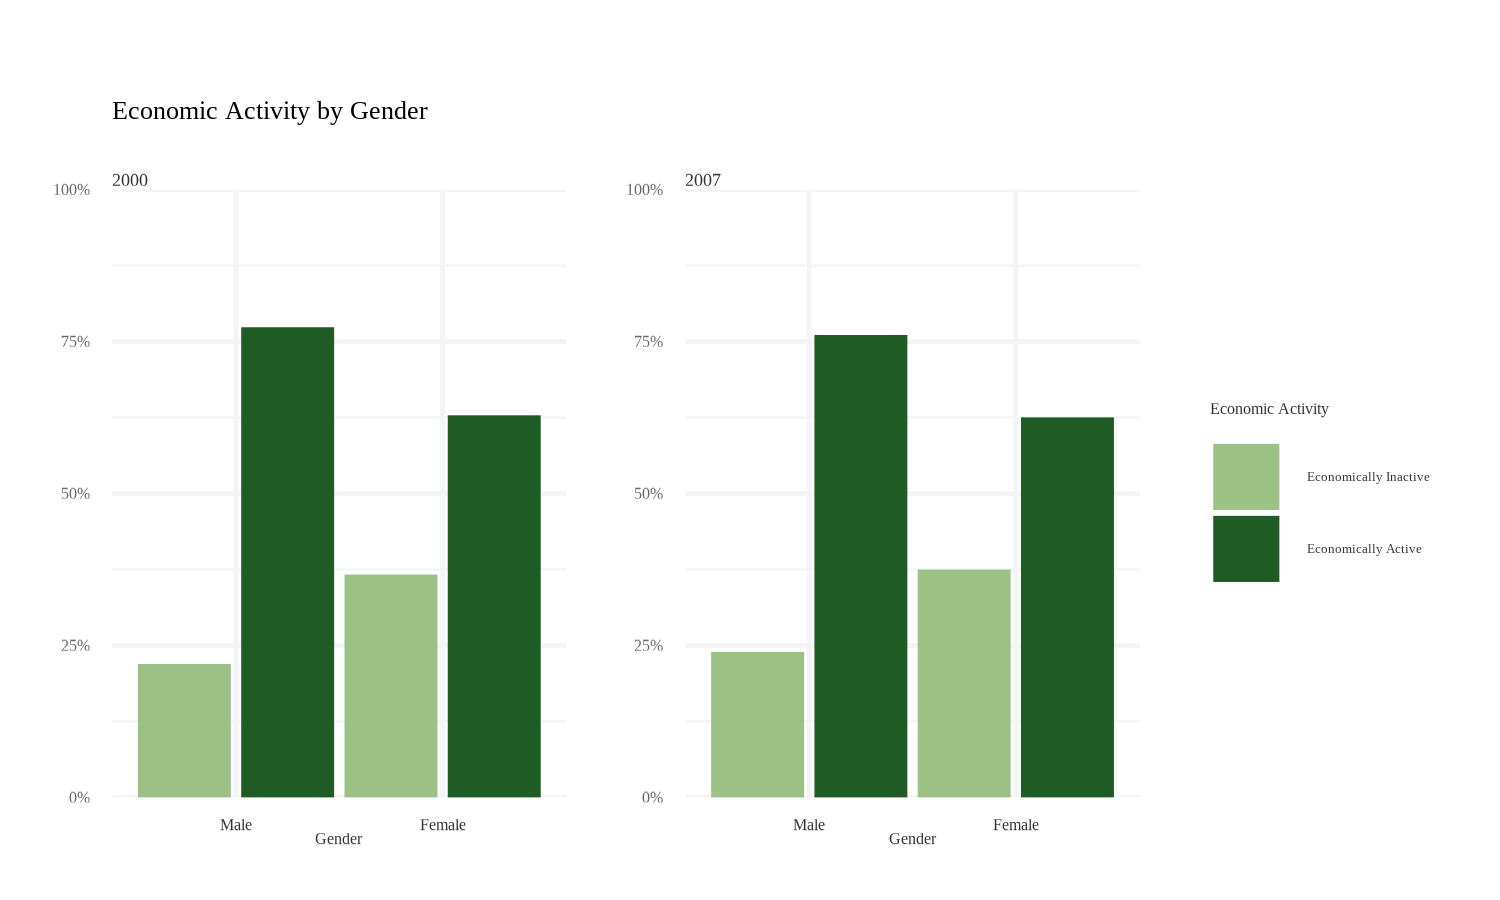
\includegraphics[width=500px,height=300px]{figure/econ_act_gen} \caption[Economic Activity and Gender]{Economic Activity and Gender in 2000 and 2007}\label{fig:econactgen}
\end{figure}
The data from the 2000 and 2007 survey waves reveal a persistent gender gap in economic activity, with males being more likely to be economically active than females. Specifically, in the 2000 survey wave, 78\% of males were economically active compared to 63\% of females, and in the 2007 survey wave, 76\% of males were economically active compared to 63\% of females. Additionally, in both survey waves, a higher percentage of females were economically inactive, with 37\% of females being economically inactive in both the 2000 and 2007 survey waves.

These findings are consistent with previous research on the gendered nature of employment and the structural barriers that women, particularly those from marginalized communities, face in accessing and maintaining economic opportunities (\protect\hyperlink{ref-RN4806}{McRobbie, 2020}).

It's important to note that the data should be interpreted with caution as it is a cross-sectional data and causality cannot be assumed, also the APMS data is based on self-reported measures and may be subject to bias. However, these findings highlight the need for more to be done that address structural inequalities, such as the gender pay gap, and support marginalized individuals, particularly women, in finding and maintaining economic activity. Furthermore, it's crucial to recognize the potential intersectionality of factors such as race, class, and disability that may compound these barriers.

\hypertarget{employment-status}{%
\subsection{Employment Status}\label{employment-status}}

For those individuals participating in the APMS who were economically active, several `types' of employment status were also recorded; employed, unemployed and unpaid worker.




\begin{figure}
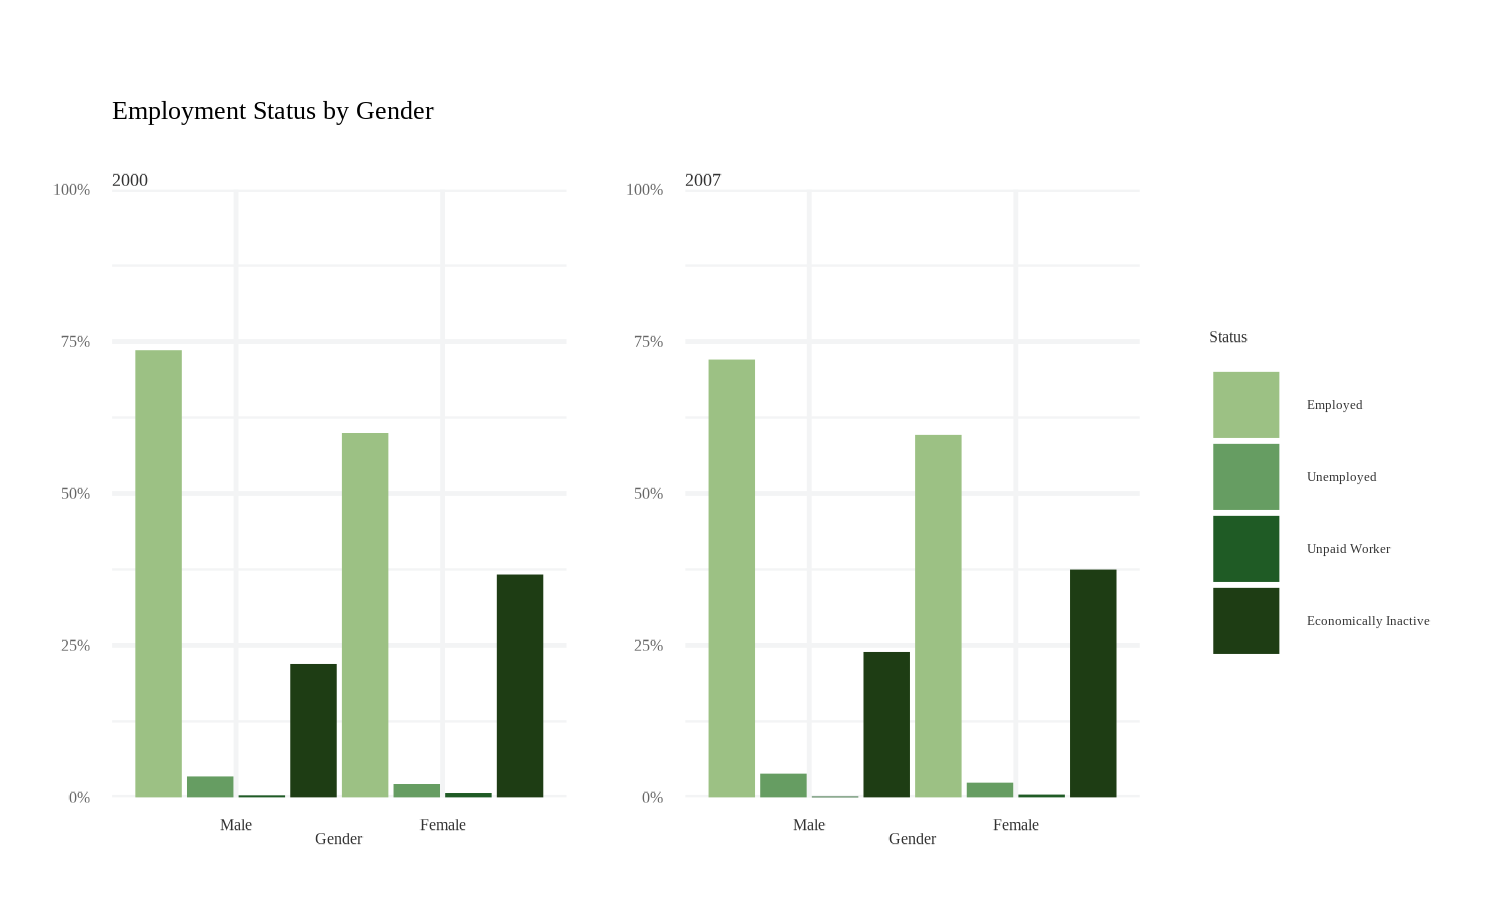
\includegraphics[width=500px,height=300px]{figure/at_gen} \caption[Employment Status and Gender]{Employment Status and Gender in 2000 and 2007}\label{fig:atgen}
\end{figure}
The analysis of employment status among individuals participating in the APMS survey between 2000 and 2007 reveals disparities in economic activity and employment opportunities based on gender. The data shows that a higher percentage of males were employed (74\% in 2000, 72\% in 2007) compared to females (60\% in 2000, 60\% in 2007). Furthermore, a higher percentage of males were unemployed (3.5\% in 2000, 3.9\% in 2007) compared to females (2.2\% in 2000, 2.4\% in 2007). Additionally, a higher percentage of unpaid workers were female (0.7\% in 2000, 0.5\% in 2007) compared to males (0.3\% in 2000, 0.1\% in 2007), highlighting the undervaluation and lack of recognition of care work and domestic labour, which disproportionately falls on women.

Furthermore, the data also reveals a disparity in unemployment rates between genders, with higher rates of male unemployment. This could be indicative of the gendered nature of the labour market, with specific sectors and industries being more male-dominated and less likely to provide job security and stability for men.
These findings reveal a significant gender gap in terms of employment opportunities and economic activity, which is reflective of the broader societal structures that perpetuate gender inequalities in the labour market. The data highlights the intersectionality of gender and class, as unpaid work is often associated with lower socioeconomic status and limited access to paid employment opportunities. This highlights the need for policies and programs that address these structural inequalities and support marginalized individuals, particularly women, in finding and maintaining economic activity.




\begin{figure}
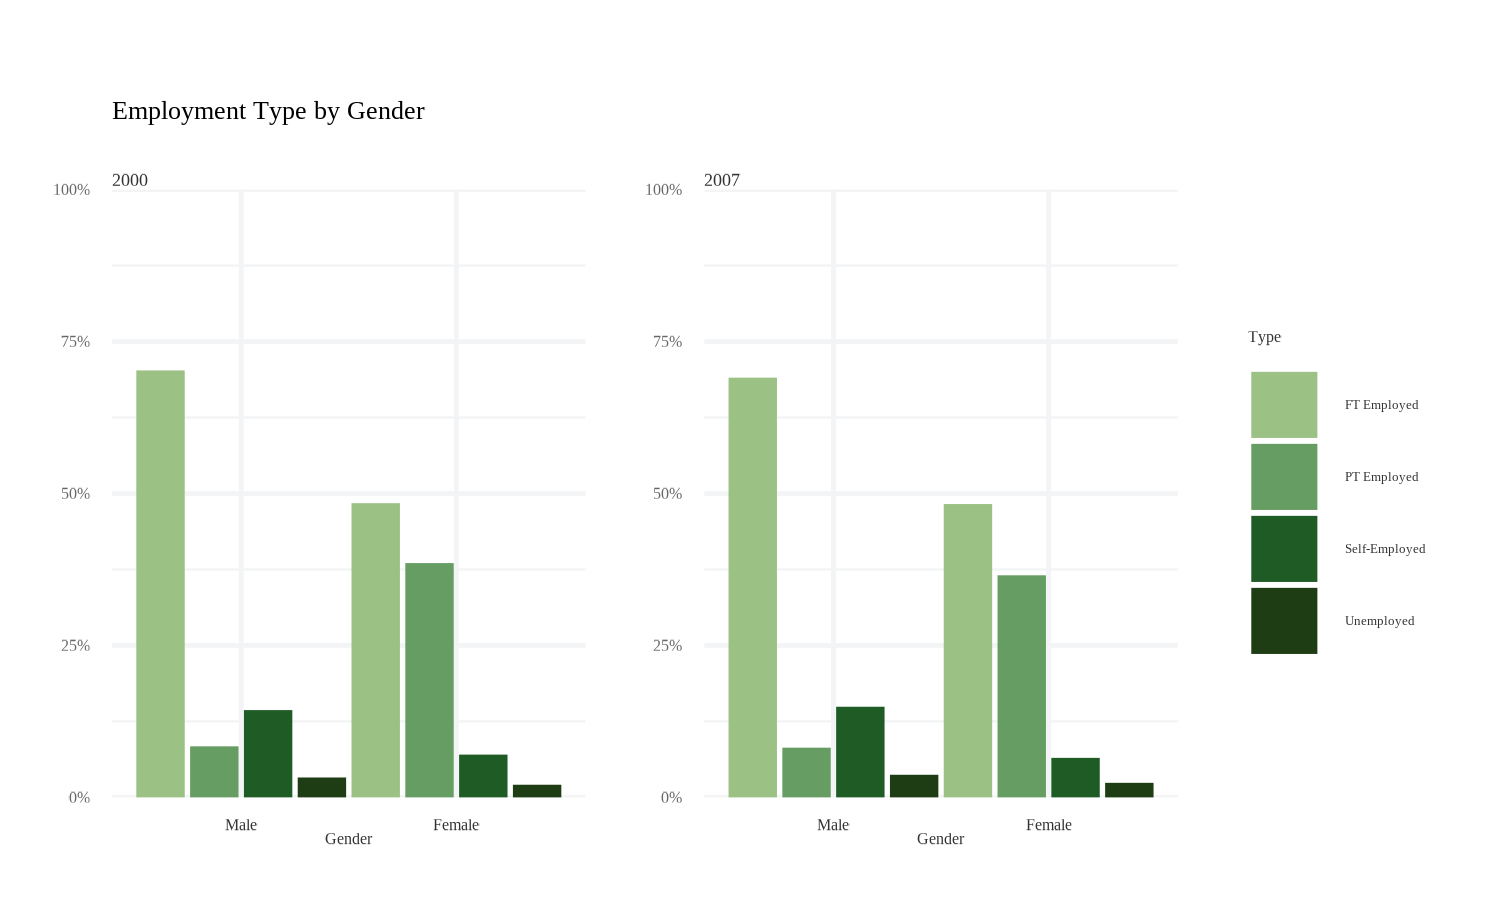
\includegraphics[width=500px,height=300px]{figure/et_gen} \caption[Employment Type and Gender]{Employment Type and Gender in 2000 and 2007}\label{fig:etgen}
\end{figure}
These findings reveal the intersectionality of gender, class, and labour market opportunities in England between 2000 and 2007. The data shows that in both survey waves, there were more males (73\% and 72\%) who were employed full-time than females (50\% and 52\%) and a higher proportion of females (40\% and 39\%) employed part-time than males (8.7\% and 8.5\%). Additionally, self-employment rates were also higher for men (15\% and 16\%) than for women (7.3\% and 6.9\%). This disparity in employment opportunities between genders is further highlighted by the unemployment rate, where a higher proportion of men (3.4\% and 3.9\%) were unemployed compared to women (2.2\% and 2.6\%). This data suggests that labour market opportunities for men and women in the UK at this time were not equal, with men having greater access to full-time employment and self-employment opportunities, while women were more likely to be employed part-time and unemployed. These findings underscore the need for policies and programs that address structural inequalities and support marginalized individuals, particularly women, in finding and maintaining employment. This may include targeted programs to increase access to full-time employment and self-employment opportunities for women, as well as policies that support work-life balance and address discrimination in the workplace. This could include initiatives such as targeted job training programs, flexible work arrangements, and parental leave policies that support women's economic participation and advancement. Additionally, addressing broader societal issues such as gender stereotypes and discrimination in the workplace is also important in promoting gender equality in the labour market.

\hypertarget{reasons-for-economic-inactivity}{%
\subsection{Reasons for Economic Inactivity}\label{reasons-for-economic-inactivity}}

For those part of the economically inactive group, they could indicate a reason for inactivity, including having a physical health condition, having a mental health condition, not being able to find a suitable job, or not wanting or not needing a job at the time of the survey.




\begin{figure}
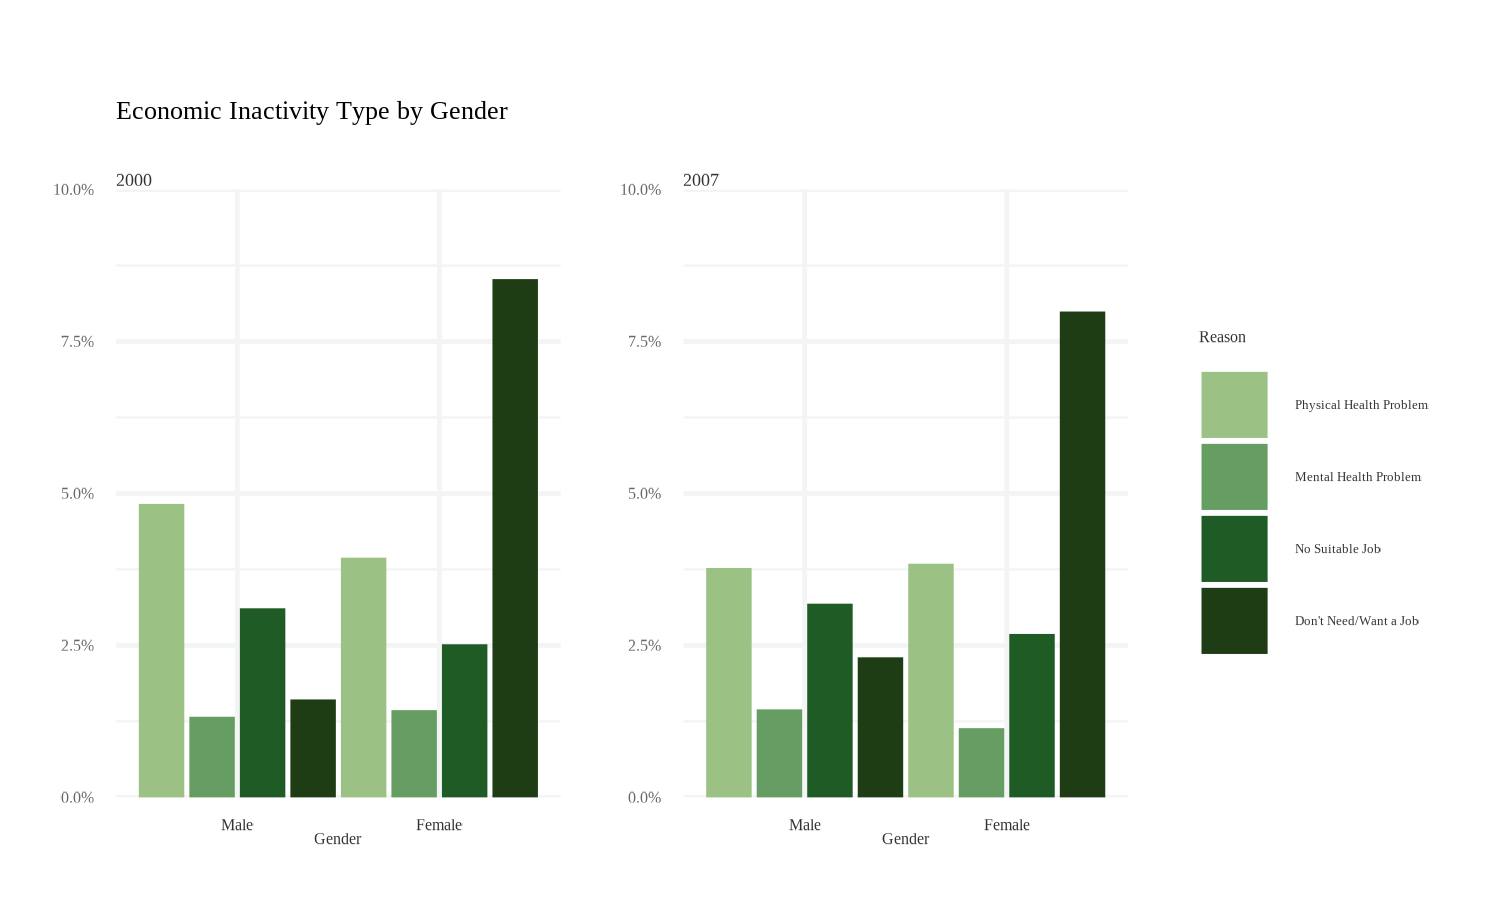
\includegraphics[width=500px,height=300px]{figure/inact} \caption[Reasons for Economic Inactivity and Gender]{Reasons for Economic Inactivity and Gender in 2000 and 2007}\label{fig:inact}
\end{figure}
The findings from the analysis reveal significant disparities in economic inactivity among different demographic groups in England. Specifically, the data shows that women were more likely to cite not wanting or needing a job at the time of the survey as a reason for economic inactivity, with 52\% of females indicating this in the 2000 survey wave and 51\% in the 2007 survey wave, compared to 15\% of males and 22\% of males respectively. This highlights the gendered nature of labour market opportunities and the societal expectation that women should prioritize care work and domestic responsibilities over paid employment.

Additionally, the data also shows that individuals living with physical health conditions were more likely to be economically inactive, with 32\% and 29\% of all individuals reporting this as a reason in the 2000 and 2007 survey waves respectively. This highlights the intersectionality of class and health in determining economic outcomes and the need for policies that support individuals with disabilities and chronic health conditions in finding and maintaining employment.

Furthermore, the data also shows that mental health issues were a relatively minor reason for economic inactivity, with only 10\% and 9.8\% of all individuals reporting this as a reason in the 2000 and 2007 survey waves respectively. However, this may be an underestimation as the social stigma surrounding mental health may have prevented some individuals from disclosing their struggles.

\hypertarget{economic-activity-and-age}{%
\subsection{Economic Activity and Age}\label{economic-activity-and-age}}

Age groups started at 16 years old and were capped at 74 years old to look at economic activity across the survey waves.




\begin{figure}
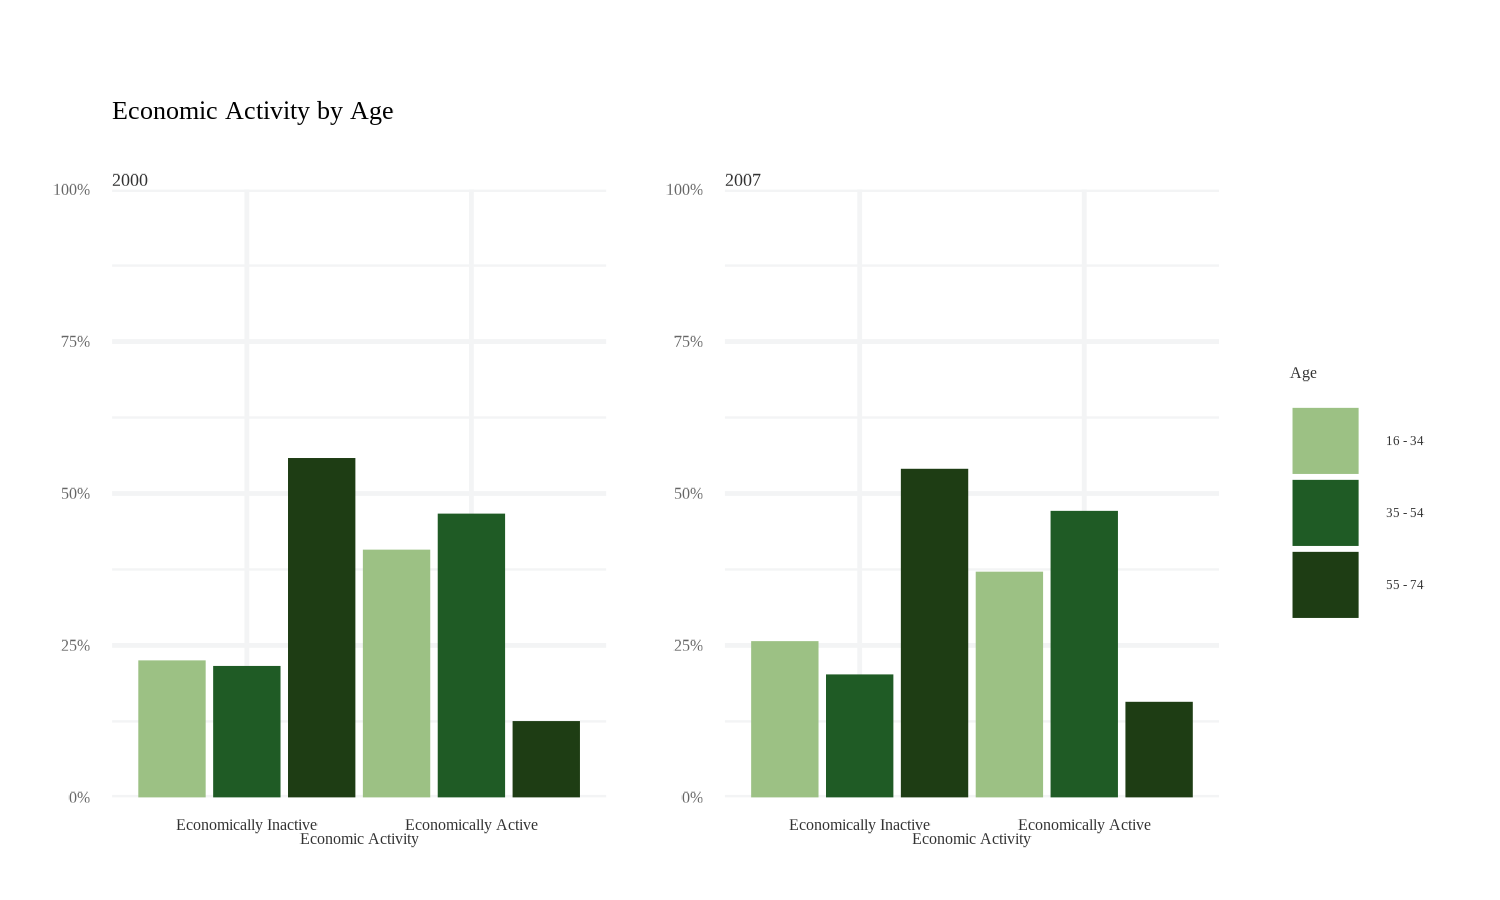
\includegraphics[width=500px,height=300px]{figure/emp_age} \caption[Economic Activity and Age]{Economic Activity and Age in 2000 and 2007}\label{fig:econactage}
\end{figure}
These findings reveal the intersectionality of age, class, and labour market opportunities, particularly for young adults and older individuals. For 16- to 34-year-olds, a significant majority were economically active in both 2000 and 2007, with 81\% and 76\% respectively. This highlights the challenges faced by young adults in finding and maintaining employment during this period. Similarly, for individuals aged 55-74, a majority were economically inactive in both 2000 and 2007, with 65\% and 60\% respectively.

One interesting observation is that there is a consistent pattern in the age groups' representation among individuals who are economically active and inactive across both survey waves. The largest age group, 35--54-year-olds, also has the highest percentage of economically active individuals. Additionally, older individuals (55--74-year-olds) have a higher percentage of economically inactive individuals. This highlights the barriers and discrimination that older individuals face in the labour market, particularly in terms of access to employment opportunities.

\hypertarget{economic-activity-and-education}{%
\subsection{Economic Activity and Education}\label{economic-activity-and-education}}

Educational qualifications consisted of; none (i.e., did not gain any qualifications), GCSE or their equivalent, A levels or their equivalent, a vocational degree, which were defined as nursing or teaching degrees, and a separate group for more traditional university degrees.




\begin{figure}
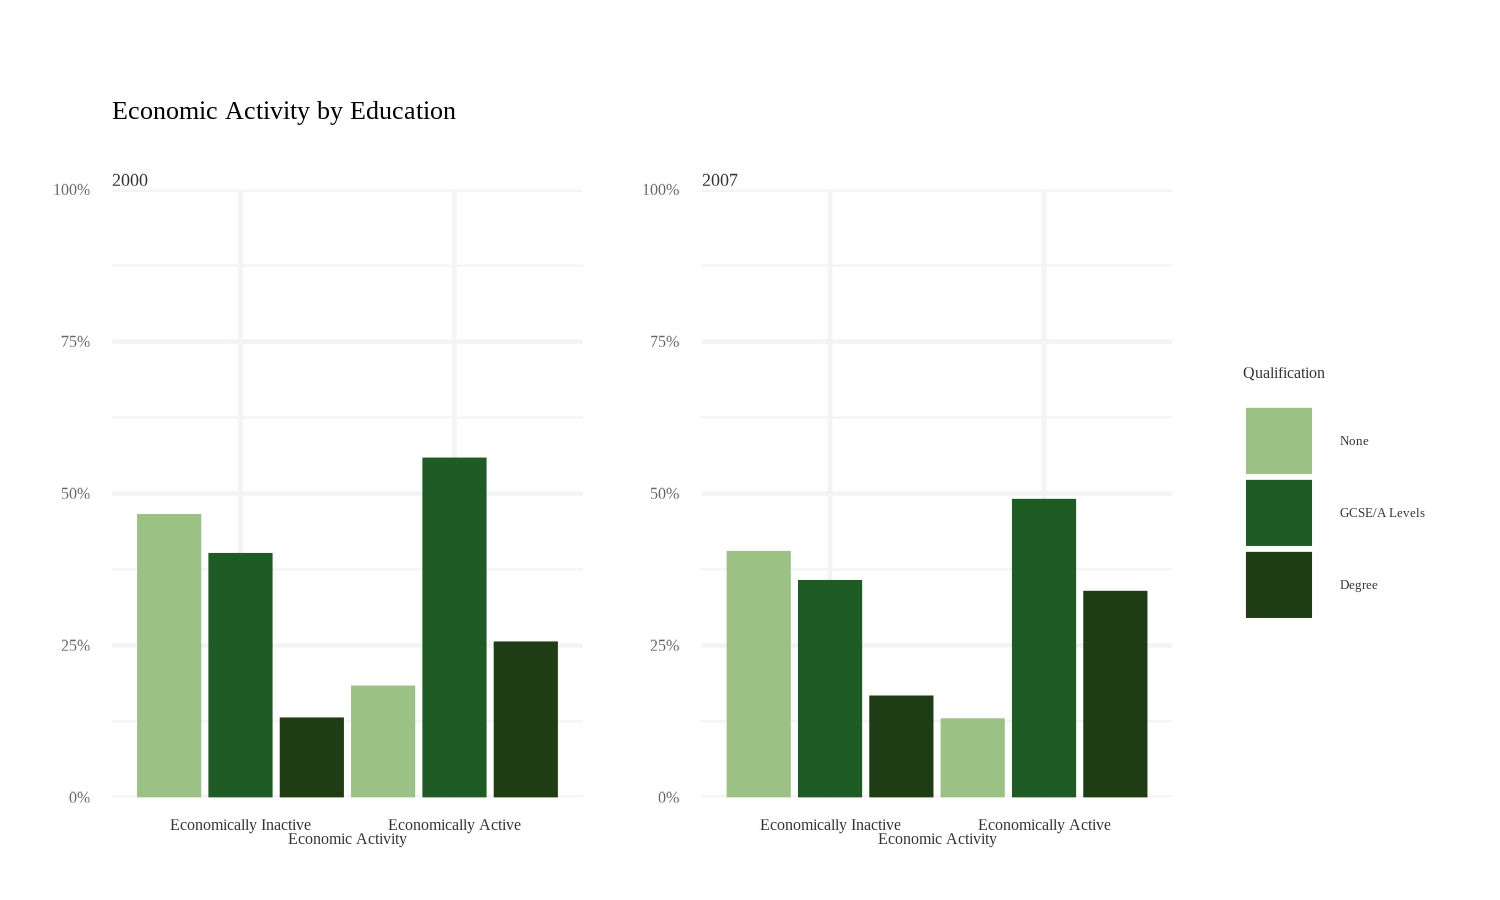
\includegraphics[width=500px,height=300px]{figure/emp_ed} \caption[Economic Activity and Education Group]{Economic Activity and Education in 2000 and 2007}\label{fig:econed}
\end{figure}
These data reveal the stark disparities in labour market opportunities and outcomes based on educational attainment, particularly for those with no qualifications. The high rates of economic inactivity among this group, with 47\% of those without educational qualifications being inactive in 2000 and 44\% in 2007, highlights the need for policies and programs that address the structural barriers preventing them from accessing and maintaining employment. Furthermore, these findings demonstrate the need for a more comprehensive approach to education that addresses the intersectionality of class, race, and gender, and supports marginalized individuals in gaining the necessary qualifications to enter and succeed in the labour market. The data also shows that having higher qualifications increases the chances of being economically active, with 56\% of those with GCSE and A level qualifications being active in 2000 and 51\% in 2007, and 26\% of those with a degree being active in 2000 and 35\% in 2007. However, the difference between someone with GCSE and A level qualifications and someone with a degree is not as significant as one might expect, which could indicate that the current educational system is not providing individuals with the skills and knowledge needed to secure stable employment in the 21st century.

There is a significant disparity in labour market opportunities and outcomes based on educational attainment. Individuals with no educational qualifications have a much higher rate of economic inactivity and a lower rate of economic activity compared to those with higher levels of education. This highlights the impact of systemic educational inequalities on economic outcomes and underscores the need for policies and programs that address these structural issues and support marginalized individuals, particularly those from lower socio-economic backgrounds, in achieving higher levels of education and gaining access to better job opportunities.

\hypertarget{economic-activity-and-social-class}{%
\subsection{Economic Activity and Social Class}\label{economic-activity-and-social-class}}

The AMPS survey waves measured indicators of social class via an adaptation of the Registrar General's Scale, with the options; Skilled or Unskilled. The primarily manual occupations were seen to map onto the working-class category, and the non-manual occupations were seen to map onto the middle-class category.




\begin{figure}
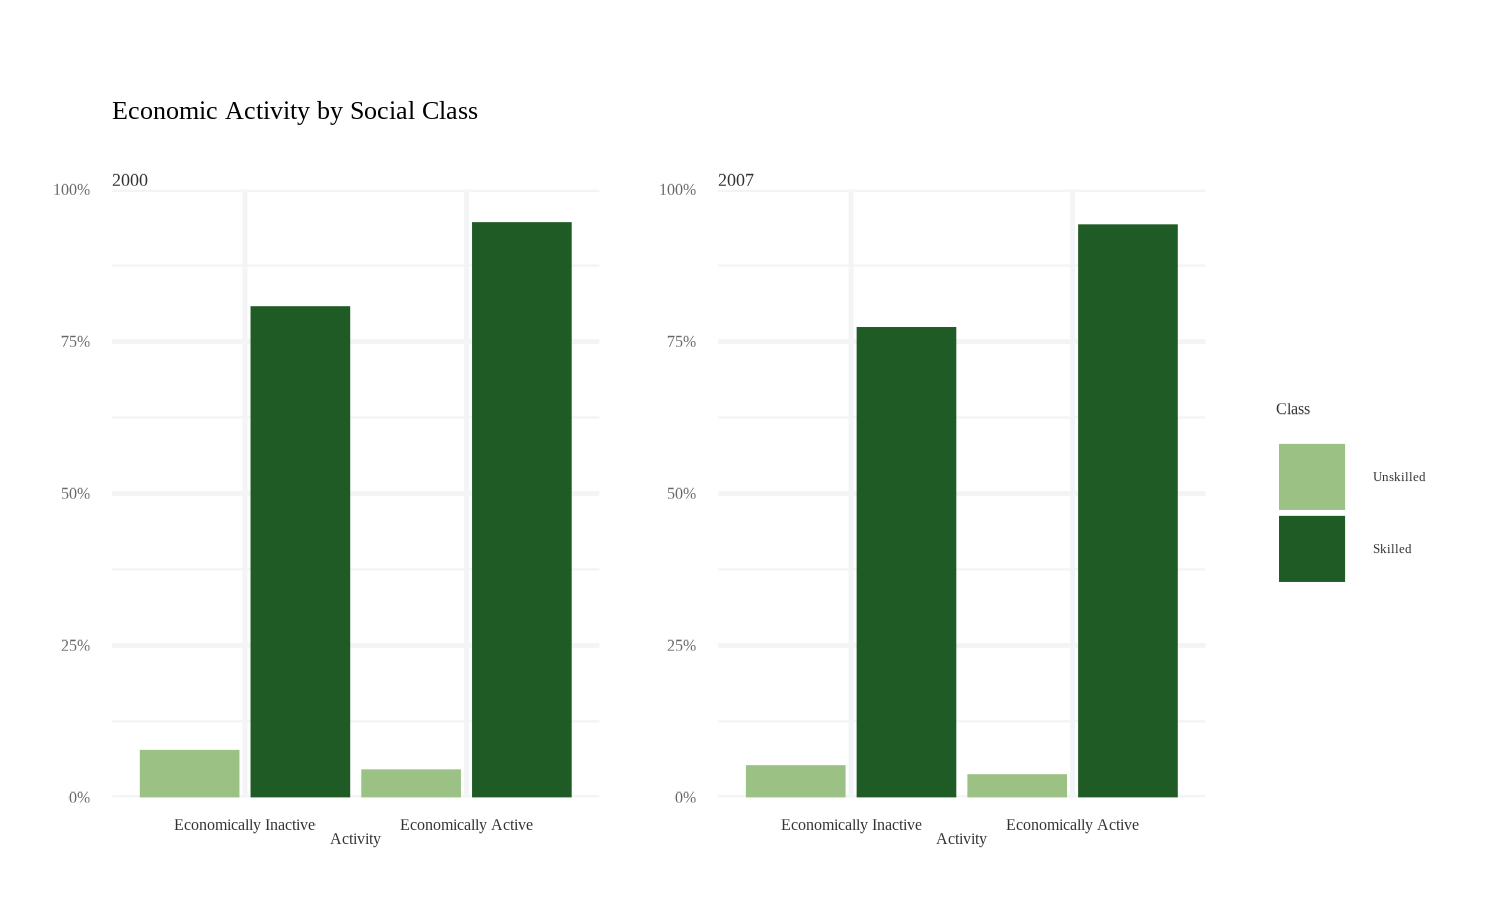
\includegraphics[width=500px,height=300px]{figure/econ_sc} \caption[Economic Activity and Social Class]{Economic Activity and Social Class in 2000 and 2007}\label{fig:econsc}
\end{figure}
The data from the 2000 and 2007 survey waves reveal the significant disparities in labour market opportunities and outcomes based on skill level, with those classified as ``unskilled'' disproportionately represented among the economically inactive population. Specifically, in the 2000 survey wave, 5.8\% of the overall sample were classified as unskilled, with 42\% of this group being economically inactive and 58\% being economically active. In contrast, 94\% of the overall sample were classified as skilled, with 26\% of this group being economically inactive and 74\% being economically active.

In the 2007 survey wave, the pattern remained similar, with 4.6\% of the overall sample classified as unskilled, and 38\% of this group being economically inactive and 62\% being economically active. Further, 95\% of the overall sample were classified as skilled, with 27\% of this group being economically inactive and 73\% being economically active. These findings highlight the need for policies and programs that address the structural barriers preventing unskilled individuals from accessing and maintaining employment, and the need for a more comprehensive approach to education and workforce development that addresses the intersectionality of class, race, and gender and supports marginalized individuals in gaining the necessary skills to enter and succeed in the labour market.

There is a clear correlation between skill level and economic activity. Individuals classified as ``unskilled'' make up a smaller percentage of the overall sample and are more likely to be economically inactive, while those classified as ``skilled'' make up a larger percentage of the sample and are more likely to be economically active. This highlights the importance of access to education and job training in order to improve economic opportunities and outcomes, particularly for those from marginalized backgrounds who may have less access to these resources. Additionally, this data also raises questions about the nature of ``unskilled'' work, and whether it is being fairly compensated and valued in society. This could be an indication that there is a need for policies that increase the minimum wage and labour rights for unskilled workers.

\hypertarget{economic-activity-and-ethnicity}{%
\subsection{Economic Activity and Ethnicity}\label{economic-activity-and-ethnicity}}

Ethnicity was measured via several options which were collapsed into: White or Other.




\begin{figure}
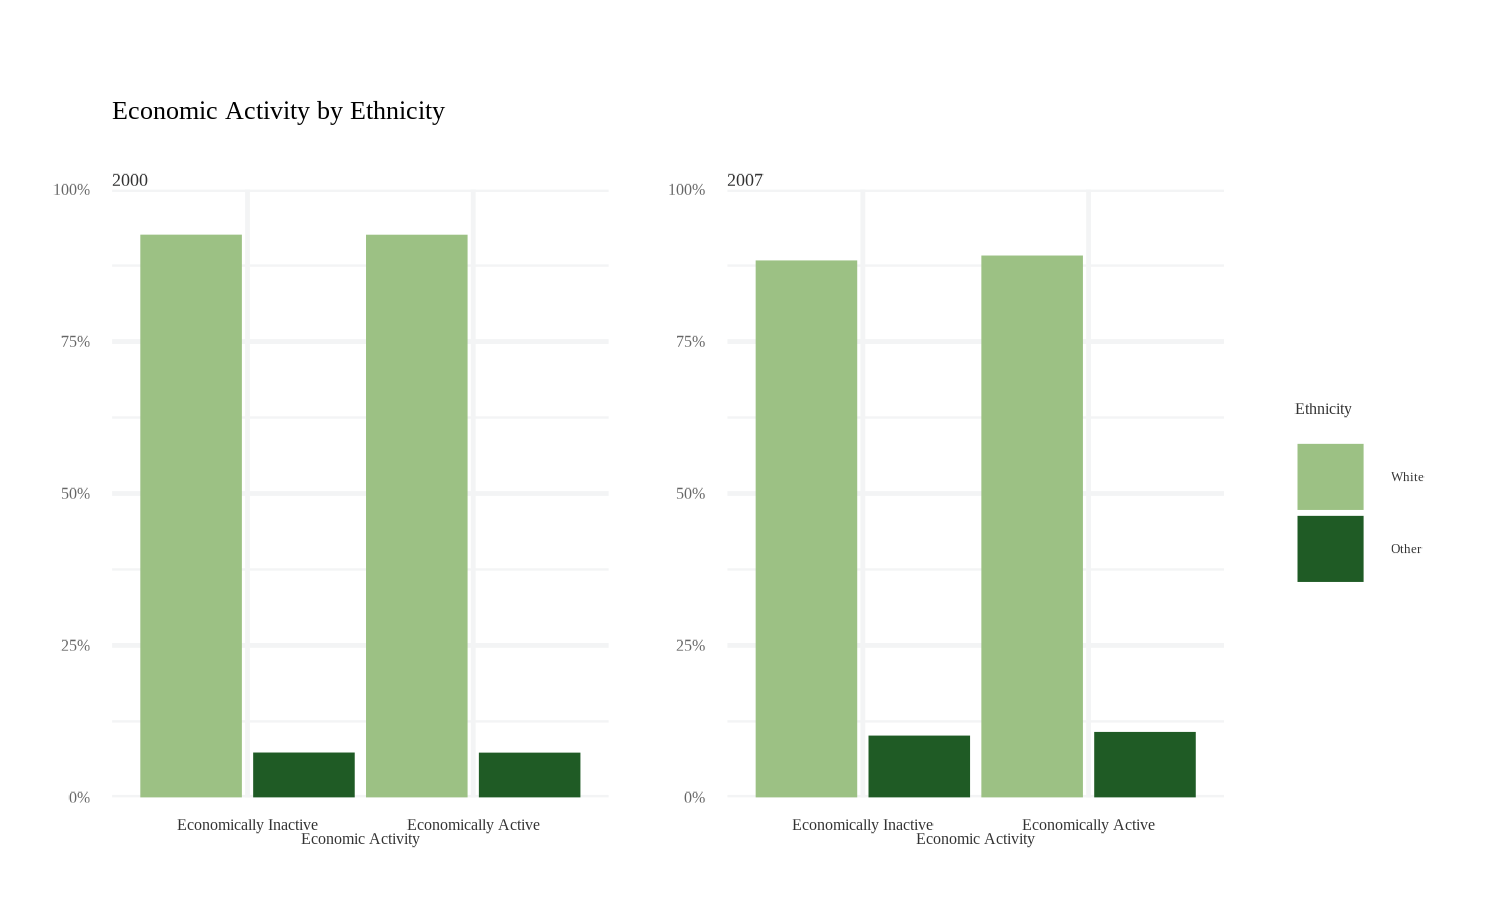
\includegraphics[width=500px,height=300px]{figure/econ_eth} \caption[Economic Activity and Ethnicity]{Economic Activity and Ethnicity in 2000 and 2007}\label{fig:econeth}
\end{figure}
The data from the 2000 survey wave indicates a stark disparity in labour market opportunities and outcomes based on ethnicity, particularly for individuals from ethnic minority backgrounds. The majority of the sample (93\%) identified as white, with an overall rate of 30\% being economically inactive and 70\% being active. Individuals from other ethnicities made up 7.4\% of the overall sample, with 30\% inactive and 70\% active. This highlights the need for policies and programs that address the structural barriers and discrimination that prevent individuals from ethnic minority backgrounds from accessing and maintaining employment.

In the 2007 survey wave, the pattern persisted with 89\% of the overall sample identifying as white, with 31\% being economically inactive and 69\% being active. Individuals from other ethnicities made up 11\% of the overall sample, with 30\% inactive and 70\% active. These findings reveal the persistent impact of systemic racial inequalities on economic outcomes and underscore the need for a more comprehensive approach to addressing structural racism in the labour market. This includes the development of targeted policies and programs that support marginalized individuals, particularly those from ethnic minority backgrounds, in gaining access to better job opportunities and achieving economic stability.

Interestingly while the percentage of white individuals in the sample decreased slightly between 2000 and 2007, the percentage of inactive individuals remained relatively consistent across both years and across different ethnicities, with around 30\% of individuals being inactive. This suggests that there may be structural factors that disproportionately impact individuals from different ethnicities and contribute to higher rates of economic inactivity, regardless of whether they are white or from other ethnicities. Additionally, the relatively consistent distribution of active and inactive individuals across different ethnicities suggests that there may be underlying issues of discrimination and bias within the labour market that affect individuals of different ethnicities similarly.

\hypertarget{economic-activity-and-physical-health}{%
\subsection{Economic Activity and Physical Health}\label{economic-activity-and-physical-health}}

Physical health was measured in a number of different ways, but presence of a physical health condition in this analysis was derived from individuals indicating they had sought medical help with a physical health issue in the months preceding being interviewed for the APMS.




\begin{figure}
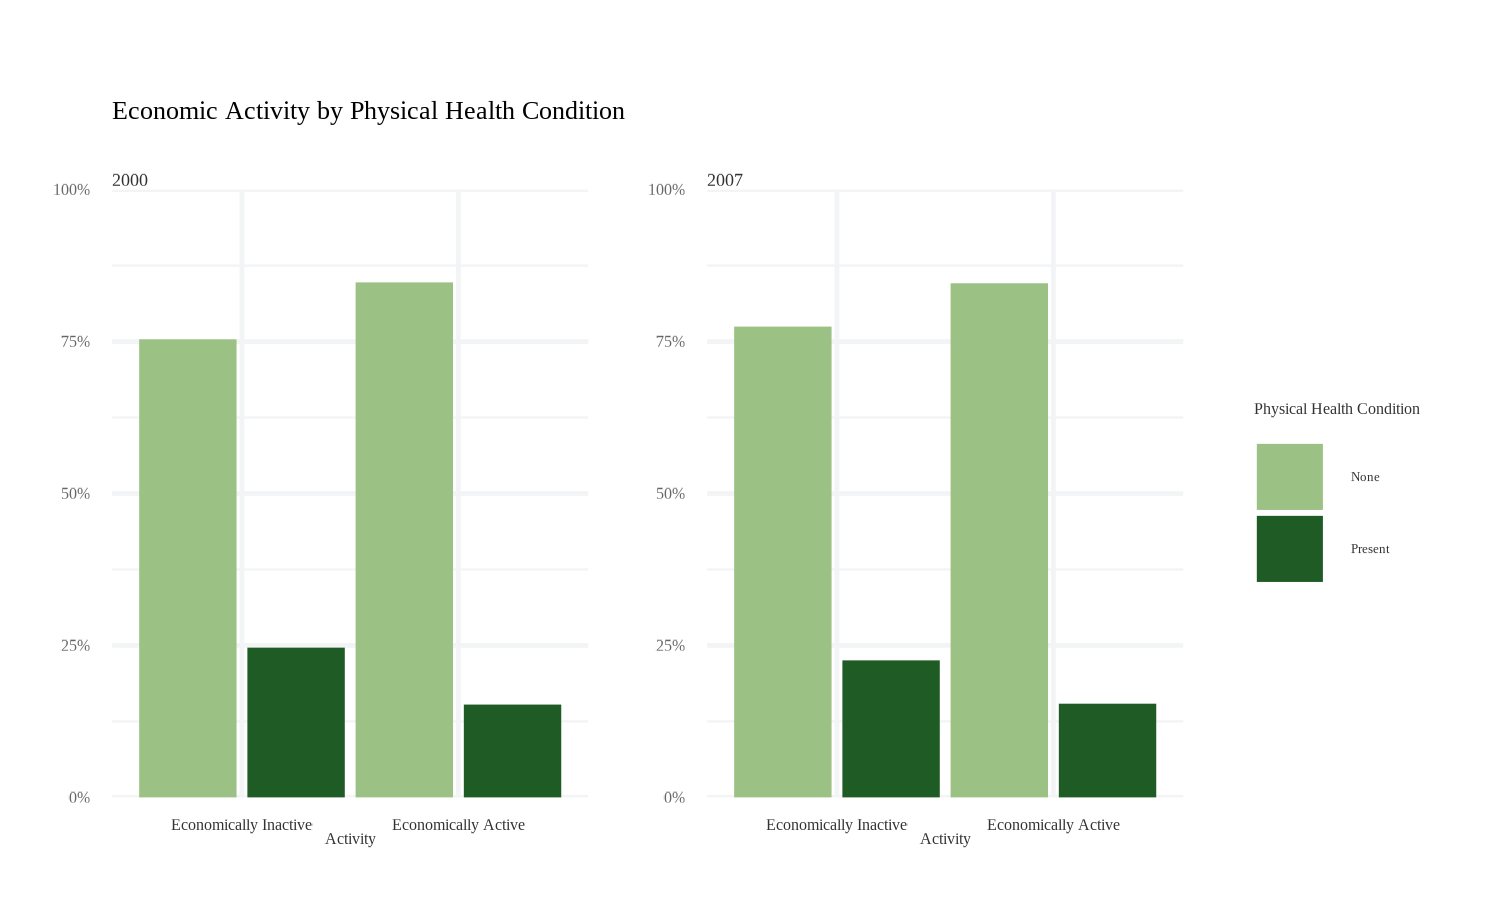
\includegraphics[width=500px,height=300px]{figure/econ_phc} \caption[Economic Activity and Physical Health Condition]{Economic Activity and Physical Health Condition in 2000 and 2007}\label{fig:econphc}
\end{figure}
The data from the 2000 and 2007 survey waves reveal a persistent pattern of individuals living with physical health conditions experiencing greater economic inactivity compared to those without physical health conditions. In the 2000 survey wave, 82\% of individuals reported not living with a physical health condition, with 85\% of these individuals being economically active and 75\% being economically inactive. In contrast, 18\% of individuals reported living with a physical health condition, with 15\% being economically active and 25\% being economically inactive.

Similarly, in the 2007 survey wave, 82\% of individuals reported not living with a physical health condition, with 85\% of these individuals being economically active and 77\% being economically inactive. In contrast, 18\% of individuals reported living with a physical health condition, with 15\% being economically active and 23\% being economically inactive. These findings underscore the need for policies and programs that address the structural barriers and discrimination faced by individuals living with physical health conditions and support them in accessing and maintaining employment.

The overall rate of individuals reporting not having a physical health condition was similar across both survey waves, at 82\%. However, a closer examination of the data shows that a higher proportion of these individuals were economically active in 2000 (85\%), as compared to 2007 (85\%). Additionally, a higher proportion of individuals living with a physical health condition were economically inactive in 2000 (25\%), as compared to 2007 (23\%). These findings highlight the impact of physical health conditions on economic outcomes and underscore the need for policies and programs that support individuals living with physical health conditions in accessing and maintaining employment.

\hypertarget{economic-activity-and-treatment-use}{%
\subsection{Economic Activity and Treatment Use}\label{economic-activity-and-treatment-use}}

Treatment use encompassed any treatment for a mental health condition and included any medication, counselling, or therapy, both, and no treatment at all.




\begin{figure}
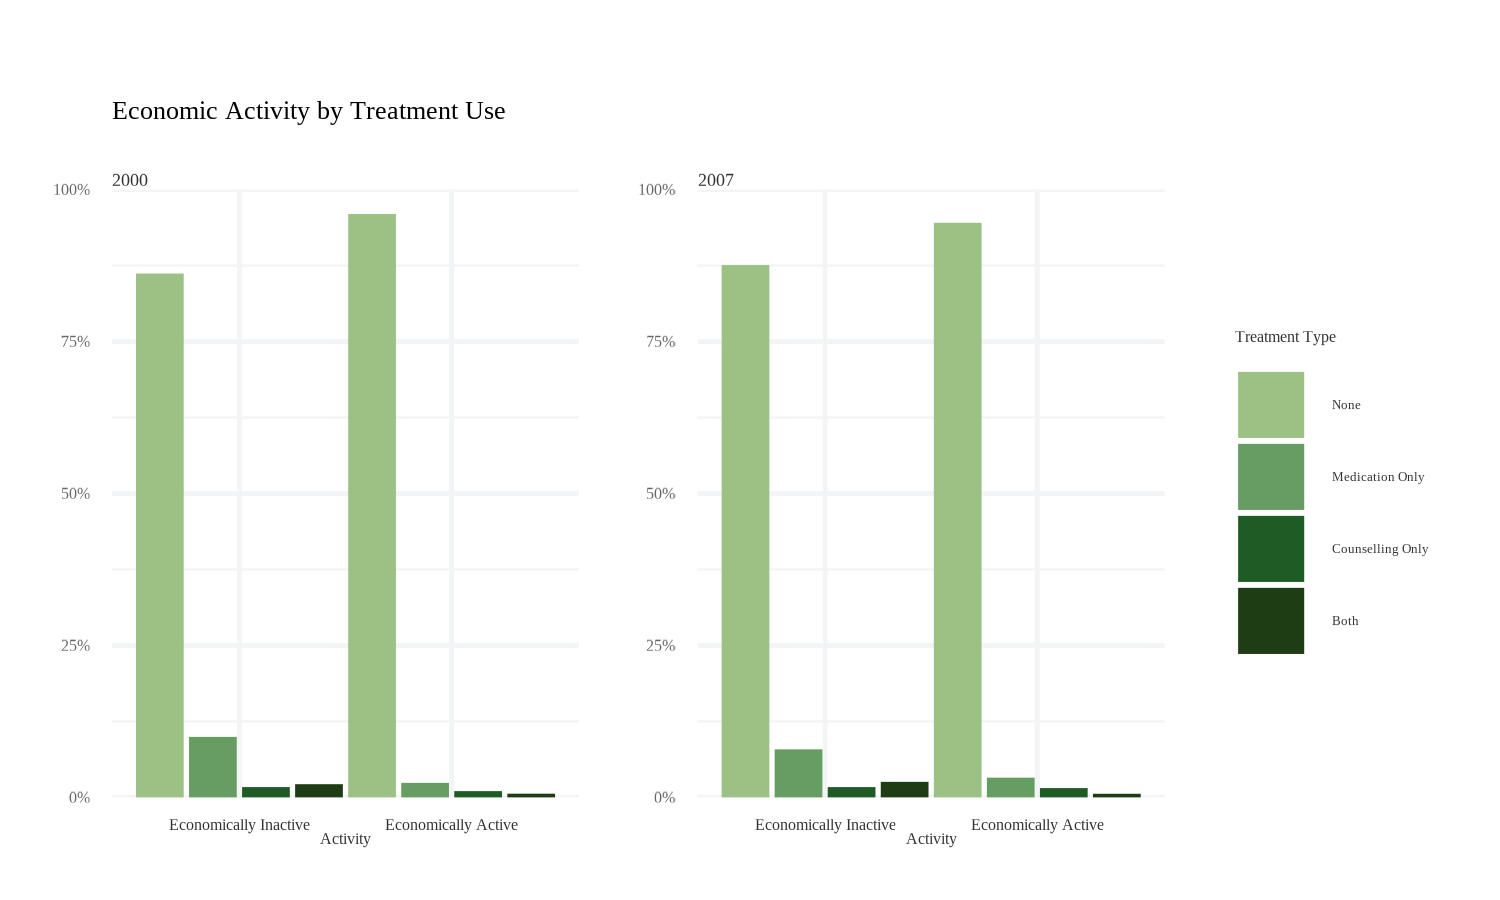
\includegraphics[width=500px,height=300px]{figure/econ_trt} \caption[Economic Activity and Treatment Use]{Economic Activity and Treatment Use in 2000 and 2007}\label{fig:econtrt}
\end{figure}
The data from the 2000 and 2007 survey waves in the UK reveals the relationship between treatment for mental health conditions and economic activity. A majority of individuals in both waves reported not receiving any treatment at all, with an overall rate of 93\%. The most common form of treatment reported was medication only, with an overall rate of 4.6\% and 4.7\% respectively. These findings highlight the need for policies and programs that address the barriers to accessing mental health treatment and support individuals with mental health conditions in finding and maintaining employment. Furthermore, it is important to note that the data also shows that while receiving any form of treatment may increase the chance of being economically active, the rates of active individuals among those who reported receiving medication only, counselling or therapy only or both, were low. This could indicate that the current mental health treatment system is not providing individuals with the necessary support to secure stable employment, and that a more comprehensive approach is needed to address this issue.

This observation highlights the intersectionality of mental health and economic outcomes. The data suggests that despite receiving treatment, individuals with mental health conditions still face significant barriers to accessing and maintaining employment. This could be due to a lack of support or accommodations in the workplace, discrimination and stigma, or a lack of understanding among employers about how to support employees with mental health conditions. Additionally, the low rates of active individuals among those who reported receiving medication only, counseling or therapy only, or both, suggests that current mental health treatment may not be adequate to address the unique needs of individuals with mental health conditions, particularly as it relates to their ability to participate in the workforce.

This observation underscores the need for policies and programs that address structural barriers and support marginalized individuals, particularly those with mental health conditions, in finding and maintaining employment. Additionally, it highlights the need for a more comprehensive approach to mental health treatment, that addresses the intersectionality of mental health, class, race, and gender, and supports marginalized individuals in gaining the necessary support to enter and succeed in the labour market.

\hypertarget{economic-activity-and-mental-health-service-use}{%
\subsection{Economic Activity and Mental Health Service Use}\label{economic-activity-and-mental-health-service-use}}

Engaging with mental health services was derived from individuals reporting that they had received health care for a mental health condition, including their GP, inpatient and outpatient hospital appointments and community mental health teams.




\begin{figure}
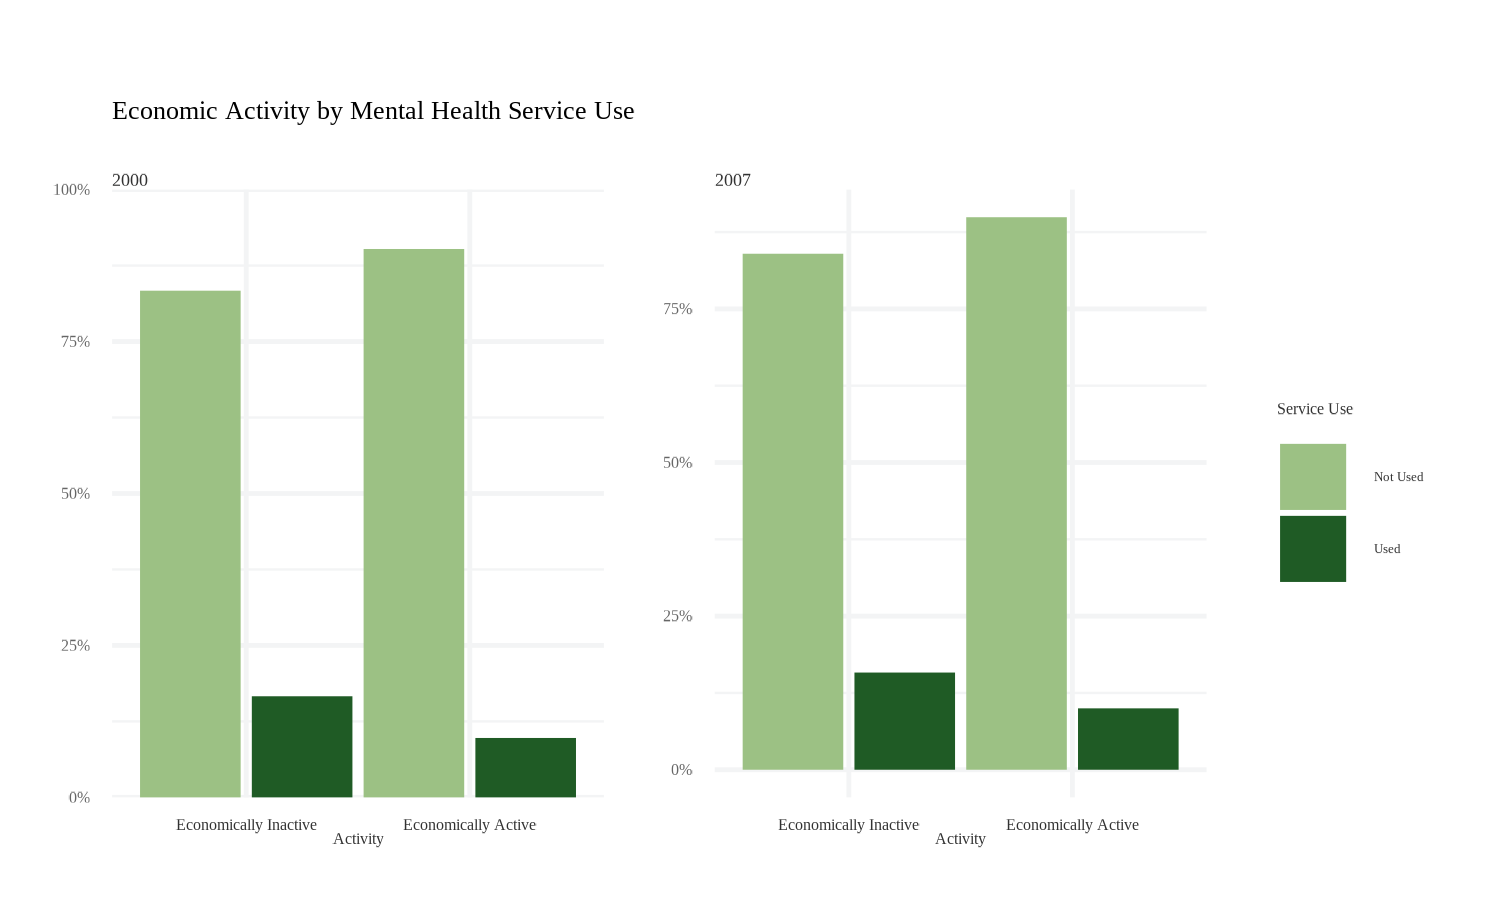
\includegraphics[width=500px,height=300px]{figure/econ_su} \caption[Economic Activity and Mental Health Service Use]{Economic Activity and Mental Health Service Use in 2000 and 2007}\label{fig:econsu}
\end{figure}
The data from the 2000 and 2007 survey waves reveal a significant disparity in labour market opportunities and outcomes for individuals who have accessed mental health services compared to those who have not. Specifically, the 2000 survey wave showed that 88\% of individuals reported as having not used any mental health service, with 90\% of those reporting as being economically active and 83\% reporting being economically inactive. Of those individuals that did report as using a mental health service, the overall rate was 12\%, with 9.8\% of those reporting as being economically active and 17\% reporting as being economically inactive. Similarly, in the 2007 survey wave, the majority of individuals reported as not having used any mental health service, with an overall rate of 88\%, with 90\% of these individuals being economically active and 84\% being economically inactive. For the individuals that did indicate that they had used mental health services, the overall rate was 12\%, with 10.0\% of these individuals reporting being economically active, and 16\% reporting as being economically inactive. The high rates of economic inactivity among those who have used mental health services highlights the need for policies and programs that address the structural barriers preventing them from accessing and maintaining employment. Furthermore, these findings demonstrate the need for a more comprehensive approach to mental health that addresses the intersectionality of class, race, and gender, and supports marginalized individuals in receiving the necessary support to secure and maintain employment.

In the context of labour market opportunities and outcomes, intersectionality can help to explain why certain individuals, such as women of color or low-income queer individuals, may face additional barriers to accessing and maintaining employment compared to those who only face discrimination based on one aspect of their identity. It highlights the need for policies and programs that consider the unique experiences and needs of marginalized communities and addresses the multiple forms of oppression they may face.

For example, programs that focus solely on increasing the number of women in the workforce may not address the specific barriers faced by women of color or low-income women. Similarly, mental health services that primarily serve cisgender, middle-class, able-bodied individuals may not be accessible or appropriate for individuals from marginalized communities. Therefore, an intersectional approach would ensure that these policies and programs address the specific needs of marginalized communities and provide more equitable access to employment opportunities and support services.

\hypertarget{common-mental-health-disorders}{%
\section{Common Mental Health Disorders}\label{common-mental-health-disorders}}

\hypertarget{sample-overview}{%
\subsection{Sample Overview}\label{sample-overview}}

Breaking the survey waves down by common mental health disorders presence shows statistically significant relationships in the majority of variables in Table \ref{tab:results1-charcmd}.

\providecommand{\huxb}[2]{\arrayrulecolor[RGB]{#1}\global\arrayrulewidth=#2pt}
  \providecommand{\huxvb}[2]{\color[RGB]{#1}\vrule width #2pt}
  \providecommand{\huxtpad}[1]{\rule{0pt}{#1}}
  \providecommand{\huxbpad}[1]{\rule[-#1]{0pt}{#1}}
\begin{table}[ht]
\begin{centerbox}
\begin{threeparttable}
 \setlength{\tabcolsep}{0pt}
\begin{adjustbox}{width=1\textwidth}
\large
\begin{tabular}{l l l l l l l l l l l}


\hhline{>{\arrayrulecolor[RGB]{0, 0, 0}\global\arrayrulewidth=0.4pt}->{\arrayrulecolor[RGB]{0, 0, 0}\global\arrayrulewidth=0.4pt}->{\arrayrulecolor[RGB]{0, 0, 0}\global\arrayrulewidth=0.4pt}->{\arrayrulecolor[RGB]{0, 0, 0}\global\arrayrulewidth=0.4pt}->{\arrayrulecolor[RGB]{0, 0, 0}\global\arrayrulewidth=0.4pt}->{\arrayrulecolor[RGB]{0, 0, 0}\global\arrayrulewidth=0.4pt}->{\arrayrulecolor[RGB]{0, 0, 0}\global\arrayrulewidth=0.4pt}->{\arrayrulecolor[RGB]{0, 0, 0}\global\arrayrulewidth=0.4pt}->{\arrayrulecolor[RGB]{0, 0, 0}\global\arrayrulewidth=0.4pt}->{\arrayrulecolor[RGB]{0, 0, 0}\global\arrayrulewidth=0.4pt}->{\arrayrulecolor[RGB]{0, 0, 0}\global\arrayrulewidth=0.4pt}-}
\arrayrulecolor{black}

\multicolumn{1}{!{\color[RGB]{0, 0, 0}\vrule width 0pt}l!{\color[RGB]{0, 0, 0}\vrule width 0pt}}{\rule{0pt}{1pt + 1em}\raggedright \hspace{0pt} \textbf{{\fontsize{14pt}{16.8pt}\selectfont 
}} \hspace{1pt}\rule[-1pt]{0pt}{1pt}} &
\multicolumn{5}{c!{\color[RGB]{0, 0, 0}\vrule width 0pt}}{\rule{0pt}{1pt + 1em}\centering \hspace{1pt} \textbf{{\fontsize{14pt}{16.8pt}\selectfont \textbf{2000 Wave}
}} \hspace{1pt}\rule[-1pt]{0pt}{1pt}} &
\multicolumn{5}{c!{\color[RGB]{0, 0, 0}\vrule width 0pt}}{\rule{0pt}{1pt + 1em}\centering \hspace{1pt} \textbf{{\fontsize{14pt}{16.8pt}\selectfont \textbf{2007 Wave}
}} \hspace{1pt}\rule[-1pt]{0pt}{1pt}} \tabularnewline[-0.5pt]


\hhline{}
\arrayrulecolor{black}

\multicolumn{1}{!{\color[RGB]{0, 0, 0}\vrule width 0pt}l!{\color[RGB]{0, 0, 0}\vrule width 0pt}}{\rule{0pt}{1pt + 1em}\raggedright \hspace{0pt} \textbf{{\fontsize{14pt}{16.8pt}\selectfont \textbf{Characteristic}
}} \hspace{1pt}\rule[-1pt]{0pt}{1pt}} &
\multicolumn{1}{c!{\color[RGB]{0, 0, 0}\vrule width 0pt}}{\rule{0pt}{1pt + 1em}\centering \hspace{1pt} \textbf{{\fontsize{14pt}{16.8pt}\selectfont \textbf{N}
}} \hspace{1pt}\rule[-1pt]{0pt}{1pt}} &
\multicolumn{1}{c!{\color[RGB]{0, 0, 0}\vrule width 0pt}}{\rule{0pt}{1pt + 1em}\centering \hspace{1pt} \textbf{{\fontsize{14pt}{16.8pt}\selectfont \textbf{Overall}, N = 7,247
}} \hspace{1pt}\rule[-1pt]{0pt}{1pt}} &
\multicolumn{1}{c!{\color[RGB]{0, 0, 0}\vrule width 0pt}}{\rule{0pt}{1pt + 1em}\centering \hspace{1pt} \textbf{{\fontsize{14pt}{16.8pt}\selectfont \textbf{None}, N = 6,048
}} \hspace{1pt}\rule[-1pt]{0pt}{1pt}} &
\multicolumn{1}{c!{\color[RGB]{0, 0, 0}\vrule width 0pt}}{\rule{0pt}{1pt + 1em}\centering \hspace{1pt} \textbf{{\fontsize{14pt}{16.8pt}\selectfont \textbf{Present}, N = 1,199
}} \hspace{1pt}\rule[-1pt]{0pt}{1pt}} &
\multicolumn{1}{c!{\color[RGB]{0, 0, 0}\vrule width 0pt}}{\rule{0pt}{1pt + 1em}\centering \hspace{1pt} \textbf{{\fontsize{14pt}{16.8pt}\selectfont \textbf{p-value}
}} \hspace{1pt}\rule[-1pt]{0pt}{1pt}} &
\multicolumn{1}{c!{\color[RGB]{0, 0, 0}\vrule width 0pt}}{\rule{0pt}{1pt + 1em}\centering \hspace{1pt} \textbf{{\fontsize{14pt}{16.8pt}\selectfont \textbf{N}
}} \hspace{1pt}\rule[-1pt]{0pt}{1pt}} &
\multicolumn{1}{c!{\color[RGB]{0, 0, 0}\vrule width 0pt}}{\rule{0pt}{1pt + 1em}\centering \hspace{1pt} \textbf{{\fontsize{14pt}{16.8pt}\selectfont \textbf{Overall}, N = 6,453
}} \hspace{1pt}\rule[-1pt]{0pt}{1pt}} &
\multicolumn{1}{c!{\color[RGB]{0, 0, 0}\vrule width 0pt}}{\rule{0pt}{1pt + 1em}\centering \hspace{1pt} \textbf{{\fontsize{14pt}{16.8pt}\selectfont \textbf{None}, N = 5,365
}} \hspace{1pt}\rule[-1pt]{0pt}{1pt}} &
\multicolumn{1}{c!{\color[RGB]{0, 0, 0}\vrule width 0pt}}{\rule{0pt}{1pt + 1em}\centering \hspace{1pt} \textbf{{\fontsize{14pt}{16.8pt}\selectfont \textbf{Present}, N = 1,088
}} \hspace{1pt}\rule[-1pt]{0pt}{1pt}} &
\multicolumn{1}{c!{\color[RGB]{0, 0, 0}\vrule width 0pt}}{\rule{0pt}{1pt + 1em}\centering \hspace{1pt} \textbf{{\fontsize{14pt}{16.8pt}\selectfont \textbf{p-value}
}} \hspace{0pt}\rule[-1pt]{0pt}{1pt}} \tabularnewline[-0.5pt]


\hhline{>{\arrayrulecolor[RGB]{0, 0, 0}\global\arrayrulewidth=0.4pt}->{\arrayrulecolor[RGB]{0, 0, 0}\global\arrayrulewidth=0.4pt}->{\arrayrulecolor[RGB]{0, 0, 0}\global\arrayrulewidth=0.4pt}->{\arrayrulecolor[RGB]{0, 0, 0}\global\arrayrulewidth=0.4pt}->{\arrayrulecolor[RGB]{0, 0, 0}\global\arrayrulewidth=0.4pt}->{\arrayrulecolor[RGB]{0, 0, 0}\global\arrayrulewidth=0.4pt}->{\arrayrulecolor[RGB]{0, 0, 0}\global\arrayrulewidth=0.4pt}->{\arrayrulecolor[RGB]{0, 0, 0}\global\arrayrulewidth=0.4pt}->{\arrayrulecolor[RGB]{0, 0, 0}\global\arrayrulewidth=0.4pt}->{\arrayrulecolor[RGB]{0, 0, 0}\global\arrayrulewidth=0.4pt}->{\arrayrulecolor[RGB]{0, 0, 0}\global\arrayrulewidth=0.4pt}-}
\arrayrulecolor{black}

\multicolumn{1}{!{\color[RGB]{0, 0, 0}\vrule width 0pt}l!{\color[RGB]{0, 0, 0}\vrule width 0pt}}{\rule{0pt}{1pt + 1em}\raggedright \hspace{0pt} \textbf{{\fontsize{14pt}{16.8pt}\selectfont Age}} \hspace{1pt}\rule[-1pt]{0pt}{1pt}} &
\multicolumn{1}{c!{\color[RGB]{0, 0, 0}\vrule width 0pt}}{\rule{0pt}{1pt + 1em}\centering \hspace{1pt} {\fontsize{14pt}{16.8pt}\selectfont 7,247} \hspace{1pt}\rule[-1pt]{0pt}{1pt}} &
\multicolumn{1}{c!{\color[RGB]{0, 0, 0}\vrule width 0pt}}{\rule{0pt}{1pt + 1em}\centering \hspace{1pt} {\fontsize{14pt}{16.8pt}\selectfont 43 (16)} \hspace{1pt}\rule[-1pt]{0pt}{1pt}} &
\multicolumn{1}{c!{\color[RGB]{0, 0, 0}\vrule width 0pt}}{\rule{0pt}{1pt + 1em}\centering \hspace{1pt} {\fontsize{14pt}{16.8pt}\selectfont 43 (16)} \hspace{1pt}\rule[-1pt]{0pt}{1pt}} &
\multicolumn{1}{c!{\color[RGB]{0, 0, 0}\vrule width 0pt}}{\rule{0pt}{1pt + 1em}\centering \hspace{1pt} {\fontsize{14pt}{16.8pt}\selectfont 41 (14)} \hspace{1pt}\rule[-1pt]{0pt}{1pt}} &
\multicolumn{1}{c!{\color[RGB]{0, 0, 0}\vrule width 0pt}}{\rule{0pt}{1pt + 1em}\centering \hspace{1pt} \textbf{{\fontsize{14pt}{16.8pt}\selectfont 0.014}} \hspace{1pt}\rule[-1pt]{0pt}{1pt}} &
\multicolumn{1}{c!{\color[RGB]{0, 0, 0}\vrule width 0pt}}{\rule{0pt}{1pt + 1em}\centering \hspace{1pt} {\fontsize{14pt}{16.8pt}\selectfont 6,453} \hspace{1pt}\rule[-1pt]{0pt}{1pt}} &
\multicolumn{1}{c!{\color[RGB]{0, 0, 0}\vrule width 0pt}}{\rule{0pt}{1pt + 1em}\centering \hspace{1pt} {\fontsize{14pt}{16.8pt}\selectfont 43 (16)} \hspace{1pt}\rule[-1pt]{0pt}{1pt}} &
\multicolumn{1}{c!{\color[RGB]{0, 0, 0}\vrule width 0pt}}{\rule{0pt}{1pt + 1em}\centering \hspace{1pt} {\fontsize{14pt}{16.8pt}\selectfont 43 (16)} \hspace{1pt}\rule[-1pt]{0pt}{1pt}} &
\multicolumn{1}{c!{\color[RGB]{0, 0, 0}\vrule width 0pt}}{\rule{0pt}{1pt + 1em}\centering \hspace{1pt} {\fontsize{14pt}{16.8pt}\selectfont 41 (15)} \hspace{1pt}\rule[-1pt]{0pt}{1pt}} &
\multicolumn{1}{c!{\color[RGB]{0, 0, 0}\vrule width 0pt}}{\rule{0pt}{1pt + 1em}\centering \hspace{1pt} \textbf{{\fontsize{14pt}{16.8pt}\selectfont $<$0.001}} \hspace{0pt}\rule[-1pt]{0pt}{1pt}} \tabularnewline[-0.5pt]


\hhline{}
\arrayrulecolor{black}

\multicolumn{1}{!{\color[RGB]{0, 0, 0}\vrule width 0pt}l!{\color[RGB]{0, 0, 0}\vrule width 0pt}}{\rule{0pt}{1pt + 1em}\raggedright \hspace{0pt} \textbf{{\fontsize{14pt}{16.8pt}\selectfont Age Band}} \hspace{1pt}\rule[-1pt]{0pt}{1pt}} &
\multicolumn{1}{c!{\color[RGB]{0, 0, 0}\vrule width 0pt}}{\rule{0pt}{1pt + 1em}\centering \hspace{1pt} {\fontsize{14pt}{16.8pt}\selectfont 7,247} \hspace{1pt}\rule[-1pt]{0pt}{1pt}} &
\multicolumn{1}{c!{\color[RGB]{0, 0, 0}\vrule width 0pt}}{\rule{0pt}{1pt + 1em}\centering \hspace{1pt} {\fontsize{14pt}{16.8pt}\selectfont } \hspace{1pt}\rule[-1pt]{0pt}{1pt}} &
\multicolumn{1}{c!{\color[RGB]{0, 0, 0}\vrule width 0pt}}{\rule{0pt}{1pt + 1em}\centering \hspace{1pt} {\fontsize{14pt}{16.8pt}\selectfont } \hspace{1pt}\rule[-1pt]{0pt}{1pt}} &
\multicolumn{1}{c!{\color[RGB]{0, 0, 0}\vrule width 0pt}}{\rule{0pt}{1pt + 1em}\centering \hspace{1pt} {\fontsize{14pt}{16.8pt}\selectfont } \hspace{1pt}\rule[-1pt]{0pt}{1pt}} &
\multicolumn{1}{c!{\color[RGB]{0, 0, 0}\vrule width 0pt}}{\rule{0pt}{1pt + 1em}\centering \hspace{1pt} \textbf{{\fontsize{14pt}{16.8pt}\selectfont $<$0.001}} \hspace{1pt}\rule[-1pt]{0pt}{1pt}} &
\multicolumn{1}{c!{\color[RGB]{0, 0, 0}\vrule width 0pt}}{\rule{0pt}{1pt + 1em}\centering \hspace{1pt} {\fontsize{14pt}{16.8pt}\selectfont 6,453} \hspace{1pt}\rule[-1pt]{0pt}{1pt}} &
\multicolumn{1}{c!{\color[RGB]{0, 0, 0}\vrule width 0pt}}{\rule{0pt}{1pt + 1em}\centering \hspace{1pt} {\fontsize{14pt}{16.8pt}\selectfont } \hspace{1pt}\rule[-1pt]{0pt}{1pt}} &
\multicolumn{1}{c!{\color[RGB]{0, 0, 0}\vrule width 0pt}}{\rule{0pt}{1pt + 1em}\centering \hspace{1pt} {\fontsize{14pt}{16.8pt}\selectfont } \hspace{1pt}\rule[-1pt]{0pt}{1pt}} &
\multicolumn{1}{c!{\color[RGB]{0, 0, 0}\vrule width 0pt}}{\rule{0pt}{1pt + 1em}\centering \hspace{1pt} {\fontsize{14pt}{16.8pt}\selectfont } \hspace{1pt}\rule[-1pt]{0pt}{1pt}} &
\multicolumn{1}{c!{\color[RGB]{0, 0, 0}\vrule width 0pt}}{\rule{0pt}{1pt + 1em}\centering \hspace{1pt} \textbf{{\fontsize{14pt}{16.8pt}\selectfont $<$0.001}} \hspace{0pt}\rule[-1pt]{0pt}{1pt}} \tabularnewline[-0.5pt]


\hhline{}
\arrayrulecolor{black}

\multicolumn{1}{!{\color[RGB]{0, 0, 0}\vrule width 0pt}l!{\color[RGB]{0, 0, 0}\vrule width 0pt}}{\rule{0pt}{1pt + 1em}\raggedright \hspace{0pt} {\fontsize{14pt}{16.8pt}\selectfont 16 - 34} \hspace{1pt}\rule[-1pt]{0pt}{1pt}} &
\multicolumn{1}{c!{\color[RGB]{0, 0, 0}\vrule width 0pt}}{\rule{0pt}{1pt + 1em}\centering \hspace{1pt} {\fontsize{14pt}{16.8pt}\selectfont } \hspace{1pt}\rule[-1pt]{0pt}{1pt}} &
\multicolumn{1}{c!{\color[RGB]{0, 0, 0}\vrule width 0pt}}{\rule{0pt}{1pt + 1em}\centering \hspace{1pt} {\fontsize{14pt}{16.8pt}\selectfont 2,555 (35\%)} \hspace{1pt}\rule[-1pt]{0pt}{1pt}} &
\multicolumn{1}{c!{\color[RGB]{0, 0, 0}\vrule width 0pt}}{\rule{0pt}{1pt + 1em}\centering \hspace{1pt} {\fontsize{14pt}{16.8pt}\selectfont 2,129 (35\%)} \hspace{1pt}\rule[-1pt]{0pt}{1pt}} &
\multicolumn{1}{c!{\color[RGB]{0, 0, 0}\vrule width 0pt}}{\rule{0pt}{1pt + 1em}\centering \hspace{1pt} {\fontsize{14pt}{16.8pt}\selectfont 426 (36\%)} \hspace{1pt}\rule[-1pt]{0pt}{1pt}} &
\multicolumn{1}{c!{\color[RGB]{0, 0, 0}\vrule width 0pt}}{\rule{0pt}{1pt + 1em}\centering \hspace{1pt} {\fontsize{14pt}{16.8pt}\selectfont } \hspace{1pt}\rule[-1pt]{0pt}{1pt}} &
\multicolumn{1}{c!{\color[RGB]{0, 0, 0}\vrule width 0pt}}{\rule{0pt}{1pt + 1em}\centering \hspace{1pt} {\fontsize{14pt}{16.8pt}\selectfont } \hspace{1pt}\rule[-1pt]{0pt}{1pt}} &
\multicolumn{1}{c!{\color[RGB]{0, 0, 0}\vrule width 0pt}}{\rule{0pt}{1pt + 1em}\centering \hspace{1pt} {\fontsize{14pt}{16.8pt}\selectfont 2,169 (34\%)} \hspace{1pt}\rule[-1pt]{0pt}{1pt}} &
\multicolumn{1}{c!{\color[RGB]{0, 0, 0}\vrule width 0pt}}{\rule{0pt}{1pt + 1em}\centering \hspace{1pt} {\fontsize{14pt}{16.8pt}\selectfont 1,774 (33\%)} \hspace{1pt}\rule[-1pt]{0pt}{1pt}} &
\multicolumn{1}{c!{\color[RGB]{0, 0, 0}\vrule width 0pt}}{\rule{0pt}{1pt + 1em}\centering \hspace{1pt} {\fontsize{14pt}{16.8pt}\selectfont 395 (36\%)} \hspace{1pt}\rule[-1pt]{0pt}{1pt}} &
\multicolumn{1}{c!{\color[RGB]{0, 0, 0}\vrule width 0pt}}{\rule{0pt}{1pt + 1em}\centering \hspace{1pt} {\fontsize{14pt}{16.8pt}\selectfont } \hspace{0pt}\rule[-1pt]{0pt}{1pt}} \tabularnewline[-0.5pt]


\hhline{}
\arrayrulecolor{black}

\multicolumn{1}{!{\color[RGB]{0, 0, 0}\vrule width 0pt}l!{\color[RGB]{0, 0, 0}\vrule width 0pt}}{\rule{0pt}{1pt + 1em}\raggedright \hspace{0pt} {\fontsize{14pt}{16.8pt}\selectfont 35 - 54} \hspace{1pt}\rule[-1pt]{0pt}{1pt}} &
\multicolumn{1}{c!{\color[RGB]{0, 0, 0}\vrule width 0pt}}{\rule{0pt}{1pt + 1em}\centering \hspace{1pt} {\fontsize{14pt}{16.8pt}\selectfont } \hspace{1pt}\rule[-1pt]{0pt}{1pt}} &
\multicolumn{1}{c!{\color[RGB]{0, 0, 0}\vrule width 0pt}}{\rule{0pt}{1pt + 1em}\centering \hspace{1pt} {\fontsize{14pt}{16.8pt}\selectfont 2,846 (39\%)} \hspace{1pt}\rule[-1pt]{0pt}{1pt}} &
\multicolumn{1}{c!{\color[RGB]{0, 0, 0}\vrule width 0pt}}{\rule{0pt}{1pt + 1em}\centering \hspace{1pt} {\fontsize{14pt}{16.8pt}\selectfont 2,303 (38\%)} \hspace{1pt}\rule[-1pt]{0pt}{1pt}} &
\multicolumn{1}{c!{\color[RGB]{0, 0, 0}\vrule width 0pt}}{\rule{0pt}{1pt + 1em}\centering \hspace{1pt} {\fontsize{14pt}{16.8pt}\selectfont 543 (45\%)} \hspace{1pt}\rule[-1pt]{0pt}{1pt}} &
\multicolumn{1}{c!{\color[RGB]{0, 0, 0}\vrule width 0pt}}{\rule{0pt}{1pt + 1em}\centering \hspace{1pt} {\fontsize{14pt}{16.8pt}\selectfont } \hspace{1pt}\rule[-1pt]{0pt}{1pt}} &
\multicolumn{1}{c!{\color[RGB]{0, 0, 0}\vrule width 0pt}}{\rule{0pt}{1pt + 1em}\centering \hspace{1pt} {\fontsize{14pt}{16.8pt}\selectfont } \hspace{1pt}\rule[-1pt]{0pt}{1pt}} &
\multicolumn{1}{c!{\color[RGB]{0, 0, 0}\vrule width 0pt}}{\rule{0pt}{1pt + 1em}\centering \hspace{1pt} {\fontsize{14pt}{16.8pt}\selectfont 2,508 (39\%)} \hspace{1pt}\rule[-1pt]{0pt}{1pt}} &
\multicolumn{1}{c!{\color[RGB]{0, 0, 0}\vrule width 0pt}}{\rule{0pt}{1pt + 1em}\centering \hspace{1pt} {\fontsize{14pt}{16.8pt}\selectfont 2,042 (38\%)} \hspace{1pt}\rule[-1pt]{0pt}{1pt}} &
\multicolumn{1}{c!{\color[RGB]{0, 0, 0}\vrule width 0pt}}{\rule{0pt}{1pt + 1em}\centering \hspace{1pt} {\fontsize{14pt}{16.8pt}\selectfont 465 (43\%)} \hspace{1pt}\rule[-1pt]{0pt}{1pt}} &
\multicolumn{1}{c!{\color[RGB]{0, 0, 0}\vrule width 0pt}}{\rule{0pt}{1pt + 1em}\centering \hspace{1pt} {\fontsize{14pt}{16.8pt}\selectfont } \hspace{0pt}\rule[-1pt]{0pt}{1pt}} \tabularnewline[-0.5pt]


\hhline{}
\arrayrulecolor{black}

\multicolumn{1}{!{\color[RGB]{0, 0, 0}\vrule width 0pt}l!{\color[RGB]{0, 0, 0}\vrule width 0pt}}{\rule{0pt}{1pt + 1em}\raggedright \hspace{0pt} {\fontsize{14pt}{16.8pt}\selectfont 55 - 74} \hspace{1pt}\rule[-1pt]{0pt}{1pt}} &
\multicolumn{1}{c!{\color[RGB]{0, 0, 0}\vrule width 0pt}}{\rule{0pt}{1pt + 1em}\centering \hspace{1pt} {\fontsize{14pt}{16.8pt}\selectfont } \hspace{1pt}\rule[-1pt]{0pt}{1pt}} &
\multicolumn{1}{c!{\color[RGB]{0, 0, 0}\vrule width 0pt}}{\rule{0pt}{1pt + 1em}\centering \hspace{1pt} {\fontsize{14pt}{16.8pt}\selectfont 1,846 (25\%)} \hspace{1pt}\rule[-1pt]{0pt}{1pt}} &
\multicolumn{1}{c!{\color[RGB]{0, 0, 0}\vrule width 0pt}}{\rule{0pt}{1pt + 1em}\centering \hspace{1pt} {\fontsize{14pt}{16.8pt}\selectfont 1,616 (27\%)} \hspace{1pt}\rule[-1pt]{0pt}{1pt}} &
\multicolumn{1}{c!{\color[RGB]{0, 0, 0}\vrule width 0pt}}{\rule{0pt}{1pt + 1em}\centering \hspace{1pt} {\fontsize{14pt}{16.8pt}\selectfont 230 (19\%)} \hspace{1pt}\rule[-1pt]{0pt}{1pt}} &
\multicolumn{1}{c!{\color[RGB]{0, 0, 0}\vrule width 0pt}}{\rule{0pt}{1pt + 1em}\centering \hspace{1pt} {\fontsize{14pt}{16.8pt}\selectfont } \hspace{1pt}\rule[-1pt]{0pt}{1pt}} &
\multicolumn{1}{c!{\color[RGB]{0, 0, 0}\vrule width 0pt}}{\rule{0pt}{1pt + 1em}\centering \hspace{1pt} {\fontsize{14pt}{16.8pt}\selectfont } \hspace{1pt}\rule[-1pt]{0pt}{1pt}} &
\multicolumn{1}{c!{\color[RGB]{0, 0, 0}\vrule width 0pt}}{\rule{0pt}{1pt + 1em}\centering \hspace{1pt} {\fontsize{14pt}{16.8pt}\selectfont 1,776 (28\%)} \hspace{1pt}\rule[-1pt]{0pt}{1pt}} &
\multicolumn{1}{c!{\color[RGB]{0, 0, 0}\vrule width 0pt}}{\rule{0pt}{1pt + 1em}\centering \hspace{1pt} {\fontsize{14pt}{16.8pt}\selectfont 1,548 (29\%)} \hspace{1pt}\rule[-1pt]{0pt}{1pt}} &
\multicolumn{1}{c!{\color[RGB]{0, 0, 0}\vrule width 0pt}}{\rule{0pt}{1pt + 1em}\centering \hspace{1pt} {\fontsize{14pt}{16.8pt}\selectfont 228 (21\%)} \hspace{1pt}\rule[-1pt]{0pt}{1pt}} &
\multicolumn{1}{c!{\color[RGB]{0, 0, 0}\vrule width 0pt}}{\rule{0pt}{1pt + 1em}\centering \hspace{1pt} {\fontsize{14pt}{16.8pt}\selectfont } \hspace{0pt}\rule[-1pt]{0pt}{1pt}} \tabularnewline[-0.5pt]


\hhline{}
\arrayrulecolor{black}

\multicolumn{1}{!{\color[RGB]{0, 0, 0}\vrule width 0pt}l!{\color[RGB]{0, 0, 0}\vrule width 0pt}}{\rule{0pt}{1pt + 1em}\raggedright \hspace{0pt} \textbf{{\fontsize{14pt}{16.8pt}\selectfont Economic Activity}} \hspace{1pt}\rule[-1pt]{0pt}{1pt}} &
\multicolumn{1}{c!{\color[RGB]{0, 0, 0}\vrule width 0pt}}{\rule{0pt}{1pt + 1em}\centering \hspace{1pt} {\fontsize{14pt}{16.8pt}\selectfont 7,205} \hspace{1pt}\rule[-1pt]{0pt}{1pt}} &
\multicolumn{1}{c!{\color[RGB]{0, 0, 0}\vrule width 0pt}}{\rule{0pt}{1pt + 1em}\centering \hspace{1pt} {\fontsize{14pt}{16.8pt}\selectfont } \hspace{1pt}\rule[-1pt]{0pt}{1pt}} &
\multicolumn{1}{c!{\color[RGB]{0, 0, 0}\vrule width 0pt}}{\rule{0pt}{1pt + 1em}\centering \hspace{1pt} {\fontsize{14pt}{16.8pt}\selectfont } \hspace{1pt}\rule[-1pt]{0pt}{1pt}} &
\multicolumn{1}{c!{\color[RGB]{0, 0, 0}\vrule width 0pt}}{\rule{0pt}{1pt + 1em}\centering \hspace{1pt} {\fontsize{14pt}{16.8pt}\selectfont } \hspace{1pt}\rule[-1pt]{0pt}{1pt}} &
\multicolumn{1}{c!{\color[RGB]{0, 0, 0}\vrule width 0pt}}{\rule{0pt}{1pt + 1em}\centering \hspace{1pt} \textbf{{\fontsize{14pt}{16.8pt}\selectfont $<$0.001}} \hspace{1pt}\rule[-1pt]{0pt}{1pt}} &
\multicolumn{1}{c!{\color[RGB]{0, 0, 0}\vrule width 0pt}}{\rule{0pt}{1pt + 1em}\centering \hspace{1pt} {\fontsize{14pt}{16.8pt}\selectfont 6,453} \hspace{1pt}\rule[-1pt]{0pt}{1pt}} &
\multicolumn{1}{c!{\color[RGB]{0, 0, 0}\vrule width 0pt}}{\rule{0pt}{1pt + 1em}\centering \hspace{1pt} {\fontsize{14pt}{16.8pt}\selectfont } \hspace{1pt}\rule[-1pt]{0pt}{1pt}} &
\multicolumn{1}{c!{\color[RGB]{0, 0, 0}\vrule width 0pt}}{\rule{0pt}{1pt + 1em}\centering \hspace{1pt} {\fontsize{14pt}{16.8pt}\selectfont } \hspace{1pt}\rule[-1pt]{0pt}{1pt}} &
\multicolumn{1}{c!{\color[RGB]{0, 0, 0}\vrule width 0pt}}{\rule{0pt}{1pt + 1em}\centering \hspace{1pt} {\fontsize{14pt}{16.8pt}\selectfont } \hspace{1pt}\rule[-1pt]{0pt}{1pt}} &
\multicolumn{1}{c!{\color[RGB]{0, 0, 0}\vrule width 0pt}}{\rule{0pt}{1pt + 1em}\centering \hspace{1pt} \textbf{{\fontsize{14pt}{16.8pt}\selectfont $<$0.001}} \hspace{0pt}\rule[-1pt]{0pt}{1pt}} \tabularnewline[-0.5pt]


\hhline{}
\arrayrulecolor{black}

\multicolumn{1}{!{\color[RGB]{0, 0, 0}\vrule width 0pt}l!{\color[RGB]{0, 0, 0}\vrule width 0pt}}{\rule{0pt}{1pt + 1em}\raggedright \hspace{0pt} {\fontsize{14pt}{16.8pt}\selectfont Economically Inactive} \hspace{1pt}\rule[-1pt]{0pt}{1pt}} &
\multicolumn{1}{c!{\color[RGB]{0, 0, 0}\vrule width 0pt}}{\rule{0pt}{1pt + 1em}\centering \hspace{1pt} {\fontsize{14pt}{16.8pt}\selectfont } \hspace{1pt}\rule[-1pt]{0pt}{1pt}} &
\multicolumn{1}{c!{\color[RGB]{0, 0, 0}\vrule width 0pt}}{\rule{0pt}{1pt + 1em}\centering \hspace{1pt} {\fontsize{14pt}{16.8pt}\selectfont 2,125 (30\%)} \hspace{1pt}\rule[-1pt]{0pt}{1pt}} &
\multicolumn{1}{c!{\color[RGB]{0, 0, 0}\vrule width 0pt}}{\rule{0pt}{1pt + 1em}\centering \hspace{1pt} {\fontsize{14pt}{16.8pt}\selectfont 1,683 (28\%)} \hspace{1pt}\rule[-1pt]{0pt}{1pt}} &
\multicolumn{1}{c!{\color[RGB]{0, 0, 0}\vrule width 0pt}}{\rule{0pt}{1pt + 1em}\centering \hspace{1pt} {\fontsize{14pt}{16.8pt}\selectfont 443 (37\%)} \hspace{1pt}\rule[-1pt]{0pt}{1pt}} &
\multicolumn{1}{c!{\color[RGB]{0, 0, 0}\vrule width 0pt}}{\rule{0pt}{1pt + 1em}\centering \hspace{1pt} {\fontsize{14pt}{16.8pt}\selectfont } \hspace{1pt}\rule[-1pt]{0pt}{1pt}} &
\multicolumn{1}{c!{\color[RGB]{0, 0, 0}\vrule width 0pt}}{\rule{0pt}{1pt + 1em}\centering \hspace{1pt} {\fontsize{14pt}{16.8pt}\selectfont } \hspace{1pt}\rule[-1pt]{0pt}{1pt}} &
\multicolumn{1}{c!{\color[RGB]{0, 0, 0}\vrule width 0pt}}{\rule{0pt}{1pt + 1em}\centering \hspace{1pt} {\fontsize{14pt}{16.8pt}\selectfont 1,986 (31\%)} \hspace{1pt}\rule[-1pt]{0pt}{1pt}} &
\multicolumn{1}{c!{\color[RGB]{0, 0, 0}\vrule width 0pt}}{\rule{0pt}{1pt + 1em}\centering \hspace{1pt} {\fontsize{14pt}{16.8pt}\selectfont 1,550 (29\%)} \hspace{1pt}\rule[-1pt]{0pt}{1pt}} &
\multicolumn{1}{c!{\color[RGB]{0, 0, 0}\vrule width 0pt}}{\rule{0pt}{1pt + 1em}\centering \hspace{1pt} {\fontsize{14pt}{16.8pt}\selectfont 436 (40\%)} \hspace{1pt}\rule[-1pt]{0pt}{1pt}} &
\multicolumn{1}{c!{\color[RGB]{0, 0, 0}\vrule width 0pt}}{\rule{0pt}{1pt + 1em}\centering \hspace{1pt} {\fontsize{14pt}{16.8pt}\selectfont } \hspace{0pt}\rule[-1pt]{0pt}{1pt}} \tabularnewline[-0.5pt]


\hhline{}
\arrayrulecolor{black}

\multicolumn{1}{!{\color[RGB]{0, 0, 0}\vrule width 0pt}l!{\color[RGB]{0, 0, 0}\vrule width 0pt}}{\rule{0pt}{1pt + 1em}\raggedright \hspace{0pt} {\fontsize{14pt}{16.8pt}\selectfont Economically Active} \hspace{1pt}\rule[-1pt]{0pt}{1pt}} &
\multicolumn{1}{c!{\color[RGB]{0, 0, 0}\vrule width 0pt}}{\rule{0pt}{1pt + 1em}\centering \hspace{1pt} {\fontsize{14pt}{16.8pt}\selectfont } \hspace{1pt}\rule[-1pt]{0pt}{1pt}} &
\multicolumn{1}{c!{\color[RGB]{0, 0, 0}\vrule width 0pt}}{\rule{0pt}{1pt + 1em}\centering \hspace{1pt} {\fontsize{14pt}{16.8pt}\selectfont 5,079 (70\%)} \hspace{1pt}\rule[-1pt]{0pt}{1pt}} &
\multicolumn{1}{c!{\color[RGB]{0, 0, 0}\vrule width 0pt}}{\rule{0pt}{1pt + 1em}\centering \hspace{1pt} {\fontsize{14pt}{16.8pt}\selectfont 4,328 (72\%)} \hspace{1pt}\rule[-1pt]{0pt}{1pt}} &
\multicolumn{1}{c!{\color[RGB]{0, 0, 0}\vrule width 0pt}}{\rule{0pt}{1pt + 1em}\centering \hspace{1pt} {\fontsize{14pt}{16.8pt}\selectfont 751 (63\%)} \hspace{1pt}\rule[-1pt]{0pt}{1pt}} &
\multicolumn{1}{c!{\color[RGB]{0, 0, 0}\vrule width 0pt}}{\rule{0pt}{1pt + 1em}\centering \hspace{1pt} {\fontsize{14pt}{16.8pt}\selectfont } \hspace{1pt}\rule[-1pt]{0pt}{1pt}} &
\multicolumn{1}{c!{\color[RGB]{0, 0, 0}\vrule width 0pt}}{\rule{0pt}{1pt + 1em}\centering \hspace{1pt} {\fontsize{14pt}{16.8pt}\selectfont } \hspace{1pt}\rule[-1pt]{0pt}{1pt}} &
\multicolumn{1}{c!{\color[RGB]{0, 0, 0}\vrule width 0pt}}{\rule{0pt}{1pt + 1em}\centering \hspace{1pt} {\fontsize{14pt}{16.8pt}\selectfont 4,467 (69\%)} \hspace{1pt}\rule[-1pt]{0pt}{1pt}} &
\multicolumn{1}{c!{\color[RGB]{0, 0, 0}\vrule width 0pt}}{\rule{0pt}{1pt + 1em}\centering \hspace{1pt} {\fontsize{14pt}{16.8pt}\selectfont 3,815 (71\%)} \hspace{1pt}\rule[-1pt]{0pt}{1pt}} &
\multicolumn{1}{c!{\color[RGB]{0, 0, 0}\vrule width 0pt}}{\rule{0pt}{1pt + 1em}\centering \hspace{1pt} {\fontsize{14pt}{16.8pt}\selectfont 652 (60\%)} \hspace{1pt}\rule[-1pt]{0pt}{1pt}} &
\multicolumn{1}{c!{\color[RGB]{0, 0, 0}\vrule width 0pt}}{\rule{0pt}{1pt + 1em}\centering \hspace{1pt} {\fontsize{14pt}{16.8pt}\selectfont } \hspace{0pt}\rule[-1pt]{0pt}{1pt}} \tabularnewline[-0.5pt]


\hhline{}
\arrayrulecolor{black}

\multicolumn{1}{!{\color[RGB]{0, 0, 0}\vrule width 0pt}l!{\color[RGB]{0, 0, 0}\vrule width 0pt}}{\rule{0pt}{1pt + 1em}\raggedright \hspace{0pt} \textbf{{\fontsize{14pt}{16.8pt}\selectfont Education}} \hspace{1pt}\rule[-1pt]{0pt}{1pt}} &
\multicolumn{1}{c!{\color[RGB]{0, 0, 0}\vrule width 0pt}}{\rule{0pt}{1pt + 1em}\centering \hspace{1pt} {\fontsize{14pt}{16.8pt}\selectfont 7,203} \hspace{1pt}\rule[-1pt]{0pt}{1pt}} &
\multicolumn{1}{c!{\color[RGB]{0, 0, 0}\vrule width 0pt}}{\rule{0pt}{1pt + 1em}\centering \hspace{1pt} {\fontsize{14pt}{16.8pt}\selectfont } \hspace{1pt}\rule[-1pt]{0pt}{1pt}} &
\multicolumn{1}{c!{\color[RGB]{0, 0, 0}\vrule width 0pt}}{\rule{0pt}{1pt + 1em}\centering \hspace{1pt} {\fontsize{14pt}{16.8pt}\selectfont } \hspace{1pt}\rule[-1pt]{0pt}{1pt}} &
\multicolumn{1}{c!{\color[RGB]{0, 0, 0}\vrule width 0pt}}{\rule{0pt}{1pt + 1em}\centering \hspace{1pt} {\fontsize{14pt}{16.8pt}\selectfont } \hspace{1pt}\rule[-1pt]{0pt}{1pt}} &
\multicolumn{1}{c!{\color[RGB]{0, 0, 0}\vrule width 0pt}}{\rule{0pt}{1pt + 1em}\centering \hspace{1pt} {\fontsize{14pt}{16.8pt}\selectfont 0.061} \hspace{1pt}\rule[-1pt]{0pt}{1pt}} &
\multicolumn{1}{c!{\color[RGB]{0, 0, 0}\vrule width 0pt}}{\rule{0pt}{1pt + 1em}\centering \hspace{1pt} {\fontsize{14pt}{16.8pt}\selectfont 6,142} \hspace{1pt}\rule[-1pt]{0pt}{1pt}} &
\multicolumn{1}{c!{\color[RGB]{0, 0, 0}\vrule width 0pt}}{\rule{0pt}{1pt + 1em}\centering \hspace{1pt} {\fontsize{14pt}{16.8pt}\selectfont } \hspace{1pt}\rule[-1pt]{0pt}{1pt}} &
\multicolumn{1}{c!{\color[RGB]{0, 0, 0}\vrule width 0pt}}{\rule{0pt}{1pt + 1em}\centering \hspace{1pt} {\fontsize{14pt}{16.8pt}\selectfont } \hspace{1pt}\rule[-1pt]{0pt}{1pt}} &
\multicolumn{1}{c!{\color[RGB]{0, 0, 0}\vrule width 0pt}}{\rule{0pt}{1pt + 1em}\centering \hspace{1pt} {\fontsize{14pt}{16.8pt}\selectfont } \hspace{1pt}\rule[-1pt]{0pt}{1pt}} &
\multicolumn{1}{c!{\color[RGB]{0, 0, 0}\vrule width 0pt}}{\rule{0pt}{1pt + 1em}\centering \hspace{1pt} \textbf{{\fontsize{14pt}{16.8pt}\selectfont $<$0.001}} \hspace{0pt}\rule[-1pt]{0pt}{1pt}} \tabularnewline[-0.5pt]


\hhline{}
\arrayrulecolor{black}

\multicolumn{1}{!{\color[RGB]{0, 0, 0}\vrule width 0pt}l!{\color[RGB]{0, 0, 0}\vrule width 0pt}}{\rule{0pt}{1pt + 1em}\raggedright \hspace{0pt} {\fontsize{14pt}{16.8pt}\selectfont None} \hspace{1pt}\rule[-1pt]{0pt}{1pt}} &
\multicolumn{1}{c!{\color[RGB]{0, 0, 0}\vrule width 0pt}}{\rule{0pt}{1pt + 1em}\centering \hspace{1pt} {\fontsize{14pt}{16.8pt}\selectfont } \hspace{1pt}\rule[-1pt]{0pt}{1pt}} &
\multicolumn{1}{c!{\color[RGB]{0, 0, 0}\vrule width 0pt}}{\rule{0pt}{1pt + 1em}\centering \hspace{1pt} {\fontsize{14pt}{16.8pt}\selectfont 1,926 (27\%)} \hspace{1pt}\rule[-1pt]{0pt}{1pt}} &
\multicolumn{1}{c!{\color[RGB]{0, 0, 0}\vrule width 0pt}}{\rule{0pt}{1pt + 1em}\centering \hspace{1pt} {\fontsize{14pt}{16.8pt}\selectfont 1,570 (26\%)} \hspace{1pt}\rule[-1pt]{0pt}{1pt}} &
\multicolumn{1}{c!{\color[RGB]{0, 0, 0}\vrule width 0pt}}{\rule{0pt}{1pt + 1em}\centering \hspace{1pt} {\fontsize{14pt}{16.8pt}\selectfont 356 (30\%)} \hspace{1pt}\rule[-1pt]{0pt}{1pt}} &
\multicolumn{1}{c!{\color[RGB]{0, 0, 0}\vrule width 0pt}}{\rule{0pt}{1pt + 1em}\centering \hspace{1pt} {\fontsize{14pt}{16.8pt}\selectfont } \hspace{1pt}\rule[-1pt]{0pt}{1pt}} &
\multicolumn{1}{c!{\color[RGB]{0, 0, 0}\vrule width 0pt}}{\rule{0pt}{1pt + 1em}\centering \hspace{1pt} {\fontsize{14pt}{16.8pt}\selectfont } \hspace{1pt}\rule[-1pt]{0pt}{1pt}} &
\multicolumn{1}{c!{\color[RGB]{0, 0, 0}\vrule width 0pt}}{\rule{0pt}{1pt + 1em}\centering \hspace{1pt} {\fontsize{14pt}{16.8pt}\selectfont 1,387 (23\%)} \hspace{1pt}\rule[-1pt]{0pt}{1pt}} &
\multicolumn{1}{c!{\color[RGB]{0, 0, 0}\vrule width 0pt}}{\rule{0pt}{1pt + 1em}\centering \hspace{1pt} {\fontsize{14pt}{16.8pt}\selectfont 1,100 (22\%)} \hspace{1pt}\rule[-1pt]{0pt}{1pt}} &
\multicolumn{1}{c!{\color[RGB]{0, 0, 0}\vrule width 0pt}}{\rule{0pt}{1pt + 1em}\centering \hspace{1pt} {\fontsize{14pt}{16.8pt}\selectfont 287 (28\%)} \hspace{1pt}\rule[-1pt]{0pt}{1pt}} &
\multicolumn{1}{c!{\color[RGB]{0, 0, 0}\vrule width 0pt}}{\rule{0pt}{1pt + 1em}\centering \hspace{1pt} {\fontsize{14pt}{16.8pt}\selectfont } \hspace{0pt}\rule[-1pt]{0pt}{1pt}} \tabularnewline[-0.5pt]


\hhline{}
\arrayrulecolor{black}

\multicolumn{1}{!{\color[RGB]{0, 0, 0}\vrule width 0pt}l!{\color[RGB]{0, 0, 0}\vrule width 0pt}}{\rule{0pt}{1pt + 1em}\raggedright \hspace{0pt} {\fontsize{14pt}{16.8pt}\selectfont GCSE/A Levels} \hspace{1pt}\rule[-1pt]{0pt}{1pt}} &
\multicolumn{1}{c!{\color[RGB]{0, 0, 0}\vrule width 0pt}}{\rule{0pt}{1pt + 1em}\centering \hspace{1pt} {\fontsize{14pt}{16.8pt}\selectfont } \hspace{1pt}\rule[-1pt]{0pt}{1pt}} &
\multicolumn{1}{c!{\color[RGB]{0, 0, 0}\vrule width 0pt}}{\rule{0pt}{1pt + 1em}\centering \hspace{1pt} {\fontsize{14pt}{16.8pt}\selectfont 3,695 (51\%)} \hspace{1pt}\rule[-1pt]{0pt}{1pt}} &
\multicolumn{1}{c!{\color[RGB]{0, 0, 0}\vrule width 0pt}}{\rule{0pt}{1pt + 1em}\centering \hspace{1pt} {\fontsize{14pt}{16.8pt}\selectfont 3,096 (52\%)} \hspace{1pt}\rule[-1pt]{0pt}{1pt}} &
\multicolumn{1}{c!{\color[RGB]{0, 0, 0}\vrule width 0pt}}{\rule{0pt}{1pt + 1em}\centering \hspace{1pt} {\fontsize{14pt}{16.8pt}\selectfont 598 (50\%)} \hspace{1pt}\rule[-1pt]{0pt}{1pt}} &
\multicolumn{1}{c!{\color[RGB]{0, 0, 0}\vrule width 0pt}}{\rule{0pt}{1pt + 1em}\centering \hspace{1pt} {\fontsize{14pt}{16.8pt}\selectfont } \hspace{1pt}\rule[-1pt]{0pt}{1pt}} &
\multicolumn{1}{c!{\color[RGB]{0, 0, 0}\vrule width 0pt}}{\rule{0pt}{1pt + 1em}\centering \hspace{1pt} {\fontsize{14pt}{16.8pt}\selectfont } \hspace{1pt}\rule[-1pt]{0pt}{1pt}} &
\multicolumn{1}{c!{\color[RGB]{0, 0, 0}\vrule width 0pt}}{\rule{0pt}{1pt + 1em}\centering \hspace{1pt} {\fontsize{14pt}{16.8pt}\selectfont 2,905 (47\%)} \hspace{1pt}\rule[-1pt]{0pt}{1pt}} &
\multicolumn{1}{c!{\color[RGB]{0, 0, 0}\vrule width 0pt}}{\rule{0pt}{1pt + 1em}\centering \hspace{1pt} {\fontsize{14pt}{16.8pt}\selectfont 2,402 (47\%)} \hspace{1pt}\rule[-1pt]{0pt}{1pt}} &
\multicolumn{1}{c!{\color[RGB]{0, 0, 0}\vrule width 0pt}}{\rule{0pt}{1pt + 1em}\centering \hspace{1pt} {\fontsize{14pt}{16.8pt}\selectfont 503 (49\%)} \hspace{1pt}\rule[-1pt]{0pt}{1pt}} &
\multicolumn{1}{c!{\color[RGB]{0, 0, 0}\vrule width 0pt}}{\rule{0pt}{1pt + 1em}\centering \hspace{1pt} {\fontsize{14pt}{16.8pt}\selectfont } \hspace{0pt}\rule[-1pt]{0pt}{1pt}} \tabularnewline[-0.5pt]


\hhline{}
\arrayrulecolor{black}

\multicolumn{1}{!{\color[RGB]{0, 0, 0}\vrule width 0pt}l!{\color[RGB]{0, 0, 0}\vrule width 0pt}}{\rule{0pt}{1pt + 1em}\raggedright \hspace{0pt} {\fontsize{14pt}{16.8pt}\selectfont Degree} \hspace{1pt}\rule[-1pt]{0pt}{1pt}} &
\multicolumn{1}{c!{\color[RGB]{0, 0, 0}\vrule width 0pt}}{\rule{0pt}{1pt + 1em}\centering \hspace{1pt} {\fontsize{14pt}{16.8pt}\selectfont } \hspace{1pt}\rule[-1pt]{0pt}{1pt}} &
\multicolumn{1}{c!{\color[RGB]{0, 0, 0}\vrule width 0pt}}{\rule{0pt}{1pt + 1em}\centering \hspace{1pt} {\fontsize{14pt}{16.8pt}\selectfont 1,583 (22\%)} \hspace{1pt}\rule[-1pt]{0pt}{1pt}} &
\multicolumn{1}{c!{\color[RGB]{0, 0, 0}\vrule width 0pt}}{\rule{0pt}{1pt + 1em}\centering \hspace{1pt} {\fontsize{14pt}{16.8pt}\selectfont 1,343 (22\%)} \hspace{1pt}\rule[-1pt]{0pt}{1pt}} &
\multicolumn{1}{c!{\color[RGB]{0, 0, 0}\vrule width 0pt}}{\rule{0pt}{1pt + 1em}\centering \hspace{1pt} {\fontsize{14pt}{16.8pt}\selectfont 240 (20\%)} \hspace{1pt}\rule[-1pt]{0pt}{1pt}} &
\multicolumn{1}{c!{\color[RGB]{0, 0, 0}\vrule width 0pt}}{\rule{0pt}{1pt + 1em}\centering \hspace{1pt} {\fontsize{14pt}{16.8pt}\selectfont } \hspace{1pt}\rule[-1pt]{0pt}{1pt}} &
\multicolumn{1}{c!{\color[RGB]{0, 0, 0}\vrule width 0pt}}{\rule{0pt}{1pt + 1em}\centering \hspace{1pt} {\fontsize{14pt}{16.8pt}\selectfont } \hspace{1pt}\rule[-1pt]{0pt}{1pt}} &
\multicolumn{1}{c!{\color[RGB]{0, 0, 0}\vrule width 0pt}}{\rule{0pt}{1pt + 1em}\centering \hspace{1pt} {\fontsize{14pt}{16.8pt}\selectfont 1,851 (30\%)} \hspace{1pt}\rule[-1pt]{0pt}{1pt}} &
\multicolumn{1}{c!{\color[RGB]{0, 0, 0}\vrule width 0pt}}{\rule{0pt}{1pt + 1em}\centering \hspace{1pt} {\fontsize{14pt}{16.8pt}\selectfont 1,609 (31\%)} \hspace{1pt}\rule[-1pt]{0pt}{1pt}} &
\multicolumn{1}{c!{\color[RGB]{0, 0, 0}\vrule width 0pt}}{\rule{0pt}{1pt + 1em}\centering \hspace{1pt} {\fontsize{14pt}{16.8pt}\selectfont 243 (23\%)} \hspace{1pt}\rule[-1pt]{0pt}{1pt}} &
\multicolumn{1}{c!{\color[RGB]{0, 0, 0}\vrule width 0pt}}{\rule{0pt}{1pt + 1em}\centering \hspace{1pt} {\fontsize{14pt}{16.8pt}\selectfont } \hspace{0pt}\rule[-1pt]{0pt}{1pt}} \tabularnewline[-0.5pt]


\hhline{}
\arrayrulecolor{black}

\multicolumn{1}{!{\color[RGB]{0, 0, 0}\vrule width 0pt}l!{\color[RGB]{0, 0, 0}\vrule width 0pt}}{\rule{0pt}{1pt + 1em}\raggedright \hspace{0pt} \textbf{{\fontsize{14pt}{16.8pt}\selectfont Ethnicity}} \hspace{1pt}\rule[-1pt]{0pt}{1pt}} &
\multicolumn{1}{c!{\color[RGB]{0, 0, 0}\vrule width 0pt}}{\rule{0pt}{1pt + 1em}\centering \hspace{1pt} {\fontsize{14pt}{16.8pt}\selectfont 7,205} \hspace{1pt}\rule[-1pt]{0pt}{1pt}} &
\multicolumn{1}{c!{\color[RGB]{0, 0, 0}\vrule width 0pt}}{\rule{0pt}{1pt + 1em}\centering \hspace{1pt} {\fontsize{14pt}{16.8pt}\selectfont } \hspace{1pt}\rule[-1pt]{0pt}{1pt}} &
\multicolumn{1}{c!{\color[RGB]{0, 0, 0}\vrule width 0pt}}{\rule{0pt}{1pt + 1em}\centering \hspace{1pt} {\fontsize{14pt}{16.8pt}\selectfont } \hspace{1pt}\rule[-1pt]{0pt}{1pt}} &
\multicolumn{1}{c!{\color[RGB]{0, 0, 0}\vrule width 0pt}}{\rule{0pt}{1pt + 1em}\centering \hspace{1pt} {\fontsize{14pt}{16.8pt}\selectfont } \hspace{1pt}\rule[-1pt]{0pt}{1pt}} &
\multicolumn{1}{c!{\color[RGB]{0, 0, 0}\vrule width 0pt}}{\rule{0pt}{1pt + 1em}\centering \hspace{1pt} {\fontsize{14pt}{16.8pt}\selectfont 0.5} \hspace{1pt}\rule[-1pt]{0pt}{1pt}} &
\multicolumn{1}{c!{\color[RGB]{0, 0, 0}\vrule width 0pt}}{\rule{0pt}{1pt + 1em}\centering \hspace{1pt} {\fontsize{14pt}{16.8pt}\selectfont 6,420} \hspace{1pt}\rule[-1pt]{0pt}{1pt}} &
\multicolumn{1}{c!{\color[RGB]{0, 0, 0}\vrule width 0pt}}{\rule{0pt}{1pt + 1em}\centering \hspace{1pt} {\fontsize{14pt}{16.8pt}\selectfont } \hspace{1pt}\rule[-1pt]{0pt}{1pt}} &
\multicolumn{1}{c!{\color[RGB]{0, 0, 0}\vrule width 0pt}}{\rule{0pt}{1pt + 1em}\centering \hspace{1pt} {\fontsize{14pt}{16.8pt}\selectfont } \hspace{1pt}\rule[-1pt]{0pt}{1pt}} &
\multicolumn{1}{c!{\color[RGB]{0, 0, 0}\vrule width 0pt}}{\rule{0pt}{1pt + 1em}\centering \hspace{1pt} {\fontsize{14pt}{16.8pt}\selectfont } \hspace{1pt}\rule[-1pt]{0pt}{1pt}} &
\multicolumn{1}{c!{\color[RGB]{0, 0, 0}\vrule width 0pt}}{\rule{0pt}{1pt + 1em}\centering \hspace{1pt} {\fontsize{14pt}{16.8pt}\selectfont 0.2} \hspace{0pt}\rule[-1pt]{0pt}{1pt}} \tabularnewline[-0.5pt]


\hhline{}
\arrayrulecolor{black}

\multicolumn{1}{!{\color[RGB]{0, 0, 0}\vrule width 0pt}l!{\color[RGB]{0, 0, 0}\vrule width 0pt}}{\rule{0pt}{1pt + 1em}\raggedright \hspace{0pt} {\fontsize{14pt}{16.8pt}\selectfont White} \hspace{1pt}\rule[-1pt]{0pt}{1pt}} &
\multicolumn{1}{c!{\color[RGB]{0, 0, 0}\vrule width 0pt}}{\rule{0pt}{1pt + 1em}\centering \hspace{1pt} {\fontsize{14pt}{16.8pt}\selectfont } \hspace{1pt}\rule[-1pt]{0pt}{1pt}} &
\multicolumn{1}{c!{\color[RGB]{0, 0, 0}\vrule width 0pt}}{\rule{0pt}{1pt + 1em}\centering \hspace{1pt} {\fontsize{14pt}{16.8pt}\selectfont 6,674 (93\%)} \hspace{1pt}\rule[-1pt]{0pt}{1pt}} &
\multicolumn{1}{c!{\color[RGB]{0, 0, 0}\vrule width 0pt}}{\rule{0pt}{1pt + 1em}\centering \hspace{1pt} {\fontsize{14pt}{16.8pt}\selectfont 5,576 (93\%)} \hspace{1pt}\rule[-1pt]{0pt}{1pt}} &
\multicolumn{1}{c!{\color[RGB]{0, 0, 0}\vrule width 0pt}}{\rule{0pt}{1pt + 1em}\centering \hspace{1pt} {\fontsize{14pt}{16.8pt}\selectfont 1,098 (92\%)} \hspace{1pt}\rule[-1pt]{0pt}{1pt}} &
\multicolumn{1}{c!{\color[RGB]{0, 0, 0}\vrule width 0pt}}{\rule{0pt}{1pt + 1em}\centering \hspace{1pt} {\fontsize{14pt}{16.8pt}\selectfont } \hspace{1pt}\rule[-1pt]{0pt}{1pt}} &
\multicolumn{1}{c!{\color[RGB]{0, 0, 0}\vrule width 0pt}}{\rule{0pt}{1pt + 1em}\centering \hspace{1pt} {\fontsize{14pt}{16.8pt}\selectfont } \hspace{1pt}\rule[-1pt]{0pt}{1pt}} &
\multicolumn{1}{c!{\color[RGB]{0, 0, 0}\vrule width 0pt}}{\rule{0pt}{1pt + 1em}\centering \hspace{1pt} {\fontsize{14pt}{16.8pt}\selectfont 5,737 (89\%)} \hspace{1pt}\rule[-1pt]{0pt}{1pt}} &
\multicolumn{1}{c!{\color[RGB]{0, 0, 0}\vrule width 0pt}}{\rule{0pt}{1pt + 1em}\centering \hspace{1pt} {\fontsize{14pt}{16.8pt}\selectfont 4,794 (90\%)} \hspace{1pt}\rule[-1pt]{0pt}{1pt}} &
\multicolumn{1}{c!{\color[RGB]{0, 0, 0}\vrule width 0pt}}{\rule{0pt}{1pt + 1em}\centering \hspace{1pt} {\fontsize{14pt}{16.8pt}\selectfont 943 (88\%)} \hspace{1pt}\rule[-1pt]{0pt}{1pt}} &
\multicolumn{1}{c!{\color[RGB]{0, 0, 0}\vrule width 0pt}}{\rule{0pt}{1pt + 1em}\centering \hspace{1pt} {\fontsize{14pt}{16.8pt}\selectfont } \hspace{0pt}\rule[-1pt]{0pt}{1pt}} \tabularnewline[-0.5pt]


\hhline{}
\arrayrulecolor{black}

\multicolumn{1}{!{\color[RGB]{0, 0, 0}\vrule width 0pt}l!{\color[RGB]{0, 0, 0}\vrule width 0pt}}{\rule{0pt}{1pt + 1em}\raggedright \hspace{0pt} {\fontsize{14pt}{16.8pt}\selectfont Other} \hspace{1pt}\rule[-1pt]{0pt}{1pt}} &
\multicolumn{1}{c!{\color[RGB]{0, 0, 0}\vrule width 0pt}}{\rule{0pt}{1pt + 1em}\centering \hspace{1pt} {\fontsize{14pt}{16.8pt}\selectfont } \hspace{1pt}\rule[-1pt]{0pt}{1pt}} &
\multicolumn{1}{c!{\color[RGB]{0, 0, 0}\vrule width 0pt}}{\rule{0pt}{1pt + 1em}\centering \hspace{1pt} {\fontsize{14pt}{16.8pt}\selectfont 531 (7.4\%)} \hspace{1pt}\rule[-1pt]{0pt}{1pt}} &
\multicolumn{1}{c!{\color[RGB]{0, 0, 0}\vrule width 0pt}}{\rule{0pt}{1pt + 1em}\centering \hspace{1pt} {\fontsize{14pt}{16.8pt}\selectfont 435 (7.2\%)} \hspace{1pt}\rule[-1pt]{0pt}{1pt}} &
\multicolumn{1}{c!{\color[RGB]{0, 0, 0}\vrule width 0pt}}{\rule{0pt}{1pt + 1em}\centering \hspace{1pt} {\fontsize{14pt}{16.8pt}\selectfont 95 (8.0\%)} \hspace{1pt}\rule[-1pt]{0pt}{1pt}} &
\multicolumn{1}{c!{\color[RGB]{0, 0, 0}\vrule width 0pt}}{\rule{0pt}{1pt + 1em}\centering \hspace{1pt} {\fontsize{14pt}{16.8pt}\selectfont } \hspace{1pt}\rule[-1pt]{0pt}{1pt}} &
\multicolumn{1}{c!{\color[RGB]{0, 0, 0}\vrule width 0pt}}{\rule{0pt}{1pt + 1em}\centering \hspace{1pt} {\fontsize{14pt}{16.8pt}\selectfont } \hspace{1pt}\rule[-1pt]{0pt}{1pt}} &
\multicolumn{1}{c!{\color[RGB]{0, 0, 0}\vrule width 0pt}}{\rule{0pt}{1pt + 1em}\centering \hspace{1pt} {\fontsize{14pt}{16.8pt}\selectfont 683 (11\%)} \hspace{1pt}\rule[-1pt]{0pt}{1pt}} &
\multicolumn{1}{c!{\color[RGB]{0, 0, 0}\vrule width 0pt}}{\rule{0pt}{1pt + 1em}\centering \hspace{1pt} {\fontsize{14pt}{16.8pt}\selectfont 555 (10\%)} \hspace{1pt}\rule[-1pt]{0pt}{1pt}} &
\multicolumn{1}{c!{\color[RGB]{0, 0, 0}\vrule width 0pt}}{\rule{0pt}{1pt + 1em}\centering \hspace{1pt} {\fontsize{14pt}{16.8pt}\selectfont 128 (12\%)} \hspace{1pt}\rule[-1pt]{0pt}{1pt}} &
\multicolumn{1}{c!{\color[RGB]{0, 0, 0}\vrule width 0pt}}{\rule{0pt}{1pt + 1em}\centering \hspace{1pt} {\fontsize{14pt}{16.8pt}\selectfont } \hspace{0pt}\rule[-1pt]{0pt}{1pt}} \tabularnewline[-0.5pt]


\hhline{}
\arrayrulecolor{black}

\multicolumn{1}{!{\color[RGB]{0, 0, 0}\vrule width 0pt}l!{\color[RGB]{0, 0, 0}\vrule width 0pt}}{\rule{0pt}{1pt + 1em}\raggedright \hspace{0pt} \textbf{{\fontsize{14pt}{16.8pt}\selectfont Gender}} \hspace{1pt}\rule[-1pt]{0pt}{1pt}} &
\multicolumn{1}{c!{\color[RGB]{0, 0, 0}\vrule width 0pt}}{\rule{0pt}{1pt + 1em}\centering \hspace{1pt} {\fontsize{14pt}{16.8pt}\selectfont 7,247} \hspace{1pt}\rule[-1pt]{0pt}{1pt}} &
\multicolumn{1}{c!{\color[RGB]{0, 0, 0}\vrule width 0pt}}{\rule{0pt}{1pt + 1em}\centering \hspace{1pt} {\fontsize{14pt}{16.8pt}\selectfont } \hspace{1pt}\rule[-1pt]{0pt}{1pt}} &
\multicolumn{1}{c!{\color[RGB]{0, 0, 0}\vrule width 0pt}}{\rule{0pt}{1pt + 1em}\centering \hspace{1pt} {\fontsize{14pt}{16.8pt}\selectfont } \hspace{1pt}\rule[-1pt]{0pt}{1pt}} &
\multicolumn{1}{c!{\color[RGB]{0, 0, 0}\vrule width 0pt}}{\rule{0pt}{1pt + 1em}\centering \hspace{1pt} {\fontsize{14pt}{16.8pt}\selectfont } \hspace{1pt}\rule[-1pt]{0pt}{1pt}} &
\multicolumn{1}{c!{\color[RGB]{0, 0, 0}\vrule width 0pt}}{\rule{0pt}{1pt + 1em}\centering \hspace{1pt} \textbf{{\fontsize{14pt}{16.8pt}\selectfont $<$0.001}} \hspace{1pt}\rule[-1pt]{0pt}{1pt}} &
\multicolumn{1}{c!{\color[RGB]{0, 0, 0}\vrule width 0pt}}{\rule{0pt}{1pt + 1em}\centering \hspace{1pt} {\fontsize{14pt}{16.8pt}\selectfont 6,453} \hspace{1pt}\rule[-1pt]{0pt}{1pt}} &
\multicolumn{1}{c!{\color[RGB]{0, 0, 0}\vrule width 0pt}}{\rule{0pt}{1pt + 1em}\centering \hspace{1pt} {\fontsize{14pt}{16.8pt}\selectfont } \hspace{1pt}\rule[-1pt]{0pt}{1pt}} &
\multicolumn{1}{c!{\color[RGB]{0, 0, 0}\vrule width 0pt}}{\rule{0pt}{1pt + 1em}\centering \hspace{1pt} {\fontsize{14pt}{16.8pt}\selectfont } \hspace{1pt}\rule[-1pt]{0pt}{1pt}} &
\multicolumn{1}{c!{\color[RGB]{0, 0, 0}\vrule width 0pt}}{\rule{0pt}{1pt + 1em}\centering \hspace{1pt} {\fontsize{14pt}{16.8pt}\selectfont } \hspace{1pt}\rule[-1pt]{0pt}{1pt}} &
\multicolumn{1}{c!{\color[RGB]{0, 0, 0}\vrule width 0pt}}{\rule{0pt}{1pt + 1em}\centering \hspace{1pt} \textbf{{\fontsize{14pt}{16.8pt}\selectfont $<$0.001}} \hspace{0pt}\rule[-1pt]{0pt}{1pt}} \tabularnewline[-0.5pt]


\hhline{}
\arrayrulecolor{black}

\multicolumn{1}{!{\color[RGB]{0, 0, 0}\vrule width 0pt}l!{\color[RGB]{0, 0, 0}\vrule width 0pt}}{\rule{0pt}{1pt + 1em}\raggedright \hspace{0pt} {\fontsize{14pt}{16.8pt}\selectfont Male} \hspace{1pt}\rule[-1pt]{0pt}{1pt}} &
\multicolumn{1}{c!{\color[RGB]{0, 0, 0}\vrule width 0pt}}{\rule{0pt}{1pt + 1em}\centering \hspace{1pt} {\fontsize{14pt}{16.8pt}\selectfont } \hspace{1pt}\rule[-1pt]{0pt}{1pt}} &
\multicolumn{1}{c!{\color[RGB]{0, 0, 0}\vrule width 0pt}}{\rule{0pt}{1pt + 1em}\centering \hspace{1pt} {\fontsize{14pt}{16.8pt}\selectfont 3,613 (50\%)} \hspace{1pt}\rule[-1pt]{0pt}{1pt}} &
\multicolumn{1}{c!{\color[RGB]{0, 0, 0}\vrule width 0pt}}{\rule{0pt}{1pt + 1em}\centering \hspace{1pt} {\fontsize{14pt}{16.8pt}\selectfont 3,122 (52\%)} \hspace{1pt}\rule[-1pt]{0pt}{1pt}} &
\multicolumn{1}{c!{\color[RGB]{0, 0, 0}\vrule width 0pt}}{\rule{0pt}{1pt + 1em}\centering \hspace{1pt} {\fontsize{14pt}{16.8pt}\selectfont 491 (41\%)} \hspace{1pt}\rule[-1pt]{0pt}{1pt}} &
\multicolumn{1}{c!{\color[RGB]{0, 0, 0}\vrule width 0pt}}{\rule{0pt}{1pt + 1em}\centering \hspace{1pt} {\fontsize{14pt}{16.8pt}\selectfont } \hspace{1pt}\rule[-1pt]{0pt}{1pt}} &
\multicolumn{1}{c!{\color[RGB]{0, 0, 0}\vrule width 0pt}}{\rule{0pt}{1pt + 1em}\centering \hspace{1pt} {\fontsize{14pt}{16.8pt}\selectfont } \hspace{1pt}\rule[-1pt]{0pt}{1pt}} &
\multicolumn{1}{c!{\color[RGB]{0, 0, 0}\vrule width 0pt}}{\rule{0pt}{1pt + 1em}\centering \hspace{1pt} {\fontsize{14pt}{16.8pt}\selectfont 3,190 (49\%)} \hspace{1pt}\rule[-1pt]{0pt}{1pt}} &
\multicolumn{1}{c!{\color[RGB]{0, 0, 0}\vrule width 0pt}}{\rule{0pt}{1pt + 1em}\centering \hspace{1pt} {\fontsize{14pt}{16.8pt}\selectfont 2,775 (52\%)} \hspace{1pt}\rule[-1pt]{0pt}{1pt}} &
\multicolumn{1}{c!{\color[RGB]{0, 0, 0}\vrule width 0pt}}{\rule{0pt}{1pt + 1em}\centering \hspace{1pt} {\fontsize{14pt}{16.8pt}\selectfont 415 (38\%)} \hspace{1pt}\rule[-1pt]{0pt}{1pt}} &
\multicolumn{1}{c!{\color[RGB]{0, 0, 0}\vrule width 0pt}}{\rule{0pt}{1pt + 1em}\centering \hspace{1pt} {\fontsize{14pt}{16.8pt}\selectfont } \hspace{0pt}\rule[-1pt]{0pt}{1pt}} \tabularnewline[-0.5pt]


\hhline{}
\arrayrulecolor{black}

\multicolumn{1}{!{\color[RGB]{0, 0, 0}\vrule width 0pt}l!{\color[RGB]{0, 0, 0}\vrule width 0pt}}{\rule{0pt}{1pt + 1em}\raggedright \hspace{0pt} {\fontsize{14pt}{16.8pt}\selectfont Female} \hspace{1pt}\rule[-1pt]{0pt}{1pt}} &
\multicolumn{1}{c!{\color[RGB]{0, 0, 0}\vrule width 0pt}}{\rule{0pt}{1pt + 1em}\centering \hspace{1pt} {\fontsize{14pt}{16.8pt}\selectfont } \hspace{1pt}\rule[-1pt]{0pt}{1pt}} &
\multicolumn{1}{c!{\color[RGB]{0, 0, 0}\vrule width 0pt}}{\rule{0pt}{1pt + 1em}\centering \hspace{1pt} {\fontsize{14pt}{16.8pt}\selectfont 3,634 (50\%)} \hspace{1pt}\rule[-1pt]{0pt}{1pt}} &
\multicolumn{1}{c!{\color[RGB]{0, 0, 0}\vrule width 0pt}}{\rule{0pt}{1pt + 1em}\centering \hspace{1pt} {\fontsize{14pt}{16.8pt}\selectfont 2,926 (48\%)} \hspace{1pt}\rule[-1pt]{0pt}{1pt}} &
\multicolumn{1}{c!{\color[RGB]{0, 0, 0}\vrule width 0pt}}{\rule{0pt}{1pt + 1em}\centering \hspace{1pt} {\fontsize{14pt}{16.8pt}\selectfont 708 (59\%)} \hspace{1pt}\rule[-1pt]{0pt}{1pt}} &
\multicolumn{1}{c!{\color[RGB]{0, 0, 0}\vrule width 0pt}}{\rule{0pt}{1pt + 1em}\centering \hspace{1pt} {\fontsize{14pt}{16.8pt}\selectfont } \hspace{1pt}\rule[-1pt]{0pt}{1pt}} &
\multicolumn{1}{c!{\color[RGB]{0, 0, 0}\vrule width 0pt}}{\rule{0pt}{1pt + 1em}\centering \hspace{1pt} {\fontsize{14pt}{16.8pt}\selectfont } \hspace{1pt}\rule[-1pt]{0pt}{1pt}} &
\multicolumn{1}{c!{\color[RGB]{0, 0, 0}\vrule width 0pt}}{\rule{0pt}{1pt + 1em}\centering \hspace{1pt} {\fontsize{14pt}{16.8pt}\selectfont 3,263 (51\%)} \hspace{1pt}\rule[-1pt]{0pt}{1pt}} &
\multicolumn{1}{c!{\color[RGB]{0, 0, 0}\vrule width 0pt}}{\rule{0pt}{1pt + 1em}\centering \hspace{1pt} {\fontsize{14pt}{16.8pt}\selectfont 2,590 (48\%)} \hspace{1pt}\rule[-1pt]{0pt}{1pt}} &
\multicolumn{1}{c!{\color[RGB]{0, 0, 0}\vrule width 0pt}}{\rule{0pt}{1pt + 1em}\centering \hspace{1pt} {\fontsize{14pt}{16.8pt}\selectfont 673 (62\%)} \hspace{1pt}\rule[-1pt]{0pt}{1pt}} &
\multicolumn{1}{c!{\color[RGB]{0, 0, 0}\vrule width 0pt}}{\rule{0pt}{1pt + 1em}\centering \hspace{1pt} {\fontsize{14pt}{16.8pt}\selectfont } \hspace{0pt}\rule[-1pt]{0pt}{1pt}} \tabularnewline[-0.5pt]


\hhline{}
\arrayrulecolor{black}

\multicolumn{1}{!{\color[RGB]{0, 0, 0}\vrule width 0pt}l!{\color[RGB]{0, 0, 0}\vrule width 0pt}}{\rule{0pt}{1pt + 1em}\raggedright \hspace{0pt} \textbf{{\fontsize{14pt}{16.8pt}\selectfont Mental Health Service Use}} \hspace{1pt}\rule[-1pt]{0pt}{1pt}} &
\multicolumn{1}{c!{\color[RGB]{0, 0, 0}\vrule width 0pt}}{\rule{0pt}{1pt + 1em}\centering \hspace{1pt} {\fontsize{14pt}{16.8pt}\selectfont 7,247} \hspace{1pt}\rule[-1pt]{0pt}{1pt}} &
\multicolumn{1}{c!{\color[RGB]{0, 0, 0}\vrule width 0pt}}{\rule{0pt}{1pt + 1em}\centering \hspace{1pt} {\fontsize{14pt}{16.8pt}\selectfont } \hspace{1pt}\rule[-1pt]{0pt}{1pt}} &
\multicolumn{1}{c!{\color[RGB]{0, 0, 0}\vrule width 0pt}}{\rule{0pt}{1pt + 1em}\centering \hspace{1pt} {\fontsize{14pt}{16.8pt}\selectfont } \hspace{1pt}\rule[-1pt]{0pt}{1pt}} &
\multicolumn{1}{c!{\color[RGB]{0, 0, 0}\vrule width 0pt}}{\rule{0pt}{1pt + 1em}\centering \hspace{1pt} {\fontsize{14pt}{16.8pt}\selectfont } \hspace{1pt}\rule[-1pt]{0pt}{1pt}} &
\multicolumn{1}{c!{\color[RGB]{0, 0, 0}\vrule width 0pt}}{\rule{0pt}{1pt + 1em}\centering \hspace{1pt} \textbf{{\fontsize{14pt}{16.8pt}\selectfont $<$0.001}} \hspace{1pt}\rule[-1pt]{0pt}{1pt}} &
\multicolumn{1}{c!{\color[RGB]{0, 0, 0}\vrule width 0pt}}{\rule{0pt}{1pt + 1em}\centering \hspace{1pt} {\fontsize{14pt}{16.8pt}\selectfont 6,445} \hspace{1pt}\rule[-1pt]{0pt}{1pt}} &
\multicolumn{1}{c!{\color[RGB]{0, 0, 0}\vrule width 0pt}}{\rule{0pt}{1pt + 1em}\centering \hspace{1pt} {\fontsize{14pt}{16.8pt}\selectfont } \hspace{1pt}\rule[-1pt]{0pt}{1pt}} &
\multicolumn{1}{c!{\color[RGB]{0, 0, 0}\vrule width 0pt}}{\rule{0pt}{1pt + 1em}\centering \hspace{1pt} {\fontsize{14pt}{16.8pt}\selectfont } \hspace{1pt}\rule[-1pt]{0pt}{1pt}} &
\multicolumn{1}{c!{\color[RGB]{0, 0, 0}\vrule width 0pt}}{\rule{0pt}{1pt + 1em}\centering \hspace{1pt} {\fontsize{14pt}{16.8pt}\selectfont } \hspace{1pt}\rule[-1pt]{0pt}{1pt}} &
\multicolumn{1}{c!{\color[RGB]{0, 0, 0}\vrule width 0pt}}{\rule{0pt}{1pt + 1em}\centering \hspace{1pt} \textbf{{\fontsize{14pt}{16.8pt}\selectfont $<$0.001}} \hspace{0pt}\rule[-1pt]{0pt}{1pt}} \tabularnewline[-0.5pt]


\hhline{}
\arrayrulecolor{black}

\multicolumn{1}{!{\color[RGB]{0, 0, 0}\vrule width 0pt}l!{\color[RGB]{0, 0, 0}\vrule width 0pt}}{\rule{0pt}{1pt + 1em}\raggedright \hspace{0pt} {\fontsize{14pt}{16.8pt}\selectfont Not Used} \hspace{1pt}\rule[-1pt]{0pt}{1pt}} &
\multicolumn{1}{c!{\color[RGB]{0, 0, 0}\vrule width 0pt}}{\rule{0pt}{1pt + 1em}\centering \hspace{1pt} {\fontsize{14pt}{16.8pt}\selectfont } \hspace{1pt}\rule[-1pt]{0pt}{1pt}} &
\multicolumn{1}{c!{\color[RGB]{0, 0, 0}\vrule width 0pt}}{\rule{0pt}{1pt + 1em}\centering \hspace{1pt} {\fontsize{14pt}{16.8pt}\selectfont 6,392 (88\%)} \hspace{1pt}\rule[-1pt]{0pt}{1pt}} &
\multicolumn{1}{c!{\color[RGB]{0, 0, 0}\vrule width 0pt}}{\rule{0pt}{1pt + 1em}\centering \hspace{1pt} {\fontsize{14pt}{16.8pt}\selectfont 5,656 (94\%)} \hspace{1pt}\rule[-1pt]{0pt}{1pt}} &
\multicolumn{1}{c!{\color[RGB]{0, 0, 0}\vrule width 0pt}}{\rule{0pt}{1pt + 1em}\centering \hspace{1pt} {\fontsize{14pt}{16.8pt}\selectfont 736 (61\%)} \hspace{1pt}\rule[-1pt]{0pt}{1pt}} &
\multicolumn{1}{c!{\color[RGB]{0, 0, 0}\vrule width 0pt}}{\rule{0pt}{1pt + 1em}\centering \hspace{1pt} {\fontsize{14pt}{16.8pt}\selectfont } \hspace{1pt}\rule[-1pt]{0pt}{1pt}} &
\multicolumn{1}{c!{\color[RGB]{0, 0, 0}\vrule width 0pt}}{\rule{0pt}{1pt + 1em}\centering \hspace{1pt} {\fontsize{14pt}{16.8pt}\selectfont } \hspace{1pt}\rule[-1pt]{0pt}{1pt}} &
\multicolumn{1}{c!{\color[RGB]{0, 0, 0}\vrule width 0pt}}{\rule{0pt}{1pt + 1em}\centering \hspace{1pt} {\fontsize{14pt}{16.8pt}\selectfont 5,684 (88\%)} \hspace{1pt}\rule[-1pt]{0pt}{1pt}} &
\multicolumn{1}{c!{\color[RGB]{0, 0, 0}\vrule width 0pt}}{\rule{0pt}{1pt + 1em}\centering \hspace{1pt} {\fontsize{14pt}{16.8pt}\selectfont 5,029 (94\%)} \hspace{1pt}\rule[-1pt]{0pt}{1pt}} &
\multicolumn{1}{c!{\color[RGB]{0, 0, 0}\vrule width 0pt}}{\rule{0pt}{1pt + 1em}\centering \hspace{1pt} {\fontsize{14pt}{16.8pt}\selectfont 655 (60\%)} \hspace{1pt}\rule[-1pt]{0pt}{1pt}} &
\multicolumn{1}{c!{\color[RGB]{0, 0, 0}\vrule width 0pt}}{\rule{0pt}{1pt + 1em}\centering \hspace{1pt} {\fontsize{14pt}{16.8pt}\selectfont } \hspace{0pt}\rule[-1pt]{0pt}{1pt}} \tabularnewline[-0.5pt]


\hhline{}
\arrayrulecolor{black}

\multicolumn{1}{!{\color[RGB]{0, 0, 0}\vrule width 0pt}l!{\color[RGB]{0, 0, 0}\vrule width 0pt}}{\rule{0pt}{1pt + 1em}\raggedright \hspace{0pt} {\fontsize{14pt}{16.8pt}\selectfont Used} \hspace{1pt}\rule[-1pt]{0pt}{1pt}} &
\multicolumn{1}{c!{\color[RGB]{0, 0, 0}\vrule width 0pt}}{\rule{0pt}{1pt + 1em}\centering \hspace{1pt} {\fontsize{14pt}{16.8pt}\selectfont } \hspace{1pt}\rule[-1pt]{0pt}{1pt}} &
\multicolumn{1}{c!{\color[RGB]{0, 0, 0}\vrule width 0pt}}{\rule{0pt}{1pt + 1em}\centering \hspace{1pt} {\fontsize{14pt}{16.8pt}\selectfont 855 (12\%)} \hspace{1pt}\rule[-1pt]{0pt}{1pt}} &
\multicolumn{1}{c!{\color[RGB]{0, 0, 0}\vrule width 0pt}}{\rule{0pt}{1pt + 1em}\centering \hspace{1pt} {\fontsize{14pt}{16.8pt}\selectfont 392 (6.5\%)} \hspace{1pt}\rule[-1pt]{0pt}{1pt}} &
\multicolumn{1}{c!{\color[RGB]{0, 0, 0}\vrule width 0pt}}{\rule{0pt}{1pt + 1em}\centering \hspace{1pt} {\fontsize{14pt}{16.8pt}\selectfont 463 (39\%)} \hspace{1pt}\rule[-1pt]{0pt}{1pt}} &
\multicolumn{1}{c!{\color[RGB]{0, 0, 0}\vrule width 0pt}}{\rule{0pt}{1pt + 1em}\centering \hspace{1pt} {\fontsize{14pt}{16.8pt}\selectfont } \hspace{1pt}\rule[-1pt]{0pt}{1pt}} &
\multicolumn{1}{c!{\color[RGB]{0, 0, 0}\vrule width 0pt}}{\rule{0pt}{1pt + 1em}\centering \hspace{1pt} {\fontsize{14pt}{16.8pt}\selectfont } \hspace{1pt}\rule[-1pt]{0pt}{1pt}} &
\multicolumn{1}{c!{\color[RGB]{0, 0, 0}\vrule width 0pt}}{\rule{0pt}{1pt + 1em}\centering \hspace{1pt} {\fontsize{14pt}{16.8pt}\selectfont 760 (12\%)} \hspace{1pt}\rule[-1pt]{0pt}{1pt}} &
\multicolumn{1}{c!{\color[RGB]{0, 0, 0}\vrule width 0pt}}{\rule{0pt}{1pt + 1em}\centering \hspace{1pt} {\fontsize{14pt}{16.8pt}\selectfont 328 (6.1\%)} \hspace{1pt}\rule[-1pt]{0pt}{1pt}} &
\multicolumn{1}{c!{\color[RGB]{0, 0, 0}\vrule width 0pt}}{\rule{0pt}{1pt + 1em}\centering \hspace{1pt} {\fontsize{14pt}{16.8pt}\selectfont 432 (40\%)} \hspace{1pt}\rule[-1pt]{0pt}{1pt}} &
\multicolumn{1}{c!{\color[RGB]{0, 0, 0}\vrule width 0pt}}{\rule{0pt}{1pt + 1em}\centering \hspace{1pt} {\fontsize{14pt}{16.8pt}\selectfont } \hspace{0pt}\rule[-1pt]{0pt}{1pt}} \tabularnewline[-0.5pt]


\hhline{}
\arrayrulecolor{black}

\multicolumn{1}{!{\color[RGB]{0, 0, 0}\vrule width 0pt}l!{\color[RGB]{0, 0, 0}\vrule width 0pt}}{\rule{0pt}{1pt + 1em}\raggedright \hspace{0pt} \textbf{{\fontsize{14pt}{16.8pt}\selectfont Physical Health Condition}} \hspace{1pt}\rule[-1pt]{0pt}{1pt}} &
\multicolumn{1}{c!{\color[RGB]{0, 0, 0}\vrule width 0pt}}{\rule{0pt}{1pt + 1em}\centering \hspace{1pt} {\fontsize{14pt}{16.8pt}\selectfont 7,247} \hspace{1pt}\rule[-1pt]{0pt}{1pt}} &
\multicolumn{1}{c!{\color[RGB]{0, 0, 0}\vrule width 0pt}}{\rule{0pt}{1pt + 1em}\centering \hspace{1pt} {\fontsize{14pt}{16.8pt}\selectfont } \hspace{1pt}\rule[-1pt]{0pt}{1pt}} &
\multicolumn{1}{c!{\color[RGB]{0, 0, 0}\vrule width 0pt}}{\rule{0pt}{1pt + 1em}\centering \hspace{1pt} {\fontsize{14pt}{16.8pt}\selectfont } \hspace{1pt}\rule[-1pt]{0pt}{1pt}} &
\multicolumn{1}{c!{\color[RGB]{0, 0, 0}\vrule width 0pt}}{\rule{0pt}{1pt + 1em}\centering \hspace{1pt} {\fontsize{14pt}{16.8pt}\selectfont } \hspace{1pt}\rule[-1pt]{0pt}{1pt}} &
\multicolumn{1}{c!{\color[RGB]{0, 0, 0}\vrule width 0pt}}{\rule{0pt}{1pt + 1em}\centering \hspace{1pt} \textbf{{\fontsize{14pt}{16.8pt}\selectfont $<$0.001}} \hspace{1pt}\rule[-1pt]{0pt}{1pt}} &
\multicolumn{1}{c!{\color[RGB]{0, 0, 0}\vrule width 0pt}}{\rule{0pt}{1pt + 1em}\centering \hspace{1pt} {\fontsize{14pt}{16.8pt}\selectfont 6,453} \hspace{1pt}\rule[-1pt]{0pt}{1pt}} &
\multicolumn{1}{c!{\color[RGB]{0, 0, 0}\vrule width 0pt}}{\rule{0pt}{1pt + 1em}\centering \hspace{1pt} {\fontsize{14pt}{16.8pt}\selectfont } \hspace{1pt}\rule[-1pt]{0pt}{1pt}} &
\multicolumn{1}{c!{\color[RGB]{0, 0, 0}\vrule width 0pt}}{\rule{0pt}{1pt + 1em}\centering \hspace{1pt} {\fontsize{14pt}{16.8pt}\selectfont } \hspace{1pt}\rule[-1pt]{0pt}{1pt}} &
\multicolumn{1}{c!{\color[RGB]{0, 0, 0}\vrule width 0pt}}{\rule{0pt}{1pt + 1em}\centering \hspace{1pt} {\fontsize{14pt}{16.8pt}\selectfont } \hspace{1pt}\rule[-1pt]{0pt}{1pt}} &
\multicolumn{1}{c!{\color[RGB]{0, 0, 0}\vrule width 0pt}}{\rule{0pt}{1pt + 1em}\centering \hspace{1pt} \textbf{{\fontsize{14pt}{16.8pt}\selectfont $<$0.001}} \hspace{0pt}\rule[-1pt]{0pt}{1pt}} \tabularnewline[-0.5pt]


\hhline{}
\arrayrulecolor{black}

\multicolumn{1}{!{\color[RGB]{0, 0, 0}\vrule width 0pt}l!{\color[RGB]{0, 0, 0}\vrule width 0pt}}{\rule{0pt}{1pt + 1em}\raggedright \hspace{0pt} {\fontsize{14pt}{16.8pt}\selectfont None} \hspace{1pt}\rule[-1pt]{0pt}{1pt}} &
\multicolumn{1}{c!{\color[RGB]{0, 0, 0}\vrule width 0pt}}{\rule{0pt}{1pt + 1em}\centering \hspace{1pt} {\fontsize{14pt}{16.8pt}\selectfont } \hspace{1pt}\rule[-1pt]{0pt}{1pt}} &
\multicolumn{1}{c!{\color[RGB]{0, 0, 0}\vrule width 0pt}}{\rule{0pt}{1pt + 1em}\centering \hspace{1pt} {\fontsize{14pt}{16.8pt}\selectfont 5,943 (82\%)} \hspace{1pt}\rule[-1pt]{0pt}{1pt}} &
\multicolumn{1}{c!{\color[RGB]{0, 0, 0}\vrule width 0pt}}{\rule{0pt}{1pt + 1em}\centering \hspace{1pt} {\fontsize{14pt}{16.8pt}\selectfont 5,083 (84\%)} \hspace{1pt}\rule[-1pt]{0pt}{1pt}} &
\multicolumn{1}{c!{\color[RGB]{0, 0, 0}\vrule width 0pt}}{\rule{0pt}{1pt + 1em}\centering \hspace{1pt} {\fontsize{14pt}{16.8pt}\selectfont 860 (72\%)} \hspace{1pt}\rule[-1pt]{0pt}{1pt}} &
\multicolumn{1}{c!{\color[RGB]{0, 0, 0}\vrule width 0pt}}{\rule{0pt}{1pt + 1em}\centering \hspace{1pt} {\fontsize{14pt}{16.8pt}\selectfont } \hspace{1pt}\rule[-1pt]{0pt}{1pt}} &
\multicolumn{1}{c!{\color[RGB]{0, 0, 0}\vrule width 0pt}}{\rule{0pt}{1pt + 1em}\centering \hspace{1pt} {\fontsize{14pt}{16.8pt}\selectfont } \hspace{1pt}\rule[-1pt]{0pt}{1pt}} &
\multicolumn{1}{c!{\color[RGB]{0, 0, 0}\vrule width 0pt}}{\rule{0pt}{1pt + 1em}\centering \hspace{1pt} {\fontsize{14pt}{16.8pt}\selectfont 5,317 (82\%)} \hspace{1pt}\rule[-1pt]{0pt}{1pt}} &
\multicolumn{1}{c!{\color[RGB]{0, 0, 0}\vrule width 0pt}}{\rule{0pt}{1pt + 1em}\centering \hspace{1pt} {\fontsize{14pt}{16.8pt}\selectfont 4,500 (84\%)} \hspace{1pt}\rule[-1pt]{0pt}{1pt}} &
\multicolumn{1}{c!{\color[RGB]{0, 0, 0}\vrule width 0pt}}{\rule{0pt}{1pt + 1em}\centering \hspace{1pt} {\fontsize{14pt}{16.8pt}\selectfont 816 (75\%)} \hspace{1pt}\rule[-1pt]{0pt}{1pt}} &
\multicolumn{1}{c!{\color[RGB]{0, 0, 0}\vrule width 0pt}}{\rule{0pt}{1pt + 1em}\centering \hspace{1pt} {\fontsize{14pt}{16.8pt}\selectfont } \hspace{0pt}\rule[-1pt]{0pt}{1pt}} \tabularnewline[-0.5pt]


\hhline{}
\arrayrulecolor{black}

\multicolumn{1}{!{\color[RGB]{0, 0, 0}\vrule width 0pt}l!{\color[RGB]{0, 0, 0}\vrule width 0pt}}{\rule{0pt}{1pt + 1em}\raggedright \hspace{0pt} {\fontsize{14pt}{16.8pt}\selectfont Present} \hspace{1pt}\rule[-1pt]{0pt}{1pt}} &
\multicolumn{1}{c!{\color[RGB]{0, 0, 0}\vrule width 0pt}}{\rule{0pt}{1pt + 1em}\centering \hspace{1pt} {\fontsize{14pt}{16.8pt}\selectfont } \hspace{1pt}\rule[-1pt]{0pt}{1pt}} &
\multicolumn{1}{c!{\color[RGB]{0, 0, 0}\vrule width 0pt}}{\rule{0pt}{1pt + 1em}\centering \hspace{1pt} {\fontsize{14pt}{16.8pt}\selectfont 1,304 (18\%)} \hspace{1pt}\rule[-1pt]{0pt}{1pt}} &
\multicolumn{1}{c!{\color[RGB]{0, 0, 0}\vrule width 0pt}}{\rule{0pt}{1pt + 1em}\centering \hspace{1pt} {\fontsize{14pt}{16.8pt}\selectfont 965 (16\%)} \hspace{1pt}\rule[-1pt]{0pt}{1pt}} &
\multicolumn{1}{c!{\color[RGB]{0, 0, 0}\vrule width 0pt}}{\rule{0pt}{1pt + 1em}\centering \hspace{1pt} {\fontsize{14pt}{16.8pt}\selectfont 339 (28\%)} \hspace{1pt}\rule[-1pt]{0pt}{1pt}} &
\multicolumn{1}{c!{\color[RGB]{0, 0, 0}\vrule width 0pt}}{\rule{0pt}{1pt + 1em}\centering \hspace{1pt} {\fontsize{14pt}{16.8pt}\selectfont } \hspace{1pt}\rule[-1pt]{0pt}{1pt}} &
\multicolumn{1}{c!{\color[RGB]{0, 0, 0}\vrule width 0pt}}{\rule{0pt}{1pt + 1em}\centering \hspace{1pt} {\fontsize{14pt}{16.8pt}\selectfont } \hspace{1pt}\rule[-1pt]{0pt}{1pt}} &
\multicolumn{1}{c!{\color[RGB]{0, 0, 0}\vrule width 0pt}}{\rule{0pt}{1pt + 1em}\centering \hspace{1pt} {\fontsize{14pt}{16.8pt}\selectfont 1,136 (18\%)} \hspace{1pt}\rule[-1pt]{0pt}{1pt}} &
\multicolumn{1}{c!{\color[RGB]{0, 0, 0}\vrule width 0pt}}{\rule{0pt}{1pt + 1em}\centering \hspace{1pt} {\fontsize{14pt}{16.8pt}\selectfont 864 (16\%)} \hspace{1pt}\rule[-1pt]{0pt}{1pt}} &
\multicolumn{1}{c!{\color[RGB]{0, 0, 0}\vrule width 0pt}}{\rule{0pt}{1pt + 1em}\centering \hspace{1pt} {\fontsize{14pt}{16.8pt}\selectfont 272 (25\%)} \hspace{1pt}\rule[-1pt]{0pt}{1pt}} &
\multicolumn{1}{c!{\color[RGB]{0, 0, 0}\vrule width 0pt}}{\rule{0pt}{1pt + 1em}\centering \hspace{1pt} {\fontsize{14pt}{16.8pt}\selectfont } \hspace{0pt}\rule[-1pt]{0pt}{1pt}} \tabularnewline[-0.5pt]


\hhline{}
\arrayrulecolor{black}

\multicolumn{1}{!{\color[RGB]{0, 0, 0}\vrule width 0pt}l!{\color[RGB]{0, 0, 0}\vrule width 0pt}}{\rule{0pt}{1pt + 1em}\raggedright \hspace{0pt} \textbf{{\fontsize{14pt}{16.8pt}\selectfont Severe Mental Illness}} \hspace{1pt}\rule[-1pt]{0pt}{1pt}} &
\multicolumn{1}{c!{\color[RGB]{0, 0, 0}\vrule width 0pt}}{\rule{0pt}{1pt + 1em}\centering \hspace{1pt} {\fontsize{14pt}{16.8pt}\selectfont 7,247} \hspace{1pt}\rule[-1pt]{0pt}{1pt}} &
\multicolumn{1}{c!{\color[RGB]{0, 0, 0}\vrule width 0pt}}{\rule{0pt}{1pt + 1em}\centering \hspace{1pt} {\fontsize{14pt}{16.8pt}\selectfont } \hspace{1pt}\rule[-1pt]{0pt}{1pt}} &
\multicolumn{1}{c!{\color[RGB]{0, 0, 0}\vrule width 0pt}}{\rule{0pt}{1pt + 1em}\centering \hspace{1pt} {\fontsize{14pt}{16.8pt}\selectfont } \hspace{1pt}\rule[-1pt]{0pt}{1pt}} &
\multicolumn{1}{c!{\color[RGB]{0, 0, 0}\vrule width 0pt}}{\rule{0pt}{1pt + 1em}\centering \hspace{1pt} {\fontsize{14pt}{16.8pt}\selectfont } \hspace{1pt}\rule[-1pt]{0pt}{1pt}} &
\multicolumn{1}{c!{\color[RGB]{0, 0, 0}\vrule width 0pt}}{\rule{0pt}{1pt + 1em}\centering \hspace{1pt} \textbf{{\fontsize{14pt}{16.8pt}\selectfont $<$0.001}} \hspace{1pt}\rule[-1pt]{0pt}{1pt}} &
\multicolumn{1}{c!{\color[RGB]{0, 0, 0}\vrule width 0pt}}{\rule{0pt}{1pt + 1em}\centering \hspace{1pt} {\fontsize{14pt}{16.8pt}\selectfont 6,453} \hspace{1pt}\rule[-1pt]{0pt}{1pt}} &
\multicolumn{1}{c!{\color[RGB]{0, 0, 0}\vrule width 0pt}}{\rule{0pt}{1pt + 1em}\centering \hspace{1pt} {\fontsize{14pt}{16.8pt}\selectfont } \hspace{1pt}\rule[-1pt]{0pt}{1pt}} &
\multicolumn{1}{c!{\color[RGB]{0, 0, 0}\vrule width 0pt}}{\rule{0pt}{1pt + 1em}\centering \hspace{1pt} {\fontsize{14pt}{16.8pt}\selectfont } \hspace{1pt}\rule[-1pt]{0pt}{1pt}} &
\multicolumn{1}{c!{\color[RGB]{0, 0, 0}\vrule width 0pt}}{\rule{0pt}{1pt + 1em}\centering \hspace{1pt} {\fontsize{14pt}{16.8pt}\selectfont } \hspace{1pt}\rule[-1pt]{0pt}{1pt}} &
\multicolumn{1}{c!{\color[RGB]{0, 0, 0}\vrule width 0pt}}{\rule{0pt}{1pt + 1em}\centering \hspace{1pt} \textbf{{\fontsize{14pt}{16.8pt}\selectfont $<$0.001}} \hspace{0pt}\rule[-1pt]{0pt}{1pt}} \tabularnewline[-0.5pt]


\hhline{}
\arrayrulecolor{black}

\multicolumn{1}{!{\color[RGB]{0, 0, 0}\vrule width 0pt}l!{\color[RGB]{0, 0, 0}\vrule width 0pt}}{\rule{0pt}{1pt + 1em}\raggedright \hspace{0pt} {\fontsize{14pt}{16.8pt}\selectfont None} \hspace{1pt}\rule[-1pt]{0pt}{1pt}} &
\multicolumn{1}{c!{\color[RGB]{0, 0, 0}\vrule width 0pt}}{\rule{0pt}{1pt + 1em}\centering \hspace{1pt} {\fontsize{14pt}{16.8pt}\selectfont } \hspace{1pt}\rule[-1pt]{0pt}{1pt}} &
\multicolumn{1}{c!{\color[RGB]{0, 0, 0}\vrule width 0pt}}{\rule{0pt}{1pt + 1em}\centering \hspace{1pt} {\fontsize{14pt}{16.8pt}\selectfont 7,191 (99\%)} \hspace{1pt}\rule[-1pt]{0pt}{1pt}} &
\multicolumn{1}{c!{\color[RGB]{0, 0, 0}\vrule width 0pt}}{\rule{0pt}{1pt + 1em}\centering \hspace{1pt} {\fontsize{14pt}{16.8pt}\selectfont 6,033 (100\%)} \hspace{1pt}\rule[-1pt]{0pt}{1pt}} &
\multicolumn{1}{c!{\color[RGB]{0, 0, 0}\vrule width 0pt}}{\rule{0pt}{1pt + 1em}\centering \hspace{1pt} {\fontsize{14pt}{16.8pt}\selectfont 1,157 (97\%)} \hspace{1pt}\rule[-1pt]{0pt}{1pt}} &
\multicolumn{1}{c!{\color[RGB]{0, 0, 0}\vrule width 0pt}}{\rule{0pt}{1pt + 1em}\centering \hspace{1pt} {\fontsize{14pt}{16.8pt}\selectfont } \hspace{1pt}\rule[-1pt]{0pt}{1pt}} &
\multicolumn{1}{c!{\color[RGB]{0, 0, 0}\vrule width 0pt}}{\rule{0pt}{1pt + 1em}\centering \hspace{1pt} {\fontsize{14pt}{16.8pt}\selectfont } \hspace{1pt}\rule[-1pt]{0pt}{1pt}} &
\multicolumn{1}{c!{\color[RGB]{0, 0, 0}\vrule width 0pt}}{\rule{0pt}{1pt + 1em}\centering \hspace{1pt} {\fontsize{14pt}{16.8pt}\selectfont 6,407 (99\%)} \hspace{1pt}\rule[-1pt]{0pt}{1pt}} &
\multicolumn{1}{c!{\color[RGB]{0, 0, 0}\vrule width 0pt}}{\rule{0pt}{1pt + 1em}\centering \hspace{1pt} {\fontsize{14pt}{16.8pt}\selectfont 5,352 (100\%)} \hspace{1pt}\rule[-1pt]{0pt}{1pt}} &
\multicolumn{1}{c!{\color[RGB]{0, 0, 0}\vrule width 0pt}}{\rule{0pt}{1pt + 1em}\centering \hspace{1pt} {\fontsize{14pt}{16.8pt}\selectfont 1,055 (97\%)} \hspace{1pt}\rule[-1pt]{0pt}{1pt}} &
\multicolumn{1}{c!{\color[RGB]{0, 0, 0}\vrule width 0pt}}{\rule{0pt}{1pt + 1em}\centering \hspace{1pt} {\fontsize{14pt}{16.8pt}\selectfont } \hspace{0pt}\rule[-1pt]{0pt}{1pt}} \tabularnewline[-0.5pt]


\hhline{}
\arrayrulecolor{black}

\multicolumn{1}{!{\color[RGB]{0, 0, 0}\vrule width 0pt}l!{\color[RGB]{0, 0, 0}\vrule width 0pt}}{\rule{0pt}{1pt + 1em}\raggedright \hspace{0pt} {\fontsize{14pt}{16.8pt}\selectfont Present} \hspace{1pt}\rule[-1pt]{0pt}{1pt}} &
\multicolumn{1}{c!{\color[RGB]{0, 0, 0}\vrule width 0pt}}{\rule{0pt}{1pt + 1em}\centering \hspace{1pt} {\fontsize{14pt}{16.8pt}\selectfont } \hspace{1pt}\rule[-1pt]{0pt}{1pt}} &
\multicolumn{1}{c!{\color[RGB]{0, 0, 0}\vrule width 0pt}}{\rule{0pt}{1pt + 1em}\centering \hspace{1pt} {\fontsize{14pt}{16.8pt}\selectfont 56 (0.8\%)} \hspace{1pt}\rule[-1pt]{0pt}{1pt}} &
\multicolumn{1}{c!{\color[RGB]{0, 0, 0}\vrule width 0pt}}{\rule{0pt}{1pt + 1em}\centering \hspace{1pt} {\fontsize{14pt}{16.8pt}\selectfont 15 (0.2\%)} \hspace{1pt}\rule[-1pt]{0pt}{1pt}} &
\multicolumn{1}{c!{\color[RGB]{0, 0, 0}\vrule width 0pt}}{\rule{0pt}{1pt + 1em}\centering \hspace{1pt} {\fontsize{14pt}{16.8pt}\selectfont 42 (3.5\%)} \hspace{1pt}\rule[-1pt]{0pt}{1pt}} &
\multicolumn{1}{c!{\color[RGB]{0, 0, 0}\vrule width 0pt}}{\rule{0pt}{1pt + 1em}\centering \hspace{1pt} {\fontsize{14pt}{16.8pt}\selectfont } \hspace{1pt}\rule[-1pt]{0pt}{1pt}} &
\multicolumn{1}{c!{\color[RGB]{0, 0, 0}\vrule width 0pt}}{\rule{0pt}{1pt + 1em}\centering \hspace{1pt} {\fontsize{14pt}{16.8pt}\selectfont } \hspace{1pt}\rule[-1pt]{0pt}{1pt}} &
\multicolumn{1}{c!{\color[RGB]{0, 0, 0}\vrule width 0pt}}{\rule{0pt}{1pt + 1em}\centering \hspace{1pt} {\fontsize{14pt}{16.8pt}\selectfont 46 (0.7\%)} \hspace{1pt}\rule[-1pt]{0pt}{1pt}} &
\multicolumn{1}{c!{\color[RGB]{0, 0, 0}\vrule width 0pt}}{\rule{0pt}{1pt + 1em}\centering \hspace{1pt} {\fontsize{14pt}{16.8pt}\selectfont 12 (0.2\%)} \hspace{1pt}\rule[-1pt]{0pt}{1pt}} &
\multicolumn{1}{c!{\color[RGB]{0, 0, 0}\vrule width 0pt}}{\rule{0pt}{1pt + 1em}\centering \hspace{1pt} {\fontsize{14pt}{16.8pt}\selectfont 34 (3.1\%)} \hspace{1pt}\rule[-1pt]{0pt}{1pt}} &
\multicolumn{1}{c!{\color[RGB]{0, 0, 0}\vrule width 0pt}}{\rule{0pt}{1pt + 1em}\centering \hspace{1pt} {\fontsize{14pt}{16.8pt}\selectfont } \hspace{0pt}\rule[-1pt]{0pt}{1pt}} \tabularnewline[-0.5pt]


\hhline{}
\arrayrulecolor{black}

\multicolumn{1}{!{\color[RGB]{0, 0, 0}\vrule width 0pt}l!{\color[RGB]{0, 0, 0}\vrule width 0pt}}{\rule{0pt}{1pt + 1em}\raggedright \hspace{0pt} \textbf{{\fontsize{14pt}{16.8pt}\selectfont Social Class}} \hspace{1pt}\rule[-1pt]{0pt}{1pt}} &
\multicolumn{1}{c!{\color[RGB]{0, 0, 0}\vrule width 0pt}}{\rule{0pt}{1pt + 1em}\centering \hspace{1pt} {\fontsize{14pt}{16.8pt}\selectfont 6,925} \hspace{1pt}\rule[-1pt]{0pt}{1pt}} &
\multicolumn{1}{c!{\color[RGB]{0, 0, 0}\vrule width 0pt}}{\rule{0pt}{1pt + 1em}\centering \hspace{1pt} {\fontsize{14pt}{16.8pt}\selectfont } \hspace{1pt}\rule[-1pt]{0pt}{1pt}} &
\multicolumn{1}{c!{\color[RGB]{0, 0, 0}\vrule width 0pt}}{\rule{0pt}{1pt + 1em}\centering \hspace{1pt} {\fontsize{14pt}{16.8pt}\selectfont } \hspace{1pt}\rule[-1pt]{0pt}{1pt}} &
\multicolumn{1}{c!{\color[RGB]{0, 0, 0}\vrule width 0pt}}{\rule{0pt}{1pt + 1em}\centering \hspace{1pt} {\fontsize{14pt}{16.8pt}\selectfont } \hspace{1pt}\rule[-1pt]{0pt}{1pt}} &
\multicolumn{1}{c!{\color[RGB]{0, 0, 0}\vrule width 0pt}}{\rule{0pt}{1pt + 1em}\centering \hspace{1pt} {\fontsize{14pt}{16.8pt}\selectfont 0.075} \hspace{1pt}\rule[-1pt]{0pt}{1pt}} &
\multicolumn{1}{c!{\color[RGB]{0, 0, 0}\vrule width 0pt}}{\rule{0pt}{1pt + 1em}\centering \hspace{1pt} {\fontsize{14pt}{16.8pt}\selectfont 6,024} \hspace{1pt}\rule[-1pt]{0pt}{1pt}} &
\multicolumn{1}{c!{\color[RGB]{0, 0, 0}\vrule width 0pt}}{\rule{0pt}{1pt + 1em}\centering \hspace{1pt} {\fontsize{14pt}{16.8pt}\selectfont } \hspace{1pt}\rule[-1pt]{0pt}{1pt}} &
\multicolumn{1}{c!{\color[RGB]{0, 0, 0}\vrule width 0pt}}{\rule{0pt}{1pt + 1em}\centering \hspace{1pt} {\fontsize{14pt}{16.8pt}\selectfont } \hspace{1pt}\rule[-1pt]{0pt}{1pt}} &
\multicolumn{1}{c!{\color[RGB]{0, 0, 0}\vrule width 0pt}}{\rule{0pt}{1pt + 1em}\centering \hspace{1pt} {\fontsize{14pt}{16.8pt}\selectfont } \hspace{1pt}\rule[-1pt]{0pt}{1pt}} &
\multicolumn{1}{c!{\color[RGB]{0, 0, 0}\vrule width 0pt}}{\rule{0pt}{1pt + 1em}\centering \hspace{1pt} \textbf{{\fontsize{14pt}{16.8pt}\selectfont 0.037}} \hspace{0pt}\rule[-1pt]{0pt}{1pt}} \tabularnewline[-0.5pt]


\hhline{}
\arrayrulecolor{black}

\multicolumn{1}{!{\color[RGB]{0, 0, 0}\vrule width 0pt}l!{\color[RGB]{0, 0, 0}\vrule width 0pt}}{\rule{0pt}{1pt + 1em}\raggedright \hspace{0pt} {\fontsize{14pt}{16.8pt}\selectfont Unskilled} \hspace{1pt}\rule[-1pt]{0pt}{1pt}} &
\multicolumn{1}{c!{\color[RGB]{0, 0, 0}\vrule width 0pt}}{\rule{0pt}{1pt + 1em}\centering \hspace{1pt} {\fontsize{14pt}{16.8pt}\selectfont } \hspace{1pt}\rule[-1pt]{0pt}{1pt}} &
\multicolumn{1}{c!{\color[RGB]{0, 0, 0}\vrule width 0pt}}{\rule{0pt}{1pt + 1em}\centering \hspace{1pt} {\fontsize{14pt}{16.8pt}\selectfont 400 (5.8\%)} \hspace{1pt}\rule[-1pt]{0pt}{1pt}} &
\multicolumn{1}{c!{\color[RGB]{0, 0, 0}\vrule width 0pt}}{\rule{0pt}{1pt + 1em}\centering \hspace{1pt} {\fontsize{14pt}{16.8pt}\selectfont 320 (5.5\%)} \hspace{1pt}\rule[-1pt]{0pt}{1pt}} &
\multicolumn{1}{c!{\color[RGB]{0, 0, 0}\vrule width 0pt}}{\rule{0pt}{1pt + 1em}\centering \hspace{1pt} {\fontsize{14pt}{16.8pt}\selectfont 80 (6.9\%)} \hspace{1pt}\rule[-1pt]{0pt}{1pt}} &
\multicolumn{1}{c!{\color[RGB]{0, 0, 0}\vrule width 0pt}}{\rule{0pt}{1pt + 1em}\centering \hspace{1pt} {\fontsize{14pt}{16.8pt}\selectfont } \hspace{1pt}\rule[-1pt]{0pt}{1pt}} &
\multicolumn{1}{c!{\color[RGB]{0, 0, 0}\vrule width 0pt}}{\rule{0pt}{1pt + 1em}\centering \hspace{1pt} {\fontsize{14pt}{16.8pt}\selectfont } \hspace{1pt}\rule[-1pt]{0pt}{1pt}} &
\multicolumn{1}{c!{\color[RGB]{0, 0, 0}\vrule width 0pt}}{\rule{0pt}{1pt + 1em}\centering \hspace{1pt} {\fontsize{14pt}{16.8pt}\selectfont 276 (4.6\%)} \hspace{1pt}\rule[-1pt]{0pt}{1pt}} &
\multicolumn{1}{c!{\color[RGB]{0, 0, 0}\vrule width 0pt}}{\rule{0pt}{1pt + 1em}\centering \hspace{1pt} {\fontsize{14pt}{16.8pt}\selectfont 216 (4.3\%)} \hspace{1pt}\rule[-1pt]{0pt}{1pt}} &
\multicolumn{1}{c!{\color[RGB]{0, 0, 0}\vrule width 0pt}}{\rule{0pt}{1pt + 1em}\centering \hspace{1pt} {\fontsize{14pt}{16.8pt}\selectfont 60 (6.0\%)} \hspace{1pt}\rule[-1pt]{0pt}{1pt}} &
\multicolumn{1}{c!{\color[RGB]{0, 0, 0}\vrule width 0pt}}{\rule{0pt}{1pt + 1em}\centering \hspace{1pt} {\fontsize{14pt}{16.8pt}\selectfont } \hspace{0pt}\rule[-1pt]{0pt}{1pt}} \tabularnewline[-0.5pt]


\hhline{}
\arrayrulecolor{black}

\multicolumn{1}{!{\color[RGB]{0, 0, 0}\vrule width 0pt}l!{\color[RGB]{0, 0, 0}\vrule width 0pt}}{\rule{0pt}{1pt + 1em}\raggedright \hspace{0pt} {\fontsize{14pt}{16.8pt}\selectfont Skilled} \hspace{1pt}\rule[-1pt]{0pt}{1pt}} &
\multicolumn{1}{c!{\color[RGB]{0, 0, 0}\vrule width 0pt}}{\rule{0pt}{1pt + 1em}\centering \hspace{1pt} {\fontsize{14pt}{16.8pt}\selectfont } \hspace{1pt}\rule[-1pt]{0pt}{1pt}} &
\multicolumn{1}{c!{\color[RGB]{0, 0, 0}\vrule width 0pt}}{\rule{0pt}{1pt + 1em}\centering \hspace{1pt} {\fontsize{14pt}{16.8pt}\selectfont 6,525 (94\%)} \hspace{1pt}\rule[-1pt]{0pt}{1pt}} &
\multicolumn{1}{c!{\color[RGB]{0, 0, 0}\vrule width 0pt}}{\rule{0pt}{1pt + 1em}\centering \hspace{1pt} {\fontsize{14pt}{16.8pt}\selectfont 5,450 (94\%)} \hspace{1pt}\rule[-1pt]{0pt}{1pt}} &
\multicolumn{1}{c!{\color[RGB]{0, 0, 0}\vrule width 0pt}}{\rule{0pt}{1pt + 1em}\centering \hspace{1pt} {\fontsize{14pt}{16.8pt}\selectfont 1,075 (93\%)} \hspace{1pt}\rule[-1pt]{0pt}{1pt}} &
\multicolumn{1}{c!{\color[RGB]{0, 0, 0}\vrule width 0pt}}{\rule{0pt}{1pt + 1em}\centering \hspace{1pt} {\fontsize{14pt}{16.8pt}\selectfont } \hspace{1pt}\rule[-1pt]{0pt}{1pt}} &
\multicolumn{1}{c!{\color[RGB]{0, 0, 0}\vrule width 0pt}}{\rule{0pt}{1pt + 1em}\centering \hspace{1pt} {\fontsize{14pt}{16.8pt}\selectfont } \hspace{1pt}\rule[-1pt]{0pt}{1pt}} &
\multicolumn{1}{c!{\color[RGB]{0, 0, 0}\vrule width 0pt}}{\rule{0pt}{1pt + 1em}\centering \hspace{1pt} {\fontsize{14pt}{16.8pt}\selectfont 5,749 (95\%)} \hspace{1pt}\rule[-1pt]{0pt}{1pt}} &
\multicolumn{1}{c!{\color[RGB]{0, 0, 0}\vrule width 0pt}}{\rule{0pt}{1pt + 1em}\centering \hspace{1pt} {\fontsize{14pt}{16.8pt}\selectfont 4,808 (96\%)} \hspace{1pt}\rule[-1pt]{0pt}{1pt}} &
\multicolumn{1}{c!{\color[RGB]{0, 0, 0}\vrule width 0pt}}{\rule{0pt}{1pt + 1em}\centering \hspace{1pt} {\fontsize{14pt}{16.8pt}\selectfont 941 (94\%)} \hspace{1pt}\rule[-1pt]{0pt}{1pt}} &
\multicolumn{1}{c!{\color[RGB]{0, 0, 0}\vrule width 0pt}}{\rule{0pt}{1pt + 1em}\centering \hspace{1pt} {\fontsize{14pt}{16.8pt}\selectfont } \hspace{0pt}\rule[-1pt]{0pt}{1pt}} \tabularnewline[-0.5pt]


\hhline{}
\arrayrulecolor{black}

\multicolumn{1}{!{\color[RGB]{0, 0, 0}\vrule width 0pt}l!{\color[RGB]{0, 0, 0}\vrule width 0pt}}{\rule{0pt}{1pt + 1em}\raggedright \hspace{0pt} \textbf{{\fontsize{14pt}{16.8pt}\selectfont Treatment}} \hspace{1pt}\rule[-1pt]{0pt}{1pt}} &
\multicolumn{1}{c!{\color[RGB]{0, 0, 0}\vrule width 0pt}}{\rule{0pt}{1pt + 1em}\centering \hspace{1pt} {\fontsize{14pt}{16.8pt}\selectfont 7,247} \hspace{1pt}\rule[-1pt]{0pt}{1pt}} &
\multicolumn{1}{c!{\color[RGB]{0, 0, 0}\vrule width 0pt}}{\rule{0pt}{1pt + 1em}\centering \hspace{1pt} {\fontsize{14pt}{16.8pt}\selectfont } \hspace{1pt}\rule[-1pt]{0pt}{1pt}} &
\multicolumn{1}{c!{\color[RGB]{0, 0, 0}\vrule width 0pt}}{\rule{0pt}{1pt + 1em}\centering \hspace{1pt} {\fontsize{14pt}{16.8pt}\selectfont } \hspace{1pt}\rule[-1pt]{0pt}{1pt}} &
\multicolumn{1}{c!{\color[RGB]{0, 0, 0}\vrule width 0pt}}{\rule{0pt}{1pt + 1em}\centering \hspace{1pt} {\fontsize{14pt}{16.8pt}\selectfont } \hspace{1pt}\rule[-1pt]{0pt}{1pt}} &
\multicolumn{1}{c!{\color[RGB]{0, 0, 0}\vrule width 0pt}}{\rule{0pt}{1pt + 1em}\centering \hspace{1pt} \textbf{{\fontsize{14pt}{16.8pt}\selectfont $<$0.001}} \hspace{1pt}\rule[-1pt]{0pt}{1pt}} &
\multicolumn{1}{c!{\color[RGB]{0, 0, 0}\vrule width 0pt}}{\rule{0pt}{1pt + 1em}\centering \hspace{1pt} {\fontsize{14pt}{16.8pt}\selectfont 6,443} \hspace{1pt}\rule[-1pt]{0pt}{1pt}} &
\multicolumn{1}{c!{\color[RGB]{0, 0, 0}\vrule width 0pt}}{\rule{0pt}{1pt + 1em}\centering \hspace{1pt} {\fontsize{14pt}{16.8pt}\selectfont } \hspace{1pt}\rule[-1pt]{0pt}{1pt}} &
\multicolumn{1}{c!{\color[RGB]{0, 0, 0}\vrule width 0pt}}{\rule{0pt}{1pt + 1em}\centering \hspace{1pt} {\fontsize{14pt}{16.8pt}\selectfont } \hspace{1pt}\rule[-1pt]{0pt}{1pt}} &
\multicolumn{1}{c!{\color[RGB]{0, 0, 0}\vrule width 0pt}}{\rule{0pt}{1pt + 1em}\centering \hspace{1pt} {\fontsize{14pt}{16.8pt}\selectfont } \hspace{1pt}\rule[-1pt]{0pt}{1pt}} &
\multicolumn{1}{c!{\color[RGB]{0, 0, 0}\vrule width 0pt}}{\rule{0pt}{1pt + 1em}\centering \hspace{1pt} \textbf{{\fontsize{14pt}{16.8pt}\selectfont $<$0.001}} \hspace{0pt}\rule[-1pt]{0pt}{1pt}} \tabularnewline[-0.5pt]


\hhline{}
\arrayrulecolor{black}

\multicolumn{1}{!{\color[RGB]{0, 0, 0}\vrule width 0pt}l!{\color[RGB]{0, 0, 0}\vrule width 0pt}}{\rule{0pt}{1pt + 1em}\raggedright \hspace{0pt} {\fontsize{14pt}{16.8pt}\selectfont None} \hspace{1pt}\rule[-1pt]{0pt}{1pt}} &
\multicolumn{1}{c!{\color[RGB]{0, 0, 0}\vrule width 0pt}}{\rule{0pt}{1pt + 1em}\centering \hspace{1pt} {\fontsize{14pt}{16.8pt}\selectfont } \hspace{1pt}\rule[-1pt]{0pt}{1pt}} &
\multicolumn{1}{c!{\color[RGB]{0, 0, 0}\vrule width 0pt}}{\rule{0pt}{1pt + 1em}\centering \hspace{1pt} {\fontsize{14pt}{16.8pt}\selectfont 6,745 (93\%)} \hspace{1pt}\rule[-1pt]{0pt}{1pt}} &
\multicolumn{1}{c!{\color[RGB]{0, 0, 0}\vrule width 0pt}}{\rule{0pt}{1pt + 1em}\centering \hspace{1pt} {\fontsize{14pt}{16.8pt}\selectfont 5,819 (96\%)} \hspace{1pt}\rule[-1pt]{0pt}{1pt}} &
\multicolumn{1}{c!{\color[RGB]{0, 0, 0}\vrule width 0pt}}{\rule{0pt}{1pt + 1em}\centering \hspace{1pt} {\fontsize{14pt}{16.8pt}\selectfont 927 (77\%)} \hspace{1pt}\rule[-1pt]{0pt}{1pt}} &
\multicolumn{1}{c!{\color[RGB]{0, 0, 0}\vrule width 0pt}}{\rule{0pt}{1pt + 1em}\centering \hspace{1pt} {\fontsize{14pt}{16.8pt}\selectfont } \hspace{1pt}\rule[-1pt]{0pt}{1pt}} &
\multicolumn{1}{c!{\color[RGB]{0, 0, 0}\vrule width 0pt}}{\rule{0pt}{1pt + 1em}\centering \hspace{1pt} {\fontsize{14pt}{16.8pt}\selectfont } \hspace{1pt}\rule[-1pt]{0pt}{1pt}} &
\multicolumn{1}{c!{\color[RGB]{0, 0, 0}\vrule width 0pt}}{\rule{0pt}{1pt + 1em}\centering \hspace{1pt} {\fontsize{14pt}{16.8pt}\selectfont 5,962 (93\%)} \hspace{1pt}\rule[-1pt]{0pt}{1pt}} &
\multicolumn{1}{c!{\color[RGB]{0, 0, 0}\vrule width 0pt}}{\rule{0pt}{1pt + 1em}\centering \hspace{1pt} {\fontsize{14pt}{16.8pt}\selectfont 5,138 (96\%)} \hspace{1pt}\rule[-1pt]{0pt}{1pt}} &
\multicolumn{1}{c!{\color[RGB]{0, 0, 0}\vrule width 0pt}}{\rule{0pt}{1pt + 1em}\centering \hspace{1pt} {\fontsize{14pt}{16.8pt}\selectfont 824 (76\%)} \hspace{1pt}\rule[-1pt]{0pt}{1pt}} &
\multicolumn{1}{c!{\color[RGB]{0, 0, 0}\vrule width 0pt}}{\rule{0pt}{1pt + 1em}\centering \hspace{1pt} {\fontsize{14pt}{16.8pt}\selectfont } \hspace{0pt}\rule[-1pt]{0pt}{1pt}} \tabularnewline[-0.5pt]


\hhline{}
\arrayrulecolor{black}

\multicolumn{1}{!{\color[RGB]{0, 0, 0}\vrule width 0pt}l!{\color[RGB]{0, 0, 0}\vrule width 0pt}}{\rule{0pt}{1pt + 1em}\raggedright \hspace{0pt} {\fontsize{14pt}{16.8pt}\selectfont Medication Only} \hspace{1pt}\rule[-1pt]{0pt}{1pt}} &
\multicolumn{1}{c!{\color[RGB]{0, 0, 0}\vrule width 0pt}}{\rule{0pt}{1pt + 1em}\centering \hspace{1pt} {\fontsize{14pt}{16.8pt}\selectfont } \hspace{1pt}\rule[-1pt]{0pt}{1pt}} &
\multicolumn{1}{c!{\color[RGB]{0, 0, 0}\vrule width 0pt}}{\rule{0pt}{1pt + 1em}\centering \hspace{1pt} {\fontsize{14pt}{16.8pt}\selectfont 335 (4.6\%)} \hspace{1pt}\rule[-1pt]{0pt}{1pt}} &
\multicolumn{1}{c!{\color[RGB]{0, 0, 0}\vrule width 0pt}}{\rule{0pt}{1pt + 1em}\centering \hspace{1pt} {\fontsize{14pt}{16.8pt}\selectfont 162 (2.7\%)} \hspace{1pt}\rule[-1pt]{0pt}{1pt}} &
\multicolumn{1}{c!{\color[RGB]{0, 0, 0}\vrule width 0pt}}{\rule{0pt}{1pt + 1em}\centering \hspace{1pt} {\fontsize{14pt}{16.8pt}\selectfont 173 (14\%)} \hspace{1pt}\rule[-1pt]{0pt}{1pt}} &
\multicolumn{1}{c!{\color[RGB]{0, 0, 0}\vrule width 0pt}}{\rule{0pt}{1pt + 1em}\centering \hspace{1pt} {\fontsize{14pt}{16.8pt}\selectfont } \hspace{1pt}\rule[-1pt]{0pt}{1pt}} &
\multicolumn{1}{c!{\color[RGB]{0, 0, 0}\vrule width 0pt}}{\rule{0pt}{1pt + 1em}\centering \hspace{1pt} {\fontsize{14pt}{16.8pt}\selectfont } \hspace{1pt}\rule[-1pt]{0pt}{1pt}} &
\multicolumn{1}{c!{\color[RGB]{0, 0, 0}\vrule width 0pt}}{\rule{0pt}{1pt + 1em}\centering \hspace{1pt} {\fontsize{14pt}{16.8pt}\selectfont 302 (4.7\%)} \hspace{1pt}\rule[-1pt]{0pt}{1pt}} &
\multicolumn{1}{c!{\color[RGB]{0, 0, 0}\vrule width 0pt}}{\rule{0pt}{1pt + 1em}\centering \hspace{1pt} {\fontsize{14pt}{16.8pt}\selectfont 155 (2.9\%)} \hspace{1pt}\rule[-1pt]{0pt}{1pt}} &
\multicolumn{1}{c!{\color[RGB]{0, 0, 0}\vrule width 0pt}}{\rule{0pt}{1pt + 1em}\centering \hspace{1pt} {\fontsize{14pt}{16.8pt}\selectfont 146 (14\%)} \hspace{1pt}\rule[-1pt]{0pt}{1pt}} &
\multicolumn{1}{c!{\color[RGB]{0, 0, 0}\vrule width 0pt}}{\rule{0pt}{1pt + 1em}\centering \hspace{1pt} {\fontsize{14pt}{16.8pt}\selectfont } \hspace{0pt}\rule[-1pt]{0pt}{1pt}} \tabularnewline[-0.5pt]


\hhline{}
\arrayrulecolor{black}

\multicolumn{1}{!{\color[RGB]{0, 0, 0}\vrule width 0pt}l!{\color[RGB]{0, 0, 0}\vrule width 0pt}}{\rule{0pt}{1pt + 1em}\raggedright \hspace{0pt} {\fontsize{14pt}{16.8pt}\selectfont Counselling Only} \hspace{1pt}\rule[-1pt]{0pt}{1pt}} &
\multicolumn{1}{c!{\color[RGB]{0, 0, 0}\vrule width 0pt}}{\rule{0pt}{1pt + 1em}\centering \hspace{1pt} {\fontsize{14pt}{16.8pt}\selectfont } \hspace{1pt}\rule[-1pt]{0pt}{1pt}} &
\multicolumn{1}{c!{\color[RGB]{0, 0, 0}\vrule width 0pt}}{\rule{0pt}{1pt + 1em}\centering \hspace{1pt} {\fontsize{14pt}{16.8pt}\selectfont 89 (1.2\%)} \hspace{1pt}\rule[-1pt]{0pt}{1pt}} &
\multicolumn{1}{c!{\color[RGB]{0, 0, 0}\vrule width 0pt}}{\rule{0pt}{1pt + 1em}\centering \hspace{1pt} {\fontsize{14pt}{16.8pt}\selectfont 45 (0.8\%)} \hspace{1pt}\rule[-1pt]{0pt}{1pt}} &
\multicolumn{1}{c!{\color[RGB]{0, 0, 0}\vrule width 0pt}}{\rule{0pt}{1pt + 1em}\centering \hspace{1pt} {\fontsize{14pt}{16.8pt}\selectfont 44 (3.7\%)} \hspace{1pt}\rule[-1pt]{0pt}{1pt}} &
\multicolumn{1}{c!{\color[RGB]{0, 0, 0}\vrule width 0pt}}{\rule{0pt}{1pt + 1em}\centering \hspace{1pt} {\fontsize{14pt}{16.8pt}\selectfont } \hspace{1pt}\rule[-1pt]{0pt}{1pt}} &
\multicolumn{1}{c!{\color[RGB]{0, 0, 0}\vrule width 0pt}}{\rule{0pt}{1pt + 1em}\centering \hspace{1pt} {\fontsize{14pt}{16.8pt}\selectfont } \hspace{1pt}\rule[-1pt]{0pt}{1pt}} &
\multicolumn{1}{c!{\color[RGB]{0, 0, 0}\vrule width 0pt}}{\rule{0pt}{1pt + 1em}\centering \hspace{1pt} {\fontsize{14pt}{16.8pt}\selectfont 102 (1.6\%)} \hspace{1pt}\rule[-1pt]{0pt}{1pt}} &
\multicolumn{1}{c!{\color[RGB]{0, 0, 0}\vrule width 0pt}}{\rule{0pt}{1pt + 1em}\centering \hspace{1pt} {\fontsize{14pt}{16.8pt}\selectfont 48 (0.9\%)} \hspace{1pt}\rule[-1pt]{0pt}{1pt}} &
\multicolumn{1}{c!{\color[RGB]{0, 0, 0}\vrule width 0pt}}{\rule{0pt}{1pt + 1em}\centering \hspace{1pt} {\fontsize{14pt}{16.8pt}\selectfont 53 (4.9\%)} \hspace{1pt}\rule[-1pt]{0pt}{1pt}} &
\multicolumn{1}{c!{\color[RGB]{0, 0, 0}\vrule width 0pt}}{\rule{0pt}{1pt + 1em}\centering \hspace{1pt} {\fontsize{14pt}{16.8pt}\selectfont } \hspace{0pt}\rule[-1pt]{0pt}{1pt}} \tabularnewline[-0.5pt]


\hhline{}
\arrayrulecolor{black}

\multicolumn{1}{!{\color[RGB]{0, 0, 0}\vrule width 0pt}l!{\color[RGB]{0, 0, 0}\vrule width 0pt}}{\rule{0pt}{1pt + 1em}\raggedright \hspace{0pt} {\fontsize{14pt}{16.8pt}\selectfont Both} \hspace{1pt}\rule[-1pt]{0pt}{1pt}} &
\multicolumn{1}{c!{\color[RGB]{0, 0, 0}\vrule width 0pt}}{\rule{0pt}{1pt + 1em}\centering \hspace{1pt} {\fontsize{14pt}{16.8pt}\selectfont } \hspace{1pt}\rule[-1pt]{0pt}{1pt}} &
\multicolumn{1}{c!{\color[RGB]{0, 0, 0}\vrule width 0pt}}{\rule{0pt}{1pt + 1em}\centering \hspace{1pt} {\fontsize{14pt}{16.8pt}\selectfont 77 (1.1\%)} \hspace{1pt}\rule[-1pt]{0pt}{1pt}} &
\multicolumn{1}{c!{\color[RGB]{0, 0, 0}\vrule width 0pt}}{\rule{0pt}{1pt + 1em}\centering \hspace{1pt} {\fontsize{14pt}{16.8pt}\selectfont 22 (0.4\%)} \hspace{1pt}\rule[-1pt]{0pt}{1pt}} &
\multicolumn{1}{c!{\color[RGB]{0, 0, 0}\vrule width 0pt}}{\rule{0pt}{1pt + 1em}\centering \hspace{1pt} {\fontsize{14pt}{16.8pt}\selectfont 55 (4.6\%)} \hspace{1pt}\rule[-1pt]{0pt}{1pt}} &
\multicolumn{1}{c!{\color[RGB]{0, 0, 0}\vrule width 0pt}}{\rule{0pt}{1pt + 1em}\centering \hspace{1pt} {\fontsize{14pt}{16.8pt}\selectfont } \hspace{1pt}\rule[-1pt]{0pt}{1pt}} &
\multicolumn{1}{c!{\color[RGB]{0, 0, 0}\vrule width 0pt}}{\rule{0pt}{1pt + 1em}\centering \hspace{1pt} {\fontsize{14pt}{16.8pt}\selectfont } \hspace{1pt}\rule[-1pt]{0pt}{1pt}} &
\multicolumn{1}{c!{\color[RGB]{0, 0, 0}\vrule width 0pt}}{\rule{0pt}{1pt + 1em}\centering \hspace{1pt} {\fontsize{14pt}{16.8pt}\selectfont 77 (1.2\%)} \hspace{1pt}\rule[-1pt]{0pt}{1pt}} &
\multicolumn{1}{c!{\color[RGB]{0, 0, 0}\vrule width 0pt}}{\rule{0pt}{1pt + 1em}\centering \hspace{1pt} {\fontsize{14pt}{16.8pt}\selectfont 20 (0.4\%)} \hspace{1pt}\rule[-1pt]{0pt}{1pt}} &
\multicolumn{1}{c!{\color[RGB]{0, 0, 0}\vrule width 0pt}}{\rule{0pt}{1pt + 1em}\centering \hspace{1pt} {\fontsize{14pt}{16.8pt}\selectfont 57 (5.3\%)} \hspace{1pt}\rule[-1pt]{0pt}{1pt}} &
\multicolumn{1}{c!{\color[RGB]{0, 0, 0}\vrule width 0pt}}{\rule{0pt}{1pt + 1em}\centering \hspace{1pt} {\fontsize{14pt}{16.8pt}\selectfont } \hspace{0pt}\rule[-1pt]{0pt}{1pt}} \tabularnewline[-0.5pt]


\hhline{}
\arrayrulecolor{black}

\multicolumn{11}{!{\color[RGB]{0, 0, 0}\vrule width 0pt}l!{\color[RGB]{0, 0, 0}\vrule width 0pt}}{\rule{0pt}{1pt + 1em}\raggedright \hspace{0pt} {\fontsize{14pt}{16.8pt}\selectfont n, column-wise (\%), all results from weighted data} \hspace{1pt}\rule[-1pt]{0pt}{1pt}} \tabularnewline[-0.5pt]


\hhline{}
\arrayrulecolor{black}

\multicolumn{11}{!{\color[RGB]{0, 0, 0}\vrule width 0pt}l!{\color[RGB]{0, 0, 0}\vrule width 0pt}}{\rule{0pt}{1pt + 1em}\raggedright \hspace{0pt} {\fontsize{14pt}{16.8pt}\selectfont Wilcoxon rank-sum test for complex survey samples; chi-squared test with Rao \& Scott's second-order correction} \hspace{1pt}\rule[-1pt]{0pt}{1pt}} \tabularnewline[-0.5pt]


\hhline{}
\arrayrulecolor{black}

\multicolumn{11}{!{\color[RGB]{0, 0, 0}\vrule width 0pt}l!{\color[RGB]{0, 0, 0}\vrule width 0pt}}{\rule{0pt}{1pt + 1em}\raggedright \hspace{0pt} {\fontsize{14pt}{16.8pt}\selectfont Mean (SD)} \hspace{1pt}\rule[-1pt]{0pt}{1pt}} \tabularnewline[-0.5pt]


\hhline{>{\arrayrulecolor[RGB]{0, 0, 0}\global\arrayrulewidth=0.4pt}->{\arrayrulecolor[RGB]{0, 0, 0}\global\arrayrulewidth=0.4pt}->{\arrayrulecolor[RGB]{0, 0, 0}\global\arrayrulewidth=0.4pt}->{\arrayrulecolor[RGB]{0, 0, 0}\global\arrayrulewidth=0.4pt}->{\arrayrulecolor[RGB]{0, 0, 0}\global\arrayrulewidth=0.4pt}->{\arrayrulecolor[RGB]{0, 0, 0}\global\arrayrulewidth=0.4pt}->{\arrayrulecolor[RGB]{0, 0, 0}\global\arrayrulewidth=0.4pt}->{\arrayrulecolor[RGB]{0, 0, 0}\global\arrayrulewidth=0.4pt}->{\arrayrulecolor[RGB]{0, 0, 0}\global\arrayrulewidth=0.4pt}->{\arrayrulecolor[RGB]{0, 0, 0}\global\arrayrulewidth=0.4pt}->{\arrayrulecolor[RGB]{0, 0, 0}\global\arrayrulewidth=0.4pt}-}
\arrayrulecolor{black}
\end{tabular}
\end{adjustbox}
\end{threeparttable}\par\end{centerbox}
\caption{Characteristics by CMD}
\label{tab:results1-charcmd}
\end{table}
\hypertarget{common-mental-health-disorders-and-age}{%
\subsection{Common Mental Health Disorders and Age}\label{common-mental-health-disorders-and-age}}




\begin{figure}
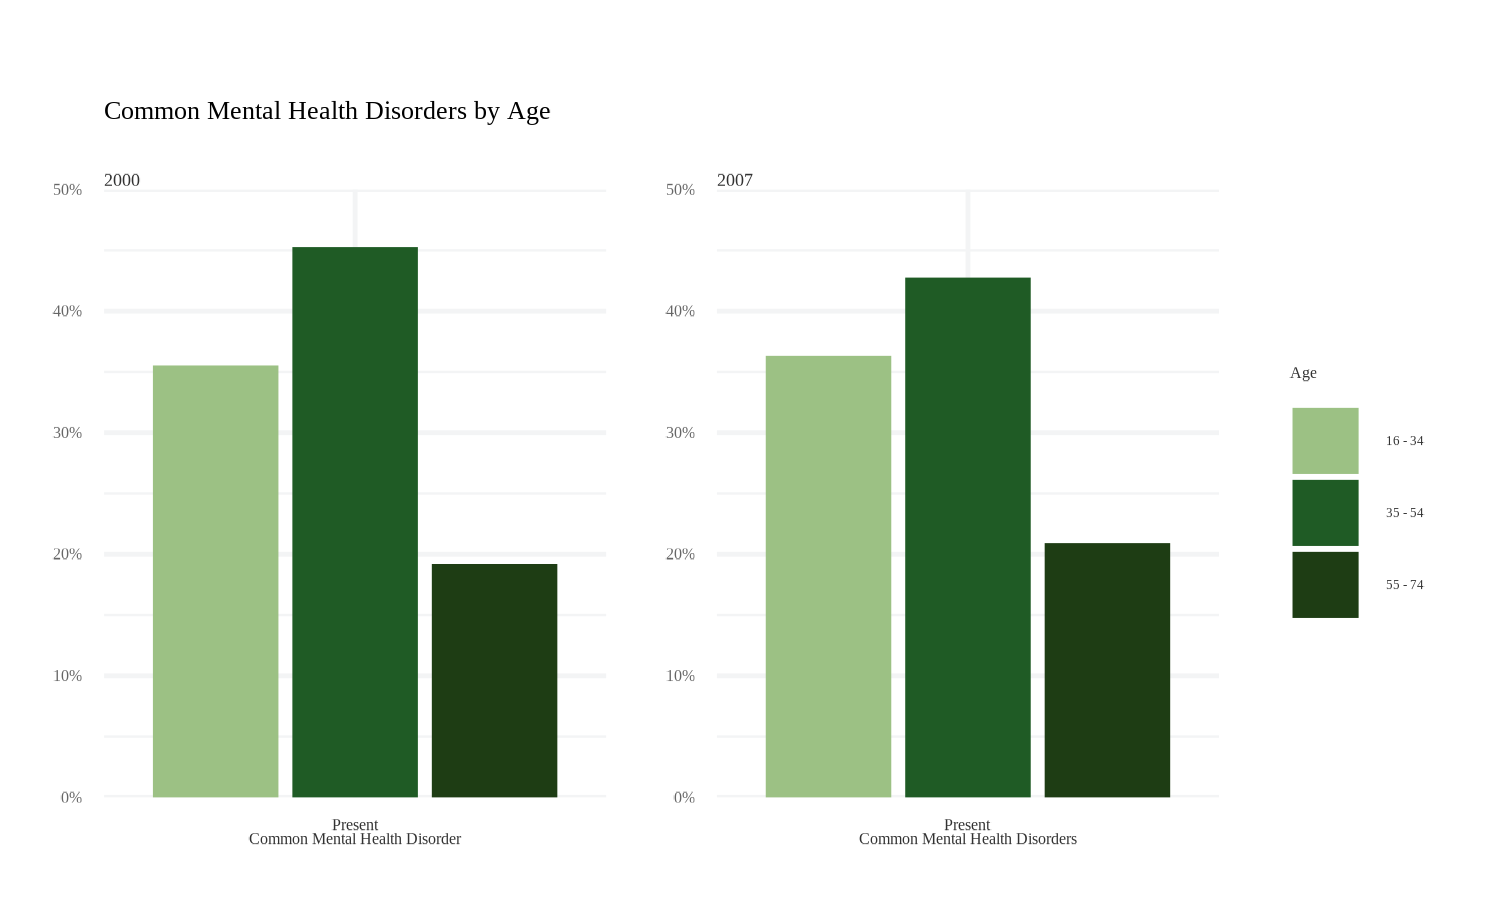
\includegraphics[width=500px,height=300px]{figure/cmd_age} \caption[Common Mental Health Disorders and Age]{Common Mental Health Disorders and Age in 2000 and 2007}\label{fig:cmdage}
\end{figure}
The data from the 2000 and 2007 survey waves reveal an interesting observation about the prevalence of common mental disorders among different age groups in the UK. Specifically, the data shows that common mental health disorders are more prevalent among younger adults (16 to 34 years old) and middle-aged adults (35 to 54 years old) compared to older adults (55 to 74 years old). In 2000, 36\% of 16- to 34-year-olds reported common mental health disorders, 45\% of 35- to 54-year-olds reported a common mental health disorder, and 13\% of 55- to 74-year-olds reported a common mental health disorder. In 2007, the trend remained consistent with 36\% of 16- to 34-year-olds reporting a common mental health disorder, 43\% of 35- to 54-year-olds reporting a common mental health disorder, and 21\% of 55- to 74-year-olds reporting a common mental health disorder.

It is important to note that these patterns of common mental health disorders prevalence may be influenced by a variety of factors such as socio-economic status, race, and gender. For example, individuals from lower socio-economic backgrounds may be more likely to experience common mental health disorders due to the stress and insecurity associated with poverty. Additionally, certain racial and ethnic groups may be disproportionately affected by mental health issues due to systemic discrimination and marginalization. Furthermore, women are more likely to be diagnosed with common mental health disorders than men and may be more likely to access mental health services for it. Therefore, it is important for any policies or programs aimed at addressing common mental health disorders to consider the potential impact of these intersecting factors.

\hypertarget{common-mental-health-disorders-and-economic-activity}{%
\subsection{Common Mental Health Disorders and Economic Activity}\label{common-mental-health-disorders-and-economic-activity}}

In 2000, of the individuals who reported living with a common mental health disorder, 63\% were economically active (in comparison with individuals who reported no common mental health disorders at 72\%), and 37\% were economically inactive (in comparison with individuals who did not have a common mental health disorder at 28\%).

In the 2007 survey wave, 40\% of individuals who reported having a common mental health disorder represented 60\% of the economically active (in comparison with those with no common mental health disorders at 71\%). For those who reported living with a common mental health disorders 40\% reported being economically inactive (in comparison with those with no common mental health disorders at 29\%) and can be seen in Table \ref{tab:results1-charcmd}.




\begin{figure}
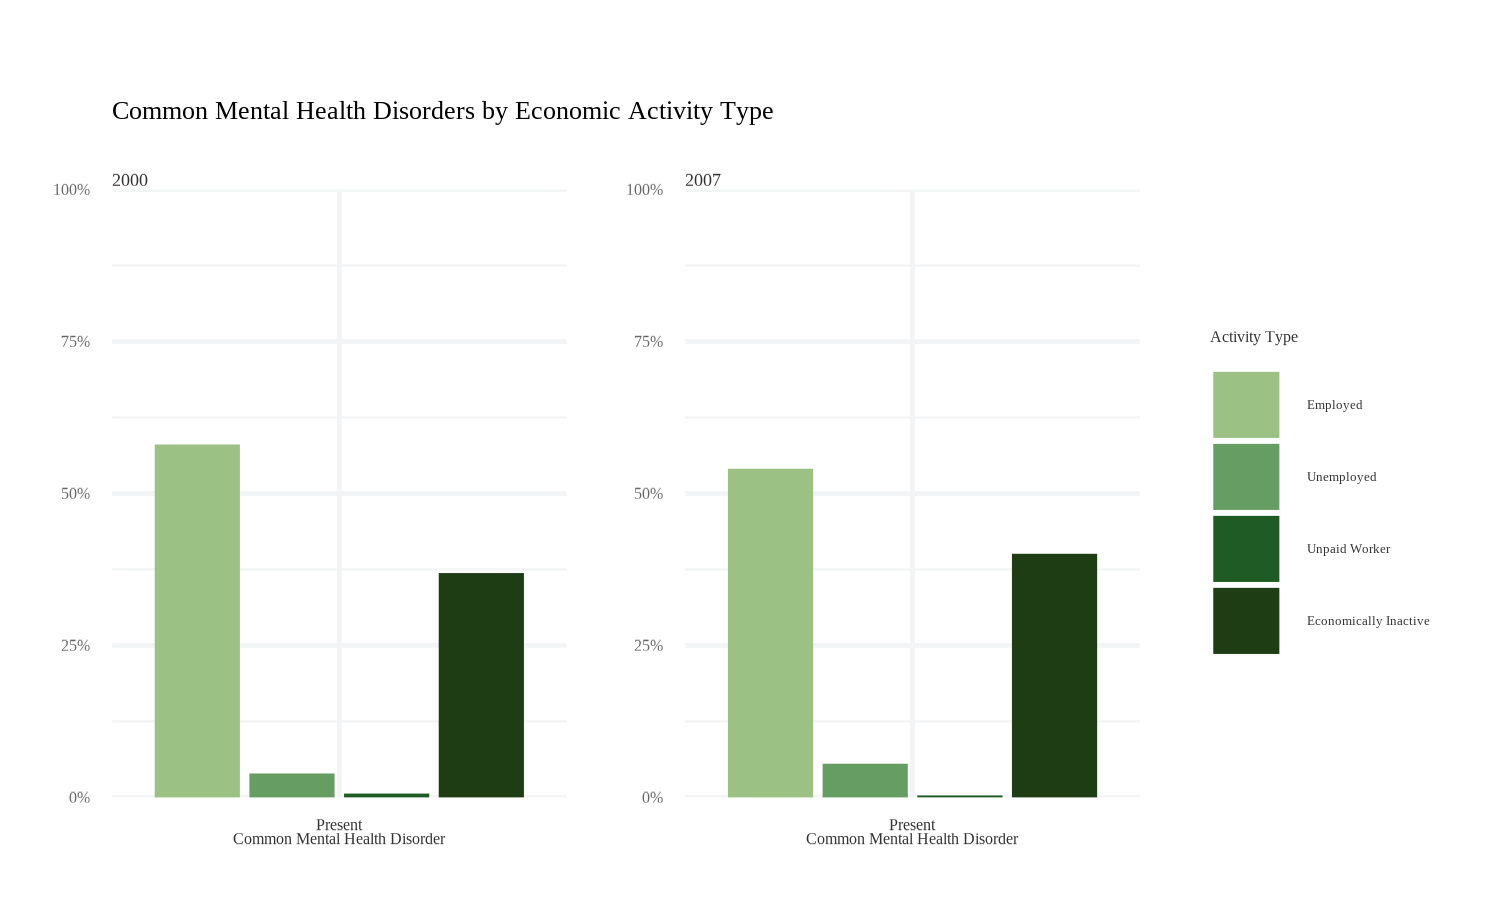
\includegraphics[width=500px,height=300px]{figure/at_cmd} \caption[Employment Status and CMD]{Employment Status and CMD in 2000 and 2007}\label{fig:cmdat}
\end{figure}
The data from the 2000 and 2007 survey waves reveal significant disparities in employment outcomes for individuals who reported living with a common mental health disorder compared to those who did not. In 2000, 58\% of individuals who reported having common mental health disorders were employed, in comparison to 69\% of individuals who did not report having a common mental health disorder. This disparity is further exacerbated among unemployed individuals, with 3.9\% of those reporting a common mental health disorder being unemployed, compared to 2.6\% of those who did not report a common mental health disorder. Similarly, unpaid workers also had a higher rate of individuals reporting a common mental health disorders, at 0.6\%, compared to 0.5\% of those who did not report a common mental health disorders.

The 2007 survey wave shows a similar pattern, with 54\% of individuals reporting a common mental health disorder being employed, in comparison to 68\% of individuals who did not report a common mental health disorder. Again, this disparity is further evident among the unemployed, with 5.5\% of those reporting a common mental health disorders being unemployed, compared to 2.7\% of those who did not report a common mental health disorders. The rate of unpaid workers remained consistent with the 2000 wave, with 0.3\% of individuals reporting a common mental health disorder and 0.3\% of individuals who did not report a common mental health disorder.

These findings highlight the need for policies and programs that address the structural barriers preventing individuals with common mental health disorders from accessing and maintaining employment. Furthermore, these findings demonstrate the need for a more comprehensive approach to mental health that addresses the intersectionality of class, race, and gender, and supports marginalized individuals in receiving the necessary support to secure and maintain employment. The fact that the majority of individuals who reported having a common mental health disorders are unemployed or unpaid workers, and the fact that the majority of individuals who did not report a common mental health disorders are employed, is a clear indication that the current mental health system is not providing individuals with the necessary support to secure stable employment.

\hypertarget{common-mental-health-disorders-and-employment-status}{%
\subsection{Common Mental Health Disorders and Employment Status}\label{common-mental-health-disorders-and-employment-status}}

Of those across both waves who indicated they lived with a common mental health disorder and were employed; the most common type of employment was full-time.




\begin{figure}
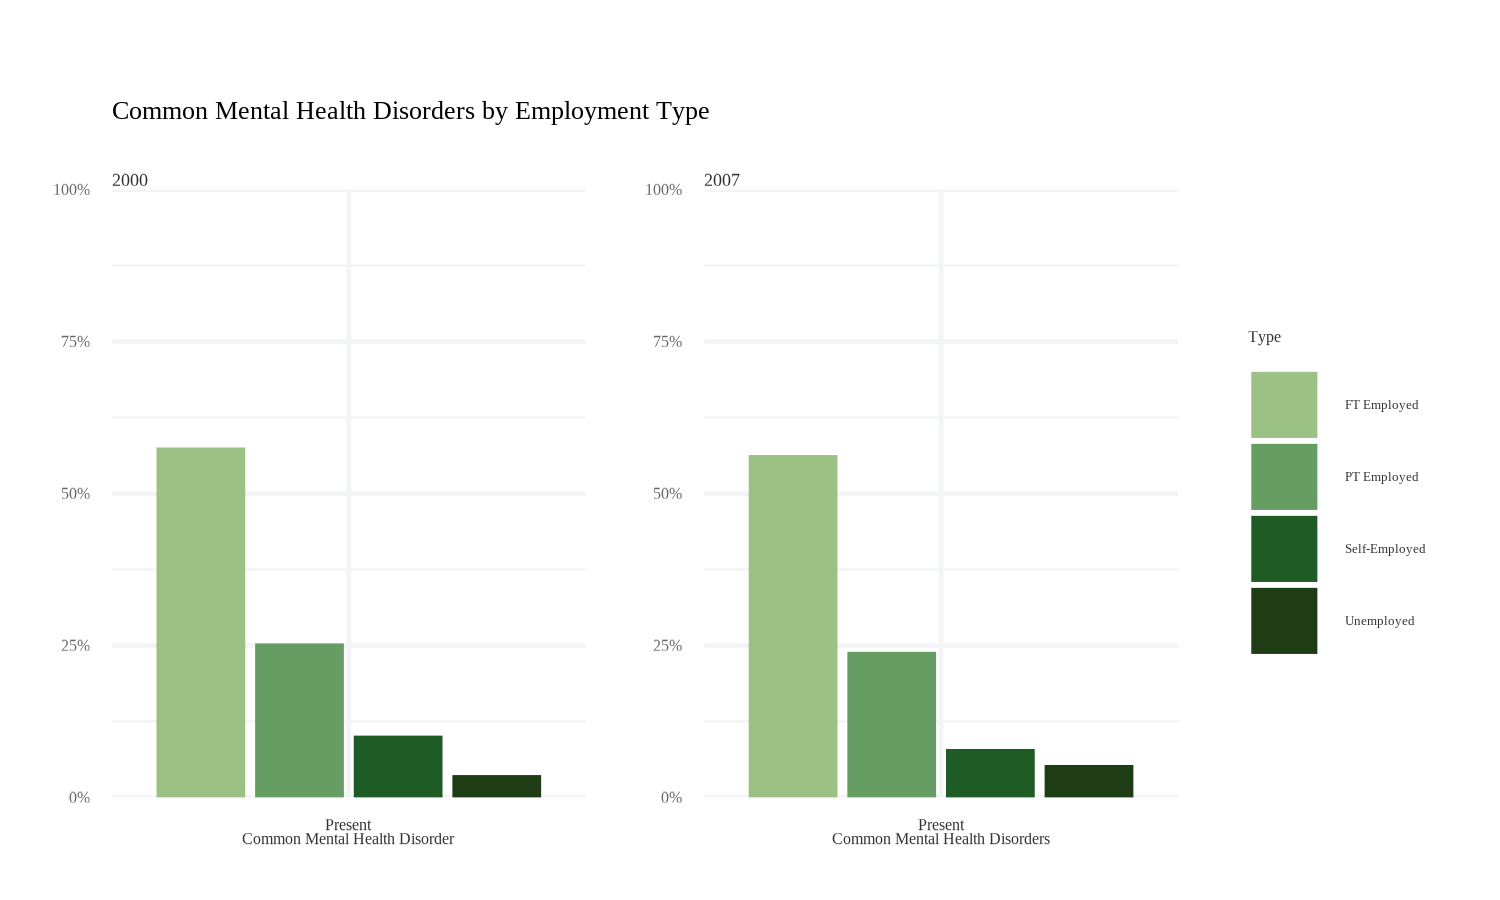
\includegraphics[width=500px,height=300px]{figure/et_cmd} \caption[Common Mental Health Disorders and Employment Type]{Common Mental Health Disorders and Employment Type in 2000 and 2007}\label{fig:cmdet}
\end{figure}
The data from the 2000 and 2007 survey waves reveal a significant disparity in labour market opportunities and outcomes for individuals who have reported a common mental disorder compared to those who have not. In the 2000 wave, the rate for full-time employed was 60\% reporting a common mental health disorder and 62\% reporting none, while for part-time employees, the rate was 26\% reporting a common mental health disorder and 24\% reporting none. For those who were self-employed the rate was 11\% reporting a common mental health disorder and 11\% reporting none. Furthermore, for those unemployed, the rate was 3.8\% reporting common mental health disorders and 2.6\% reporting none. Similarly, in the 2007 wave, the rate for full-time employees was 60\% reporting a common mental health disorder and 62\% reporting none, while for part-time employees, the rate was 26\% reporting a common mental health disorder and 23\% reporting none. For those who were self-employed the rate was 8.5\% reporting a common mental health disorder and 12\% reporting none. For those unemployed the rate was 5.7\% reporting common mental health disorders and 2.7\% reporting none.

This data reveals a clear pattern of individuals with common mental health disorders being disproportionately represented among part-time and self-employed workers, and among the unemployed, as compared to those without common mental health disorders. This highlights the need for policies and programs that address the structural barriers that prevent individuals with common mental health disorders from accessing and maintaining stable employment, particularly in full-time roles. Furthermore, these findings also demonstrate the need for a more comprehensive approach to mental health that addresses the intersectionality of class, race, and gender, and supports marginalized individuals in accessing the necessary support to secure and maintain employment. It is also important to note that the data suggests that the rate of common mental health disorders among self-employed workers decreased from 11\% in 2000 to 8.5\% in 2007, which could indicate that self-employment is not a suitable option for individuals with common mental health disorders, or that the policies and support systems in place for self-employed individuals with common mental health disorders are insufficient.

\hypertarget{type-of-common-mental-health-disorder-and-economic-activity}{%
\subsection{Type of Common Mental Health Disorder and Economic Activity}\label{type-of-common-mental-health-disorder-and-economic-activity}}

For those indicating living with a common mental health disorder within the survey waves, several different types of conditions were measured.




\begin{figure}
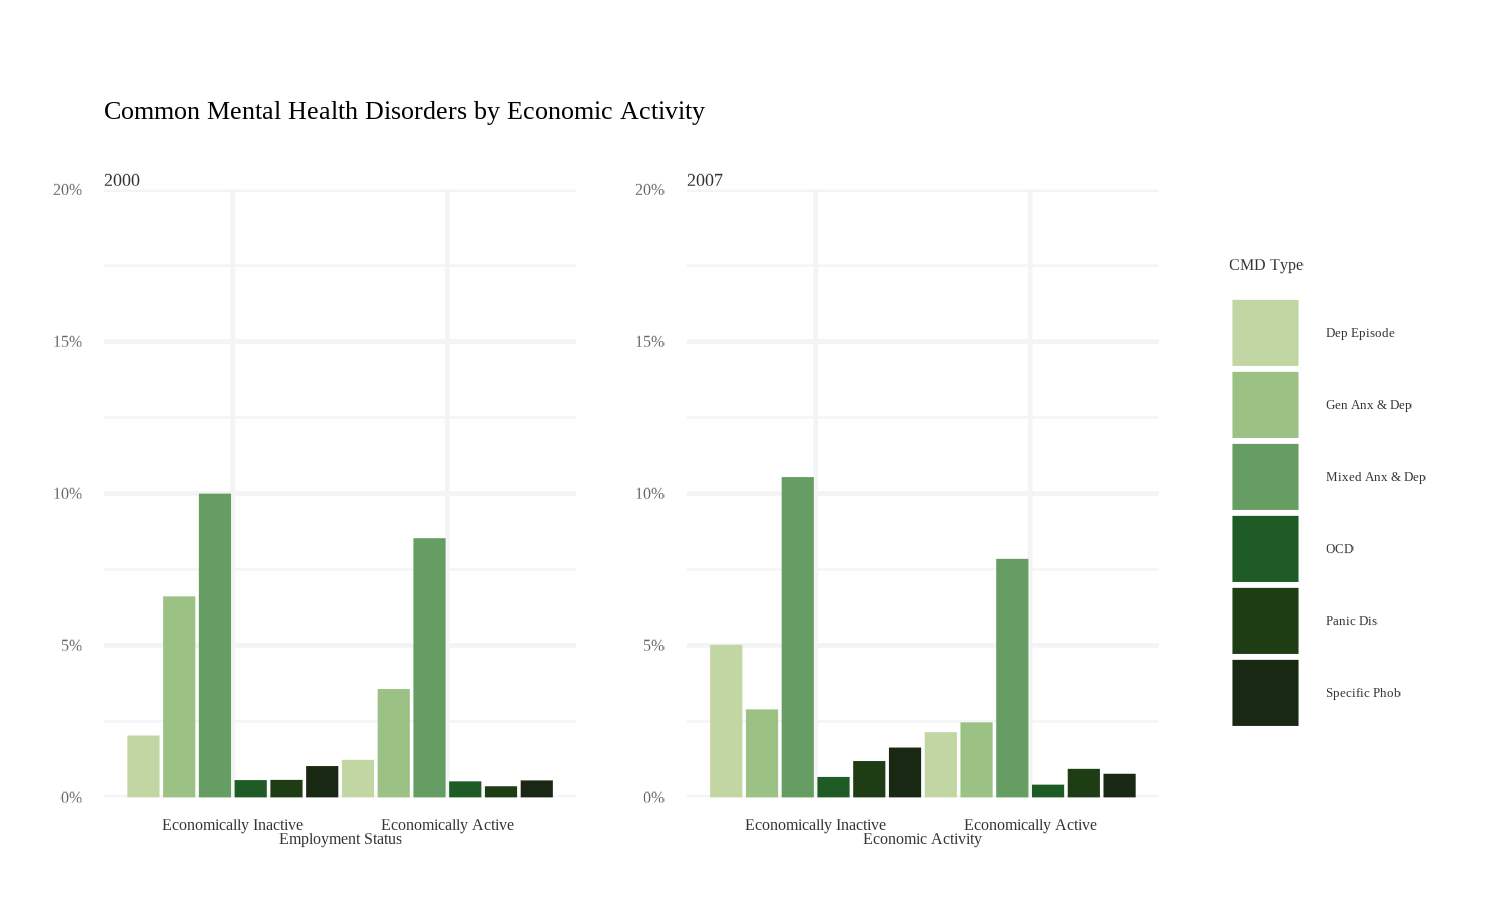
\includegraphics[width=500px,height=300px]{figure/cmdt} \caption[Common Mental Health Disorder Type and Economic Activity]{Common Mental Health Disorder Type and Economic Activity in 2000 and 2007}\label{fig:cmdt}
\end{figure}
In the 2000 survey wave, the rate of individuals reporting mixed anxiety and depression as a common mental health disorder was 58\%, with 58\% of these individuals being economically active and 42\% being economically inactive. The next highest rate was for general anxiety and depression, with 24\% of individuals reporting this as a common mental health disorder, and 24\% of these individuals being economically active and 76\% being economically inactive. The rate of individuals reporting depression as a common mental health disorder was 8.4\%, with 8.4\% of these individuals being economically active and 91.6\% being economically inactive. The rate of individuals reporting specific phobias as common mental health disorders was 3.8\%, with 3.8\% of these individuals being economically active and 96.2\% being economically inactive. The rate of individuals reporting OCD as a common mental health disorder was 3.6\%, with 3.6\% of these individuals being economically active and 96.4\% being economically inactive. Finally, the rate of individuals reporting panic disorder as a common mental health disorder was 2.5\%, with 2.5\% of these individuals being economically active and 97.5\% being economically inactive.

In the 2007 survey wave, the rate of individuals reporting mixed anxiety and depression as a common mental health disorder was 54\%, with 54\% of these individuals being economically active and 46\% being economically inactive. The rate of individuals reporting depression as a common mental health disorder was 15\%, with 15\% of these individuals being economically active and 85\% being economically inactive. The rate of individuals reporting general anxiety and depression as a common mental health disorder was 17\%, with 17\% of these individuals being economically active and 83\% being economically inactive. The rate of individuals reporting specific phobias as a common mental health disorder was 5.3\%, with 5.3\% of these individuals being economically active and 94.7\% being economically inactive. The rate of individuals reporting panic disorder as a common mental health disorder was 6.4\%, with 6.4\% of these individuals being economically active and 93.6\% being economically inactive. Finally, the rate of individuals reporting OCD as a common mental health disorder was 2.9\%, with 2.9\% of these individuals being economically active and 97.1\% being economically inactive.

The data from the 2000 and 2007 survey waves reveal a significant disparity in labour market opportunities and outcomes for individuals living with a common mental disorder compared to those without. The fact that a majority of individuals living with common mental health disorders are economically inactive, while the majority of individuals who do not have a common mental health disorders are economically active, is a clear indication that the current mental health system is not providing individuals with the necessary support to secure stable employment.

\hypertarget{common-mental-health-disorder-and-reason-for-economic-inactivity}{%
\subsection{Common Mental Health Disorder and Reason for Economic Inactivity}\label{common-mental-health-disorder-and-reason-for-economic-inactivity}}

In the 2000 survey wave, 29\% of individuals who were economically inactive reported that their inactivity was due to a physical health problem, 9.8\% reported that it was due to a mental health problem, 22\% reported that there was no suitable job available, and 39\% reported that they did not need or want a job.
Similarly, in the 2007 survey wave, 32\% of economically inactive individuals cited a physical health problem as the reason for their inactivity, 10\% cited a mental health problem, 21\% cited no suitable job available, and 37\% reported not needing or wanting a job.




\begin{figure}
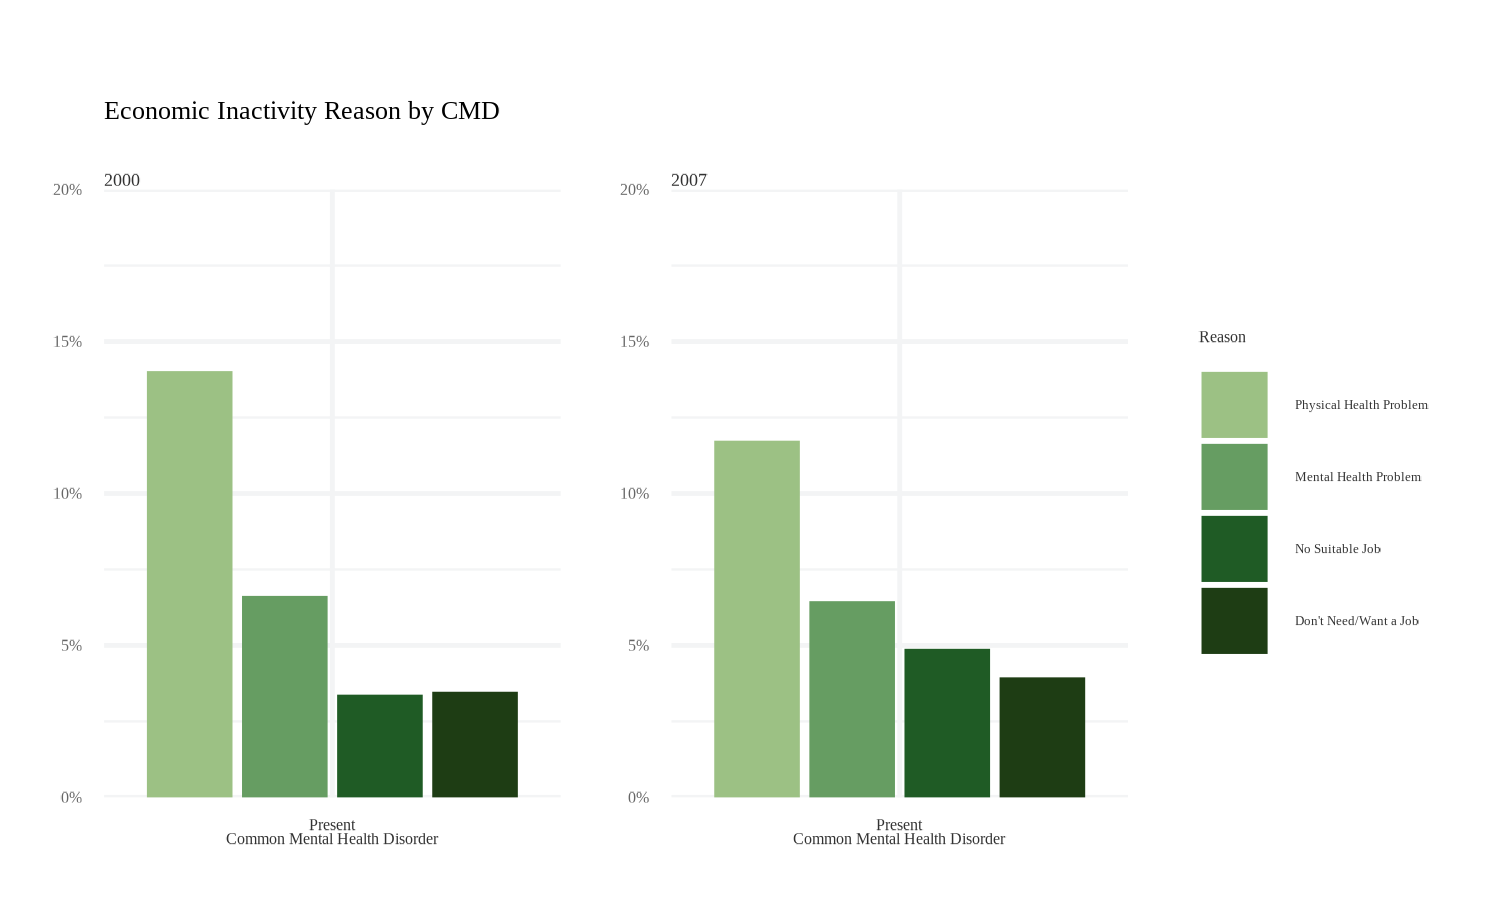
\includegraphics[width=500px,height=300px]{figure/cmdir} \caption[Reasons for Economic Inactivity and CMD]{Reasons for Economic Inactivity and CMD in 2000 and 2007}\label{fig:cmdir}
\end{figure}
For the 2000 survey wave, for those who were inactive and indicated as also living with any type of common mental health disorders, 51\% indicated that having a physical health problem was the reason (for those with no common mental health disorders it was 23\%). 24\% indicated a mental health problem as the reason alongside living with a common mental health disorder (3.1\% for those with no common mental health disorders). Not being able to find a suitable job accounted for 12\% for those with common mental health disorders (and 25\% without). For those with a common mental health disorder, not wanting or needing a job was 13\% (and 49\% who had no common mental health disorders).

Similarly, in the 2007 survey wave, for those who were inactive and indicated as also living with any type of common mental health disorders, 43\% indicated that having a physical health problem was the reason (for those with no common mental health disorders it was 12\%). 24\% indicated a mental health problem as the reason alongside living with a common mental health disorder (2.3\% for those with no common mental health disorders). Not being able to find a suitable job accounted for 18\% for those with common mental health disorders (and 24\% without). For those with a common mental health disorder, not wanting or needing a job was 15\% (and 52\% who had no common mental health disorders).

Interestingly, individuals living with a common mental health disorders and being economically inactive have a higher percentage indicating that a physical health problem is the reason for their inactivity, compared to those without a common mental health disorders. In the 2000 survey wave, 51\% of those with a common mental health disorders cited a physical health problem as the reason for inactivity, compared to 23\% of those without a common mental health disorders. Similarly, in the 2007 survey wave, 43\% of those with a common mental health disorder cited a physical health problem as the reason for inactivity, compared to 12\% of those without a common mental health disorder. This highlights the intersectional nature of disabilities and the impact of physical health on the ability to secure and maintain employment for those living with common mental health disorders. The fact that a significant proportion of the individuals who have a common mental health disorders are economically inactive and that the reasons for inactivity are not just limited to the mental health condition itself, but also due to lack of suitable job opportunities and discrimination in the labour market, is a clear indication of the systemic barriers that individuals with common mental health disorders face in the workforce.

\hypertarget{common-mental-health-disorders-and-education}{%
\subsection{Common Mental Health Disorders and Education}\label{common-mental-health-disorders-and-education}}

In the 2000 survey wave, the overall rate for having no qualifications was 27\%, 51\% for GCSE's and A Levels and equivalent and 22\% for degrees. In 2007, overall, 23\% of individuals reported having no qualifications, 47\% reported having GCSE's and A Levels and their equivalent, and 30\% reported having an undergraduate degree as their highest educational qualification.




\begin{figure}
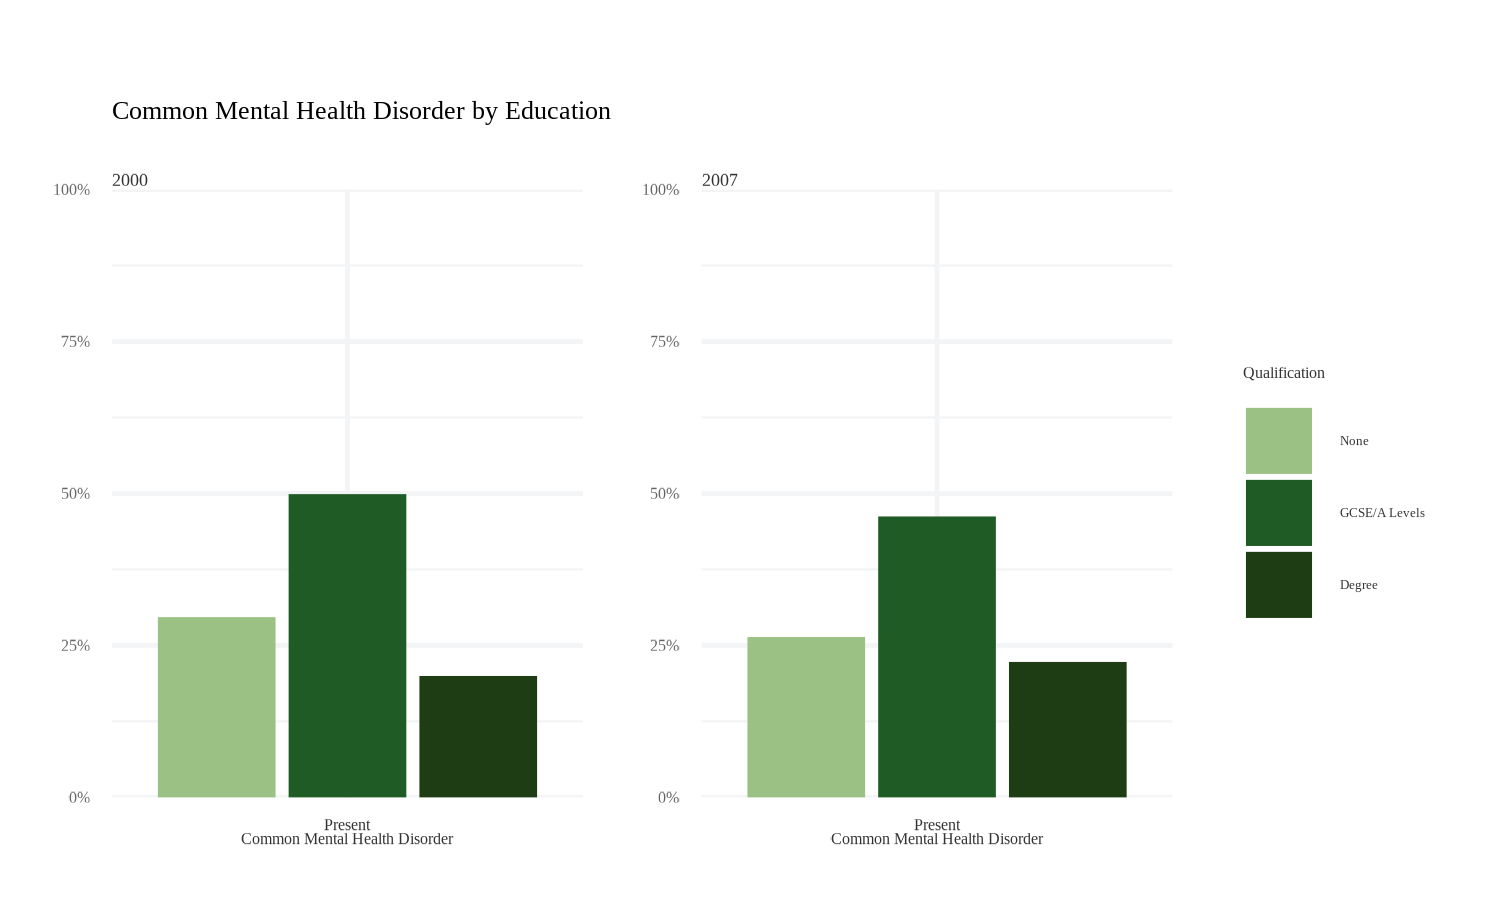
\includegraphics[width=500px,height=300px]{figure/cmded} \caption[Common Mental Health Disorder and Education]{Common Mental Health Disorder and Education in 2000 and 2007}\label{fig:cmded}
\end{figure}
In the 2000 survey wave, data reveals that individuals living with a common mental health disorder had a 30\% rate of having no qualifications, compared to those without a common mental health disorder at 26\%. Additionally, 50\% of individuals living with a common mental health disorder had gained their GCSEs or A Levels, compared to 52\% without a common mental health disorders, and 20\% of those living with a common mental health disorders had gained an undergraduate degree, compared to 22\% without a common mental health disorders.

In the 2007 survey wave, the trend continues with 28\% of individuals living with a common mental health disorder having no qualifications, compared to those without a common mental health disorder at 22\%. Additionally, 49\% of individuals living with a common mental health disorders had gained their GCSEs or A Levels, compared to 47\% without a common mental health disorders, and 23\% of those living with a common mental health disorders had gained an undergraduate degree, compared to 31\% without a common mental health disorders.

These findings highlight the structural barriers that individuals living with a common mental health disorders face in accessing and completing higher education, and the need for policies and programs that address these disparities. Additionally, it is important to note that these disparities are not limited to just those with a common mental health disorders, but to marginalized individuals across the intersectionality of class, race, and gender.

Hypothesis testing found that there was not a statistically significant relationship between having a common mental health disorders and educational qualification for the 2000 survey wave, but that there was a significant relationship for those in the 2007 survey wave (Table \ref{tab:results1-charcmd}).

One interesting similarity between the 2000 and 2007 survey waves is that the most common educational qualification for those who reported living with a common mental health disorder is GCSEs or their equivalent. Another similarity is that the rate of those with no qualifications is higher among those with a common mental health disorder compared to those without.

An interesting difference between the two survey waves is that in 2000 there was not a statistically significant relationship between having a common mental health disorder and educational qualification, while in 2007 there was a significant relationship. Additionally, in 2007 there was a higher percentage of those who have gained an undergraduate degree among those with no common mental health disorders, compared to those with a common mental health disorders.

\hypertarget{common-mental-health-disorders-and-social-class}{%
\subsection{Common Mental Health Disorders and Social Class}\label{common-mental-health-disorders-and-social-class}}

In the 2000 and 2007 survey waves, there were notable differences between the proportion of individuals with common mental health disorders and those without in terms of their social class status. The data reveals that a higher proportion of individuals with common mental health disorders were found in the skilled class (93\% in 2000 and 94\% in 2007) while a lower proportion were found in the unskilled class (6.9\% in 2000 and 6\% in 2007) compared to individuals without common mental health disorders. These findings suggest that individuals with common mental health disorders may face additional barriers to social mobility and economic stability.




\begin{figure}
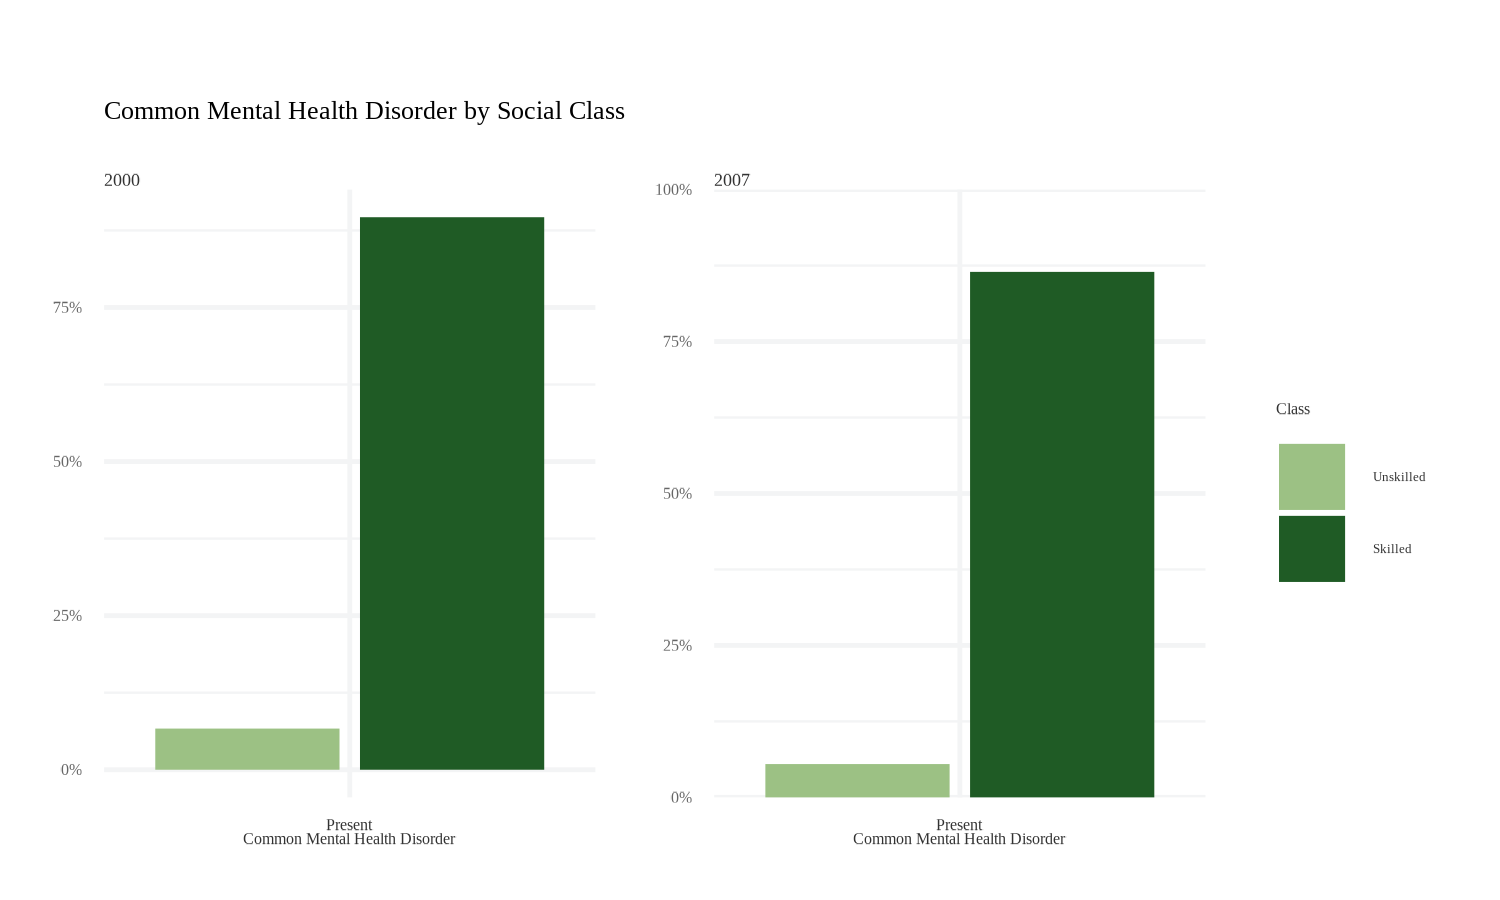
\includegraphics[width=500px,height=300px]{figure/cmdsc} \caption[Common Mental Health Disorders and Social Class]{Common Mental Health Disorders and Social Class in 2000 and 2007}\label{fig:cmdsc}
\end{figure}
The data from the 2000 and 2007 survey waves suggests a significant relationship between the presence of common mental health disorders and social class. Specifically, the data shows that individuals who reported living with common mental health disorders were disproportionately represented in the unskilled class, with 6.9\% in 2000 (compared to 5.5\% without a common mental health disorders) and 6\% in 2007 (compared to 4.3\% without a common mental health disorders). An interesting observation is that the percentage of individuals who reported living with a common mental health disorder in the unskilled class is relatively low in both the 2000 and 2007 survey waves (6.9\% and 6\% respectively) when compared to those in the skilled class (93\% and 94\% respectively). Additionally, there is a significant relationship between the presence of a common mental health disorder and social class for those in the 2000 and 2007 survey waves. This suggests that individuals in higher social class may have better access to resources and support that could help them manage their common mental health disorders, while individuals in lower social class may face more barriers to getting help and support for their common mental health disorders.

Hypothesis testing found that there was a significant relationship between the presence of a common mental health disorder and social class for those in the 2007 survey wave only (Table \ref{tab:results1-charcmd}).

\hypertarget{common-mental-health-disorders-and-ethnicity}{%
\subsection{Common Mental Health Disorders and Ethnicity}\label{common-mental-health-disorders-and-ethnicity}}

The data from the 2000 and 2007 survey waves reveal a significant majority of individuals indicating they were of white ethnicity, with 93\% in 2000 and 89\% in 2007. However, it is important to note that a non-trivial percentage of individuals, 7.4\% in 2000 and 11\% in 2007, indicated that they were of another ethnicity.




\begin{figure}
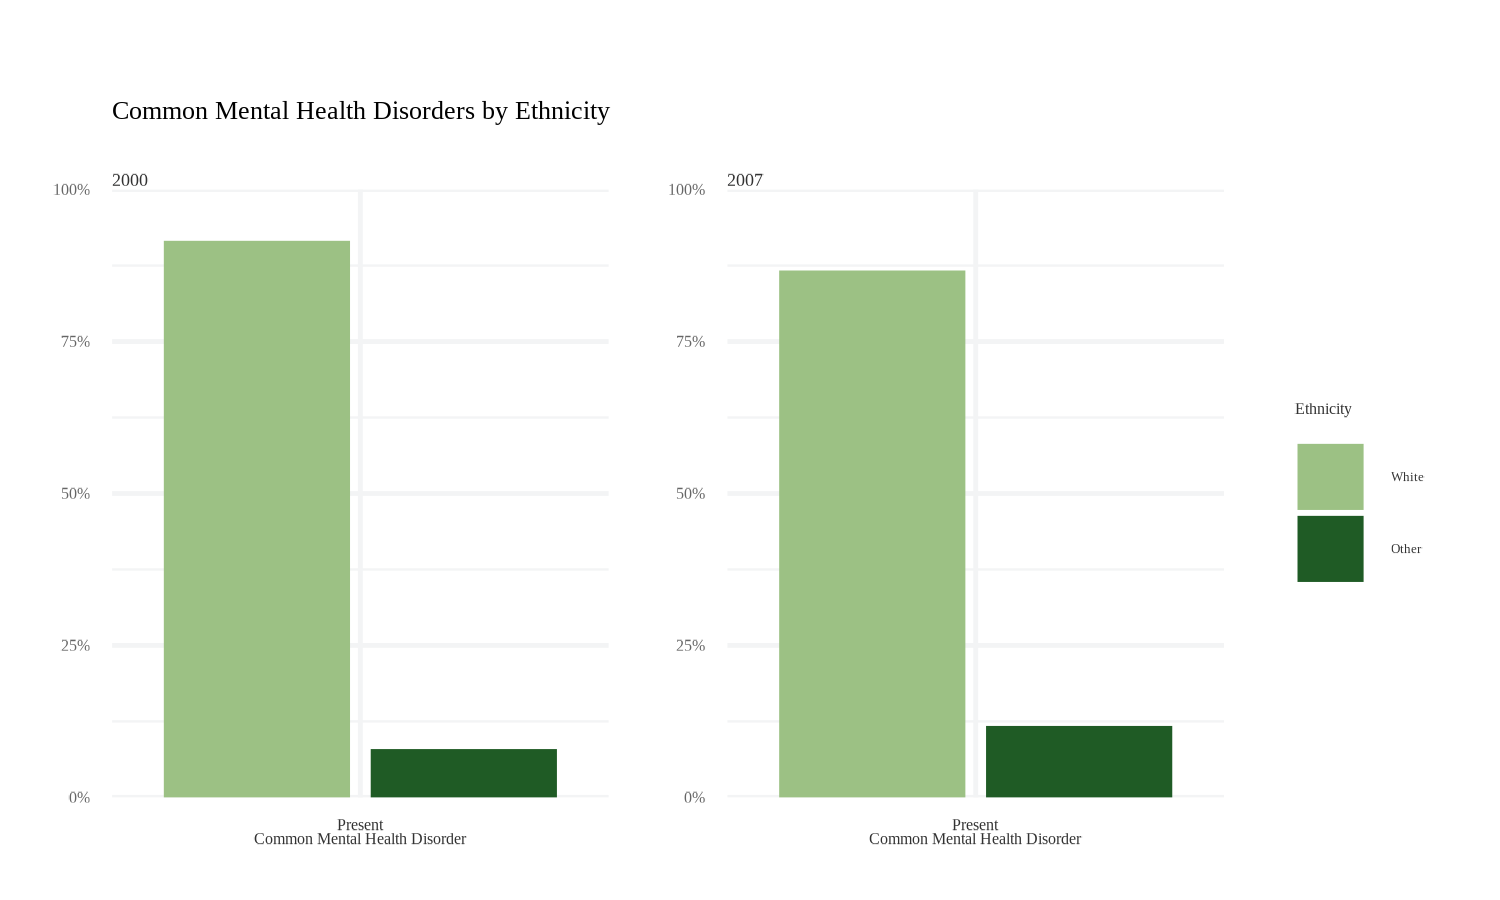
\includegraphics[width=500px,height=300px]{figure/cmdeth} \caption[Common Mental Health Disorders and Ethnicity]{Common Mental Health Disorders and Ethnicity in 2000 and 2007}\label{fig:cmdeth}
\end{figure}
In the 2000 and 2007 survey waves, there were disparities in the representation of ethnic minorities among individuals who reported living with a common mental health disorder. In both waves, a higher proportion of white individuals reported living with a common mental health disorder, with 92\% in 2000 and 93\% in 2007, compared to individuals of other ethnicities at 8\% and 12\% respectively. These findings raise important questions about the impact of structural racism and discrimination on access to mental health services and support for marginalized communities. Hypothesis testing did not find a significant relationship between the presence of common mental health disorders and ethnicity in the 2000 or 2007 survey waves, further emphasizing the need for further research and examination of the intersections of race, class, and mental health.

An interesting observation from the last answer is that there is not a significant difference in the proportion of individuals with a common mental health disorder who identify as white versus those who identify as a minority ethnicity in the 2000 and 2007 survey waves. This suggests that the prevalence of common mental health disorders may not be disproportionately affecting any one particular ethnic group, but it is important to note that this may be due to the limited sample size of ethnic minorities in the survey and further research is needed to fully understand the relationship between common mental health disorders and ethnicity.
Hypothesis testing did not find a significant relationship between the presence of common mental health disorders and ethnicity in the 2000 or 2007 survey waves.

\hypertarget{common-mental-health-disorders-and-physical-health}{%
\subsection{Common Mental Health Disorders and Physical Health}\label{common-mental-health-disorders-and-physical-health}}

The data from the 2000 and 2007 survey waves had the same overall rates and reveal that a significant portion of the population, 18\%, reported having a physical health condition. This is a notable finding as it highlights the prevalence of physical health issues among the population and the potential impact it may have on individuals' daily lives. Furthermore, it is important to note that the rates of physical health conditions were consistent across both survey waves, indicating that this is a persistent issue that requires attention.




\begin{figure}
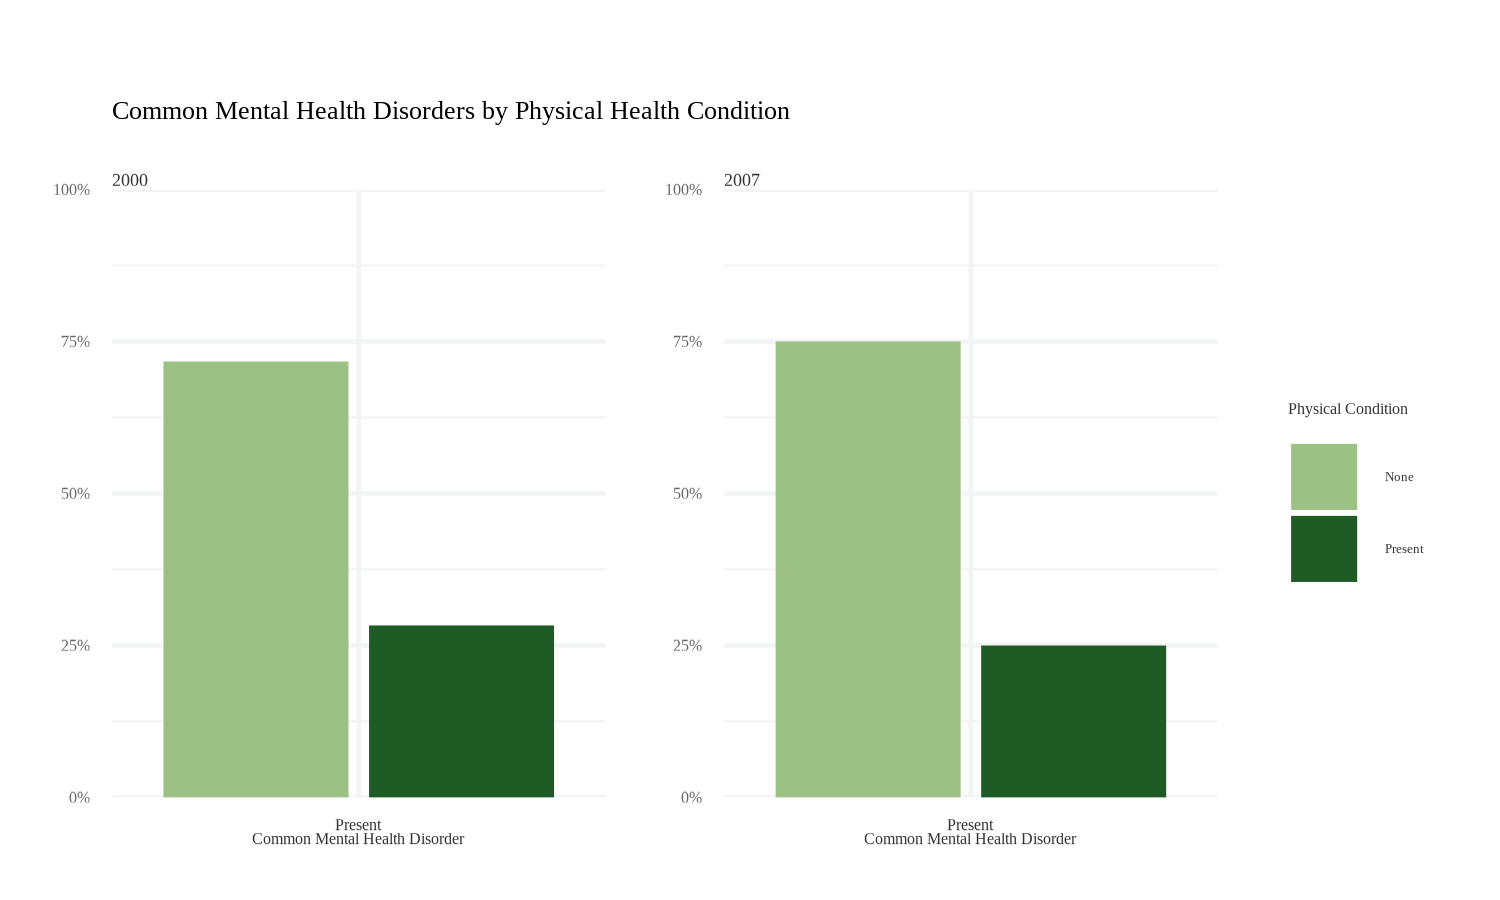
\includegraphics[width=500px,height=300px]{figure/cmdphc} \caption[Common Mental Health Disorders and Physical Health Condition]{Common Mental Health Disorders and Physical Health Condition in 2000 and 2007}\label{fig:cmdphc}
\end{figure}
The data from the 2000 and 2007 survey waves reveal a significant relationship between the presence of common mental health disorders and physical health conditions. In the 2000 survey, 28\% (of those with common mental health disorders) reported having a physical health condition, and 72\% (of those with common mental health disorders) reported having no physical health condition (compared to 16\% and 84\%, respectively, of those without common mental health disorders). Similarly, in the 2007 survey, 25\% (of those with common mental health disorders) reported having a physical health condition, and 75\% (of those with common mental health disorders) reported having no physical health conditions (compared to 16\% and 84\%, respectively, of those without common mental health disorders). These findings demonstrate the need for a more comprehensive approach to healthcare that addresses the social determinants of health, such as class, race, and gender, and supports marginalized individuals in receiving the necessary support for both their physical and mental health. The fact that a higher proportion of individuals living with a common mental health disorder also reported a physical health condition is an indication that the current healthcare system is not providing individuals with the necessary support to manage both their mental and physical health.

An interesting observation from the last answer is that there is a higher percentage of individuals living with a common mental health disorder who also report having a physical health condition, compared to individuals without a common mental health disorder. This highlights the potential for individuals living with a common mental health disorder to have a greater burden of physical health issues, and the need for healthcare providers to address this intersectionality when providing care.

Hypothesis testing also found a significant relationship between presence of common mental health disorders and presence of a physical health condition in both the 2000 and 2007 survey waves.

\hypertarget{common-mental-health-disorders-and-treatment-use}{%
\subsection{Common Mental Health Disorders and Treatment Use}\label{common-mental-health-disorders-and-treatment-use}}

The most common form of mental health treatment in both survey waves was none at all, and the least common being counselling or therapy only. In 2000 the overall rates are 93\% for none, 4.6\% were medication only, 1.2\% for counselling only, and 1.1\% for both. In 2007 the overall rates are 93\% for none, 4.7\% were medication only, 1.6\% for counselling only, and 1.2\% for both.




\begin{figure}
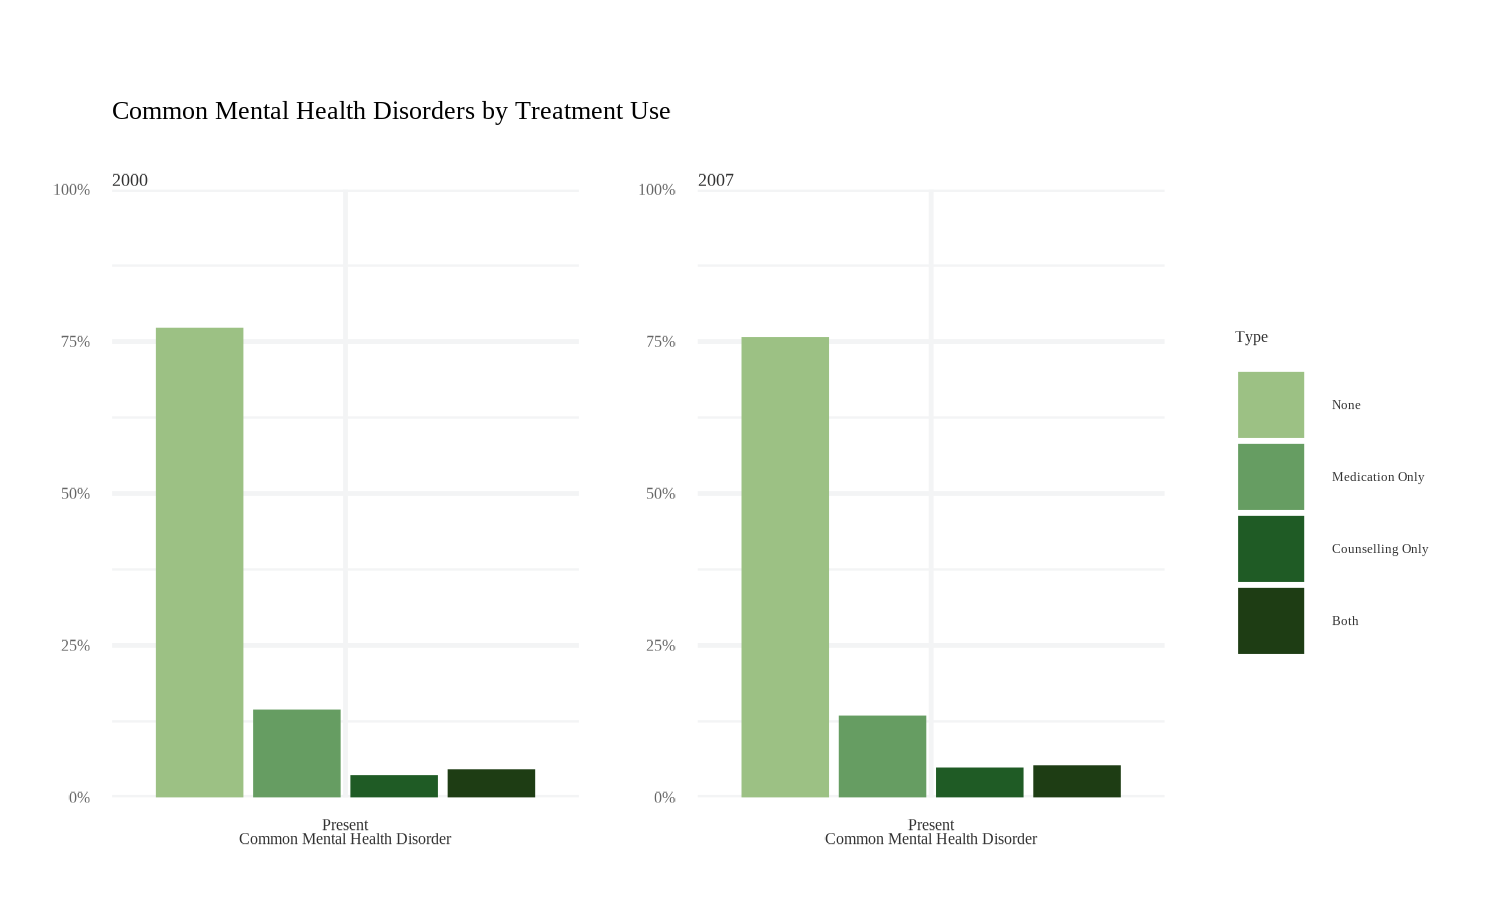
\includegraphics[width=500px,height=300px]{figure/cmdtrt} \caption[Common Mental Health Disorders and Treatment Use]{Common Mental Health Disorders and Treatment Use in 2000 and 2007}\label{fig:cmdtrt}
\end{figure}
In the 2000 survey wave, 93\% of individuals who reported living with a common mental health disorders did not take part in any mental health treatment (compared to 96\% of those with no common mental health disorders), 4.6\% took medication only (compared to 2.7\% with no common mental health disorders), 1.2\% took counselling or therapy only (compared to 0.8\% with no common mental health disorders), and 1.1\% took both medication and counseling or therapy (compared to 0.4\% with no common mental health disorders).

In the 2007 survey wave, 93\% of individuals who reported living with a common mental health disorders did not take part in any mental health treatment (compared to 96\% of those with no common mental health disorders), 4.7\% took medication only (compared to 2.9\% with no common mental health disorders), 1.6\% took counseling or therapy only (compared to 0.9\% with no common mental health disorders), and 1.2\% took both medication and counseling or therapy (compared to 0.4\% with no common mental health disorders).

The data suggests a clear pattern of individuals living with common mental health disorders having limited access to mental health treatment options in the UK. The majority of individuals in both survey waves, whether they have a common mental health disorder or not, did not receive any form of mental health treatment. Furthermore, the data shows that individuals living with common mental health disorders are disproportionately represented among those who only receive medication as a form of treatment and underrepresented among those who receive both medication and counseling or therapy, or counseling or therapy alone. This suggests that individuals living with common mental health disorders in the UK may be facing systemic barriers to accessing more comprehensive and effective forms of mental health treatment, or treatments that help remove the need for medication; examine social and structural barriers to good mental health. This highlights the need for a more equitable and inclusive mental health care system that addresses these disparities and ensures that all individuals living with common mental health disorders have access to the treatment they need.

Hypothesis testing also found a significant relationship between presence of a common mental health disorder and presence of a physical health condition in both the 2000 and 2007 survey waves.

\hypertarget{common-mental-health-disorders-and-mental-health-services}{%
\subsection{Common Mental Health Disorders and Mental Health Services}\label{common-mental-health-disorders-and-mental-health-services}}

Engaging with mental health services was derived from individuals reporting that they had received health care for a mental health condition, including their GP, inpatient and outpatient hospital appointments and community mental health teams. In 2000 the overall rate for having not used any services was 88\% and having used services at 12\%. In 2007 the overall rates were the same.




\begin{figure}
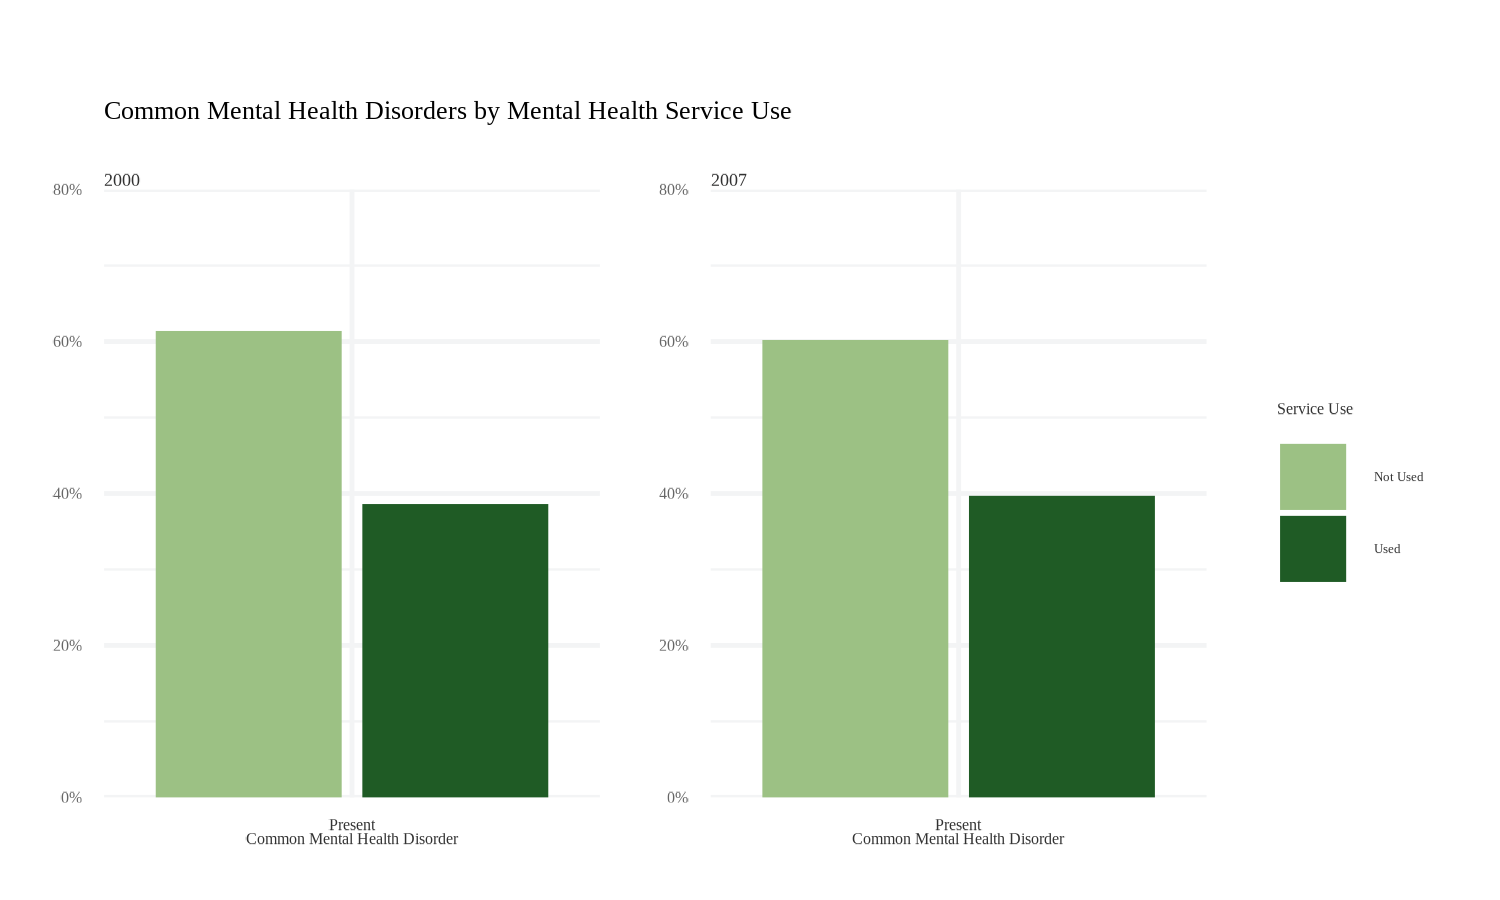
\includegraphics[width=500px,height=300px]{figure/cmdsu} \caption[Common Mental Health Disorders and Mental Health Service Use]{Common Mental Health Disorders and Mental Health Service Use 2000 and 2007}\label{fig:cmdsu}
\end{figure}
In the 2000 and 2007 survey waves, it is clear that there is a significant disparity in the access and utilization of mental health services among individuals who reported living with a common mental health disorder compared to those who reported no common mental health disorders. Specifically, 61\% and 60\% of individuals who reported not using any mental health services also reported living with a common mental health disorder, while only 39\% and 40\% of individuals who reported using mental health services also reported living with a common mental health disorder. This suggests that individuals living with common mental health disorders are less likely to access and utilize mental health services, a concerning phenomenon that highlights the systemic barriers and discrimination faced by individuals living with a common mental health disorders in the UK's mental health system during this time period. This is further reinforced by the fact that 94\% of those who did not use mental health services reported no common mental health disorders, and only 6.5\% and 6.1\% of those who did use mental health services reported no common mental health disorders. This implies that individuals with common mental health disorders were less likely to receive the support they needed and were more likely to be left untreated during this time period.

An interesting observation is that in both the 2000 and 2007 survey waves, a large majority of individuals who reported not using any mental health services also reported living with a common mental health disorders, and a small percentage of those who reported using mental health services also reported living with a common mental health disorders. This could suggest that despite the high rates of common mental health disorders present in the population, a significant number of individuals are not accessing or utilizing mental health services, which could be due to barriers such as lack of knowledge, stigma, or lack of accessibility to services. This highlights the need for more effective mental health outreach and support for individuals living with common mental health disorders, particularly for those who are not accessing traditional mental health services. This highlights the importance of addressing systemic issues that may be preventing individuals living with a common mental health disorder from accessing mental health services. This could include financial barriers, lack of knowledge about available resources, discrimination and stigma surrounding mental health, and a lack of culturally sensitive and appropriate mental health services. Additionally, there is a need for mental health professionals to actively reach out to and engage marginalized communities, rather than relying on them to seek help on their own.

It is also important to note that the high rate of individuals living with common mental health disorders who did not use mental health services may also reflect the quality and effectiveness of the mental health services available. The data suggests that mental health services in the UK between 2000 and 2007 might not have been effective enough to keep individuals living with common mental health disorders engaged and motivated to continue treatment.

Hypothesis testing found a significant relationship between using any mental health service and a common mental health disorder being present in both the 2000 and 2007 survey waves.

\hypertarget{severe-mental-illness-2}{%
\section{Severe Mental Illness}\label{severe-mental-illness-2}}

\hypertarget{sample-overview-1}{%
\subsection{Sample Overview}\label{sample-overview-1}}

The table below serves as a summary and the section will delve deeper into specific values and trends for a more complete and holistic understanding of the data and its implications. Breaking the survey waves down by severe mental illness presence shows statistically significant relationships in the majority of variables (Table \ref{tab:results1-charsmi}).

\providecommand{\huxb}[2]{\arrayrulecolor[RGB]{#1}\global\arrayrulewidth=#2pt}
  \providecommand{\huxvb}[2]{\color[RGB]{#1}\vrule width #2pt}
  \providecommand{\huxtpad}[1]{\rule{0pt}{#1}}
  \providecommand{\huxbpad}[1]{\rule[-#1]{0pt}{#1}}
\begin{table}[ht]
\begin{centerbox}
\begin{threeparttable}
 \setlength{\tabcolsep}{0pt}
\begin{adjustbox}{width=1\textwidth}
\large
\begin{tabular}{l l l l l l l l l l l}


\hhline{>{\arrayrulecolor[RGB]{0, 0, 0}\global\arrayrulewidth=0.4pt}->{\arrayrulecolor[RGB]{0, 0, 0}\global\arrayrulewidth=0.4pt}->{\arrayrulecolor[RGB]{0, 0, 0}\global\arrayrulewidth=0.4pt}->{\arrayrulecolor[RGB]{0, 0, 0}\global\arrayrulewidth=0.4pt}->{\arrayrulecolor[RGB]{0, 0, 0}\global\arrayrulewidth=0.4pt}->{\arrayrulecolor[RGB]{0, 0, 0}\global\arrayrulewidth=0.4pt}->{\arrayrulecolor[RGB]{0, 0, 0}\global\arrayrulewidth=0.4pt}->{\arrayrulecolor[RGB]{0, 0, 0}\global\arrayrulewidth=0.4pt}->{\arrayrulecolor[RGB]{0, 0, 0}\global\arrayrulewidth=0.4pt}->{\arrayrulecolor[RGB]{0, 0, 0}\global\arrayrulewidth=0.4pt}->{\arrayrulecolor[RGB]{0, 0, 0}\global\arrayrulewidth=0.4pt}-}
\arrayrulecolor{black}

\multicolumn{1}{!{\color[RGB]{0, 0, 0}\vrule width 0pt}l!{\color[RGB]{0, 0, 0}\vrule width 0pt}}{\rule{0pt}{1pt + 1em}\raggedright \hspace{0pt} \textbf{{\fontsize{14pt}{16.8pt}\selectfont 
}} \hspace{1pt}\rule[-1pt]{0pt}{1pt}} &
\multicolumn{5}{c!{\color[RGB]{0, 0, 0}\vrule width 0pt}}{\rule{0pt}{1pt + 1em}\centering \hspace{1pt} \textbf{{\fontsize{14pt}{16.8pt}\selectfont \textbf{2000 Wave}
}} \hspace{1pt}\rule[-1pt]{0pt}{1pt}} &
\multicolumn{5}{c!{\color[RGB]{0, 0, 0}\vrule width 0pt}}{\rule{0pt}{1pt + 1em}\centering \hspace{1pt} \textbf{{\fontsize{14pt}{16.8pt}\selectfont \textbf{2007 Wave}
}} \hspace{1pt}\rule[-1pt]{0pt}{1pt}} \tabularnewline[-0.5pt]


\hhline{}
\arrayrulecolor{black}

\multicolumn{1}{!{\color[RGB]{0, 0, 0}\vrule width 0pt}l!{\color[RGB]{0, 0, 0}\vrule width 0pt}}{\rule{0pt}{1pt + 1em}\raggedright \hspace{0pt} \textbf{{\fontsize{14pt}{16.8pt}\selectfont \textbf{Characteristic}
}} \hspace{1pt}\rule[-1pt]{0pt}{1pt}} &
\multicolumn{1}{c!{\color[RGB]{0, 0, 0}\vrule width 0pt}}{\rule{0pt}{1pt + 1em}\centering \hspace{1pt} \textbf{{\fontsize{14pt}{16.8pt}\selectfont \textbf{N}
}} \hspace{1pt}\rule[-1pt]{0pt}{1pt}} &
\multicolumn{1}{c!{\color[RGB]{0, 0, 0}\vrule width 0pt}}{\rule{0pt}{1pt + 1em}\centering \hspace{1pt} \textbf{{\fontsize{14pt}{16.8pt}\selectfont \textbf{Overall}, N = 7,247
}} \hspace{1pt}\rule[-1pt]{0pt}{1pt}} &
\multicolumn{1}{c!{\color[RGB]{0, 0, 0}\vrule width 0pt}}{\rule{0pt}{1pt + 1em}\centering \hspace{1pt} \textbf{{\fontsize{14pt}{16.8pt}\selectfont \textbf{None}, N = 7,191
}} \hspace{1pt}\rule[-1pt]{0pt}{1pt}} &
\multicolumn{1}{c!{\color[RGB]{0, 0, 0}\vrule width 0pt}}{\rule{0pt}{1pt + 1em}\centering \hspace{1pt} \textbf{{\fontsize{14pt}{16.8pt}\selectfont \textbf{Present}, N = 56
}} \hspace{1pt}\rule[-1pt]{0pt}{1pt}} &
\multicolumn{1}{c!{\color[RGB]{0, 0, 0}\vrule width 0pt}}{\rule{0pt}{1pt + 1em}\centering \hspace{1pt} \textbf{{\fontsize{14pt}{16.8pt}\selectfont \textbf{p-value}
}} \hspace{1pt}\rule[-1pt]{0pt}{1pt}} &
\multicolumn{1}{c!{\color[RGB]{0, 0, 0}\vrule width 0pt}}{\rule{0pt}{1pt + 1em}\centering \hspace{1pt} \textbf{{\fontsize{14pt}{16.8pt}\selectfont \textbf{N}
}} \hspace{1pt}\rule[-1pt]{0pt}{1pt}} &
\multicolumn{1}{c!{\color[RGB]{0, 0, 0}\vrule width 0pt}}{\rule{0pt}{1pt + 1em}\centering \hspace{1pt} \textbf{{\fontsize{14pt}{16.8pt}\selectfont \textbf{Overall}, N = 6,453
}} \hspace{1pt}\rule[-1pt]{0pt}{1pt}} &
\multicolumn{1}{c!{\color[RGB]{0, 0, 0}\vrule width 0pt}}{\rule{0pt}{1pt + 1em}\centering \hspace{1pt} \textbf{{\fontsize{14pt}{16.8pt}\selectfont \textbf{None}, N = 6,407
}} \hspace{1pt}\rule[-1pt]{0pt}{1pt}} &
\multicolumn{1}{c!{\color[RGB]{0, 0, 0}\vrule width 0pt}}{\rule{0pt}{1pt + 1em}\centering \hspace{1pt} \textbf{{\fontsize{14pt}{16.8pt}\selectfont \textbf{Present}, N = 46
}} \hspace{1pt}\rule[-1pt]{0pt}{1pt}} &
\multicolumn{1}{c!{\color[RGB]{0, 0, 0}\vrule width 0pt}}{\rule{0pt}{1pt + 1em}\centering \hspace{1pt} \textbf{{\fontsize{14pt}{16.8pt}\selectfont \textbf{p-value}
}} \hspace{0pt}\rule[-1pt]{0pt}{1pt}} \tabularnewline[-0.5pt]


\hhline{>{\arrayrulecolor[RGB]{0, 0, 0}\global\arrayrulewidth=0.4pt}->{\arrayrulecolor[RGB]{0, 0, 0}\global\arrayrulewidth=0.4pt}->{\arrayrulecolor[RGB]{0, 0, 0}\global\arrayrulewidth=0.4pt}->{\arrayrulecolor[RGB]{0, 0, 0}\global\arrayrulewidth=0.4pt}->{\arrayrulecolor[RGB]{0, 0, 0}\global\arrayrulewidth=0.4pt}->{\arrayrulecolor[RGB]{0, 0, 0}\global\arrayrulewidth=0.4pt}->{\arrayrulecolor[RGB]{0, 0, 0}\global\arrayrulewidth=0.4pt}->{\arrayrulecolor[RGB]{0, 0, 0}\global\arrayrulewidth=0.4pt}->{\arrayrulecolor[RGB]{0, 0, 0}\global\arrayrulewidth=0.4pt}->{\arrayrulecolor[RGB]{0, 0, 0}\global\arrayrulewidth=0.4pt}->{\arrayrulecolor[RGB]{0, 0, 0}\global\arrayrulewidth=0.4pt}-}
\arrayrulecolor{black}

\multicolumn{1}{!{\color[RGB]{0, 0, 0}\vrule width 0pt}l!{\color[RGB]{0, 0, 0}\vrule width 0pt}}{\rule{0pt}{1pt + 1em}\raggedright \hspace{0pt} \textbf{{\fontsize{14pt}{16.8pt}\selectfont Age}} \hspace{1pt}\rule[-1pt]{0pt}{1pt}} &
\multicolumn{1}{c!{\color[RGB]{0, 0, 0}\vrule width 0pt}}{\rule{0pt}{1pt + 1em}\centering \hspace{1pt} {\fontsize{14pt}{16.8pt}\selectfont 7,247} \hspace{1pt}\rule[-1pt]{0pt}{1pt}} &
\multicolumn{1}{c!{\color[RGB]{0, 0, 0}\vrule width 0pt}}{\rule{0pt}{1pt + 1em}\centering \hspace{1pt} {\fontsize{14pt}{16.8pt}\selectfont 43 (16)} \hspace{1pt}\rule[-1pt]{0pt}{1pt}} &
\multicolumn{1}{c!{\color[RGB]{0, 0, 0}\vrule width 0pt}}{\rule{0pt}{1pt + 1em}\centering \hspace{1pt} {\fontsize{14pt}{16.8pt}\selectfont 43 (16)} \hspace{1pt}\rule[-1pt]{0pt}{1pt}} &
\multicolumn{1}{c!{\color[RGB]{0, 0, 0}\vrule width 0pt}}{\rule{0pt}{1pt + 1em}\centering \hspace{1pt} {\fontsize{14pt}{16.8pt}\selectfont 41 (12)} \hspace{1pt}\rule[-1pt]{0pt}{1pt}} &
\multicolumn{1}{c!{\color[RGB]{0, 0, 0}\vrule width 0pt}}{\rule{0pt}{1pt + 1em}\centering \hspace{1pt} {\fontsize{14pt}{16.8pt}\selectfont 0.4} \hspace{1pt}\rule[-1pt]{0pt}{1pt}} &
\multicolumn{1}{c!{\color[RGB]{0, 0, 0}\vrule width 0pt}}{\rule{0pt}{1pt + 1em}\centering \hspace{1pt} {\fontsize{14pt}{16.8pt}\selectfont 6,453} \hspace{1pt}\rule[-1pt]{0pt}{1pt}} &
\multicolumn{1}{c!{\color[RGB]{0, 0, 0}\vrule width 0pt}}{\rule{0pt}{1pt + 1em}\centering \hspace{1pt} {\fontsize{14pt}{16.8pt}\selectfont 43 (16)} \hspace{1pt}\rule[-1pt]{0pt}{1pt}} &
\multicolumn{1}{c!{\color[RGB]{0, 0, 0}\vrule width 0pt}}{\rule{0pt}{1pt + 1em}\centering \hspace{1pt} {\fontsize{14pt}{16.8pt}\selectfont 43 (16)} \hspace{1pt}\rule[-1pt]{0pt}{1pt}} &
\multicolumn{1}{c!{\color[RGB]{0, 0, 0}\vrule width 0pt}}{\rule{0pt}{1pt + 1em}\centering \hspace{1pt} {\fontsize{14pt}{16.8pt}\selectfont 38 (13)} \hspace{1pt}\rule[-1pt]{0pt}{1pt}} &
\multicolumn{1}{c!{\color[RGB]{0, 0, 0}\vrule width 0pt}}{\rule{0pt}{1pt + 1em}\centering \hspace{1pt} \textbf{{\fontsize{14pt}{16.8pt}\selectfont 0.003}} \hspace{0pt}\rule[-1pt]{0pt}{1pt}} \tabularnewline[-0.5pt]


\hhline{}
\arrayrulecolor{black}

\multicolumn{1}{!{\color[RGB]{0, 0, 0}\vrule width 0pt}l!{\color[RGB]{0, 0, 0}\vrule width 0pt}}{\rule{0pt}{1pt + 1em}\raggedright \hspace{0pt} \textbf{{\fontsize{14pt}{16.8pt}\selectfont Age Band}} \hspace{1pt}\rule[-1pt]{0pt}{1pt}} &
\multicolumn{1}{c!{\color[RGB]{0, 0, 0}\vrule width 0pt}}{\rule{0pt}{1pt + 1em}\centering \hspace{1pt} {\fontsize{14pt}{16.8pt}\selectfont 7,247} \hspace{1pt}\rule[-1pt]{0pt}{1pt}} &
\multicolumn{1}{c!{\color[RGB]{0, 0, 0}\vrule width 0pt}}{\rule{0pt}{1pt + 1em}\centering \hspace{1pt} {\fontsize{14pt}{16.8pt}\selectfont } \hspace{1pt}\rule[-1pt]{0pt}{1pt}} &
\multicolumn{1}{c!{\color[RGB]{0, 0, 0}\vrule width 0pt}}{\rule{0pt}{1pt + 1em}\centering \hspace{1pt} {\fontsize{14pt}{16.8pt}\selectfont } \hspace{1pt}\rule[-1pt]{0pt}{1pt}} &
\multicolumn{1}{c!{\color[RGB]{0, 0, 0}\vrule width 0pt}}{\rule{0pt}{1pt + 1em}\centering \hspace{1pt} {\fontsize{14pt}{16.8pt}\selectfont } \hspace{1pt}\rule[-1pt]{0pt}{1pt}} &
\multicolumn{1}{c!{\color[RGB]{0, 0, 0}\vrule width 0pt}}{\rule{0pt}{1pt + 1em}\centering \hspace{1pt} \textbf{{\fontsize{14pt}{16.8pt}\selectfont 0.021}} \hspace{1pt}\rule[-1pt]{0pt}{1pt}} &
\multicolumn{1}{c!{\color[RGB]{0, 0, 0}\vrule width 0pt}}{\rule{0pt}{1pt + 1em}\centering \hspace{1pt} {\fontsize{14pt}{16.8pt}\selectfont 6,453} \hspace{1pt}\rule[-1pt]{0pt}{1pt}} &
\multicolumn{1}{c!{\color[RGB]{0, 0, 0}\vrule width 0pt}}{\rule{0pt}{1pt + 1em}\centering \hspace{1pt} {\fontsize{14pt}{16.8pt}\selectfont } \hspace{1pt}\rule[-1pt]{0pt}{1pt}} &
\multicolumn{1}{c!{\color[RGB]{0, 0, 0}\vrule width 0pt}}{\rule{0pt}{1pt + 1em}\centering \hspace{1pt} {\fontsize{14pt}{16.8pt}\selectfont } \hspace{1pt}\rule[-1pt]{0pt}{1pt}} &
\multicolumn{1}{c!{\color[RGB]{0, 0, 0}\vrule width 0pt}}{\rule{0pt}{1pt + 1em}\centering \hspace{1pt} {\fontsize{14pt}{16.8pt}\selectfont } \hspace{1pt}\rule[-1pt]{0pt}{1pt}} &
\multicolumn{1}{c!{\color[RGB]{0, 0, 0}\vrule width 0pt}}{\rule{0pt}{1pt + 1em}\centering \hspace{1pt} \textbf{{\fontsize{14pt}{16.8pt}\selectfont 0.022}} \hspace{0pt}\rule[-1pt]{0pt}{1pt}} \tabularnewline[-0.5pt]


\hhline{}
\arrayrulecolor{black}

\multicolumn{1}{!{\color[RGB]{0, 0, 0}\vrule width 0pt}l!{\color[RGB]{0, 0, 0}\vrule width 0pt}}{\rule{0pt}{1pt + 1em}\raggedright \hspace{0pt} {\fontsize{14pt}{16.8pt}\selectfont 16 - 34} \hspace{1pt}\rule[-1pt]{0pt}{1pt}} &
\multicolumn{1}{c!{\color[RGB]{0, 0, 0}\vrule width 0pt}}{\rule{0pt}{1pt + 1em}\centering \hspace{1pt} {\fontsize{14pt}{16.8pt}\selectfont } \hspace{1pt}\rule[-1pt]{0pt}{1pt}} &
\multicolumn{1}{c!{\color[RGB]{0, 0, 0}\vrule width 0pt}}{\rule{0pt}{1pt + 1em}\centering \hspace{1pt} {\fontsize{14pt}{16.8pt}\selectfont 2,555 (35\%)} \hspace{1pt}\rule[-1pt]{0pt}{1pt}} &
\multicolumn{1}{c!{\color[RGB]{0, 0, 0}\vrule width 0pt}}{\rule{0pt}{1pt + 1em}\centering \hspace{1pt} {\fontsize{14pt}{16.8pt}\selectfont 2,537 (35\%)} \hspace{1pt}\rule[-1pt]{0pt}{1pt}} &
\multicolumn{1}{c!{\color[RGB]{0, 0, 0}\vrule width 0pt}}{\rule{0pt}{1pt + 1em}\centering \hspace{1pt} {\fontsize{14pt}{16.8pt}\selectfont 18 (32\%)} \hspace{1pt}\rule[-1pt]{0pt}{1pt}} &
\multicolumn{1}{c!{\color[RGB]{0, 0, 0}\vrule width 0pt}}{\rule{0pt}{1pt + 1em}\centering \hspace{1pt} {\fontsize{14pt}{16.8pt}\selectfont } \hspace{1pt}\rule[-1pt]{0pt}{1pt}} &
\multicolumn{1}{c!{\color[RGB]{0, 0, 0}\vrule width 0pt}}{\rule{0pt}{1pt + 1em}\centering \hspace{1pt} {\fontsize{14pt}{16.8pt}\selectfont } \hspace{1pt}\rule[-1pt]{0pt}{1pt}} &
\multicolumn{1}{c!{\color[RGB]{0, 0, 0}\vrule width 0pt}}{\rule{0pt}{1pt + 1em}\centering \hspace{1pt} {\fontsize{14pt}{16.8pt}\selectfont 2,169 (34\%)} \hspace{1pt}\rule[-1pt]{0pt}{1pt}} &
\multicolumn{1}{c!{\color[RGB]{0, 0, 0}\vrule width 0pt}}{\rule{0pt}{1pt + 1em}\centering \hspace{1pt} {\fontsize{14pt}{16.8pt}\selectfont 2,149 (34\%)} \hspace{1pt}\rule[-1pt]{0pt}{1pt}} &
\multicolumn{1}{c!{\color[RGB]{0, 0, 0}\vrule width 0pt}}{\rule{0pt}{1pt + 1em}\centering \hspace{1pt} {\fontsize{14pt}{16.8pt}\selectfont 20 (43\%)} \hspace{1pt}\rule[-1pt]{0pt}{1pt}} &
\multicolumn{1}{c!{\color[RGB]{0, 0, 0}\vrule width 0pt}}{\rule{0pt}{1pt + 1em}\centering \hspace{1pt} {\fontsize{14pt}{16.8pt}\selectfont } \hspace{0pt}\rule[-1pt]{0pt}{1pt}} \tabularnewline[-0.5pt]


\hhline{}
\arrayrulecolor{black}

\multicolumn{1}{!{\color[RGB]{0, 0, 0}\vrule width 0pt}l!{\color[RGB]{0, 0, 0}\vrule width 0pt}}{\rule{0pt}{1pt + 1em}\raggedright \hspace{0pt} {\fontsize{14pt}{16.8pt}\selectfont 35 - 54} \hspace{1pt}\rule[-1pt]{0pt}{1pt}} &
\multicolumn{1}{c!{\color[RGB]{0, 0, 0}\vrule width 0pt}}{\rule{0pt}{1pt + 1em}\centering \hspace{1pt} {\fontsize{14pt}{16.8pt}\selectfont } \hspace{1pt}\rule[-1pt]{0pt}{1pt}} &
\multicolumn{1}{c!{\color[RGB]{0, 0, 0}\vrule width 0pt}}{\rule{0pt}{1pt + 1em}\centering \hspace{1pt} {\fontsize{14pt}{16.8pt}\selectfont 2,846 (39\%)} \hspace{1pt}\rule[-1pt]{0pt}{1pt}} &
\multicolumn{1}{c!{\color[RGB]{0, 0, 0}\vrule width 0pt}}{\rule{0pt}{1pt + 1em}\centering \hspace{1pt} {\fontsize{14pt}{16.8pt}\selectfont 2,815 (39\%)} \hspace{1pt}\rule[-1pt]{0pt}{1pt}} &
\multicolumn{1}{c!{\color[RGB]{0, 0, 0}\vrule width 0pt}}{\rule{0pt}{1pt + 1em}\centering \hspace{1pt} {\fontsize{14pt}{16.8pt}\selectfont 31 (55\%)} \hspace{1pt}\rule[-1pt]{0pt}{1pt}} &
\multicolumn{1}{c!{\color[RGB]{0, 0, 0}\vrule width 0pt}}{\rule{0pt}{1pt + 1em}\centering \hspace{1pt} {\fontsize{14pt}{16.8pt}\selectfont } \hspace{1pt}\rule[-1pt]{0pt}{1pt}} &
\multicolumn{1}{c!{\color[RGB]{0, 0, 0}\vrule width 0pt}}{\rule{0pt}{1pt + 1em}\centering \hspace{1pt} {\fontsize{14pt}{16.8pt}\selectfont } \hspace{1pt}\rule[-1pt]{0pt}{1pt}} &
\multicolumn{1}{c!{\color[RGB]{0, 0, 0}\vrule width 0pt}}{\rule{0pt}{1pt + 1em}\centering \hspace{1pt} {\fontsize{14pt}{16.8pt}\selectfont 2,508 (39\%)} \hspace{1pt}\rule[-1pt]{0pt}{1pt}} &
\multicolumn{1}{c!{\color[RGB]{0, 0, 0}\vrule width 0pt}}{\rule{0pt}{1pt + 1em}\centering \hspace{1pt} {\fontsize{14pt}{16.8pt}\selectfont 2,487 (39\%)} \hspace{1pt}\rule[-1pt]{0pt}{1pt}} &
\multicolumn{1}{c!{\color[RGB]{0, 0, 0}\vrule width 0pt}}{\rule{0pt}{1pt + 1em}\centering \hspace{1pt} {\fontsize{14pt}{16.8pt}\selectfont 21 (45\%)} \hspace{1pt}\rule[-1pt]{0pt}{1pt}} &
\multicolumn{1}{c!{\color[RGB]{0, 0, 0}\vrule width 0pt}}{\rule{0pt}{1pt + 1em}\centering \hspace{1pt} {\fontsize{14pt}{16.8pt}\selectfont } \hspace{0pt}\rule[-1pt]{0pt}{1pt}} \tabularnewline[-0.5pt]


\hhline{}
\arrayrulecolor{black}

\multicolumn{1}{!{\color[RGB]{0, 0, 0}\vrule width 0pt}l!{\color[RGB]{0, 0, 0}\vrule width 0pt}}{\rule{0pt}{1pt + 1em}\raggedright \hspace{0pt} {\fontsize{14pt}{16.8pt}\selectfont 55 - 74} \hspace{1pt}\rule[-1pt]{0pt}{1pt}} &
\multicolumn{1}{c!{\color[RGB]{0, 0, 0}\vrule width 0pt}}{\rule{0pt}{1pt + 1em}\centering \hspace{1pt} {\fontsize{14pt}{16.8pt}\selectfont } \hspace{1pt}\rule[-1pt]{0pt}{1pt}} &
\multicolumn{1}{c!{\color[RGB]{0, 0, 0}\vrule width 0pt}}{\rule{0pt}{1pt + 1em}\centering \hspace{1pt} {\fontsize{14pt}{16.8pt}\selectfont 1,846 (25\%)} \hspace{1pt}\rule[-1pt]{0pt}{1pt}} &
\multicolumn{1}{c!{\color[RGB]{0, 0, 0}\vrule width 0pt}}{\rule{0pt}{1pt + 1em}\centering \hspace{1pt} {\fontsize{14pt}{16.8pt}\selectfont 1,839 (26\%)} \hspace{1pt}\rule[-1pt]{0pt}{1pt}} &
\multicolumn{1}{c!{\color[RGB]{0, 0, 0}\vrule width 0pt}}{\rule{0pt}{1pt + 1em}\centering \hspace{1pt} {\fontsize{14pt}{16.8pt}\selectfont 7 (12\%)} \hspace{1pt}\rule[-1pt]{0pt}{1pt}} &
\multicolumn{1}{c!{\color[RGB]{0, 0, 0}\vrule width 0pt}}{\rule{0pt}{1pt + 1em}\centering \hspace{1pt} {\fontsize{14pt}{16.8pt}\selectfont } \hspace{1pt}\rule[-1pt]{0pt}{1pt}} &
\multicolumn{1}{c!{\color[RGB]{0, 0, 0}\vrule width 0pt}}{\rule{0pt}{1pt + 1em}\centering \hspace{1pt} {\fontsize{14pt}{16.8pt}\selectfont } \hspace{1pt}\rule[-1pt]{0pt}{1pt}} &
\multicolumn{1}{c!{\color[RGB]{0, 0, 0}\vrule width 0pt}}{\rule{0pt}{1pt + 1em}\centering \hspace{1pt} {\fontsize{14pt}{16.8pt}\selectfont 1,776 (28\%)} \hspace{1pt}\rule[-1pt]{0pt}{1pt}} &
\multicolumn{1}{c!{\color[RGB]{0, 0, 0}\vrule width 0pt}}{\rule{0pt}{1pt + 1em}\centering \hspace{1pt} {\fontsize{14pt}{16.8pt}\selectfont 1,771 (28\%)} \hspace{1pt}\rule[-1pt]{0pt}{1pt}} &
\multicolumn{1}{c!{\color[RGB]{0, 0, 0}\vrule width 0pt}}{\rule{0pt}{1pt + 1em}\centering \hspace{1pt} {\fontsize{14pt}{16.8pt}\selectfont 5 (11\%)} \hspace{1pt}\rule[-1pt]{0pt}{1pt}} &
\multicolumn{1}{c!{\color[RGB]{0, 0, 0}\vrule width 0pt}}{\rule{0pt}{1pt + 1em}\centering \hspace{1pt} {\fontsize{14pt}{16.8pt}\selectfont } \hspace{0pt}\rule[-1pt]{0pt}{1pt}} \tabularnewline[-0.5pt]


\hhline{}
\arrayrulecolor{black}

\multicolumn{1}{!{\color[RGB]{0, 0, 0}\vrule width 0pt}l!{\color[RGB]{0, 0, 0}\vrule width 0pt}}{\rule{0pt}{1pt + 1em}\raggedright \hspace{0pt} \textbf{{\fontsize{14pt}{16.8pt}\selectfont Common Mental Health Disorder}} \hspace{1pt}\rule[-1pt]{0pt}{1pt}} &
\multicolumn{1}{c!{\color[RGB]{0, 0, 0}\vrule width 0pt}}{\rule{0pt}{1pt + 1em}\centering \hspace{1pt} {\fontsize{14pt}{16.8pt}\selectfont 7,247} \hspace{1pt}\rule[-1pt]{0pt}{1pt}} &
\multicolumn{1}{c!{\color[RGB]{0, 0, 0}\vrule width 0pt}}{\rule{0pt}{1pt + 1em}\centering \hspace{1pt} {\fontsize{14pt}{16.8pt}\selectfont } \hspace{1pt}\rule[-1pt]{0pt}{1pt}} &
\multicolumn{1}{c!{\color[RGB]{0, 0, 0}\vrule width 0pt}}{\rule{0pt}{1pt + 1em}\centering \hspace{1pt} {\fontsize{14pt}{16.8pt}\selectfont } \hspace{1pt}\rule[-1pt]{0pt}{1pt}} &
\multicolumn{1}{c!{\color[RGB]{0, 0, 0}\vrule width 0pt}}{\rule{0pt}{1pt + 1em}\centering \hspace{1pt} {\fontsize{14pt}{16.8pt}\selectfont } \hspace{1pt}\rule[-1pt]{0pt}{1pt}} &
\multicolumn{1}{c!{\color[RGB]{0, 0, 0}\vrule width 0pt}}{\rule{0pt}{1pt + 1em}\centering \hspace{1pt} \textbf{{\fontsize{14pt}{16.8pt}\selectfont $<$0.001}} \hspace{1pt}\rule[-1pt]{0pt}{1pt}} &
\multicolumn{1}{c!{\color[RGB]{0, 0, 0}\vrule width 0pt}}{\rule{0pt}{1pt + 1em}\centering \hspace{1pt} {\fontsize{14pt}{16.8pt}\selectfont 6,453} \hspace{1pt}\rule[-1pt]{0pt}{1pt}} &
\multicolumn{1}{c!{\color[RGB]{0, 0, 0}\vrule width 0pt}}{\rule{0pt}{1pt + 1em}\centering \hspace{1pt} {\fontsize{14pt}{16.8pt}\selectfont } \hspace{1pt}\rule[-1pt]{0pt}{1pt}} &
\multicolumn{1}{c!{\color[RGB]{0, 0, 0}\vrule width 0pt}}{\rule{0pt}{1pt + 1em}\centering \hspace{1pt} {\fontsize{14pt}{16.8pt}\selectfont } \hspace{1pt}\rule[-1pt]{0pt}{1pt}} &
\multicolumn{1}{c!{\color[RGB]{0, 0, 0}\vrule width 0pt}}{\rule{0pt}{1pt + 1em}\centering \hspace{1pt} {\fontsize{14pt}{16.8pt}\selectfont } \hspace{1pt}\rule[-1pt]{0pt}{1pt}} &
\multicolumn{1}{c!{\color[RGB]{0, 0, 0}\vrule width 0pt}}{\rule{0pt}{1pt + 1em}\centering \hspace{1pt} \textbf{{\fontsize{14pt}{16.8pt}\selectfont $<$0.001}} \hspace{0pt}\rule[-1pt]{0pt}{1pt}} \tabularnewline[-0.5pt]


\hhline{}
\arrayrulecolor{black}

\multicolumn{1}{!{\color[RGB]{0, 0, 0}\vrule width 0pt}l!{\color[RGB]{0, 0, 0}\vrule width 0pt}}{\rule{0pt}{1pt + 1em}\raggedright \hspace{0pt} {\fontsize{14pt}{16.8pt}\selectfont None} \hspace{1pt}\rule[-1pt]{0pt}{1pt}} &
\multicolumn{1}{c!{\color[RGB]{0, 0, 0}\vrule width 0pt}}{\rule{0pt}{1pt + 1em}\centering \hspace{1pt} {\fontsize{14pt}{16.8pt}\selectfont } \hspace{1pt}\rule[-1pt]{0pt}{1pt}} &
\multicolumn{1}{c!{\color[RGB]{0, 0, 0}\vrule width 0pt}}{\rule{0pt}{1pt + 1em}\centering \hspace{1pt} {\fontsize{14pt}{16.8pt}\selectfont 6,048 (83\%)} \hspace{1pt}\rule[-1pt]{0pt}{1pt}} &
\multicolumn{1}{c!{\color[RGB]{0, 0, 0}\vrule width 0pt}}{\rule{0pt}{1pt + 1em}\centering \hspace{1pt} {\fontsize{14pt}{16.8pt}\selectfont 6,033 (84\%)} \hspace{1pt}\rule[-1pt]{0pt}{1pt}} &
\multicolumn{1}{c!{\color[RGB]{0, 0, 0}\vrule width 0pt}}{\rule{0pt}{1pt + 1em}\centering \hspace{1pt} {\fontsize{14pt}{16.8pt}\selectfont 15 (26\%)} \hspace{1pt}\rule[-1pt]{0pt}{1pt}} &
\multicolumn{1}{c!{\color[RGB]{0, 0, 0}\vrule width 0pt}}{\rule{0pt}{1pt + 1em}\centering \hspace{1pt} {\fontsize{14pt}{16.8pt}\selectfont } \hspace{1pt}\rule[-1pt]{0pt}{1pt}} &
\multicolumn{1}{c!{\color[RGB]{0, 0, 0}\vrule width 0pt}}{\rule{0pt}{1pt + 1em}\centering \hspace{1pt} {\fontsize{14pt}{16.8pt}\selectfont } \hspace{1pt}\rule[-1pt]{0pt}{1pt}} &
\multicolumn{1}{c!{\color[RGB]{0, 0, 0}\vrule width 0pt}}{\rule{0pt}{1pt + 1em}\centering \hspace{1pt} {\fontsize{14pt}{16.8pt}\selectfont 5,365 (83\%)} \hspace{1pt}\rule[-1pt]{0pt}{1pt}} &
\multicolumn{1}{c!{\color[RGB]{0, 0, 0}\vrule width 0pt}}{\rule{0pt}{1pt + 1em}\centering \hspace{1pt} {\fontsize{14pt}{16.8pt}\selectfont 5,352 (84\%)} \hspace{1pt}\rule[-1pt]{0pt}{1pt}} &
\multicolumn{1}{c!{\color[RGB]{0, 0, 0}\vrule width 0pt}}{\rule{0pt}{1pt + 1em}\centering \hspace{1pt} {\fontsize{14pt}{16.8pt}\selectfont 12 (27\%)} \hspace{1pt}\rule[-1pt]{0pt}{1pt}} &
\multicolumn{1}{c!{\color[RGB]{0, 0, 0}\vrule width 0pt}}{\rule{0pt}{1pt + 1em}\centering \hspace{1pt} {\fontsize{14pt}{16.8pt}\selectfont } \hspace{0pt}\rule[-1pt]{0pt}{1pt}} \tabularnewline[-0.5pt]


\hhline{}
\arrayrulecolor{black}

\multicolumn{1}{!{\color[RGB]{0, 0, 0}\vrule width 0pt}l!{\color[RGB]{0, 0, 0}\vrule width 0pt}}{\rule{0pt}{1pt + 1em}\raggedright \hspace{0pt} {\fontsize{14pt}{16.8pt}\selectfont Present} \hspace{1pt}\rule[-1pt]{0pt}{1pt}} &
\multicolumn{1}{c!{\color[RGB]{0, 0, 0}\vrule width 0pt}}{\rule{0pt}{1pt + 1em}\centering \hspace{1pt} {\fontsize{14pt}{16.8pt}\selectfont } \hspace{1pt}\rule[-1pt]{0pt}{1pt}} &
\multicolumn{1}{c!{\color[RGB]{0, 0, 0}\vrule width 0pt}}{\rule{0pt}{1pt + 1em}\centering \hspace{1pt} {\fontsize{14pt}{16.8pt}\selectfont 1,199 (17\%)} \hspace{1pt}\rule[-1pt]{0pt}{1pt}} &
\multicolumn{1}{c!{\color[RGB]{0, 0, 0}\vrule width 0pt}}{\rule{0pt}{1pt + 1em}\centering \hspace{1pt} {\fontsize{14pt}{16.8pt}\selectfont 1,157 (16\%)} \hspace{1pt}\rule[-1pt]{0pt}{1pt}} &
\multicolumn{1}{c!{\color[RGB]{0, 0, 0}\vrule width 0pt}}{\rule{0pt}{1pt + 1em}\centering \hspace{1pt} {\fontsize{14pt}{16.8pt}\selectfont 42 (74\%)} \hspace{1pt}\rule[-1pt]{0pt}{1pt}} &
\multicolumn{1}{c!{\color[RGB]{0, 0, 0}\vrule width 0pt}}{\rule{0pt}{1pt + 1em}\centering \hspace{1pt} {\fontsize{14pt}{16.8pt}\selectfont } \hspace{1pt}\rule[-1pt]{0pt}{1pt}} &
\multicolumn{1}{c!{\color[RGB]{0, 0, 0}\vrule width 0pt}}{\rule{0pt}{1pt + 1em}\centering \hspace{1pt} {\fontsize{14pt}{16.8pt}\selectfont } \hspace{1pt}\rule[-1pt]{0pt}{1pt}} &
\multicolumn{1}{c!{\color[RGB]{0, 0, 0}\vrule width 0pt}}{\rule{0pt}{1pt + 1em}\centering \hspace{1pt} {\fontsize{14pt}{16.8pt}\selectfont 1,088 (17\%)} \hspace{1pt}\rule[-1pt]{0pt}{1pt}} &
\multicolumn{1}{c!{\color[RGB]{0, 0, 0}\vrule width 0pt}}{\rule{0pt}{1pt + 1em}\centering \hspace{1pt} {\fontsize{14pt}{16.8pt}\selectfont 1,055 (16\%)} \hspace{1pt}\rule[-1pt]{0pt}{1pt}} &
\multicolumn{1}{c!{\color[RGB]{0, 0, 0}\vrule width 0pt}}{\rule{0pt}{1pt + 1em}\centering \hspace{1pt} {\fontsize{14pt}{16.8pt}\selectfont 34 (73\%)} \hspace{1pt}\rule[-1pt]{0pt}{1pt}} &
\multicolumn{1}{c!{\color[RGB]{0, 0, 0}\vrule width 0pt}}{\rule{0pt}{1pt + 1em}\centering \hspace{1pt} {\fontsize{14pt}{16.8pt}\selectfont } \hspace{0pt}\rule[-1pt]{0pt}{1pt}} \tabularnewline[-0.5pt]


\hhline{}
\arrayrulecolor{black}

\multicolumn{1}{!{\color[RGB]{0, 0, 0}\vrule width 0pt}l!{\color[RGB]{0, 0, 0}\vrule width 0pt}}{\rule{0pt}{1pt + 1em}\raggedright \hspace{0pt} \textbf{{\fontsize{14pt}{16.8pt}\selectfont Economic Activity}} \hspace{1pt}\rule[-1pt]{0pt}{1pt}} &
\multicolumn{1}{c!{\color[RGB]{0, 0, 0}\vrule width 0pt}}{\rule{0pt}{1pt + 1em}\centering \hspace{1pt} {\fontsize{14pt}{16.8pt}\selectfont 7,205} \hspace{1pt}\rule[-1pt]{0pt}{1pt}} &
\multicolumn{1}{c!{\color[RGB]{0, 0, 0}\vrule width 0pt}}{\rule{0pt}{1pt + 1em}\centering \hspace{1pt} {\fontsize{14pt}{16.8pt}\selectfont } \hspace{1pt}\rule[-1pt]{0pt}{1pt}} &
\multicolumn{1}{c!{\color[RGB]{0, 0, 0}\vrule width 0pt}}{\rule{0pt}{1pt + 1em}\centering \hspace{1pt} {\fontsize{14pt}{16.8pt}\selectfont } \hspace{1pt}\rule[-1pt]{0pt}{1pt}} &
\multicolumn{1}{c!{\color[RGB]{0, 0, 0}\vrule width 0pt}}{\rule{0pt}{1pt + 1em}\centering \hspace{1pt} {\fontsize{14pt}{16.8pt}\selectfont } \hspace{1pt}\rule[-1pt]{0pt}{1pt}} &
\multicolumn{1}{c!{\color[RGB]{0, 0, 0}\vrule width 0pt}}{\rule{0pt}{1pt + 1em}\centering \hspace{1pt} \textbf{{\fontsize{14pt}{16.8pt}\selectfont $<$0.001}} \hspace{1pt}\rule[-1pt]{0pt}{1pt}} &
\multicolumn{1}{c!{\color[RGB]{0, 0, 0}\vrule width 0pt}}{\rule{0pt}{1pt + 1em}\centering \hspace{1pt} {\fontsize{14pt}{16.8pt}\selectfont 6,453} \hspace{1pt}\rule[-1pt]{0pt}{1pt}} &
\multicolumn{1}{c!{\color[RGB]{0, 0, 0}\vrule width 0pt}}{\rule{0pt}{1pt + 1em}\centering \hspace{1pt} {\fontsize{14pt}{16.8pt}\selectfont } \hspace{1pt}\rule[-1pt]{0pt}{1pt}} &
\multicolumn{1}{c!{\color[RGB]{0, 0, 0}\vrule width 0pt}}{\rule{0pt}{1pt + 1em}\centering \hspace{1pt} {\fontsize{14pt}{16.8pt}\selectfont } \hspace{1pt}\rule[-1pt]{0pt}{1pt}} &
\multicolumn{1}{c!{\color[RGB]{0, 0, 0}\vrule width 0pt}}{\rule{0pt}{1pt + 1em}\centering \hspace{1pt} {\fontsize{14pt}{16.8pt}\selectfont } \hspace{1pt}\rule[-1pt]{0pt}{1pt}} &
\multicolumn{1}{c!{\color[RGB]{0, 0, 0}\vrule width 0pt}}{\rule{0pt}{1pt + 1em}\centering \hspace{1pt} \textbf{{\fontsize{14pt}{16.8pt}\selectfont $<$0.001}} \hspace{0pt}\rule[-1pt]{0pt}{1pt}} \tabularnewline[-0.5pt]


\hhline{}
\arrayrulecolor{black}

\multicolumn{1}{!{\color[RGB]{0, 0, 0}\vrule width 0pt}l!{\color[RGB]{0, 0, 0}\vrule width 0pt}}{\rule{0pt}{1pt + 1em}\raggedright \hspace{0pt} {\fontsize{14pt}{16.8pt}\selectfont Economically Inactive} \hspace{1pt}\rule[-1pt]{0pt}{1pt}} &
\multicolumn{1}{c!{\color[RGB]{0, 0, 0}\vrule width 0pt}}{\rule{0pt}{1pt + 1em}\centering \hspace{1pt} {\fontsize{14pt}{16.8pt}\selectfont } \hspace{1pt}\rule[-1pt]{0pt}{1pt}} &
\multicolumn{1}{c!{\color[RGB]{0, 0, 0}\vrule width 0pt}}{\rule{0pt}{1pt + 1em}\centering \hspace{1pt} {\fontsize{14pt}{16.8pt}\selectfont 2,125 (30\%)} \hspace{1pt}\rule[-1pt]{0pt}{1pt}} &
\multicolumn{1}{c!{\color[RGB]{0, 0, 0}\vrule width 0pt}}{\rule{0pt}{1pt + 1em}\centering \hspace{1pt} {\fontsize{14pt}{16.8pt}\selectfont 2,096 (29\%)} \hspace{1pt}\rule[-1pt]{0pt}{1pt}} &
\multicolumn{1}{c!{\color[RGB]{0, 0, 0}\vrule width 0pt}}{\rule{0pt}{1pt + 1em}\centering \hspace{1pt} {\fontsize{14pt}{16.8pt}\selectfont 30 (53\%)} \hspace{1pt}\rule[-1pt]{0pt}{1pt}} &
\multicolumn{1}{c!{\color[RGB]{0, 0, 0}\vrule width 0pt}}{\rule{0pt}{1pt + 1em}\centering \hspace{1pt} {\fontsize{14pt}{16.8pt}\selectfont } \hspace{1pt}\rule[-1pt]{0pt}{1pt}} &
\multicolumn{1}{c!{\color[RGB]{0, 0, 0}\vrule width 0pt}}{\rule{0pt}{1pt + 1em}\centering \hspace{1pt} {\fontsize{14pt}{16.8pt}\selectfont } \hspace{1pt}\rule[-1pt]{0pt}{1pt}} &
\multicolumn{1}{c!{\color[RGB]{0, 0, 0}\vrule width 0pt}}{\rule{0pt}{1pt + 1em}\centering \hspace{1pt} {\fontsize{14pt}{16.8pt}\selectfont 1,986 (31\%)} \hspace{1pt}\rule[-1pt]{0pt}{1pt}} &
\multicolumn{1}{c!{\color[RGB]{0, 0, 0}\vrule width 0pt}}{\rule{0pt}{1pt + 1em}\centering \hspace{1pt} {\fontsize{14pt}{16.8pt}\selectfont 1,957 (31\%)} \hspace{1pt}\rule[-1pt]{0pt}{1pt}} &
\multicolumn{1}{c!{\color[RGB]{0, 0, 0}\vrule width 0pt}}{\rule{0pt}{1pt + 1em}\centering \hspace{1pt} {\fontsize{14pt}{16.8pt}\selectfont 29 (64\%)} \hspace{1pt}\rule[-1pt]{0pt}{1pt}} &
\multicolumn{1}{c!{\color[RGB]{0, 0, 0}\vrule width 0pt}}{\rule{0pt}{1pt + 1em}\centering \hspace{1pt} {\fontsize{14pt}{16.8pt}\selectfont } \hspace{0pt}\rule[-1pt]{0pt}{1pt}} \tabularnewline[-0.5pt]


\hhline{}
\arrayrulecolor{black}

\multicolumn{1}{!{\color[RGB]{0, 0, 0}\vrule width 0pt}l!{\color[RGB]{0, 0, 0}\vrule width 0pt}}{\rule{0pt}{1pt + 1em}\raggedright \hspace{0pt} {\fontsize{14pt}{16.8pt}\selectfont Economically Active} \hspace{1pt}\rule[-1pt]{0pt}{1pt}} &
\multicolumn{1}{c!{\color[RGB]{0, 0, 0}\vrule width 0pt}}{\rule{0pt}{1pt + 1em}\centering \hspace{1pt} {\fontsize{14pt}{16.8pt}\selectfont } \hspace{1pt}\rule[-1pt]{0pt}{1pt}} &
\multicolumn{1}{c!{\color[RGB]{0, 0, 0}\vrule width 0pt}}{\rule{0pt}{1pt + 1em}\centering \hspace{1pt} {\fontsize{14pt}{16.8pt}\selectfont 5,079 (70\%)} \hspace{1pt}\rule[-1pt]{0pt}{1pt}} &
\multicolumn{1}{c!{\color[RGB]{0, 0, 0}\vrule width 0pt}}{\rule{0pt}{1pt + 1em}\centering \hspace{1pt} {\fontsize{14pt}{16.8pt}\selectfont 5,053 (71\%)} \hspace{1pt}\rule[-1pt]{0pt}{1pt}} &
\multicolumn{1}{c!{\color[RGB]{0, 0, 0}\vrule width 0pt}}{\rule{0pt}{1pt + 1em}\centering \hspace{1pt} {\fontsize{14pt}{16.8pt}\selectfont 26 (47\%)} \hspace{1pt}\rule[-1pt]{0pt}{1pt}} &
\multicolumn{1}{c!{\color[RGB]{0, 0, 0}\vrule width 0pt}}{\rule{0pt}{1pt + 1em}\centering \hspace{1pt} {\fontsize{14pt}{16.8pt}\selectfont } \hspace{1pt}\rule[-1pt]{0pt}{1pt}} &
\multicolumn{1}{c!{\color[RGB]{0, 0, 0}\vrule width 0pt}}{\rule{0pt}{1pt + 1em}\centering \hspace{1pt} {\fontsize{14pt}{16.8pt}\selectfont } \hspace{1pt}\rule[-1pt]{0pt}{1pt}} &
\multicolumn{1}{c!{\color[RGB]{0, 0, 0}\vrule width 0pt}}{\rule{0pt}{1pt + 1em}\centering \hspace{1pt} {\fontsize{14pt}{16.8pt}\selectfont 4,467 (69\%)} \hspace{1pt}\rule[-1pt]{0pt}{1pt}} &
\multicolumn{1}{c!{\color[RGB]{0, 0, 0}\vrule width 0pt}}{\rule{0pt}{1pt + 1em}\centering \hspace{1pt} {\fontsize{14pt}{16.8pt}\selectfont 4,450 (69\%)} \hspace{1pt}\rule[-1pt]{0pt}{1pt}} &
\multicolumn{1}{c!{\color[RGB]{0, 0, 0}\vrule width 0pt}}{\rule{0pt}{1pt + 1em}\centering \hspace{1pt} {\fontsize{14pt}{16.8pt}\selectfont 16 (36\%)} \hspace{1pt}\rule[-1pt]{0pt}{1pt}} &
\multicolumn{1}{c!{\color[RGB]{0, 0, 0}\vrule width 0pt}}{\rule{0pt}{1pt + 1em}\centering \hspace{1pt} {\fontsize{14pt}{16.8pt}\selectfont } \hspace{0pt}\rule[-1pt]{0pt}{1pt}} \tabularnewline[-0.5pt]


\hhline{}
\arrayrulecolor{black}

\multicolumn{1}{!{\color[RGB]{0, 0, 0}\vrule width 0pt}l!{\color[RGB]{0, 0, 0}\vrule width 0pt}}{\rule{0pt}{1pt + 1em}\raggedright \hspace{0pt} \textbf{{\fontsize{14pt}{16.8pt}\selectfont Education}} \hspace{1pt}\rule[-1pt]{0pt}{1pt}} &
\multicolumn{1}{c!{\color[RGB]{0, 0, 0}\vrule width 0pt}}{\rule{0pt}{1pt + 1em}\centering \hspace{1pt} {\fontsize{14pt}{16.8pt}\selectfont 7,203} \hspace{1pt}\rule[-1pt]{0pt}{1pt}} &
\multicolumn{1}{c!{\color[RGB]{0, 0, 0}\vrule width 0pt}}{\rule{0pt}{1pt + 1em}\centering \hspace{1pt} {\fontsize{14pt}{16.8pt}\selectfont } \hspace{1pt}\rule[-1pt]{0pt}{1pt}} &
\multicolumn{1}{c!{\color[RGB]{0, 0, 0}\vrule width 0pt}}{\rule{0pt}{1pt + 1em}\centering \hspace{1pt} {\fontsize{14pt}{16.8pt}\selectfont } \hspace{1pt}\rule[-1pt]{0pt}{1pt}} &
\multicolumn{1}{c!{\color[RGB]{0, 0, 0}\vrule width 0pt}}{\rule{0pt}{1pt + 1em}\centering \hspace{1pt} {\fontsize{14pt}{16.8pt}\selectfont } \hspace{1pt}\rule[-1pt]{0pt}{1pt}} &
\multicolumn{1}{c!{\color[RGB]{0, 0, 0}\vrule width 0pt}}{\rule{0pt}{1pt + 1em}\centering \hspace{1pt} {\fontsize{14pt}{16.8pt}\selectfont 0.2} \hspace{1pt}\rule[-1pt]{0pt}{1pt}} &
\multicolumn{1}{c!{\color[RGB]{0, 0, 0}\vrule width 0pt}}{\rule{0pt}{1pt + 1em}\centering \hspace{1pt} {\fontsize{14pt}{16.8pt}\selectfont 6,142} \hspace{1pt}\rule[-1pt]{0pt}{1pt}} &
\multicolumn{1}{c!{\color[RGB]{0, 0, 0}\vrule width 0pt}}{\rule{0pt}{1pt + 1em}\centering \hspace{1pt} {\fontsize{14pt}{16.8pt}\selectfont } \hspace{1pt}\rule[-1pt]{0pt}{1pt}} &
\multicolumn{1}{c!{\color[RGB]{0, 0, 0}\vrule width 0pt}}{\rule{0pt}{1pt + 1em}\centering \hspace{1pt} {\fontsize{14pt}{16.8pt}\selectfont } \hspace{1pt}\rule[-1pt]{0pt}{1pt}} &
\multicolumn{1}{c!{\color[RGB]{0, 0, 0}\vrule width 0pt}}{\rule{0pt}{1pt + 1em}\centering \hspace{1pt} {\fontsize{14pt}{16.8pt}\selectfont } \hspace{1pt}\rule[-1pt]{0pt}{1pt}} &
\multicolumn{1}{c!{\color[RGB]{0, 0, 0}\vrule width 0pt}}{\rule{0pt}{1pt + 1em}\centering \hspace{1pt} \textbf{{\fontsize{14pt}{16.8pt}\selectfont 0.004}} \hspace{0pt}\rule[-1pt]{0pt}{1pt}} \tabularnewline[-0.5pt]


\hhline{}
\arrayrulecolor{black}

\multicolumn{1}{!{\color[RGB]{0, 0, 0}\vrule width 0pt}l!{\color[RGB]{0, 0, 0}\vrule width 0pt}}{\rule{0pt}{1pt + 1em}\raggedright \hspace{0pt} {\fontsize{14pt}{16.8pt}\selectfont None} \hspace{1pt}\rule[-1pt]{0pt}{1pt}} &
\multicolumn{1}{c!{\color[RGB]{0, 0, 0}\vrule width 0pt}}{\rule{0pt}{1pt + 1em}\centering \hspace{1pt} {\fontsize{14pt}{16.8pt}\selectfont } \hspace{1pt}\rule[-1pt]{0pt}{1pt}} &
\multicolumn{1}{c!{\color[RGB]{0, 0, 0}\vrule width 0pt}}{\rule{0pt}{1pt + 1em}\centering \hspace{1pt} {\fontsize{14pt}{16.8pt}\selectfont 1,926 (27\%)} \hspace{1pt}\rule[-1pt]{0pt}{1pt}} &
\multicolumn{1}{c!{\color[RGB]{0, 0, 0}\vrule width 0pt}}{\rule{0pt}{1pt + 1em}\centering \hspace{1pt} {\fontsize{14pt}{16.8pt}\selectfont 1,908 (27\%)} \hspace{1pt}\rule[-1pt]{0pt}{1pt}} &
\multicolumn{1}{c!{\color[RGB]{0, 0, 0}\vrule width 0pt}}{\rule{0pt}{1pt + 1em}\centering \hspace{1pt} {\fontsize{14pt}{16.8pt}\selectfont 18 (32\%)} \hspace{1pt}\rule[-1pt]{0pt}{1pt}} &
\multicolumn{1}{c!{\color[RGB]{0, 0, 0}\vrule width 0pt}}{\rule{0pt}{1pt + 1em}\centering \hspace{1pt} {\fontsize{14pt}{16.8pt}\selectfont } \hspace{1pt}\rule[-1pt]{0pt}{1pt}} &
\multicolumn{1}{c!{\color[RGB]{0, 0, 0}\vrule width 0pt}}{\rule{0pt}{1pt + 1em}\centering \hspace{1pt} {\fontsize{14pt}{16.8pt}\selectfont } \hspace{1pt}\rule[-1pt]{0pt}{1pt}} &
\multicolumn{1}{c!{\color[RGB]{0, 0, 0}\vrule width 0pt}}{\rule{0pt}{1pt + 1em}\centering \hspace{1pt} {\fontsize{14pt}{16.8pt}\selectfont 1,387 (23\%)} \hspace{1pt}\rule[-1pt]{0pt}{1pt}} &
\multicolumn{1}{c!{\color[RGB]{0, 0, 0}\vrule width 0pt}}{\rule{0pt}{1pt + 1em}\centering \hspace{1pt} {\fontsize{14pt}{16.8pt}\selectfont 1,369 (22\%)} \hspace{1pt}\rule[-1pt]{0pt}{1pt}} &
\multicolumn{1}{c!{\color[RGB]{0, 0, 0}\vrule width 0pt}}{\rule{0pt}{1pt + 1em}\centering \hspace{1pt} {\fontsize{14pt}{16.8pt}\selectfont 17 (40\%)} \hspace{1pt}\rule[-1pt]{0pt}{1pt}} &
\multicolumn{1}{c!{\color[RGB]{0, 0, 0}\vrule width 0pt}}{\rule{0pt}{1pt + 1em}\centering \hspace{1pt} {\fontsize{14pt}{16.8pt}\selectfont } \hspace{0pt}\rule[-1pt]{0pt}{1pt}} \tabularnewline[-0.5pt]


\hhline{}
\arrayrulecolor{black}

\multicolumn{1}{!{\color[RGB]{0, 0, 0}\vrule width 0pt}l!{\color[RGB]{0, 0, 0}\vrule width 0pt}}{\rule{0pt}{1pt + 1em}\raggedright \hspace{0pt} {\fontsize{14pt}{16.8pt}\selectfont GCSE/A Levels} \hspace{1pt}\rule[-1pt]{0pt}{1pt}} &
\multicolumn{1}{c!{\color[RGB]{0, 0, 0}\vrule width 0pt}}{\rule{0pt}{1pt + 1em}\centering \hspace{1pt} {\fontsize{14pt}{16.8pt}\selectfont } \hspace{1pt}\rule[-1pt]{0pt}{1pt}} &
\multicolumn{1}{c!{\color[RGB]{0, 0, 0}\vrule width 0pt}}{\rule{0pt}{1pt + 1em}\centering \hspace{1pt} {\fontsize{14pt}{16.8pt}\selectfont 3,695 (51\%)} \hspace{1pt}\rule[-1pt]{0pt}{1pt}} &
\multicolumn{1}{c!{\color[RGB]{0, 0, 0}\vrule width 0pt}}{\rule{0pt}{1pt + 1em}\centering \hspace{1pt} {\fontsize{14pt}{16.8pt}\selectfont 3,663 (51\%)} \hspace{1pt}\rule[-1pt]{0pt}{1pt}} &
\multicolumn{1}{c!{\color[RGB]{0, 0, 0}\vrule width 0pt}}{\rule{0pt}{1pt + 1em}\centering \hspace{1pt} {\fontsize{14pt}{16.8pt}\selectfont 31 (56\%)} \hspace{1pt}\rule[-1pt]{0pt}{1pt}} &
\multicolumn{1}{c!{\color[RGB]{0, 0, 0}\vrule width 0pt}}{\rule{0pt}{1pt + 1em}\centering \hspace{1pt} {\fontsize{14pt}{16.8pt}\selectfont } \hspace{1pt}\rule[-1pt]{0pt}{1pt}} &
\multicolumn{1}{c!{\color[RGB]{0, 0, 0}\vrule width 0pt}}{\rule{0pt}{1pt + 1em}\centering \hspace{1pt} {\fontsize{14pt}{16.8pt}\selectfont } \hspace{1pt}\rule[-1pt]{0pt}{1pt}} &
\multicolumn{1}{c!{\color[RGB]{0, 0, 0}\vrule width 0pt}}{\rule{0pt}{1pt + 1em}\centering \hspace{1pt} {\fontsize{14pt}{16.8pt}\selectfont 2,905 (47\%)} \hspace{1pt}\rule[-1pt]{0pt}{1pt}} &
\multicolumn{1}{c!{\color[RGB]{0, 0, 0}\vrule width 0pt}}{\rule{0pt}{1pt + 1em}\centering \hspace{1pt} {\fontsize{14pt}{16.8pt}\selectfont 2,884 (47\%)} \hspace{1pt}\rule[-1pt]{0pt}{1pt}} &
\multicolumn{1}{c!{\color[RGB]{0, 0, 0}\vrule width 0pt}}{\rule{0pt}{1pt + 1em}\centering \hspace{1pt} {\fontsize{14pt}{16.8pt}\selectfont 21 (47\%)} \hspace{1pt}\rule[-1pt]{0pt}{1pt}} &
\multicolumn{1}{c!{\color[RGB]{0, 0, 0}\vrule width 0pt}}{\rule{0pt}{1pt + 1em}\centering \hspace{1pt} {\fontsize{14pt}{16.8pt}\selectfont } \hspace{0pt}\rule[-1pt]{0pt}{1pt}} \tabularnewline[-0.5pt]


\hhline{}
\arrayrulecolor{black}

\multicolumn{1}{!{\color[RGB]{0, 0, 0}\vrule width 0pt}l!{\color[RGB]{0, 0, 0}\vrule width 0pt}}{\rule{0pt}{1pt + 1em}\raggedright \hspace{0pt} {\fontsize{14pt}{16.8pt}\selectfont Degree} \hspace{1pt}\rule[-1pt]{0pt}{1pt}} &
\multicolumn{1}{c!{\color[RGB]{0, 0, 0}\vrule width 0pt}}{\rule{0pt}{1pt + 1em}\centering \hspace{1pt} {\fontsize{14pt}{16.8pt}\selectfont } \hspace{1pt}\rule[-1pt]{0pt}{1pt}} &
\multicolumn{1}{c!{\color[RGB]{0, 0, 0}\vrule width 0pt}}{\rule{0pt}{1pt + 1em}\centering \hspace{1pt} {\fontsize{14pt}{16.8pt}\selectfont 1,583 (22\%)} \hspace{1pt}\rule[-1pt]{0pt}{1pt}} &
\multicolumn{1}{c!{\color[RGB]{0, 0, 0}\vrule width 0pt}}{\rule{0pt}{1pt + 1em}\centering \hspace{1pt} {\fontsize{14pt}{16.8pt}\selectfont 1,576 (22\%)} \hspace{1pt}\rule[-1pt]{0pt}{1pt}} &
\multicolumn{1}{c!{\color[RGB]{0, 0, 0}\vrule width 0pt}}{\rule{0pt}{1pt + 1em}\centering \hspace{1pt} {\fontsize{14pt}{16.8pt}\selectfont 7 (12\%)} \hspace{1pt}\rule[-1pt]{0pt}{1pt}} &
\multicolumn{1}{c!{\color[RGB]{0, 0, 0}\vrule width 0pt}}{\rule{0pt}{1pt + 1em}\centering \hspace{1pt} {\fontsize{14pt}{16.8pt}\selectfont } \hspace{1pt}\rule[-1pt]{0pt}{1pt}} &
\multicolumn{1}{c!{\color[RGB]{0, 0, 0}\vrule width 0pt}}{\rule{0pt}{1pt + 1em}\centering \hspace{1pt} {\fontsize{14pt}{16.8pt}\selectfont } \hspace{1pt}\rule[-1pt]{0pt}{1pt}} &
\multicolumn{1}{c!{\color[RGB]{0, 0, 0}\vrule width 0pt}}{\rule{0pt}{1pt + 1em}\centering \hspace{1pt} {\fontsize{14pt}{16.8pt}\selectfont 1,851 (30\%)} \hspace{1pt}\rule[-1pt]{0pt}{1pt}} &
\multicolumn{1}{c!{\color[RGB]{0, 0, 0}\vrule width 0pt}}{\rule{0pt}{1pt + 1em}\centering \hspace{1pt} {\fontsize{14pt}{16.8pt}\selectfont 1,846 (30\%)} \hspace{1pt}\rule[-1pt]{0pt}{1pt}} &
\multicolumn{1}{c!{\color[RGB]{0, 0, 0}\vrule width 0pt}}{\rule{0pt}{1pt + 1em}\centering \hspace{1pt} {\fontsize{14pt}{16.8pt}\selectfont 6 (13\%)} \hspace{1pt}\rule[-1pt]{0pt}{1pt}} &
\multicolumn{1}{c!{\color[RGB]{0, 0, 0}\vrule width 0pt}}{\rule{0pt}{1pt + 1em}\centering \hspace{1pt} {\fontsize{14pt}{16.8pt}\selectfont } \hspace{0pt}\rule[-1pt]{0pt}{1pt}} \tabularnewline[-0.5pt]


\hhline{}
\arrayrulecolor{black}

\multicolumn{1}{!{\color[RGB]{0, 0, 0}\vrule width 0pt}l!{\color[RGB]{0, 0, 0}\vrule width 0pt}}{\rule{0pt}{1pt + 1em}\raggedright \hspace{0pt} \textbf{{\fontsize{14pt}{16.8pt}\selectfont Ethnicity}} \hspace{1pt}\rule[-1pt]{0pt}{1pt}} &
\multicolumn{1}{c!{\color[RGB]{0, 0, 0}\vrule width 0pt}}{\rule{0pt}{1pt + 1em}\centering \hspace{1pt} {\fontsize{14pt}{16.8pt}\selectfont 7,205} \hspace{1pt}\rule[-1pt]{0pt}{1pt}} &
\multicolumn{1}{c!{\color[RGB]{0, 0, 0}\vrule width 0pt}}{\rule{0pt}{1pt + 1em}\centering \hspace{1pt} {\fontsize{14pt}{16.8pt}\selectfont } \hspace{1pt}\rule[-1pt]{0pt}{1pt}} &
\multicolumn{1}{c!{\color[RGB]{0, 0, 0}\vrule width 0pt}}{\rule{0pt}{1pt + 1em}\centering \hspace{1pt} {\fontsize{14pt}{16.8pt}\selectfont } \hspace{1pt}\rule[-1pt]{0pt}{1pt}} &
\multicolumn{1}{c!{\color[RGB]{0, 0, 0}\vrule width 0pt}}{\rule{0pt}{1pt + 1em}\centering \hspace{1pt} {\fontsize{14pt}{16.8pt}\selectfont } \hspace{1pt}\rule[-1pt]{0pt}{1pt}} &
\multicolumn{1}{c!{\color[RGB]{0, 0, 0}\vrule width 0pt}}{\rule{0pt}{1pt + 1em}\centering \hspace{1pt} {\fontsize{14pt}{16.8pt}\selectfont $>$0.9} \hspace{1pt}\rule[-1pt]{0pt}{1pt}} &
\multicolumn{1}{c!{\color[RGB]{0, 0, 0}\vrule width 0pt}}{\rule{0pt}{1pt + 1em}\centering \hspace{1pt} {\fontsize{14pt}{16.8pt}\selectfont 6,420} \hspace{1pt}\rule[-1pt]{0pt}{1pt}} &
\multicolumn{1}{c!{\color[RGB]{0, 0, 0}\vrule width 0pt}}{\rule{0pt}{1pt + 1em}\centering \hspace{1pt} {\fontsize{14pt}{16.8pt}\selectfont } \hspace{1pt}\rule[-1pt]{0pt}{1pt}} &
\multicolumn{1}{c!{\color[RGB]{0, 0, 0}\vrule width 0pt}}{\rule{0pt}{1pt + 1em}\centering \hspace{1pt} {\fontsize{14pt}{16.8pt}\selectfont } \hspace{1pt}\rule[-1pt]{0pt}{1pt}} &
\multicolumn{1}{c!{\color[RGB]{0, 0, 0}\vrule width 0pt}}{\rule{0pt}{1pt + 1em}\centering \hspace{1pt} {\fontsize{14pt}{16.8pt}\selectfont } \hspace{1pt}\rule[-1pt]{0pt}{1pt}} &
\multicolumn{1}{c!{\color[RGB]{0, 0, 0}\vrule width 0pt}}{\rule{0pt}{1pt + 1em}\centering \hspace{1pt} {\fontsize{14pt}{16.8pt}\selectfont 0.6} \hspace{0pt}\rule[-1pt]{0pt}{1pt}} \tabularnewline[-0.5pt]


\hhline{}
\arrayrulecolor{black}

\multicolumn{1}{!{\color[RGB]{0, 0, 0}\vrule width 0pt}l!{\color[RGB]{0, 0, 0}\vrule width 0pt}}{\rule{0pt}{1pt + 1em}\raggedright \hspace{0pt} {\fontsize{14pt}{16.8pt}\selectfont White} \hspace{1pt}\rule[-1pt]{0pt}{1pt}} &
\multicolumn{1}{c!{\color[RGB]{0, 0, 0}\vrule width 0pt}}{\rule{0pt}{1pt + 1em}\centering \hspace{1pt} {\fontsize{14pt}{16.8pt}\selectfont } \hspace{1pt}\rule[-1pt]{0pt}{1pt}} &
\multicolumn{1}{c!{\color[RGB]{0, 0, 0}\vrule width 0pt}}{\rule{0pt}{1pt + 1em}\centering \hspace{1pt} {\fontsize{14pt}{16.8pt}\selectfont 6,674 (93\%)} \hspace{1pt}\rule[-1pt]{0pt}{1pt}} &
\multicolumn{1}{c!{\color[RGB]{0, 0, 0}\vrule width 0pt}}{\rule{0pt}{1pt + 1em}\centering \hspace{1pt} {\fontsize{14pt}{16.8pt}\selectfont 6,623 (93\%)} \hspace{1pt}\rule[-1pt]{0pt}{1pt}} &
\multicolumn{1}{c!{\color[RGB]{0, 0, 0}\vrule width 0pt}}{\rule{0pt}{1pt + 1em}\centering \hspace{1pt} {\fontsize{14pt}{16.8pt}\selectfont 52 (92\%)} \hspace{1pt}\rule[-1pt]{0pt}{1pt}} &
\multicolumn{1}{c!{\color[RGB]{0, 0, 0}\vrule width 0pt}}{\rule{0pt}{1pt + 1em}\centering \hspace{1pt} {\fontsize{14pt}{16.8pt}\selectfont } \hspace{1pt}\rule[-1pt]{0pt}{1pt}} &
\multicolumn{1}{c!{\color[RGB]{0, 0, 0}\vrule width 0pt}}{\rule{0pt}{1pt + 1em}\centering \hspace{1pt} {\fontsize{14pt}{16.8pt}\selectfont } \hspace{1pt}\rule[-1pt]{0pt}{1pt}} &
\multicolumn{1}{c!{\color[RGB]{0, 0, 0}\vrule width 0pt}}{\rule{0pt}{1pt + 1em}\centering \hspace{1pt} {\fontsize{14pt}{16.8pt}\selectfont 5,737 (89\%)} \hspace{1pt}\rule[-1pt]{0pt}{1pt}} &
\multicolumn{1}{c!{\color[RGB]{0, 0, 0}\vrule width 0pt}}{\rule{0pt}{1pt + 1em}\centering \hspace{1pt} {\fontsize{14pt}{16.8pt}\selectfont 5,697 (89\%)} \hspace{1pt}\rule[-1pt]{0pt}{1pt}} &
\multicolumn{1}{c!{\color[RGB]{0, 0, 0}\vrule width 0pt}}{\rule{0pt}{1pt + 1em}\centering \hspace{1pt} {\fontsize{14pt}{16.8pt}\selectfont 40 (92\%)} \hspace{1pt}\rule[-1pt]{0pt}{1pt}} &
\multicolumn{1}{c!{\color[RGB]{0, 0, 0}\vrule width 0pt}}{\rule{0pt}{1pt + 1em}\centering \hspace{1pt} {\fontsize{14pt}{16.8pt}\selectfont } \hspace{0pt}\rule[-1pt]{0pt}{1pt}} \tabularnewline[-0.5pt]


\hhline{}
\arrayrulecolor{black}

\multicolumn{1}{!{\color[RGB]{0, 0, 0}\vrule width 0pt}l!{\color[RGB]{0, 0, 0}\vrule width 0pt}}{\rule{0pt}{1pt + 1em}\raggedright \hspace{0pt} {\fontsize{14pt}{16.8pt}\selectfont Other} \hspace{1pt}\rule[-1pt]{0pt}{1pt}} &
\multicolumn{1}{c!{\color[RGB]{0, 0, 0}\vrule width 0pt}}{\rule{0pt}{1pt + 1em}\centering \hspace{1pt} {\fontsize{14pt}{16.8pt}\selectfont } \hspace{1pt}\rule[-1pt]{0pt}{1pt}} &
\multicolumn{1}{c!{\color[RGB]{0, 0, 0}\vrule width 0pt}}{\rule{0pt}{1pt + 1em}\centering \hspace{1pt} {\fontsize{14pt}{16.8pt}\selectfont 531 (7.4\%)} \hspace{1pt}\rule[-1pt]{0pt}{1pt}} &
\multicolumn{1}{c!{\color[RGB]{0, 0, 0}\vrule width 0pt}}{\rule{0pt}{1pt + 1em}\centering \hspace{1pt} {\fontsize{14pt}{16.8pt}\selectfont 526 (7.4\%)} \hspace{1pt}\rule[-1pt]{0pt}{1pt}} &
\multicolumn{1}{c!{\color[RGB]{0, 0, 0}\vrule width 0pt}}{\rule{0pt}{1pt + 1em}\centering \hspace{1pt} {\fontsize{14pt}{16.8pt}\selectfont 4 (7.8\%)} \hspace{1pt}\rule[-1pt]{0pt}{1pt}} &
\multicolumn{1}{c!{\color[RGB]{0, 0, 0}\vrule width 0pt}}{\rule{0pt}{1pt + 1em}\centering \hspace{1pt} {\fontsize{14pt}{16.8pt}\selectfont } \hspace{1pt}\rule[-1pt]{0pt}{1pt}} &
\multicolumn{1}{c!{\color[RGB]{0, 0, 0}\vrule width 0pt}}{\rule{0pt}{1pt + 1em}\centering \hspace{1pt} {\fontsize{14pt}{16.8pt}\selectfont } \hspace{1pt}\rule[-1pt]{0pt}{1pt}} &
\multicolumn{1}{c!{\color[RGB]{0, 0, 0}\vrule width 0pt}}{\rule{0pt}{1pt + 1em}\centering \hspace{1pt} {\fontsize{14pt}{16.8pt}\selectfont 683 (11\%)} \hspace{1pt}\rule[-1pt]{0pt}{1pt}} &
\multicolumn{1}{c!{\color[RGB]{0, 0, 0}\vrule width 0pt}}{\rule{0pt}{1pt + 1em}\centering \hspace{1pt} {\fontsize{14pt}{16.8pt}\selectfont 679 (11\%)} \hspace{1pt}\rule[-1pt]{0pt}{1pt}} &
\multicolumn{1}{c!{\color[RGB]{0, 0, 0}\vrule width 0pt}}{\rule{0pt}{1pt + 1em}\centering \hspace{1pt} {\fontsize{14pt}{16.8pt}\selectfont 4 (8.5\%)} \hspace{1pt}\rule[-1pt]{0pt}{1pt}} &
\multicolumn{1}{c!{\color[RGB]{0, 0, 0}\vrule width 0pt}}{\rule{0pt}{1pt + 1em}\centering \hspace{1pt} {\fontsize{14pt}{16.8pt}\selectfont } \hspace{0pt}\rule[-1pt]{0pt}{1pt}} \tabularnewline[-0.5pt]


\hhline{}
\arrayrulecolor{black}

\multicolumn{1}{!{\color[RGB]{0, 0, 0}\vrule width 0pt}l!{\color[RGB]{0, 0, 0}\vrule width 0pt}}{\rule{0pt}{1pt + 1em}\raggedright \hspace{0pt} \textbf{{\fontsize{14pt}{16.8pt}\selectfont Gender}} \hspace{1pt}\rule[-1pt]{0pt}{1pt}} &
\multicolumn{1}{c!{\color[RGB]{0, 0, 0}\vrule width 0pt}}{\rule{0pt}{1pt + 1em}\centering \hspace{1pt} {\fontsize{14pt}{16.8pt}\selectfont 7,247} \hspace{1pt}\rule[-1pt]{0pt}{1pt}} &
\multicolumn{1}{c!{\color[RGB]{0, 0, 0}\vrule width 0pt}}{\rule{0pt}{1pt + 1em}\centering \hspace{1pt} {\fontsize{14pt}{16.8pt}\selectfont } \hspace{1pt}\rule[-1pt]{0pt}{1pt}} &
\multicolumn{1}{c!{\color[RGB]{0, 0, 0}\vrule width 0pt}}{\rule{0pt}{1pt + 1em}\centering \hspace{1pt} {\fontsize{14pt}{16.8pt}\selectfont } \hspace{1pt}\rule[-1pt]{0pt}{1pt}} &
\multicolumn{1}{c!{\color[RGB]{0, 0, 0}\vrule width 0pt}}{\rule{0pt}{1pt + 1em}\centering \hspace{1pt} {\fontsize{14pt}{16.8pt}\selectfont } \hspace{1pt}\rule[-1pt]{0pt}{1pt}} &
\multicolumn{1}{c!{\color[RGB]{0, 0, 0}\vrule width 0pt}}{\rule{0pt}{1pt + 1em}\centering \hspace{1pt} {\fontsize{14pt}{16.8pt}\selectfont 0.10} \hspace{1pt}\rule[-1pt]{0pt}{1pt}} &
\multicolumn{1}{c!{\color[RGB]{0, 0, 0}\vrule width 0pt}}{\rule{0pt}{1pt + 1em}\centering \hspace{1pt} {\fontsize{14pt}{16.8pt}\selectfont 6,453} \hspace{1pt}\rule[-1pt]{0pt}{1pt}} &
\multicolumn{1}{c!{\color[RGB]{0, 0, 0}\vrule width 0pt}}{\rule{0pt}{1pt + 1em}\centering \hspace{1pt} {\fontsize{14pt}{16.8pt}\selectfont } \hspace{1pt}\rule[-1pt]{0pt}{1pt}} &
\multicolumn{1}{c!{\color[RGB]{0, 0, 0}\vrule width 0pt}}{\rule{0pt}{1pt + 1em}\centering \hspace{1pt} {\fontsize{14pt}{16.8pt}\selectfont } \hspace{1pt}\rule[-1pt]{0pt}{1pt}} &
\multicolumn{1}{c!{\color[RGB]{0, 0, 0}\vrule width 0pt}}{\rule{0pt}{1pt + 1em}\centering \hspace{1pt} {\fontsize{14pt}{16.8pt}\selectfont } \hspace{1pt}\rule[-1pt]{0pt}{1pt}} &
\multicolumn{1}{c!{\color[RGB]{0, 0, 0}\vrule width 0pt}}{\rule{0pt}{1pt + 1em}\centering \hspace{1pt} {\fontsize{14pt}{16.8pt}\selectfont 0.4} \hspace{0pt}\rule[-1pt]{0pt}{1pt}} \tabularnewline[-0.5pt]


\hhline{}
\arrayrulecolor{black}

\multicolumn{1}{!{\color[RGB]{0, 0, 0}\vrule width 0pt}l!{\color[RGB]{0, 0, 0}\vrule width 0pt}}{\rule{0pt}{1pt + 1em}\raggedright \hspace{0pt} {\fontsize{14pt}{16.8pt}\selectfont Male} \hspace{1pt}\rule[-1pt]{0pt}{1pt}} &
\multicolumn{1}{c!{\color[RGB]{0, 0, 0}\vrule width 0pt}}{\rule{0pt}{1pt + 1em}\centering \hspace{1pt} {\fontsize{14pt}{16.8pt}\selectfont } \hspace{1pt}\rule[-1pt]{0pt}{1pt}} &
\multicolumn{1}{c!{\color[RGB]{0, 0, 0}\vrule width 0pt}}{\rule{0pt}{1pt + 1em}\centering \hspace{1pt} {\fontsize{14pt}{16.8pt}\selectfont 3,613 (50\%)} \hspace{1pt}\rule[-1pt]{0pt}{1pt}} &
\multicolumn{1}{c!{\color[RGB]{0, 0, 0}\vrule width 0pt}}{\rule{0pt}{1pt + 1em}\centering \hspace{1pt} {\fontsize{14pt}{16.8pt}\selectfont 3,579 (50\%)} \hspace{1pt}\rule[-1pt]{0pt}{1pt}} &
\multicolumn{1}{c!{\color[RGB]{0, 0, 0}\vrule width 0pt}}{\rule{0pt}{1pt + 1em}\centering \hspace{1pt} {\fontsize{14pt}{16.8pt}\selectfont 34 (60\%)} \hspace{1pt}\rule[-1pt]{0pt}{1pt}} &
\multicolumn{1}{c!{\color[RGB]{0, 0, 0}\vrule width 0pt}}{\rule{0pt}{1pt + 1em}\centering \hspace{1pt} {\fontsize{14pt}{16.8pt}\selectfont } \hspace{1pt}\rule[-1pt]{0pt}{1pt}} &
\multicolumn{1}{c!{\color[RGB]{0, 0, 0}\vrule width 0pt}}{\rule{0pt}{1pt + 1em}\centering \hspace{1pt} {\fontsize{14pt}{16.8pt}\selectfont } \hspace{1pt}\rule[-1pt]{0pt}{1pt}} &
\multicolumn{1}{c!{\color[RGB]{0, 0, 0}\vrule width 0pt}}{\rule{0pt}{1pt + 1em}\centering \hspace{1pt} {\fontsize{14pt}{16.8pt}\selectfont 3,190 (49\%)} \hspace{1pt}\rule[-1pt]{0pt}{1pt}} &
\multicolumn{1}{c!{\color[RGB]{0, 0, 0}\vrule width 0pt}}{\rule{0pt}{1pt + 1em}\centering \hspace{1pt} {\fontsize{14pt}{16.8pt}\selectfont 3,170 (49\%)} \hspace{1pt}\rule[-1pt]{0pt}{1pt}} &
\multicolumn{1}{c!{\color[RGB]{0, 0, 0}\vrule width 0pt}}{\rule{0pt}{1pt + 1em}\centering \hspace{1pt} {\fontsize{14pt}{16.8pt}\selectfont 19 (42\%)} \hspace{1pt}\rule[-1pt]{0pt}{1pt}} &
\multicolumn{1}{c!{\color[RGB]{0, 0, 0}\vrule width 0pt}}{\rule{0pt}{1pt + 1em}\centering \hspace{1pt} {\fontsize{14pt}{16.8pt}\selectfont } \hspace{0pt}\rule[-1pt]{0pt}{1pt}} \tabularnewline[-0.5pt]


\hhline{}
\arrayrulecolor{black}

\multicolumn{1}{!{\color[RGB]{0, 0, 0}\vrule width 0pt}l!{\color[RGB]{0, 0, 0}\vrule width 0pt}}{\rule{0pt}{1pt + 1em}\raggedright \hspace{0pt} {\fontsize{14pt}{16.8pt}\selectfont Female} \hspace{1pt}\rule[-1pt]{0pt}{1pt}} &
\multicolumn{1}{c!{\color[RGB]{0, 0, 0}\vrule width 0pt}}{\rule{0pt}{1pt + 1em}\centering \hspace{1pt} {\fontsize{14pt}{16.8pt}\selectfont } \hspace{1pt}\rule[-1pt]{0pt}{1pt}} &
\multicolumn{1}{c!{\color[RGB]{0, 0, 0}\vrule width 0pt}}{\rule{0pt}{1pt + 1em}\centering \hspace{1pt} {\fontsize{14pt}{16.8pt}\selectfont 3,634 (50\%)} \hspace{1pt}\rule[-1pt]{0pt}{1pt}} &
\multicolumn{1}{c!{\color[RGB]{0, 0, 0}\vrule width 0pt}}{\rule{0pt}{1pt + 1em}\centering \hspace{1pt} {\fontsize{14pt}{16.8pt}\selectfont 3,611 (50\%)} \hspace{1pt}\rule[-1pt]{0pt}{1pt}} &
\multicolumn{1}{c!{\color[RGB]{0, 0, 0}\vrule width 0pt}}{\rule{0pt}{1pt + 1em}\centering \hspace{1pt} {\fontsize{14pt}{16.8pt}\selectfont 22 (40\%)} \hspace{1pt}\rule[-1pt]{0pt}{1pt}} &
\multicolumn{1}{c!{\color[RGB]{0, 0, 0}\vrule width 0pt}}{\rule{0pt}{1pt + 1em}\centering \hspace{1pt} {\fontsize{14pt}{16.8pt}\selectfont } \hspace{1pt}\rule[-1pt]{0pt}{1pt}} &
\multicolumn{1}{c!{\color[RGB]{0, 0, 0}\vrule width 0pt}}{\rule{0pt}{1pt + 1em}\centering \hspace{1pt} {\fontsize{14pt}{16.8pt}\selectfont } \hspace{1pt}\rule[-1pt]{0pt}{1pt}} &
\multicolumn{1}{c!{\color[RGB]{0, 0, 0}\vrule width 0pt}}{\rule{0pt}{1pt + 1em}\centering \hspace{1pt} {\fontsize{14pt}{16.8pt}\selectfont 3,263 (51\%)} \hspace{1pt}\rule[-1pt]{0pt}{1pt}} &
\multicolumn{1}{c!{\color[RGB]{0, 0, 0}\vrule width 0pt}}{\rule{0pt}{1pt + 1em}\centering \hspace{1pt} {\fontsize{14pt}{16.8pt}\selectfont 3,237 (51\%)} \hspace{1pt}\rule[-1pt]{0pt}{1pt}} &
\multicolumn{1}{c!{\color[RGB]{0, 0, 0}\vrule width 0pt}}{\rule{0pt}{1pt + 1em}\centering \hspace{1pt} {\fontsize{14pt}{16.8pt}\selectfont 26 (58\%)} \hspace{1pt}\rule[-1pt]{0pt}{1pt}} &
\multicolumn{1}{c!{\color[RGB]{0, 0, 0}\vrule width 0pt}}{\rule{0pt}{1pt + 1em}\centering \hspace{1pt} {\fontsize{14pt}{16.8pt}\selectfont } \hspace{0pt}\rule[-1pt]{0pt}{1pt}} \tabularnewline[-0.5pt]


\hhline{}
\arrayrulecolor{black}

\multicolumn{1}{!{\color[RGB]{0, 0, 0}\vrule width 0pt}l!{\color[RGB]{0, 0, 0}\vrule width 0pt}}{\rule{0pt}{1pt + 1em}\raggedright \hspace{0pt} \textbf{{\fontsize{14pt}{16.8pt}\selectfont Mental Health Service Use}} \hspace{1pt}\rule[-1pt]{0pt}{1pt}} &
\multicolumn{1}{c!{\color[RGB]{0, 0, 0}\vrule width 0pt}}{\rule{0pt}{1pt + 1em}\centering \hspace{1pt} {\fontsize{14pt}{16.8pt}\selectfont 7,247} \hspace{1pt}\rule[-1pt]{0pt}{1pt}} &
\multicolumn{1}{c!{\color[RGB]{0, 0, 0}\vrule width 0pt}}{\rule{0pt}{1pt + 1em}\centering \hspace{1pt} {\fontsize{14pt}{16.8pt}\selectfont } \hspace{1pt}\rule[-1pt]{0pt}{1pt}} &
\multicolumn{1}{c!{\color[RGB]{0, 0, 0}\vrule width 0pt}}{\rule{0pt}{1pt + 1em}\centering \hspace{1pt} {\fontsize{14pt}{16.8pt}\selectfont } \hspace{1pt}\rule[-1pt]{0pt}{1pt}} &
\multicolumn{1}{c!{\color[RGB]{0, 0, 0}\vrule width 0pt}}{\rule{0pt}{1pt + 1em}\centering \hspace{1pt} {\fontsize{14pt}{16.8pt}\selectfont } \hspace{1pt}\rule[-1pt]{0pt}{1pt}} &
\multicolumn{1}{c!{\color[RGB]{0, 0, 0}\vrule width 0pt}}{\rule{0pt}{1pt + 1em}\centering \hspace{1pt} \textbf{{\fontsize{14pt}{16.8pt}\selectfont $<$0.001}} \hspace{1pt}\rule[-1pt]{0pt}{1pt}} &
\multicolumn{1}{c!{\color[RGB]{0, 0, 0}\vrule width 0pt}}{\rule{0pt}{1pt + 1em}\centering \hspace{1pt} {\fontsize{14pt}{16.8pt}\selectfont 6,445} \hspace{1pt}\rule[-1pt]{0pt}{1pt}} &
\multicolumn{1}{c!{\color[RGB]{0, 0, 0}\vrule width 0pt}}{\rule{0pt}{1pt + 1em}\centering \hspace{1pt} {\fontsize{14pt}{16.8pt}\selectfont } \hspace{1pt}\rule[-1pt]{0pt}{1pt}} &
\multicolumn{1}{c!{\color[RGB]{0, 0, 0}\vrule width 0pt}}{\rule{0pt}{1pt + 1em}\centering \hspace{1pt} {\fontsize{14pt}{16.8pt}\selectfont } \hspace{1pt}\rule[-1pt]{0pt}{1pt}} &
\multicolumn{1}{c!{\color[RGB]{0, 0, 0}\vrule width 0pt}}{\rule{0pt}{1pt + 1em}\centering \hspace{1pt} {\fontsize{14pt}{16.8pt}\selectfont } \hspace{1pt}\rule[-1pt]{0pt}{1pt}} &
\multicolumn{1}{c!{\color[RGB]{0, 0, 0}\vrule width 0pt}}{\rule{0pt}{1pt + 1em}\centering \hspace{1pt} \textbf{{\fontsize{14pt}{16.8pt}\selectfont $<$0.001}} \hspace{0pt}\rule[-1pt]{0pt}{1pt}} \tabularnewline[-0.5pt]


\hhline{}
\arrayrulecolor{black}

\multicolumn{1}{!{\color[RGB]{0, 0, 0}\vrule width 0pt}l!{\color[RGB]{0, 0, 0}\vrule width 0pt}}{\rule{0pt}{1pt + 1em}\raggedright \hspace{0pt} {\fontsize{14pt}{16.8pt}\selectfont Not Used} \hspace{1pt}\rule[-1pt]{0pt}{1pt}} &
\multicolumn{1}{c!{\color[RGB]{0, 0, 0}\vrule width 0pt}}{\rule{0pt}{1pt + 1em}\centering \hspace{1pt} {\fontsize{14pt}{16.8pt}\selectfont } \hspace{1pt}\rule[-1pt]{0pt}{1pt}} &
\multicolumn{1}{c!{\color[RGB]{0, 0, 0}\vrule width 0pt}}{\rule{0pt}{1pt + 1em}\centering \hspace{1pt} {\fontsize{14pt}{16.8pt}\selectfont 6,392 (88\%)} \hspace{1pt}\rule[-1pt]{0pt}{1pt}} &
\multicolumn{1}{c!{\color[RGB]{0, 0, 0}\vrule width 0pt}}{\rule{0pt}{1pt + 1em}\centering \hspace{1pt} {\fontsize{14pt}{16.8pt}\selectfont 6,372 (89\%)} \hspace{1pt}\rule[-1pt]{0pt}{1pt}} &
\multicolumn{1}{c!{\color[RGB]{0, 0, 0}\vrule width 0pt}}{\rule{0pt}{1pt + 1em}\centering \hspace{1pt} {\fontsize{14pt}{16.8pt}\selectfont 20 (36\%)} \hspace{1pt}\rule[-1pt]{0pt}{1pt}} &
\multicolumn{1}{c!{\color[RGB]{0, 0, 0}\vrule width 0pt}}{\rule{0pt}{1pt + 1em}\centering \hspace{1pt} {\fontsize{14pt}{16.8pt}\selectfont } \hspace{1pt}\rule[-1pt]{0pt}{1pt}} &
\multicolumn{1}{c!{\color[RGB]{0, 0, 0}\vrule width 0pt}}{\rule{0pt}{1pt + 1em}\centering \hspace{1pt} {\fontsize{14pt}{16.8pt}\selectfont } \hspace{1pt}\rule[-1pt]{0pt}{1pt}} &
\multicolumn{1}{c!{\color[RGB]{0, 0, 0}\vrule width 0pt}}{\rule{0pt}{1pt + 1em}\centering \hspace{1pt} {\fontsize{14pt}{16.8pt}\selectfont 5,684 (88\%)} \hspace{1pt}\rule[-1pt]{0pt}{1pt}} &
\multicolumn{1}{c!{\color[RGB]{0, 0, 0}\vrule width 0pt}}{\rule{0pt}{1pt + 1em}\centering \hspace{1pt} {\fontsize{14pt}{16.8pt}\selectfont 5,670 (89\%)} \hspace{1pt}\rule[-1pt]{0pt}{1pt}} &
\multicolumn{1}{c!{\color[RGB]{0, 0, 0}\vrule width 0pt}}{\rule{0pt}{1pt + 1em}\centering \hspace{1pt} {\fontsize{14pt}{16.8pt}\selectfont 15 (32\%)} \hspace{1pt}\rule[-1pt]{0pt}{1pt}} &
\multicolumn{1}{c!{\color[RGB]{0, 0, 0}\vrule width 0pt}}{\rule{0pt}{1pt + 1em}\centering \hspace{1pt} {\fontsize{14pt}{16.8pt}\selectfont } \hspace{0pt}\rule[-1pt]{0pt}{1pt}} \tabularnewline[-0.5pt]


\hhline{}
\arrayrulecolor{black}

\multicolumn{1}{!{\color[RGB]{0, 0, 0}\vrule width 0pt}l!{\color[RGB]{0, 0, 0}\vrule width 0pt}}{\rule{0pt}{1pt + 1em}\raggedright \hspace{0pt} {\fontsize{14pt}{16.8pt}\selectfont Used} \hspace{1pt}\rule[-1pt]{0pt}{1pt}} &
\multicolumn{1}{c!{\color[RGB]{0, 0, 0}\vrule width 0pt}}{\rule{0pt}{1pt + 1em}\centering \hspace{1pt} {\fontsize{14pt}{16.8pt}\selectfont } \hspace{1pt}\rule[-1pt]{0pt}{1pt}} &
\multicolumn{1}{c!{\color[RGB]{0, 0, 0}\vrule width 0pt}}{\rule{0pt}{1pt + 1em}\centering \hspace{1pt} {\fontsize{14pt}{16.8pt}\selectfont 855 (12\%)} \hspace{1pt}\rule[-1pt]{0pt}{1pt}} &
\multicolumn{1}{c!{\color[RGB]{0, 0, 0}\vrule width 0pt}}{\rule{0pt}{1pt + 1em}\centering \hspace{1pt} {\fontsize{14pt}{16.8pt}\selectfont 819 (11\%)} \hspace{1pt}\rule[-1pt]{0pt}{1pt}} &
\multicolumn{1}{c!{\color[RGB]{0, 0, 0}\vrule width 0pt}}{\rule{0pt}{1pt + 1em}\centering \hspace{1pt} {\fontsize{14pt}{16.8pt}\selectfont 36 (64\%)} \hspace{1pt}\rule[-1pt]{0pt}{1pt}} &
\multicolumn{1}{c!{\color[RGB]{0, 0, 0}\vrule width 0pt}}{\rule{0pt}{1pt + 1em}\centering \hspace{1pt} {\fontsize{14pt}{16.8pt}\selectfont } \hspace{1pt}\rule[-1pt]{0pt}{1pt}} &
\multicolumn{1}{c!{\color[RGB]{0, 0, 0}\vrule width 0pt}}{\rule{0pt}{1pt + 1em}\centering \hspace{1pt} {\fontsize{14pt}{16.8pt}\selectfont } \hspace{1pt}\rule[-1pt]{0pt}{1pt}} &
\multicolumn{1}{c!{\color[RGB]{0, 0, 0}\vrule width 0pt}}{\rule{0pt}{1pt + 1em}\centering \hspace{1pt} {\fontsize{14pt}{16.8pt}\selectfont 760 (12\%)} \hspace{1pt}\rule[-1pt]{0pt}{1pt}} &
\multicolumn{1}{c!{\color[RGB]{0, 0, 0}\vrule width 0pt}}{\rule{0pt}{1pt + 1em}\centering \hspace{1pt} {\fontsize{14pt}{16.8pt}\selectfont 729 (11\%)} \hspace{1pt}\rule[-1pt]{0pt}{1pt}} &
\multicolumn{1}{c!{\color[RGB]{0, 0, 0}\vrule width 0pt}}{\rule{0pt}{1pt + 1em}\centering \hspace{1pt} {\fontsize{14pt}{16.8pt}\selectfont 31 (68\%)} \hspace{1pt}\rule[-1pt]{0pt}{1pt}} &
\multicolumn{1}{c!{\color[RGB]{0, 0, 0}\vrule width 0pt}}{\rule{0pt}{1pt + 1em}\centering \hspace{1pt} {\fontsize{14pt}{16.8pt}\selectfont } \hspace{0pt}\rule[-1pt]{0pt}{1pt}} \tabularnewline[-0.5pt]


\hhline{}
\arrayrulecolor{black}

\multicolumn{1}{!{\color[RGB]{0, 0, 0}\vrule width 0pt}l!{\color[RGB]{0, 0, 0}\vrule width 0pt}}{\rule{0pt}{1pt + 1em}\raggedright \hspace{0pt} \textbf{{\fontsize{14pt}{16.8pt}\selectfont Physical Health Condition}} \hspace{1pt}\rule[-1pt]{0pt}{1pt}} &
\multicolumn{1}{c!{\color[RGB]{0, 0, 0}\vrule width 0pt}}{\rule{0pt}{1pt + 1em}\centering \hspace{1pt} {\fontsize{14pt}{16.8pt}\selectfont 7,247} \hspace{1pt}\rule[-1pt]{0pt}{1pt}} &
\multicolumn{1}{c!{\color[RGB]{0, 0, 0}\vrule width 0pt}}{\rule{0pt}{1pt + 1em}\centering \hspace{1pt} {\fontsize{14pt}{16.8pt}\selectfont } \hspace{1pt}\rule[-1pt]{0pt}{1pt}} &
\multicolumn{1}{c!{\color[RGB]{0, 0, 0}\vrule width 0pt}}{\rule{0pt}{1pt + 1em}\centering \hspace{1pt} {\fontsize{14pt}{16.8pt}\selectfont } \hspace{1pt}\rule[-1pt]{0pt}{1pt}} &
\multicolumn{1}{c!{\color[RGB]{0, 0, 0}\vrule width 0pt}}{\rule{0pt}{1pt + 1em}\centering \hspace{1pt} {\fontsize{14pt}{16.8pt}\selectfont } \hspace{1pt}\rule[-1pt]{0pt}{1pt}} &
\multicolumn{1}{c!{\color[RGB]{0, 0, 0}\vrule width 0pt}}{\rule{0pt}{1pt + 1em}\centering \hspace{1pt} {\fontsize{14pt}{16.8pt}\selectfont 0.6} \hspace{1pt}\rule[-1pt]{0pt}{1pt}} &
\multicolumn{1}{c!{\color[RGB]{0, 0, 0}\vrule width 0pt}}{\rule{0pt}{1pt + 1em}\centering \hspace{1pt} {\fontsize{14pt}{16.8pt}\selectfont 6,453} \hspace{1pt}\rule[-1pt]{0pt}{1pt}} &
\multicolumn{1}{c!{\color[RGB]{0, 0, 0}\vrule width 0pt}}{\rule{0pt}{1pt + 1em}\centering \hspace{1pt} {\fontsize{14pt}{16.8pt}\selectfont } \hspace{1pt}\rule[-1pt]{0pt}{1pt}} &
\multicolumn{1}{c!{\color[RGB]{0, 0, 0}\vrule width 0pt}}{\rule{0pt}{1pt + 1em}\centering \hspace{1pt} {\fontsize{14pt}{16.8pt}\selectfont } \hspace{1pt}\rule[-1pt]{0pt}{1pt}} &
\multicolumn{1}{c!{\color[RGB]{0, 0, 0}\vrule width 0pt}}{\rule{0pt}{1pt + 1em}\centering \hspace{1pt} {\fontsize{14pt}{16.8pt}\selectfont } \hspace{1pt}\rule[-1pt]{0pt}{1pt}} &
\multicolumn{1}{c!{\color[RGB]{0, 0, 0}\vrule width 0pt}}{\rule{0pt}{1pt + 1em}\centering \hspace{1pt} {\fontsize{14pt}{16.8pt}\selectfont 0.8} \hspace{0pt}\rule[-1pt]{0pt}{1pt}} \tabularnewline[-0.5pt]


\hhline{}
\arrayrulecolor{black}

\multicolumn{1}{!{\color[RGB]{0, 0, 0}\vrule width 0pt}l!{\color[RGB]{0, 0, 0}\vrule width 0pt}}{\rule{0pt}{1pt + 1em}\raggedright \hspace{0pt} {\fontsize{14pt}{16.8pt}\selectfont None} \hspace{1pt}\rule[-1pt]{0pt}{1pt}} &
\multicolumn{1}{c!{\color[RGB]{0, 0, 0}\vrule width 0pt}}{\rule{0pt}{1pt + 1em}\centering \hspace{1pt} {\fontsize{14pt}{16.8pt}\selectfont } \hspace{1pt}\rule[-1pt]{0pt}{1pt}} &
\multicolumn{1}{c!{\color[RGB]{0, 0, 0}\vrule width 0pt}}{\rule{0pt}{1pt + 1em}\centering \hspace{1pt} {\fontsize{14pt}{16.8pt}\selectfont 5,943 (82\%)} \hspace{1pt}\rule[-1pt]{0pt}{1pt}} &
\multicolumn{1}{c!{\color[RGB]{0, 0, 0}\vrule width 0pt}}{\rule{0pt}{1pt + 1em}\centering \hspace{1pt} {\fontsize{14pt}{16.8pt}\selectfont 5,898 (82\%)} \hspace{1pt}\rule[-1pt]{0pt}{1pt}} &
\multicolumn{1}{c!{\color[RGB]{0, 0, 0}\vrule width 0pt}}{\rule{0pt}{1pt + 1em}\centering \hspace{1pt} {\fontsize{14pt}{16.8pt}\selectfont 45 (79\%)} \hspace{1pt}\rule[-1pt]{0pt}{1pt}} &
\multicolumn{1}{c!{\color[RGB]{0, 0, 0}\vrule width 0pt}}{\rule{0pt}{1pt + 1em}\centering \hspace{1pt} {\fontsize{14pt}{16.8pt}\selectfont } \hspace{1pt}\rule[-1pt]{0pt}{1pt}} &
\multicolumn{1}{c!{\color[RGB]{0, 0, 0}\vrule width 0pt}}{\rule{0pt}{1pt + 1em}\centering \hspace{1pt} {\fontsize{14pt}{16.8pt}\selectfont } \hspace{1pt}\rule[-1pt]{0pt}{1pt}} &
\multicolumn{1}{c!{\color[RGB]{0, 0, 0}\vrule width 0pt}}{\rule{0pt}{1pt + 1em}\centering \hspace{1pt} {\fontsize{14pt}{16.8pt}\selectfont 5,317 (82\%)} \hspace{1pt}\rule[-1pt]{0pt}{1pt}} &
\multicolumn{1}{c!{\color[RGB]{0, 0, 0}\vrule width 0pt}}{\rule{0pt}{1pt + 1em}\centering \hspace{1pt} {\fontsize{14pt}{16.8pt}\selectfont 5,280 (82\%)} \hspace{1pt}\rule[-1pt]{0pt}{1pt}} &
\multicolumn{1}{c!{\color[RGB]{0, 0, 0}\vrule width 0pt}}{\rule{0pt}{1pt + 1em}\centering \hspace{1pt} {\fontsize{14pt}{16.8pt}\selectfont 37 (81\%)} \hspace{1pt}\rule[-1pt]{0pt}{1pt}} &
\multicolumn{1}{c!{\color[RGB]{0, 0, 0}\vrule width 0pt}}{\rule{0pt}{1pt + 1em}\centering \hspace{1pt} {\fontsize{14pt}{16.8pt}\selectfont } \hspace{0pt}\rule[-1pt]{0pt}{1pt}} \tabularnewline[-0.5pt]


\hhline{}
\arrayrulecolor{black}

\multicolumn{1}{!{\color[RGB]{0, 0, 0}\vrule width 0pt}l!{\color[RGB]{0, 0, 0}\vrule width 0pt}}{\rule{0pt}{1pt + 1em}\raggedright \hspace{0pt} {\fontsize{14pt}{16.8pt}\selectfont Present} \hspace{1pt}\rule[-1pt]{0pt}{1pt}} &
\multicolumn{1}{c!{\color[RGB]{0, 0, 0}\vrule width 0pt}}{\rule{0pt}{1pt + 1em}\centering \hspace{1pt} {\fontsize{14pt}{16.8pt}\selectfont } \hspace{1pt}\rule[-1pt]{0pt}{1pt}} &
\multicolumn{1}{c!{\color[RGB]{0, 0, 0}\vrule width 0pt}}{\rule{0pt}{1pt + 1em}\centering \hspace{1pt} {\fontsize{14pt}{16.8pt}\selectfont 1,304 (18\%)} \hspace{1pt}\rule[-1pt]{0pt}{1pt}} &
\multicolumn{1}{c!{\color[RGB]{0, 0, 0}\vrule width 0pt}}{\rule{0pt}{1pt + 1em}\centering \hspace{1pt} {\fontsize{14pt}{16.8pt}\selectfont 1,293 (18\%)} \hspace{1pt}\rule[-1pt]{0pt}{1pt}} &
\multicolumn{1}{c!{\color[RGB]{0, 0, 0}\vrule width 0pt}}{\rule{0pt}{1pt + 1em}\centering \hspace{1pt} {\fontsize{14pt}{16.8pt}\selectfont 12 (21\%)} \hspace{1pt}\rule[-1pt]{0pt}{1pt}} &
\multicolumn{1}{c!{\color[RGB]{0, 0, 0}\vrule width 0pt}}{\rule{0pt}{1pt + 1em}\centering \hspace{1pt} {\fontsize{14pt}{16.8pt}\selectfont } \hspace{1pt}\rule[-1pt]{0pt}{1pt}} &
\multicolumn{1}{c!{\color[RGB]{0, 0, 0}\vrule width 0pt}}{\rule{0pt}{1pt + 1em}\centering \hspace{1pt} {\fontsize{14pt}{16.8pt}\selectfont } \hspace{1pt}\rule[-1pt]{0pt}{1pt}} &
\multicolumn{1}{c!{\color[RGB]{0, 0, 0}\vrule width 0pt}}{\rule{0pt}{1pt + 1em}\centering \hspace{1pt} {\fontsize{14pt}{16.8pt}\selectfont 1,136 (18\%)} \hspace{1pt}\rule[-1pt]{0pt}{1pt}} &
\multicolumn{1}{c!{\color[RGB]{0, 0, 0}\vrule width 0pt}}{\rule{0pt}{1pt + 1em}\centering \hspace{1pt} {\fontsize{14pt}{16.8pt}\selectfont 1,128 (18\%)} \hspace{1pt}\rule[-1pt]{0pt}{1pt}} &
\multicolumn{1}{c!{\color[RGB]{0, 0, 0}\vrule width 0pt}}{\rule{0pt}{1pt + 1em}\centering \hspace{1pt} {\fontsize{14pt}{16.8pt}\selectfont 9 (19\%)} \hspace{1pt}\rule[-1pt]{0pt}{1pt}} &
\multicolumn{1}{c!{\color[RGB]{0, 0, 0}\vrule width 0pt}}{\rule{0pt}{1pt + 1em}\centering \hspace{1pt} {\fontsize{14pt}{16.8pt}\selectfont } \hspace{0pt}\rule[-1pt]{0pt}{1pt}} \tabularnewline[-0.5pt]


\hhline{}
\arrayrulecolor{black}

\multicolumn{1}{!{\color[RGB]{0, 0, 0}\vrule width 0pt}l!{\color[RGB]{0, 0, 0}\vrule width 0pt}}{\rule{0pt}{1pt + 1em}\raggedright \hspace{0pt} \textbf{{\fontsize{14pt}{16.8pt}\selectfont Social Class}} \hspace{1pt}\rule[-1pt]{0pt}{1pt}} &
\multicolumn{1}{c!{\color[RGB]{0, 0, 0}\vrule width 0pt}}{\rule{0pt}{1pt + 1em}\centering \hspace{1pt} {\fontsize{14pt}{16.8pt}\selectfont 6,925} \hspace{1pt}\rule[-1pt]{0pt}{1pt}} &
\multicolumn{1}{c!{\color[RGB]{0, 0, 0}\vrule width 0pt}}{\rule{0pt}{1pt + 1em}\centering \hspace{1pt} {\fontsize{14pt}{16.8pt}\selectfont } \hspace{1pt}\rule[-1pt]{0pt}{1pt}} &
\multicolumn{1}{c!{\color[RGB]{0, 0, 0}\vrule width 0pt}}{\rule{0pt}{1pt + 1em}\centering \hspace{1pt} {\fontsize{14pt}{16.8pt}\selectfont } \hspace{1pt}\rule[-1pt]{0pt}{1pt}} &
\multicolumn{1}{c!{\color[RGB]{0, 0, 0}\vrule width 0pt}}{\rule{0pt}{1pt + 1em}\centering \hspace{1pt} {\fontsize{14pt}{16.8pt}\selectfont } \hspace{1pt}\rule[-1pt]{0pt}{1pt}} &
\multicolumn{1}{c!{\color[RGB]{0, 0, 0}\vrule width 0pt}}{\rule{0pt}{1pt + 1em}\centering \hspace{1pt} \textbf{{\fontsize{14pt}{16.8pt}\selectfont 0.004}} \hspace{1pt}\rule[-1pt]{0pt}{1pt}} &
\multicolumn{1}{c!{\color[RGB]{0, 0, 0}\vrule width 0pt}}{\rule{0pt}{1pt + 1em}\centering \hspace{1pt} {\fontsize{14pt}{16.8pt}\selectfont 6,024} \hspace{1pt}\rule[-1pt]{0pt}{1pt}} &
\multicolumn{1}{c!{\color[RGB]{0, 0, 0}\vrule width 0pt}}{\rule{0pt}{1pt + 1em}\centering \hspace{1pt} {\fontsize{14pt}{16.8pt}\selectfont } \hspace{1pt}\rule[-1pt]{0pt}{1pt}} &
\multicolumn{1}{c!{\color[RGB]{0, 0, 0}\vrule width 0pt}}{\rule{0pt}{1pt + 1em}\centering \hspace{1pt} {\fontsize{14pt}{16.8pt}\selectfont } \hspace{1pt}\rule[-1pt]{0pt}{1pt}} &
\multicolumn{1}{c!{\color[RGB]{0, 0, 0}\vrule width 0pt}}{\rule{0pt}{1pt + 1em}\centering \hspace{1pt} {\fontsize{14pt}{16.8pt}\selectfont } \hspace{1pt}\rule[-1pt]{0pt}{1pt}} &
\multicolumn{1}{c!{\color[RGB]{0, 0, 0}\vrule width 0pt}}{\rule{0pt}{1pt + 1em}\centering \hspace{1pt} \textbf{{\fontsize{14pt}{16.8pt}\selectfont 0.024}} \hspace{0pt}\rule[-1pt]{0pt}{1pt}} \tabularnewline[-0.5pt]


\hhline{}
\arrayrulecolor{black}

\multicolumn{1}{!{\color[RGB]{0, 0, 0}\vrule width 0pt}l!{\color[RGB]{0, 0, 0}\vrule width 0pt}}{\rule{0pt}{1pt + 1em}\raggedright \hspace{0pt} {\fontsize{14pt}{16.8pt}\selectfont Unskilled} \hspace{1pt}\rule[-1pt]{0pt}{1pt}} &
\multicolumn{1}{c!{\color[RGB]{0, 0, 0}\vrule width 0pt}}{\rule{0pt}{1pt + 1em}\centering \hspace{1pt} {\fontsize{14pt}{16.8pt}\selectfont } \hspace{1pt}\rule[-1pt]{0pt}{1pt}} &
\multicolumn{1}{c!{\color[RGB]{0, 0, 0}\vrule width 0pt}}{\rule{0pt}{1pt + 1em}\centering \hspace{1pt} {\fontsize{14pt}{16.8pt}\selectfont 400 (5.8\%)} \hspace{1pt}\rule[-1pt]{0pt}{1pt}} &
\multicolumn{1}{c!{\color[RGB]{0, 0, 0}\vrule width 0pt}}{\rule{0pt}{1pt + 1em}\centering \hspace{1pt} {\fontsize{14pt}{16.8pt}\selectfont 393 (5.7\%)} \hspace{1pt}\rule[-1pt]{0pt}{1pt}} &
\multicolumn{1}{c!{\color[RGB]{0, 0, 0}\vrule width 0pt}}{\rule{0pt}{1pt + 1em}\centering \hspace{1pt} {\fontsize{14pt}{16.8pt}\selectfont 8 (14\%)} \hspace{1pt}\rule[-1pt]{0pt}{1pt}} &
\multicolumn{1}{c!{\color[RGB]{0, 0, 0}\vrule width 0pt}}{\rule{0pt}{1pt + 1em}\centering \hspace{1pt} {\fontsize{14pt}{16.8pt}\selectfont } \hspace{1pt}\rule[-1pt]{0pt}{1pt}} &
\multicolumn{1}{c!{\color[RGB]{0, 0, 0}\vrule width 0pt}}{\rule{0pt}{1pt + 1em}\centering \hspace{1pt} {\fontsize{14pt}{16.8pt}\selectfont } \hspace{1pt}\rule[-1pt]{0pt}{1pt}} &
\multicolumn{1}{c!{\color[RGB]{0, 0, 0}\vrule width 0pt}}{\rule{0pt}{1pt + 1em}\centering \hspace{1pt} {\fontsize{14pt}{16.8pt}\selectfont 276 (4.6\%)} \hspace{1pt}\rule[-1pt]{0pt}{1pt}} &
\multicolumn{1}{c!{\color[RGB]{0, 0, 0}\vrule width 0pt}}{\rule{0pt}{1pt + 1em}\centering \hspace{1pt} {\fontsize{14pt}{16.8pt}\selectfont 271 (4.5\%)} \hspace{1pt}\rule[-1pt]{0pt}{1pt}} &
\multicolumn{1}{c!{\color[RGB]{0, 0, 0}\vrule width 0pt}}{\rule{0pt}{1pt + 1em}\centering \hspace{1pt} {\fontsize{14pt}{16.8pt}\selectfont 5 (12\%)} \hspace{1pt}\rule[-1pt]{0pt}{1pt}} &
\multicolumn{1}{c!{\color[RGB]{0, 0, 0}\vrule width 0pt}}{\rule{0pt}{1pt + 1em}\centering \hspace{1pt} {\fontsize{14pt}{16.8pt}\selectfont } \hspace{0pt}\rule[-1pt]{0pt}{1pt}} \tabularnewline[-0.5pt]


\hhline{}
\arrayrulecolor{black}

\multicolumn{1}{!{\color[RGB]{0, 0, 0}\vrule width 0pt}l!{\color[RGB]{0, 0, 0}\vrule width 0pt}}{\rule{0pt}{1pt + 1em}\raggedright \hspace{0pt} {\fontsize{14pt}{16.8pt}\selectfont Skilled} \hspace{1pt}\rule[-1pt]{0pt}{1pt}} &
\multicolumn{1}{c!{\color[RGB]{0, 0, 0}\vrule width 0pt}}{\rule{0pt}{1pt + 1em}\centering \hspace{1pt} {\fontsize{14pt}{16.8pt}\selectfont } \hspace{1pt}\rule[-1pt]{0pt}{1pt}} &
\multicolumn{1}{c!{\color[RGB]{0, 0, 0}\vrule width 0pt}}{\rule{0pt}{1pt + 1em}\centering \hspace{1pt} {\fontsize{14pt}{16.8pt}\selectfont 6,525 (94\%)} \hspace{1pt}\rule[-1pt]{0pt}{1pt}} &
\multicolumn{1}{c!{\color[RGB]{0, 0, 0}\vrule width 0pt}}{\rule{0pt}{1pt + 1em}\centering \hspace{1pt} {\fontsize{14pt}{16.8pt}\selectfont 6,479 (94\%)} \hspace{1pt}\rule[-1pt]{0pt}{1pt}} &
\multicolumn{1}{c!{\color[RGB]{0, 0, 0}\vrule width 0pt}}{\rule{0pt}{1pt + 1em}\centering \hspace{1pt} {\fontsize{14pt}{16.8pt}\selectfont 46 (86\%)} \hspace{1pt}\rule[-1pt]{0pt}{1pt}} &
\multicolumn{1}{c!{\color[RGB]{0, 0, 0}\vrule width 0pt}}{\rule{0pt}{1pt + 1em}\centering \hspace{1pt} {\fontsize{14pt}{16.8pt}\selectfont } \hspace{1pt}\rule[-1pt]{0pt}{1pt}} &
\multicolumn{1}{c!{\color[RGB]{0, 0, 0}\vrule width 0pt}}{\rule{0pt}{1pt + 1em}\centering \hspace{1pt} {\fontsize{14pt}{16.8pt}\selectfont } \hspace{1pt}\rule[-1pt]{0pt}{1pt}} &
\multicolumn{1}{c!{\color[RGB]{0, 0, 0}\vrule width 0pt}}{\rule{0pt}{1pt + 1em}\centering \hspace{1pt} {\fontsize{14pt}{16.8pt}\selectfont 5,749 (95\%)} \hspace{1pt}\rule[-1pt]{0pt}{1pt}} &
\multicolumn{1}{c!{\color[RGB]{0, 0, 0}\vrule width 0pt}}{\rule{0pt}{1pt + 1em}\centering \hspace{1pt} {\fontsize{14pt}{16.8pt}\selectfont 5,711 (95\%)} \hspace{1pt}\rule[-1pt]{0pt}{1pt}} &
\multicolumn{1}{c!{\color[RGB]{0, 0, 0}\vrule width 0pt}}{\rule{0pt}{1pt + 1em}\centering \hspace{1pt} {\fontsize{14pt}{16.8pt}\selectfont 37 (88\%)} \hspace{1pt}\rule[-1pt]{0pt}{1pt}} &
\multicolumn{1}{c!{\color[RGB]{0, 0, 0}\vrule width 0pt}}{\rule{0pt}{1pt + 1em}\centering \hspace{1pt} {\fontsize{14pt}{16.8pt}\selectfont } \hspace{0pt}\rule[-1pt]{0pt}{1pt}} \tabularnewline[-0.5pt]


\hhline{}
\arrayrulecolor{black}

\multicolumn{1}{!{\color[RGB]{0, 0, 0}\vrule width 0pt}l!{\color[RGB]{0, 0, 0}\vrule width 0pt}}{\rule{0pt}{1pt + 1em}\raggedright \hspace{0pt} \textbf{{\fontsize{14pt}{16.8pt}\selectfont Treatment}} \hspace{1pt}\rule[-1pt]{0pt}{1pt}} &
\multicolumn{1}{c!{\color[RGB]{0, 0, 0}\vrule width 0pt}}{\rule{0pt}{1pt + 1em}\centering \hspace{1pt} {\fontsize{14pt}{16.8pt}\selectfont 7,247} \hspace{1pt}\rule[-1pt]{0pt}{1pt}} &
\multicolumn{1}{c!{\color[RGB]{0, 0, 0}\vrule width 0pt}}{\rule{0pt}{1pt + 1em}\centering \hspace{1pt} {\fontsize{14pt}{16.8pt}\selectfont } \hspace{1pt}\rule[-1pt]{0pt}{1pt}} &
\multicolumn{1}{c!{\color[RGB]{0, 0, 0}\vrule width 0pt}}{\rule{0pt}{1pt + 1em}\centering \hspace{1pt} {\fontsize{14pt}{16.8pt}\selectfont } \hspace{1pt}\rule[-1pt]{0pt}{1pt}} &
\multicolumn{1}{c!{\color[RGB]{0, 0, 0}\vrule width 0pt}}{\rule{0pt}{1pt + 1em}\centering \hspace{1pt} {\fontsize{14pt}{16.8pt}\selectfont } \hspace{1pt}\rule[-1pt]{0pt}{1pt}} &
\multicolumn{1}{c!{\color[RGB]{0, 0, 0}\vrule width 0pt}}{\rule{0pt}{1pt + 1em}\centering \hspace{1pt} \textbf{{\fontsize{14pt}{16.8pt}\selectfont $<$0.001}} \hspace{1pt}\rule[-1pt]{0pt}{1pt}} &
\multicolumn{1}{c!{\color[RGB]{0, 0, 0}\vrule width 0pt}}{\rule{0pt}{1pt + 1em}\centering \hspace{1pt} {\fontsize{14pt}{16.8pt}\selectfont 6,443} \hspace{1pt}\rule[-1pt]{0pt}{1pt}} &
\multicolumn{1}{c!{\color[RGB]{0, 0, 0}\vrule width 0pt}}{\rule{0pt}{1pt + 1em}\centering \hspace{1pt} {\fontsize{14pt}{16.8pt}\selectfont } \hspace{1pt}\rule[-1pt]{0pt}{1pt}} &
\multicolumn{1}{c!{\color[RGB]{0, 0, 0}\vrule width 0pt}}{\rule{0pt}{1pt + 1em}\centering \hspace{1pt} {\fontsize{14pt}{16.8pt}\selectfont } \hspace{1pt}\rule[-1pt]{0pt}{1pt}} &
\multicolumn{1}{c!{\color[RGB]{0, 0, 0}\vrule width 0pt}}{\rule{0pt}{1pt + 1em}\centering \hspace{1pt} {\fontsize{14pt}{16.8pt}\selectfont } \hspace{1pt}\rule[-1pt]{0pt}{1pt}} &
\multicolumn{1}{c!{\color[RGB]{0, 0, 0}\vrule width 0pt}}{\rule{0pt}{1pt + 1em}\centering \hspace{1pt} \textbf{{\fontsize{14pt}{16.8pt}\selectfont $<$0.001}} \hspace{0pt}\rule[-1pt]{0pt}{1pt}} \tabularnewline[-0.5pt]


\hhline{}
\arrayrulecolor{black}

\multicolumn{1}{!{\color[RGB]{0, 0, 0}\vrule width 0pt}l!{\color[RGB]{0, 0, 0}\vrule width 0pt}}{\rule{0pt}{1pt + 1em}\raggedright \hspace{0pt} {\fontsize{14pt}{16.8pt}\selectfont None} \hspace{1pt}\rule[-1pt]{0pt}{1pt}} &
\multicolumn{1}{c!{\color[RGB]{0, 0, 0}\vrule width 0pt}}{\rule{0pt}{1pt + 1em}\centering \hspace{1pt} {\fontsize{14pt}{16.8pt}\selectfont } \hspace{1pt}\rule[-1pt]{0pt}{1pt}} &
\multicolumn{1}{c!{\color[RGB]{0, 0, 0}\vrule width 0pt}}{\rule{0pt}{1pt + 1em}\centering \hspace{1pt} {\fontsize{14pt}{16.8pt}\selectfont 6,745 (93\%)} \hspace{1pt}\rule[-1pt]{0pt}{1pt}} &
\multicolumn{1}{c!{\color[RGB]{0, 0, 0}\vrule width 0pt}}{\rule{0pt}{1pt + 1em}\centering \hspace{1pt} {\fontsize{14pt}{16.8pt}\selectfont 6,725 (94\%)} \hspace{1pt}\rule[-1pt]{0pt}{1pt}} &
\multicolumn{1}{c!{\color[RGB]{0, 0, 0}\vrule width 0pt}}{\rule{0pt}{1pt + 1em}\centering \hspace{1pt} {\fontsize{14pt}{16.8pt}\selectfont 20 (35\%)} \hspace{1pt}\rule[-1pt]{0pt}{1pt}} &
\multicolumn{1}{c!{\color[RGB]{0, 0, 0}\vrule width 0pt}}{\rule{0pt}{1pt + 1em}\centering \hspace{1pt} {\fontsize{14pt}{16.8pt}\selectfont } \hspace{1pt}\rule[-1pt]{0pt}{1pt}} &
\multicolumn{1}{c!{\color[RGB]{0, 0, 0}\vrule width 0pt}}{\rule{0pt}{1pt + 1em}\centering \hspace{1pt} {\fontsize{14pt}{16.8pt}\selectfont } \hspace{1pt}\rule[-1pt]{0pt}{1pt}} &
\multicolumn{1}{c!{\color[RGB]{0, 0, 0}\vrule width 0pt}}{\rule{0pt}{1pt + 1em}\centering \hspace{1pt} {\fontsize{14pt}{16.8pt}\selectfont 5,962 (93\%)} \hspace{1pt}\rule[-1pt]{0pt}{1pt}} &
\multicolumn{1}{c!{\color[RGB]{0, 0, 0}\vrule width 0pt}}{\rule{0pt}{1pt + 1em}\centering \hspace{1pt} {\fontsize{14pt}{16.8pt}\selectfont 5,944 (93\%)} \hspace{1pt}\rule[-1pt]{0pt}{1pt}} &
\multicolumn{1}{c!{\color[RGB]{0, 0, 0}\vrule width 0pt}}{\rule{0pt}{1pt + 1em}\centering \hspace{1pt} {\fontsize{14pt}{16.8pt}\selectfont 19 (41\%)} \hspace{1pt}\rule[-1pt]{0pt}{1pt}} &
\multicolumn{1}{c!{\color[RGB]{0, 0, 0}\vrule width 0pt}}{\rule{0pt}{1pt + 1em}\centering \hspace{1pt} {\fontsize{14pt}{16.8pt}\selectfont } \hspace{0pt}\rule[-1pt]{0pt}{1pt}} \tabularnewline[-0.5pt]


\hhline{}
\arrayrulecolor{black}

\multicolumn{1}{!{\color[RGB]{0, 0, 0}\vrule width 0pt}l!{\color[RGB]{0, 0, 0}\vrule width 0pt}}{\rule{0pt}{1pt + 1em}\raggedright \hspace{0pt} {\fontsize{14pt}{16.8pt}\selectfont Medication Only} \hspace{1pt}\rule[-1pt]{0pt}{1pt}} &
\multicolumn{1}{c!{\color[RGB]{0, 0, 0}\vrule width 0pt}}{\rule{0pt}{1pt + 1em}\centering \hspace{1pt} {\fontsize{14pt}{16.8pt}\selectfont } \hspace{1pt}\rule[-1pt]{0pt}{1pt}} &
\multicolumn{1}{c!{\color[RGB]{0, 0, 0}\vrule width 0pt}}{\rule{0pt}{1pt + 1em}\centering \hspace{1pt} {\fontsize{14pt}{16.8pt}\selectfont 335 (4.6\%)} \hspace{1pt}\rule[-1pt]{0pt}{1pt}} &
\multicolumn{1}{c!{\color[RGB]{0, 0, 0}\vrule width 0pt}}{\rule{0pt}{1pt + 1em}\centering \hspace{1pt} {\fontsize{14pt}{16.8pt}\selectfont 315 (4.4\%)} \hspace{1pt}\rule[-1pt]{0pt}{1pt}} &
\multicolumn{1}{c!{\color[RGB]{0, 0, 0}\vrule width 0pt}}{\rule{0pt}{1pt + 1em}\centering \hspace{1pt} {\fontsize{14pt}{16.8pt}\selectfont 21 (37\%)} \hspace{1pt}\rule[-1pt]{0pt}{1pt}} &
\multicolumn{1}{c!{\color[RGB]{0, 0, 0}\vrule width 0pt}}{\rule{0pt}{1pt + 1em}\centering \hspace{1pt} {\fontsize{14pt}{16.8pt}\selectfont } \hspace{1pt}\rule[-1pt]{0pt}{1pt}} &
\multicolumn{1}{c!{\color[RGB]{0, 0, 0}\vrule width 0pt}}{\rule{0pt}{1pt + 1em}\centering \hspace{1pt} {\fontsize{14pt}{16.8pt}\selectfont } \hspace{1pt}\rule[-1pt]{0pt}{1pt}} &
\multicolumn{1}{c!{\color[RGB]{0, 0, 0}\vrule width 0pt}}{\rule{0pt}{1pt + 1em}\centering \hspace{1pt} {\fontsize{14pt}{16.8pt}\selectfont 302 (4.7\%)} \hspace{1pt}\rule[-1pt]{0pt}{1pt}} &
\multicolumn{1}{c!{\color[RGB]{0, 0, 0}\vrule width 0pt}}{\rule{0pt}{1pt + 1em}\centering \hspace{1pt} {\fontsize{14pt}{16.8pt}\selectfont 288 (4.5\%)} \hspace{1pt}\rule[-1pt]{0pt}{1pt}} &
\multicolumn{1}{c!{\color[RGB]{0, 0, 0}\vrule width 0pt}}{\rule{0pt}{1pt + 1em}\centering \hspace{1pt} {\fontsize{14pt}{16.8pt}\selectfont 14 (30\%)} \hspace{1pt}\rule[-1pt]{0pt}{1pt}} &
\multicolumn{1}{c!{\color[RGB]{0, 0, 0}\vrule width 0pt}}{\rule{0pt}{1pt + 1em}\centering \hspace{1pt} {\fontsize{14pt}{16.8pt}\selectfont } \hspace{0pt}\rule[-1pt]{0pt}{1pt}} \tabularnewline[-0.5pt]


\hhline{}
\arrayrulecolor{black}

\multicolumn{1}{!{\color[RGB]{0, 0, 0}\vrule width 0pt}l!{\color[RGB]{0, 0, 0}\vrule width 0pt}}{\rule{0pt}{1pt + 1em}\raggedright \hspace{0pt} {\fontsize{14pt}{16.8pt}\selectfont Counselling Only} \hspace{1pt}\rule[-1pt]{0pt}{1pt}} &
\multicolumn{1}{c!{\color[RGB]{0, 0, 0}\vrule width 0pt}}{\rule{0pt}{1pt + 1em}\centering \hspace{1pt} {\fontsize{14pt}{16.8pt}\selectfont } \hspace{1pt}\rule[-1pt]{0pt}{1pt}} &
\multicolumn{1}{c!{\color[RGB]{0, 0, 0}\vrule width 0pt}}{\rule{0pt}{1pt + 1em}\centering \hspace{1pt} {\fontsize{14pt}{16.8pt}\selectfont 89 (1.2\%)} \hspace{1pt}\rule[-1pt]{0pt}{1pt}} &
\multicolumn{1}{c!{\color[RGB]{0, 0, 0}\vrule width 0pt}}{\rule{0pt}{1pt + 1em}\centering \hspace{1pt} {\fontsize{14pt}{16.8pt}\selectfont 88 (1.2\%)} \hspace{1pt}\rule[-1pt]{0pt}{1pt}} &
\multicolumn{1}{c!{\color[RGB]{0, 0, 0}\vrule width 0pt}}{\rule{0pt}{1pt + 1em}\centering \hspace{1pt} {\fontsize{14pt}{16.8pt}\selectfont 1 (2.0\%)} \hspace{1pt}\rule[-1pt]{0pt}{1pt}} &
\multicolumn{1}{c!{\color[RGB]{0, 0, 0}\vrule width 0pt}}{\rule{0pt}{1pt + 1em}\centering \hspace{1pt} {\fontsize{14pt}{16.8pt}\selectfont } \hspace{1pt}\rule[-1pt]{0pt}{1pt}} &
\multicolumn{1}{c!{\color[RGB]{0, 0, 0}\vrule width 0pt}}{\rule{0pt}{1pt + 1em}\centering \hspace{1pt} {\fontsize{14pt}{16.8pt}\selectfont } \hspace{1pt}\rule[-1pt]{0pt}{1pt}} &
\multicolumn{1}{c!{\color[RGB]{0, 0, 0}\vrule width 0pt}}{\rule{0pt}{1pt + 1em}\centering \hspace{1pt} {\fontsize{14pt}{16.8pt}\selectfont 102 (1.6\%)} \hspace{1pt}\rule[-1pt]{0pt}{1pt}} &
\multicolumn{1}{c!{\color[RGB]{0, 0, 0}\vrule width 0pt}}{\rule{0pt}{1pt + 1em}\centering \hspace{1pt} {\fontsize{14pt}{16.8pt}\selectfont 99 (1.5\%)} \hspace{1pt}\rule[-1pt]{0pt}{1pt}} &
\multicolumn{1}{c!{\color[RGB]{0, 0, 0}\vrule width 0pt}}{\rule{0pt}{1pt + 1em}\centering \hspace{1pt} {\fontsize{14pt}{16.8pt}\selectfont 3 (5.7\%)} \hspace{1pt}\rule[-1pt]{0pt}{1pt}} &
\multicolumn{1}{c!{\color[RGB]{0, 0, 0}\vrule width 0pt}}{\rule{0pt}{1pt + 1em}\centering \hspace{1pt} {\fontsize{14pt}{16.8pt}\selectfont } \hspace{0pt}\rule[-1pt]{0pt}{1pt}} \tabularnewline[-0.5pt]


\hhline{}
\arrayrulecolor{black}

\multicolumn{1}{!{\color[RGB]{0, 0, 0}\vrule width 0pt}l!{\color[RGB]{0, 0, 0}\vrule width 0pt}}{\rule{0pt}{1pt + 1em}\raggedright \hspace{0pt} {\fontsize{14pt}{16.8pt}\selectfont Both} \hspace{1pt}\rule[-1pt]{0pt}{1pt}} &
\multicolumn{1}{c!{\color[RGB]{0, 0, 0}\vrule width 0pt}}{\rule{0pt}{1pt + 1em}\centering \hspace{1pt} {\fontsize{14pt}{16.8pt}\selectfont } \hspace{1pt}\rule[-1pt]{0pt}{1pt}} &
\multicolumn{1}{c!{\color[RGB]{0, 0, 0}\vrule width 0pt}}{\rule{0pt}{1pt + 1em}\centering \hspace{1pt} {\fontsize{14pt}{16.8pt}\selectfont 77 (1.1\%)} \hspace{1pt}\rule[-1pt]{0pt}{1pt}} &
\multicolumn{1}{c!{\color[RGB]{0, 0, 0}\vrule width 0pt}}{\rule{0pt}{1pt + 1em}\centering \hspace{1pt} {\fontsize{14pt}{16.8pt}\selectfont 62 (0.9\%)} \hspace{1pt}\rule[-1pt]{0pt}{1pt}} &
\multicolumn{1}{c!{\color[RGB]{0, 0, 0}\vrule width 0pt}}{\rule{0pt}{1pt + 1em}\centering \hspace{1pt} {\fontsize{14pt}{16.8pt}\selectfont 15 (26\%)} \hspace{1pt}\rule[-1pt]{0pt}{1pt}} &
\multicolumn{1}{c!{\color[RGB]{0, 0, 0}\vrule width 0pt}}{\rule{0pt}{1pt + 1em}\centering \hspace{1pt} {\fontsize{14pt}{16.8pt}\selectfont } \hspace{1pt}\rule[-1pt]{0pt}{1pt}} &
\multicolumn{1}{c!{\color[RGB]{0, 0, 0}\vrule width 0pt}}{\rule{0pt}{1pt + 1em}\centering \hspace{1pt} {\fontsize{14pt}{16.8pt}\selectfont } \hspace{1pt}\rule[-1pt]{0pt}{1pt}} &
\multicolumn{1}{c!{\color[RGB]{0, 0, 0}\vrule width 0pt}}{\rule{0pt}{1pt + 1em}\centering \hspace{1pt} {\fontsize{14pt}{16.8pt}\selectfont 77 (1.2\%)} \hspace{1pt}\rule[-1pt]{0pt}{1pt}} &
\multicolumn{1}{c!{\color[RGB]{0, 0, 0}\vrule width 0pt}}{\rule{0pt}{1pt + 1em}\centering \hspace{1pt} {\fontsize{14pt}{16.8pt}\selectfont 66 (1.0\%)} \hspace{1pt}\rule[-1pt]{0pt}{1pt}} &
\multicolumn{1}{c!{\color[RGB]{0, 0, 0}\vrule width 0pt}}{\rule{0pt}{1pt + 1em}\centering \hspace{1pt} {\fontsize{14pt}{16.8pt}\selectfont 11 (24\%)} \hspace{1pt}\rule[-1pt]{0pt}{1pt}} &
\multicolumn{1}{c!{\color[RGB]{0, 0, 0}\vrule width 0pt}}{\rule{0pt}{1pt + 1em}\centering \hspace{1pt} {\fontsize{14pt}{16.8pt}\selectfont } \hspace{0pt}\rule[-1pt]{0pt}{1pt}} \tabularnewline[-0.5pt]


\hhline{}
\arrayrulecolor{black}

\multicolumn{11}{!{\color[RGB]{0, 0, 0}\vrule width 0pt}l!{\color[RGB]{0, 0, 0}\vrule width 0pt}}{\rule{0pt}{1pt + 1em}\raggedright \hspace{0pt} {\fontsize{14pt}{16.8pt}\selectfont n, column-wise (\%), all results from weighted data} \hspace{1pt}\rule[-1pt]{0pt}{1pt}} \tabularnewline[-0.5pt]


\hhline{}
\arrayrulecolor{black}

\multicolumn{11}{!{\color[RGB]{0, 0, 0}\vrule width 0pt}l!{\color[RGB]{0, 0, 0}\vrule width 0pt}}{\rule{0pt}{1pt + 1em}\raggedright \hspace{0pt} {\fontsize{14pt}{16.8pt}\selectfont Wilcoxon rank-sum test for complex survey samples; chi-squared test with Rao \& Scott's second-order correction} \hspace{1pt}\rule[-1pt]{0pt}{1pt}} \tabularnewline[-0.5pt]


\hhline{}
\arrayrulecolor{black}

\multicolumn{11}{!{\color[RGB]{0, 0, 0}\vrule width 0pt}l!{\color[RGB]{0, 0, 0}\vrule width 0pt}}{\rule{0pt}{1pt + 1em}\raggedright \hspace{0pt} {\fontsize{14pt}{16.8pt}\selectfont Mean (SD)} \hspace{1pt}\rule[-1pt]{0pt}{1pt}} \tabularnewline[-0.5pt]


\hhline{>{\arrayrulecolor[RGB]{0, 0, 0}\global\arrayrulewidth=0.4pt}->{\arrayrulecolor[RGB]{0, 0, 0}\global\arrayrulewidth=0.4pt}->{\arrayrulecolor[RGB]{0, 0, 0}\global\arrayrulewidth=0.4pt}->{\arrayrulecolor[RGB]{0, 0, 0}\global\arrayrulewidth=0.4pt}->{\arrayrulecolor[RGB]{0, 0, 0}\global\arrayrulewidth=0.4pt}->{\arrayrulecolor[RGB]{0, 0, 0}\global\arrayrulewidth=0.4pt}->{\arrayrulecolor[RGB]{0, 0, 0}\global\arrayrulewidth=0.4pt}->{\arrayrulecolor[RGB]{0, 0, 0}\global\arrayrulewidth=0.4pt}->{\arrayrulecolor[RGB]{0, 0, 0}\global\arrayrulewidth=0.4pt}->{\arrayrulecolor[RGB]{0, 0, 0}\global\arrayrulewidth=0.4pt}->{\arrayrulecolor[RGB]{0, 0, 0}\global\arrayrulewidth=0.4pt}-}
\arrayrulecolor{black}
\end{tabular}
\end{adjustbox}
\end{threeparttable}\par\end{centerbox}
\caption{Characteristics by SMI}
\label{tab:results1-charsmi}

\end{table}
\hypertarget{severe-mental-illness-and-age}{%
\subsection{Severe Mental Illness and Age}\label{severe-mental-illness-and-age}}

The prevalence of severe mental illness in the 35-54 age group is high across both survey waves, with an overall rate of 39\% in 2000 and 2007. However, the rates for individuals within other age groups should not be ignored, with 35\% of 16--34-year-olds and 25\% of 55--74-year-olds indicating they had a severe mental illness in the 2000 survey wave, and 34\% and 28\% respectively in the 2007 survey wave.




\begin{figure}
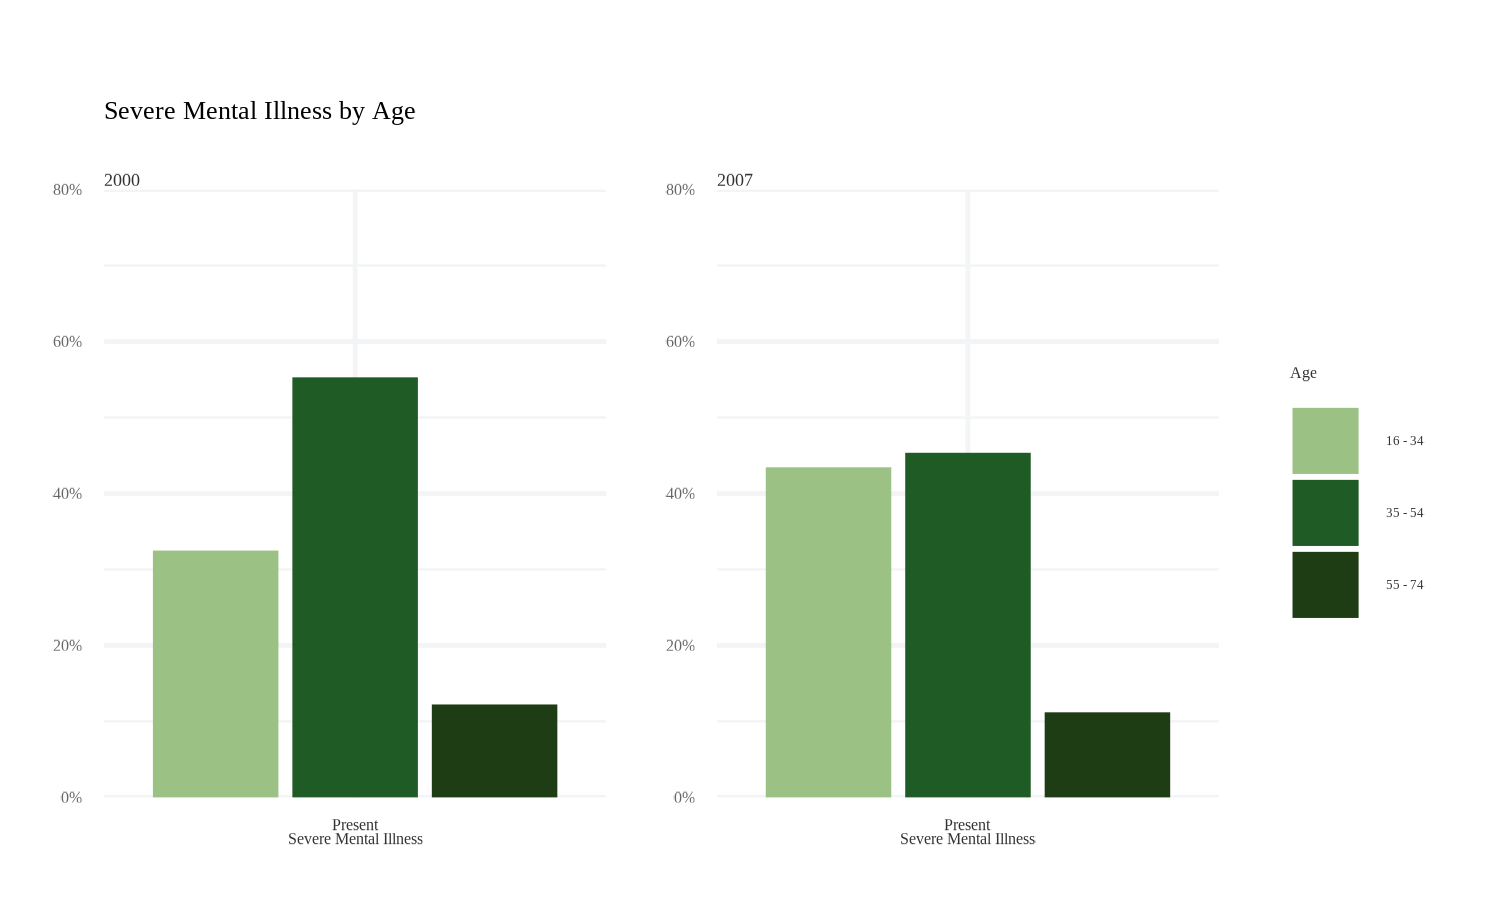
\includegraphics[width=500px,height=300px]{figure/smiage} \caption[Severe Mental Illness' and Age]{Severe Mental Illness' and Age in 2000 and 2007}\label{fig:smiage}
\end{figure}
For the 2000 survey, the rate of individuals indicating they had a severe mental illness in the 16- to 34-year-old age group was 32\% (compared to 35\% with no severe mental illness), in the 35- to 54-year-old age group it was 55\% (compared to 39\% with no severe mental illness), and in the 55- to 74-year-old age group it was 12\% (compared to 26\% with no severe mental illness).

The 2007 survey wave had a similar pattern. The rate of individuals indicating they had a severe mental illness in the 16- to 34-year-old age group was 34\% (compared to 34\% with no severe mental illness), in the 35- to 54-year-old age group it was 45\% (compared to 39\% with no severe mental illness), and in the 55- to 74-year-old age group it was 11\% (compared to 28\% with no severe mental illness).

It is important to note that these statistics reveal a significant disparity in the prevalence of severe mental illness among different age groups, with older adults being less likely to have a severe mental illness. This disparity highlights the need for targeted mental health support and resources for older adults, as they may be less likely to receive the support, they need due to age-related discrimination and biases within the healthcare system. Additionally, the higher rates of severe mental illness among younger adults also highlights the need for mental health support and resources for this age group, as they are more likely to be affected by mental health issues and may face additional barriers to accessing care such as lack of affordable healthcare or difficulty navigating the healthcare system. It is crucial for these disparities to be addressed and ensure that all individuals, regardless of age, have access to the mental health support and resources they need.

However, these should be interpreted with caution because the sample size of those with severe mental illness is relatively small, which could lead to a lack of statistical power and a higher likelihood of sampling error. Additionally, small sample sizes can also lead to a lack of generalizability, meaning that the findings may not be representative of the larger population of individuals with severe mental illness. Therefore, drawing conclusions or making inferences based on such small sample sizes should be done with caution.

Hypothesis testing for the 2000 and 2007 survey wave indicated a statistically significant relationship between age group and severe mental illness presence (Table \ref{tab:results1-charsmi}).

\hypertarget{severe-mental-illness-and-employment-status}{%
\subsection{Severe Mental Illness and Employment Status}\label{severe-mental-illness-and-employment-status}}

In the 2000 survey, 67\% of the overall sample were employed, 2.8\% were unemployed, 0.5\% were unpaid workers, and 30\% were economically inactive. In the 2007 survey, 66\% of the overall sample were employed, 3.2\% were unemployed, 0.3\% were unpaid workers, and 31\% were economically inactive.




\begin{figure}
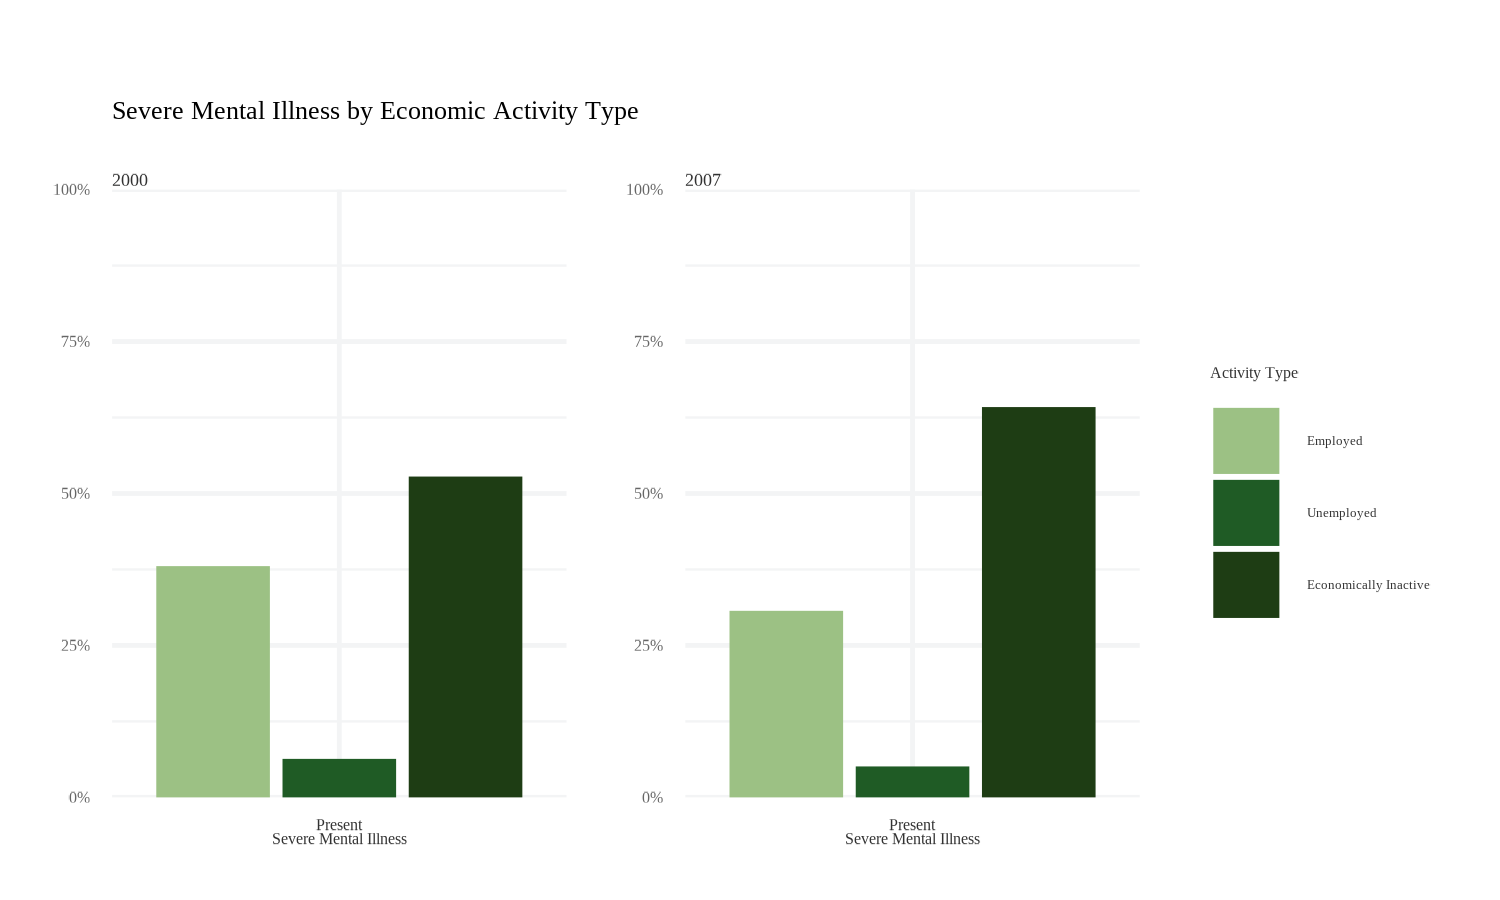
\includegraphics[width=500px,height=300px]{figure/smiat} \caption[Severe Mental Illness and Economic Activity Type]{Severe Mental Illness and Economic Activity Type in 2000 and 2007}\label{fig:smiat}
\end{figure}
In the 2000 survey wave, rates for those employed were 38\% and 62\% (no severe mental illness). The rates for those unemployed were 6.4\% and 2.8\% (no severe mental illness). Unpaid workers had a rate of 2.1\% and 0.5\% (no severe mental illness). For those economically inactive, the rate was 53\% and 29\% (no severe mental illness).

This pattern was similar in the 2007 wave, with rates for those employed at 31\% and 66\% (no severe mental illness). For the unemployed the rate was 5.1\% and 3.2\% (no severe mental illness). The rate for unpaid workers was 0\% and 0.3\% (no severe mental illness). For those economically inactive the rate was 64\% and 36\% (no severe mental illness).

It is important to note that the sample size of individuals with severe mental illness in the survey waves is relatively small, therefore the percentages should be interpreted with caution. Additionally, this data highlights the disparity in employment rates among individuals living with severe mental illness, with a significantly higher percentage of them being economically inactive or unemployed compared to those without severe mental illness. This could be due to a lack of accommodation and support in the workplace for individuals with severe mental illness and highlights the need for more inclusive and supportive policies and practices in the workplace.

\hypertarget{severe-mental-illness-and-employment-status-1}{%
\subsection{Severe Mental Illness and Employment Status}\label{severe-mental-illness-and-employment-status-1}}

For those who were economically active in the 2000 survey wave, the overall rate for those who were full-time employed was 62\%, part-time was 24\%, self-employed was 11\%, and unemployed was 2.8\%. In the 2007 survey wave, the overall rates were 62\% for full-time employed, 24\% for part-time, 11\% for self-employed, and 3.2\% for unemployed.




\begin{figure}
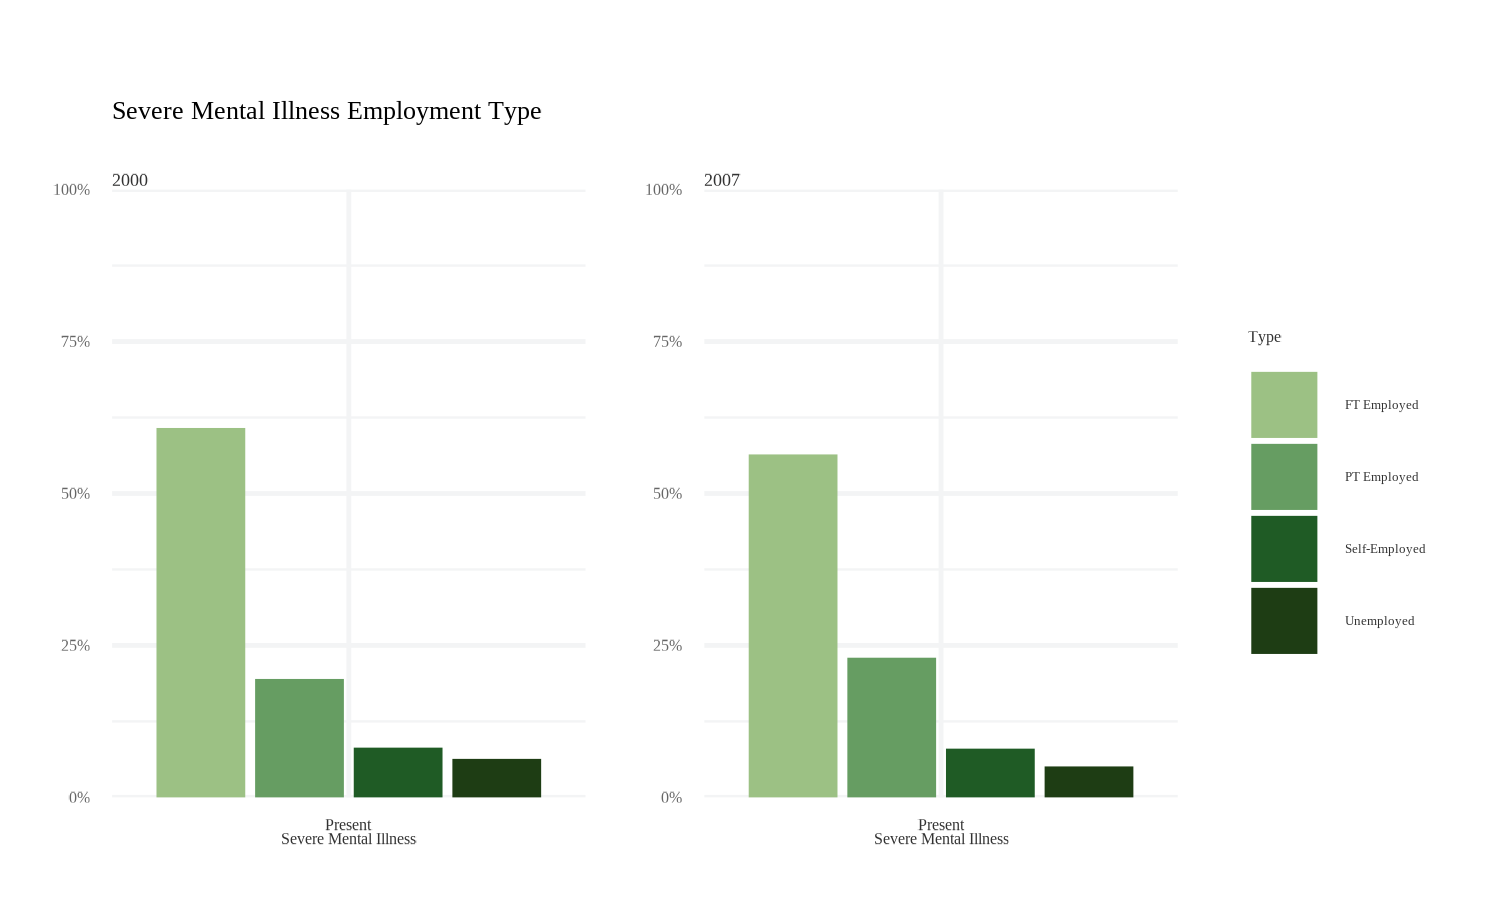
\includegraphics[width=500px,height=300px]{figure/smiet} \caption[Severe Mental Illness and Employment Type]{Severe Mental Illness and Employment Type in 2000 and 2007}\label{fig:smiet}
\end{figure}
In the 2000 survey wave, individuals who were employed full-time and also reported living with a severe mental illness made up 64\% of the full-time employed population (compared to 62\% of those without a severe mental illness). For part-time employees, 21\% reported living with a severe mental illness (compared to 24\% without). For those who were self-employed, 8.6\% reported living with a severe mental illness (compared to 11\% without). For those who were unemployed, 6.7\% reported living with a severe mental illness (compared to 2.7\% without).

Similarly, in the 2007 survey wave, individuals who were employed full-time and also reported living with a severe mental illness made up 61\% of the full-time employed population (compared to 62\% without). For part-time employees, 25\% reported living with a severe mental illness (compared to 24\% without). For those who were self-employed, 8.7\% reported living with a severe mental illness (compared to 11\% without). For those who were unemployed, 5.5\% reported living with a severe mental illness (compared to 3.2\% without).

These numbers highlight the need for better support for individuals with severe mental illness in the workplace, particularly for those who are unemployed and self-employed, as they are more likely to report living with an severe mental illness.

From a social justice lens, these statistics raise important questions about the relationship between employment status and mental health. The high rates of severe mental illness among unemployed individuals in comparison to those who are employed full-time, part-time, and self-employed, suggests that unemployment may be a significant risk factor for severe mental illness. Furthermore, the fact that the rates of severe mental illness are relatively similar across all employment categories raises questions about the systemic issues and barriers that individuals with severe mental illness may face in the workforce.

\hypertarget{type-of-severe-mental-illness-and-economic-activity}{%
\subsection{Type of Severe Mental Illness and Economic Activity}\label{type-of-severe-mental-illness-and-economic-activity}}

The data indicated that individuals who were economically active while living with a severe mental illness were more likely to have a personality disorder, while those who were economically inactive with a severe mental illness were more likely to have a psychosis condition. The overall rates for being economically inactive in 2000 were 30\% and 70\% for being active. In 2007, the overall rates were 31\% for being inactive and 69\% for being active.




\begin{figure}
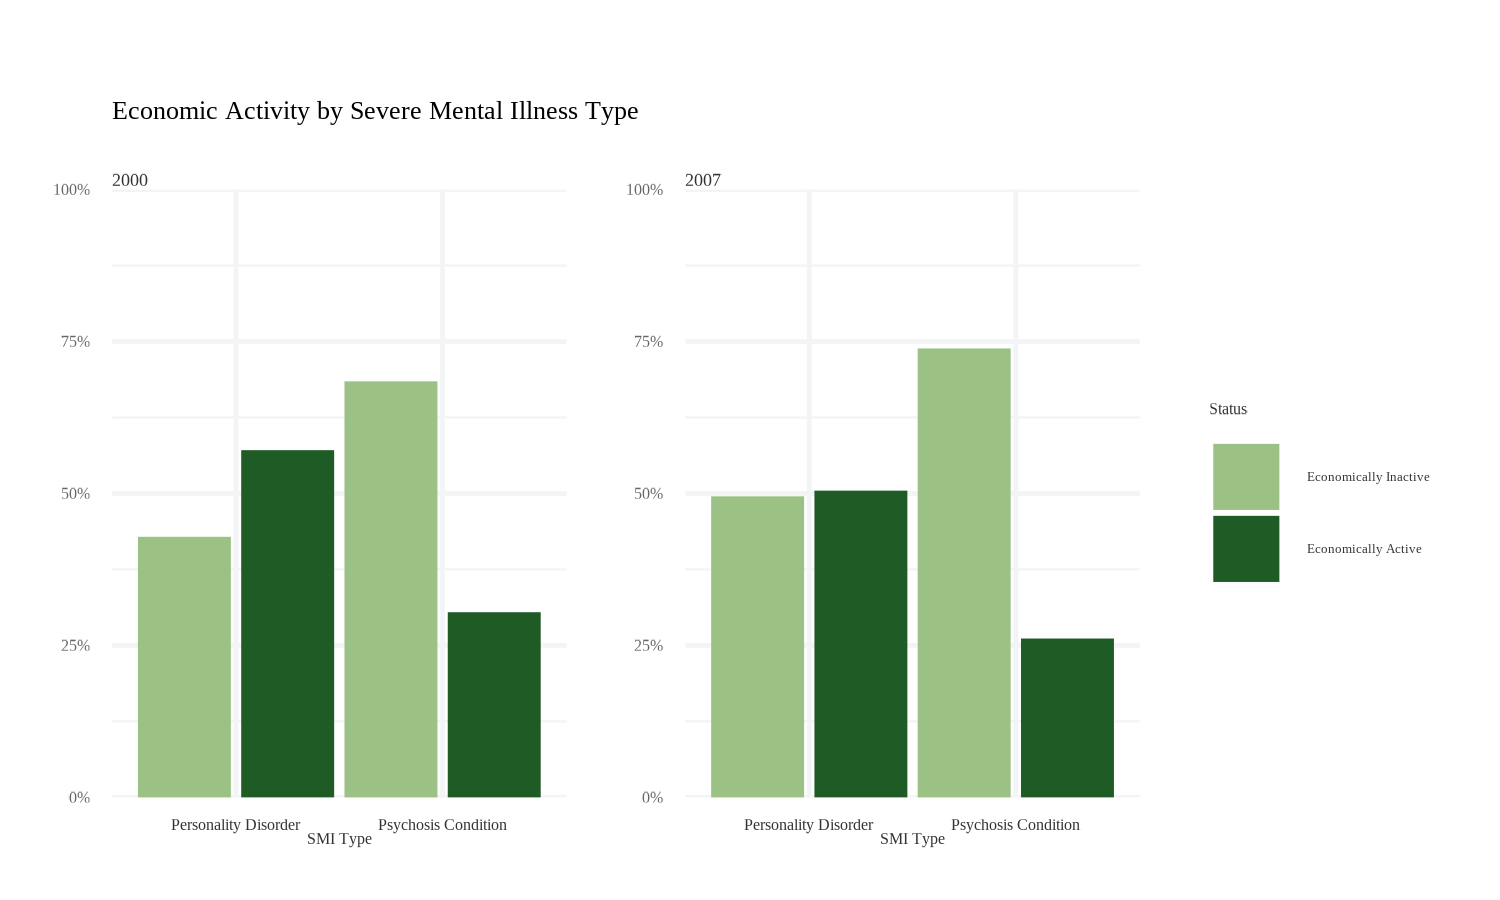
\includegraphics[width=500px,height=300px]{figure/smies} \caption[Employment Status and Severe Mental Illness Type]{Employment Status and Severe Mental Illness Type in 2000 and 2007}\label{fig:smies}
\end{figure}
In 2000, the rate of individuals economically active while living with a severe mental illness condition was 57\% having a personality disorder (43\% having a psychosis condition) and 70\% reporting no severe mental illness. The rate of individuals who are economically inactive with a severe mental illness condition was 43\% having a personality disorder (69\% having a psychosis condition) and 30\% reporting no severe mental illness.

In the 2007 wave, the rate of individuals economically active while living with a severe mental illness condition was 50\% of those individuals reporting living with a personality disorder (26\% as living with a psychosis condition) and 69\% reporting no severe mental illness. The rate of individuals who are economically inactive with an severe mental illness condition is 50\% of individuals living with a personality disorder (74\% of individuals living with a psychosis condition) and 31\% reporting no severe mental illness.

This information highlights the correlation between employment status and the type of severe mental illness an individual may have. It also suggests that individuals who are economically inactive may be more likely to experience psychosis, while those who are economically active may be more likely to experience a personality disorder. This information is important for policymakers and mental health professionals to consider when designing and implementing mental health support and outreach programs.




\begin{figure}
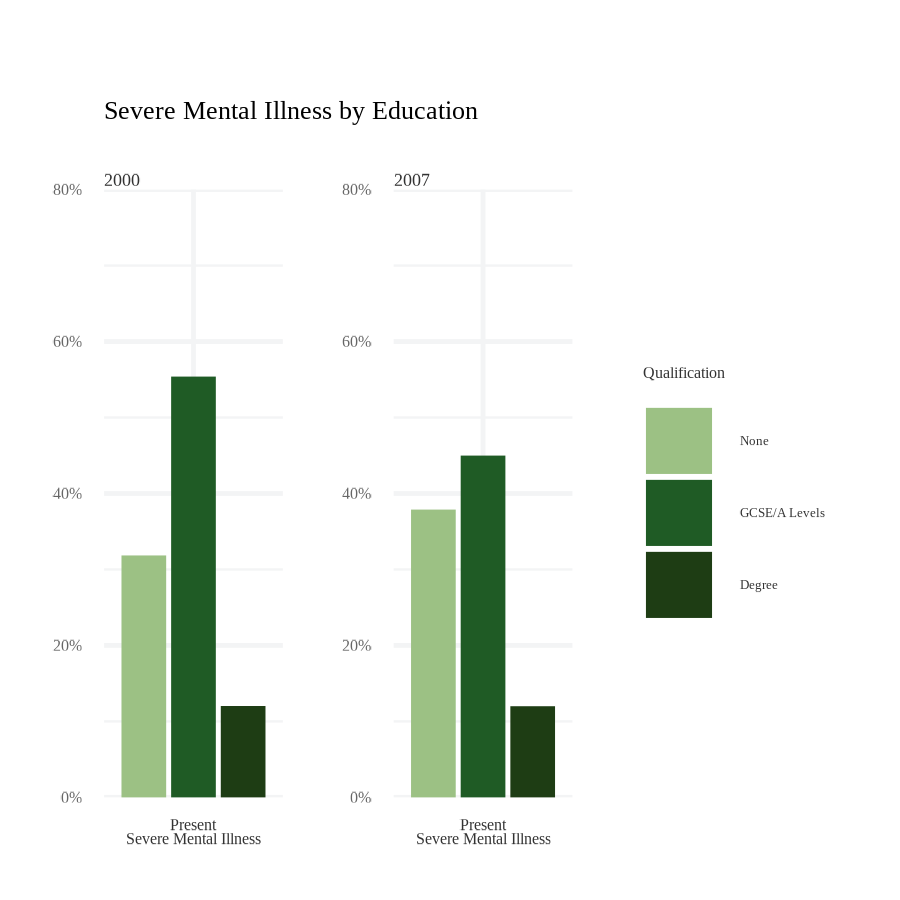
\includegraphics[width=500px,height=300px]{figure/smin} \caption[Employment Status and New Severe Mental Illness]{Employment Status and New Severe Mental Illness in 2000 and 2007}\label{fig:smin}
\end{figure}
In the 2007 survey wave, they introduced new severe mental illness categories, post-traumatic stress disorder (PTSD), and eating disorders. Of those reporting to be economically active, the overall rate for these conditions was 56\%, with 55\% living with PTSD and 57\% living with an eating disorder. Of those individuals who were economically inactive, the overall rate was 44\%, with 45\% reporting PTSD and 43\% reporting having an eating disorder.

It is interesting that the overall rate of individuals reporting to be economically active and living with PTSD or eating disorders was 56\%, with slightly higher rates for PTSD (55\%) and eating disorders (57\%). Additionally, it is also interesting that the overall rate of individuals who were economically inactive and living with PTSD or eating disorders was 44\%, with similar rates for PTSD (45\%) and eating disorders (43\%). This suggests that there may be a correlation between economic activity and the prevalence of PTSD and eating disorders.

\hypertarget{severe-mental-illness-and-reasons-for-economic-inactivity}{%
\subsection{Severe Mental Illness and Reasons for Economic Inactivity}\label{severe-mental-illness-and-reasons-for-economic-inactivity}}

The overall rate of individuals reporting physical health problems as the reason for economic inactivity in the 2000 survey wave was 32\%, and in the 2007 survey wave it was 29\%. For mental health problems, the overall rate was 10\% in 2000 and 9.8\% in 2007. The overall rate for those citing \emph{``no suitable job''} as the reason for economic inactivity was 21\% in 2000 and 22\% in 2007. Lastly, the overall rate of those who reported ``did not want or need a job'' as the reason for economic inactivity was 37\% in 2000 and 39\% in 2007.




\begin{figure}
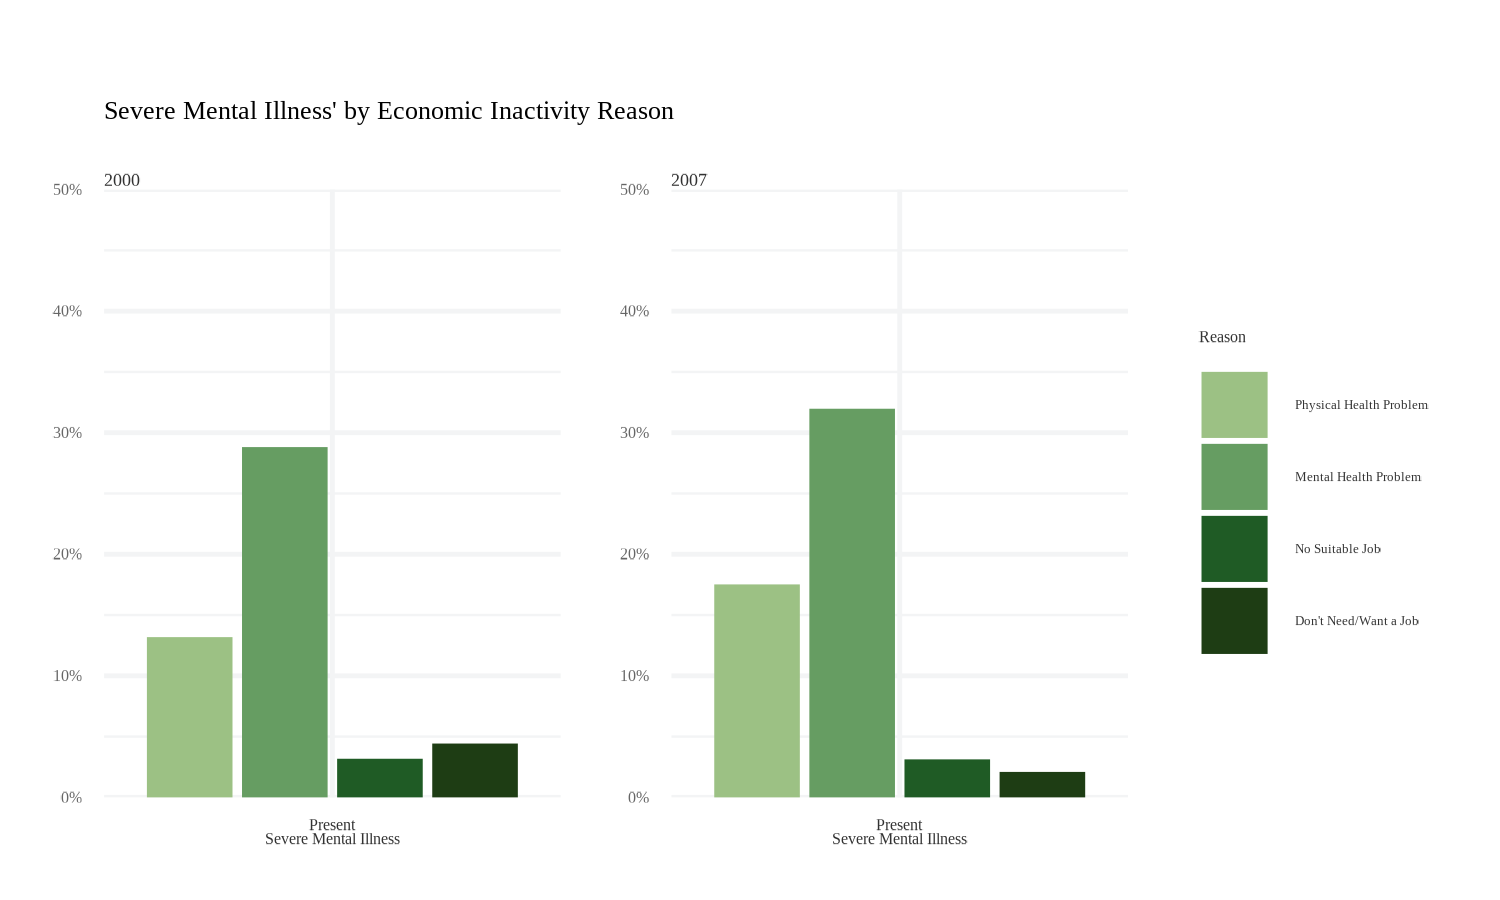
\includegraphics[width=500px,height=300px]{figure/smir} \caption[Severe Mental Illness' and Economic Inactivity Reason]{Severe Mental Illness and Economic Inactivity Reason in 2000 and 2007}\label{fig:smir}
\end{figure}
For those who did indicate they lived with an severe mental illness in the 2000 wave, 27\% (in comparison to 32\% with no severe mental illness) indicated a physical health condition as the reason for their inactivity, 58\% (8.7\% with no severe mental illness) indicated a mental health problem, 6.4\% (21\% without) with severe mental illness indicated that no suitable job was available, and 8.9\% (38\% without severe mental illness) indicated that they did not want or need a job at that time. In 2007 the pattern was similar, with 32\% (29\% without) indicating a physical health condition as the reason for inactivity, 58\% (8.3\% without) indicating a mental health problem, 5.7\% (23\% without) indicated no suitable jobs were available, and 3.8\% (40\% without) indicating that they did not want or need a job at that time.

It seems that individuals who reported living with a severe mental illness in both the 2000 and 2007 survey waves were more likely to report mental health problems as a reason for their economic inactivity compared to those without a severe mental illness. This could indicate a possible lack of support or barriers for individuals with severe mental illness in the workforce. Additionally, the rates of individuals with severe mental illness who reported not wanting or needing a job is relatively low, which may suggest that many of these individuals would prefer to be employed if given the opportunity and support.

\hypertarget{severe-mental-illness-and-education}{%
\subsection{Severe Mental Illness and Education}\label{severe-mental-illness-and-education}}

In the 2000 survey wave, the overall rate of individuals reporting having no qualifications was 27\%, while 51\% reported having GCSE's and A Levels and 22\% reported having a degree. In the 2007 survey wave, the overall rate of individuals reporting to have no qualifications was 23\%, while 47\% reported having GCSE's and A Levels, and 30\% reported having a degree.




\begin{figure}
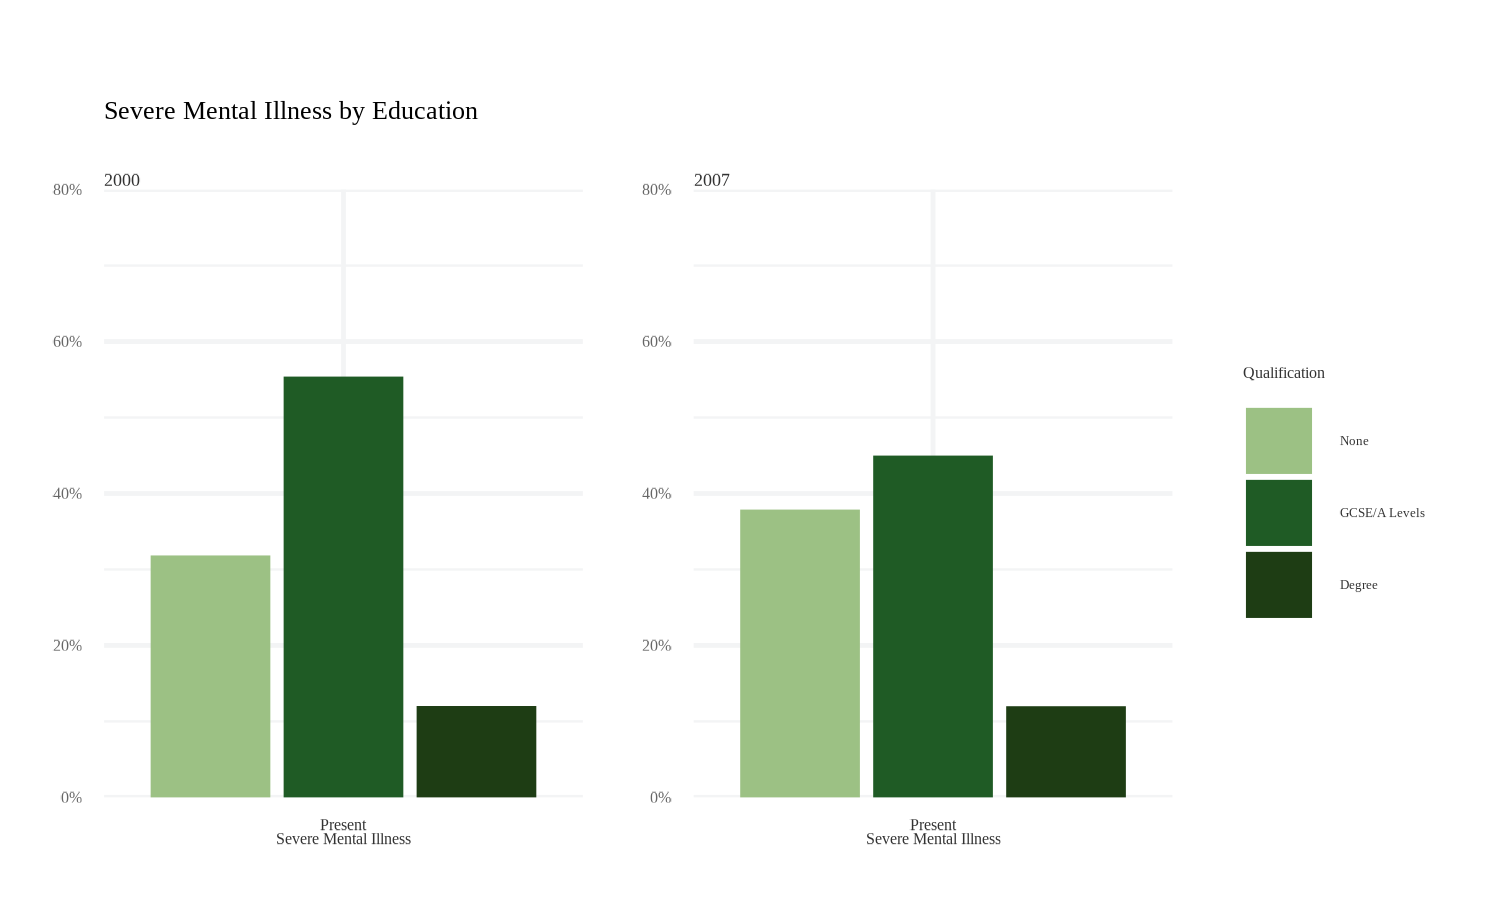
\includegraphics[width=500px,height=300px]{figure/smied} \caption[Severe Mental Illness and Education]{Severe Mental Illness and Education in 2000 and 2007}\label{fig:smied}
\end{figure}
In the 2000 survey wave, 32\% of those living with a severe mental illness had no qualifications (compared to 27\% without a severe mental illness), 56\% had their GCSE or A Levels (compared to 51\% without a severe mental illness), and 12\% had a degree (compared to 22\% without a severe mental illness).

In the 2007 wave, 40\% of those with an severe mental illness had no qualifications (compared to 22\% without an severe mental illness), 47\% had their GCSE's and A Levels (compared to 47\% without an severe mental illness), and 13\% had a degree (compared to 30\% without an severe mental illness).
It is clear that individuals living with an severe mental illness in both survey waves were less likely to have higher levels of education, with a higher proportion having no qualifications or only GCSEs and A Levels compared to those without an severe mental illness. This highlights the need for greater support and resources to be provided to individuals living with an severe mental illness to help them access and complete higher levels of education, as education is often linked to better job opportunities and overall quality of life. From a social justice perspective, it is important to address the systemic barriers that prevent individuals living with an severe mental illness from achieving the same level of educational attainment as those without, and to work towards ensuring that all individuals have equal opportunities to succeed in their education and career goals.

Hypothesis testing found that there was not a statistically significant relationship between having an severe mental illness and educational qualification for the 2000 survey wave, but that there was a significant relationship for those in the 2007 survey wave (Table \ref{tab:results1-charsmi}).

\hypertarget{severe-mental-illness-and-social-class}{%
\subsection{Severe Mental Illness and Social Class}\label{severe-mental-illness-and-social-class}}

The overall rate in the 2000 survey wave was 5.8\% in the unskilled category and 94\% in the skilled category. In the 2007 survey wave the overall rate was 4.6\% in the unskilled category and 95\% in the skilled category.




\begin{figure}
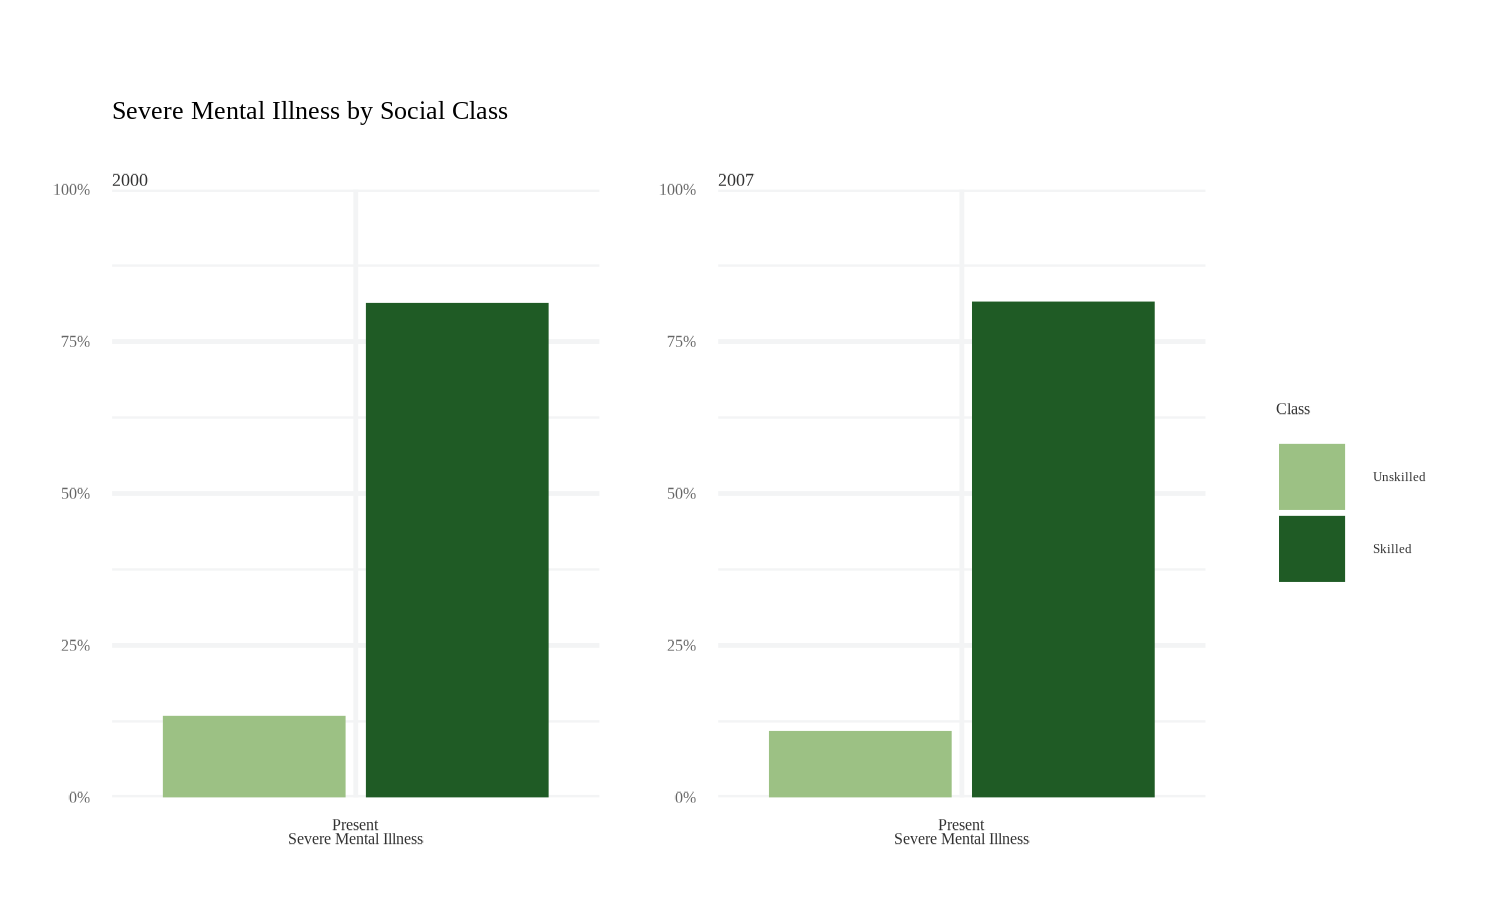
\includegraphics[width=500px,height=300px]{figure/smisc} \caption[Severe Mental Illness and Social Class]{Severe Mental Illness and Social Class in 2000 and 2007}\label{fig:smisc}
\end{figure}
In the 2000 survey wave, 14\% of individuals living with a severe mental illness were classified as unskilled in terms of their social class (compared to 5.7\% of those without a severe mental illness), while 86\% of individuals with a severe mental illness were classified as skilled (compared to 94\% of those without a severe mental illness). In the 2007 survey wave, 12\% of individuals with a severe mental illness were classified as unskilled (compared to 4.5\% of those without a severe mental illness), and 88\% of individuals with an severe mental illness were classified as skilled (compared to 95\% of those without an severe mental illness).

An interesting observation is that individuals living with severe mental illness are underrepresented in the skilled category compared to those without severe mental illness. Additionally, individuals living with severe mental illness are more likely to be in the unskilled social class category compared to those without severe mental illness. This may indicate a disparity in employment opportunities and access to education for individuals living with severe mental illness and highlights the need for policies and programs that address these inequalities.

Hypothesis testing found that there was a significant relationship between the presence of a severe mental illness and social class for those in the 2000 and 2007 survey waves (Table \ref{tab:results1-charsmi}).

\hypertarget{severe-mental-illness-and-ethnicity}{%
\subsection{Severe Mental Illness and Ethnicity}\label{severe-mental-illness-and-ethnicity}}

In the 2000 survey wave, the overall rate for white ethnicity was 93\%, with 7.4\% identifying as belonging to another ethnicity. In contrast, in the 2007 survey wave, the overall rate for white ethnicity was 89\%, while 11\% identified as belonging to another ethnicity.




\begin{figure}
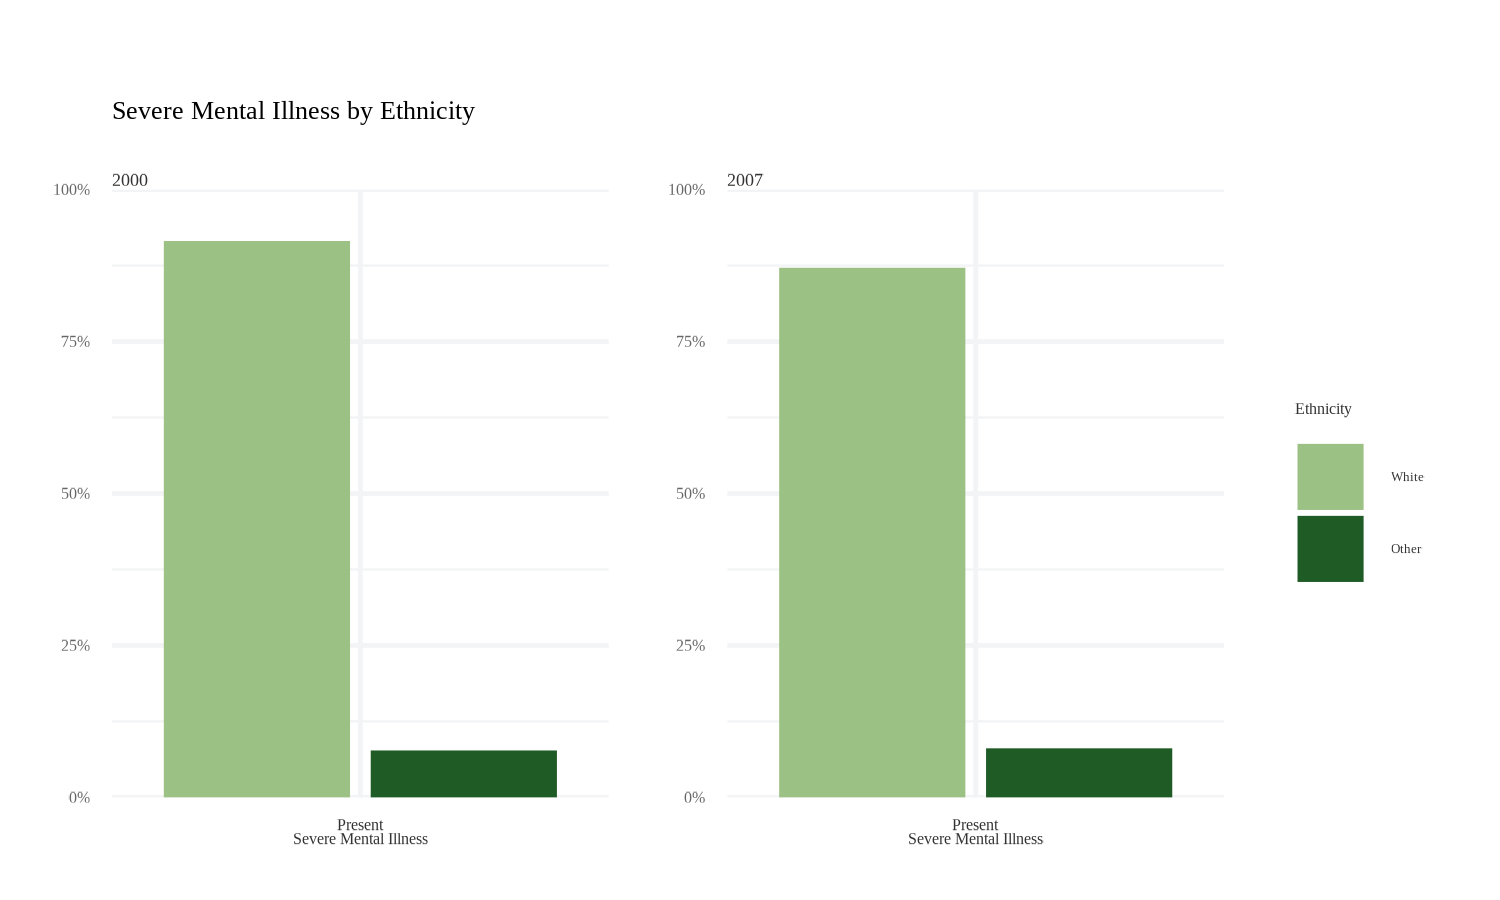
\includegraphics[width=500px,height=300px]{figure/smieth} \caption[Severe Mental Illness and Ethnicity]{Severe Mental Illness and Ethnicity in 2000 and 2007}\label{fig:smieth}
\end{figure}
In the 2000 survey wave, 92\% of individuals with a severe mental illness identified as white, compared to 93\% of those without a severe mental illness. 7.8\% of individuals with a severe mental illness identified as another ethnicity, compared to 7.4\% of those without an severe mental illness. In the 2007 survey wave, 92\% of individuals with an severe mental illness identified as white, compared to 89\% of those without an severe mental illness. 8.5\% of individuals with an severe mental illness identified as another ethnicity, compared to 11\% of those without an severe mental illness.

It is worth noting that the sample size for individuals of another ethnicity was relatively small, so the percentages should be interpreted with caution. Additionally, the fact that a higher proportion of individuals living with severe mental illness belonged to ethnic minorities in comparison to those without severe mental illness may indicate a potential bias in access to mental health services and resources for these individuals. This highlights the need for further research and addressing the disparities in access to mental health services for marginalized communities.

Hypothesis testing did not find a significant relationship between the presence of severe mental illness and ethnicity in the 2000 or 2007 survey waves (Table \ref{tab:results1-charsmi}).

\hypertarget{severe-mental-illness-and-physical-health}{%
\subsection{Severe Mental Illness and Physical Health}\label{severe-mental-illness-and-physical-health}}

The overall rate for the 2000 and 2007 survey waves was 82\% for individuals reporting no physical health condition and 18\% for individuals reporting a physical health condition present. This suggests that the rate of physical health conditions remained consistent over the seven-year period.




\begin{figure}
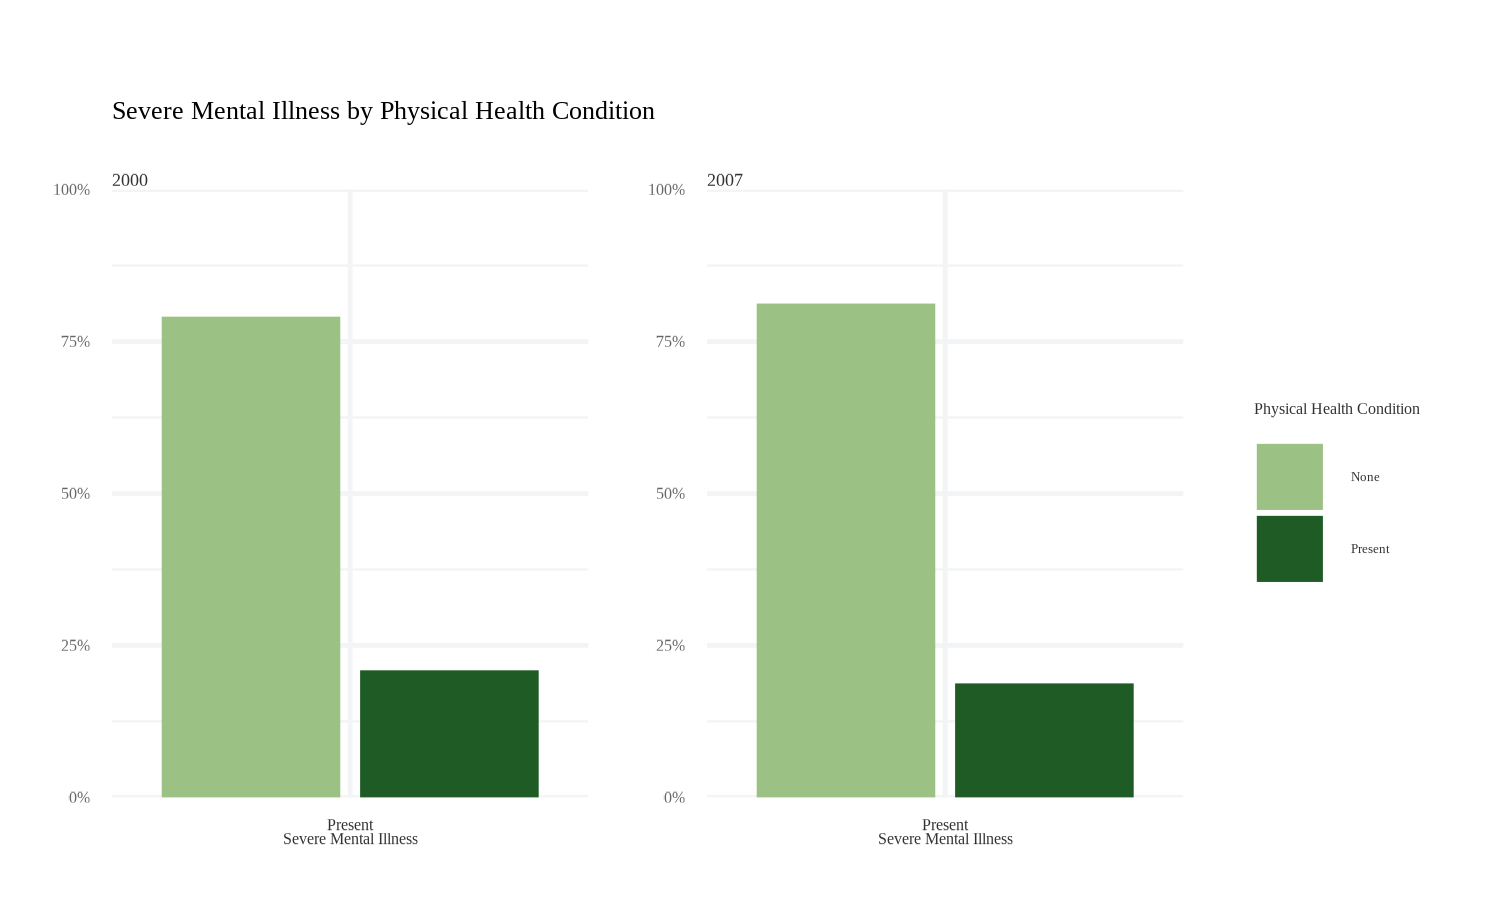
\includegraphics[width=500px,height=300px]{figure/smiphc} \caption[Severe Mental Illness and Physical Health Condition]{Severe Mental Illness and Physical Health Condition in 2000 and 2007}\label{fig:smiphc}
\end{figure}
In the 2000 survey wave, 79\% of individuals living with a severe mental illness reported no physical health condition and 21\% reported living with a physical health condition. In comparison, 82\% of individuals without a severe mental illness reported no physical health condition and 18\% reported living with a physical health condition.

In the 2007 survey wave, 81\% of individuals living with a severe mental illness reported no physical health condition and 19\% reported living with a physical health condition. In comparison, 82\% of individuals without an severe mental illness reported no physical health condition and 18\% reported living with a physical health condition.

It is interesting to observe that in both survey waves, the overall rate for those living with a severe mental illness and a physical health condition is relatively similar to those without an severe mental illness and a physical health condition. This suggests that there may be a strong correlation between severe mental illness and physical health conditions and highlights the importance of addressing both mental and physical health issues in individuals with a severe mental illness. Additionally, it could also indicate that the rate of physical health conditions is not higher among those with severe mental illness which means the healthcare system is not providing enough support for their physical health. This could be a potential area for improvement in terms of providing holistic care for individuals with severe mental illness.

Hypothesis testing also found no significant relationship between presence of an severe mental illness and presence of a physical health condition in both the 2000 and 2007 survey waves.

\hypertarget{severe-mental-illness-and-treatment-use}{%
\subsection{Severe Mental Illness and Treatment Use}\label{severe-mental-illness-and-treatment-use}}

In the 2000 survey, the overall rate of individuals reporting not receiving any form of treatment for their severe mental illness was 93\%, 4.6\% reported only taking medication, 1.2\% reported only receiving counseling, and 1.1\% reported receiving both medication and counseling. In the 2007 survey, a similar pattern was observed with 93\% of individuals reporting not receiving any form of treatment, 4.7\% reporting only taking medication, 1.6\% reporting only receiving counseling, and 1.2\% reporting receiving both medication and counseling.




\begin{figure}
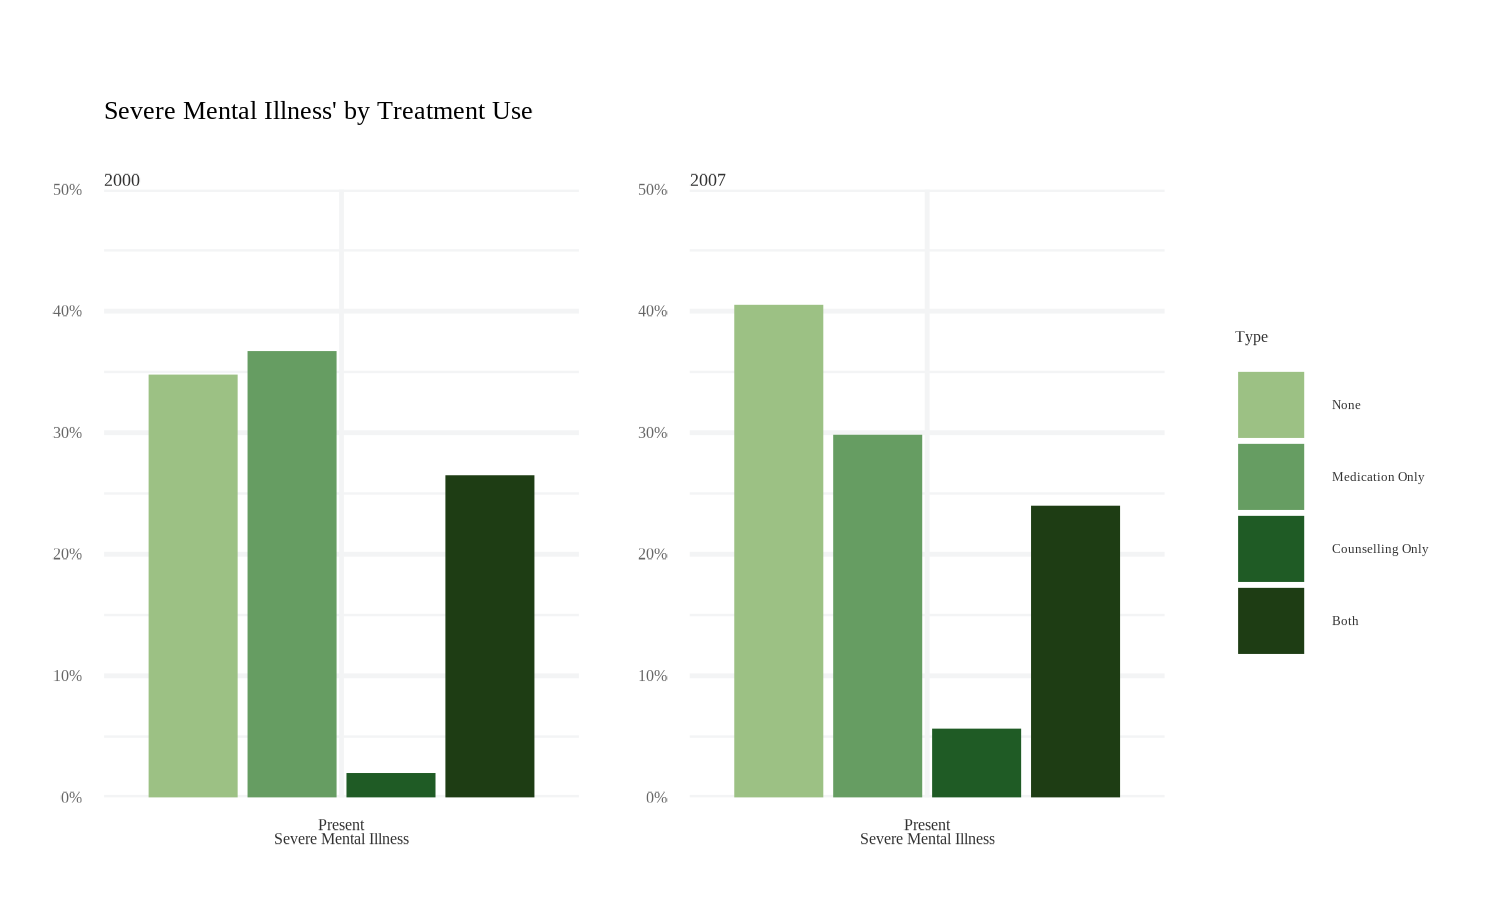
\includegraphics[width=500px,height=300px]{figure/smitrt} \caption[Severe Mental Illness and Treatment Use]{Severe Mental Illness and Treatment Use in 2000 and 2007}\label{fig:smitrt}
\end{figure}
In the 2000 survey wave, 35\% of individuals who did not take part in any form of mental health treatment also reported living with a severe mental illness, while 94\% reported no severe mental illness present. 37\% of individuals who took medication only as a form of treatment also reported living with a severe mental illness, while 4.4\% reported no severe mental illness. 2.6\% of individuals who took part in both medication and counseling or therapy in combination as a mental health treatment also reported living with a severe mental illness, while 0.9\% reported no severe mental illness presence. 1.2\% of individuals who took part in counseling or therapy on their own as a form of mental health treatment also reported living with a severe mental illness, while 1.2\% reported no severe mental illness present.

In the 2007 survey wave, 41\% of individuals who did not take part in any form of mental health treatment also reported living with a severe mental illness, while 93\% reported no severe mental illness present. 30\% of individuals who took medication only as a form of treatment also reported living with a severe mental illness, while 4.5\% reported no severe mental illness. 24\% of individuals who took part in both medication and counseling or therapy in combination as a mental health treatment also reported living with an severe mental illness, while 1\% reported no severe mental illness presence. 5.7\% of individuals who took part in counseling or therapy on their own as a form of mental health treatment also reported living with a severe mental illness, while 1.5\% reported no severe mental illness present.

Hypothesis testing also found a significant relationship between presence of an severe mental illness and having mental health treatment in both the 2000 and 2007 survey waves (Table \ref{tab:results1-charsmi}).

\hypertarget{severe-mental-illness-and-mental-health-service-use}{%
\subsection{Severe Mental Illness and Mental Health Service Use}\label{severe-mental-illness-and-mental-health-service-use}}

Engaging with mental health services was derived from individuals reporting that they had received health care for a mental health condition, including their GP, inpatient and outpatient hospital appointments and community mental health teams. The overall rate in 2000 for not having used any services was 88\% and 12\% for having used services. In 2007 the overall rate was the same.




\begin{figure}
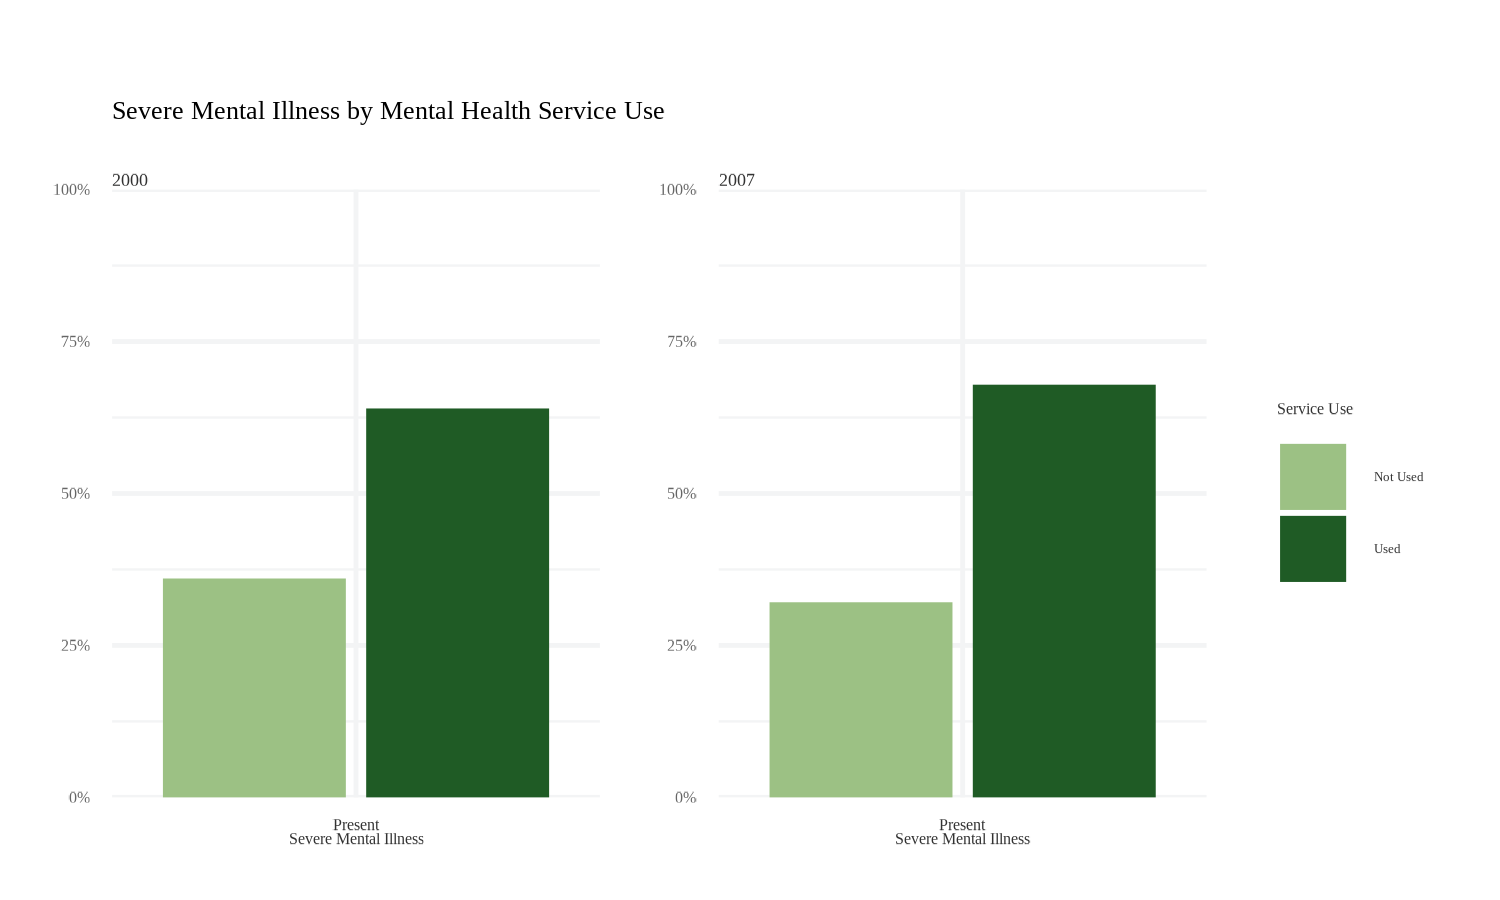
\includegraphics[width=500px,height=300px]{figure/smisu} \caption[Severe Mental Illness and Mental Health Service Use]{Severe Mental Illness and Mental Health Service Use in 2000 and 2007}\label{fig:smisu}
\end{figure}
In the 2000 survey wave, 36\% of individuals who had not used any mental health services reported living with a severe mental illness, compared to 89\% who reported not having a severe mental illness. Among those who reported using mental health services, 64\% reported living with a severe mental illness and 11\% reported not having a severe mental illness.

Similarly, in the 2007 survey wave, 32\% of individuals who had not used any mental health services reported living with an severe mental illness, compared to 89\% who reported not having an severe mental illness. Among those who reported using mental health services, 68\% reported living with an severe mental illness and 11\% reported not having an severe mental illness.

From a social justice lens, it is interesting to note that in the 2000 and 2007 survey waves, a higher proportion of individuals who reported using mental health services also reported living with a severe mental illness compared to those who did not report using mental health services. This suggests that individuals living with severe mental illness may be more likely to seek out and utilize mental health services and highlights the importance of ensuring that these services are accessible and effective for this population. Additionally, it's worth noting that the rate of those who did not report living with an severe mental illness was quite similar between the two groups, which suggests that the lack of use of mental health services is not only related to the presence or absence of severe mental illness but also other factors like stigma, lack of access, or unawareness of services.

Hypothesis testing found a significant relationship between using any mental health service and an severe mental illness being present in both the 2000 and 2007 survey waves (\ref{tab:results1-charsmi}).

\hypertarget{summary-2}{%
\section{Summary}\label{summary-2}}

In Chapter @(chapter5), the survey data from 2000 and 2007 waves were analyzed to examine the relationship between severe mental illness and employment status. The results showed that individuals living with a severe mental illness were more likely to be unemployed or economically inactive compared to those without a severe mental illness. Additionally, individuals with an severe mental illness were more likely to have a personality disorder if they were economically active and more likely to have a psychosis condition if they were economically inactive.

In terms of education and social class, the data revealed that individuals with a severe mental illness were less likely to have higher levels of education and were more likely to be in the unskilled social class category. Furthermore, the data revealed a higher rate of individuals with an severe mental illness identifying as white and a lower rate identifying with another ethnicity.

The data also showed that in both 2000 and 2007, a majority of individuals with an severe mental illness did not receive any form of treatment for their condition. Those who did receive treatment were more likely to have a combination of medication and counselling or therapy, with a smaller percentage receiving only medication or counselling.

Overall, the data from Chapter \ref{chapter5} highlights the significant disparities in employment status, education, social class, and treatment access for individuals living with a severe mental illness. These findings suggest that individuals with an severe mental illness face significant barriers to social and economic opportunities and highlight the need for targeted interventions to address these disparities.

The research questions are further explored in Chapter \ref{chapter6}.

\hypertarget{chapter6}{%
\chapter{Results 2: Models}\label{chapter6}}

\hypertarget{chapter-overview-5}{%
\section{Chapter Overview}\label{chapter-overview-5}}

This chapter reports results of the analyses conducted to answer the research questions:
\begin{enumerate}
\def\labelenumi{\arabic{enumi}.}
\tightlist
\item
  How has the impact of common mental health disorders and severe mental illness on employment status changed since 2000 in England?
\item
  How do employment status patterns for individuals with common mental health disorders and severe mental illness compared to the rest of the population in England in 2007?
\item
  Is the relationship of severe mental illness to employment status different from the relationship of common mental health disorders to employment status in England?
\item
  How does living with common mental health disorders and severe mental illness affect the entrance of young adults (16-35 years old) to the labour force, in comparison to young adults without common mental health disorders and severe mental illness?
\item
  Are the effects of common mental health disorders and severe mental illness on employment status mitigated or exacerbated by other barriers or enablers, such as socioeconomic status, ethnicity, education, physical health, involvement in services?
\end{enumerate}
The first sections of this chapter cover economic activity and employment status, the third section relates to common mental health disorders and the fourth to severe mental illness. As discussed in the previous chapter, both survey waves were also made comparable to each other. This chapter explores employment outcomes in relation to common mental health disorders and severe mental illness, and then examines the variations by common mental health disorder and severe mental illness type. Nested models were used, by first looking at the factors associated with being economically active rather than inactive; and then for those who were economically active, distinguishing those in employment from those who were unemployed.

A brief summary of the results is also provided. Discussion of the key findings and implications are found in Chapter \ref{chapter7}.

\hypertarget{economic-activity-1}{%
\section{Economic Activity}\label{economic-activity-1}}

This section covers results of logistic regression models applied to economic activity. In total, two models are reported - one for each survey year. The dependent variable was economic activity, with the default category being economically inactive. The independent variables for the models were gender (male and female), age (16 -- 34, 35 -- 54, 55 -- 74), ethnicity (white and other), social class (unskilled and skilled), education (none, GCSE/A Level, and degree), physical health (present or not), common mental health disorder (present or not), and severe mental illness (present or not). Descriptive for these can be seen in Chapter \ref{chapter5}.

\hypertarget{model-results-for-economic-activity}{%
\subsection{Model Results for Economic Activity}\label{model-results-for-economic-activity}}

There were 6,920 individuals included in the model for the year 2000 and 5,750 individuals in the year 2007 for economic activity (Table \ref{tab:results2-econmod}) shows model output, including adjusted odds ratios). Adjusted odds ratios for gender showed that females were less likely to be economically active than males and this difference was also statistically significant. The adjusted odds ratios for gender revealed that females were less likely to be economically active than males, and this difference was statistically significant. This disparity is particularly striking, as it indicates that women are more likely than men to be out of the labour force. This gender difference is greater than that between those with chronic mental health conditions and those without, highlighting the significant impact of societal expectations and gender roles on women's participation in the labour force.

This disparity in economic activity is likely linked to traditional gender roles and societal expectations, which often place a higher value on women's caregiving responsibilities over paid employment. As such, many women may prioritize, or be conditioned to prioritize, caregiving responsibilities over paid work, which can lead to them being out of the labour force. Additionally, it may also reflect the fact that women tend to retire earlier than men, which can also contribute to the difference in economic activity.

It is important to note that this disparity in economic activity has far-reaching consequences, as it can lead to a lack of economic security and financial independence for women. It's worth highlighting this disparity as it calls for society to challenge traditional gender roles and societal expectations, and to create policies and opportunities that support women's participation in the labour force and promote gender equality.

Ratios for age groups decreased from younger to older, with those in the 55- to 74-year-old age band the least likely to be economically active in comparison to the reference group (the 16- to 34-year-old age band) and this was also statistically significant. The 35- to 54-year-old age group, however, was not significantly different from the default (16-34). Other groups that showed reduced odds of economic activity in comparison to their reference category were the presence of a physical health condition. These were all also statistically significant.

Ethnicity (indicated as ``other'') also showed reduced odds of being economically active in comparison to the reference group of being white but was not statistically significant. However, social class and educational qualifications did show increased odds of being economically active in those individuals who were skilled (in comparison to the reference group of unskilled) in one year, but lower in the next, and in those who had gained their GCSE's or A Levels or degree (in comparison to having no qualifications at all). Social class was not found to be statistically significant, whereas educational qualifications were statistically significant.

In terms of the main focus for this analysis, the Table shows that the presence of a common mental health disorder and of a severe mental illness both reduced the likelihood of being economically active. Table \ref{tab:results2-econmod} shows that those with common mental health disorders are less likely to be economically active than those with severe mental illness, although the sample size for those with a severe mental illness present across both survey waves is small (56 and 46 people) in comparison to those with common mental health disorders present (1,199 and 1,088, see Chapter \ref{chapter5} for descriptive statistics).

\providecommand{\huxb}[2]{\arrayrulecolor[RGB]{#1}\global\arrayrulewidth=#2pt}
  \providecommand{\huxvb}[2]{\color[RGB]{#1}\vrule width #2pt}
  \providecommand{\huxtpad}[1]{\rule{0pt}{#1}}
  \providecommand{\huxbpad}[1]{\rule[-#1]{0pt}{#1}}
\begin{table}[ht]
\begin{centerbox}
\begin{threeparttable}
 \setlength{\tabcolsep}{0pt}
\begin{adjustbox}{width=1\textwidth}
\normalsize
\begin{tabular}{l l l l l l l l l}


\hhline{>{\arrayrulecolor[RGB]{0, 0, 0}\global\arrayrulewidth=0.4pt}->{\arrayrulecolor[RGB]{0, 0, 0}\global\arrayrulewidth=0.4pt}->{\arrayrulecolor[RGB]{0, 0, 0}\global\arrayrulewidth=0.4pt}->{\arrayrulecolor[RGB]{0, 0, 0}\global\arrayrulewidth=0.4pt}->{\arrayrulecolor[RGB]{0, 0, 0}\global\arrayrulewidth=0.4pt}->{\arrayrulecolor[RGB]{0, 0, 0}\global\arrayrulewidth=0.4pt}->{\arrayrulecolor[RGB]{0, 0, 0}\global\arrayrulewidth=0.4pt}->{\arrayrulecolor[RGB]{0, 0, 0}\global\arrayrulewidth=0.4pt}->{\arrayrulecolor[RGB]{0, 0, 0}\global\arrayrulewidth=0.4pt}-}
\arrayrulecolor{black}

\multicolumn{1}{!{\color[RGB]{0, 0, 0}\vrule width 0pt}l!{\color[RGB]{0, 0, 0}\vrule width 0pt}}{\rule{0pt}{1pt + 1em}\raggedright \hspace{0pt} \textbf{{\fontsize{14pt}{16.8pt}\selectfont 
}} \hspace{1pt}\rule[-1pt]{0pt}{1pt}} &
\multicolumn{4}{c!{\color[RGB]{0, 0, 0}\vrule width 0pt}}{\rule{0pt}{1pt + 1em}\centering \hspace{1pt} \textbf{{\fontsize{14pt}{16.8pt}\selectfont \textbf{2000 Wave}
}} \hspace{1pt}\rule[-1pt]{0pt}{1pt}} &
\multicolumn{4}{c!{\color[RGB]{0, 0, 0}\vrule width 0pt}}{\rule{0pt}{1pt + 1em}\centering \hspace{1pt} \textbf{{\fontsize{14pt}{16.8pt}\selectfont \textbf{2007 Wave}
}} \hspace{1pt}\rule[-1pt]{0pt}{1pt}} \tabularnewline[-0.5pt]


\hhline{}
\arrayrulecolor{black}

\multicolumn{1}{!{\color[RGB]{0, 0, 0}\vrule width 0pt}l!{\color[RGB]{0, 0, 0}\vrule width 0pt}}{\rule{0pt}{1pt + 1em}\raggedright \hspace{0pt} \textbf{{\fontsize{14pt}{16.8pt}\selectfont \textbf{Characteristic}
}} \hspace{1pt}\rule[-1pt]{0pt}{1pt}} &
\multicolumn{1}{c!{\color[RGB]{0, 0, 0}\vrule width 0pt}}{\rule{0pt}{1pt + 1em}\centering \hspace{1pt} \textbf{{\fontsize{14pt}{16.8pt}\selectfont \textbf{N}
}} \hspace{1pt}\rule[-1pt]{0pt}{1pt}} &
\multicolumn{1}{c!{\color[RGB]{0, 0, 0}\vrule width 0pt}}{\rule{0pt}{1pt + 1em}\centering \hspace{1pt} \textbf{{\fontsize{14pt}{16.8pt}\selectfont \textbf{OR}
}} \hspace{1pt}\rule[-1pt]{0pt}{1pt}} &
\multicolumn{1}{c!{\color[RGB]{0, 0, 0}\vrule width 0pt}}{\rule{0pt}{1pt + 1em}\centering \hspace{1pt} \textbf{{\fontsize{14pt}{16.8pt}\selectfont \textbf{95\% CI}
}} \hspace{1pt}\rule[-1pt]{0pt}{1pt}} &
\multicolumn{1}{c!{\color[RGB]{0, 0, 0}\vrule width 0pt}}{\rule{0pt}{1pt + 1em}\centering \hspace{1pt} \textbf{{\fontsize{14pt}{16.8pt}\selectfont \textbf{p-value}
}} \hspace{1pt}\rule[-1pt]{0pt}{1pt}} &
\multicolumn{1}{c!{\color[RGB]{0, 0, 0}\vrule width 0pt}}{\rule{0pt}{1pt + 1em}\centering \hspace{1pt} \textbf{{\fontsize{14pt}{16.8pt}\selectfont \textbf{N}
}} \hspace{1pt}\rule[-1pt]{0pt}{1pt}} &
\multicolumn{1}{c!{\color[RGB]{0, 0, 0}\vrule width 0pt}}{\rule{0pt}{1pt + 1em}\centering \hspace{1pt} \textbf{{\fontsize{14pt}{16.8pt}\selectfont \textbf{OR}
}} \hspace{1pt}\rule[-1pt]{0pt}{1pt}} &
\multicolumn{1}{c!{\color[RGB]{0, 0, 0}\vrule width 0pt}}{\rule{0pt}{1pt + 1em}\centering \hspace{1pt} \textbf{{\fontsize{14pt}{16.8pt}\selectfont \textbf{95\% CI}
}} \hspace{1pt}\rule[-1pt]{0pt}{1pt}} &
\multicolumn{1}{c!{\color[RGB]{0, 0, 0}\vrule width 0pt}}{\rule{0pt}{1pt + 1em}\centering \hspace{1pt} \textbf{{\fontsize{14pt}{16.8pt}\selectfont \textbf{p-value}
}} \hspace{0pt}\rule[-1pt]{0pt}{1pt}} \tabularnewline[-0.5pt]


\hhline{>{\arrayrulecolor[RGB]{0, 0, 0}\global\arrayrulewidth=0.4pt}->{\arrayrulecolor[RGB]{0, 0, 0}\global\arrayrulewidth=0.4pt}->{\arrayrulecolor[RGB]{0, 0, 0}\global\arrayrulewidth=0.4pt}->{\arrayrulecolor[RGB]{0, 0, 0}\global\arrayrulewidth=0.4pt}->{\arrayrulecolor[RGB]{0, 0, 0}\global\arrayrulewidth=0.4pt}->{\arrayrulecolor[RGB]{0, 0, 0}\global\arrayrulewidth=0.4pt}->{\arrayrulecolor[RGB]{0, 0, 0}\global\arrayrulewidth=0.4pt}->{\arrayrulecolor[RGB]{0, 0, 0}\global\arrayrulewidth=0.4pt}->{\arrayrulecolor[RGB]{0, 0, 0}\global\arrayrulewidth=0.4pt}-}
\arrayrulecolor{black}

\multicolumn{1}{!{\color[RGB]{0, 0, 0}\vrule width 0pt}l!{\color[RGB]{0, 0, 0}\vrule width 0pt}}{\rule{0pt}{1pt + 1em}\raggedright \hspace{0pt} \textbf{{\fontsize{14pt}{16.8pt}\selectfont Gender}} \hspace{1pt}\rule[-1pt]{0pt}{1pt}} &
\multicolumn{1}{c!{\color[RGB]{0, 0, 0}\vrule width 0pt}}{\rule{0pt}{1pt + 1em}\centering \hspace{1pt} {\fontsize{14pt}{16.8pt}\selectfont 6,920} \hspace{1pt}\rule[-1pt]{0pt}{1pt}} &
\multicolumn{1}{c!{\color[RGB]{0, 0, 0}\vrule width 0pt}}{\rule{0pt}{1pt + 1em}\centering \hspace{1pt} {\fontsize{14pt}{16.8pt}\selectfont } \hspace{1pt}\rule[-1pt]{0pt}{1pt}} &
\multicolumn{1}{c!{\color[RGB]{0, 0, 0}\vrule width 0pt}}{\rule{0pt}{1pt + 1em}\centering \hspace{1pt} {\fontsize{14pt}{16.8pt}\selectfont } \hspace{1pt}\rule[-1pt]{0pt}{1pt}} &
\multicolumn{1}{c!{\color[RGB]{0, 0, 0}\vrule width 0pt}}{\rule{0pt}{1pt + 1em}\centering \hspace{1pt} {\fontsize{14pt}{16.8pt}\selectfont } \hspace{1pt}\rule[-1pt]{0pt}{1pt}} &
\multicolumn{1}{c!{\color[RGB]{0, 0, 0}\vrule width 0pt}}{\rule{0pt}{1pt + 1em}\centering \hspace{1pt} {\fontsize{14pt}{16.8pt}\selectfont 5,750} \hspace{1pt}\rule[-1pt]{0pt}{1pt}} &
\multicolumn{1}{c!{\color[RGB]{0, 0, 0}\vrule width 0pt}}{\rule{0pt}{1pt + 1em}\centering \hspace{1pt} {\fontsize{14pt}{16.8pt}\selectfont } \hspace{1pt}\rule[-1pt]{0pt}{1pt}} &
\multicolumn{1}{c!{\color[RGB]{0, 0, 0}\vrule width 0pt}}{\rule{0pt}{1pt + 1em}\centering \hspace{1pt} {\fontsize{14pt}{16.8pt}\selectfont } \hspace{1pt}\rule[-1pt]{0pt}{1pt}} &
\multicolumn{1}{c!{\color[RGB]{0, 0, 0}\vrule width 0pt}}{\rule{0pt}{1pt + 1em}\centering \hspace{1pt} {\fontsize{14pt}{16.8pt}\selectfont } \hspace{0pt}\rule[-1pt]{0pt}{1pt}} \tabularnewline[-0.5pt]


\hhline{}
\arrayrulecolor{black}

\multicolumn{1}{!{\color[RGB]{0, 0, 0}\vrule width 0pt}l!{\color[RGB]{0, 0, 0}\vrule width 0pt}}{\rule{0pt}{1pt + 1em}\raggedright \hspace{0pt} {\fontsize{14pt}{16.8pt}\selectfont Male} \hspace{1pt}\rule[-1pt]{0pt}{1pt}} &
\multicolumn{1}{c!{\color[RGB]{0, 0, 0}\vrule width 0pt}}{\rule{0pt}{1pt + 1em}\centering \hspace{1pt} {\fontsize{14pt}{16.8pt}\selectfont } \hspace{1pt}\rule[-1pt]{0pt}{1pt}} &
\multicolumn{1}{c!{\color[RGB]{0, 0, 0}\vrule width 0pt}}{\rule{0pt}{1pt + 1em}\centering \hspace{1pt} {\fontsize{14pt}{16.8pt}\selectfont —} \hspace{1pt}\rule[-1pt]{0pt}{1pt}} &
\multicolumn{1}{c!{\color[RGB]{0, 0, 0}\vrule width 0pt}}{\rule{0pt}{1pt + 1em}\centering \hspace{1pt} {\fontsize{14pt}{16.8pt}\selectfont —} \hspace{1pt}\rule[-1pt]{0pt}{1pt}} &
\multicolumn{1}{c!{\color[RGB]{0, 0, 0}\vrule width 0pt}}{\rule{0pt}{1pt + 1em}\centering \hspace{1pt} {\fontsize{14pt}{16.8pt}\selectfont } \hspace{1pt}\rule[-1pt]{0pt}{1pt}} &
\multicolumn{1}{c!{\color[RGB]{0, 0, 0}\vrule width 0pt}}{\rule{0pt}{1pt + 1em}\centering \hspace{1pt} {\fontsize{14pt}{16.8pt}\selectfont } \hspace{1pt}\rule[-1pt]{0pt}{1pt}} &
\multicolumn{1}{c!{\color[RGB]{0, 0, 0}\vrule width 0pt}}{\rule{0pt}{1pt + 1em}\centering \hspace{1pt} {\fontsize{14pt}{16.8pt}\selectfont —} \hspace{1pt}\rule[-1pt]{0pt}{1pt}} &
\multicolumn{1}{c!{\color[RGB]{0, 0, 0}\vrule width 0pt}}{\rule{0pt}{1pt + 1em}\centering \hspace{1pt} {\fontsize{14pt}{16.8pt}\selectfont —} \hspace{1pt}\rule[-1pt]{0pt}{1pt}} &
\multicolumn{1}{c!{\color[RGB]{0, 0, 0}\vrule width 0pt}}{\rule{0pt}{1pt + 1em}\centering \hspace{1pt} {\fontsize{14pt}{16.8pt}\selectfont } \hspace{0pt}\rule[-1pt]{0pt}{1pt}} \tabularnewline[-0.5pt]


\hhline{}
\arrayrulecolor{black}

\multicolumn{1}{!{\color[RGB]{0, 0, 0}\vrule width 0pt}l!{\color[RGB]{0, 0, 0}\vrule width 0pt}}{\rule{0pt}{1pt + 1em}\raggedright \hspace{0pt} {\fontsize{14pt}{16.8pt}\selectfont Female} \hspace{1pt}\rule[-1pt]{0pt}{1pt}} &
\multicolumn{1}{c!{\color[RGB]{0, 0, 0}\vrule width 0pt}}{\rule{0pt}{1pt + 1em}\centering \hspace{1pt} {\fontsize{14pt}{16.8pt}\selectfont } \hspace{1pt}\rule[-1pt]{0pt}{1pt}} &
\multicolumn{1}{c!{\color[RGB]{0, 0, 0}\vrule width 0pt}}{\rule{0pt}{1pt + 1em}\centering \hspace{1pt} {\fontsize{14pt}{16.8pt}\selectfont 0.39} \hspace{1pt}\rule[-1pt]{0pt}{1pt}} &
\multicolumn{1}{c!{\color[RGB]{0, 0, 0}\vrule width 0pt}}{\rule{0pt}{1pt + 1em}\centering \hspace{1pt} {\fontsize{14pt}{16.8pt}\selectfont 0.34, 0.45} \hspace{1pt}\rule[-1pt]{0pt}{1pt}} &
\multicolumn{1}{c!{\color[RGB]{0, 0, 0}\vrule width 0pt}}{\rule{0pt}{1pt + 1em}\centering \hspace{1pt} \textbf{{\fontsize{14pt}{16.8pt}\selectfont $<$0.001}} \hspace{1pt}\rule[-1pt]{0pt}{1pt}} &
\multicolumn{1}{c!{\color[RGB]{0, 0, 0}\vrule width 0pt}}{\rule{0pt}{1pt + 1em}\centering \hspace{1pt} {\fontsize{14pt}{16.8pt}\selectfont } \hspace{1pt}\rule[-1pt]{0pt}{1pt}} &
\multicolumn{1}{c!{\color[RGB]{0, 0, 0}\vrule width 0pt}}{\rule{0pt}{1pt + 1em}\centering \hspace{1pt} {\fontsize{14pt}{16.8pt}\selectfont 0.46} \hspace{1pt}\rule[-1pt]{0pt}{1pt}} &
\multicolumn{1}{c!{\color[RGB]{0, 0, 0}\vrule width 0pt}}{\rule{0pt}{1pt + 1em}\centering \hspace{1pt} {\fontsize{14pt}{16.8pt}\selectfont 0.40, 0.53} \hspace{1pt}\rule[-1pt]{0pt}{1pt}} &
\multicolumn{1}{c!{\color[RGB]{0, 0, 0}\vrule width 0pt}}{\rule{0pt}{1pt + 1em}\centering \hspace{1pt} \textbf{{\fontsize{14pt}{16.8pt}\selectfont $<$0.001}} \hspace{0pt}\rule[-1pt]{0pt}{1pt}} \tabularnewline[-0.5pt]


\hhline{}
\arrayrulecolor{black}

\multicolumn{1}{!{\color[RGB]{0, 0, 0}\vrule width 0pt}l!{\color[RGB]{0, 0, 0}\vrule width 0pt}}{\rule{0pt}{1pt + 1em}\raggedright \hspace{0pt} \textbf{{\fontsize{14pt}{16.8pt}\selectfont Age Band}} \hspace{1pt}\rule[-1pt]{0pt}{1pt}} &
\multicolumn{1}{c!{\color[RGB]{0, 0, 0}\vrule width 0pt}}{\rule{0pt}{1pt + 1em}\centering \hspace{1pt} {\fontsize{14pt}{16.8pt}\selectfont 6,920} \hspace{1pt}\rule[-1pt]{0pt}{1pt}} &
\multicolumn{1}{c!{\color[RGB]{0, 0, 0}\vrule width 0pt}}{\rule{0pt}{1pt + 1em}\centering \hspace{1pt} {\fontsize{14pt}{16.8pt}\selectfont } \hspace{1pt}\rule[-1pt]{0pt}{1pt}} &
\multicolumn{1}{c!{\color[RGB]{0, 0, 0}\vrule width 0pt}}{\rule{0pt}{1pt + 1em}\centering \hspace{1pt} {\fontsize{14pt}{16.8pt}\selectfont } \hspace{1pt}\rule[-1pt]{0pt}{1pt}} &
\multicolumn{1}{c!{\color[RGB]{0, 0, 0}\vrule width 0pt}}{\rule{0pt}{1pt + 1em}\centering \hspace{1pt} {\fontsize{14pt}{16.8pt}\selectfont } \hspace{1pt}\rule[-1pt]{0pt}{1pt}} &
\multicolumn{1}{c!{\color[RGB]{0, 0, 0}\vrule width 0pt}}{\rule{0pt}{1pt + 1em}\centering \hspace{1pt} {\fontsize{14pt}{16.8pt}\selectfont 5,750} \hspace{1pt}\rule[-1pt]{0pt}{1pt}} &
\multicolumn{1}{c!{\color[RGB]{0, 0, 0}\vrule width 0pt}}{\rule{0pt}{1pt + 1em}\centering \hspace{1pt} {\fontsize{14pt}{16.8pt}\selectfont } \hspace{1pt}\rule[-1pt]{0pt}{1pt}} &
\multicolumn{1}{c!{\color[RGB]{0, 0, 0}\vrule width 0pt}}{\rule{0pt}{1pt + 1em}\centering \hspace{1pt} {\fontsize{14pt}{16.8pt}\selectfont } \hspace{1pt}\rule[-1pt]{0pt}{1pt}} &
\multicolumn{1}{c!{\color[RGB]{0, 0, 0}\vrule width 0pt}}{\rule{0pt}{1pt + 1em}\centering \hspace{1pt} {\fontsize{14pt}{16.8pt}\selectfont } \hspace{0pt}\rule[-1pt]{0pt}{1pt}} \tabularnewline[-0.5pt]


\hhline{}
\arrayrulecolor{black}

\multicolumn{1}{!{\color[RGB]{0, 0, 0}\vrule width 0pt}l!{\color[RGB]{0, 0, 0}\vrule width 0pt}}{\rule{0pt}{1pt + 1em}\raggedright \hspace{0pt} {\fontsize{14pt}{16.8pt}\selectfont 16 - 34} \hspace{1pt}\rule[-1pt]{0pt}{1pt}} &
\multicolumn{1}{c!{\color[RGB]{0, 0, 0}\vrule width 0pt}}{\rule{0pt}{1pt + 1em}\centering \hspace{1pt} {\fontsize{14pt}{16.8pt}\selectfont } \hspace{1pt}\rule[-1pt]{0pt}{1pt}} &
\multicolumn{1}{c!{\color[RGB]{0, 0, 0}\vrule width 0pt}}{\rule{0pt}{1pt + 1em}\centering \hspace{1pt} {\fontsize{14pt}{16.8pt}\selectfont —} \hspace{1pt}\rule[-1pt]{0pt}{1pt}} &
\multicolumn{1}{c!{\color[RGB]{0, 0, 0}\vrule width 0pt}}{\rule{0pt}{1pt + 1em}\centering \hspace{1pt} {\fontsize{14pt}{16.8pt}\selectfont —} \hspace{1pt}\rule[-1pt]{0pt}{1pt}} &
\multicolumn{1}{c!{\color[RGB]{0, 0, 0}\vrule width 0pt}}{\rule{0pt}{1pt + 1em}\centering \hspace{1pt} {\fontsize{14pt}{16.8pt}\selectfont } \hspace{1pt}\rule[-1pt]{0pt}{1pt}} &
\multicolumn{1}{c!{\color[RGB]{0, 0, 0}\vrule width 0pt}}{\rule{0pt}{1pt + 1em}\centering \hspace{1pt} {\fontsize{14pt}{16.8pt}\selectfont } \hspace{1pt}\rule[-1pt]{0pt}{1pt}} &
\multicolumn{1}{c!{\color[RGB]{0, 0, 0}\vrule width 0pt}}{\rule{0pt}{1pt + 1em}\centering \hspace{1pt} {\fontsize{14pt}{16.8pt}\selectfont —} \hspace{1pt}\rule[-1pt]{0pt}{1pt}} &
\multicolumn{1}{c!{\color[RGB]{0, 0, 0}\vrule width 0pt}}{\rule{0pt}{1pt + 1em}\centering \hspace{1pt} {\fontsize{14pt}{16.8pt}\selectfont —} \hspace{1pt}\rule[-1pt]{0pt}{1pt}} &
\multicolumn{1}{c!{\color[RGB]{0, 0, 0}\vrule width 0pt}}{\rule{0pt}{1pt + 1em}\centering \hspace{1pt} {\fontsize{14pt}{16.8pt}\selectfont } \hspace{0pt}\rule[-1pt]{0pt}{1pt}} \tabularnewline[-0.5pt]


\hhline{}
\arrayrulecolor{black}

\multicolumn{1}{!{\color[RGB]{0, 0, 0}\vrule width 0pt}l!{\color[RGB]{0, 0, 0}\vrule width 0pt}}{\rule{0pt}{1pt + 1em}\raggedright \hspace{0pt} {\fontsize{14pt}{16.8pt}\selectfont 35 - 54} \hspace{1pt}\rule[-1pt]{0pt}{1pt}} &
\multicolumn{1}{c!{\color[RGB]{0, 0, 0}\vrule width 0pt}}{\rule{0pt}{1pt + 1em}\centering \hspace{1pt} {\fontsize{14pt}{16.8pt}\selectfont } \hspace{1pt}\rule[-1pt]{0pt}{1pt}} &
\multicolumn{1}{c!{\color[RGB]{0, 0, 0}\vrule width 0pt}}{\rule{0pt}{1pt + 1em}\centering \hspace{1pt} {\fontsize{14pt}{16.8pt}\selectfont 0.87} \hspace{1pt}\rule[-1pt]{0pt}{1pt}} &
\multicolumn{1}{c!{\color[RGB]{0, 0, 0}\vrule width 0pt}}{\rule{0pt}{1pt + 1em}\centering \hspace{1pt} {\fontsize{14pt}{16.8pt}\selectfont 0.73, 1.03} \hspace{1pt}\rule[-1pt]{0pt}{1pt}} &
\multicolumn{1}{c!{\color[RGB]{0, 0, 0}\vrule width 0pt}}{\rule{0pt}{1pt + 1em}\centering \hspace{1pt} {\fontsize{14pt}{16.8pt}\selectfont 0.10} \hspace{1pt}\rule[-1pt]{0pt}{1pt}} &
\multicolumn{1}{c!{\color[RGB]{0, 0, 0}\vrule width 0pt}}{\rule{0pt}{1pt + 1em}\centering \hspace{1pt} {\fontsize{14pt}{16.8pt}\selectfont } \hspace{1pt}\rule[-1pt]{0pt}{1pt}} &
\multicolumn{1}{c!{\color[RGB]{0, 0, 0}\vrule width 0pt}}{\rule{0pt}{1pt + 1em}\centering \hspace{1pt} {\fontsize{14pt}{16.8pt}\selectfont 1.05} \hspace{1pt}\rule[-1pt]{0pt}{1pt}} &
\multicolumn{1}{c!{\color[RGB]{0, 0, 0}\vrule width 0pt}}{\rule{0pt}{1pt + 1em}\centering \hspace{1pt} {\fontsize{14pt}{16.8pt}\selectfont 0.83, 1.32} \hspace{1pt}\rule[-1pt]{0pt}{1pt}} &
\multicolumn{1}{c!{\color[RGB]{0, 0, 0}\vrule width 0pt}}{\rule{0pt}{1pt + 1em}\centering \hspace{1pt} {\fontsize{14pt}{16.8pt}\selectfont 0.69} \hspace{0pt}\rule[-1pt]{0pt}{1pt}} \tabularnewline[-0.5pt]


\hhline{}
\arrayrulecolor{black}

\multicolumn{1}{!{\color[RGB]{0, 0, 0}\vrule width 0pt}l!{\color[RGB]{0, 0, 0}\vrule width 0pt}}{\rule{0pt}{1pt + 1em}\raggedright \hspace{0pt} {\fontsize{14pt}{16.8pt}\selectfont 55 - 74} \hspace{1pt}\rule[-1pt]{0pt}{1pt}} &
\multicolumn{1}{c!{\color[RGB]{0, 0, 0}\vrule width 0pt}}{\rule{0pt}{1pt + 1em}\centering \hspace{1pt} {\fontsize{14pt}{16.8pt}\selectfont } \hspace{1pt}\rule[-1pt]{0pt}{1pt}} &
\multicolumn{1}{c!{\color[RGB]{0, 0, 0}\vrule width 0pt}}{\rule{0pt}{1pt + 1em}\centering \hspace{1pt} {\fontsize{14pt}{16.8pt}\selectfont 0.08} \hspace{1pt}\rule[-1pt]{0pt}{1pt}} &
\multicolumn{1}{c!{\color[RGB]{0, 0, 0}\vrule width 0pt}}{\rule{0pt}{1pt + 1em}\centering \hspace{1pt} {\fontsize{14pt}{16.8pt}\selectfont 0.07, 0.10} \hspace{1pt}\rule[-1pt]{0pt}{1pt}} &
\multicolumn{1}{c!{\color[RGB]{0, 0, 0}\vrule width 0pt}}{\rule{0pt}{1pt + 1em}\centering \hspace{1pt} \textbf{{\fontsize{14pt}{16.8pt}\selectfont $<$0.001}} \hspace{1pt}\rule[-1pt]{0pt}{1pt}} &
\multicolumn{1}{c!{\color[RGB]{0, 0, 0}\vrule width 0pt}}{\rule{0pt}{1pt + 1em}\centering \hspace{1pt} {\fontsize{14pt}{16.8pt}\selectfont } \hspace{1pt}\rule[-1pt]{0pt}{1pt}} &
\multicolumn{1}{c!{\color[RGB]{0, 0, 0}\vrule width 0pt}}{\rule{0pt}{1pt + 1em}\centering \hspace{1pt} {\fontsize{14pt}{16.8pt}\selectfont 0.13} \hspace{1pt}\rule[-1pt]{0pt}{1pt}} &
\multicolumn{1}{c!{\color[RGB]{0, 0, 0}\vrule width 0pt}}{\rule{0pt}{1pt + 1em}\centering \hspace{1pt} {\fontsize{14pt}{16.8pt}\selectfont 0.10, 0.16} \hspace{1pt}\rule[-1pt]{0pt}{1pt}} &
\multicolumn{1}{c!{\color[RGB]{0, 0, 0}\vrule width 0pt}}{\rule{0pt}{1pt + 1em}\centering \hspace{1pt} \textbf{{\fontsize{14pt}{16.8pt}\selectfont $<$0.001}} \hspace{0pt}\rule[-1pt]{0pt}{1pt}} \tabularnewline[-0.5pt]


\hhline{}
\arrayrulecolor{black}

\multicolumn{1}{!{\color[RGB]{0, 0, 0}\vrule width 0pt}l!{\color[RGB]{0, 0, 0}\vrule width 0pt}}{\rule{0pt}{1pt + 1em}\raggedright \hspace{0pt} \textbf{{\fontsize{14pt}{16.8pt}\selectfont Ethnicity}} \hspace{1pt}\rule[-1pt]{0pt}{1pt}} &
\multicolumn{1}{c!{\color[RGB]{0, 0, 0}\vrule width 0pt}}{\rule{0pt}{1pt + 1em}\centering \hspace{1pt} {\fontsize{14pt}{16.8pt}\selectfont 6,920} \hspace{1pt}\rule[-1pt]{0pt}{1pt}} &
\multicolumn{1}{c!{\color[RGB]{0, 0, 0}\vrule width 0pt}}{\rule{0pt}{1pt + 1em}\centering \hspace{1pt} {\fontsize{14pt}{16.8pt}\selectfont } \hspace{1pt}\rule[-1pt]{0pt}{1pt}} &
\multicolumn{1}{c!{\color[RGB]{0, 0, 0}\vrule width 0pt}}{\rule{0pt}{1pt + 1em}\centering \hspace{1pt} {\fontsize{14pt}{16.8pt}\selectfont } \hspace{1pt}\rule[-1pt]{0pt}{1pt}} &
\multicolumn{1}{c!{\color[RGB]{0, 0, 0}\vrule width 0pt}}{\rule{0pt}{1pt + 1em}\centering \hspace{1pt} {\fontsize{14pt}{16.8pt}\selectfont } \hspace{1pt}\rule[-1pt]{0pt}{1pt}} &
\multicolumn{1}{c!{\color[RGB]{0, 0, 0}\vrule width 0pt}}{\rule{0pt}{1pt + 1em}\centering \hspace{1pt} {\fontsize{14pt}{16.8pt}\selectfont 5,750} \hspace{1pt}\rule[-1pt]{0pt}{1pt}} &
\multicolumn{1}{c!{\color[RGB]{0, 0, 0}\vrule width 0pt}}{\rule{0pt}{1pt + 1em}\centering \hspace{1pt} {\fontsize{14pt}{16.8pt}\selectfont } \hspace{1pt}\rule[-1pt]{0pt}{1pt}} &
\multicolumn{1}{c!{\color[RGB]{0, 0, 0}\vrule width 0pt}}{\rule{0pt}{1pt + 1em}\centering \hspace{1pt} {\fontsize{14pt}{16.8pt}\selectfont } \hspace{1pt}\rule[-1pt]{0pt}{1pt}} &
\multicolumn{1}{c!{\color[RGB]{0, 0, 0}\vrule width 0pt}}{\rule{0pt}{1pt + 1em}\centering \hspace{1pt} {\fontsize{14pt}{16.8pt}\selectfont } \hspace{0pt}\rule[-1pt]{0pt}{1pt}} \tabularnewline[-0.5pt]


\hhline{}
\arrayrulecolor{black}

\multicolumn{1}{!{\color[RGB]{0, 0, 0}\vrule width 0pt}l!{\color[RGB]{0, 0, 0}\vrule width 0pt}}{\rule{0pt}{1pt + 1em}\raggedright \hspace{0pt} {\fontsize{14pt}{16.8pt}\selectfont White} \hspace{1pt}\rule[-1pt]{0pt}{1pt}} &
\multicolumn{1}{c!{\color[RGB]{0, 0, 0}\vrule width 0pt}}{\rule{0pt}{1pt + 1em}\centering \hspace{1pt} {\fontsize{14pt}{16.8pt}\selectfont } \hspace{1pt}\rule[-1pt]{0pt}{1pt}} &
\multicolumn{1}{c!{\color[RGB]{0, 0, 0}\vrule width 0pt}}{\rule{0pt}{1pt + 1em}\centering \hspace{1pt} {\fontsize{14pt}{16.8pt}\selectfont —} \hspace{1pt}\rule[-1pt]{0pt}{1pt}} &
\multicolumn{1}{c!{\color[RGB]{0, 0, 0}\vrule width 0pt}}{\rule{0pt}{1pt + 1em}\centering \hspace{1pt} {\fontsize{14pt}{16.8pt}\selectfont —} \hspace{1pt}\rule[-1pt]{0pt}{1pt}} &
\multicolumn{1}{c!{\color[RGB]{0, 0, 0}\vrule width 0pt}}{\rule{0pt}{1pt + 1em}\centering \hspace{1pt} {\fontsize{14pt}{16.8pt}\selectfont } \hspace{1pt}\rule[-1pt]{0pt}{1pt}} &
\multicolumn{1}{c!{\color[RGB]{0, 0, 0}\vrule width 0pt}}{\rule{0pt}{1pt + 1em}\centering \hspace{1pt} {\fontsize{14pt}{16.8pt}\selectfont } \hspace{1pt}\rule[-1pt]{0pt}{1pt}} &
\multicolumn{1}{c!{\color[RGB]{0, 0, 0}\vrule width 0pt}}{\rule{0pt}{1pt + 1em}\centering \hspace{1pt} {\fontsize{14pt}{16.8pt}\selectfont —} \hspace{1pt}\rule[-1pt]{0pt}{1pt}} &
\multicolumn{1}{c!{\color[RGB]{0, 0, 0}\vrule width 0pt}}{\rule{0pt}{1pt + 1em}\centering \hspace{1pt} {\fontsize{14pt}{16.8pt}\selectfont —} \hspace{1pt}\rule[-1pt]{0pt}{1pt}} &
\multicolumn{1}{c!{\color[RGB]{0, 0, 0}\vrule width 0pt}}{\rule{0pt}{1pt + 1em}\centering \hspace{1pt} {\fontsize{14pt}{16.8pt}\selectfont } \hspace{0pt}\rule[-1pt]{0pt}{1pt}} \tabularnewline[-0.5pt]


\hhline{}
\arrayrulecolor{black}

\multicolumn{1}{!{\color[RGB]{0, 0, 0}\vrule width 0pt}l!{\color[RGB]{0, 0, 0}\vrule width 0pt}}{\rule{0pt}{1pt + 1em}\raggedright \hspace{0pt} {\fontsize{14pt}{16.8pt}\selectfont Other} \hspace{1pt}\rule[-1pt]{0pt}{1pt}} &
\multicolumn{1}{c!{\color[RGB]{0, 0, 0}\vrule width 0pt}}{\rule{0pt}{1pt + 1em}\centering \hspace{1pt} {\fontsize{14pt}{16.8pt}\selectfont } \hspace{1pt}\rule[-1pt]{0pt}{1pt}} &
\multicolumn{1}{c!{\color[RGB]{0, 0, 0}\vrule width 0pt}}{\rule{0pt}{1pt + 1em}\centering \hspace{1pt} {\fontsize{14pt}{16.8pt}\selectfont 0.93} \hspace{1pt}\rule[-1pt]{0pt}{1pt}} &
\multicolumn{1}{c!{\color[RGB]{0, 0, 0}\vrule width 0pt}}{\rule{0pt}{1pt + 1em}\centering \hspace{1pt} {\fontsize{14pt}{16.8pt}\selectfont 0.69, 1.25} \hspace{1pt}\rule[-1pt]{0pt}{1pt}} &
\multicolumn{1}{c!{\color[RGB]{0, 0, 0}\vrule width 0pt}}{\rule{0pt}{1pt + 1em}\centering \hspace{1pt} {\fontsize{14pt}{16.8pt}\selectfont 0.63} \hspace{1pt}\rule[-1pt]{0pt}{1pt}} &
\multicolumn{1}{c!{\color[RGB]{0, 0, 0}\vrule width 0pt}}{\rule{0pt}{1pt + 1em}\centering \hspace{1pt} {\fontsize{14pt}{16.8pt}\selectfont } \hspace{1pt}\rule[-1pt]{0pt}{1pt}} &
\multicolumn{1}{c!{\color[RGB]{0, 0, 0}\vrule width 0pt}}{\rule{0pt}{1pt + 1em}\centering \hspace{1pt} {\fontsize{14pt}{16.8pt}\selectfont 0.97} \hspace{1pt}\rule[-1pt]{0pt}{1pt}} &
\multicolumn{1}{c!{\color[RGB]{0, 0, 0}\vrule width 0pt}}{\rule{0pt}{1pt + 1em}\centering \hspace{1pt} {\fontsize{14pt}{16.8pt}\selectfont 0.75, 1.26} \hspace{1pt}\rule[-1pt]{0pt}{1pt}} &
\multicolumn{1}{c!{\color[RGB]{0, 0, 0}\vrule width 0pt}}{\rule{0pt}{1pt + 1em}\centering \hspace{1pt} {\fontsize{14pt}{16.8pt}\selectfont 0.82} \hspace{0pt}\rule[-1pt]{0pt}{1pt}} \tabularnewline[-0.5pt]


\hhline{}
\arrayrulecolor{black}

\multicolumn{1}{!{\color[RGB]{0, 0, 0}\vrule width 0pt}l!{\color[RGB]{0, 0, 0}\vrule width 0pt}}{\rule{0pt}{1pt + 1em}\raggedright \hspace{0pt} \textbf{{\fontsize{14pt}{16.8pt}\selectfont Social Class}} \hspace{1pt}\rule[-1pt]{0pt}{1pt}} &
\multicolumn{1}{c!{\color[RGB]{0, 0, 0}\vrule width 0pt}}{\rule{0pt}{1pt + 1em}\centering \hspace{1pt} {\fontsize{14pt}{16.8pt}\selectfont 6,920} \hspace{1pt}\rule[-1pt]{0pt}{1pt}} &
\multicolumn{1}{c!{\color[RGB]{0, 0, 0}\vrule width 0pt}}{\rule{0pt}{1pt + 1em}\centering \hspace{1pt} {\fontsize{14pt}{16.8pt}\selectfont } \hspace{1pt}\rule[-1pt]{0pt}{1pt}} &
\multicolumn{1}{c!{\color[RGB]{0, 0, 0}\vrule width 0pt}}{\rule{0pt}{1pt + 1em}\centering \hspace{1pt} {\fontsize{14pt}{16.8pt}\selectfont } \hspace{1pt}\rule[-1pt]{0pt}{1pt}} &
\multicolumn{1}{c!{\color[RGB]{0, 0, 0}\vrule width 0pt}}{\rule{0pt}{1pt + 1em}\centering \hspace{1pt} {\fontsize{14pt}{16.8pt}\selectfont } \hspace{1pt}\rule[-1pt]{0pt}{1pt}} &
\multicolumn{1}{c!{\color[RGB]{0, 0, 0}\vrule width 0pt}}{\rule{0pt}{1pt + 1em}\centering \hspace{1pt} {\fontsize{14pt}{16.8pt}\selectfont 5,750} \hspace{1pt}\rule[-1pt]{0pt}{1pt}} &
\multicolumn{1}{c!{\color[RGB]{0, 0, 0}\vrule width 0pt}}{\rule{0pt}{1pt + 1em}\centering \hspace{1pt} {\fontsize{14pt}{16.8pt}\selectfont } \hspace{1pt}\rule[-1pt]{0pt}{1pt}} &
\multicolumn{1}{c!{\color[RGB]{0, 0, 0}\vrule width 0pt}}{\rule{0pt}{1pt + 1em}\centering \hspace{1pt} {\fontsize{14pt}{16.8pt}\selectfont } \hspace{1pt}\rule[-1pt]{0pt}{1pt}} &
\multicolumn{1}{c!{\color[RGB]{0, 0, 0}\vrule width 0pt}}{\rule{0pt}{1pt + 1em}\centering \hspace{1pt} {\fontsize{14pt}{16.8pt}\selectfont } \hspace{0pt}\rule[-1pt]{0pt}{1pt}} \tabularnewline[-0.5pt]


\hhline{}
\arrayrulecolor{black}

\multicolumn{1}{!{\color[RGB]{0, 0, 0}\vrule width 0pt}l!{\color[RGB]{0, 0, 0}\vrule width 0pt}}{\rule{0pt}{1pt + 1em}\raggedright \hspace{0pt} {\fontsize{14pt}{16.8pt}\selectfont Unskilled} \hspace{1pt}\rule[-1pt]{0pt}{1pt}} &
\multicolumn{1}{c!{\color[RGB]{0, 0, 0}\vrule width 0pt}}{\rule{0pt}{1pt + 1em}\centering \hspace{1pt} {\fontsize{14pt}{16.8pt}\selectfont } \hspace{1pt}\rule[-1pt]{0pt}{1pt}} &
\multicolumn{1}{c!{\color[RGB]{0, 0, 0}\vrule width 0pt}}{\rule{0pt}{1pt + 1em}\centering \hspace{1pt} {\fontsize{14pt}{16.8pt}\selectfont —} \hspace{1pt}\rule[-1pt]{0pt}{1pt}} &
\multicolumn{1}{c!{\color[RGB]{0, 0, 0}\vrule width 0pt}}{\rule{0pt}{1pt + 1em}\centering \hspace{1pt} {\fontsize{14pt}{16.8pt}\selectfont —} \hspace{1pt}\rule[-1pt]{0pt}{1pt}} &
\multicolumn{1}{c!{\color[RGB]{0, 0, 0}\vrule width 0pt}}{\rule{0pt}{1pt + 1em}\centering \hspace{1pt} {\fontsize{14pt}{16.8pt}\selectfont } \hspace{1pt}\rule[-1pt]{0pt}{1pt}} &
\multicolumn{1}{c!{\color[RGB]{0, 0, 0}\vrule width 0pt}}{\rule{0pt}{1pt + 1em}\centering \hspace{1pt} {\fontsize{14pt}{16.8pt}\selectfont } \hspace{1pt}\rule[-1pt]{0pt}{1pt}} &
\multicolumn{1}{c!{\color[RGB]{0, 0, 0}\vrule width 0pt}}{\rule{0pt}{1pt + 1em}\centering \hspace{1pt} {\fontsize{14pt}{16.8pt}\selectfont —} \hspace{1pt}\rule[-1pt]{0pt}{1pt}} &
\multicolumn{1}{c!{\color[RGB]{0, 0, 0}\vrule width 0pt}}{\rule{0pt}{1pt + 1em}\centering \hspace{1pt} {\fontsize{14pt}{16.8pt}\selectfont —} \hspace{1pt}\rule[-1pt]{0pt}{1pt}} &
\multicolumn{1}{c!{\color[RGB]{0, 0, 0}\vrule width 0pt}}{\rule{0pt}{1pt + 1em}\centering \hspace{1pt} {\fontsize{14pt}{16.8pt}\selectfont } \hspace{0pt}\rule[-1pt]{0pt}{1pt}} \tabularnewline[-0.5pt]


\hhline{}
\arrayrulecolor{black}

\multicolumn{1}{!{\color[RGB]{0, 0, 0}\vrule width 0pt}l!{\color[RGB]{0, 0, 0}\vrule width 0pt}}{\rule{0pt}{1pt + 1em}\raggedright \hspace{0pt} {\fontsize{14pt}{16.8pt}\selectfont Skilled} \hspace{1pt}\rule[-1pt]{0pt}{1pt}} &
\multicolumn{1}{c!{\color[RGB]{0, 0, 0}\vrule width 0pt}}{\rule{0pt}{1pt + 1em}\centering \hspace{1pt} {\fontsize{14pt}{16.8pt}\selectfont } \hspace{1pt}\rule[-1pt]{0pt}{1pt}} &
\multicolumn{1}{c!{\color[RGB]{0, 0, 0}\vrule width 0pt}}{\rule{0pt}{1pt + 1em}\centering \hspace{1pt} {\fontsize{14pt}{16.8pt}\selectfont 1.29} \hspace{1pt}\rule[-1pt]{0pt}{1pt}} &
\multicolumn{1}{c!{\color[RGB]{0, 0, 0}\vrule width 0pt}}{\rule{0pt}{1pt + 1em}\centering \hspace{1pt} {\fontsize{14pt}{16.8pt}\selectfont 0.95, 1.74} \hspace{1pt}\rule[-1pt]{0pt}{1pt}} &
\multicolumn{1}{c!{\color[RGB]{0, 0, 0}\vrule width 0pt}}{\rule{0pt}{1pt + 1em}\centering \hspace{1pt} {\fontsize{14pt}{16.8pt}\selectfont 0.10} \hspace{1pt}\rule[-1pt]{0pt}{1pt}} &
\multicolumn{1}{c!{\color[RGB]{0, 0, 0}\vrule width 0pt}}{\rule{0pt}{1pt + 1em}\centering \hspace{1pt} {\fontsize{14pt}{16.8pt}\selectfont } \hspace{1pt}\rule[-1pt]{0pt}{1pt}} &
\multicolumn{1}{c!{\color[RGB]{0, 0, 0}\vrule width 0pt}}{\rule{0pt}{1pt + 1em}\centering \hspace{1pt} {\fontsize{14pt}{16.8pt}\selectfont 0.83} \hspace{1pt}\rule[-1pt]{0pt}{1pt}} &
\multicolumn{1}{c!{\color[RGB]{0, 0, 0}\vrule width 0pt}}{\rule{0pt}{1pt + 1em}\centering \hspace{1pt} {\fontsize{14pt}{16.8pt}\selectfont 0.59, 1.15} \hspace{1pt}\rule[-1pt]{0pt}{1pt}} &
\multicolumn{1}{c!{\color[RGB]{0, 0, 0}\vrule width 0pt}}{\rule{0pt}{1pt + 1em}\centering \hspace{1pt} {\fontsize{14pt}{16.8pt}\selectfont 0.26} \hspace{0pt}\rule[-1pt]{0pt}{1pt}} \tabularnewline[-0.5pt]


\hhline{}
\arrayrulecolor{black}

\multicolumn{1}{!{\color[RGB]{0, 0, 0}\vrule width 0pt}l!{\color[RGB]{0, 0, 0}\vrule width 0pt}}{\rule{0pt}{1pt + 1em}\raggedright \hspace{0pt} \textbf{{\fontsize{14pt}{16.8pt}\selectfont Education}} \hspace{1pt}\rule[-1pt]{0pt}{1pt}} &
\multicolumn{1}{c!{\color[RGB]{0, 0, 0}\vrule width 0pt}}{\rule{0pt}{1pt + 1em}\centering \hspace{1pt} {\fontsize{14pt}{16.8pt}\selectfont 6,920} \hspace{1pt}\rule[-1pt]{0pt}{1pt}} &
\multicolumn{1}{c!{\color[RGB]{0, 0, 0}\vrule width 0pt}}{\rule{0pt}{1pt + 1em}\centering \hspace{1pt} {\fontsize{14pt}{16.8pt}\selectfont } \hspace{1pt}\rule[-1pt]{0pt}{1pt}} &
\multicolumn{1}{c!{\color[RGB]{0, 0, 0}\vrule width 0pt}}{\rule{0pt}{1pt + 1em}\centering \hspace{1pt} {\fontsize{14pt}{16.8pt}\selectfont } \hspace{1pt}\rule[-1pt]{0pt}{1pt}} &
\multicolumn{1}{c!{\color[RGB]{0, 0, 0}\vrule width 0pt}}{\rule{0pt}{1pt + 1em}\centering \hspace{1pt} {\fontsize{14pt}{16.8pt}\selectfont } \hspace{1pt}\rule[-1pt]{0pt}{1pt}} &
\multicolumn{1}{c!{\color[RGB]{0, 0, 0}\vrule width 0pt}}{\rule{0pt}{1pt + 1em}\centering \hspace{1pt} {\fontsize{14pt}{16.8pt}\selectfont 5,750} \hspace{1pt}\rule[-1pt]{0pt}{1pt}} &
\multicolumn{1}{c!{\color[RGB]{0, 0, 0}\vrule width 0pt}}{\rule{0pt}{1pt + 1em}\centering \hspace{1pt} {\fontsize{14pt}{16.8pt}\selectfont } \hspace{1pt}\rule[-1pt]{0pt}{1pt}} &
\multicolumn{1}{c!{\color[RGB]{0, 0, 0}\vrule width 0pt}}{\rule{0pt}{1pt + 1em}\centering \hspace{1pt} {\fontsize{14pt}{16.8pt}\selectfont } \hspace{1pt}\rule[-1pt]{0pt}{1pt}} &
\multicolumn{1}{c!{\color[RGB]{0, 0, 0}\vrule width 0pt}}{\rule{0pt}{1pt + 1em}\centering \hspace{1pt} {\fontsize{14pt}{16.8pt}\selectfont } \hspace{0pt}\rule[-1pt]{0pt}{1pt}} \tabularnewline[-0.5pt]


\hhline{}
\arrayrulecolor{black}

\multicolumn{1}{!{\color[RGB]{0, 0, 0}\vrule width 0pt}l!{\color[RGB]{0, 0, 0}\vrule width 0pt}}{\rule{0pt}{1pt + 1em}\raggedright \hspace{0pt} {\fontsize{14pt}{16.8pt}\selectfont None} \hspace{1pt}\rule[-1pt]{0pt}{1pt}} &
\multicolumn{1}{c!{\color[RGB]{0, 0, 0}\vrule width 0pt}}{\rule{0pt}{1pt + 1em}\centering \hspace{1pt} {\fontsize{14pt}{16.8pt}\selectfont } \hspace{1pt}\rule[-1pt]{0pt}{1pt}} &
\multicolumn{1}{c!{\color[RGB]{0, 0, 0}\vrule width 0pt}}{\rule{0pt}{1pt + 1em}\centering \hspace{1pt} {\fontsize{14pt}{16.8pt}\selectfont —} \hspace{1pt}\rule[-1pt]{0pt}{1pt}} &
\multicolumn{1}{c!{\color[RGB]{0, 0, 0}\vrule width 0pt}}{\rule{0pt}{1pt + 1em}\centering \hspace{1pt} {\fontsize{14pt}{16.8pt}\selectfont —} \hspace{1pt}\rule[-1pt]{0pt}{1pt}} &
\multicolumn{1}{c!{\color[RGB]{0, 0, 0}\vrule width 0pt}}{\rule{0pt}{1pt + 1em}\centering \hspace{1pt} {\fontsize{14pt}{16.8pt}\selectfont } \hspace{1pt}\rule[-1pt]{0pt}{1pt}} &
\multicolumn{1}{c!{\color[RGB]{0, 0, 0}\vrule width 0pt}}{\rule{0pt}{1pt + 1em}\centering \hspace{1pt} {\fontsize{14pt}{16.8pt}\selectfont } \hspace{1pt}\rule[-1pt]{0pt}{1pt}} &
\multicolumn{1}{c!{\color[RGB]{0, 0, 0}\vrule width 0pt}}{\rule{0pt}{1pt + 1em}\centering \hspace{1pt} {\fontsize{14pt}{16.8pt}\selectfont —} \hspace{1pt}\rule[-1pt]{0pt}{1pt}} &
\multicolumn{1}{c!{\color[RGB]{0, 0, 0}\vrule width 0pt}}{\rule{0pt}{1pt + 1em}\centering \hspace{1pt} {\fontsize{14pt}{16.8pt}\selectfont —} \hspace{1pt}\rule[-1pt]{0pt}{1pt}} &
\multicolumn{1}{c!{\color[RGB]{0, 0, 0}\vrule width 0pt}}{\rule{0pt}{1pt + 1em}\centering \hspace{1pt} {\fontsize{14pt}{16.8pt}\selectfont } \hspace{0pt}\rule[-1pt]{0pt}{1pt}} \tabularnewline[-0.5pt]


\hhline{}
\arrayrulecolor{black}

\multicolumn{1}{!{\color[RGB]{0, 0, 0}\vrule width 0pt}l!{\color[RGB]{0, 0, 0}\vrule width 0pt}}{\rule{0pt}{1pt + 1em}\raggedright \hspace{0pt} {\fontsize{14pt}{16.8pt}\selectfont GCSE/A Levels} \hspace{1pt}\rule[-1pt]{0pt}{1pt}} &
\multicolumn{1}{c!{\color[RGB]{0, 0, 0}\vrule width 0pt}}{\rule{0pt}{1pt + 1em}\centering \hspace{1pt} {\fontsize{14pt}{16.8pt}\selectfont } \hspace{1pt}\rule[-1pt]{0pt}{1pt}} &
\multicolumn{1}{c!{\color[RGB]{0, 0, 0}\vrule width 0pt}}{\rule{0pt}{1pt + 1em}\centering \hspace{1pt} {\fontsize{14pt}{16.8pt}\selectfont 1.99} \hspace{1pt}\rule[-1pt]{0pt}{1pt}} &
\multicolumn{1}{c!{\color[RGB]{0, 0, 0}\vrule width 0pt}}{\rule{0pt}{1pt + 1em}\centering \hspace{1pt} {\fontsize{14pt}{16.8pt}\selectfont 1.68, 2.36} \hspace{1pt}\rule[-1pt]{0pt}{1pt}} &
\multicolumn{1}{c!{\color[RGB]{0, 0, 0}\vrule width 0pt}}{\rule{0pt}{1pt + 1em}\centering \hspace{1pt} \textbf{{\fontsize{14pt}{16.8pt}\selectfont $<$0.001}} \hspace{1pt}\rule[-1pt]{0pt}{1pt}} &
\multicolumn{1}{c!{\color[RGB]{0, 0, 0}\vrule width 0pt}}{\rule{0pt}{1pt + 1em}\centering \hspace{1pt} {\fontsize{14pt}{16.8pt}\selectfont } \hspace{1pt}\rule[-1pt]{0pt}{1pt}} &
\multicolumn{1}{c!{\color[RGB]{0, 0, 0}\vrule width 0pt}}{\rule{0pt}{1pt + 1em}\centering \hspace{1pt} {\fontsize{14pt}{16.8pt}\selectfont 2.57} \hspace{1pt}\rule[-1pt]{0pt}{1pt}} &
\multicolumn{1}{c!{\color[RGB]{0, 0, 0}\vrule width 0pt}}{\rule{0pt}{1pt + 1em}\centering \hspace{1pt} {\fontsize{14pt}{16.8pt}\selectfont 2.10, 3.15} \hspace{1pt}\rule[-1pt]{0pt}{1pt}} &
\multicolumn{1}{c!{\color[RGB]{0, 0, 0}\vrule width 0pt}}{\rule{0pt}{1pt + 1em}\centering \hspace{1pt} \textbf{{\fontsize{14pt}{16.8pt}\selectfont $<$0.001}} \hspace{0pt}\rule[-1pt]{0pt}{1pt}} \tabularnewline[-0.5pt]


\hhline{}
\arrayrulecolor{black}

\multicolumn{1}{!{\color[RGB]{0, 0, 0}\vrule width 0pt}l!{\color[RGB]{0, 0, 0}\vrule width 0pt}}{\rule{0pt}{1pt + 1em}\raggedright \hspace{0pt} {\fontsize{14pt}{16.8pt}\selectfont Degree} \hspace{1pt}\rule[-1pt]{0pt}{1pt}} &
\multicolumn{1}{c!{\color[RGB]{0, 0, 0}\vrule width 0pt}}{\rule{0pt}{1pt + 1em}\centering \hspace{1pt} {\fontsize{14pt}{16.8pt}\selectfont } \hspace{1pt}\rule[-1pt]{0pt}{1pt}} &
\multicolumn{1}{c!{\color[RGB]{0, 0, 0}\vrule width 0pt}}{\rule{0pt}{1pt + 1em}\centering \hspace{1pt} {\fontsize{14pt}{16.8pt}\selectfont 2.60} \hspace{1pt}\rule[-1pt]{0pt}{1pt}} &
\multicolumn{1}{c!{\color[RGB]{0, 0, 0}\vrule width 0pt}}{\rule{0pt}{1pt + 1em}\centering \hspace{1pt} {\fontsize{14pt}{16.8pt}\selectfont 2.09, 3.23} \hspace{1pt}\rule[-1pt]{0pt}{1pt}} &
\multicolumn{1}{c!{\color[RGB]{0, 0, 0}\vrule width 0pt}}{\rule{0pt}{1pt + 1em}\centering \hspace{1pt} \textbf{{\fontsize{14pt}{16.8pt}\selectfont $<$0.001}} \hspace{1pt}\rule[-1pt]{0pt}{1pt}} &
\multicolumn{1}{c!{\color[RGB]{0, 0, 0}\vrule width 0pt}}{\rule{0pt}{1pt + 1em}\centering \hspace{1pt} {\fontsize{14pt}{16.8pt}\selectfont } \hspace{1pt}\rule[-1pt]{0pt}{1pt}} &
\multicolumn{1}{c!{\color[RGB]{0, 0, 0}\vrule width 0pt}}{\rule{0pt}{1pt + 1em}\centering \hspace{1pt} {\fontsize{14pt}{16.8pt}\selectfont 3.54} \hspace{1pt}\rule[-1pt]{0pt}{1pt}} &
\multicolumn{1}{c!{\color[RGB]{0, 0, 0}\vrule width 0pt}}{\rule{0pt}{1pt + 1em}\centering \hspace{1pt} {\fontsize{14pt}{16.8pt}\selectfont 2.88, 4.36} \hspace{1pt}\rule[-1pt]{0pt}{1pt}} &
\multicolumn{1}{c!{\color[RGB]{0, 0, 0}\vrule width 0pt}}{\rule{0pt}{1pt + 1em}\centering \hspace{1pt} \textbf{{\fontsize{14pt}{16.8pt}\selectfont $<$0.001}} \hspace{0pt}\rule[-1pt]{0pt}{1pt}} \tabularnewline[-0.5pt]


\hhline{}
\arrayrulecolor{black}

\multicolumn{1}{!{\color[RGB]{0, 0, 0}\vrule width 0pt}l!{\color[RGB]{0, 0, 0}\vrule width 0pt}}{\rule{0pt}{1pt + 1em}\raggedright \hspace{0pt} \textbf{{\fontsize{14pt}{16.8pt}\selectfont Physical Health Condition}} \hspace{1pt}\rule[-1pt]{0pt}{1pt}} &
\multicolumn{1}{c!{\color[RGB]{0, 0, 0}\vrule width 0pt}}{\rule{0pt}{1pt + 1em}\centering \hspace{1pt} {\fontsize{14pt}{16.8pt}\selectfont 6,920} \hspace{1pt}\rule[-1pt]{0pt}{1pt}} &
\multicolumn{1}{c!{\color[RGB]{0, 0, 0}\vrule width 0pt}}{\rule{0pt}{1pt + 1em}\centering \hspace{1pt} {\fontsize{14pt}{16.8pt}\selectfont } \hspace{1pt}\rule[-1pt]{0pt}{1pt}} &
\multicolumn{1}{c!{\color[RGB]{0, 0, 0}\vrule width 0pt}}{\rule{0pt}{1pt + 1em}\centering \hspace{1pt} {\fontsize{14pt}{16.8pt}\selectfont } \hspace{1pt}\rule[-1pt]{0pt}{1pt}} &
\multicolumn{1}{c!{\color[RGB]{0, 0, 0}\vrule width 0pt}}{\rule{0pt}{1pt + 1em}\centering \hspace{1pt} {\fontsize{14pt}{16.8pt}\selectfont } \hspace{1pt}\rule[-1pt]{0pt}{1pt}} &
\multicolumn{1}{c!{\color[RGB]{0, 0, 0}\vrule width 0pt}}{\rule{0pt}{1pt + 1em}\centering \hspace{1pt} {\fontsize{14pt}{16.8pt}\selectfont 5,750} \hspace{1pt}\rule[-1pt]{0pt}{1pt}} &
\multicolumn{1}{c!{\color[RGB]{0, 0, 0}\vrule width 0pt}}{\rule{0pt}{1pt + 1em}\centering \hspace{1pt} {\fontsize{14pt}{16.8pt}\selectfont } \hspace{1pt}\rule[-1pt]{0pt}{1pt}} &
\multicolumn{1}{c!{\color[RGB]{0, 0, 0}\vrule width 0pt}}{\rule{0pt}{1pt + 1em}\centering \hspace{1pt} {\fontsize{14pt}{16.8pt}\selectfont } \hspace{1pt}\rule[-1pt]{0pt}{1pt}} &
\multicolumn{1}{c!{\color[RGB]{0, 0, 0}\vrule width 0pt}}{\rule{0pt}{1pt + 1em}\centering \hspace{1pt} {\fontsize{14pt}{16.8pt}\selectfont } \hspace{0pt}\rule[-1pt]{0pt}{1pt}} \tabularnewline[-0.5pt]


\hhline{}
\arrayrulecolor{black}

\multicolumn{1}{!{\color[RGB]{0, 0, 0}\vrule width 0pt}l!{\color[RGB]{0, 0, 0}\vrule width 0pt}}{\rule{0pt}{1pt + 1em}\raggedright \hspace{0pt} {\fontsize{14pt}{16.8pt}\selectfont None} \hspace{1pt}\rule[-1pt]{0pt}{1pt}} &
\multicolumn{1}{c!{\color[RGB]{0, 0, 0}\vrule width 0pt}}{\rule{0pt}{1pt + 1em}\centering \hspace{1pt} {\fontsize{14pt}{16.8pt}\selectfont } \hspace{1pt}\rule[-1pt]{0pt}{1pt}} &
\multicolumn{1}{c!{\color[RGB]{0, 0, 0}\vrule width 0pt}}{\rule{0pt}{1pt + 1em}\centering \hspace{1pt} {\fontsize{14pt}{16.8pt}\selectfont —} \hspace{1pt}\rule[-1pt]{0pt}{1pt}} &
\multicolumn{1}{c!{\color[RGB]{0, 0, 0}\vrule width 0pt}}{\rule{0pt}{1pt + 1em}\centering \hspace{1pt} {\fontsize{14pt}{16.8pt}\selectfont —} \hspace{1pt}\rule[-1pt]{0pt}{1pt}} &
\multicolumn{1}{c!{\color[RGB]{0, 0, 0}\vrule width 0pt}}{\rule{0pt}{1pt + 1em}\centering \hspace{1pt} {\fontsize{14pt}{16.8pt}\selectfont } \hspace{1pt}\rule[-1pt]{0pt}{1pt}} &
\multicolumn{1}{c!{\color[RGB]{0, 0, 0}\vrule width 0pt}}{\rule{0pt}{1pt + 1em}\centering \hspace{1pt} {\fontsize{14pt}{16.8pt}\selectfont } \hspace{1pt}\rule[-1pt]{0pt}{1pt}} &
\multicolumn{1}{c!{\color[RGB]{0, 0, 0}\vrule width 0pt}}{\rule{0pt}{1pt + 1em}\centering \hspace{1pt} {\fontsize{14pt}{16.8pt}\selectfont —} \hspace{1pt}\rule[-1pt]{0pt}{1pt}} &
\multicolumn{1}{c!{\color[RGB]{0, 0, 0}\vrule width 0pt}}{\rule{0pt}{1pt + 1em}\centering \hspace{1pt} {\fontsize{14pt}{16.8pt}\selectfont —} \hspace{1pt}\rule[-1pt]{0pt}{1pt}} &
\multicolumn{1}{c!{\color[RGB]{0, 0, 0}\vrule width 0pt}}{\rule{0pt}{1pt + 1em}\centering \hspace{1pt} {\fontsize{14pt}{16.8pt}\selectfont } \hspace{0pt}\rule[-1pt]{0pt}{1pt}} \tabularnewline[-0.5pt]


\hhline{}
\arrayrulecolor{black}

\multicolumn{1}{!{\color[RGB]{0, 0, 0}\vrule width 0pt}l!{\color[RGB]{0, 0, 0}\vrule width 0pt}}{\rule{0pt}{1pt + 1em}\raggedright \hspace{0pt} {\fontsize{14pt}{16.8pt}\selectfont Present} \hspace{1pt}\rule[-1pt]{0pt}{1pt}} &
\multicolumn{1}{c!{\color[RGB]{0, 0, 0}\vrule width 0pt}}{\rule{0pt}{1pt + 1em}\centering \hspace{1pt} {\fontsize{14pt}{16.8pt}\selectfont } \hspace{1pt}\rule[-1pt]{0pt}{1pt}} &
\multicolumn{1}{c!{\color[RGB]{0, 0, 0}\vrule width 0pt}}{\rule{0pt}{1pt + 1em}\centering \hspace{1pt} {\fontsize{14pt}{16.8pt}\selectfont 0.62} \hspace{1pt}\rule[-1pt]{0pt}{1pt}} &
\multicolumn{1}{c!{\color[RGB]{0, 0, 0}\vrule width 0pt}}{\rule{0pt}{1pt + 1em}\centering \hspace{1pt} {\fontsize{14pt}{16.8pt}\selectfont 0.54, 0.72} \hspace{1pt}\rule[-1pt]{0pt}{1pt}} &
\multicolumn{1}{c!{\color[RGB]{0, 0, 0}\vrule width 0pt}}{\rule{0pt}{1pt + 1em}\centering \hspace{1pt} \textbf{{\fontsize{14pt}{16.8pt}\selectfont $<$0.001}} \hspace{1pt}\rule[-1pt]{0pt}{1pt}} &
\multicolumn{1}{c!{\color[RGB]{0, 0, 0}\vrule width 0pt}}{\rule{0pt}{1pt + 1em}\centering \hspace{1pt} {\fontsize{14pt}{16.8pt}\selectfont } \hspace{1pt}\rule[-1pt]{0pt}{1pt}} &
\multicolumn{1}{c!{\color[RGB]{0, 0, 0}\vrule width 0pt}}{\rule{0pt}{1pt + 1em}\centering \hspace{1pt} {\fontsize{14pt}{16.8pt}\selectfont 0.74} \hspace{1pt}\rule[-1pt]{0pt}{1pt}} &
\multicolumn{1}{c!{\color[RGB]{0, 0, 0}\vrule width 0pt}}{\rule{0pt}{1pt + 1em}\centering \hspace{1pt} {\fontsize{14pt}{16.8pt}\selectfont 0.62, 0.88} \hspace{1pt}\rule[-1pt]{0pt}{1pt}} &
\multicolumn{1}{c!{\color[RGB]{0, 0, 0}\vrule width 0pt}}{\rule{0pt}{1pt + 1em}\centering \hspace{1pt} \textbf{{\fontsize{14pt}{16.8pt}\selectfont $<$0.001}} \hspace{0pt}\rule[-1pt]{0pt}{1pt}} \tabularnewline[-0.5pt]


\hhline{}
\arrayrulecolor{black}

\multicolumn{1}{!{\color[RGB]{0, 0, 0}\vrule width 0pt}l!{\color[RGB]{0, 0, 0}\vrule width 0pt}}{\rule{0pt}{1pt + 1em}\raggedright \hspace{0pt} \textbf{{\fontsize{14pt}{16.8pt}\selectfont Common Mental Health Disorder}} \hspace{1pt}\rule[-1pt]{0pt}{1pt}} &
\multicolumn{1}{c!{\color[RGB]{0, 0, 0}\vrule width 0pt}}{\rule{0pt}{1pt + 1em}\centering \hspace{1pt} {\fontsize{14pt}{16.8pt}\selectfont 6,920} \hspace{1pt}\rule[-1pt]{0pt}{1pt}} &
\multicolumn{1}{c!{\color[RGB]{0, 0, 0}\vrule width 0pt}}{\rule{0pt}{1pt + 1em}\centering \hspace{1pt} {\fontsize{14pt}{16.8pt}\selectfont } \hspace{1pt}\rule[-1pt]{0pt}{1pt}} &
\multicolumn{1}{c!{\color[RGB]{0, 0, 0}\vrule width 0pt}}{\rule{0pt}{1pt + 1em}\centering \hspace{1pt} {\fontsize{14pt}{16.8pt}\selectfont } \hspace{1pt}\rule[-1pt]{0pt}{1pt}} &
\multicolumn{1}{c!{\color[RGB]{0, 0, 0}\vrule width 0pt}}{\rule{0pt}{1pt + 1em}\centering \hspace{1pt} {\fontsize{14pt}{16.8pt}\selectfont } \hspace{1pt}\rule[-1pt]{0pt}{1pt}} &
\multicolumn{1}{c!{\color[RGB]{0, 0, 0}\vrule width 0pt}}{\rule{0pt}{1pt + 1em}\centering \hspace{1pt} {\fontsize{14pt}{16.8pt}\selectfont 5,750} \hspace{1pt}\rule[-1pt]{0pt}{1pt}} &
\multicolumn{1}{c!{\color[RGB]{0, 0, 0}\vrule width 0pt}}{\rule{0pt}{1pt + 1em}\centering \hspace{1pt} {\fontsize{14pt}{16.8pt}\selectfont } \hspace{1pt}\rule[-1pt]{0pt}{1pt}} &
\multicolumn{1}{c!{\color[RGB]{0, 0, 0}\vrule width 0pt}}{\rule{0pt}{1pt + 1em}\centering \hspace{1pt} {\fontsize{14pt}{16.8pt}\selectfont } \hspace{1pt}\rule[-1pt]{0pt}{1pt}} &
\multicolumn{1}{c!{\color[RGB]{0, 0, 0}\vrule width 0pt}}{\rule{0pt}{1pt + 1em}\centering \hspace{1pt} {\fontsize{14pt}{16.8pt}\selectfont } \hspace{0pt}\rule[-1pt]{0pt}{1pt}} \tabularnewline[-0.5pt]


\hhline{}
\arrayrulecolor{black}

\multicolumn{1}{!{\color[RGB]{0, 0, 0}\vrule width 0pt}l!{\color[RGB]{0, 0, 0}\vrule width 0pt}}{\rule{0pt}{1pt + 1em}\raggedright \hspace{0pt} {\fontsize{14pt}{16.8pt}\selectfont None} \hspace{1pt}\rule[-1pt]{0pt}{1pt}} &
\multicolumn{1}{c!{\color[RGB]{0, 0, 0}\vrule width 0pt}}{\rule{0pt}{1pt + 1em}\centering \hspace{1pt} {\fontsize{14pt}{16.8pt}\selectfont } \hspace{1pt}\rule[-1pt]{0pt}{1pt}} &
\multicolumn{1}{c!{\color[RGB]{0, 0, 0}\vrule width 0pt}}{\rule{0pt}{1pt + 1em}\centering \hspace{1pt} {\fontsize{14pt}{16.8pt}\selectfont —} \hspace{1pt}\rule[-1pt]{0pt}{1pt}} &
\multicolumn{1}{c!{\color[RGB]{0, 0, 0}\vrule width 0pt}}{\rule{0pt}{1pt + 1em}\centering \hspace{1pt} {\fontsize{14pt}{16.8pt}\selectfont —} \hspace{1pt}\rule[-1pt]{0pt}{1pt}} &
\multicolumn{1}{c!{\color[RGB]{0, 0, 0}\vrule width 0pt}}{\rule{0pt}{1pt + 1em}\centering \hspace{1pt} {\fontsize{14pt}{16.8pt}\selectfont } \hspace{1pt}\rule[-1pt]{0pt}{1pt}} &
\multicolumn{1}{c!{\color[RGB]{0, 0, 0}\vrule width 0pt}}{\rule{0pt}{1pt + 1em}\centering \hspace{1pt} {\fontsize{14pt}{16.8pt}\selectfont } \hspace{1pt}\rule[-1pt]{0pt}{1pt}} &
\multicolumn{1}{c!{\color[RGB]{0, 0, 0}\vrule width 0pt}}{\rule{0pt}{1pt + 1em}\centering \hspace{1pt} {\fontsize{14pt}{16.8pt}\selectfont —} \hspace{1pt}\rule[-1pt]{0pt}{1pt}} &
\multicolumn{1}{c!{\color[RGB]{0, 0, 0}\vrule width 0pt}}{\rule{0pt}{1pt + 1em}\centering \hspace{1pt} {\fontsize{14pt}{16.8pt}\selectfont —} \hspace{1pt}\rule[-1pt]{0pt}{1pt}} &
\multicolumn{1}{c!{\color[RGB]{0, 0, 0}\vrule width 0pt}}{\rule{0pt}{1pt + 1em}\centering \hspace{1pt} {\fontsize{14pt}{16.8pt}\selectfont } \hspace{0pt}\rule[-1pt]{0pt}{1pt}} \tabularnewline[-0.5pt]


\hhline{}
\arrayrulecolor{black}

\multicolumn{1}{!{\color[RGB]{0, 0, 0}\vrule width 0pt}l!{\color[RGB]{0, 0, 0}\vrule width 0pt}}{\rule{0pt}{1pt + 1em}\raggedright \hspace{0pt} {\fontsize{14pt}{16.8pt}\selectfont Present} \hspace{1pt}\rule[-1pt]{0pt}{1pt}} &
\multicolumn{1}{c!{\color[RGB]{0, 0, 0}\vrule width 0pt}}{\rule{0pt}{1pt + 1em}\centering \hspace{1pt} {\fontsize{14pt}{16.8pt}\selectfont } \hspace{1pt}\rule[-1pt]{0pt}{1pt}} &
\multicolumn{1}{c!{\color[RGB]{0, 0, 0}\vrule width 0pt}}{\rule{0pt}{1pt + 1em}\centering \hspace{1pt} {\fontsize{14pt}{16.8pt}\selectfont 0.51} \hspace{1pt}\rule[-1pt]{0pt}{1pt}} &
\multicolumn{1}{c!{\color[RGB]{0, 0, 0}\vrule width 0pt}}{\rule{0pt}{1pt + 1em}\centering \hspace{1pt} {\fontsize{14pt}{16.8pt}\selectfont 0.42, 0.62} \hspace{1pt}\rule[-1pt]{0pt}{1pt}} &
\multicolumn{1}{c!{\color[RGB]{0, 0, 0}\vrule width 0pt}}{\rule{0pt}{1pt + 1em}\centering \hspace{1pt} \textbf{{\fontsize{14pt}{16.8pt}\selectfont $<$0.001}} \hspace{1pt}\rule[-1pt]{0pt}{1pt}} &
\multicolumn{1}{c!{\color[RGB]{0, 0, 0}\vrule width 0pt}}{\rule{0pt}{1pt + 1em}\centering \hspace{1pt} {\fontsize{14pt}{16.8pt}\selectfont } \hspace{1pt}\rule[-1pt]{0pt}{1pt}} &
\multicolumn{1}{c!{\color[RGB]{0, 0, 0}\vrule width 0pt}}{\rule{0pt}{1pt + 1em}\centering \hspace{1pt} {\fontsize{14pt}{16.8pt}\selectfont 0.50} \hspace{1pt}\rule[-1pt]{0pt}{1pt}} &
\multicolumn{1}{c!{\color[RGB]{0, 0, 0}\vrule width 0pt}}{\rule{0pt}{1pt + 1em}\centering \hspace{1pt} {\fontsize{14pt}{16.8pt}\selectfont 0.42, 0.61} \hspace{1pt}\rule[-1pt]{0pt}{1pt}} &
\multicolumn{1}{c!{\color[RGB]{0, 0, 0}\vrule width 0pt}}{\rule{0pt}{1pt + 1em}\centering \hspace{1pt} \textbf{{\fontsize{14pt}{16.8pt}\selectfont $<$0.001}} \hspace{0pt}\rule[-1pt]{0pt}{1pt}} \tabularnewline[-0.5pt]


\hhline{}
\arrayrulecolor{black}

\multicolumn{1}{!{\color[RGB]{0, 0, 0}\vrule width 0pt}l!{\color[RGB]{0, 0, 0}\vrule width 0pt}}{\rule{0pt}{1pt + 1em}\raggedright \hspace{0pt} \textbf{{\fontsize{14pt}{16.8pt}\selectfont Severe Mental Illness}} \hspace{1pt}\rule[-1pt]{0pt}{1pt}} &
\multicolumn{1}{c!{\color[RGB]{0, 0, 0}\vrule width 0pt}}{\rule{0pt}{1pt + 1em}\centering \hspace{1pt} {\fontsize{14pt}{16.8pt}\selectfont 6,920} \hspace{1pt}\rule[-1pt]{0pt}{1pt}} &
\multicolumn{1}{c!{\color[RGB]{0, 0, 0}\vrule width 0pt}}{\rule{0pt}{1pt + 1em}\centering \hspace{1pt} {\fontsize{14pt}{16.8pt}\selectfont } \hspace{1pt}\rule[-1pt]{0pt}{1pt}} &
\multicolumn{1}{c!{\color[RGB]{0, 0, 0}\vrule width 0pt}}{\rule{0pt}{1pt + 1em}\centering \hspace{1pt} {\fontsize{14pt}{16.8pt}\selectfont } \hspace{1pt}\rule[-1pt]{0pt}{1pt}} &
\multicolumn{1}{c!{\color[RGB]{0, 0, 0}\vrule width 0pt}}{\rule{0pt}{1pt + 1em}\centering \hspace{1pt} {\fontsize{14pt}{16.8pt}\selectfont } \hspace{1pt}\rule[-1pt]{0pt}{1pt}} &
\multicolumn{1}{c!{\color[RGB]{0, 0, 0}\vrule width 0pt}}{\rule{0pt}{1pt + 1em}\centering \hspace{1pt} {\fontsize{14pt}{16.8pt}\selectfont 5,750} \hspace{1pt}\rule[-1pt]{0pt}{1pt}} &
\multicolumn{1}{c!{\color[RGB]{0, 0, 0}\vrule width 0pt}}{\rule{0pt}{1pt + 1em}\centering \hspace{1pt} {\fontsize{14pt}{16.8pt}\selectfont } \hspace{1pt}\rule[-1pt]{0pt}{1pt}} &
\multicolumn{1}{c!{\color[RGB]{0, 0, 0}\vrule width 0pt}}{\rule{0pt}{1pt + 1em}\centering \hspace{1pt} {\fontsize{14pt}{16.8pt}\selectfont } \hspace{1pt}\rule[-1pt]{0pt}{1pt}} &
\multicolumn{1}{c!{\color[RGB]{0, 0, 0}\vrule width 0pt}}{\rule{0pt}{1pt + 1em}\centering \hspace{1pt} {\fontsize{14pt}{16.8pt}\selectfont } \hspace{0pt}\rule[-1pt]{0pt}{1pt}} \tabularnewline[-0.5pt]


\hhline{}
\arrayrulecolor{black}

\multicolumn{1}{!{\color[RGB]{0, 0, 0}\vrule width 0pt}l!{\color[RGB]{0, 0, 0}\vrule width 0pt}}{\rule{0pt}{1pt + 1em}\raggedright \hspace{0pt} {\fontsize{14pt}{16.8pt}\selectfont None} \hspace{1pt}\rule[-1pt]{0pt}{1pt}} &
\multicolumn{1}{c!{\color[RGB]{0, 0, 0}\vrule width 0pt}}{\rule{0pt}{1pt + 1em}\centering \hspace{1pt} {\fontsize{14pt}{16.8pt}\selectfont } \hspace{1pt}\rule[-1pt]{0pt}{1pt}} &
\multicolumn{1}{c!{\color[RGB]{0, 0, 0}\vrule width 0pt}}{\rule{0pt}{1pt + 1em}\centering \hspace{1pt} {\fontsize{14pt}{16.8pt}\selectfont —} \hspace{1pt}\rule[-1pt]{0pt}{1pt}} &
\multicolumn{1}{c!{\color[RGB]{0, 0, 0}\vrule width 0pt}}{\rule{0pt}{1pt + 1em}\centering \hspace{1pt} {\fontsize{14pt}{16.8pt}\selectfont —} \hspace{1pt}\rule[-1pt]{0pt}{1pt}} &
\multicolumn{1}{c!{\color[RGB]{0, 0, 0}\vrule width 0pt}}{\rule{0pt}{1pt + 1em}\centering \hspace{1pt} {\fontsize{14pt}{16.8pt}\selectfont } \hspace{1pt}\rule[-1pt]{0pt}{1pt}} &
\multicolumn{1}{c!{\color[RGB]{0, 0, 0}\vrule width 0pt}}{\rule{0pt}{1pt + 1em}\centering \hspace{1pt} {\fontsize{14pt}{16.8pt}\selectfont } \hspace{1pt}\rule[-1pt]{0pt}{1pt}} &
\multicolumn{1}{c!{\color[RGB]{0, 0, 0}\vrule width 0pt}}{\rule{0pt}{1pt + 1em}\centering \hspace{1pt} {\fontsize{14pt}{16.8pt}\selectfont —} \hspace{1pt}\rule[-1pt]{0pt}{1pt}} &
\multicolumn{1}{c!{\color[RGB]{0, 0, 0}\vrule width 0pt}}{\rule{0pt}{1pt + 1em}\centering \hspace{1pt} {\fontsize{14pt}{16.8pt}\selectfont —} \hspace{1pt}\rule[-1pt]{0pt}{1pt}} &
\multicolumn{1}{c!{\color[RGB]{0, 0, 0}\vrule width 0pt}}{\rule{0pt}{1pt + 1em}\centering \hspace{1pt} {\fontsize{14pt}{16.8pt}\selectfont } \hspace{0pt}\rule[-1pt]{0pt}{1pt}} \tabularnewline[-0.5pt]


\hhline{}
\arrayrulecolor{black}

\multicolumn{1}{!{\color[RGB]{0, 0, 0}\vrule width 0pt}l!{\color[RGB]{0, 0, 0}\vrule width 0pt}}{\rule{0pt}{1pt + 1em}\raggedright \hspace{0pt} {\fontsize{14pt}{16.8pt}\selectfont Present} \hspace{1pt}\rule[-1pt]{0pt}{1pt}} &
\multicolumn{1}{c!{\color[RGB]{0, 0, 0}\vrule width 0pt}}{\rule{0pt}{1pt + 1em}\centering \hspace{1pt} {\fontsize{14pt}{16.8pt}\selectfont } \hspace{1pt}\rule[-1pt]{0pt}{1pt}} &
\multicolumn{1}{c!{\color[RGB]{0, 0, 0}\vrule width 0pt}}{\rule{0pt}{1pt + 1em}\centering \hspace{1pt} {\fontsize{14pt}{16.8pt}\selectfont 0.26} \hspace{1pt}\rule[-1pt]{0pt}{1pt}} &
\multicolumn{1}{c!{\color[RGB]{0, 0, 0}\vrule width 0pt}}{\rule{0pt}{1pt + 1em}\centering \hspace{1pt} {\fontsize{14pt}{16.8pt}\selectfont 0.14, 0.48} \hspace{1pt}\rule[-1pt]{0pt}{1pt}} &
\multicolumn{1}{c!{\color[RGB]{0, 0, 0}\vrule width 0pt}}{\rule{0pt}{1pt + 1em}\centering \hspace{1pt} \textbf{{\fontsize{14pt}{16.8pt}\selectfont $<$0.001}} \hspace{1pt}\rule[-1pt]{0pt}{1pt}} &
\multicolumn{1}{c!{\color[RGB]{0, 0, 0}\vrule width 0pt}}{\rule{0pt}{1pt + 1em}\centering \hspace{1pt} {\fontsize{14pt}{16.8pt}\selectfont } \hspace{1pt}\rule[-1pt]{0pt}{1pt}} &
\multicolumn{1}{c!{\color[RGB]{0, 0, 0}\vrule width 0pt}}{\rule{0pt}{1pt + 1em}\centering \hspace{1pt} {\fontsize{14pt}{16.8pt}\selectfont 0.23} \hspace{1pt}\rule[-1pt]{0pt}{1pt}} &
\multicolumn{1}{c!{\color[RGB]{0, 0, 0}\vrule width 0pt}}{\rule{0pt}{1pt + 1em}\centering \hspace{1pt} {\fontsize{14pt}{16.8pt}\selectfont 0.12, 0.47} \hspace{1pt}\rule[-1pt]{0pt}{1pt}} &
\multicolumn{1}{c!{\color[RGB]{0, 0, 0}\vrule width 0pt}}{\rule{0pt}{1pt + 1em}\centering \hspace{1pt} \textbf{{\fontsize{14pt}{16.8pt}\selectfont $<$0.001}} \hspace{0pt}\rule[-1pt]{0pt}{1pt}} \tabularnewline[-0.5pt]


\hhline{}
\arrayrulecolor{black}

\multicolumn{9}{!{\color[RGB]{0, 0, 0}\vrule width 0pt}l!{\color[RGB]{0, 0, 0}\vrule width 0pt}}{\rule{0pt}{1pt + 1em}\raggedright \hspace{0pt} {\fontsize{14pt}{16.8pt}\selectfont OR = Odds Ratio, CI = Confidence Interval} \hspace{1pt}\rule[-1pt]{0pt}{1pt}} \tabularnewline[-0.5pt]


\hhline{>{\arrayrulecolor[RGB]{0, 0, 0}\global\arrayrulewidth=0.4pt}->{\arrayrulecolor[RGB]{0, 0, 0}\global\arrayrulewidth=0.4pt}->{\arrayrulecolor[RGB]{0, 0, 0}\global\arrayrulewidth=0.4pt}->{\arrayrulecolor[RGB]{0, 0, 0}\global\arrayrulewidth=0.4pt}->{\arrayrulecolor[RGB]{0, 0, 0}\global\arrayrulewidth=0.4pt}->{\arrayrulecolor[RGB]{0, 0, 0}\global\arrayrulewidth=0.4pt}->{\arrayrulecolor[RGB]{0, 0, 0}\global\arrayrulewidth=0.4pt}->{\arrayrulecolor[RGB]{0, 0, 0}\global\arrayrulewidth=0.4pt}->{\arrayrulecolor[RGB]{0, 0, 0}\global\arrayrulewidth=0.4pt}-}
\arrayrulecolor{black}
\end{tabular}
\end{adjustbox}
\end{threeparttable}\par\end{centerbox}
\caption{Model Results for Economic Activity}
\label{tab:results2-econmod}
\end{table}
\hypertarget{average-partial-effects-for-economic-activity}{%
\subsection{Average Partial Effects for Economic Activity}\label{average-partial-effects-for-economic-activity}}

To aid the interpretation of the scale of the influence that each variable has on the likelihood of being economically active, Average Partial Effects (APE's) were calculated. These are discussed in full in Chapter \ref{chapter3}.

APEs estimate the effect of a predictor variable on the outcome of interest while holding all other predictor variables constant (\protect\hyperlink{ref-RN3593}{Mood, 2010}). This can help with understanding the specific contribution of each predictor variable to the overall model and identify the most influential variables in predicting the outcome. This allows for comparison of the effects of different predictor variables on the outcome, even if they are measured on different scales. APEs can also help identify potential interactions between predictor variables and identify complex relationships between predictor variables and the outcome. Using APEs can provide a more detailed and nuanced understanding of the relationship between predictor variables and the outcome and can help identify important factors that may influence the outcome (\protect\hyperlink{ref-RN3593}{Mood, 2010})

APE's for economic activity can be seen in Figure \ref{fig:apeecon} and plotted in Figure \ref{fig:apeeconp}. Education had the largest positive effect across both survey waves, with those having gained a degree more likely to be economically active (14\% more likely in the 2000 survey and 20\% more likely in the 2007 survey). This is also coupled with a highlight significant p-value, suggesting the relationship is not by chance. Gaining GSCEs and A Levels was the next largest positive effect which was also highly significant at 11\% and 16\% probability of being economically active than those who had no qualifications. Being 55-74 had a very large negative effect, reflecting retirement, with severe mental illness present also strongly negative.




\begin{figure}
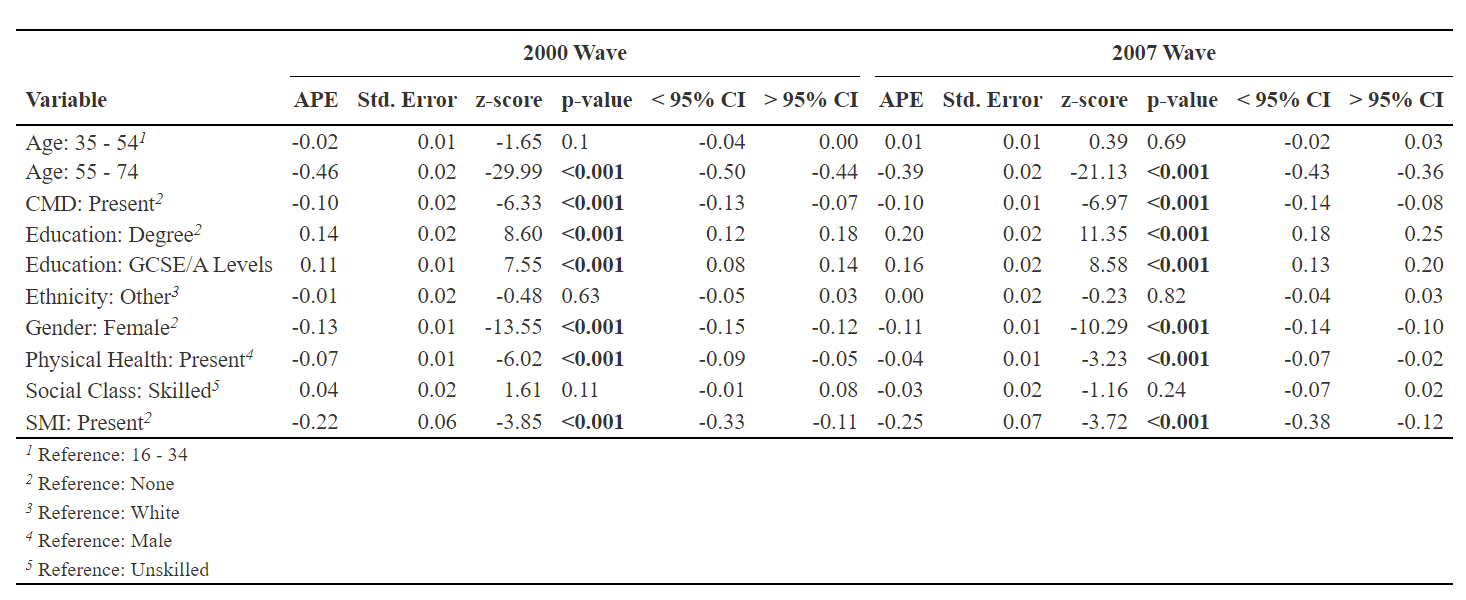
\includegraphics[width=460px,height=200px]{figure/apeecon} \caption[Average Partial Effects for Economic Activity]{Average Partial Effects for Economic Activity in 2000 and 2007}\label{fig:apeecon}
\end{figure}
Despite a great deal of similarity in results between the two waves, as expected, some differences are also apparent. The negative association between economic activity and being female, poor physical health, common mental disorders, and serious mental illness, is present in both years, but estimates for these factors are smaller in 2007 than in 2000. Additionally, there is also a negative association between age and economic activity, with the effect size being smaller in 2007 than in 2000 and more pronounced for those between the ages of 55-74 in 2000 than 2007.

These similarities suggest that the factors influencing economic activity have remained relatively consistent over time, with higher levels of education, good physical, and mental health, and being of a younger age being important for economic activity regardless of the specific year examined.

Interesting differences in social class emerge, with a larger positive effect of being skilled on economic activity in 2000 than in 2007. For example, those in the skilled category were 4\% more likely to be economically active in 2000, although this was not statistically significant. In contrast, in 2007 the third largest positive effect was for those aged between 35 and 54 years old, who were 1\% more likely to be employed than those aged 16 to 34 years old, although this also was not significant.

The difference in the economic conditions and the state of the labour market at the time might have been a factor in the differences. In 2000, the UK was amid an economic boom, and there may have been a high demand for skilled workers in certain industries. On the other hand, in 2007, the global fiscal crisis was beginning to take hold, and this may have affected employment opportunities for certain individuals. Age, education, and training can play a role in an individual's economic activity. Employers may be more likely to hire older, more experienced individuals with the skills and knowledge needed for the job, especially in certain industries.

Factors such as being female and aged between 55 and 74 years old have a large negative and statistically significant effect on being economically active. Females were 13\% less likely to be economically active in 2000 and 11\% less likely in 2007 than males. The trend could be due to historic discrimination faced by women in the job market, especially those who have had less access to education and training opportunities. This can impact employment prospects and make it more difficult to find or maintain that employment. Some women may have chosen to leave the labour force or reduce their hours in order to care for children or elderly family members.

It's important to note that while certain groups of people may have had an advantage in the job market at a particular time, this does not necessarily mean that they will always have an advantage, as the labour market can change over time, and the skills and experiences that are in demand can also shift.




\begin{figure}
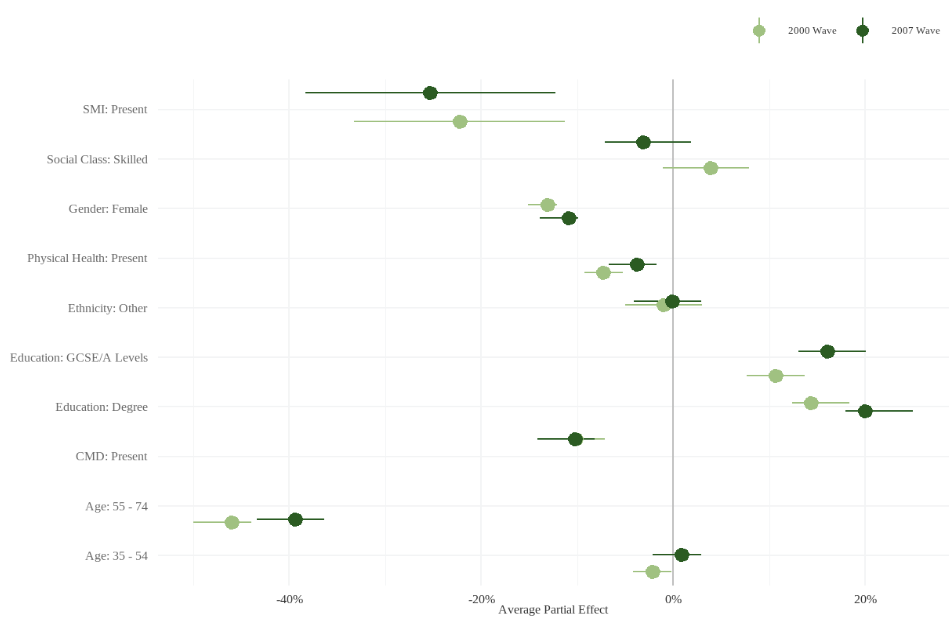
\includegraphics[width=450px,height=300px]{figure/apeeconp} \caption[Average Partial Effects Plot for Economic Activity]{Average Partial Effects Plot for Economic Activity in 2000 and 2007}\label{fig:apeeconp}
\end{figure}
\hypertarget{goodness-of-fit-for-economic-activity}{%
\subsection{Goodness of Fit for Economic Activity}\label{goodness-of-fit-for-economic-activity}}

Figure \ref{fig:gofecon} shows the results of diagnostic tests for the models applied to each survey wave. McFadden's pseudo R2 statistic is a measure of the goodness-of-fit of the model and is used to assess how well the model is able to explain the variation in the data. A value closer to 1 indicates a better fit of the model, while a value closer to 0 indicates a poor fit. The value of the McFadden's pseudo R2 statistic ranges from 0.26 for the model applied to the 2000 survey wave to 0.24 for the model applied to the 2007 survey wave.

A value of 0.26 for the model applied to the 2000 survey wave and 0.24 for the model applied to the 2007 survey wave suggests that the model has a relatively good fit, as it is able to explain a significant amount of the variation in the data. The small difference between the two values indicates that the fit of the models for both survey waves is quite similar.




\begin{figure}
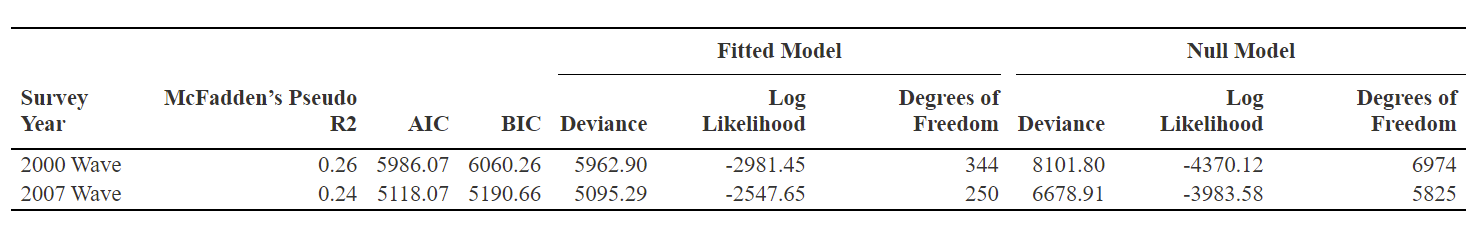
\includegraphics[width=460px,height=100px]{figure/gofecon} \caption[Goodness of Fit for Economic Activity Models]{Goodness of Fit for Economic Activity Models in 2000 and 2007}\label{fig:gofecon}
\end{figure}
\hypertarget{employment-status-1}{%
\section{Employment Status}\label{employment-status-1}}

This section covers results of logistic regression models applied to employment status of those who were economically active (unemployed or employed). In effect, this model nests inside the first. Having identified factors which lead to people being more or less likely to be economically active rather than inactive, we now focus only on those who are active, and model the factors which make them more or less likely to be in employment rather than unemployed. As before, two models are reported - one for each of the survey waves.

\hypertarget{model-results-for-employment-status}{%
\subsection{Model Results for Employment Status}\label{model-results-for-employment-status}}

There were 5,037 individuals included in the model for 2000 and 4,211 individuals in 2007 for employment status. Model results can be seen in Table \ref{tab:results2-empsmod}.

\providecommand{\huxb}[2]{\arrayrulecolor[RGB]{#1}\global\arrayrulewidth=#2pt}
  \providecommand{\huxvb}[2]{\color[RGB]{#1}\vrule width #2pt}
  \providecommand{\huxtpad}[1]{\rule{0pt}{#1}}
  \providecommand{\huxbpad}[1]{\rule[-#1]{0pt}{#1}}
\begin{table}[ht]
\begin{centerbox}
\begin{threeparttable}
 \setlength{\tabcolsep}{0pt}
\begin{adjustbox}{width=1\textwidth}
\normalsize
\begin{tabular}{l l l l l l l l l}


\hhline{>{\arrayrulecolor[RGB]{0, 0, 0}\global\arrayrulewidth=0.4pt}->{\arrayrulecolor[RGB]{0, 0, 0}\global\arrayrulewidth=0.4pt}->{\arrayrulecolor[RGB]{0, 0, 0}\global\arrayrulewidth=0.4pt}->{\arrayrulecolor[RGB]{0, 0, 0}\global\arrayrulewidth=0.4pt}->{\arrayrulecolor[RGB]{0, 0, 0}\global\arrayrulewidth=0.4pt}->{\arrayrulecolor[RGB]{0, 0, 0}\global\arrayrulewidth=0.4pt}->{\arrayrulecolor[RGB]{0, 0, 0}\global\arrayrulewidth=0.4pt}->{\arrayrulecolor[RGB]{0, 0, 0}\global\arrayrulewidth=0.4pt}->{\arrayrulecolor[RGB]{0, 0, 0}\global\arrayrulewidth=0.4pt}-}
\arrayrulecolor{black}

\multicolumn{1}{!{\color[RGB]{0, 0, 0}\vrule width 0pt}l!{\color[RGB]{0, 0, 0}\vrule width 0pt}}{\rule{0pt}{1pt + 1em}\raggedright \hspace{0pt} \textbf{{\fontsize{14pt}{16.8pt}\selectfont 
}} \hspace{1pt}\rule[-1pt]{0pt}{1pt}} &
\multicolumn{4}{c!{\color[RGB]{0, 0, 0}\vrule width 0pt}}{\rule{0pt}{1pt + 1em}\centering \hspace{1pt} \textbf{{\fontsize{14pt}{16.8pt}\selectfont \textbf{2000 Wave}
}} \hspace{1pt}\rule[-1pt]{0pt}{1pt}} &
\multicolumn{4}{c!{\color[RGB]{0, 0, 0}\vrule width 0pt}}{\rule{0pt}{1pt + 1em}\centering \hspace{1pt} \textbf{{\fontsize{14pt}{16.8pt}\selectfont \textbf{2007 Wave}
}} \hspace{1pt}\rule[-1pt]{0pt}{1pt}} \tabularnewline[-0.5pt]


\hhline{}
\arrayrulecolor{black}

\multicolumn{1}{!{\color[RGB]{0, 0, 0}\vrule width 0pt}l!{\color[RGB]{0, 0, 0}\vrule width 0pt}}{\rule{0pt}{1pt + 1em}\raggedright \hspace{0pt} \textbf{{\fontsize{14pt}{16.8pt}\selectfont \textbf{Variable}
}} \hspace{1pt}\rule[-1pt]{0pt}{1pt}} &
\multicolumn{1}{c!{\color[RGB]{0, 0, 0}\vrule width 0pt}}{\rule{0pt}{1pt + 1em}\centering \hspace{1pt} \textbf{{\fontsize{14pt}{16.8pt}\selectfont \textbf{N}
}} \hspace{1pt}\rule[-1pt]{0pt}{1pt}} &
\multicolumn{1}{c!{\color[RGB]{0, 0, 0}\vrule width 0pt}}{\rule{0pt}{1pt + 1em}\centering \hspace{1pt} \textbf{{\fontsize{14pt}{16.8pt}\selectfont \textbf{OR}
}} \hspace{1pt}\rule[-1pt]{0pt}{1pt}} &
\multicolumn{1}{c!{\color[RGB]{0, 0, 0}\vrule width 0pt}}{\rule{0pt}{1pt + 1em}\centering \hspace{1pt} \textbf{{\fontsize{14pt}{16.8pt}\selectfont \textbf{95\% CI}
}} \hspace{1pt}\rule[-1pt]{0pt}{1pt}} &
\multicolumn{1}{c!{\color[RGB]{0, 0, 0}\vrule width 0pt}}{\rule{0pt}{1pt + 1em}\centering \hspace{1pt} \textbf{{\fontsize{14pt}{16.8pt}\selectfont \textbf{p-value}
}} \hspace{1pt}\rule[-1pt]{0pt}{1pt}} &
\multicolumn{1}{c!{\color[RGB]{0, 0, 0}\vrule width 0pt}}{\rule{0pt}{1pt + 1em}\centering \hspace{1pt} \textbf{{\fontsize{14pt}{16.8pt}\selectfont \textbf{N}
}} \hspace{1pt}\rule[-1pt]{0pt}{1pt}} &
\multicolumn{1}{c!{\color[RGB]{0, 0, 0}\vrule width 0pt}}{\rule{0pt}{1pt + 1em}\centering \hspace{1pt} \textbf{{\fontsize{14pt}{16.8pt}\selectfont \textbf{OR}
}} \hspace{1pt}\rule[-1pt]{0pt}{1pt}} &
\multicolumn{1}{c!{\color[RGB]{0, 0, 0}\vrule width 0pt}}{\rule{0pt}{1pt + 1em}\centering \hspace{1pt} \textbf{{\fontsize{14pt}{16.8pt}\selectfont \textbf{95\% CI}
}} \hspace{1pt}\rule[-1pt]{0pt}{1pt}} &
\multicolumn{1}{c!{\color[RGB]{0, 0, 0}\vrule width 0pt}}{\rule{0pt}{1pt + 1em}\centering \hspace{1pt} \textbf{{\fontsize{14pt}{16.8pt}\selectfont \textbf{p-value}
}} \hspace{0pt}\rule[-1pt]{0pt}{1pt}} \tabularnewline[-0.5pt]


\hhline{>{\arrayrulecolor[RGB]{0, 0, 0}\global\arrayrulewidth=0.4pt}->{\arrayrulecolor[RGB]{0, 0, 0}\global\arrayrulewidth=0.4pt}->{\arrayrulecolor[RGB]{0, 0, 0}\global\arrayrulewidth=0.4pt}->{\arrayrulecolor[RGB]{0, 0, 0}\global\arrayrulewidth=0.4pt}->{\arrayrulecolor[RGB]{0, 0, 0}\global\arrayrulewidth=0.4pt}->{\arrayrulecolor[RGB]{0, 0, 0}\global\arrayrulewidth=0.4pt}->{\arrayrulecolor[RGB]{0, 0, 0}\global\arrayrulewidth=0.4pt}->{\arrayrulecolor[RGB]{0, 0, 0}\global\arrayrulewidth=0.4pt}->{\arrayrulecolor[RGB]{0, 0, 0}\global\arrayrulewidth=0.4pt}-}
\arrayrulecolor{black}

\multicolumn{1}{!{\color[RGB]{0, 0, 0}\vrule width 0pt}l!{\color[RGB]{0, 0, 0}\vrule width 0pt}}{\rule{0pt}{1pt + 1em}\raggedright \hspace{0pt} \textbf{{\fontsize{14pt}{16.8pt}\selectfont Gender}} \hspace{1pt}\rule[-1pt]{0pt}{1pt}} &
\multicolumn{1}{c!{\color[RGB]{0, 0, 0}\vrule width 0pt}}{\rule{0pt}{1pt + 1em}\centering \hspace{1pt} {\fontsize{14pt}{16.8pt}\selectfont 5,037} \hspace{1pt}\rule[-1pt]{0pt}{1pt}} &
\multicolumn{1}{c!{\color[RGB]{0, 0, 0}\vrule width 0pt}}{\rule{0pt}{1pt + 1em}\centering \hspace{1pt} {\fontsize{14pt}{16.8pt}\selectfont } \hspace{1pt}\rule[-1pt]{0pt}{1pt}} &
\multicolumn{1}{c!{\color[RGB]{0, 0, 0}\vrule width 0pt}}{\rule{0pt}{1pt + 1em}\centering \hspace{1pt} {\fontsize{14pt}{16.8pt}\selectfont } \hspace{1pt}\rule[-1pt]{0pt}{1pt}} &
\multicolumn{1}{c!{\color[RGB]{0, 0, 0}\vrule width 0pt}}{\rule{0pt}{1pt + 1em}\centering \hspace{1pt} {\fontsize{14pt}{16.8pt}\selectfont } \hspace{1pt}\rule[-1pt]{0pt}{1pt}} &
\multicolumn{1}{c!{\color[RGB]{0, 0, 0}\vrule width 0pt}}{\rule{0pt}{1pt + 1em}\centering \hspace{1pt} {\fontsize{14pt}{16.8pt}\selectfont 4,211} \hspace{1pt}\rule[-1pt]{0pt}{1pt}} &
\multicolumn{1}{c!{\color[RGB]{0, 0, 0}\vrule width 0pt}}{\rule{0pt}{1pt + 1em}\centering \hspace{1pt} {\fontsize{14pt}{16.8pt}\selectfont } \hspace{1pt}\rule[-1pt]{0pt}{1pt}} &
\multicolumn{1}{c!{\color[RGB]{0, 0, 0}\vrule width 0pt}}{\rule{0pt}{1pt + 1em}\centering \hspace{1pt} {\fontsize{14pt}{16.8pt}\selectfont } \hspace{1pt}\rule[-1pt]{0pt}{1pt}} &
\multicolumn{1}{c!{\color[RGB]{0, 0, 0}\vrule width 0pt}}{\rule{0pt}{1pt + 1em}\centering \hspace{1pt} {\fontsize{14pt}{16.8pt}\selectfont } \hspace{0pt}\rule[-1pt]{0pt}{1pt}} \tabularnewline[-0.5pt]


\hhline{}
\arrayrulecolor{black}

\multicolumn{1}{!{\color[RGB]{0, 0, 0}\vrule width 0pt}l!{\color[RGB]{0, 0, 0}\vrule width 0pt}}{\rule{0pt}{1pt + 1em}\raggedright \hspace{0pt} {\fontsize{14pt}{16.8pt}\selectfont Male} \hspace{1pt}\rule[-1pt]{0pt}{1pt}} &
\multicolumn{1}{c!{\color[RGB]{0, 0, 0}\vrule width 0pt}}{\rule{0pt}{1pt + 1em}\centering \hspace{1pt} {\fontsize{14pt}{16.8pt}\selectfont } \hspace{1pt}\rule[-1pt]{0pt}{1pt}} &
\multicolumn{1}{c!{\color[RGB]{0, 0, 0}\vrule width 0pt}}{\rule{0pt}{1pt + 1em}\centering \hspace{1pt} {\fontsize{14pt}{16.8pt}\selectfont —} \hspace{1pt}\rule[-1pt]{0pt}{1pt}} &
\multicolumn{1}{c!{\color[RGB]{0, 0, 0}\vrule width 0pt}}{\rule{0pt}{1pt + 1em}\centering \hspace{1pt} {\fontsize{14pt}{16.8pt}\selectfont —} \hspace{1pt}\rule[-1pt]{0pt}{1pt}} &
\multicolumn{1}{c!{\color[RGB]{0, 0, 0}\vrule width 0pt}}{\rule{0pt}{1pt + 1em}\centering \hspace{1pt} {\fontsize{14pt}{16.8pt}\selectfont } \hspace{1pt}\rule[-1pt]{0pt}{1pt}} &
\multicolumn{1}{c!{\color[RGB]{0, 0, 0}\vrule width 0pt}}{\rule{0pt}{1pt + 1em}\centering \hspace{1pt} {\fontsize{14pt}{16.8pt}\selectfont } \hspace{1pt}\rule[-1pt]{0pt}{1pt}} &
\multicolumn{1}{c!{\color[RGB]{0, 0, 0}\vrule width 0pt}}{\rule{0pt}{1pt + 1em}\centering \hspace{1pt} {\fontsize{14pt}{16.8pt}\selectfont —} \hspace{1pt}\rule[-1pt]{0pt}{1pt}} &
\multicolumn{1}{c!{\color[RGB]{0, 0, 0}\vrule width 0pt}}{\rule{0pt}{1pt + 1em}\centering \hspace{1pt} {\fontsize{14pt}{16.8pt}\selectfont —} \hspace{1pt}\rule[-1pt]{0pt}{1pt}} &
\multicolumn{1}{c!{\color[RGB]{0, 0, 0}\vrule width 0pt}}{\rule{0pt}{1pt + 1em}\centering \hspace{1pt} {\fontsize{14pt}{16.8pt}\selectfont } \hspace{0pt}\rule[-1pt]{0pt}{1pt}} \tabularnewline[-0.5pt]


\hhline{}
\arrayrulecolor{black}

\multicolumn{1}{!{\color[RGB]{0, 0, 0}\vrule width 0pt}l!{\color[RGB]{0, 0, 0}\vrule width 0pt}}{\rule{0pt}{1pt + 1em}\raggedright \hspace{0pt} {\fontsize{14pt}{16.8pt}\selectfont Female} \hspace{1pt}\rule[-1pt]{0pt}{1pt}} &
\multicolumn{1}{c!{\color[RGB]{0, 0, 0}\vrule width 0pt}}{\rule{0pt}{1pt + 1em}\centering \hspace{1pt} {\fontsize{14pt}{16.8pt}\selectfont } \hspace{1pt}\rule[-1pt]{0pt}{1pt}} &
\multicolumn{1}{c!{\color[RGB]{0, 0, 0}\vrule width 0pt}}{\rule{0pt}{1pt + 1em}\centering \hspace{1pt} {\fontsize{14pt}{16.8pt}\selectfont 1.21} \hspace{1pt}\rule[-1pt]{0pt}{1pt}} &
\multicolumn{1}{c!{\color[RGB]{0, 0, 0}\vrule width 0pt}}{\rule{0pt}{1pt + 1em}\centering \hspace{1pt} {\fontsize{14pt}{16.8pt}\selectfont 0.87, 1.67} \hspace{1pt}\rule[-1pt]{0pt}{1pt}} &
\multicolumn{1}{c!{\color[RGB]{0, 0, 0}\vrule width 0pt}}{\rule{0pt}{1pt + 1em}\centering \hspace{1pt} {\fontsize{14pt}{16.8pt}\selectfont 0.25} \hspace{1pt}\rule[-1pt]{0pt}{1pt}} &
\multicolumn{1}{c!{\color[RGB]{0, 0, 0}\vrule width 0pt}}{\rule{0pt}{1pt + 1em}\centering \hspace{1pt} {\fontsize{14pt}{16.8pt}\selectfont } \hspace{1pt}\rule[-1pt]{0pt}{1pt}} &
\multicolumn{1}{c!{\color[RGB]{0, 0, 0}\vrule width 0pt}}{\rule{0pt}{1pt + 1em}\centering \hspace{1pt} {\fontsize{14pt}{16.8pt}\selectfont 1.21} \hspace{1pt}\rule[-1pt]{0pt}{1pt}} &
\multicolumn{1}{c!{\color[RGB]{0, 0, 0}\vrule width 0pt}}{\rule{0pt}{1pt + 1em}\centering \hspace{1pt} {\fontsize{14pt}{16.8pt}\selectfont 0.80, 1.84} \hspace{1pt}\rule[-1pt]{0pt}{1pt}} &
\multicolumn{1}{c!{\color[RGB]{0, 0, 0}\vrule width 0pt}}{\rule{0pt}{1pt + 1em}\centering \hspace{1pt} {\fontsize{14pt}{16.8pt}\selectfont 0.37} \hspace{0pt}\rule[-1pt]{0pt}{1pt}} \tabularnewline[-0.5pt]


\hhline{}
\arrayrulecolor{black}

\multicolumn{1}{!{\color[RGB]{0, 0, 0}\vrule width 0pt}l!{\color[RGB]{0, 0, 0}\vrule width 0pt}}{\rule{0pt}{1pt + 1em}\raggedright \hspace{0pt} \textbf{{\fontsize{14pt}{16.8pt}\selectfont Age Band}} \hspace{1pt}\rule[-1pt]{0pt}{1pt}} &
\multicolumn{1}{c!{\color[RGB]{0, 0, 0}\vrule width 0pt}}{\rule{0pt}{1pt + 1em}\centering \hspace{1pt} {\fontsize{14pt}{16.8pt}\selectfont 5,037} \hspace{1pt}\rule[-1pt]{0pt}{1pt}} &
\multicolumn{1}{c!{\color[RGB]{0, 0, 0}\vrule width 0pt}}{\rule{0pt}{1pt + 1em}\centering \hspace{1pt} {\fontsize{14pt}{16.8pt}\selectfont } \hspace{1pt}\rule[-1pt]{0pt}{1pt}} &
\multicolumn{1}{c!{\color[RGB]{0, 0, 0}\vrule width 0pt}}{\rule{0pt}{1pt + 1em}\centering \hspace{1pt} {\fontsize{14pt}{16.8pt}\selectfont } \hspace{1pt}\rule[-1pt]{0pt}{1pt}} &
\multicolumn{1}{c!{\color[RGB]{0, 0, 0}\vrule width 0pt}}{\rule{0pt}{1pt + 1em}\centering \hspace{1pt} {\fontsize{14pt}{16.8pt}\selectfont } \hspace{1pt}\rule[-1pt]{0pt}{1pt}} &
\multicolumn{1}{c!{\color[RGB]{0, 0, 0}\vrule width 0pt}}{\rule{0pt}{1pt + 1em}\centering \hspace{1pt} {\fontsize{14pt}{16.8pt}\selectfont 4,211} \hspace{1pt}\rule[-1pt]{0pt}{1pt}} &
\multicolumn{1}{c!{\color[RGB]{0, 0, 0}\vrule width 0pt}}{\rule{0pt}{1pt + 1em}\centering \hspace{1pt} {\fontsize{14pt}{16.8pt}\selectfont } \hspace{1pt}\rule[-1pt]{0pt}{1pt}} &
\multicolumn{1}{c!{\color[RGB]{0, 0, 0}\vrule width 0pt}}{\rule{0pt}{1pt + 1em}\centering \hspace{1pt} {\fontsize{14pt}{16.8pt}\selectfont } \hspace{1pt}\rule[-1pt]{0pt}{1pt}} &
\multicolumn{1}{c!{\color[RGB]{0, 0, 0}\vrule width 0pt}}{\rule{0pt}{1pt + 1em}\centering \hspace{1pt} {\fontsize{14pt}{16.8pt}\selectfont } \hspace{0pt}\rule[-1pt]{0pt}{1pt}} \tabularnewline[-0.5pt]


\hhline{}
\arrayrulecolor{black}

\multicolumn{1}{!{\color[RGB]{0, 0, 0}\vrule width 0pt}l!{\color[RGB]{0, 0, 0}\vrule width 0pt}}{\rule{0pt}{1pt + 1em}\raggedright \hspace{0pt} {\fontsize{14pt}{16.8pt}\selectfont 16 - 34} \hspace{1pt}\rule[-1pt]{0pt}{1pt}} &
\multicolumn{1}{c!{\color[RGB]{0, 0, 0}\vrule width 0pt}}{\rule{0pt}{1pt + 1em}\centering \hspace{1pt} {\fontsize{14pt}{16.8pt}\selectfont } \hspace{1pt}\rule[-1pt]{0pt}{1pt}} &
\multicolumn{1}{c!{\color[RGB]{0, 0, 0}\vrule width 0pt}}{\rule{0pt}{1pt + 1em}\centering \hspace{1pt} {\fontsize{14pt}{16.8pt}\selectfont —} \hspace{1pt}\rule[-1pt]{0pt}{1pt}} &
\multicolumn{1}{c!{\color[RGB]{0, 0, 0}\vrule width 0pt}}{\rule{0pt}{1pt + 1em}\centering \hspace{1pt} {\fontsize{14pt}{16.8pt}\selectfont —} \hspace{1pt}\rule[-1pt]{0pt}{1pt}} &
\multicolumn{1}{c!{\color[RGB]{0, 0, 0}\vrule width 0pt}}{\rule{0pt}{1pt + 1em}\centering \hspace{1pt} {\fontsize{14pt}{16.8pt}\selectfont } \hspace{1pt}\rule[-1pt]{0pt}{1pt}} &
\multicolumn{1}{c!{\color[RGB]{0, 0, 0}\vrule width 0pt}}{\rule{0pt}{1pt + 1em}\centering \hspace{1pt} {\fontsize{14pt}{16.8pt}\selectfont } \hspace{1pt}\rule[-1pt]{0pt}{1pt}} &
\multicolumn{1}{c!{\color[RGB]{0, 0, 0}\vrule width 0pt}}{\rule{0pt}{1pt + 1em}\centering \hspace{1pt} {\fontsize{14pt}{16.8pt}\selectfont —} \hspace{1pt}\rule[-1pt]{0pt}{1pt}} &
\multicolumn{1}{c!{\color[RGB]{0, 0, 0}\vrule width 0pt}}{\rule{0pt}{1pt + 1em}\centering \hspace{1pt} {\fontsize{14pt}{16.8pt}\selectfont —} \hspace{1pt}\rule[-1pt]{0pt}{1pt}} &
\multicolumn{1}{c!{\color[RGB]{0, 0, 0}\vrule width 0pt}}{\rule{0pt}{1pt + 1em}\centering \hspace{1pt} {\fontsize{14pt}{16.8pt}\selectfont } \hspace{0pt}\rule[-1pt]{0pt}{1pt}} \tabularnewline[-0.5pt]


\hhline{}
\arrayrulecolor{black}

\multicolumn{1}{!{\color[RGB]{0, 0, 0}\vrule width 0pt}l!{\color[RGB]{0, 0, 0}\vrule width 0pt}}{\rule{0pt}{1pt + 1em}\raggedright \hspace{0pt} {\fontsize{14pt}{16.8pt}\selectfont 35 - 54} \hspace{1pt}\rule[-1pt]{0pt}{1pt}} &
\multicolumn{1}{c!{\color[RGB]{0, 0, 0}\vrule width 0pt}}{\rule{0pt}{1pt + 1em}\centering \hspace{1pt} {\fontsize{14pt}{16.8pt}\selectfont } \hspace{1pt}\rule[-1pt]{0pt}{1pt}} &
\multicolumn{1}{c!{\color[RGB]{0, 0, 0}\vrule width 0pt}}{\rule{0pt}{1pt + 1em}\centering \hspace{1pt} {\fontsize{14pt}{16.8pt}\selectfont 1.08} \hspace{1pt}\rule[-1pt]{0pt}{1pt}} &
\multicolumn{1}{c!{\color[RGB]{0, 0, 0}\vrule width 0pt}}{\rule{0pt}{1pt + 1em}\centering \hspace{1pt} {\fontsize{14pt}{16.8pt}\selectfont 0.74, 1.58} \hspace{1pt}\rule[-1pt]{0pt}{1pt}} &
\multicolumn{1}{c!{\color[RGB]{0, 0, 0}\vrule width 0pt}}{\rule{0pt}{1pt + 1em}\centering \hspace{1pt} {\fontsize{14pt}{16.8pt}\selectfont 0.68} \hspace{1pt}\rule[-1pt]{0pt}{1pt}} &
\multicolumn{1}{c!{\color[RGB]{0, 0, 0}\vrule width 0pt}}{\rule{0pt}{1pt + 1em}\centering \hspace{1pt} {\fontsize{14pt}{16.8pt}\selectfont } \hspace{1pt}\rule[-1pt]{0pt}{1pt}} &
\multicolumn{1}{c!{\color[RGB]{0, 0, 0}\vrule width 0pt}}{\rule{0pt}{1pt + 1em}\centering \hspace{1pt} {\fontsize{14pt}{16.8pt}\selectfont 1.63} \hspace{1pt}\rule[-1pt]{0pt}{1pt}} &
\multicolumn{1}{c!{\color[RGB]{0, 0, 0}\vrule width 0pt}}{\rule{0pt}{1pt + 1em}\centering \hspace{1pt} {\fontsize{14pt}{16.8pt}\selectfont 1.08, 2.48} \hspace{1pt}\rule[-1pt]{0pt}{1pt}} &
\multicolumn{1}{c!{\color[RGB]{0, 0, 0}\vrule width 0pt}}{\rule{0pt}{1pt + 1em}\centering \hspace{1pt} \textbf{{\fontsize{14pt}{16.8pt}\selectfont 0.021}} \hspace{0pt}\rule[-1pt]{0pt}{1pt}} \tabularnewline[-0.5pt]


\hhline{}
\arrayrulecolor{black}

\multicolumn{1}{!{\color[RGB]{0, 0, 0}\vrule width 0pt}l!{\color[RGB]{0, 0, 0}\vrule width 0pt}}{\rule{0pt}{1pt + 1em}\raggedright \hspace{0pt} {\fontsize{14pt}{16.8pt}\selectfont 55 - 74} \hspace{1pt}\rule[-1pt]{0pt}{1pt}} &
\multicolumn{1}{c!{\color[RGB]{0, 0, 0}\vrule width 0pt}}{\rule{0pt}{1pt + 1em}\centering \hspace{1pt} {\fontsize{14pt}{16.8pt}\selectfont } \hspace{1pt}\rule[-1pt]{0pt}{1pt}} &
\multicolumn{1}{c!{\color[RGB]{0, 0, 0}\vrule width 0pt}}{\rule{0pt}{1pt + 1em}\centering \hspace{1pt} {\fontsize{14pt}{16.8pt}\selectfont 0.97} \hspace{1pt}\rule[-1pt]{0pt}{1pt}} &
\multicolumn{1}{c!{\color[RGB]{0, 0, 0}\vrule width 0pt}}{\rule{0pt}{1pt + 1em}\centering \hspace{1pt} {\fontsize{14pt}{16.8pt}\selectfont 0.56, 1.68} \hspace{1pt}\rule[-1pt]{0pt}{1pt}} &
\multicolumn{1}{c!{\color[RGB]{0, 0, 0}\vrule width 0pt}}{\rule{0pt}{1pt + 1em}\centering \hspace{1pt} {\fontsize{14pt}{16.8pt}\selectfont 0.91} \hspace{1pt}\rule[-1pt]{0pt}{1pt}} &
\multicolumn{1}{c!{\color[RGB]{0, 0, 0}\vrule width 0pt}}{\rule{0pt}{1pt + 1em}\centering \hspace{1pt} {\fontsize{14pt}{16.8pt}\selectfont } \hspace{1pt}\rule[-1pt]{0pt}{1pt}} &
\multicolumn{1}{c!{\color[RGB]{0, 0, 0}\vrule width 0pt}}{\rule{0pt}{1pt + 1em}\centering \hspace{1pt} {\fontsize{14pt}{16.8pt}\selectfont 4.86} \hspace{1pt}\rule[-1pt]{0pt}{1pt}} &
\multicolumn{1}{c!{\color[RGB]{0, 0, 0}\vrule width 0pt}}{\rule{0pt}{1pt + 1em}\centering \hspace{1pt} {\fontsize{14pt}{16.8pt}\selectfont 2.12, 11.2} \hspace{1pt}\rule[-1pt]{0pt}{1pt}} &
\multicolumn{1}{c!{\color[RGB]{0, 0, 0}\vrule width 0pt}}{\rule{0pt}{1pt + 1em}\centering \hspace{1pt} \textbf{{\fontsize{14pt}{16.8pt}\selectfont $<$0.001}} \hspace{0pt}\rule[-1pt]{0pt}{1pt}} \tabularnewline[-0.5pt]


\hhline{}
\arrayrulecolor{black}

\multicolumn{1}{!{\color[RGB]{0, 0, 0}\vrule width 0pt}l!{\color[RGB]{0, 0, 0}\vrule width 0pt}}{\rule{0pt}{1pt + 1em}\raggedright \hspace{0pt} \textbf{{\fontsize{14pt}{16.8pt}\selectfont Ethnicity}} \hspace{1pt}\rule[-1pt]{0pt}{1pt}} &
\multicolumn{1}{c!{\color[RGB]{0, 0, 0}\vrule width 0pt}}{\rule{0pt}{1pt + 1em}\centering \hspace{1pt} {\fontsize{14pt}{16.8pt}\selectfont 5,037} \hspace{1pt}\rule[-1pt]{0pt}{1pt}} &
\multicolumn{1}{c!{\color[RGB]{0, 0, 0}\vrule width 0pt}}{\rule{0pt}{1pt + 1em}\centering \hspace{1pt} {\fontsize{14pt}{16.8pt}\selectfont } \hspace{1pt}\rule[-1pt]{0pt}{1pt}} &
\multicolumn{1}{c!{\color[RGB]{0, 0, 0}\vrule width 0pt}}{\rule{0pt}{1pt + 1em}\centering \hspace{1pt} {\fontsize{14pt}{16.8pt}\selectfont } \hspace{1pt}\rule[-1pt]{0pt}{1pt}} &
\multicolumn{1}{c!{\color[RGB]{0, 0, 0}\vrule width 0pt}}{\rule{0pt}{1pt + 1em}\centering \hspace{1pt} {\fontsize{14pt}{16.8pt}\selectfont } \hspace{1pt}\rule[-1pt]{0pt}{1pt}} &
\multicolumn{1}{c!{\color[RGB]{0, 0, 0}\vrule width 0pt}}{\rule{0pt}{1pt + 1em}\centering \hspace{1pt} {\fontsize{14pt}{16.8pt}\selectfont 4,211} \hspace{1pt}\rule[-1pt]{0pt}{1pt}} &
\multicolumn{1}{c!{\color[RGB]{0, 0, 0}\vrule width 0pt}}{\rule{0pt}{1pt + 1em}\centering \hspace{1pt} {\fontsize{14pt}{16.8pt}\selectfont } \hspace{1pt}\rule[-1pt]{0pt}{1pt}} &
\multicolumn{1}{c!{\color[RGB]{0, 0, 0}\vrule width 0pt}}{\rule{0pt}{1pt + 1em}\centering \hspace{1pt} {\fontsize{14pt}{16.8pt}\selectfont } \hspace{1pt}\rule[-1pt]{0pt}{1pt}} &
\multicolumn{1}{c!{\color[RGB]{0, 0, 0}\vrule width 0pt}}{\rule{0pt}{1pt + 1em}\centering \hspace{1pt} {\fontsize{14pt}{16.8pt}\selectfont } \hspace{0pt}\rule[-1pt]{0pt}{1pt}} \tabularnewline[-0.5pt]


\hhline{}
\arrayrulecolor{black}

\multicolumn{1}{!{\color[RGB]{0, 0, 0}\vrule width 0pt}l!{\color[RGB]{0, 0, 0}\vrule width 0pt}}{\rule{0pt}{1pt + 1em}\raggedright \hspace{0pt} {\fontsize{14pt}{16.8pt}\selectfont White} \hspace{1pt}\rule[-1pt]{0pt}{1pt}} &
\multicolumn{1}{c!{\color[RGB]{0, 0, 0}\vrule width 0pt}}{\rule{0pt}{1pt + 1em}\centering \hspace{1pt} {\fontsize{14pt}{16.8pt}\selectfont } \hspace{1pt}\rule[-1pt]{0pt}{1pt}} &
\multicolumn{1}{c!{\color[RGB]{0, 0, 0}\vrule width 0pt}}{\rule{0pt}{1pt + 1em}\centering \hspace{1pt} {\fontsize{14pt}{16.8pt}\selectfont —} \hspace{1pt}\rule[-1pt]{0pt}{1pt}} &
\multicolumn{1}{c!{\color[RGB]{0, 0, 0}\vrule width 0pt}}{\rule{0pt}{1pt + 1em}\centering \hspace{1pt} {\fontsize{14pt}{16.8pt}\selectfont —} \hspace{1pt}\rule[-1pt]{0pt}{1pt}} &
\multicolumn{1}{c!{\color[RGB]{0, 0, 0}\vrule width 0pt}}{\rule{0pt}{1pt + 1em}\centering \hspace{1pt} {\fontsize{14pt}{16.8pt}\selectfont } \hspace{1pt}\rule[-1pt]{0pt}{1pt}} &
\multicolumn{1}{c!{\color[RGB]{0, 0, 0}\vrule width 0pt}}{\rule{0pt}{1pt + 1em}\centering \hspace{1pt} {\fontsize{14pt}{16.8pt}\selectfont } \hspace{1pt}\rule[-1pt]{0pt}{1pt}} &
\multicolumn{1}{c!{\color[RGB]{0, 0, 0}\vrule width 0pt}}{\rule{0pt}{1pt + 1em}\centering \hspace{1pt} {\fontsize{14pt}{16.8pt}\selectfont —} \hspace{1pt}\rule[-1pt]{0pt}{1pt}} &
\multicolumn{1}{c!{\color[RGB]{0, 0, 0}\vrule width 0pt}}{\rule{0pt}{1pt + 1em}\centering \hspace{1pt} {\fontsize{14pt}{16.8pt}\selectfont —} \hspace{1pt}\rule[-1pt]{0pt}{1pt}} &
\multicolumn{1}{c!{\color[RGB]{0, 0, 0}\vrule width 0pt}}{\rule{0pt}{1pt + 1em}\centering \hspace{1pt} {\fontsize{14pt}{16.8pt}\selectfont } \hspace{0pt}\rule[-1pt]{0pt}{1pt}} \tabularnewline[-0.5pt]


\hhline{}
\arrayrulecolor{black}

\multicolumn{1}{!{\color[RGB]{0, 0, 0}\vrule width 0pt}l!{\color[RGB]{0, 0, 0}\vrule width 0pt}}{\rule{0pt}{1pt + 1em}\raggedright \hspace{0pt} {\fontsize{14pt}{16.8pt}\selectfont Other} \hspace{1pt}\rule[-1pt]{0pt}{1pt}} &
\multicolumn{1}{c!{\color[RGB]{0, 0, 0}\vrule width 0pt}}{\rule{0pt}{1pt + 1em}\centering \hspace{1pt} {\fontsize{14pt}{16.8pt}\selectfont } \hspace{1pt}\rule[-1pt]{0pt}{1pt}} &
\multicolumn{1}{c!{\color[RGB]{0, 0, 0}\vrule width 0pt}}{\rule{0pt}{1pt + 1em}\centering \hspace{1pt} {\fontsize{14pt}{16.8pt}\selectfont 0.48} \hspace{1pt}\rule[-1pt]{0pt}{1pt}} &
\multicolumn{1}{c!{\color[RGB]{0, 0, 0}\vrule width 0pt}}{\rule{0pt}{1pt + 1em}\centering \hspace{1pt} {\fontsize{14pt}{16.8pt}\selectfont 0.30, 0.78} \hspace{1pt}\rule[-1pt]{0pt}{1pt}} &
\multicolumn{1}{c!{\color[RGB]{0, 0, 0}\vrule width 0pt}}{\rule{0pt}{1pt + 1em}\centering \hspace{1pt} \textbf{{\fontsize{14pt}{16.8pt}\selectfont 0.003}} \hspace{1pt}\rule[-1pt]{0pt}{1pt}} &
\multicolumn{1}{c!{\color[RGB]{0, 0, 0}\vrule width 0pt}}{\rule{0pt}{1pt + 1em}\centering \hspace{1pt} {\fontsize{14pt}{16.8pt}\selectfont } \hspace{1pt}\rule[-1pt]{0pt}{1pt}} &
\multicolumn{1}{c!{\color[RGB]{0, 0, 0}\vrule width 0pt}}{\rule{0pt}{1pt + 1em}\centering \hspace{1pt} {\fontsize{14pt}{16.8pt}\selectfont 1.19} \hspace{1pt}\rule[-1pt]{0pt}{1pt}} &
\multicolumn{1}{c!{\color[RGB]{0, 0, 0}\vrule width 0pt}}{\rule{0pt}{1pt + 1em}\centering \hspace{1pt} {\fontsize{14pt}{16.8pt}\selectfont 0.57, 2.51} \hspace{1pt}\rule[-1pt]{0pt}{1pt}} &
\multicolumn{1}{c!{\color[RGB]{0, 0, 0}\vrule width 0pt}}{\rule{0pt}{1pt + 1em}\centering \hspace{1pt} {\fontsize{14pt}{16.8pt}\selectfont 0.64} \hspace{0pt}\rule[-1pt]{0pt}{1pt}} \tabularnewline[-0.5pt]


\hhline{}
\arrayrulecolor{black}

\multicolumn{1}{!{\color[RGB]{0, 0, 0}\vrule width 0pt}l!{\color[RGB]{0, 0, 0}\vrule width 0pt}}{\rule{0pt}{1pt + 1em}\raggedright \hspace{0pt} \textbf{{\fontsize{14pt}{16.8pt}\selectfont Social Class}} \hspace{1pt}\rule[-1pt]{0pt}{1pt}} &
\multicolumn{1}{c!{\color[RGB]{0, 0, 0}\vrule width 0pt}}{\rule{0pt}{1pt + 1em}\centering \hspace{1pt} {\fontsize{14pt}{16.8pt}\selectfont 5,037} \hspace{1pt}\rule[-1pt]{0pt}{1pt}} &
\multicolumn{1}{c!{\color[RGB]{0, 0, 0}\vrule width 0pt}}{\rule{0pt}{1pt + 1em}\centering \hspace{1pt} {\fontsize{14pt}{16.8pt}\selectfont } \hspace{1pt}\rule[-1pt]{0pt}{1pt}} &
\multicolumn{1}{c!{\color[RGB]{0, 0, 0}\vrule width 0pt}}{\rule{0pt}{1pt + 1em}\centering \hspace{1pt} {\fontsize{14pt}{16.8pt}\selectfont } \hspace{1pt}\rule[-1pt]{0pt}{1pt}} &
\multicolumn{1}{c!{\color[RGB]{0, 0, 0}\vrule width 0pt}}{\rule{0pt}{1pt + 1em}\centering \hspace{1pt} {\fontsize{14pt}{16.8pt}\selectfont } \hspace{1pt}\rule[-1pt]{0pt}{1pt}} &
\multicolumn{1}{c!{\color[RGB]{0, 0, 0}\vrule width 0pt}}{\rule{0pt}{1pt + 1em}\centering \hspace{1pt} {\fontsize{14pt}{16.8pt}\selectfont 4,211} \hspace{1pt}\rule[-1pt]{0pt}{1pt}} &
\multicolumn{1}{c!{\color[RGB]{0, 0, 0}\vrule width 0pt}}{\rule{0pt}{1pt + 1em}\centering \hspace{1pt} {\fontsize{14pt}{16.8pt}\selectfont } \hspace{1pt}\rule[-1pt]{0pt}{1pt}} &
\multicolumn{1}{c!{\color[RGB]{0, 0, 0}\vrule width 0pt}}{\rule{0pt}{1pt + 1em}\centering \hspace{1pt} {\fontsize{14pt}{16.8pt}\selectfont } \hspace{1pt}\rule[-1pt]{0pt}{1pt}} &
\multicolumn{1}{c!{\color[RGB]{0, 0, 0}\vrule width 0pt}}{\rule{0pt}{1pt + 1em}\centering \hspace{1pt} {\fontsize{14pt}{16.8pt}\selectfont } \hspace{0pt}\rule[-1pt]{0pt}{1pt}} \tabularnewline[-0.5pt]


\hhline{}
\arrayrulecolor{black}

\multicolumn{1}{!{\color[RGB]{0, 0, 0}\vrule width 0pt}l!{\color[RGB]{0, 0, 0}\vrule width 0pt}}{\rule{0pt}{1pt + 1em}\raggedright \hspace{0pt} {\fontsize{14pt}{16.8pt}\selectfont Unskilled} \hspace{1pt}\rule[-1pt]{0pt}{1pt}} &
\multicolumn{1}{c!{\color[RGB]{0, 0, 0}\vrule width 0pt}}{\rule{0pt}{1pt + 1em}\centering \hspace{1pt} {\fontsize{14pt}{16.8pt}\selectfont } \hspace{1pt}\rule[-1pt]{0pt}{1pt}} &
\multicolumn{1}{c!{\color[RGB]{0, 0, 0}\vrule width 0pt}}{\rule{0pt}{1pt + 1em}\centering \hspace{1pt} {\fontsize{14pt}{16.8pt}\selectfont —} \hspace{1pt}\rule[-1pt]{0pt}{1pt}} &
\multicolumn{1}{c!{\color[RGB]{0, 0, 0}\vrule width 0pt}}{\rule{0pt}{1pt + 1em}\centering \hspace{1pt} {\fontsize{14pt}{16.8pt}\selectfont —} \hspace{1pt}\rule[-1pt]{0pt}{1pt}} &
\multicolumn{1}{c!{\color[RGB]{0, 0, 0}\vrule width 0pt}}{\rule{0pt}{1pt + 1em}\centering \hspace{1pt} {\fontsize{14pt}{16.8pt}\selectfont } \hspace{1pt}\rule[-1pt]{0pt}{1pt}} &
\multicolumn{1}{c!{\color[RGB]{0, 0, 0}\vrule width 0pt}}{\rule{0pt}{1pt + 1em}\centering \hspace{1pt} {\fontsize{14pt}{16.8pt}\selectfont } \hspace{1pt}\rule[-1pt]{0pt}{1pt}} &
\multicolumn{1}{c!{\color[RGB]{0, 0, 0}\vrule width 0pt}}{\rule{0pt}{1pt + 1em}\centering \hspace{1pt} {\fontsize{14pt}{16.8pt}\selectfont —} \hspace{1pt}\rule[-1pt]{0pt}{1pt}} &
\multicolumn{1}{c!{\color[RGB]{0, 0, 0}\vrule width 0pt}}{\rule{0pt}{1pt + 1em}\centering \hspace{1pt} {\fontsize{14pt}{16.8pt}\selectfont —} \hspace{1pt}\rule[-1pt]{0pt}{1pt}} &
\multicolumn{1}{c!{\color[RGB]{0, 0, 0}\vrule width 0pt}}{\rule{0pt}{1pt + 1em}\centering \hspace{1pt} {\fontsize{14pt}{16.8pt}\selectfont } \hspace{0pt}\rule[-1pt]{0pt}{1pt}} \tabularnewline[-0.5pt]


\hhline{}
\arrayrulecolor{black}

\multicolumn{1}{!{\color[RGB]{0, 0, 0}\vrule width 0pt}l!{\color[RGB]{0, 0, 0}\vrule width 0pt}}{\rule{0pt}{1pt + 1em}\raggedright \hspace{0pt} {\fontsize{14pt}{16.8pt}\selectfont Skilled} \hspace{1pt}\rule[-1pt]{0pt}{1pt}} &
\multicolumn{1}{c!{\color[RGB]{0, 0, 0}\vrule width 0pt}}{\rule{0pt}{1pt + 1em}\centering \hspace{1pt} {\fontsize{14pt}{16.8pt}\selectfont } \hspace{1pt}\rule[-1pt]{0pt}{1pt}} &
\multicolumn{1}{c!{\color[RGB]{0, 0, 0}\vrule width 0pt}}{\rule{0pt}{1pt + 1em}\centering \hspace{1pt} {\fontsize{14pt}{16.8pt}\selectfont 1.47} \hspace{1pt}\rule[-1pt]{0pt}{1pt}} &
\multicolumn{1}{c!{\color[RGB]{0, 0, 0}\vrule width 0pt}}{\rule{0pt}{1pt + 1em}\centering \hspace{1pt} {\fontsize{14pt}{16.8pt}\selectfont 0.74, 2.94} \hspace{1pt}\rule[-1pt]{0pt}{1pt}} &
\multicolumn{1}{c!{\color[RGB]{0, 0, 0}\vrule width 0pt}}{\rule{0pt}{1pt + 1em}\centering \hspace{1pt} {\fontsize{14pt}{16.8pt}\selectfont 0.27} \hspace{1pt}\rule[-1pt]{0pt}{1pt}} &
\multicolumn{1}{c!{\color[RGB]{0, 0, 0}\vrule width 0pt}}{\rule{0pt}{1pt + 1em}\centering \hspace{1pt} {\fontsize{14pt}{16.8pt}\selectfont } \hspace{1pt}\rule[-1pt]{0pt}{1pt}} &
\multicolumn{1}{c!{\color[RGB]{0, 0, 0}\vrule width 0pt}}{\rule{0pt}{1pt + 1em}\centering \hspace{1pt} {\fontsize{14pt}{16.8pt}\selectfont 1.96} \hspace{1pt}\rule[-1pt]{0pt}{1pt}} &
\multicolumn{1}{c!{\color[RGB]{0, 0, 0}\vrule width 0pt}}{\rule{0pt}{1pt + 1em}\centering \hspace{1pt} {\fontsize{14pt}{16.8pt}\selectfont 0.95, 4.05} \hspace{1pt}\rule[-1pt]{0pt}{1pt}} &
\multicolumn{1}{c!{\color[RGB]{0, 0, 0}\vrule width 0pt}}{\rule{0pt}{1pt + 1em}\centering \hspace{1pt} {\fontsize{14pt}{16.8pt}\selectfont 0.068} \hspace{0pt}\rule[-1pt]{0pt}{1pt}} \tabularnewline[-0.5pt]


\hhline{}
\arrayrulecolor{black}

\multicolumn{1}{!{\color[RGB]{0, 0, 0}\vrule width 0pt}l!{\color[RGB]{0, 0, 0}\vrule width 0pt}}{\rule{0pt}{1pt + 1em}\raggedright \hspace{0pt} \textbf{{\fontsize{14pt}{16.8pt}\selectfont Education}} \hspace{1pt}\rule[-1pt]{0pt}{1pt}} &
\multicolumn{1}{c!{\color[RGB]{0, 0, 0}\vrule width 0pt}}{\rule{0pt}{1pt + 1em}\centering \hspace{1pt} {\fontsize{14pt}{16.8pt}\selectfont 5,037} \hspace{1pt}\rule[-1pt]{0pt}{1pt}} &
\multicolumn{1}{c!{\color[RGB]{0, 0, 0}\vrule width 0pt}}{\rule{0pt}{1pt + 1em}\centering \hspace{1pt} {\fontsize{14pt}{16.8pt}\selectfont } \hspace{1pt}\rule[-1pt]{0pt}{1pt}} &
\multicolumn{1}{c!{\color[RGB]{0, 0, 0}\vrule width 0pt}}{\rule{0pt}{1pt + 1em}\centering \hspace{1pt} {\fontsize{14pt}{16.8pt}\selectfont } \hspace{1pt}\rule[-1pt]{0pt}{1pt}} &
\multicolumn{1}{c!{\color[RGB]{0, 0, 0}\vrule width 0pt}}{\rule{0pt}{1pt + 1em}\centering \hspace{1pt} {\fontsize{14pt}{16.8pt}\selectfont } \hspace{1pt}\rule[-1pt]{0pt}{1pt}} &
\multicolumn{1}{c!{\color[RGB]{0, 0, 0}\vrule width 0pt}}{\rule{0pt}{1pt + 1em}\centering \hspace{1pt} {\fontsize{14pt}{16.8pt}\selectfont 4,211} \hspace{1pt}\rule[-1pt]{0pt}{1pt}} &
\multicolumn{1}{c!{\color[RGB]{0, 0, 0}\vrule width 0pt}}{\rule{0pt}{1pt + 1em}\centering \hspace{1pt} {\fontsize{14pt}{16.8pt}\selectfont } \hspace{1pt}\rule[-1pt]{0pt}{1pt}} &
\multicolumn{1}{c!{\color[RGB]{0, 0, 0}\vrule width 0pt}}{\rule{0pt}{1pt + 1em}\centering \hspace{1pt} {\fontsize{14pt}{16.8pt}\selectfont } \hspace{1pt}\rule[-1pt]{0pt}{1pt}} &
\multicolumn{1}{c!{\color[RGB]{0, 0, 0}\vrule width 0pt}}{\rule{0pt}{1pt + 1em}\centering \hspace{1pt} {\fontsize{14pt}{16.8pt}\selectfont } \hspace{0pt}\rule[-1pt]{0pt}{1pt}} \tabularnewline[-0.5pt]


\hhline{}
\arrayrulecolor{black}

\multicolumn{1}{!{\color[RGB]{0, 0, 0}\vrule width 0pt}l!{\color[RGB]{0, 0, 0}\vrule width 0pt}}{\rule{0pt}{1pt + 1em}\raggedright \hspace{0pt} {\fontsize{14pt}{16.8pt}\selectfont None} \hspace{1pt}\rule[-1pt]{0pt}{1pt}} &
\multicolumn{1}{c!{\color[RGB]{0, 0, 0}\vrule width 0pt}}{\rule{0pt}{1pt + 1em}\centering \hspace{1pt} {\fontsize{14pt}{16.8pt}\selectfont } \hspace{1pt}\rule[-1pt]{0pt}{1pt}} &
\multicolumn{1}{c!{\color[RGB]{0, 0, 0}\vrule width 0pt}}{\rule{0pt}{1pt + 1em}\centering \hspace{1pt} {\fontsize{14pt}{16.8pt}\selectfont —} \hspace{1pt}\rule[-1pt]{0pt}{1pt}} &
\multicolumn{1}{c!{\color[RGB]{0, 0, 0}\vrule width 0pt}}{\rule{0pt}{1pt + 1em}\centering \hspace{1pt} {\fontsize{14pt}{16.8pt}\selectfont —} \hspace{1pt}\rule[-1pt]{0pt}{1pt}} &
\multicolumn{1}{c!{\color[RGB]{0, 0, 0}\vrule width 0pt}}{\rule{0pt}{1pt + 1em}\centering \hspace{1pt} {\fontsize{14pt}{16.8pt}\selectfont } \hspace{1pt}\rule[-1pt]{0pt}{1pt}} &
\multicolumn{1}{c!{\color[RGB]{0, 0, 0}\vrule width 0pt}}{\rule{0pt}{1pt + 1em}\centering \hspace{1pt} {\fontsize{14pt}{16.8pt}\selectfont } \hspace{1pt}\rule[-1pt]{0pt}{1pt}} &
\multicolumn{1}{c!{\color[RGB]{0, 0, 0}\vrule width 0pt}}{\rule{0pt}{1pt + 1em}\centering \hspace{1pt} {\fontsize{14pt}{16.8pt}\selectfont —} \hspace{1pt}\rule[-1pt]{0pt}{1pt}} &
\multicolumn{1}{c!{\color[RGB]{0, 0, 0}\vrule width 0pt}}{\rule{0pt}{1pt + 1em}\centering \hspace{1pt} {\fontsize{14pt}{16.8pt}\selectfont —} \hspace{1pt}\rule[-1pt]{0pt}{1pt}} &
\multicolumn{1}{c!{\color[RGB]{0, 0, 0}\vrule width 0pt}}{\rule{0pt}{1pt + 1em}\centering \hspace{1pt} {\fontsize{14pt}{16.8pt}\selectfont } \hspace{0pt}\rule[-1pt]{0pt}{1pt}} \tabularnewline[-0.5pt]


\hhline{}
\arrayrulecolor{black}

\multicolumn{1}{!{\color[RGB]{0, 0, 0}\vrule width 0pt}l!{\color[RGB]{0, 0, 0}\vrule width 0pt}}{\rule{0pt}{1pt + 1em}\raggedright \hspace{0pt} {\fontsize{14pt}{16.8pt}\selectfont GCSE/A Levels} \hspace{1pt}\rule[-1pt]{0pt}{1pt}} &
\multicolumn{1}{c!{\color[RGB]{0, 0, 0}\vrule width 0pt}}{\rule{0pt}{1pt + 1em}\centering \hspace{1pt} {\fontsize{14pt}{16.8pt}\selectfont } \hspace{1pt}\rule[-1pt]{0pt}{1pt}} &
\multicolumn{1}{c!{\color[RGB]{0, 0, 0}\vrule width 0pt}}{\rule{0pt}{1pt + 1em}\centering \hspace{1pt} {\fontsize{14pt}{16.8pt}\selectfont 1.63} \hspace{1pt}\rule[-1pt]{0pt}{1pt}} &
\multicolumn{1}{c!{\color[RGB]{0, 0, 0}\vrule width 0pt}}{\rule{0pt}{1pt + 1em}\centering \hspace{1pt} {\fontsize{14pt}{16.8pt}\selectfont 1.08, 2.47} \hspace{1pt}\rule[-1pt]{0pt}{1pt}} &
\multicolumn{1}{c!{\color[RGB]{0, 0, 0}\vrule width 0pt}}{\rule{0pt}{1pt + 1em}\centering \hspace{1pt} \textbf{{\fontsize{14pt}{16.8pt}\selectfont 0.021}} \hspace{1pt}\rule[-1pt]{0pt}{1pt}} &
\multicolumn{1}{c!{\color[RGB]{0, 0, 0}\vrule width 0pt}}{\rule{0pt}{1pt + 1em}\centering \hspace{1pt} {\fontsize{14pt}{16.8pt}\selectfont } \hspace{1pt}\rule[-1pt]{0pt}{1pt}} &
\multicolumn{1}{c!{\color[RGB]{0, 0, 0}\vrule width 0pt}}{\rule{0pt}{1pt + 1em}\centering \hspace{1pt} {\fontsize{14pt}{16.8pt}\selectfont 2.11} \hspace{1pt}\rule[-1pt]{0pt}{1pt}} &
\multicolumn{1}{c!{\color[RGB]{0, 0, 0}\vrule width 0pt}}{\rule{0pt}{1pt + 1em}\centering \hspace{1pt} {\fontsize{14pt}{16.8pt}\selectfont 1.27, 3.51} \hspace{1pt}\rule[-1pt]{0pt}{1pt}} &
\multicolumn{1}{c!{\color[RGB]{0, 0, 0}\vrule width 0pt}}{\rule{0pt}{1pt + 1em}\centering \hspace{1pt} \textbf{{\fontsize{14pt}{16.8pt}\selectfont 0.004}} \hspace{0pt}\rule[-1pt]{0pt}{1pt}} \tabularnewline[-0.5pt]


\hhline{}
\arrayrulecolor{black}

\multicolumn{1}{!{\color[RGB]{0, 0, 0}\vrule width 0pt}l!{\color[RGB]{0, 0, 0}\vrule width 0pt}}{\rule{0pt}{1pt + 1em}\raggedright \hspace{0pt} {\fontsize{14pt}{16.8pt}\selectfont Degree} \hspace{1pt}\rule[-1pt]{0pt}{1pt}} &
\multicolumn{1}{c!{\color[RGB]{0, 0, 0}\vrule width 0pt}}{\rule{0pt}{1pt + 1em}\centering \hspace{1pt} {\fontsize{14pt}{16.8pt}\selectfont } \hspace{1pt}\rule[-1pt]{0pt}{1pt}} &
\multicolumn{1}{c!{\color[RGB]{0, 0, 0}\vrule width 0pt}}{\rule{0pt}{1pt + 1em}\centering \hspace{1pt} {\fontsize{14pt}{16.8pt}\selectfont 2.38} \hspace{1pt}\rule[-1pt]{0pt}{1pt}} &
\multicolumn{1}{c!{\color[RGB]{0, 0, 0}\vrule width 0pt}}{\rule{0pt}{1pt + 1em}\centering \hspace{1pt} {\fontsize{14pt}{16.8pt}\selectfont 1.39, 4.07} \hspace{1pt}\rule[-1pt]{0pt}{1pt}} &
\multicolumn{1}{c!{\color[RGB]{0, 0, 0}\vrule width 0pt}}{\rule{0pt}{1pt + 1em}\centering \hspace{1pt} \textbf{{\fontsize{14pt}{16.8pt}\selectfont 0.002}} \hspace{1pt}\rule[-1pt]{0pt}{1pt}} &
\multicolumn{1}{c!{\color[RGB]{0, 0, 0}\vrule width 0pt}}{\rule{0pt}{1pt + 1em}\centering \hspace{1pt} {\fontsize{14pt}{16.8pt}\selectfont } \hspace{1pt}\rule[-1pt]{0pt}{1pt}} &
\multicolumn{1}{c!{\color[RGB]{0, 0, 0}\vrule width 0pt}}{\rule{0pt}{1pt + 1em}\centering \hspace{1pt} {\fontsize{14pt}{16.8pt}\selectfont 3.31} \hspace{1pt}\rule[-1pt]{0pt}{1pt}} &
\multicolumn{1}{c!{\color[RGB]{0, 0, 0}\vrule width 0pt}}{\rule{0pt}{1pt + 1em}\centering \hspace{1pt} {\fontsize{14pt}{16.8pt}\selectfont 1.87, 5.86} \hspace{1pt}\rule[-1pt]{0pt}{1pt}} &
\multicolumn{1}{c!{\color[RGB]{0, 0, 0}\vrule width 0pt}}{\rule{0pt}{1pt + 1em}\centering \hspace{1pt} \textbf{{\fontsize{14pt}{16.8pt}\selectfont $<$0.001}} \hspace{0pt}\rule[-1pt]{0pt}{1pt}} \tabularnewline[-0.5pt]


\hhline{}
\arrayrulecolor{black}

\multicolumn{1}{!{\color[RGB]{0, 0, 0}\vrule width 0pt}l!{\color[RGB]{0, 0, 0}\vrule width 0pt}}{\rule{0pt}{1pt + 1em}\raggedright \hspace{0pt} \textbf{{\fontsize{14pt}{16.8pt}\selectfont Physical Health Condition}} \hspace{1pt}\rule[-1pt]{0pt}{1pt}} &
\multicolumn{1}{c!{\color[RGB]{0, 0, 0}\vrule width 0pt}}{\rule{0pt}{1pt + 1em}\centering \hspace{1pt} {\fontsize{14pt}{16.8pt}\selectfont 5,037} \hspace{1pt}\rule[-1pt]{0pt}{1pt}} &
\multicolumn{1}{c!{\color[RGB]{0, 0, 0}\vrule width 0pt}}{\rule{0pt}{1pt + 1em}\centering \hspace{1pt} {\fontsize{14pt}{16.8pt}\selectfont } \hspace{1pt}\rule[-1pt]{0pt}{1pt}} &
\multicolumn{1}{c!{\color[RGB]{0, 0, 0}\vrule width 0pt}}{\rule{0pt}{1pt + 1em}\centering \hspace{1pt} {\fontsize{14pt}{16.8pt}\selectfont } \hspace{1pt}\rule[-1pt]{0pt}{1pt}} &
\multicolumn{1}{c!{\color[RGB]{0, 0, 0}\vrule width 0pt}}{\rule{0pt}{1pt + 1em}\centering \hspace{1pt} {\fontsize{14pt}{16.8pt}\selectfont } \hspace{1pt}\rule[-1pt]{0pt}{1pt}} &
\multicolumn{1}{c!{\color[RGB]{0, 0, 0}\vrule width 0pt}}{\rule{0pt}{1pt + 1em}\centering \hspace{1pt} {\fontsize{14pt}{16.8pt}\selectfont 4,211} \hspace{1pt}\rule[-1pt]{0pt}{1pt}} &
\multicolumn{1}{c!{\color[RGB]{0, 0, 0}\vrule width 0pt}}{\rule{0pt}{1pt + 1em}\centering \hspace{1pt} {\fontsize{14pt}{16.8pt}\selectfont } \hspace{1pt}\rule[-1pt]{0pt}{1pt}} &
\multicolumn{1}{c!{\color[RGB]{0, 0, 0}\vrule width 0pt}}{\rule{0pt}{1pt + 1em}\centering \hspace{1pt} {\fontsize{14pt}{16.8pt}\selectfont } \hspace{1pt}\rule[-1pt]{0pt}{1pt}} &
\multicolumn{1}{c!{\color[RGB]{0, 0, 0}\vrule width 0pt}}{\rule{0pt}{1pt + 1em}\centering \hspace{1pt} {\fontsize{14pt}{16.8pt}\selectfont } \hspace{0pt}\rule[-1pt]{0pt}{1pt}} \tabularnewline[-0.5pt]


\hhline{}
\arrayrulecolor{black}

\multicolumn{1}{!{\color[RGB]{0, 0, 0}\vrule width 0pt}l!{\color[RGB]{0, 0, 0}\vrule width 0pt}}{\rule{0pt}{1pt + 1em}\raggedright \hspace{0pt} {\fontsize{14pt}{16.8pt}\selectfont None} \hspace{1pt}\rule[-1pt]{0pt}{1pt}} &
\multicolumn{1}{c!{\color[RGB]{0, 0, 0}\vrule width 0pt}}{\rule{0pt}{1pt + 1em}\centering \hspace{1pt} {\fontsize{14pt}{16.8pt}\selectfont } \hspace{1pt}\rule[-1pt]{0pt}{1pt}} &
\multicolumn{1}{c!{\color[RGB]{0, 0, 0}\vrule width 0pt}}{\rule{0pt}{1pt + 1em}\centering \hspace{1pt} {\fontsize{14pt}{16.8pt}\selectfont —} \hspace{1pt}\rule[-1pt]{0pt}{1pt}} &
\multicolumn{1}{c!{\color[RGB]{0, 0, 0}\vrule width 0pt}}{\rule{0pt}{1pt + 1em}\centering \hspace{1pt} {\fontsize{14pt}{16.8pt}\selectfont —} \hspace{1pt}\rule[-1pt]{0pt}{1pt}} &
\multicolumn{1}{c!{\color[RGB]{0, 0, 0}\vrule width 0pt}}{\rule{0pt}{1pt + 1em}\centering \hspace{1pt} {\fontsize{14pt}{16.8pt}\selectfont } \hspace{1pt}\rule[-1pt]{0pt}{1pt}} &
\multicolumn{1}{c!{\color[RGB]{0, 0, 0}\vrule width 0pt}}{\rule{0pt}{1pt + 1em}\centering \hspace{1pt} {\fontsize{14pt}{16.8pt}\selectfont } \hspace{1pt}\rule[-1pt]{0pt}{1pt}} &
\multicolumn{1}{c!{\color[RGB]{0, 0, 0}\vrule width 0pt}}{\rule{0pt}{1pt + 1em}\centering \hspace{1pt} {\fontsize{14pt}{16.8pt}\selectfont —} \hspace{1pt}\rule[-1pt]{0pt}{1pt}} &
\multicolumn{1}{c!{\color[RGB]{0, 0, 0}\vrule width 0pt}}{\rule{0pt}{1pt + 1em}\centering \hspace{1pt} {\fontsize{14pt}{16.8pt}\selectfont —} \hspace{1pt}\rule[-1pt]{0pt}{1pt}} &
\multicolumn{1}{c!{\color[RGB]{0, 0, 0}\vrule width 0pt}}{\rule{0pt}{1pt + 1em}\centering \hspace{1pt} {\fontsize{14pt}{16.8pt}\selectfont } \hspace{0pt}\rule[-1pt]{0pt}{1pt}} \tabularnewline[-0.5pt]


\hhline{}
\arrayrulecolor{black}

\multicolumn{1}{!{\color[RGB]{0, 0, 0}\vrule width 0pt}l!{\color[RGB]{0, 0, 0}\vrule width 0pt}}{\rule{0pt}{1pt + 1em}\raggedright \hspace{0pt} {\fontsize{14pt}{16.8pt}\selectfont Present} \hspace{1pt}\rule[-1pt]{0pt}{1pt}} &
\multicolumn{1}{c!{\color[RGB]{0, 0, 0}\vrule width 0pt}}{\rule{0pt}{1pt + 1em}\centering \hspace{1pt} {\fontsize{14pt}{16.8pt}\selectfont } \hspace{1pt}\rule[-1pt]{0pt}{1pt}} &
\multicolumn{1}{c!{\color[RGB]{0, 0, 0}\vrule width 0pt}}{\rule{0pt}{1pt + 1em}\centering \hspace{1pt} {\fontsize{14pt}{16.8pt}\selectfont 1.18} \hspace{1pt}\rule[-1pt]{0pt}{1pt}} &
\multicolumn{1}{c!{\color[RGB]{0, 0, 0}\vrule width 0pt}}{\rule{0pt}{1pt + 1em}\centering \hspace{1pt} {\fontsize{14pt}{16.8pt}\selectfont 0.75, 1.88} \hspace{1pt}\rule[-1pt]{0pt}{1pt}} &
\multicolumn{1}{c!{\color[RGB]{0, 0, 0}\vrule width 0pt}}{\rule{0pt}{1pt + 1em}\centering \hspace{1pt} {\fontsize{14pt}{16.8pt}\selectfont 0.47} \hspace{1pt}\rule[-1pt]{0pt}{1pt}} &
\multicolumn{1}{c!{\color[RGB]{0, 0, 0}\vrule width 0pt}}{\rule{0pt}{1pt + 1em}\centering \hspace{1pt} {\fontsize{14pt}{16.8pt}\selectfont } \hspace{1pt}\rule[-1pt]{0pt}{1pt}} &
\multicolumn{1}{c!{\color[RGB]{0, 0, 0}\vrule width 0pt}}{\rule{0pt}{1pt + 1em}\centering \hspace{1pt} {\fontsize{14pt}{16.8pt}\selectfont 0.82} \hspace{1pt}\rule[-1pt]{0pt}{1pt}} &
\multicolumn{1}{c!{\color[RGB]{0, 0, 0}\vrule width 0pt}}{\rule{0pt}{1pt + 1em}\centering \hspace{1pt} {\fontsize{14pt}{16.8pt}\selectfont 0.46, 1.48} \hspace{1pt}\rule[-1pt]{0pt}{1pt}} &
\multicolumn{1}{c!{\color[RGB]{0, 0, 0}\vrule width 0pt}}{\rule{0pt}{1pt + 1em}\centering \hspace{1pt} {\fontsize{14pt}{16.8pt}\selectfont 0.51} \hspace{0pt}\rule[-1pt]{0pt}{1pt}} \tabularnewline[-0.5pt]


\hhline{}
\arrayrulecolor{black}

\multicolumn{1}{!{\color[RGB]{0, 0, 0}\vrule width 0pt}l!{\color[RGB]{0, 0, 0}\vrule width 0pt}}{\rule{0pt}{1pt + 1em}\raggedright \hspace{0pt} \textbf{{\fontsize{14pt}{16.8pt}\selectfont Common Mental Health Disorder}} \hspace{1pt}\rule[-1pt]{0pt}{1pt}} &
\multicolumn{1}{c!{\color[RGB]{0, 0, 0}\vrule width 0pt}}{\rule{0pt}{1pt + 1em}\centering \hspace{1pt} {\fontsize{14pt}{16.8pt}\selectfont 5,037} \hspace{1pt}\rule[-1pt]{0pt}{1pt}} &
\multicolumn{1}{c!{\color[RGB]{0, 0, 0}\vrule width 0pt}}{\rule{0pt}{1pt + 1em}\centering \hspace{1pt} {\fontsize{14pt}{16.8pt}\selectfont } \hspace{1pt}\rule[-1pt]{0pt}{1pt}} &
\multicolumn{1}{c!{\color[RGB]{0, 0, 0}\vrule width 0pt}}{\rule{0pt}{1pt + 1em}\centering \hspace{1pt} {\fontsize{14pt}{16.8pt}\selectfont } \hspace{1pt}\rule[-1pt]{0pt}{1pt}} &
\multicolumn{1}{c!{\color[RGB]{0, 0, 0}\vrule width 0pt}}{\rule{0pt}{1pt + 1em}\centering \hspace{1pt} {\fontsize{14pt}{16.8pt}\selectfont } \hspace{1pt}\rule[-1pt]{0pt}{1pt}} &
\multicolumn{1}{c!{\color[RGB]{0, 0, 0}\vrule width 0pt}}{\rule{0pt}{1pt + 1em}\centering \hspace{1pt} {\fontsize{14pt}{16.8pt}\selectfont 4,211} \hspace{1pt}\rule[-1pt]{0pt}{1pt}} &
\multicolumn{1}{c!{\color[RGB]{0, 0, 0}\vrule width 0pt}}{\rule{0pt}{1pt + 1em}\centering \hspace{1pt} {\fontsize{14pt}{16.8pt}\selectfont } \hspace{1pt}\rule[-1pt]{0pt}{1pt}} &
\multicolumn{1}{c!{\color[RGB]{0, 0, 0}\vrule width 0pt}}{\rule{0pt}{1pt + 1em}\centering \hspace{1pt} {\fontsize{14pt}{16.8pt}\selectfont } \hspace{1pt}\rule[-1pt]{0pt}{1pt}} &
\multicolumn{1}{c!{\color[RGB]{0, 0, 0}\vrule width 0pt}}{\rule{0pt}{1pt + 1em}\centering \hspace{1pt} {\fontsize{14pt}{16.8pt}\selectfont } \hspace{0pt}\rule[-1pt]{0pt}{1pt}} \tabularnewline[-0.5pt]


\hhline{}
\arrayrulecolor{black}

\multicolumn{1}{!{\color[RGB]{0, 0, 0}\vrule width 0pt}l!{\color[RGB]{0, 0, 0}\vrule width 0pt}}{\rule{0pt}{1pt + 1em}\raggedright \hspace{0pt} {\fontsize{14pt}{16.8pt}\selectfont None} \hspace{1pt}\rule[-1pt]{0pt}{1pt}} &
\multicolumn{1}{c!{\color[RGB]{0, 0, 0}\vrule width 0pt}}{\rule{0pt}{1pt + 1em}\centering \hspace{1pt} {\fontsize{14pt}{16.8pt}\selectfont } \hspace{1pt}\rule[-1pt]{0pt}{1pt}} &
\multicolumn{1}{c!{\color[RGB]{0, 0, 0}\vrule width 0pt}}{\rule{0pt}{1pt + 1em}\centering \hspace{1pt} {\fontsize{14pt}{16.8pt}\selectfont —} \hspace{1pt}\rule[-1pt]{0pt}{1pt}} &
\multicolumn{1}{c!{\color[RGB]{0, 0, 0}\vrule width 0pt}}{\rule{0pt}{1pt + 1em}\centering \hspace{1pt} {\fontsize{14pt}{16.8pt}\selectfont —} \hspace{1pt}\rule[-1pt]{0pt}{1pt}} &
\multicolumn{1}{c!{\color[RGB]{0, 0, 0}\vrule width 0pt}}{\rule{0pt}{1pt + 1em}\centering \hspace{1pt} {\fontsize{14pt}{16.8pt}\selectfont } \hspace{1pt}\rule[-1pt]{0pt}{1pt}} &
\multicolumn{1}{c!{\color[RGB]{0, 0, 0}\vrule width 0pt}}{\rule{0pt}{1pt + 1em}\centering \hspace{1pt} {\fontsize{14pt}{16.8pt}\selectfont } \hspace{1pt}\rule[-1pt]{0pt}{1pt}} &
\multicolumn{1}{c!{\color[RGB]{0, 0, 0}\vrule width 0pt}}{\rule{0pt}{1pt + 1em}\centering \hspace{1pt} {\fontsize{14pt}{16.8pt}\selectfont —} \hspace{1pt}\rule[-1pt]{0pt}{1pt}} &
\multicolumn{1}{c!{\color[RGB]{0, 0, 0}\vrule width 0pt}}{\rule{0pt}{1pt + 1em}\centering \hspace{1pt} {\fontsize{14pt}{16.8pt}\selectfont —} \hspace{1pt}\rule[-1pt]{0pt}{1pt}} &
\multicolumn{1}{c!{\color[RGB]{0, 0, 0}\vrule width 0pt}}{\rule{0pt}{1pt + 1em}\centering \hspace{1pt} {\fontsize{14pt}{16.8pt}\selectfont } \hspace{0pt}\rule[-1pt]{0pt}{1pt}} \tabularnewline[-0.5pt]


\hhline{}
\arrayrulecolor{black}

\multicolumn{1}{!{\color[RGB]{0, 0, 0}\vrule width 0pt}l!{\color[RGB]{0, 0, 0}\vrule width 0pt}}{\rule{0pt}{1pt + 1em}\raggedright \hspace{0pt} {\fontsize{14pt}{16.8pt}\selectfont Present} \hspace{1pt}\rule[-1pt]{0pt}{1pt}} &
\multicolumn{1}{c!{\color[RGB]{0, 0, 0}\vrule width 0pt}}{\rule{0pt}{1pt + 1em}\centering \hspace{1pt} {\fontsize{14pt}{16.8pt}\selectfont } \hspace{1pt}\rule[-1pt]{0pt}{1pt}} &
\multicolumn{1}{c!{\color[RGB]{0, 0, 0}\vrule width 0pt}}{\rule{0pt}{1pt + 1em}\centering \hspace{1pt} {\fontsize{14pt}{16.8pt}\selectfont 0.49} \hspace{1pt}\rule[-1pt]{0pt}{1pt}} &
\multicolumn{1}{c!{\color[RGB]{0, 0, 0}\vrule width 0pt}}{\rule{0pt}{1pt + 1em}\centering \hspace{1pt} {\fontsize{14pt}{16.8pt}\selectfont 0.32, 0.75} \hspace{1pt}\rule[-1pt]{0pt}{1pt}} &
\multicolumn{1}{c!{\color[RGB]{0, 0, 0}\vrule width 0pt}}{\rule{0pt}{1pt + 1em}\centering \hspace{1pt} \textbf{{\fontsize{14pt}{16.8pt}\selectfont 0.001}} \hspace{1pt}\rule[-1pt]{0pt}{1pt}} &
\multicolumn{1}{c!{\color[RGB]{0, 0, 0}\vrule width 0pt}}{\rule{0pt}{1pt + 1em}\centering \hspace{1pt} {\fontsize{14pt}{16.8pt}\selectfont } \hspace{1pt}\rule[-1pt]{0pt}{1pt}} &
\multicolumn{1}{c!{\color[RGB]{0, 0, 0}\vrule width 0pt}}{\rule{0pt}{1pt + 1em}\centering \hspace{1pt} {\fontsize{14pt}{16.8pt}\selectfont 0.42} \hspace{1pt}\rule[-1pt]{0pt}{1pt}} &
\multicolumn{1}{c!{\color[RGB]{0, 0, 0}\vrule width 0pt}}{\rule{0pt}{1pt + 1em}\centering \hspace{1pt} {\fontsize{14pt}{16.8pt}\selectfont 0.25, 0.70} \hspace{1pt}\rule[-1pt]{0pt}{1pt}} &
\multicolumn{1}{c!{\color[RGB]{0, 0, 0}\vrule width 0pt}}{\rule{0pt}{1pt + 1em}\centering \hspace{1pt} \textbf{{\fontsize{14pt}{16.8pt}\selectfont $<$0.001}} \hspace{0pt}\rule[-1pt]{0pt}{1pt}} \tabularnewline[-0.5pt]


\hhline{}
\arrayrulecolor{black}

\multicolumn{1}{!{\color[RGB]{0, 0, 0}\vrule width 0pt}l!{\color[RGB]{0, 0, 0}\vrule width 0pt}}{\rule{0pt}{1pt + 1em}\raggedright \hspace{0pt} \textbf{{\fontsize{14pt}{16.8pt}\selectfont Severe Mental Illness}} \hspace{1pt}\rule[-1pt]{0pt}{1pt}} &
\multicolumn{1}{c!{\color[RGB]{0, 0, 0}\vrule width 0pt}}{\rule{0pt}{1pt + 1em}\centering \hspace{1pt} {\fontsize{14pt}{16.8pt}\selectfont 5,037} \hspace{1pt}\rule[-1pt]{0pt}{1pt}} &
\multicolumn{1}{c!{\color[RGB]{0, 0, 0}\vrule width 0pt}}{\rule{0pt}{1pt + 1em}\centering \hspace{1pt} {\fontsize{14pt}{16.8pt}\selectfont } \hspace{1pt}\rule[-1pt]{0pt}{1pt}} &
\multicolumn{1}{c!{\color[RGB]{0, 0, 0}\vrule width 0pt}}{\rule{0pt}{1pt + 1em}\centering \hspace{1pt} {\fontsize{14pt}{16.8pt}\selectfont } \hspace{1pt}\rule[-1pt]{0pt}{1pt}} &
\multicolumn{1}{c!{\color[RGB]{0, 0, 0}\vrule width 0pt}}{\rule{0pt}{1pt + 1em}\centering \hspace{1pt} {\fontsize{14pt}{16.8pt}\selectfont } \hspace{1pt}\rule[-1pt]{0pt}{1pt}} &
\multicolumn{1}{c!{\color[RGB]{0, 0, 0}\vrule width 0pt}}{\rule{0pt}{1pt + 1em}\centering \hspace{1pt} {\fontsize{14pt}{16.8pt}\selectfont 4,211} \hspace{1pt}\rule[-1pt]{0pt}{1pt}} &
\multicolumn{1}{c!{\color[RGB]{0, 0, 0}\vrule width 0pt}}{\rule{0pt}{1pt + 1em}\centering \hspace{1pt} {\fontsize{14pt}{16.8pt}\selectfont } \hspace{1pt}\rule[-1pt]{0pt}{1pt}} &
\multicolumn{1}{c!{\color[RGB]{0, 0, 0}\vrule width 0pt}}{\rule{0pt}{1pt + 1em}\centering \hspace{1pt} {\fontsize{14pt}{16.8pt}\selectfont } \hspace{1pt}\rule[-1pt]{0pt}{1pt}} &
\multicolumn{1}{c!{\color[RGB]{0, 0, 0}\vrule width 0pt}}{\rule{0pt}{1pt + 1em}\centering \hspace{1pt} {\fontsize{14pt}{16.8pt}\selectfont } \hspace{0pt}\rule[-1pt]{0pt}{1pt}} \tabularnewline[-0.5pt]


\hhline{}
\arrayrulecolor{black}

\multicolumn{1}{!{\color[RGB]{0, 0, 0}\vrule width 0pt}l!{\color[RGB]{0, 0, 0}\vrule width 0pt}}{\rule{0pt}{1pt + 1em}\raggedright \hspace{0pt} {\fontsize{14pt}{16.8pt}\selectfont None} \hspace{1pt}\rule[-1pt]{0pt}{1pt}} &
\multicolumn{1}{c!{\color[RGB]{0, 0, 0}\vrule width 0pt}}{\rule{0pt}{1pt + 1em}\centering \hspace{1pt} {\fontsize{14pt}{16.8pt}\selectfont } \hspace{1pt}\rule[-1pt]{0pt}{1pt}} &
\multicolumn{1}{c!{\color[RGB]{0, 0, 0}\vrule width 0pt}}{\rule{0pt}{1pt + 1em}\centering \hspace{1pt} {\fontsize{14pt}{16.8pt}\selectfont —} \hspace{1pt}\rule[-1pt]{0pt}{1pt}} &
\multicolumn{1}{c!{\color[RGB]{0, 0, 0}\vrule width 0pt}}{\rule{0pt}{1pt + 1em}\centering \hspace{1pt} {\fontsize{14pt}{16.8pt}\selectfont —} \hspace{1pt}\rule[-1pt]{0pt}{1pt}} &
\multicolumn{1}{c!{\color[RGB]{0, 0, 0}\vrule width 0pt}}{\rule{0pt}{1pt + 1em}\centering \hspace{1pt} {\fontsize{14pt}{16.8pt}\selectfont } \hspace{1pt}\rule[-1pt]{0pt}{1pt}} &
\multicolumn{1}{c!{\color[RGB]{0, 0, 0}\vrule width 0pt}}{\rule{0pt}{1pt + 1em}\centering \hspace{1pt} {\fontsize{14pt}{16.8pt}\selectfont } \hspace{1pt}\rule[-1pt]{0pt}{1pt}} &
\multicolumn{1}{c!{\color[RGB]{0, 0, 0}\vrule width 0pt}}{\rule{0pt}{1pt + 1em}\centering \hspace{1pt} {\fontsize{14pt}{16.8pt}\selectfont —} \hspace{1pt}\rule[-1pt]{0pt}{1pt}} &
\multicolumn{1}{c!{\color[RGB]{0, 0, 0}\vrule width 0pt}}{\rule{0pt}{1pt + 1em}\centering \hspace{1pt} {\fontsize{14pt}{16.8pt}\selectfont —} \hspace{1pt}\rule[-1pt]{0pt}{1pt}} &
\multicolumn{1}{c!{\color[RGB]{0, 0, 0}\vrule width 0pt}}{\rule{0pt}{1pt + 1em}\centering \hspace{1pt} {\fontsize{14pt}{16.8pt}\selectfont } \hspace{0pt}\rule[-1pt]{0pt}{1pt}} \tabularnewline[-0.5pt]


\hhline{}
\arrayrulecolor{black}

\multicolumn{1}{!{\color[RGB]{0, 0, 0}\vrule width 0pt}l!{\color[RGB]{0, 0, 0}\vrule width 0pt}}{\rule{0pt}{1pt + 1em}\raggedright \hspace{0pt} {\fontsize{14pt}{16.8pt}\selectfont Present} \hspace{1pt}\rule[-1pt]{0pt}{1pt}} &
\multicolumn{1}{c!{\color[RGB]{0, 0, 0}\vrule width 0pt}}{\rule{0pt}{1pt + 1em}\centering \hspace{1pt} {\fontsize{14pt}{16.8pt}\selectfont } \hspace{1pt}\rule[-1pt]{0pt}{1pt}} &
\multicolumn{1}{c!{\color[RGB]{0, 0, 0}\vrule width 0pt}}{\rule{0pt}{1pt + 1em}\centering \hspace{1pt} {\fontsize{14pt}{16.8pt}\selectfont 0.29} \hspace{1pt}\rule[-1pt]{0pt}{1pt}} &
\multicolumn{1}{c!{\color[RGB]{0, 0, 0}\vrule width 0pt}}{\rule{0pt}{1pt + 1em}\centering \hspace{1pt} {\fontsize{14pt}{16.8pt}\selectfont 0.11, 0.78} \hspace{1pt}\rule[-1pt]{0pt}{1pt}} &
\multicolumn{1}{c!{\color[RGB]{0, 0, 0}\vrule width 0pt}}{\rule{0pt}{1pt + 1em}\centering \hspace{1pt} \textbf{{\fontsize{14pt}{16.8pt}\selectfont 0.015}} \hspace{1pt}\rule[-1pt]{0pt}{1pt}} &
\multicolumn{1}{c!{\color[RGB]{0, 0, 0}\vrule width 0pt}}{\rule{0pt}{1pt + 1em}\centering \hspace{1pt} {\fontsize{14pt}{16.8pt}\selectfont } \hspace{1pt}\rule[-1pt]{0pt}{1pt}} &
\multicolumn{1}{c!{\color[RGB]{0, 0, 0}\vrule width 0pt}}{\rule{0pt}{1pt + 1em}\centering \hspace{1pt} {\fontsize{14pt}{16.8pt}\selectfont 0.38} \hspace{1pt}\rule[-1pt]{0pt}{1pt}} &
\multicolumn{1}{c!{\color[RGB]{0, 0, 0}\vrule width 0pt}}{\rule{0pt}{1pt + 1em}\centering \hspace{1pt} {\fontsize{14pt}{16.8pt}\selectfont 0.09, 1.61} \hspace{1pt}\rule[-1pt]{0pt}{1pt}} &
\multicolumn{1}{c!{\color[RGB]{0, 0, 0}\vrule width 0pt}}{\rule{0pt}{1pt + 1em}\centering \hspace{1pt} {\fontsize{14pt}{16.8pt}\selectfont 0.19} \hspace{0pt}\rule[-1pt]{0pt}{1pt}} \tabularnewline[-0.5pt]


\hhline{}
\arrayrulecolor{black}

\multicolumn{9}{!{\color[RGB]{0, 0, 0}\vrule width 0pt}l!{\color[RGB]{0, 0, 0}\vrule width 0pt}}{\rule{0pt}{1pt + 1em}\raggedright \hspace{0pt} {\fontsize{14pt}{16.8pt}\selectfont OR = Odds Ratio, CI = Confidence Interval} \hspace{1pt}\rule[-1pt]{0pt}{1pt}} \tabularnewline[-0.5pt]


\hhline{>{\arrayrulecolor[RGB]{0, 0, 0}\global\arrayrulewidth=0.4pt}->{\arrayrulecolor[RGB]{0, 0, 0}\global\arrayrulewidth=0.4pt}->{\arrayrulecolor[RGB]{0, 0, 0}\global\arrayrulewidth=0.4pt}->{\arrayrulecolor[RGB]{0, 0, 0}\global\arrayrulewidth=0.4pt}->{\arrayrulecolor[RGB]{0, 0, 0}\global\arrayrulewidth=0.4pt}->{\arrayrulecolor[RGB]{0, 0, 0}\global\arrayrulewidth=0.4pt}->{\arrayrulecolor[RGB]{0, 0, 0}\global\arrayrulewidth=0.4pt}->{\arrayrulecolor[RGB]{0, 0, 0}\global\arrayrulewidth=0.4pt}->{\arrayrulecolor[RGB]{0, 0, 0}\global\arrayrulewidth=0.4pt}-}
\arrayrulecolor{black}
\end{tabular}
\end{adjustbox}
\end{threeparttable}\par\end{centerbox}
\caption{Model Results for Employment Status}
\label{tab:results2-empsmod}
\end{table}
Interestingly, adjusted odds ratios for gender showed that females were more likely to be employed (if economically active) than males across both survey waves, but was not statistically significant. This could be due to a number of factors, such as gender roles and societal expectations where traditional roles dictate what is considered appropriate behavior and work for men and women and can influence the types of jobs that are accessible. The societal stigmatization of unemployment as a failure to find work is a deeply ingrained issue that disproportionately affects marginalized groups. This is particularly true for women, who are often expected to prioritize caregiving responsibilities over paid employment and therefore may describe themselves as being in a ``caring'' role rather than unemployed. Similarly, those with poor physical health, who may face discrimination in the workplace and barriers to accessing job opportunities, may describe themselves as ``long-term sick'' and inactive rather than unemployed. This societal stigmatization of unemployment is a form of systemic oppression, as it perpetuates harmful stereotypes and biases, and limits opportunities for marginalized groups. It is important to recognize and challenge these societal attitudes in order to create a more inclusive and equitable society.

Education, work-life balance, and care giving responsibilities can also influence employment status. As can be seen in Chapter \ref{chapter5}, women are more likely to be in part-time employment, which could be explained by prioritizing work-life balance as they are often responsible for the majority of caregiving for children and other family members, which can limit their ability to engage in full-time employment.

Individuals were also more likely to be employed if they were aged between 35 and 54 in both survey waves and was statistically in the year 2007. Those between 55 and 74 years old were more likely to be employed than their counterparts in 2007, but less likely to be employed in the year 2000, and this was only significant in the year 2007. Again, people who were skilled (not statistically significant) or had a degree were also more likely to be employed (statistically significant). Unusually, having a physical health condition increased the likelihood of being employed in the 2000 survey wave (but was not statistically significant), but not in the 2007 survey wave (not statistically significant). Having a common mental health disorder (statistically significant in both survey waves) or severe mental illness (statistically significant in both survey waves) decreased the likelihood of being employed across both years. Ethnicity also decreased the likelihood of being employed in the 2000 survey wave and was statistically significant but increased the likelihood of being in employment in the 2007 survey wave but was not significant.

\hypertarget{average-partial-effects-for-employment-status}{%
\subsection{Average Partial Effects for Employment Status}\label{average-partial-effects-for-employment-status}}




\begin{figure}
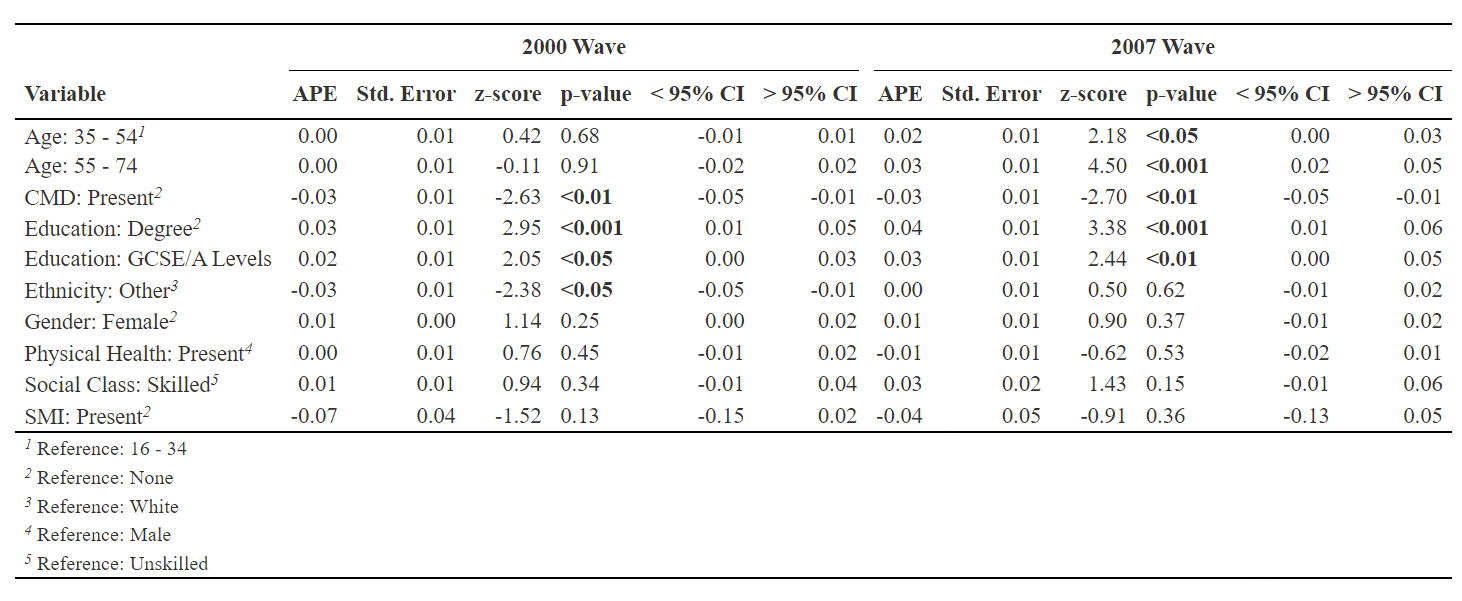
\includegraphics[width=460px,height=200px]{figure/apeemps} \caption[Average Partial Effects for for Employment Status]{Average Partial Effects for Employment Status in 2000 and 2007}\label{fig:apeemps}
\end{figure}
Average partial effects for employment status (Figure \ref{fig:apeemps}) can also be seen plotted in Figure \ref{fig:apeempsp}. Education, either gaining GCSE, A Levels or equivalent or a degree was the largest positive effect seen for being employed across both of the survey waves and were also statistically significant. Being within the skilled category within social class also had a positive effect on being employed across both survey years, although this was not significant. Being female also had a slight positive effect for being employed across both survey years, although not found to be statistically significant. Having a common mental health disorders present was also similar across survey years with a negative effect on being employed at 3\% less likely and both being statistically significant.

Differences in APE's across the years included age. Being aged 35 to 54 or 55 to 74 years old showed a small positive and statistically significant effect in the 2007 survey wave, but not for the 2000 wave. The UK economy experienced an overall growth between 2000 and 2007 which led to a decrease in unemployment rates, this could be one of the main factors that may have affected the job market and the employment prospects of people aged 35 to 54 and 55 to 74, leading to the difference in effect of age on employment status between the 2000 and 2007 survey waves. Additionally, government policies such as the introduction of the National Minimum wage in 1999, could have also played a role in the difference. Another difference was ethnicity. Being of non-white ethnicity was associated with a negative effect on likelihood of being employed in the 2000 survey wave but had a slight positive effect in the 2007 survey (-3\% vs 1\%). There were several policies and initiatives implemented by the UK government between 2000 and 2007 that aimed to increase employment opportunities and reduce discrimination against ethnic minorities that could explain this. These include the Race Relations (Amendment) Act 2000 which aimed to strengthen existing race discrimination laws and introduced new provisions to combat discrimination in the workplace. Also, the Race Equality Duty in 2006 required public bodies to eliminate discrimination and promote race equality in their policies and practices.

Another difference was the presence of severe mental illness, which was the largest negative effect associated with being employed in both survey years but improved in the 2007 wave (-7\% in the 2000 year and -5\% in the 2007 year). This on top of the large negative effect of severe mental illness on being economically activity in the first place. The National Service Framework for Mental Health (NSF) launched in 1999, aimed to improve the quality of care and services for people with mental health problems. The NSF set out specific standards and targets for mental health care, including improving access to treatments, reducing stigma and discrimination, and improving employment support for people with severe mental illness. This small improvement could also be explained by the introduction of the Disability Discrimination Act (DDA) 2005, aimed to tackle discrimination against people with disabilities, including people with severe mental illness. The act made it illegal for employers to discriminate against disabled employees, including those with severe mental illness, and required employers to make reasonable adjustments to the workplace to accommodate disabled workers.




\begin{figure}
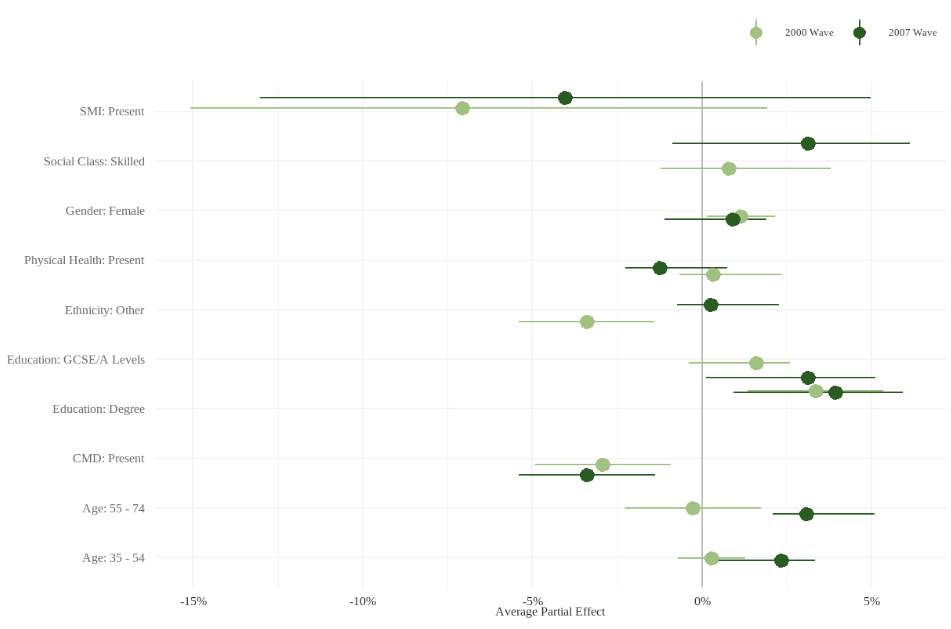
\includegraphics[width=450px,height=300px]{figure/apeempsp} \caption[Average Partial Effects Plot for Employment Status]{Average Partial Effects Plot for Employment Status in 2000 and 2007}\label{fig:apeempsp}
\end{figure}
\hypertarget{goodness-of-fit-for-employment-status}{%
\subsection{Goodness of Fit for Employment Status}\label{goodness-of-fit-for-employment-status}}

Figure \ref{fig:gofemps} shows the results of the diagnostic tests for the models applied to each of the survey waves with employment status as the outcome (being employed in comparison to unemployed). The McFadden's pseudo R2 statistic ranged from 0.030 for 2000 to 0.065 for 2007. The value of McFadden's pseudo R2 ranges from 0 to 1, with higher values indicating a better fit of the model to the data. A value of 0.030 and 0.065 would indicate that the models are weak and only explain a relatively small portion of the variation in the outcome variable. This may suggest that there are other factors that are not being considered by the model and that are influencing the outcome. It may also reflect the relatively small number of cases counted as `unemployed' and the fact that, for most, unemployment is a relatively short-lived state.




\begin{figure}
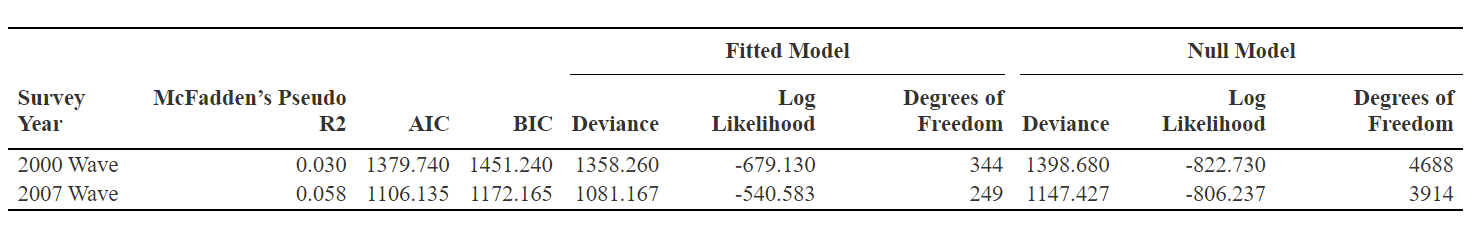
\includegraphics[width=460px,height=100px]{figure/gofemps} \caption[Goodness of Fit for Employment Status Models]{Goodness of Fit for Employment Status Models in 2000 and 2007}\label{fig:gofemps}
\end{figure}
\hypertarget{common-mental-health-disorders-and-economic-activity-1}{%
\section{Common Mental Health Disorders and Economic Activity}\label{common-mental-health-disorders-and-economic-activity-1}}

In this section, we return to the focus on economic activity (being active or not at the time of the survey being undertaken). In 6.2, we looked at the influence of having common mental health disorders or severe mental illness on activity. Here, we explore whether the use of health services or treatments for common mental health disorders might influence employment outcomes. The variables were having used any mental health services in the last year before being surveyed and undertaking any form of mental health treatment in that time, these being counselling, medication, or both. As previous research suggests that treatment use may indicate more severe levels of common mental health disorders, it is important to consider whether this may have a negative impact on economic activity. This effectively separates individuals with common mental health disorders into those who could be more ill and those who could be less ill.~The coefficient for common mental health disorders now reflects the effect for the default group which is now the least unwell i.e., those with no treatment or mental health service use. As in previous sections in this chapter, logistic regression models are applied to each year of data separately.

\hypertarget{model-results-for-common-mental-health-disorders-and-economic-activity}{%
\subsection{Model Results for Common Mental Health Disorders and Economic Activity}\label{model-results-for-common-mental-health-disorders-and-economic-activity}}

Table \ref{tab:results2-cmdmod} presents the results of logistic regression models examining the relationship between treatment use for common mental disorders and employment outcomes, using data from two survey waves in 2000 and 2007. The models control demographic, health, and educational factors. The adjusted odds ratios (AOR's) shown in the table indicate the effect of treatment use on the likelihood of being employed. As previous research suggests that treatment use may indicate more severe levels of common mental health disorders, it is important to note that the coefficients for common mental health disorders in the models reflect the effect of less severe (default) cases. The models include a total of 6,920 individuals from the 2000 survey wave and 5,736 individuals from the 2007 survey wave. Results show that several demographic and health factors, such as being female, having a physical health condition, and being aged 55-74, are negatively associated with employment with estimated effects very similar to the earlier model without treatment or service use. Having higher levels of education, such as GCSE's, A-level's, or a degree, also remains positively associated with employment.

The estimated effect for common mental health disorders (i.e., for those with common mental health disorders but not using services or receiving treatment) is substantially lower than before (for 2000, 0.69 compared with 0.51, and for 2007, 0.64 compared with 0.50). However, in both years, we see that even the least unwell in the common mental health disorders group still have greatly reduced probabilities of being economically active. For those using mental health services or receiving treatment, economic activity rates are lower still although it is worth noting that the effect of using counselling services alone not statistically significant in the 2007 survey wave.

\providecommand{\huxb}[2]{\arrayrulecolor[RGB]{#1}\global\arrayrulewidth=#2pt}
  \providecommand{\huxvb}[2]{\color[RGB]{#1}\vrule width #2pt}
  \providecommand{\huxtpad}[1]{\rule{0pt}{#1}}
  \providecommand{\huxbpad}[1]{\rule[-#1]{0pt}{#1}}
\begin{table}[h!]
\begin{centerbox}
\begin{threeparttable}
 \setlength{\tabcolsep}{0pt}
\begin{adjustbox}{width=1\textwidth}
\normalsize
\begin{tabular}{l l l l l l l l l}


\hhline{>{\arrayrulecolor[RGB]{0, 0, 0}\global\arrayrulewidth=0.4pt}->{\arrayrulecolor[RGB]{0, 0, 0}\global\arrayrulewidth=0.4pt}->{\arrayrulecolor[RGB]{0, 0, 0}\global\arrayrulewidth=0.4pt}->{\arrayrulecolor[RGB]{0, 0, 0}\global\arrayrulewidth=0.4pt}->{\arrayrulecolor[RGB]{0, 0, 0}\global\arrayrulewidth=0.4pt}->{\arrayrulecolor[RGB]{0, 0, 0}\global\arrayrulewidth=0.4pt}->{\arrayrulecolor[RGB]{0, 0, 0}\global\arrayrulewidth=0.4pt}->{\arrayrulecolor[RGB]{0, 0, 0}\global\arrayrulewidth=0.4pt}->{\arrayrulecolor[RGB]{0, 0, 0}\global\arrayrulewidth=0.4pt}-}
\arrayrulecolor{black}

\multicolumn{1}{!{\color[RGB]{0, 0, 0}\vrule width 0pt}l!{\color[RGB]{0, 0, 0}\vrule width 0pt}}{\rule{0pt}{1pt + 1em}\raggedright \hspace{0pt} \textbf{{\fontsize{14pt}{16.8pt}\selectfont 
}} \hspace{1pt}\rule[-1pt]{0pt}{1pt}} &
\multicolumn{4}{c!{\color[RGB]{0, 0, 0}\vrule width 0pt}}{\rule{0pt}{1pt + 1em}\centering \hspace{1pt} \textbf{{\fontsize{14pt}{16.8pt}\selectfont \textbf{2000 Wave}
}} \hspace{1pt}\rule[-1pt]{0pt}{1pt}} &
\multicolumn{4}{c!{\color[RGB]{0, 0, 0}\vrule width 0pt}}{\rule{0pt}{1pt + 1em}\centering \hspace{1pt} \textbf{{\fontsize{14pt}{16.8pt}\selectfont \textbf{2007 Wave}
}} \hspace{1pt}\rule[-1pt]{0pt}{1pt}} \tabularnewline[-0.5pt]


\hhline{}
\arrayrulecolor{black}

\multicolumn{1}{!{\color[RGB]{0, 0, 0}\vrule width 0pt}l!{\color[RGB]{0, 0, 0}\vrule width 0pt}}{\rule{0pt}{1pt + 1em}\raggedright \hspace{0pt} \textbf{{\fontsize{14pt}{16.8pt}\selectfont \textbf{Variable}
}} \hspace{1pt}\rule[-1pt]{0pt}{1pt}} &
\multicolumn{1}{c!{\color[RGB]{0, 0, 0}\vrule width 0pt}}{\rule{0pt}{1pt + 1em}\centering \hspace{1pt} \textbf{{\fontsize{14pt}{16.8pt}\selectfont \textbf{N}
}} \hspace{1pt}\rule[-1pt]{0pt}{1pt}} &
\multicolumn{1}{c!{\color[RGB]{0, 0, 0}\vrule width 0pt}}{\rule{0pt}{1pt + 1em}\centering \hspace{1pt} \textbf{{\fontsize{14pt}{16.8pt}\selectfont \textbf{OR}
}} \hspace{1pt}\rule[-1pt]{0pt}{1pt}} &
\multicolumn{1}{c!{\color[RGB]{0, 0, 0}\vrule width 0pt}}{\rule{0pt}{1pt + 1em}\centering \hspace{1pt} \textbf{{\fontsize{14pt}{16.8pt}\selectfont \textbf{95\% CI}
}} \hspace{1pt}\rule[-1pt]{0pt}{1pt}} &
\multicolumn{1}{c!{\color[RGB]{0, 0, 0}\vrule width 0pt}}{\rule{0pt}{1pt + 1em}\centering \hspace{1pt} \textbf{{\fontsize{14pt}{16.8pt}\selectfont \textbf{p-value}
}} \hspace{1pt}\rule[-1pt]{0pt}{1pt}} &
\multicolumn{1}{c!{\color[RGB]{0, 0, 0}\vrule width 0pt}}{\rule{0pt}{1pt + 1em}\centering \hspace{1pt} \textbf{{\fontsize{14pt}{16.8pt}\selectfont \textbf{N}
}} \hspace{1pt}\rule[-1pt]{0pt}{1pt}} &
\multicolumn{1}{c!{\color[RGB]{0, 0, 0}\vrule width 0pt}}{\rule{0pt}{1pt + 1em}\centering \hspace{1pt} \textbf{{\fontsize{14pt}{16.8pt}\selectfont \textbf{OR}
}} \hspace{1pt}\rule[-1pt]{0pt}{1pt}} &
\multicolumn{1}{c!{\color[RGB]{0, 0, 0}\vrule width 0pt}}{\rule{0pt}{1pt + 1em}\centering \hspace{1pt} \textbf{{\fontsize{14pt}{16.8pt}\selectfont \textbf{95\% CI}
}} \hspace{1pt}\rule[-1pt]{0pt}{1pt}} &
\multicolumn{1}{c!{\color[RGB]{0, 0, 0}\vrule width 0pt}}{\rule{0pt}{1pt + 1em}\centering \hspace{1pt} \textbf{{\fontsize{14pt}{16.8pt}\selectfont \textbf{p-value}
}} \hspace{0pt}\rule[-1pt]{0pt}{1pt}} \tabularnewline[-0.5pt]


\hhline{>{\arrayrulecolor[RGB]{0, 0, 0}\global\arrayrulewidth=0.4pt}->{\arrayrulecolor[RGB]{0, 0, 0}\global\arrayrulewidth=0.4pt}->{\arrayrulecolor[RGB]{0, 0, 0}\global\arrayrulewidth=0.4pt}->{\arrayrulecolor[RGB]{0, 0, 0}\global\arrayrulewidth=0.4pt}->{\arrayrulecolor[RGB]{0, 0, 0}\global\arrayrulewidth=0.4pt}->{\arrayrulecolor[RGB]{0, 0, 0}\global\arrayrulewidth=0.4pt}->{\arrayrulecolor[RGB]{0, 0, 0}\global\arrayrulewidth=0.4pt}->{\arrayrulecolor[RGB]{0, 0, 0}\global\arrayrulewidth=0.4pt}->{\arrayrulecolor[RGB]{0, 0, 0}\global\arrayrulewidth=0.4pt}-}
\arrayrulecolor{black}

\multicolumn{1}{!{\color[RGB]{0, 0, 0}\vrule width 0pt}l!{\color[RGB]{0, 0, 0}\vrule width 0pt}}{\rule{0pt}{1pt + 1em}\raggedright \hspace{0pt} \textbf{{\fontsize{14pt}{16.8pt}\selectfont Common Mental Health Disorder}} \hspace{1pt}\rule[-1pt]{0pt}{1pt}} &
\multicolumn{1}{c!{\color[RGB]{0, 0, 0}\vrule width 0pt}}{\rule{0pt}{1pt + 1em}\centering \hspace{1pt} {\fontsize{14pt}{16.8pt}\selectfont 6,920} \hspace{1pt}\rule[-1pt]{0pt}{1pt}} &
\multicolumn{1}{c!{\color[RGB]{0, 0, 0}\vrule width 0pt}}{\rule{0pt}{1pt + 1em}\centering \hspace{1pt} {\fontsize{14pt}{16.8pt}\selectfont } \hspace{1pt}\rule[-1pt]{0pt}{1pt}} &
\multicolumn{1}{c!{\color[RGB]{0, 0, 0}\vrule width 0pt}}{\rule{0pt}{1pt + 1em}\centering \hspace{1pt} {\fontsize{14pt}{16.8pt}\selectfont } \hspace{1pt}\rule[-1pt]{0pt}{1pt}} &
\multicolumn{1}{c!{\color[RGB]{0, 0, 0}\vrule width 0pt}}{\rule{0pt}{1pt + 1em}\centering \hspace{1pt} {\fontsize{14pt}{16.8pt}\selectfont } \hspace{1pt}\rule[-1pt]{0pt}{1pt}} &
\multicolumn{1}{c!{\color[RGB]{0, 0, 0}\vrule width 0pt}}{\rule{0pt}{1pt + 1em}\centering \hspace{1pt} {\fontsize{14pt}{16.8pt}\selectfont 5,736} \hspace{1pt}\rule[-1pt]{0pt}{1pt}} &
\multicolumn{1}{c!{\color[RGB]{0, 0, 0}\vrule width 0pt}}{\rule{0pt}{1pt + 1em}\centering \hspace{1pt} {\fontsize{14pt}{16.8pt}\selectfont } \hspace{1pt}\rule[-1pt]{0pt}{1pt}} &
\multicolumn{1}{c!{\color[RGB]{0, 0, 0}\vrule width 0pt}}{\rule{0pt}{1pt + 1em}\centering \hspace{1pt} {\fontsize{14pt}{16.8pt}\selectfont } \hspace{1pt}\rule[-1pt]{0pt}{1pt}} &
\multicolumn{1}{c!{\color[RGB]{0, 0, 0}\vrule width 0pt}}{\rule{0pt}{1pt + 1em}\centering \hspace{1pt} {\fontsize{14pt}{16.8pt}\selectfont } \hspace{0pt}\rule[-1pt]{0pt}{1pt}} \tabularnewline[-0.5pt]


\hhline{}
\arrayrulecolor{black}

\multicolumn{1}{!{\color[RGB]{0, 0, 0}\vrule width 0pt}l!{\color[RGB]{0, 0, 0}\vrule width 0pt}}{\rule{0pt}{1pt + 1em}\raggedright \hspace{0pt} {\fontsize{14pt}{16.8pt}\selectfont None} \hspace{1pt}\rule[-1pt]{0pt}{1pt}} &
\multicolumn{1}{c!{\color[RGB]{0, 0, 0}\vrule width 0pt}}{\rule{0pt}{1pt + 1em}\centering \hspace{1pt} {\fontsize{14pt}{16.8pt}\selectfont } \hspace{1pt}\rule[-1pt]{0pt}{1pt}} &
\multicolumn{1}{c!{\color[RGB]{0, 0, 0}\vrule width 0pt}}{\rule{0pt}{1pt + 1em}\centering \hspace{1pt} {\fontsize{14pt}{16.8pt}\selectfont —} \hspace{1pt}\rule[-1pt]{0pt}{1pt}} &
\multicolumn{1}{c!{\color[RGB]{0, 0, 0}\vrule width 0pt}}{\rule{0pt}{1pt + 1em}\centering \hspace{1pt} {\fontsize{14pt}{16.8pt}\selectfont —} \hspace{1pt}\rule[-1pt]{0pt}{1pt}} &
\multicolumn{1}{c!{\color[RGB]{0, 0, 0}\vrule width 0pt}}{\rule{0pt}{1pt + 1em}\centering \hspace{1pt} {\fontsize{14pt}{16.8pt}\selectfont } \hspace{1pt}\rule[-1pt]{0pt}{1pt}} &
\multicolumn{1}{c!{\color[RGB]{0, 0, 0}\vrule width 0pt}}{\rule{0pt}{1pt + 1em}\centering \hspace{1pt} {\fontsize{14pt}{16.8pt}\selectfont } \hspace{1pt}\rule[-1pt]{0pt}{1pt}} &
\multicolumn{1}{c!{\color[RGB]{0, 0, 0}\vrule width 0pt}}{\rule{0pt}{1pt + 1em}\centering \hspace{1pt} {\fontsize{14pt}{16.8pt}\selectfont —} \hspace{1pt}\rule[-1pt]{0pt}{1pt}} &
\multicolumn{1}{c!{\color[RGB]{0, 0, 0}\vrule width 0pt}}{\rule{0pt}{1pt + 1em}\centering \hspace{1pt} {\fontsize{14pt}{16.8pt}\selectfont —} \hspace{1pt}\rule[-1pt]{0pt}{1pt}} &
\multicolumn{1}{c!{\color[RGB]{0, 0, 0}\vrule width 0pt}}{\rule{0pt}{1pt + 1em}\centering \hspace{1pt} {\fontsize{14pt}{16.8pt}\selectfont } \hspace{0pt}\rule[-1pt]{0pt}{1pt}} \tabularnewline[-0.5pt]


\hhline{}
\arrayrulecolor{black}

\multicolumn{1}{!{\color[RGB]{0, 0, 0}\vrule width 0pt}l!{\color[RGB]{0, 0, 0}\vrule width 0pt}}{\rule{0pt}{1pt + 1em}\raggedright \hspace{0pt} {\fontsize{14pt}{16.8pt}\selectfont Present} \hspace{1pt}\rule[-1pt]{0pt}{1pt}} &
\multicolumn{1}{c!{\color[RGB]{0, 0, 0}\vrule width 0pt}}{\rule{0pt}{1pt + 1em}\centering \hspace{1pt} {\fontsize{14pt}{16.8pt}\selectfont } \hspace{1pt}\rule[-1pt]{0pt}{1pt}} &
\multicolumn{1}{c!{\color[RGB]{0, 0, 0}\vrule width 0pt}}{\rule{0pt}{1pt + 1em}\centering \hspace{1pt} {\fontsize{14pt}{16.8pt}\selectfont 0.69} \hspace{1pt}\rule[-1pt]{0pt}{1pt}} &
\multicolumn{1}{c!{\color[RGB]{0, 0, 0}\vrule width 0pt}}{\rule{0pt}{1pt + 1em}\centering \hspace{1pt} {\fontsize{14pt}{16.8pt}\selectfont 0.57, 0.85} \hspace{1pt}\rule[-1pt]{0pt}{1pt}} &
\multicolumn{1}{c!{\color[RGB]{0, 0, 0}\vrule width 0pt}}{\rule{0pt}{1pt + 1em}\centering \hspace{1pt} \textbf{{\fontsize{14pt}{16.8pt}\selectfont $<$0.001}} \hspace{1pt}\rule[-1pt]{0pt}{1pt}} &
\multicolumn{1}{c!{\color[RGB]{0, 0, 0}\vrule width 0pt}}{\rule{0pt}{1pt + 1em}\centering \hspace{1pt} {\fontsize{14pt}{16.8pt}\selectfont } \hspace{1pt}\rule[-1pt]{0pt}{1pt}} &
\multicolumn{1}{c!{\color[RGB]{0, 0, 0}\vrule width 0pt}}{\rule{0pt}{1pt + 1em}\centering \hspace{1pt} {\fontsize{14pt}{16.8pt}\selectfont 0.64} \hspace{1pt}\rule[-1pt]{0pt}{1pt}} &
\multicolumn{1}{c!{\color[RGB]{0, 0, 0}\vrule width 0pt}}{\rule{0pt}{1pt + 1em}\centering \hspace{1pt} {\fontsize{14pt}{16.8pt}\selectfont 0.52, 0.79} \hspace{1pt}\rule[-1pt]{0pt}{1pt}} &
\multicolumn{1}{c!{\color[RGB]{0, 0, 0}\vrule width 0pt}}{\rule{0pt}{1pt + 1em}\centering \hspace{1pt} \textbf{{\fontsize{14pt}{16.8pt}\selectfont $<$0.001}} \hspace{0pt}\rule[-1pt]{0pt}{1pt}} \tabularnewline[-0.5pt]


\hhline{}
\arrayrulecolor{black}

\multicolumn{1}{!{\color[RGB]{0, 0, 0}\vrule width 0pt}l!{\color[RGB]{0, 0, 0}\vrule width 0pt}}{\rule{0pt}{1pt + 1em}\raggedright \hspace{0pt} \textbf{{\fontsize{14pt}{16.8pt}\selectfont gender}} \hspace{1pt}\rule[-1pt]{0pt}{1pt}} &
\multicolumn{1}{c!{\color[RGB]{0, 0, 0}\vrule width 0pt}}{\rule{0pt}{1pt + 1em}\centering \hspace{1pt} {\fontsize{14pt}{16.8pt}\selectfont 6,920} \hspace{1pt}\rule[-1pt]{0pt}{1pt}} &
\multicolumn{1}{c!{\color[RGB]{0, 0, 0}\vrule width 0pt}}{\rule{0pt}{1pt + 1em}\centering \hspace{1pt} {\fontsize{14pt}{16.8pt}\selectfont } \hspace{1pt}\rule[-1pt]{0pt}{1pt}} &
\multicolumn{1}{c!{\color[RGB]{0, 0, 0}\vrule width 0pt}}{\rule{0pt}{1pt + 1em}\centering \hspace{1pt} {\fontsize{14pt}{16.8pt}\selectfont } \hspace{1pt}\rule[-1pt]{0pt}{1pt}} &
\multicolumn{1}{c!{\color[RGB]{0, 0, 0}\vrule width 0pt}}{\rule{0pt}{1pt + 1em}\centering \hspace{1pt} {\fontsize{14pt}{16.8pt}\selectfont } \hspace{1pt}\rule[-1pt]{0pt}{1pt}} &
\multicolumn{1}{c!{\color[RGB]{0, 0, 0}\vrule width 0pt}}{\rule{0pt}{1pt + 1em}\centering \hspace{1pt} {\fontsize{14pt}{16.8pt}\selectfont 5,736} \hspace{1pt}\rule[-1pt]{0pt}{1pt}} &
\multicolumn{1}{c!{\color[RGB]{0, 0, 0}\vrule width 0pt}}{\rule{0pt}{1pt + 1em}\centering \hspace{1pt} {\fontsize{14pt}{16.8pt}\selectfont } \hspace{1pt}\rule[-1pt]{0pt}{1pt}} &
\multicolumn{1}{c!{\color[RGB]{0, 0, 0}\vrule width 0pt}}{\rule{0pt}{1pt + 1em}\centering \hspace{1pt} {\fontsize{14pt}{16.8pt}\selectfont } \hspace{1pt}\rule[-1pt]{0pt}{1pt}} &
\multicolumn{1}{c!{\color[RGB]{0, 0, 0}\vrule width 0pt}}{\rule{0pt}{1pt + 1em}\centering \hspace{1pt} {\fontsize{14pt}{16.8pt}\selectfont } \hspace{0pt}\rule[-1pt]{0pt}{1pt}} \tabularnewline[-0.5pt]


\hhline{}
\arrayrulecolor{black}

\multicolumn{1}{!{\color[RGB]{0, 0, 0}\vrule width 0pt}l!{\color[RGB]{0, 0, 0}\vrule width 0pt}}{\rule{0pt}{1pt + 1em}\raggedright \hspace{0pt} {\fontsize{14pt}{16.8pt}\selectfont Male} \hspace{1pt}\rule[-1pt]{0pt}{1pt}} &
\multicolumn{1}{c!{\color[RGB]{0, 0, 0}\vrule width 0pt}}{\rule{0pt}{1pt + 1em}\centering \hspace{1pt} {\fontsize{14pt}{16.8pt}\selectfont } \hspace{1pt}\rule[-1pt]{0pt}{1pt}} &
\multicolumn{1}{c!{\color[RGB]{0, 0, 0}\vrule width 0pt}}{\rule{0pt}{1pt + 1em}\centering \hspace{1pt} {\fontsize{14pt}{16.8pt}\selectfont —} \hspace{1pt}\rule[-1pt]{0pt}{1pt}} &
\multicolumn{1}{c!{\color[RGB]{0, 0, 0}\vrule width 0pt}}{\rule{0pt}{1pt + 1em}\centering \hspace{1pt} {\fontsize{14pt}{16.8pt}\selectfont —} \hspace{1pt}\rule[-1pt]{0pt}{1pt}} &
\multicolumn{1}{c!{\color[RGB]{0, 0, 0}\vrule width 0pt}}{\rule{0pt}{1pt + 1em}\centering \hspace{1pt} {\fontsize{14pt}{16.8pt}\selectfont } \hspace{1pt}\rule[-1pt]{0pt}{1pt}} &
\multicolumn{1}{c!{\color[RGB]{0, 0, 0}\vrule width 0pt}}{\rule{0pt}{1pt + 1em}\centering \hspace{1pt} {\fontsize{14pt}{16.8pt}\selectfont } \hspace{1pt}\rule[-1pt]{0pt}{1pt}} &
\multicolumn{1}{c!{\color[RGB]{0, 0, 0}\vrule width 0pt}}{\rule{0pt}{1pt + 1em}\centering \hspace{1pt} {\fontsize{14pt}{16.8pt}\selectfont —} \hspace{1pt}\rule[-1pt]{0pt}{1pt}} &
\multicolumn{1}{c!{\color[RGB]{0, 0, 0}\vrule width 0pt}}{\rule{0pt}{1pt + 1em}\centering \hspace{1pt} {\fontsize{14pt}{16.8pt}\selectfont —} \hspace{1pt}\rule[-1pt]{0pt}{1pt}} &
\multicolumn{1}{c!{\color[RGB]{0, 0, 0}\vrule width 0pt}}{\rule{0pt}{1pt + 1em}\centering \hspace{1pt} {\fontsize{14pt}{16.8pt}\selectfont } \hspace{0pt}\rule[-1pt]{0pt}{1pt}} \tabularnewline[-0.5pt]


\hhline{}
\arrayrulecolor{black}

\multicolumn{1}{!{\color[RGB]{0, 0, 0}\vrule width 0pt}l!{\color[RGB]{0, 0, 0}\vrule width 0pt}}{\rule{0pt}{1pt + 1em}\raggedright \hspace{0pt} {\fontsize{14pt}{16.8pt}\selectfont Female} \hspace{1pt}\rule[-1pt]{0pt}{1pt}} &
\multicolumn{1}{c!{\color[RGB]{0, 0, 0}\vrule width 0pt}}{\rule{0pt}{1pt + 1em}\centering \hspace{1pt} {\fontsize{14pt}{16.8pt}\selectfont } \hspace{1pt}\rule[-1pt]{0pt}{1pt}} &
\multicolumn{1}{c!{\color[RGB]{0, 0, 0}\vrule width 0pt}}{\rule{0pt}{1pt + 1em}\centering \hspace{1pt} {\fontsize{14pt}{16.8pt}\selectfont 0.41} \hspace{1pt}\rule[-1pt]{0pt}{1pt}} &
\multicolumn{1}{c!{\color[RGB]{0, 0, 0}\vrule width 0pt}}{\rule{0pt}{1pt + 1em}\centering \hspace{1pt} {\fontsize{14pt}{16.8pt}\selectfont 0.35, 0.47} \hspace{1pt}\rule[-1pt]{0pt}{1pt}} &
\multicolumn{1}{c!{\color[RGB]{0, 0, 0}\vrule width 0pt}}{\rule{0pt}{1pt + 1em}\centering \hspace{1pt} \textbf{{\fontsize{14pt}{16.8pt}\selectfont $<$0.001}} \hspace{1pt}\rule[-1pt]{0pt}{1pt}} &
\multicolumn{1}{c!{\color[RGB]{0, 0, 0}\vrule width 0pt}}{\rule{0pt}{1pt + 1em}\centering \hspace{1pt} {\fontsize{14pt}{16.8pt}\selectfont } \hspace{1pt}\rule[-1pt]{0pt}{1pt}} &
\multicolumn{1}{c!{\color[RGB]{0, 0, 0}\vrule width 0pt}}{\rule{0pt}{1pt + 1em}\centering \hspace{1pt} {\fontsize{14pt}{16.8pt}\selectfont 0.47} \hspace{1pt}\rule[-1pt]{0pt}{1pt}} &
\multicolumn{1}{c!{\color[RGB]{0, 0, 0}\vrule width 0pt}}{\rule{0pt}{1pt + 1em}\centering \hspace{1pt} {\fontsize{14pt}{16.8pt}\selectfont 0.40, 0.54} \hspace{1pt}\rule[-1pt]{0pt}{1pt}} &
\multicolumn{1}{c!{\color[RGB]{0, 0, 0}\vrule width 0pt}}{\rule{0pt}{1pt + 1em}\centering \hspace{1pt} \textbf{{\fontsize{14pt}{16.8pt}\selectfont $<$0.001}} \hspace{0pt}\rule[-1pt]{0pt}{1pt}} \tabularnewline[-0.5pt]


\hhline{}
\arrayrulecolor{black}

\multicolumn{1}{!{\color[RGB]{0, 0, 0}\vrule width 0pt}l!{\color[RGB]{0, 0, 0}\vrule width 0pt}}{\rule{0pt}{1pt + 1em}\raggedright \hspace{0pt} \textbf{{\fontsize{14pt}{16.8pt}\selectfont Age Band}} \hspace{1pt}\rule[-1pt]{0pt}{1pt}} &
\multicolumn{1}{c!{\color[RGB]{0, 0, 0}\vrule width 0pt}}{\rule{0pt}{1pt + 1em}\centering \hspace{1pt} {\fontsize{14pt}{16.8pt}\selectfont 6,920} \hspace{1pt}\rule[-1pt]{0pt}{1pt}} &
\multicolumn{1}{c!{\color[RGB]{0, 0, 0}\vrule width 0pt}}{\rule{0pt}{1pt + 1em}\centering \hspace{1pt} {\fontsize{14pt}{16.8pt}\selectfont } \hspace{1pt}\rule[-1pt]{0pt}{1pt}} &
\multicolumn{1}{c!{\color[RGB]{0, 0, 0}\vrule width 0pt}}{\rule{0pt}{1pt + 1em}\centering \hspace{1pt} {\fontsize{14pt}{16.8pt}\selectfont } \hspace{1pt}\rule[-1pt]{0pt}{1pt}} &
\multicolumn{1}{c!{\color[RGB]{0, 0, 0}\vrule width 0pt}}{\rule{0pt}{1pt + 1em}\centering \hspace{1pt} {\fontsize{14pt}{16.8pt}\selectfont } \hspace{1pt}\rule[-1pt]{0pt}{1pt}} &
\multicolumn{1}{c!{\color[RGB]{0, 0, 0}\vrule width 0pt}}{\rule{0pt}{1pt + 1em}\centering \hspace{1pt} {\fontsize{14pt}{16.8pt}\selectfont 5,736} \hspace{1pt}\rule[-1pt]{0pt}{1pt}} &
\multicolumn{1}{c!{\color[RGB]{0, 0, 0}\vrule width 0pt}}{\rule{0pt}{1pt + 1em}\centering \hspace{1pt} {\fontsize{14pt}{16.8pt}\selectfont } \hspace{1pt}\rule[-1pt]{0pt}{1pt}} &
\multicolumn{1}{c!{\color[RGB]{0, 0, 0}\vrule width 0pt}}{\rule{0pt}{1pt + 1em}\centering \hspace{1pt} {\fontsize{14pt}{16.8pt}\selectfont } \hspace{1pt}\rule[-1pt]{0pt}{1pt}} &
\multicolumn{1}{c!{\color[RGB]{0, 0, 0}\vrule width 0pt}}{\rule{0pt}{1pt + 1em}\centering \hspace{1pt} {\fontsize{14pt}{16.8pt}\selectfont } \hspace{0pt}\rule[-1pt]{0pt}{1pt}} \tabularnewline[-0.5pt]


\hhline{}
\arrayrulecolor{black}

\multicolumn{1}{!{\color[RGB]{0, 0, 0}\vrule width 0pt}l!{\color[RGB]{0, 0, 0}\vrule width 0pt}}{\rule{0pt}{1pt + 1em}\raggedright \hspace{0pt} {\fontsize{14pt}{16.8pt}\selectfont 16 - 34} \hspace{1pt}\rule[-1pt]{0pt}{1pt}} &
\multicolumn{1}{c!{\color[RGB]{0, 0, 0}\vrule width 0pt}}{\rule{0pt}{1pt + 1em}\centering \hspace{1pt} {\fontsize{14pt}{16.8pt}\selectfont } \hspace{1pt}\rule[-1pt]{0pt}{1pt}} &
\multicolumn{1}{c!{\color[RGB]{0, 0, 0}\vrule width 0pt}}{\rule{0pt}{1pt + 1em}\centering \hspace{1pt} {\fontsize{14pt}{16.8pt}\selectfont —} \hspace{1pt}\rule[-1pt]{0pt}{1pt}} &
\multicolumn{1}{c!{\color[RGB]{0, 0, 0}\vrule width 0pt}}{\rule{0pt}{1pt + 1em}\centering \hspace{1pt} {\fontsize{14pt}{16.8pt}\selectfont —} \hspace{1pt}\rule[-1pt]{0pt}{1pt}} &
\multicolumn{1}{c!{\color[RGB]{0, 0, 0}\vrule width 0pt}}{\rule{0pt}{1pt + 1em}\centering \hspace{1pt} {\fontsize{14pt}{16.8pt}\selectfont } \hspace{1pt}\rule[-1pt]{0pt}{1pt}} &
\multicolumn{1}{c!{\color[RGB]{0, 0, 0}\vrule width 0pt}}{\rule{0pt}{1pt + 1em}\centering \hspace{1pt} {\fontsize{14pt}{16.8pt}\selectfont } \hspace{1pt}\rule[-1pt]{0pt}{1pt}} &
\multicolumn{1}{c!{\color[RGB]{0, 0, 0}\vrule width 0pt}}{\rule{0pt}{1pt + 1em}\centering \hspace{1pt} {\fontsize{14pt}{16.8pt}\selectfont —} \hspace{1pt}\rule[-1pt]{0pt}{1pt}} &
\multicolumn{1}{c!{\color[RGB]{0, 0, 0}\vrule width 0pt}}{\rule{0pt}{1pt + 1em}\centering \hspace{1pt} {\fontsize{14pt}{16.8pt}\selectfont —} \hspace{1pt}\rule[-1pt]{0pt}{1pt}} &
\multicolumn{1}{c!{\color[RGB]{0, 0, 0}\vrule width 0pt}}{\rule{0pt}{1pt + 1em}\centering \hspace{1pt} {\fontsize{14pt}{16.8pt}\selectfont } \hspace{0pt}\rule[-1pt]{0pt}{1pt}} \tabularnewline[-0.5pt]


\hhline{}
\arrayrulecolor{black}

\multicolumn{1}{!{\color[RGB]{0, 0, 0}\vrule width 0pt}l!{\color[RGB]{0, 0, 0}\vrule width 0pt}}{\rule{0pt}{1pt + 1em}\raggedright \hspace{0pt} {\fontsize{14pt}{16.8pt}\selectfont 35 - 54} \hspace{1pt}\rule[-1pt]{0pt}{1pt}} &
\multicolumn{1}{c!{\color[RGB]{0, 0, 0}\vrule width 0pt}}{\rule{0pt}{1pt + 1em}\centering \hspace{1pt} {\fontsize{14pt}{16.8pt}\selectfont } \hspace{1pt}\rule[-1pt]{0pt}{1pt}} &
\multicolumn{1}{c!{\color[RGB]{0, 0, 0}\vrule width 0pt}}{\rule{0pt}{1pt + 1em}\centering \hspace{1pt} {\fontsize{14pt}{16.8pt}\selectfont 0.92} \hspace{1pt}\rule[-1pt]{0pt}{1pt}} &
\multicolumn{1}{c!{\color[RGB]{0, 0, 0}\vrule width 0pt}}{\rule{0pt}{1pt + 1em}\centering \hspace{1pt} {\fontsize{14pt}{16.8pt}\selectfont 0.78, 1.09} \hspace{1pt}\rule[-1pt]{0pt}{1pt}} &
\multicolumn{1}{c!{\color[RGB]{0, 0, 0}\vrule width 0pt}}{\rule{0pt}{1pt + 1em}\centering \hspace{1pt} {\fontsize{14pt}{16.8pt}\selectfont 0.35} \hspace{1pt}\rule[-1pt]{0pt}{1pt}} &
\multicolumn{1}{c!{\color[RGB]{0, 0, 0}\vrule width 0pt}}{\rule{0pt}{1pt + 1em}\centering \hspace{1pt} {\fontsize{14pt}{16.8pt}\selectfont } \hspace{1pt}\rule[-1pt]{0pt}{1pt}} &
\multicolumn{1}{c!{\color[RGB]{0, 0, 0}\vrule width 0pt}}{\rule{0pt}{1pt + 1em}\centering \hspace{1pt} {\fontsize{14pt}{16.8pt}\selectfont 1.10} \hspace{1pt}\rule[-1pt]{0pt}{1pt}} &
\multicolumn{1}{c!{\color[RGB]{0, 0, 0}\vrule width 0pt}}{\rule{0pt}{1pt + 1em}\centering \hspace{1pt} {\fontsize{14pt}{16.8pt}\selectfont 0.88, 1.39} \hspace{1pt}\rule[-1pt]{0pt}{1pt}} &
\multicolumn{1}{c!{\color[RGB]{0, 0, 0}\vrule width 0pt}}{\rule{0pt}{1pt + 1em}\centering \hspace{1pt} {\fontsize{14pt}{16.8pt}\selectfont 0.40} \hspace{0pt}\rule[-1pt]{0pt}{1pt}} \tabularnewline[-0.5pt]


\hhline{}
\arrayrulecolor{black}

\multicolumn{1}{!{\color[RGB]{0, 0, 0}\vrule width 0pt}l!{\color[RGB]{0, 0, 0}\vrule width 0pt}}{\rule{0pt}{1pt + 1em}\raggedright \hspace{0pt} {\fontsize{14pt}{16.8pt}\selectfont 55 - 74} \hspace{1pt}\rule[-1pt]{0pt}{1pt}} &
\multicolumn{1}{c!{\color[RGB]{0, 0, 0}\vrule width 0pt}}{\rule{0pt}{1pt + 1em}\centering \hspace{1pt} {\fontsize{14pt}{16.8pt}\selectfont } \hspace{1pt}\rule[-1pt]{0pt}{1pt}} &
\multicolumn{1}{c!{\color[RGB]{0, 0, 0}\vrule width 0pt}}{\rule{0pt}{1pt + 1em}\centering \hspace{1pt} {\fontsize{14pt}{16.8pt}\selectfont 0.08} \hspace{1pt}\rule[-1pt]{0pt}{1pt}} &
\multicolumn{1}{c!{\color[RGB]{0, 0, 0}\vrule width 0pt}}{\rule{0pt}{1pt + 1em}\centering \hspace{1pt} {\fontsize{14pt}{16.8pt}\selectfont 0.07, 0.10} \hspace{1pt}\rule[-1pt]{0pt}{1pt}} &
\multicolumn{1}{c!{\color[RGB]{0, 0, 0}\vrule width 0pt}}{\rule{0pt}{1pt + 1em}\centering \hspace{1pt} \textbf{{\fontsize{14pt}{16.8pt}\selectfont $<$0.001}} \hspace{1pt}\rule[-1pt]{0pt}{1pt}} &
\multicolumn{1}{c!{\color[RGB]{0, 0, 0}\vrule width 0pt}}{\rule{0pt}{1pt + 1em}\centering \hspace{1pt} {\fontsize{14pt}{16.8pt}\selectfont } \hspace{1pt}\rule[-1pt]{0pt}{1pt}} &
\multicolumn{1}{c!{\color[RGB]{0, 0, 0}\vrule width 0pt}}{\rule{0pt}{1pt + 1em}\centering \hspace{1pt} {\fontsize{14pt}{16.8pt}\selectfont 0.13} \hspace{1pt}\rule[-1pt]{0pt}{1pt}} &
\multicolumn{1}{c!{\color[RGB]{0, 0, 0}\vrule width 0pt}}{\rule{0pt}{1pt + 1em}\centering \hspace{1pt} {\fontsize{14pt}{16.8pt}\selectfont 0.10, 0.16} \hspace{1pt}\rule[-1pt]{0pt}{1pt}} &
\multicolumn{1}{c!{\color[RGB]{0, 0, 0}\vrule width 0pt}}{\rule{0pt}{1pt + 1em}\centering \hspace{1pt} \textbf{{\fontsize{14pt}{16.8pt}\selectfont $<$0.001}} \hspace{0pt}\rule[-1pt]{0pt}{1pt}} \tabularnewline[-0.5pt]


\hhline{}
\arrayrulecolor{black}

\multicolumn{1}{!{\color[RGB]{0, 0, 0}\vrule width 0pt}l!{\color[RGB]{0, 0, 0}\vrule width 0pt}}{\rule{0pt}{1pt + 1em}\raggedright \hspace{0pt} \textbf{{\fontsize{14pt}{16.8pt}\selectfont Ethnicity}} \hspace{1pt}\rule[-1pt]{0pt}{1pt}} &
\multicolumn{1}{c!{\color[RGB]{0, 0, 0}\vrule width 0pt}}{\rule{0pt}{1pt + 1em}\centering \hspace{1pt} {\fontsize{14pt}{16.8pt}\selectfont 6,920} \hspace{1pt}\rule[-1pt]{0pt}{1pt}} &
\multicolumn{1}{c!{\color[RGB]{0, 0, 0}\vrule width 0pt}}{\rule{0pt}{1pt + 1em}\centering \hspace{1pt} {\fontsize{14pt}{16.8pt}\selectfont } \hspace{1pt}\rule[-1pt]{0pt}{1pt}} &
\multicolumn{1}{c!{\color[RGB]{0, 0, 0}\vrule width 0pt}}{\rule{0pt}{1pt + 1em}\centering \hspace{1pt} {\fontsize{14pt}{16.8pt}\selectfont } \hspace{1pt}\rule[-1pt]{0pt}{1pt}} &
\multicolumn{1}{c!{\color[RGB]{0, 0, 0}\vrule width 0pt}}{\rule{0pt}{1pt + 1em}\centering \hspace{1pt} {\fontsize{14pt}{16.8pt}\selectfont } \hspace{1pt}\rule[-1pt]{0pt}{1pt}} &
\multicolumn{1}{c!{\color[RGB]{0, 0, 0}\vrule width 0pt}}{\rule{0pt}{1pt + 1em}\centering \hspace{1pt} {\fontsize{14pt}{16.8pt}\selectfont 5,736} \hspace{1pt}\rule[-1pt]{0pt}{1pt}} &
\multicolumn{1}{c!{\color[RGB]{0, 0, 0}\vrule width 0pt}}{\rule{0pt}{1pt + 1em}\centering \hspace{1pt} {\fontsize{14pt}{16.8pt}\selectfont } \hspace{1pt}\rule[-1pt]{0pt}{1pt}} &
\multicolumn{1}{c!{\color[RGB]{0, 0, 0}\vrule width 0pt}}{\rule{0pt}{1pt + 1em}\centering \hspace{1pt} {\fontsize{14pt}{16.8pt}\selectfont } \hspace{1pt}\rule[-1pt]{0pt}{1pt}} &
\multicolumn{1}{c!{\color[RGB]{0, 0, 0}\vrule width 0pt}}{\rule{0pt}{1pt + 1em}\centering \hspace{1pt} {\fontsize{14pt}{16.8pt}\selectfont } \hspace{0pt}\rule[-1pt]{0pt}{1pt}} \tabularnewline[-0.5pt]


\hhline{}
\arrayrulecolor{black}

\multicolumn{1}{!{\color[RGB]{0, 0, 0}\vrule width 0pt}l!{\color[RGB]{0, 0, 0}\vrule width 0pt}}{\rule{0pt}{1pt + 1em}\raggedright \hspace{0pt} {\fontsize{14pt}{16.8pt}\selectfont White} \hspace{1pt}\rule[-1pt]{0pt}{1pt}} &
\multicolumn{1}{c!{\color[RGB]{0, 0, 0}\vrule width 0pt}}{\rule{0pt}{1pt + 1em}\centering \hspace{1pt} {\fontsize{14pt}{16.8pt}\selectfont } \hspace{1pt}\rule[-1pt]{0pt}{1pt}} &
\multicolumn{1}{c!{\color[RGB]{0, 0, 0}\vrule width 0pt}}{\rule{0pt}{1pt + 1em}\centering \hspace{1pt} {\fontsize{14pt}{16.8pt}\selectfont —} \hspace{1pt}\rule[-1pt]{0pt}{1pt}} &
\multicolumn{1}{c!{\color[RGB]{0, 0, 0}\vrule width 0pt}}{\rule{0pt}{1pt + 1em}\centering \hspace{1pt} {\fontsize{14pt}{16.8pt}\selectfont —} \hspace{1pt}\rule[-1pt]{0pt}{1pt}} &
\multicolumn{1}{c!{\color[RGB]{0, 0, 0}\vrule width 0pt}}{\rule{0pt}{1pt + 1em}\centering \hspace{1pt} {\fontsize{14pt}{16.8pt}\selectfont } \hspace{1pt}\rule[-1pt]{0pt}{1pt}} &
\multicolumn{1}{c!{\color[RGB]{0, 0, 0}\vrule width 0pt}}{\rule{0pt}{1pt + 1em}\centering \hspace{1pt} {\fontsize{14pt}{16.8pt}\selectfont } \hspace{1pt}\rule[-1pt]{0pt}{1pt}} &
\multicolumn{1}{c!{\color[RGB]{0, 0, 0}\vrule width 0pt}}{\rule{0pt}{1pt + 1em}\centering \hspace{1pt} {\fontsize{14pt}{16.8pt}\selectfont —} \hspace{1pt}\rule[-1pt]{0pt}{1pt}} &
\multicolumn{1}{c!{\color[RGB]{0, 0, 0}\vrule width 0pt}}{\rule{0pt}{1pt + 1em}\centering \hspace{1pt} {\fontsize{14pt}{16.8pt}\selectfont —} \hspace{1pt}\rule[-1pt]{0pt}{1pt}} &
\multicolumn{1}{c!{\color[RGB]{0, 0, 0}\vrule width 0pt}}{\rule{0pt}{1pt + 1em}\centering \hspace{1pt} {\fontsize{14pt}{16.8pt}\selectfont } \hspace{0pt}\rule[-1pt]{0pt}{1pt}} \tabularnewline[-0.5pt]


\hhline{}
\arrayrulecolor{black}

\multicolumn{1}{!{\color[RGB]{0, 0, 0}\vrule width 0pt}l!{\color[RGB]{0, 0, 0}\vrule width 0pt}}{\rule{0pt}{1pt + 1em}\raggedright \hspace{0pt} {\fontsize{14pt}{16.8pt}\selectfont Other} \hspace{1pt}\rule[-1pt]{0pt}{1pt}} &
\multicolumn{1}{c!{\color[RGB]{0, 0, 0}\vrule width 0pt}}{\rule{0pt}{1pt + 1em}\centering \hspace{1pt} {\fontsize{14pt}{16.8pt}\selectfont } \hspace{1pt}\rule[-1pt]{0pt}{1pt}} &
\multicolumn{1}{c!{\color[RGB]{0, 0, 0}\vrule width 0pt}}{\rule{0pt}{1pt + 1em}\centering \hspace{1pt} {\fontsize{14pt}{16.8pt}\selectfont 0.86} \hspace{1pt}\rule[-1pt]{0pt}{1pt}} &
\multicolumn{1}{c!{\color[RGB]{0, 0, 0}\vrule width 0pt}}{\rule{0pt}{1pt + 1em}\centering \hspace{1pt} {\fontsize{14pt}{16.8pt}\selectfont 0.64, 1.16} \hspace{1pt}\rule[-1pt]{0pt}{1pt}} &
\multicolumn{1}{c!{\color[RGB]{0, 0, 0}\vrule width 0pt}}{\rule{0pt}{1pt + 1em}\centering \hspace{1pt} {\fontsize{14pt}{16.8pt}\selectfont 0.33} \hspace{1pt}\rule[-1pt]{0pt}{1pt}} &
\multicolumn{1}{c!{\color[RGB]{0, 0, 0}\vrule width 0pt}}{\rule{0pt}{1pt + 1em}\centering \hspace{1pt} {\fontsize{14pt}{16.8pt}\selectfont } \hspace{1pt}\rule[-1pt]{0pt}{1pt}} &
\multicolumn{1}{c!{\color[RGB]{0, 0, 0}\vrule width 0pt}}{\rule{0pt}{1pt + 1em}\centering \hspace{1pt} {\fontsize{14pt}{16.8pt}\selectfont 0.92} \hspace{1pt}\rule[-1pt]{0pt}{1pt}} &
\multicolumn{1}{c!{\color[RGB]{0, 0, 0}\vrule width 0pt}}{\rule{0pt}{1pt + 1em}\centering \hspace{1pt} {\fontsize{14pt}{16.8pt}\selectfont 0.71, 1.20} \hspace{1pt}\rule[-1pt]{0pt}{1pt}} &
\multicolumn{1}{c!{\color[RGB]{0, 0, 0}\vrule width 0pt}}{\rule{0pt}{1pt + 1em}\centering \hspace{1pt} {\fontsize{14pt}{16.8pt}\selectfont 0.55} \hspace{0pt}\rule[-1pt]{0pt}{1pt}} \tabularnewline[-0.5pt]


\hhline{}
\arrayrulecolor{black}

\multicolumn{1}{!{\color[RGB]{0, 0, 0}\vrule width 0pt}l!{\color[RGB]{0, 0, 0}\vrule width 0pt}}{\rule{0pt}{1pt + 1em}\raggedright \hspace{0pt} \textbf{{\fontsize{14pt}{16.8pt}\selectfont Social Class}} \hspace{1pt}\rule[-1pt]{0pt}{1pt}} &
\multicolumn{1}{c!{\color[RGB]{0, 0, 0}\vrule width 0pt}}{\rule{0pt}{1pt + 1em}\centering \hspace{1pt} {\fontsize{14pt}{16.8pt}\selectfont 6,920} \hspace{1pt}\rule[-1pt]{0pt}{1pt}} &
\multicolumn{1}{c!{\color[RGB]{0, 0, 0}\vrule width 0pt}}{\rule{0pt}{1pt + 1em}\centering \hspace{1pt} {\fontsize{14pt}{16.8pt}\selectfont } \hspace{1pt}\rule[-1pt]{0pt}{1pt}} &
\multicolumn{1}{c!{\color[RGB]{0, 0, 0}\vrule width 0pt}}{\rule{0pt}{1pt + 1em}\centering \hspace{1pt} {\fontsize{14pt}{16.8pt}\selectfont } \hspace{1pt}\rule[-1pt]{0pt}{1pt}} &
\multicolumn{1}{c!{\color[RGB]{0, 0, 0}\vrule width 0pt}}{\rule{0pt}{1pt + 1em}\centering \hspace{1pt} {\fontsize{14pt}{16.8pt}\selectfont } \hspace{1pt}\rule[-1pt]{0pt}{1pt}} &
\multicolumn{1}{c!{\color[RGB]{0, 0, 0}\vrule width 0pt}}{\rule{0pt}{1pt + 1em}\centering \hspace{1pt} {\fontsize{14pt}{16.8pt}\selectfont 5,736} \hspace{1pt}\rule[-1pt]{0pt}{1pt}} &
\multicolumn{1}{c!{\color[RGB]{0, 0, 0}\vrule width 0pt}}{\rule{0pt}{1pt + 1em}\centering \hspace{1pt} {\fontsize{14pt}{16.8pt}\selectfont } \hspace{1pt}\rule[-1pt]{0pt}{1pt}} &
\multicolumn{1}{c!{\color[RGB]{0, 0, 0}\vrule width 0pt}}{\rule{0pt}{1pt + 1em}\centering \hspace{1pt} {\fontsize{14pt}{16.8pt}\selectfont } \hspace{1pt}\rule[-1pt]{0pt}{1pt}} &
\multicolumn{1}{c!{\color[RGB]{0, 0, 0}\vrule width 0pt}}{\rule{0pt}{1pt + 1em}\centering \hspace{1pt} {\fontsize{14pt}{16.8pt}\selectfont } \hspace{0pt}\rule[-1pt]{0pt}{1pt}} \tabularnewline[-0.5pt]


\hhline{}
\arrayrulecolor{black}

\multicolumn{1}{!{\color[RGB]{0, 0, 0}\vrule width 0pt}l!{\color[RGB]{0, 0, 0}\vrule width 0pt}}{\rule{0pt}{1pt + 1em}\raggedright \hspace{0pt} {\fontsize{14pt}{16.8pt}\selectfont Unskilled} \hspace{1pt}\rule[-1pt]{0pt}{1pt}} &
\multicolumn{1}{c!{\color[RGB]{0, 0, 0}\vrule width 0pt}}{\rule{0pt}{1pt + 1em}\centering \hspace{1pt} {\fontsize{14pt}{16.8pt}\selectfont } \hspace{1pt}\rule[-1pt]{0pt}{1pt}} &
\multicolumn{1}{c!{\color[RGB]{0, 0, 0}\vrule width 0pt}}{\rule{0pt}{1pt + 1em}\centering \hspace{1pt} {\fontsize{14pt}{16.8pt}\selectfont —} \hspace{1pt}\rule[-1pt]{0pt}{1pt}} &
\multicolumn{1}{c!{\color[RGB]{0, 0, 0}\vrule width 0pt}}{\rule{0pt}{1pt + 1em}\centering \hspace{1pt} {\fontsize{14pt}{16.8pt}\selectfont —} \hspace{1pt}\rule[-1pt]{0pt}{1pt}} &
\multicolumn{1}{c!{\color[RGB]{0, 0, 0}\vrule width 0pt}}{\rule{0pt}{1pt + 1em}\centering \hspace{1pt} {\fontsize{14pt}{16.8pt}\selectfont } \hspace{1pt}\rule[-1pt]{0pt}{1pt}} &
\multicolumn{1}{c!{\color[RGB]{0, 0, 0}\vrule width 0pt}}{\rule{0pt}{1pt + 1em}\centering \hspace{1pt} {\fontsize{14pt}{16.8pt}\selectfont } \hspace{1pt}\rule[-1pt]{0pt}{1pt}} &
\multicolumn{1}{c!{\color[RGB]{0, 0, 0}\vrule width 0pt}}{\rule{0pt}{1pt + 1em}\centering \hspace{1pt} {\fontsize{14pt}{16.8pt}\selectfont —} \hspace{1pt}\rule[-1pt]{0pt}{1pt}} &
\multicolumn{1}{c!{\color[RGB]{0, 0, 0}\vrule width 0pt}}{\rule{0pt}{1pt + 1em}\centering \hspace{1pt} {\fontsize{14pt}{16.8pt}\selectfont —} \hspace{1pt}\rule[-1pt]{0pt}{1pt}} &
\multicolumn{1}{c!{\color[RGB]{0, 0, 0}\vrule width 0pt}}{\rule{0pt}{1pt + 1em}\centering \hspace{1pt} {\fontsize{14pt}{16.8pt}\selectfont } \hspace{0pt}\rule[-1pt]{0pt}{1pt}} \tabularnewline[-0.5pt]


\hhline{}
\arrayrulecolor{black}

\multicolumn{1}{!{\color[RGB]{0, 0, 0}\vrule width 0pt}l!{\color[RGB]{0, 0, 0}\vrule width 0pt}}{\rule{0pt}{1pt + 1em}\raggedright \hspace{0pt} {\fontsize{14pt}{16.8pt}\selectfont Skilled} \hspace{1pt}\rule[-1pt]{0pt}{1pt}} &
\multicolumn{1}{c!{\color[RGB]{0, 0, 0}\vrule width 0pt}}{\rule{0pt}{1pt + 1em}\centering \hspace{1pt} {\fontsize{14pt}{16.8pt}\selectfont } \hspace{1pt}\rule[-1pt]{0pt}{1pt}} &
\multicolumn{1}{c!{\color[RGB]{0, 0, 0}\vrule width 0pt}}{\rule{0pt}{1pt + 1em}\centering \hspace{1pt} {\fontsize{14pt}{16.8pt}\selectfont 1.31} \hspace{1pt}\rule[-1pt]{0pt}{1pt}} &
\multicolumn{1}{c!{\color[RGB]{0, 0, 0}\vrule width 0pt}}{\rule{0pt}{1pt + 1em}\centering \hspace{1pt} {\fontsize{14pt}{16.8pt}\selectfont 0.97, 1.78} \hspace{1pt}\rule[-1pt]{0pt}{1pt}} &
\multicolumn{1}{c!{\color[RGB]{0, 0, 0}\vrule width 0pt}}{\rule{0pt}{1pt + 1em}\centering \hspace{1pt} {\fontsize{14pt}{16.8pt}\selectfont 0.080} \hspace{1pt}\rule[-1pt]{0pt}{1pt}} &
\multicolumn{1}{c!{\color[RGB]{0, 0, 0}\vrule width 0pt}}{\rule{0pt}{1pt + 1em}\centering \hspace{1pt} {\fontsize{14pt}{16.8pt}\selectfont } \hspace{1pt}\rule[-1pt]{0pt}{1pt}} &
\multicolumn{1}{c!{\color[RGB]{0, 0, 0}\vrule width 0pt}}{\rule{0pt}{1pt + 1em}\centering \hspace{1pt} {\fontsize{14pt}{16.8pt}\selectfont 0.86} \hspace{1pt}\rule[-1pt]{0pt}{1pt}} &
\multicolumn{1}{c!{\color[RGB]{0, 0, 0}\vrule width 0pt}}{\rule{0pt}{1pt + 1em}\centering \hspace{1pt} {\fontsize{14pt}{16.8pt}\selectfont 0.61, 1.21} \hspace{1pt}\rule[-1pt]{0pt}{1pt}} &
\multicolumn{1}{c!{\color[RGB]{0, 0, 0}\vrule width 0pt}}{\rule{0pt}{1pt + 1em}\centering \hspace{1pt} {\fontsize{14pt}{16.8pt}\selectfont 0.39} \hspace{0pt}\rule[-1pt]{0pt}{1pt}} \tabularnewline[-0.5pt]


\hhline{}
\arrayrulecolor{black}

\multicolumn{1}{!{\color[RGB]{0, 0, 0}\vrule width 0pt}l!{\color[RGB]{0, 0, 0}\vrule width 0pt}}{\rule{0pt}{1pt + 1em}\raggedright \hspace{0pt} \textbf{{\fontsize{14pt}{16.8pt}\selectfont Education}} \hspace{1pt}\rule[-1pt]{0pt}{1pt}} &
\multicolumn{1}{c!{\color[RGB]{0, 0, 0}\vrule width 0pt}}{\rule{0pt}{1pt + 1em}\centering \hspace{1pt} {\fontsize{14pt}{16.8pt}\selectfont 6,920} \hspace{1pt}\rule[-1pt]{0pt}{1pt}} &
\multicolumn{1}{c!{\color[RGB]{0, 0, 0}\vrule width 0pt}}{\rule{0pt}{1pt + 1em}\centering \hspace{1pt} {\fontsize{14pt}{16.8pt}\selectfont } \hspace{1pt}\rule[-1pt]{0pt}{1pt}} &
\multicolumn{1}{c!{\color[RGB]{0, 0, 0}\vrule width 0pt}}{\rule{0pt}{1pt + 1em}\centering \hspace{1pt} {\fontsize{14pt}{16.8pt}\selectfont } \hspace{1pt}\rule[-1pt]{0pt}{1pt}} &
\multicolumn{1}{c!{\color[RGB]{0, 0, 0}\vrule width 0pt}}{\rule{0pt}{1pt + 1em}\centering \hspace{1pt} {\fontsize{14pt}{16.8pt}\selectfont } \hspace{1pt}\rule[-1pt]{0pt}{1pt}} &
\multicolumn{1}{c!{\color[RGB]{0, 0, 0}\vrule width 0pt}}{\rule{0pt}{1pt + 1em}\centering \hspace{1pt} {\fontsize{14pt}{16.8pt}\selectfont 5,736} \hspace{1pt}\rule[-1pt]{0pt}{1pt}} &
\multicolumn{1}{c!{\color[RGB]{0, 0, 0}\vrule width 0pt}}{\rule{0pt}{1pt + 1em}\centering \hspace{1pt} {\fontsize{14pt}{16.8pt}\selectfont } \hspace{1pt}\rule[-1pt]{0pt}{1pt}} &
\multicolumn{1}{c!{\color[RGB]{0, 0, 0}\vrule width 0pt}}{\rule{0pt}{1pt + 1em}\centering \hspace{1pt} {\fontsize{14pt}{16.8pt}\selectfont } \hspace{1pt}\rule[-1pt]{0pt}{1pt}} &
\multicolumn{1}{c!{\color[RGB]{0, 0, 0}\vrule width 0pt}}{\rule{0pt}{1pt + 1em}\centering \hspace{1pt} {\fontsize{14pt}{16.8pt}\selectfont } \hspace{0pt}\rule[-1pt]{0pt}{1pt}} \tabularnewline[-0.5pt]


\hhline{}
\arrayrulecolor{black}

\multicolumn{1}{!{\color[RGB]{0, 0, 0}\vrule width 0pt}l!{\color[RGB]{0, 0, 0}\vrule width 0pt}}{\rule{0pt}{1pt + 1em}\raggedright \hspace{0pt} {\fontsize{14pt}{16.8pt}\selectfont None} \hspace{1pt}\rule[-1pt]{0pt}{1pt}} &
\multicolumn{1}{c!{\color[RGB]{0, 0, 0}\vrule width 0pt}}{\rule{0pt}{1pt + 1em}\centering \hspace{1pt} {\fontsize{14pt}{16.8pt}\selectfont } \hspace{1pt}\rule[-1pt]{0pt}{1pt}} &
\multicolumn{1}{c!{\color[RGB]{0, 0, 0}\vrule width 0pt}}{\rule{0pt}{1pt + 1em}\centering \hspace{1pt} {\fontsize{14pt}{16.8pt}\selectfont —} \hspace{1pt}\rule[-1pt]{0pt}{1pt}} &
\multicolumn{1}{c!{\color[RGB]{0, 0, 0}\vrule width 0pt}}{\rule{0pt}{1pt + 1em}\centering \hspace{1pt} {\fontsize{14pt}{16.8pt}\selectfont —} \hspace{1pt}\rule[-1pt]{0pt}{1pt}} &
\multicolumn{1}{c!{\color[RGB]{0, 0, 0}\vrule width 0pt}}{\rule{0pt}{1pt + 1em}\centering \hspace{1pt} {\fontsize{14pt}{16.8pt}\selectfont } \hspace{1pt}\rule[-1pt]{0pt}{1pt}} &
\multicolumn{1}{c!{\color[RGB]{0, 0, 0}\vrule width 0pt}}{\rule{0pt}{1pt + 1em}\centering \hspace{1pt} {\fontsize{14pt}{16.8pt}\selectfont } \hspace{1pt}\rule[-1pt]{0pt}{1pt}} &
\multicolumn{1}{c!{\color[RGB]{0, 0, 0}\vrule width 0pt}}{\rule{0pt}{1pt + 1em}\centering \hspace{1pt} {\fontsize{14pt}{16.8pt}\selectfont —} \hspace{1pt}\rule[-1pt]{0pt}{1pt}} &
\multicolumn{1}{c!{\color[RGB]{0, 0, 0}\vrule width 0pt}}{\rule{0pt}{1pt + 1em}\centering \hspace{1pt} {\fontsize{14pt}{16.8pt}\selectfont —} \hspace{1pt}\rule[-1pt]{0pt}{1pt}} &
\multicolumn{1}{c!{\color[RGB]{0, 0, 0}\vrule width 0pt}}{\rule{0pt}{1pt + 1em}\centering \hspace{1pt} {\fontsize{14pt}{16.8pt}\selectfont } \hspace{0pt}\rule[-1pt]{0pt}{1pt}} \tabularnewline[-0.5pt]


\hhline{}
\arrayrulecolor{black}

\multicolumn{1}{!{\color[RGB]{0, 0, 0}\vrule width 0pt}l!{\color[RGB]{0, 0, 0}\vrule width 0pt}}{\rule{0pt}{1pt + 1em}\raggedright \hspace{0pt} {\fontsize{14pt}{16.8pt}\selectfont GCSE/A Levels} \hspace{1pt}\rule[-1pt]{0pt}{1pt}} &
\multicolumn{1}{c!{\color[RGB]{0, 0, 0}\vrule width 0pt}}{\rule{0pt}{1pt + 1em}\centering \hspace{1pt} {\fontsize{14pt}{16.8pt}\selectfont } \hspace{1pt}\rule[-1pt]{0pt}{1pt}} &
\multicolumn{1}{c!{\color[RGB]{0, 0, 0}\vrule width 0pt}}{\rule{0pt}{1pt + 1em}\centering \hspace{1pt} {\fontsize{14pt}{16.8pt}\selectfont 1.94} \hspace{1pt}\rule[-1pt]{0pt}{1pt}} &
\multicolumn{1}{c!{\color[RGB]{0, 0, 0}\vrule width 0pt}}{\rule{0pt}{1pt + 1em}\centering \hspace{1pt} {\fontsize{14pt}{16.8pt}\selectfont 1.64, 2.30} \hspace{1pt}\rule[-1pt]{0pt}{1pt}} &
\multicolumn{1}{c!{\color[RGB]{0, 0, 0}\vrule width 0pt}}{\rule{0pt}{1pt + 1em}\centering \hspace{1pt} \textbf{{\fontsize{14pt}{16.8pt}\selectfont $<$0.001}} \hspace{1pt}\rule[-1pt]{0pt}{1pt}} &
\multicolumn{1}{c!{\color[RGB]{0, 0, 0}\vrule width 0pt}}{\rule{0pt}{1pt + 1em}\centering \hspace{1pt} {\fontsize{14pt}{16.8pt}\selectfont } \hspace{1pt}\rule[-1pt]{0pt}{1pt}} &
\multicolumn{1}{c!{\color[RGB]{0, 0, 0}\vrule width 0pt}}{\rule{0pt}{1pt + 1em}\centering \hspace{1pt} {\fontsize{14pt}{16.8pt}\selectfont 2.61} \hspace{1pt}\rule[-1pt]{0pt}{1pt}} &
\multicolumn{1}{c!{\color[RGB]{0, 0, 0}\vrule width 0pt}}{\rule{0pt}{1pt + 1em}\centering \hspace{1pt} {\fontsize{14pt}{16.8pt}\selectfont 2.13, 3.20} \hspace{1pt}\rule[-1pt]{0pt}{1pt}} &
\multicolumn{1}{c!{\color[RGB]{0, 0, 0}\vrule width 0pt}}{\rule{0pt}{1pt + 1em}\centering \hspace{1pt} \textbf{{\fontsize{14pt}{16.8pt}\selectfont $<$0.001}} \hspace{0pt}\rule[-1pt]{0pt}{1pt}} \tabularnewline[-0.5pt]


\hhline{}
\arrayrulecolor{black}

\multicolumn{1}{!{\color[RGB]{0, 0, 0}\vrule width 0pt}l!{\color[RGB]{0, 0, 0}\vrule width 0pt}}{\rule{0pt}{1pt + 1em}\raggedright \hspace{0pt} {\fontsize{14pt}{16.8pt}\selectfont Degree} \hspace{1pt}\rule[-1pt]{0pt}{1pt}} &
\multicolumn{1}{c!{\color[RGB]{0, 0, 0}\vrule width 0pt}}{\rule{0pt}{1pt + 1em}\centering \hspace{1pt} {\fontsize{14pt}{16.8pt}\selectfont } \hspace{1pt}\rule[-1pt]{0pt}{1pt}} &
\multicolumn{1}{c!{\color[RGB]{0, 0, 0}\vrule width 0pt}}{\rule{0pt}{1pt + 1em}\centering \hspace{1pt} {\fontsize{14pt}{16.8pt}\selectfont 2.55} \hspace{1pt}\rule[-1pt]{0pt}{1pt}} &
\multicolumn{1}{c!{\color[RGB]{0, 0, 0}\vrule width 0pt}}{\rule{0pt}{1pt + 1em}\centering \hspace{1pt} {\fontsize{14pt}{16.8pt}\selectfont 2.05, 3.16} \hspace{1pt}\rule[-1pt]{0pt}{1pt}} &
\multicolumn{1}{c!{\color[RGB]{0, 0, 0}\vrule width 0pt}}{\rule{0pt}{1pt + 1em}\centering \hspace{1pt} \textbf{{\fontsize{14pt}{16.8pt}\selectfont $<$0.001}} \hspace{1pt}\rule[-1pt]{0pt}{1pt}} &
\multicolumn{1}{c!{\color[RGB]{0, 0, 0}\vrule width 0pt}}{\rule{0pt}{1pt + 1em}\centering \hspace{1pt} {\fontsize{14pt}{16.8pt}\selectfont } \hspace{1pt}\rule[-1pt]{0pt}{1pt}} &
\multicolumn{1}{c!{\color[RGB]{0, 0, 0}\vrule width 0pt}}{\rule{0pt}{1pt + 1em}\centering \hspace{1pt} {\fontsize{14pt}{16.8pt}\selectfont 3.55} \hspace{1pt}\rule[-1pt]{0pt}{1pt}} &
\multicolumn{1}{c!{\color[RGB]{0, 0, 0}\vrule width 0pt}}{\rule{0pt}{1pt + 1em}\centering \hspace{1pt} {\fontsize{14pt}{16.8pt}\selectfont 2.89, 4.37} \hspace{1pt}\rule[-1pt]{0pt}{1pt}} &
\multicolumn{1}{c!{\color[RGB]{0, 0, 0}\vrule width 0pt}}{\rule{0pt}{1pt + 1em}\centering \hspace{1pt} \textbf{{\fontsize{14pt}{16.8pt}\selectfont $<$0.001}} \hspace{0pt}\rule[-1pt]{0pt}{1pt}} \tabularnewline[-0.5pt]


\hhline{}
\arrayrulecolor{black}

\multicolumn{1}{!{\color[RGB]{0, 0, 0}\vrule width 0pt}l!{\color[RGB]{0, 0, 0}\vrule width 0pt}}{\rule{0pt}{1pt + 1em}\raggedright \hspace{0pt} \textbf{{\fontsize{14pt}{16.8pt}\selectfont Physical Health Condition}} \hspace{1pt}\rule[-1pt]{0pt}{1pt}} &
\multicolumn{1}{c!{\color[RGB]{0, 0, 0}\vrule width 0pt}}{\rule{0pt}{1pt + 1em}\centering \hspace{1pt} {\fontsize{14pt}{16.8pt}\selectfont 6,920} \hspace{1pt}\rule[-1pt]{0pt}{1pt}} &
\multicolumn{1}{c!{\color[RGB]{0, 0, 0}\vrule width 0pt}}{\rule{0pt}{1pt + 1em}\centering \hspace{1pt} {\fontsize{14pt}{16.8pt}\selectfont } \hspace{1pt}\rule[-1pt]{0pt}{1pt}} &
\multicolumn{1}{c!{\color[RGB]{0, 0, 0}\vrule width 0pt}}{\rule{0pt}{1pt + 1em}\centering \hspace{1pt} {\fontsize{14pt}{16.8pt}\selectfont } \hspace{1pt}\rule[-1pt]{0pt}{1pt}} &
\multicolumn{1}{c!{\color[RGB]{0, 0, 0}\vrule width 0pt}}{\rule{0pt}{1pt + 1em}\centering \hspace{1pt} {\fontsize{14pt}{16.8pt}\selectfont } \hspace{1pt}\rule[-1pt]{0pt}{1pt}} &
\multicolumn{1}{c!{\color[RGB]{0, 0, 0}\vrule width 0pt}}{\rule{0pt}{1pt + 1em}\centering \hspace{1pt} {\fontsize{14pt}{16.8pt}\selectfont 5,736} \hspace{1pt}\rule[-1pt]{0pt}{1pt}} &
\multicolumn{1}{c!{\color[RGB]{0, 0, 0}\vrule width 0pt}}{\rule{0pt}{1pt + 1em}\centering \hspace{1pt} {\fontsize{14pt}{16.8pt}\selectfont } \hspace{1pt}\rule[-1pt]{0pt}{1pt}} &
\multicolumn{1}{c!{\color[RGB]{0, 0, 0}\vrule width 0pt}}{\rule{0pt}{1pt + 1em}\centering \hspace{1pt} {\fontsize{14pt}{16.8pt}\selectfont } \hspace{1pt}\rule[-1pt]{0pt}{1pt}} &
\multicolumn{1}{c!{\color[RGB]{0, 0, 0}\vrule width 0pt}}{\rule{0pt}{1pt + 1em}\centering \hspace{1pt} {\fontsize{14pt}{16.8pt}\selectfont } \hspace{0pt}\rule[-1pt]{0pt}{1pt}} \tabularnewline[-0.5pt]


\hhline{}
\arrayrulecolor{black}

\multicolumn{1}{!{\color[RGB]{0, 0, 0}\vrule width 0pt}l!{\color[RGB]{0, 0, 0}\vrule width 0pt}}{\rule{0pt}{1pt + 1em}\raggedright \hspace{0pt} {\fontsize{14pt}{16.8pt}\selectfont None} \hspace{1pt}\rule[-1pt]{0pt}{1pt}} &
\multicolumn{1}{c!{\color[RGB]{0, 0, 0}\vrule width 0pt}}{\rule{0pt}{1pt + 1em}\centering \hspace{1pt} {\fontsize{14pt}{16.8pt}\selectfont } \hspace{1pt}\rule[-1pt]{0pt}{1pt}} &
\multicolumn{1}{c!{\color[RGB]{0, 0, 0}\vrule width 0pt}}{\rule{0pt}{1pt + 1em}\centering \hspace{1pt} {\fontsize{14pt}{16.8pt}\selectfont —} \hspace{1pt}\rule[-1pt]{0pt}{1pt}} &
\multicolumn{1}{c!{\color[RGB]{0, 0, 0}\vrule width 0pt}}{\rule{0pt}{1pt + 1em}\centering \hspace{1pt} {\fontsize{14pt}{16.8pt}\selectfont —} \hspace{1pt}\rule[-1pt]{0pt}{1pt}} &
\multicolumn{1}{c!{\color[RGB]{0, 0, 0}\vrule width 0pt}}{\rule{0pt}{1pt + 1em}\centering \hspace{1pt} {\fontsize{14pt}{16.8pt}\selectfont } \hspace{1pt}\rule[-1pt]{0pt}{1pt}} &
\multicolumn{1}{c!{\color[RGB]{0, 0, 0}\vrule width 0pt}}{\rule{0pt}{1pt + 1em}\centering \hspace{1pt} {\fontsize{14pt}{16.8pt}\selectfont } \hspace{1pt}\rule[-1pt]{0pt}{1pt}} &
\multicolumn{1}{c!{\color[RGB]{0, 0, 0}\vrule width 0pt}}{\rule{0pt}{1pt + 1em}\centering \hspace{1pt} {\fontsize{14pt}{16.8pt}\selectfont —} \hspace{1pt}\rule[-1pt]{0pt}{1pt}} &
\multicolumn{1}{c!{\color[RGB]{0, 0, 0}\vrule width 0pt}}{\rule{0pt}{1pt + 1em}\centering \hspace{1pt} {\fontsize{14pt}{16.8pt}\selectfont —} \hspace{1pt}\rule[-1pt]{0pt}{1pt}} &
\multicolumn{1}{c!{\color[RGB]{0, 0, 0}\vrule width 0pt}}{\rule{0pt}{1pt + 1em}\centering \hspace{1pt} {\fontsize{14pt}{16.8pt}\selectfont } \hspace{0pt}\rule[-1pt]{0pt}{1pt}} \tabularnewline[-0.5pt]


\hhline{}
\arrayrulecolor{black}

\multicolumn{1}{!{\color[RGB]{0, 0, 0}\vrule width 0pt}l!{\color[RGB]{0, 0, 0}\vrule width 0pt}}{\rule{0pt}{1pt + 1em}\raggedright \hspace{0pt} {\fontsize{14pt}{16.8pt}\selectfont Present} \hspace{1pt}\rule[-1pt]{0pt}{1pt}} &
\multicolumn{1}{c!{\color[RGB]{0, 0, 0}\vrule width 0pt}}{\rule{0pt}{1pt + 1em}\centering \hspace{1pt} {\fontsize{14pt}{16.8pt}\selectfont } \hspace{1pt}\rule[-1pt]{0pt}{1pt}} &
\multicolumn{1}{c!{\color[RGB]{0, 0, 0}\vrule width 0pt}}{\rule{0pt}{1pt + 1em}\centering \hspace{1pt} {\fontsize{14pt}{16.8pt}\selectfont 0.64} \hspace{1pt}\rule[-1pt]{0pt}{1pt}} &
\multicolumn{1}{c!{\color[RGB]{0, 0, 0}\vrule width 0pt}}{\rule{0pt}{1pt + 1em}\centering \hspace{1pt} {\fontsize{14pt}{16.8pt}\selectfont 0.55, 0.74} \hspace{1pt}\rule[-1pt]{0pt}{1pt}} &
\multicolumn{1}{c!{\color[RGB]{0, 0, 0}\vrule width 0pt}}{\rule{0pt}{1pt + 1em}\centering \hspace{1pt} \textbf{{\fontsize{14pt}{16.8pt}\selectfont $<$0.001}} \hspace{1pt}\rule[-1pt]{0pt}{1pt}} &
\multicolumn{1}{c!{\color[RGB]{0, 0, 0}\vrule width 0pt}}{\rule{0pt}{1pt + 1em}\centering \hspace{1pt} {\fontsize{14pt}{16.8pt}\selectfont } \hspace{1pt}\rule[-1pt]{0pt}{1pt}} &
\multicolumn{1}{c!{\color[RGB]{0, 0, 0}\vrule width 0pt}}{\rule{0pt}{1pt + 1em}\centering \hspace{1pt} {\fontsize{14pt}{16.8pt}\selectfont 0.77} \hspace{1pt}\rule[-1pt]{0pt}{1pt}} &
\multicolumn{1}{c!{\color[RGB]{0, 0, 0}\vrule width 0pt}}{\rule{0pt}{1pt + 1em}\centering \hspace{1pt} {\fontsize{14pt}{16.8pt}\selectfont 0.64, 0.92} \hspace{1pt}\rule[-1pt]{0pt}{1pt}} &
\multicolumn{1}{c!{\color[RGB]{0, 0, 0}\vrule width 0pt}}{\rule{0pt}{1pt + 1em}\centering \hspace{1pt} \textbf{{\fontsize{14pt}{16.8pt}\selectfont 0.004}} \hspace{0pt}\rule[-1pt]{0pt}{1pt}} \tabularnewline[-0.5pt]


\hhline{}
\arrayrulecolor{black}

\multicolumn{1}{!{\color[RGB]{0, 0, 0}\vrule width 0pt}l!{\color[RGB]{0, 0, 0}\vrule width 0pt}}{\rule{0pt}{1pt + 1em}\raggedright \hspace{0pt} \textbf{{\fontsize{14pt}{16.8pt}\selectfont Treatment}} \hspace{1pt}\rule[-1pt]{0pt}{1pt}} &
\multicolumn{1}{c!{\color[RGB]{0, 0, 0}\vrule width 0pt}}{\rule{0pt}{1pt + 1em}\centering \hspace{1pt} {\fontsize{14pt}{16.8pt}\selectfont 6,920} \hspace{1pt}\rule[-1pt]{0pt}{1pt}} &
\multicolumn{1}{c!{\color[RGB]{0, 0, 0}\vrule width 0pt}}{\rule{0pt}{1pt + 1em}\centering \hspace{1pt} {\fontsize{14pt}{16.8pt}\selectfont } \hspace{1pt}\rule[-1pt]{0pt}{1pt}} &
\multicolumn{1}{c!{\color[RGB]{0, 0, 0}\vrule width 0pt}}{\rule{0pt}{1pt + 1em}\centering \hspace{1pt} {\fontsize{14pt}{16.8pt}\selectfont } \hspace{1pt}\rule[-1pt]{0pt}{1pt}} &
\multicolumn{1}{c!{\color[RGB]{0, 0, 0}\vrule width 0pt}}{\rule{0pt}{1pt + 1em}\centering \hspace{1pt} {\fontsize{14pt}{16.8pt}\selectfont } \hspace{1pt}\rule[-1pt]{0pt}{1pt}} &
\multicolumn{1}{c!{\color[RGB]{0, 0, 0}\vrule width 0pt}}{\rule{0pt}{1pt + 1em}\centering \hspace{1pt} {\fontsize{14pt}{16.8pt}\selectfont 5,736} \hspace{1pt}\rule[-1pt]{0pt}{1pt}} &
\multicolumn{1}{c!{\color[RGB]{0, 0, 0}\vrule width 0pt}}{\rule{0pt}{1pt + 1em}\centering \hspace{1pt} {\fontsize{14pt}{16.8pt}\selectfont } \hspace{1pt}\rule[-1pt]{0pt}{1pt}} &
\multicolumn{1}{c!{\color[RGB]{0, 0, 0}\vrule width 0pt}}{\rule{0pt}{1pt + 1em}\centering \hspace{1pt} {\fontsize{14pt}{16.8pt}\selectfont } \hspace{1pt}\rule[-1pt]{0pt}{1pt}} &
\multicolumn{1}{c!{\color[RGB]{0, 0, 0}\vrule width 0pt}}{\rule{0pt}{1pt + 1em}\centering \hspace{1pt} {\fontsize{14pt}{16.8pt}\selectfont } \hspace{0pt}\rule[-1pt]{0pt}{1pt}} \tabularnewline[-0.5pt]


\hhline{}
\arrayrulecolor{black}

\multicolumn{1}{!{\color[RGB]{0, 0, 0}\vrule width 0pt}l!{\color[RGB]{0, 0, 0}\vrule width 0pt}}{\rule{0pt}{1pt + 1em}\raggedright \hspace{0pt} {\fontsize{14pt}{16.8pt}\selectfont None} \hspace{1pt}\rule[-1pt]{0pt}{1pt}} &
\multicolumn{1}{c!{\color[RGB]{0, 0, 0}\vrule width 0pt}}{\rule{0pt}{1pt + 1em}\centering \hspace{1pt} {\fontsize{14pt}{16.8pt}\selectfont } \hspace{1pt}\rule[-1pt]{0pt}{1pt}} &
\multicolumn{1}{c!{\color[RGB]{0, 0, 0}\vrule width 0pt}}{\rule{0pt}{1pt + 1em}\centering \hspace{1pt} {\fontsize{14pt}{16.8pt}\selectfont —} \hspace{1pt}\rule[-1pt]{0pt}{1pt}} &
\multicolumn{1}{c!{\color[RGB]{0, 0, 0}\vrule width 0pt}}{\rule{0pt}{1pt + 1em}\centering \hspace{1pt} {\fontsize{14pt}{16.8pt}\selectfont —} \hspace{1pt}\rule[-1pt]{0pt}{1pt}} &
\multicolumn{1}{c!{\color[RGB]{0, 0, 0}\vrule width 0pt}}{\rule{0pt}{1pt + 1em}\centering \hspace{1pt} {\fontsize{14pt}{16.8pt}\selectfont } \hspace{1pt}\rule[-1pt]{0pt}{1pt}} &
\multicolumn{1}{c!{\color[RGB]{0, 0, 0}\vrule width 0pt}}{\rule{0pt}{1pt + 1em}\centering \hspace{1pt} {\fontsize{14pt}{16.8pt}\selectfont } \hspace{1pt}\rule[-1pt]{0pt}{1pt}} &
\multicolumn{1}{c!{\color[RGB]{0, 0, 0}\vrule width 0pt}}{\rule{0pt}{1pt + 1em}\centering \hspace{1pt} {\fontsize{14pt}{16.8pt}\selectfont —} \hspace{1pt}\rule[-1pt]{0pt}{1pt}} &
\multicolumn{1}{c!{\color[RGB]{0, 0, 0}\vrule width 0pt}}{\rule{0pt}{1pt + 1em}\centering \hspace{1pt} {\fontsize{14pt}{16.8pt}\selectfont —} \hspace{1pt}\rule[-1pt]{0pt}{1pt}} &
\multicolumn{1}{c!{\color[RGB]{0, 0, 0}\vrule width 0pt}}{\rule{0pt}{1pt + 1em}\centering \hspace{1pt} {\fontsize{14pt}{16.8pt}\selectfont } \hspace{0pt}\rule[-1pt]{0pt}{1pt}} \tabularnewline[-0.5pt]


\hhline{}
\arrayrulecolor{black}

\multicolumn{1}{!{\color[RGB]{0, 0, 0}\vrule width 0pt}l!{\color[RGB]{0, 0, 0}\vrule width 0pt}}{\rule{0pt}{1pt + 1em}\raggedright \hspace{0pt} {\fontsize{14pt}{16.8pt}\selectfont Medication Only} \hspace{1pt}\rule[-1pt]{0pt}{1pt}} &
\multicolumn{1}{c!{\color[RGB]{0, 0, 0}\vrule width 0pt}}{\rule{0pt}{1pt + 1em}\centering \hspace{1pt} {\fontsize{14pt}{16.8pt}\selectfont } \hspace{1pt}\rule[-1pt]{0pt}{1pt}} &
\multicolumn{1}{c!{\color[RGB]{0, 0, 0}\vrule width 0pt}}{\rule{0pt}{1pt + 1em}\centering \hspace{1pt} {\fontsize{14pt}{16.8pt}\selectfont 0.29} \hspace{1pt}\rule[-1pt]{0pt}{1pt}} &
\multicolumn{1}{c!{\color[RGB]{0, 0, 0}\vrule width 0pt}}{\rule{0pt}{1pt + 1em}\centering \hspace{1pt} {\fontsize{14pt}{16.8pt}\selectfont 0.21, 0.40} \hspace{1pt}\rule[-1pt]{0pt}{1pt}} &
\multicolumn{1}{c!{\color[RGB]{0, 0, 0}\vrule width 0pt}}{\rule{0pt}{1pt + 1em}\centering \hspace{1pt} \textbf{{\fontsize{14pt}{16.8pt}\selectfont $<$0.001}} \hspace{1pt}\rule[-1pt]{0pt}{1pt}} &
\multicolumn{1}{c!{\color[RGB]{0, 0, 0}\vrule width 0pt}}{\rule{0pt}{1pt + 1em}\centering \hspace{1pt} {\fontsize{14pt}{16.8pt}\selectfont } \hspace{1pt}\rule[-1pt]{0pt}{1pt}} &
\multicolumn{1}{c!{\color[RGB]{0, 0, 0}\vrule width 0pt}}{\rule{0pt}{1pt + 1em}\centering \hspace{1pt} {\fontsize{14pt}{16.8pt}\selectfont 0.50} \hspace{1pt}\rule[-1pt]{0pt}{1pt}} &
\multicolumn{1}{c!{\color[RGB]{0, 0, 0}\vrule width 0pt}}{\rule{0pt}{1pt + 1em}\centering \hspace{1pt} {\fontsize{14pt}{16.8pt}\selectfont 0.36, 0.70} \hspace{1pt}\rule[-1pt]{0pt}{1pt}} &
\multicolumn{1}{c!{\color[RGB]{0, 0, 0}\vrule width 0pt}}{\rule{0pt}{1pt + 1em}\centering \hspace{1pt} \textbf{{\fontsize{14pt}{16.8pt}\selectfont $<$0.001}} \hspace{0pt}\rule[-1pt]{0pt}{1pt}} \tabularnewline[-0.5pt]


\hhline{}
\arrayrulecolor{black}

\multicolumn{1}{!{\color[RGB]{0, 0, 0}\vrule width 0pt}l!{\color[RGB]{0, 0, 0}\vrule width 0pt}}{\rule{0pt}{1pt + 1em}\raggedright \hspace{0pt} {\fontsize{14pt}{16.8pt}\selectfont Counselling Only} \hspace{1pt}\rule[-1pt]{0pt}{1pt}} &
\multicolumn{1}{c!{\color[RGB]{0, 0, 0}\vrule width 0pt}}{\rule{0pt}{1pt + 1em}\centering \hspace{1pt} {\fontsize{14pt}{16.8pt}\selectfont } \hspace{1pt}\rule[-1pt]{0pt}{1pt}} &
\multicolumn{1}{c!{\color[RGB]{0, 0, 0}\vrule width 0pt}}{\rule{0pt}{1pt + 1em}\centering \hspace{1pt} {\fontsize{14pt}{16.8pt}\selectfont 0.38} \hspace{1pt}\rule[-1pt]{0pt}{1pt}} &
\multicolumn{1}{c!{\color[RGB]{0, 0, 0}\vrule width 0pt}}{\rule{0pt}{1pt + 1em}\centering \hspace{1pt} {\fontsize{14pt}{16.8pt}\selectfont 0.20, 0.71} \hspace{1pt}\rule[-1pt]{0pt}{1pt}} &
\multicolumn{1}{c!{\color[RGB]{0, 0, 0}\vrule width 0pt}}{\rule{0pt}{1pt + 1em}\centering \hspace{1pt} \textbf{{\fontsize{14pt}{16.8pt}\selectfont 0.002}} \hspace{1pt}\rule[-1pt]{0pt}{1pt}} &
\multicolumn{1}{c!{\color[RGB]{0, 0, 0}\vrule width 0pt}}{\rule{0pt}{1pt + 1em}\centering \hspace{1pt} {\fontsize{14pt}{16.8pt}\selectfont } \hspace{1pt}\rule[-1pt]{0pt}{1pt}} &
\multicolumn{1}{c!{\color[RGB]{0, 0, 0}\vrule width 0pt}}{\rule{0pt}{1pt + 1em}\centering \hspace{1pt} {\fontsize{14pt}{16.8pt}\selectfont 0.64} \hspace{1pt}\rule[-1pt]{0pt}{1pt}} &
\multicolumn{1}{c!{\color[RGB]{0, 0, 0}\vrule width 0pt}}{\rule{0pt}{1pt + 1em}\centering \hspace{1pt} {\fontsize{14pt}{16.8pt}\selectfont 0.40, 1.03} \hspace{1pt}\rule[-1pt]{0pt}{1pt}} &
\multicolumn{1}{c!{\color[RGB]{0, 0, 0}\vrule width 0pt}}{\rule{0pt}{1pt + 1em}\centering \hspace{1pt} {\fontsize{14pt}{16.8pt}\selectfont 0.064} \hspace{0pt}\rule[-1pt]{0pt}{1pt}} \tabularnewline[-0.5pt]


\hhline{}
\arrayrulecolor{black}

\multicolumn{1}{!{\color[RGB]{0, 0, 0}\vrule width 0pt}l!{\color[RGB]{0, 0, 0}\vrule width 0pt}}{\rule{0pt}{1pt + 1em}\raggedright \hspace{0pt} {\fontsize{14pt}{16.8pt}\selectfont Both} \hspace{1pt}\rule[-1pt]{0pt}{1pt}} &
\multicolumn{1}{c!{\color[RGB]{0, 0, 0}\vrule width 0pt}}{\rule{0pt}{1pt + 1em}\centering \hspace{1pt} {\fontsize{14pt}{16.8pt}\selectfont } \hspace{1pt}\rule[-1pt]{0pt}{1pt}} &
\multicolumn{1}{c!{\color[RGB]{0, 0, 0}\vrule width 0pt}}{\rule{0pt}{1pt + 1em}\centering \hspace{1pt} {\fontsize{14pt}{16.8pt}\selectfont 0.21} \hspace{1pt}\rule[-1pt]{0pt}{1pt}} &
\multicolumn{1}{c!{\color[RGB]{0, 0, 0}\vrule width 0pt}}{\rule{0pt}{1pt + 1em}\centering \hspace{1pt} {\fontsize{14pt}{16.8pt}\selectfont 0.12, 0.37} \hspace{1pt}\rule[-1pt]{0pt}{1pt}} &
\multicolumn{1}{c!{\color[RGB]{0, 0, 0}\vrule width 0pt}}{\rule{0pt}{1pt + 1em}\centering \hspace{1pt} \textbf{{\fontsize{14pt}{16.8pt}\selectfont $<$0.001}} \hspace{1pt}\rule[-1pt]{0pt}{1pt}} &
\multicolumn{1}{c!{\color[RGB]{0, 0, 0}\vrule width 0pt}}{\rule{0pt}{1pt + 1em}\centering \hspace{1pt} {\fontsize{14pt}{16.8pt}\selectfont } \hspace{1pt}\rule[-1pt]{0pt}{1pt}} &
\multicolumn{1}{c!{\color[RGB]{0, 0, 0}\vrule width 0pt}}{\rule{0pt}{1pt + 1em}\centering \hspace{1pt} {\fontsize{14pt}{16.8pt}\selectfont 0.18} \hspace{1pt}\rule[-1pt]{0pt}{1pt}} &
\multicolumn{1}{c!{\color[RGB]{0, 0, 0}\vrule width 0pt}}{\rule{0pt}{1pt + 1em}\centering \hspace{1pt} {\fontsize{14pt}{16.8pt}\selectfont 0.09, 0.35} \hspace{1pt}\rule[-1pt]{0pt}{1pt}} &
\multicolumn{1}{c!{\color[RGB]{0, 0, 0}\vrule width 0pt}}{\rule{0pt}{1pt + 1em}\centering \hspace{1pt} \textbf{{\fontsize{14pt}{16.8pt}\selectfont $<$0.001}} \hspace{0pt}\rule[-1pt]{0pt}{1pt}} \tabularnewline[-0.5pt]


\hhline{}
\arrayrulecolor{black}

\multicolumn{1}{!{\color[RGB]{0, 0, 0}\vrule width 0pt}l!{\color[RGB]{0, 0, 0}\vrule width 0pt}}{\rule{0pt}{1pt + 1em}\raggedright \hspace{0pt} \textbf{{\fontsize{14pt}{16.8pt}\selectfont Mental Health Service}} \hspace{1pt}\rule[-1pt]{0pt}{1pt}} &
\multicolumn{1}{c!{\color[RGB]{0, 0, 0}\vrule width 0pt}}{\rule{0pt}{1pt + 1em}\centering \hspace{1pt} {\fontsize{14pt}{16.8pt}\selectfont 6,920} \hspace{1pt}\rule[-1pt]{0pt}{1pt}} &
\multicolumn{1}{c!{\color[RGB]{0, 0, 0}\vrule width 0pt}}{\rule{0pt}{1pt + 1em}\centering \hspace{1pt} {\fontsize{14pt}{16.8pt}\selectfont } \hspace{1pt}\rule[-1pt]{0pt}{1pt}} &
\multicolumn{1}{c!{\color[RGB]{0, 0, 0}\vrule width 0pt}}{\rule{0pt}{1pt + 1em}\centering \hspace{1pt} {\fontsize{14pt}{16.8pt}\selectfont } \hspace{1pt}\rule[-1pt]{0pt}{1pt}} &
\multicolumn{1}{c!{\color[RGB]{0, 0, 0}\vrule width 0pt}}{\rule{0pt}{1pt + 1em}\centering \hspace{1pt} {\fontsize{14pt}{16.8pt}\selectfont } \hspace{1pt}\rule[-1pt]{0pt}{1pt}} &
\multicolumn{1}{c!{\color[RGB]{0, 0, 0}\vrule width 0pt}}{\rule{0pt}{1pt + 1em}\centering \hspace{1pt} {\fontsize{14pt}{16.8pt}\selectfont 5,736} \hspace{1pt}\rule[-1pt]{0pt}{1pt}} &
\multicolumn{1}{c!{\color[RGB]{0, 0, 0}\vrule width 0pt}}{\rule{0pt}{1pt + 1em}\centering \hspace{1pt} {\fontsize{14pt}{16.8pt}\selectfont } \hspace{1pt}\rule[-1pt]{0pt}{1pt}} &
\multicolumn{1}{c!{\color[RGB]{0, 0, 0}\vrule width 0pt}}{\rule{0pt}{1pt + 1em}\centering \hspace{1pt} {\fontsize{14pt}{16.8pt}\selectfont } \hspace{1pt}\rule[-1pt]{0pt}{1pt}} &
\multicolumn{1}{c!{\color[RGB]{0, 0, 0}\vrule width 0pt}}{\rule{0pt}{1pt + 1em}\centering \hspace{1pt} {\fontsize{14pt}{16.8pt}\selectfont } \hspace{0pt}\rule[-1pt]{0pt}{1pt}} \tabularnewline[-0.5pt]


\hhline{}
\arrayrulecolor{black}

\multicolumn{1}{!{\color[RGB]{0, 0, 0}\vrule width 0pt}l!{\color[RGB]{0, 0, 0}\vrule width 0pt}}{\rule{0pt}{1pt + 1em}\raggedright \hspace{0pt} {\fontsize{14pt}{16.8pt}\selectfont Not Used} \hspace{1pt}\rule[-1pt]{0pt}{1pt}} &
\multicolumn{1}{c!{\color[RGB]{0, 0, 0}\vrule width 0pt}}{\rule{0pt}{1pt + 1em}\centering \hspace{1pt} {\fontsize{14pt}{16.8pt}\selectfont } \hspace{1pt}\rule[-1pt]{0pt}{1pt}} &
\multicolumn{1}{c!{\color[RGB]{0, 0, 0}\vrule width 0pt}}{\rule{0pt}{1pt + 1em}\centering \hspace{1pt} {\fontsize{14pt}{16.8pt}\selectfont —} \hspace{1pt}\rule[-1pt]{0pt}{1pt}} &
\multicolumn{1}{c!{\color[RGB]{0, 0, 0}\vrule width 0pt}}{\rule{0pt}{1pt + 1em}\centering \hspace{1pt} {\fontsize{14pt}{16.8pt}\selectfont —} \hspace{1pt}\rule[-1pt]{0pt}{1pt}} &
\multicolumn{1}{c!{\color[RGB]{0, 0, 0}\vrule width 0pt}}{\rule{0pt}{1pt + 1em}\centering \hspace{1pt} {\fontsize{14pt}{16.8pt}\selectfont } \hspace{1pt}\rule[-1pt]{0pt}{1pt}} &
\multicolumn{1}{c!{\color[RGB]{0, 0, 0}\vrule width 0pt}}{\rule{0pt}{1pt + 1em}\centering \hspace{1pt} {\fontsize{14pt}{16.8pt}\selectfont } \hspace{1pt}\rule[-1pt]{0pt}{1pt}} &
\multicolumn{1}{c!{\color[RGB]{0, 0, 0}\vrule width 0pt}}{\rule{0pt}{1pt + 1em}\centering \hspace{1pt} {\fontsize{14pt}{16.8pt}\selectfont —} \hspace{1pt}\rule[-1pt]{0pt}{1pt}} &
\multicolumn{1}{c!{\color[RGB]{0, 0, 0}\vrule width 0pt}}{\rule{0pt}{1pt + 1em}\centering \hspace{1pt} {\fontsize{14pt}{16.8pt}\selectfont —} \hspace{1pt}\rule[-1pt]{0pt}{1pt}} &
\multicolumn{1}{c!{\color[RGB]{0, 0, 0}\vrule width 0pt}}{\rule{0pt}{1pt + 1em}\centering \hspace{1pt} {\fontsize{14pt}{16.8pt}\selectfont } \hspace{0pt}\rule[-1pt]{0pt}{1pt}} \tabularnewline[-0.5pt]


\hhline{}
\arrayrulecolor{black}

\multicolumn{1}{!{\color[RGB]{0, 0, 0}\vrule width 0pt}l!{\color[RGB]{0, 0, 0}\vrule width 0pt}}{\rule{0pt}{1pt + 1em}\raggedright \hspace{0pt} {\fontsize{14pt}{16.8pt}\selectfont Used} \hspace{1pt}\rule[-1pt]{0pt}{1pt}} &
\multicolumn{1}{c!{\color[RGB]{0, 0, 0}\vrule width 0pt}}{\rule{0pt}{1pt + 1em}\centering \hspace{1pt} {\fontsize{14pt}{16.8pt}\selectfont } \hspace{1pt}\rule[-1pt]{0pt}{1pt}} &
\multicolumn{1}{c!{\color[RGB]{0, 0, 0}\vrule width 0pt}}{\rule{0pt}{1pt + 1em}\centering \hspace{1pt} {\fontsize{14pt}{16.8pt}\selectfont 0.74} \hspace{1pt}\rule[-1pt]{0pt}{1pt}} &
\multicolumn{1}{c!{\color[RGB]{0, 0, 0}\vrule width 0pt}}{\rule{0pt}{1pt + 1em}\centering \hspace{1pt} {\fontsize{14pt}{16.8pt}\selectfont 0.58, 0.95} \hspace{1pt}\rule[-1pt]{0pt}{1pt}} &
\multicolumn{1}{c!{\color[RGB]{0, 0, 0}\vrule width 0pt}}{\rule{0pt}{1pt + 1em}\centering \hspace{1pt} \textbf{{\fontsize{14pt}{16.8pt}\selectfont 0.016}} \hspace{1pt}\rule[-1pt]{0pt}{1pt}} &
\multicolumn{1}{c!{\color[RGB]{0, 0, 0}\vrule width 0pt}}{\rule{0pt}{1pt + 1em}\centering \hspace{1pt} {\fontsize{14pt}{16.8pt}\selectfont } \hspace{1pt}\rule[-1pt]{0pt}{1pt}} &
\multicolumn{1}{c!{\color[RGB]{0, 0, 0}\vrule width 0pt}}{\rule{0pt}{1pt + 1em}\centering \hspace{1pt} {\fontsize{14pt}{16.8pt}\selectfont 0.78} \hspace{1pt}\rule[-1pt]{0pt}{1pt}} &
\multicolumn{1}{c!{\color[RGB]{0, 0, 0}\vrule width 0pt}}{\rule{0pt}{1pt + 1em}\centering \hspace{1pt} {\fontsize{14pt}{16.8pt}\selectfont 0.61, 1.00} \hspace{1pt}\rule[-1pt]{0pt}{1pt}} &
\multicolumn{1}{c!{\color[RGB]{0, 0, 0}\vrule width 0pt}}{\rule{0pt}{1pt + 1em}\centering \hspace{1pt} \textbf{{\fontsize{14pt}{16.8pt}\selectfont 0.047}} \hspace{0pt}\rule[-1pt]{0pt}{1pt}} \tabularnewline[-0.5pt]


\hhline{}
\arrayrulecolor{black}

\multicolumn{9}{!{\color[RGB]{0, 0, 0}\vrule width 0pt}l!{\color[RGB]{0, 0, 0}\vrule width 0pt}}{\rule{0pt}{1pt + 1em}\raggedright \hspace{0pt} {\fontsize{14pt}{16.8pt}\selectfont OR = Odds Ratio, CI = Confidence Interval} \hspace{1pt}\rule[-1pt]{0pt}{1pt}} \tabularnewline[-0.5pt]


\hhline{>{\arrayrulecolor[RGB]{0, 0, 0}\global\arrayrulewidth=0.4pt}->{\arrayrulecolor[RGB]{0, 0, 0}\global\arrayrulewidth=0.4pt}->{\arrayrulecolor[RGB]{0, 0, 0}\global\arrayrulewidth=0.4pt}->{\arrayrulecolor[RGB]{0, 0, 0}\global\arrayrulewidth=0.4pt}->{\arrayrulecolor[RGB]{0, 0, 0}\global\arrayrulewidth=0.4pt}->{\arrayrulecolor[RGB]{0, 0, 0}\global\arrayrulewidth=0.4pt}->{\arrayrulecolor[RGB]{0, 0, 0}\global\arrayrulewidth=0.4pt}->{\arrayrulecolor[RGB]{0, 0, 0}\global\arrayrulewidth=0.4pt}->{\arrayrulecolor[RGB]{0, 0, 0}\global\arrayrulewidth=0.4pt}-}
\arrayrulecolor{black}
\end{tabular}
\end{adjustbox}
\end{threeparttable}\par\end{centerbox}
\caption{Model Results for CMD}
\label{tab:results2-cmdmod}
\end{table}
\hypertarget{average-partial-effects-for-common-mental-health-disorders-and-economic-activity}{%
\subsection{Average Partial Effects for Common Mental Health Disorders and Economic Activity}\label{average-partial-effects-for-common-mental-health-disorders-and-economic-activity}}

Figure \ref{fig:apecmd} shows the average partial effects for both models. The presence of common mental health disorders was associated with a decreased probability of being economically active of 5\% in the 2000 survey wave and 7\% In the 2007 survey wave and also highly statistically significant. This increased impact of common mental health disorders could be due to similar factors to those discussed above, such as increased recognition and diagnosis. Of the new predictors introduced, mental health treatments had the largest negative effect across both survey waves. Taking medication and attending counselling together was, on average, associated with a 25\% decrease in economic activity in the 2000 survey and a 29\% decrease in economic activity in the 2007 survey wave, all other things being equal, and was also highly statistically significant. Taking medication only was associated with a 19\% decrease in 2000 and a 10\% decrease in the 2007 waves and going to counselling only was associated with a 15\% decrease in the 2000 survey and a 7\% decrease in the 2007 survey and was also statistically insignificant in the 2007 survey. These are plotting in Figure \ref{fig:apecmdp}.

There could be several factors influencing this. common mental health disorders like anxiety and depression can interfere with daily activities, functioning and productivity, which may make it difficult for people with these conditions to work or engage in other economic activities. Medication and therapy may help to manage symptoms and improve functioning, but they may not completely eliminate the challenges associated with living with these conditions. Taking medication and attending therapy may require time and resources that could potentially interfere with economic activity. For example, individuals with common mental health disorders may need to take time off work to attend therapy appointments or may need to manage side effects of medication that could affect their ability to work. They may face barriers to economic activity that are not related to their anxiety or treatment. For instance, they may face discrimination or lack access to education and training opportunities that could help them to secure employment.

Having used any form of mental health service in the year around the survey wave being taken, including inpatient and outpatient mental services (psychiatry, community psychiatric nurses or psychologists) shows a decreased probability of being economically active, at 4\% in the 2000 and 2007 survey. Additional to the reasons above, being sectioned for psychiatric treatment may require a significant amount of time and resources that will very likely interfere with economic activity. For example, people with depression may need to take time off work to receive treatment or may need to manage side effects of medication that could affect their ability to work. Individuals with common mental health disorders who have been sectioned for inpatient treatment may face additional barriers to economic activity that are not related to their condition or treatment. For example, they may face stigma or discrimination that makes it difficult for them to secure employment.

Similar to previous, this demonstrated that factors such as being female, having poor physical health, and being of an older age were negatively associated with economic activity. In contrast, higher levels of education and qualifications were positively linked with economic activity. Additionally, Table 6.8 revealed that the presence of common mental health disorders was associated with a lower likelihood of being economically active, with the greatest negative impact observed for individuals who received both medication and counselling treatment.




\begin{figure}
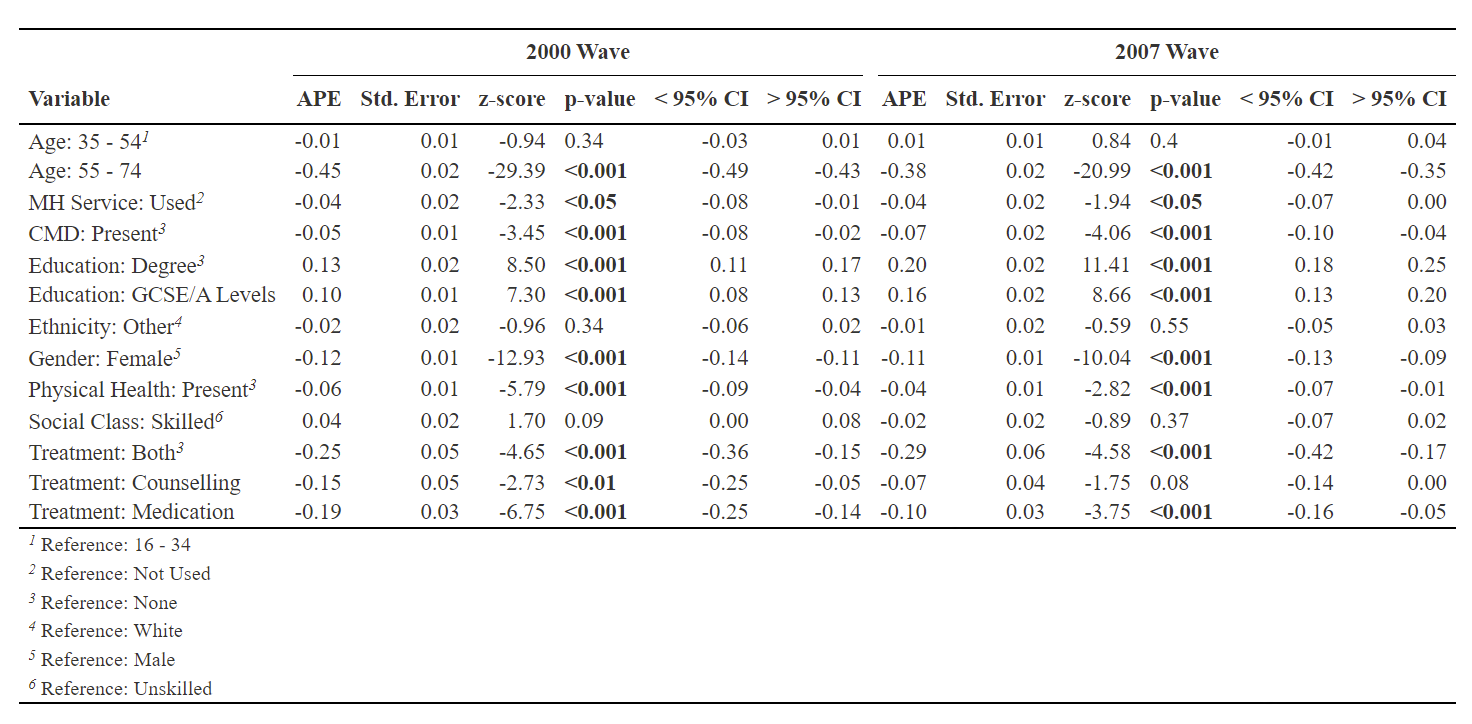
\includegraphics[width=460px,height=200px]{figure/apecmd} \caption[Average Partial Effects for for CMD]{Average Partial Effects for CMD in 2000 and 2007}\label{fig:apecmd}
\end{figure}



\begin{figure}
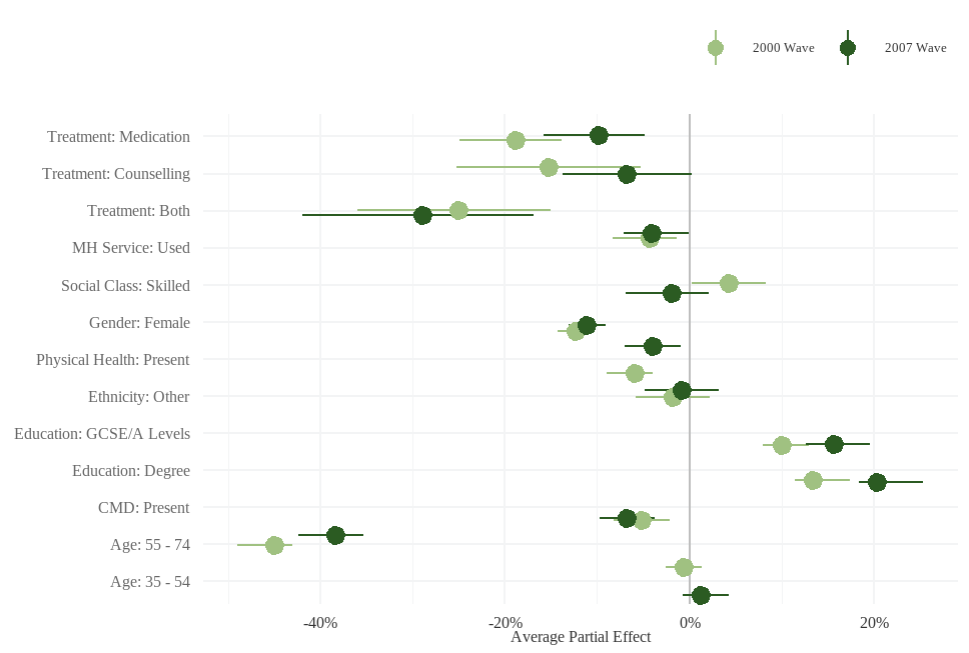
\includegraphics[width=450px,height=300px]{figure/apecmdp} \caption[Average Partial Effects Plot for CMD]{Average Partial Effects Plot for CMD in 2000 and 2007}\label{fig:apecmdp}
\end{figure}
\hypertarget{goodness-of-fit-for-common-mental-health-disorders}{%
\subsection{Goodness of Fit for Common Mental Health Disorders}\label{goodness-of-fit-for-common-mental-health-disorders}}

Figure \ref{fig:gofcmd} presents the results of diagnostic tests for the goodness of fit for each model related to common mental health disorders. The McFadden's R2 values for the 2000 and 2007 survey waves were 0.28 and 0.25 respectively, indicating a good fit for both models. The 2007 model had a slightly lower R2 value, but overall, the models with service or treatment use had a slightly better fit than the models without service or treatment use presented abovr.




\begin{figure}
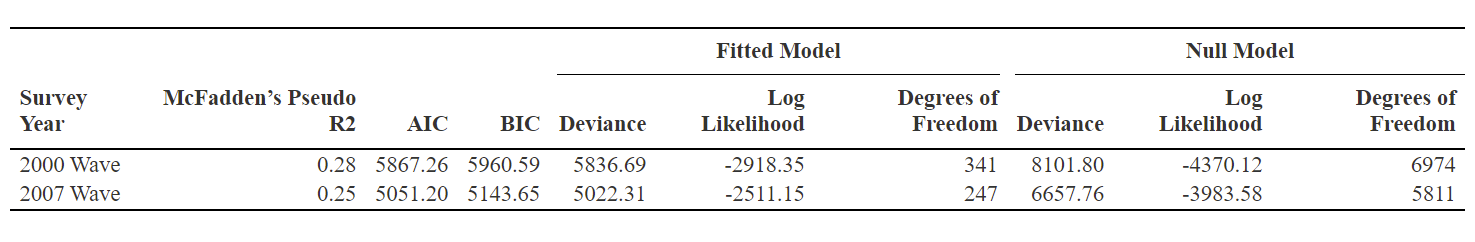
\includegraphics[width=460px,height=100px]{figure/gofcmd} \caption[Goodness of Fit for CMD Models]{Goodness of Fit for CMD Models in 2000 and 2007}\label{fig:gofcmd}
\end{figure}
\hypertarget{common-mental-health-disorder-type}{%
\section{Common Mental Health Disorder Type}\label{common-mental-health-disorder-type}}

In this section the dependent variable was again economic activity (being active or not), similar to the previous models but now with the single binary variable marking the presence or absence of common mental health disorders replaced with a set of variables relating to common mental health disorders type. These cover the conditions: depression, generalised anxiety disorder and depression (GAD), mixed anxiety and depression, obsessive compulsive disorder (OCD), panic disorder, and specific phobias. As in previous sections in this chapter, logistic regression models were applied to each survey of data, two models in total.

\hypertarget{model-results-for-type-of-common-mental-health-disorder}{%
\subsection{Model Results for Type of Common Mental Health Disorder}\label{model-results-for-type-of-common-mental-health-disorder}}

Table \ref{tab:results2-cmdtmod} details the adjusted odds rations for both of the logistic regression models. As in previous models, education was consistent across both survey waves to be positively associated and also statistically significant with being economically active. Being in the skilled social class category in the 2000 wave was also positively associated with being active, although not statistically significant. Being female, aged between 35 to 54 and 55 to 74 years old, an ethnic minority, or had a physical health condition present reduced the likelihood of being economically active.

Of the new predictor variable added, that of common mental health disorders type, all were associated with a decreased likelihood of being economically active, with depression, generalised anxiety and depression, and mixed anxiety and depression being statistically significant in the 2000 survey. OCD, panic disorder and specific phobias all had negative relationships with economic activity although they are not statistically significant. For the 2007 survey, depression, mixed anxiety and depression and specific phobias were statistically significant.

\providecommand{\huxb}[2]{\arrayrulecolor[RGB]{#1}\global\arrayrulewidth=#2pt}
  \providecommand{\huxvb}[2]{\color[RGB]{#1}\vrule width #2pt}
  \providecommand{\huxtpad}[1]{\rule{0pt}{#1}}
  \providecommand{\huxbpad}[1]{\rule[-#1]{0pt}{#1}}
\begin{table}[ht]
\begin{centerbox}
\begin{threeparttable}
 \setlength{\tabcolsep}{0pt}
\begin{adjustbox}{width=1\textwidth}
\normalsize
\begin{tabular}{l l l l l l l l l}


\hhline{>{\arrayrulecolor[RGB]{0, 0, 0}\global\arrayrulewidth=0.4pt}->{\arrayrulecolor[RGB]{0, 0, 0}\global\arrayrulewidth=0.4pt}->{\arrayrulecolor[RGB]{0, 0, 0}\global\arrayrulewidth=0.4pt}->{\arrayrulecolor[RGB]{0, 0, 0}\global\arrayrulewidth=0.4pt}->{\arrayrulecolor[RGB]{0, 0, 0}\global\arrayrulewidth=0.4pt}->{\arrayrulecolor[RGB]{0, 0, 0}\global\arrayrulewidth=0.4pt}->{\arrayrulecolor[RGB]{0, 0, 0}\global\arrayrulewidth=0.4pt}->{\arrayrulecolor[RGB]{0, 0, 0}\global\arrayrulewidth=0.4pt}->{\arrayrulecolor[RGB]{0, 0, 0}\global\arrayrulewidth=0.4pt}-}
\arrayrulecolor{black}

\multicolumn{1}{!{\color[RGB]{0, 0, 0}\vrule width 0pt}l!{\color[RGB]{0, 0, 0}\vrule width 0pt}}{\rule{0pt}{1pt + 1em}\raggedright \hspace{0pt} \textbf{{\fontsize{14pt}{16.8pt}\selectfont 
}} \hspace{1pt}\rule[-1pt]{0pt}{1pt}} &
\multicolumn{4}{c!{\color[RGB]{0, 0, 0}\vrule width 0pt}}{\rule{0pt}{1pt + 1em}\centering \hspace{1pt} \textbf{{\fontsize{14pt}{16.8pt}\selectfont \textbf{2000 Wave}
}} \hspace{1pt}\rule[-1pt]{0pt}{1pt}} &
\multicolumn{4}{c!{\color[RGB]{0, 0, 0}\vrule width 0pt}}{\rule{0pt}{1pt + 1em}\centering \hspace{1pt} \textbf{{\fontsize{14pt}{16.8pt}\selectfont \textbf{2007 Wave}
}} \hspace{1pt}\rule[-1pt]{0pt}{1pt}} \tabularnewline[-0.5pt]


\hhline{}
\arrayrulecolor{black}

\multicolumn{1}{!{\color[RGB]{0, 0, 0}\vrule width 0pt}l!{\color[RGB]{0, 0, 0}\vrule width 0pt}}{\rule{0pt}{1pt + 1em}\raggedright \hspace{0pt} \textbf{{\fontsize{14pt}{16.8pt}\selectfont \textbf{Variable}
}} \hspace{1pt}\rule[-1pt]{0pt}{1pt}} &
\multicolumn{1}{c!{\color[RGB]{0, 0, 0}\vrule width 0pt}}{\rule{0pt}{1pt + 1em}\centering \hspace{1pt} \textbf{{\fontsize{14pt}{16.8pt}\selectfont \textbf{N}
}} \hspace{1pt}\rule[-1pt]{0pt}{1pt}} &
\multicolumn{1}{c!{\color[RGB]{0, 0, 0}\vrule width 0pt}}{\rule{0pt}{1pt + 1em}\centering \hspace{1pt} \textbf{{\fontsize{14pt}{16.8pt}\selectfont \textbf{OR}
}} \hspace{1pt}\rule[-1pt]{0pt}{1pt}} &
\multicolumn{1}{c!{\color[RGB]{0, 0, 0}\vrule width 0pt}}{\rule{0pt}{1pt + 1em}\centering \hspace{1pt} \textbf{{\fontsize{14pt}{16.8pt}\selectfont \textbf{95\% CI}
}} \hspace{1pt}\rule[-1pt]{0pt}{1pt}} &
\multicolumn{1}{c!{\color[RGB]{0, 0, 0}\vrule width 0pt}}{\rule{0pt}{1pt + 1em}\centering \hspace{1pt} \textbf{{\fontsize{14pt}{16.8pt}\selectfont \textbf{p-value}
}} \hspace{1pt}\rule[-1pt]{0pt}{1pt}} &
\multicolumn{1}{c!{\color[RGB]{0, 0, 0}\vrule width 0pt}}{\rule{0pt}{1pt + 1em}\centering \hspace{1pt} \textbf{{\fontsize{14pt}{16.8pt}\selectfont \textbf{N}
}} \hspace{1pt}\rule[-1pt]{0pt}{1pt}} &
\multicolumn{1}{c!{\color[RGB]{0, 0, 0}\vrule width 0pt}}{\rule{0pt}{1pt + 1em}\centering \hspace{1pt} \textbf{{\fontsize{14pt}{16.8pt}\selectfont \textbf{OR}
}} \hspace{1pt}\rule[-1pt]{0pt}{1pt}} &
\multicolumn{1}{c!{\color[RGB]{0, 0, 0}\vrule width 0pt}}{\rule{0pt}{1pt + 1em}\centering \hspace{1pt} \textbf{{\fontsize{14pt}{16.8pt}\selectfont \textbf{95\% CI}
}} \hspace{1pt}\rule[-1pt]{0pt}{1pt}} &
\multicolumn{1}{c!{\color[RGB]{0, 0, 0}\vrule width 0pt}}{\rule{0pt}{1pt + 1em}\centering \hspace{1pt} \textbf{{\fontsize{14pt}{16.8pt}\selectfont \textbf{p-value}
}} \hspace{0pt}\rule[-1pt]{0pt}{1pt}} \tabularnewline[-0.5pt]


\hhline{>{\arrayrulecolor[RGB]{0, 0, 0}\global\arrayrulewidth=0.4pt}->{\arrayrulecolor[RGB]{0, 0, 0}\global\arrayrulewidth=0.4pt}->{\arrayrulecolor[RGB]{0, 0, 0}\global\arrayrulewidth=0.4pt}->{\arrayrulecolor[RGB]{0, 0, 0}\global\arrayrulewidth=0.4pt}->{\arrayrulecolor[RGB]{0, 0, 0}\global\arrayrulewidth=0.4pt}->{\arrayrulecolor[RGB]{0, 0, 0}\global\arrayrulewidth=0.4pt}->{\arrayrulecolor[RGB]{0, 0, 0}\global\arrayrulewidth=0.4pt}->{\arrayrulecolor[RGB]{0, 0, 0}\global\arrayrulewidth=0.4pt}->{\arrayrulecolor[RGB]{0, 0, 0}\global\arrayrulewidth=0.4pt}-}
\arrayrulecolor{black}

\multicolumn{1}{!{\color[RGB]{0, 0, 0}\vrule width 0pt}l!{\color[RGB]{0, 0, 0}\vrule width 0pt}}{\rule{0pt}{1pt + 1em}\raggedright \hspace{0pt} \textbf{{\fontsize{14pt}{16.8pt}\selectfont CMD Type}} \hspace{1pt}\rule[-1pt]{0pt}{1pt}} &
\multicolumn{1}{c!{\color[RGB]{0, 0, 0}\vrule width 0pt}}{\rule{0pt}{1pt + 1em}\centering \hspace{1pt} {\fontsize{14pt}{16.8pt}\selectfont 6,920} \hspace{1pt}\rule[-1pt]{0pt}{1pt}} &
\multicolumn{1}{c!{\color[RGB]{0, 0, 0}\vrule width 0pt}}{\rule{0pt}{1pt + 1em}\centering \hspace{1pt} {\fontsize{14pt}{16.8pt}\selectfont } \hspace{1pt}\rule[-1pt]{0pt}{1pt}} &
\multicolumn{1}{c!{\color[RGB]{0, 0, 0}\vrule width 0pt}}{\rule{0pt}{1pt + 1em}\centering \hspace{1pt} {\fontsize{14pt}{16.8pt}\selectfont } \hspace{1pt}\rule[-1pt]{0pt}{1pt}} &
\multicolumn{1}{c!{\color[RGB]{0, 0, 0}\vrule width 0pt}}{\rule{0pt}{1pt + 1em}\centering \hspace{1pt} {\fontsize{14pt}{16.8pt}\selectfont } \hspace{1pt}\rule[-1pt]{0pt}{1pt}} &
\multicolumn{1}{c!{\color[RGB]{0, 0, 0}\vrule width 0pt}}{\rule{0pt}{1pt + 1em}\centering \hspace{1pt} {\fontsize{14pt}{16.8pt}\selectfont 5,750} \hspace{1pt}\rule[-1pt]{0pt}{1pt}} &
\multicolumn{1}{c!{\color[RGB]{0, 0, 0}\vrule width 0pt}}{\rule{0pt}{1pt + 1em}\centering \hspace{1pt} {\fontsize{14pt}{16.8pt}\selectfont } \hspace{1pt}\rule[-1pt]{0pt}{1pt}} &
\multicolumn{1}{c!{\color[RGB]{0, 0, 0}\vrule width 0pt}}{\rule{0pt}{1pt + 1em}\centering \hspace{1pt} {\fontsize{14pt}{16.8pt}\selectfont } \hspace{1pt}\rule[-1pt]{0pt}{1pt}} &
\multicolumn{1}{c!{\color[RGB]{0, 0, 0}\vrule width 0pt}}{\rule{0pt}{1pt + 1em}\centering \hspace{1pt} {\fontsize{14pt}{16.8pt}\selectfont } \hspace{0pt}\rule[-1pt]{0pt}{1pt}} \tabularnewline[-0.5pt]


\hhline{}
\arrayrulecolor{black}

\multicolumn{1}{!{\color[RGB]{0, 0, 0}\vrule width 0pt}l!{\color[RGB]{0, 0, 0}\vrule width 0pt}}{\rule{0pt}{1pt + 1em}\raggedright \hspace{0pt} {\fontsize{14pt}{16.8pt}\selectfont None} \hspace{1pt}\rule[-1pt]{0pt}{1pt}} &
\multicolumn{1}{c!{\color[RGB]{0, 0, 0}\vrule width 0pt}}{\rule{0pt}{1pt + 1em}\centering \hspace{1pt} {\fontsize{14pt}{16.8pt}\selectfont } \hspace{1pt}\rule[-1pt]{0pt}{1pt}} &
\multicolumn{1}{c!{\color[RGB]{0, 0, 0}\vrule width 0pt}}{\rule{0pt}{1pt + 1em}\centering \hspace{1pt} {\fontsize{14pt}{16.8pt}\selectfont —} \hspace{1pt}\rule[-1pt]{0pt}{1pt}} &
\multicolumn{1}{c!{\color[RGB]{0, 0, 0}\vrule width 0pt}}{\rule{0pt}{1pt + 1em}\centering \hspace{1pt} {\fontsize{14pt}{16.8pt}\selectfont —} \hspace{1pt}\rule[-1pt]{0pt}{1pt}} &
\multicolumn{1}{c!{\color[RGB]{0, 0, 0}\vrule width 0pt}}{\rule{0pt}{1pt + 1em}\centering \hspace{1pt} {\fontsize{14pt}{16.8pt}\selectfont } \hspace{1pt}\rule[-1pt]{0pt}{1pt}} &
\multicolumn{1}{c!{\color[RGB]{0, 0, 0}\vrule width 0pt}}{\rule{0pt}{1pt + 1em}\centering \hspace{1pt} {\fontsize{14pt}{16.8pt}\selectfont } \hspace{1pt}\rule[-1pt]{0pt}{1pt}} &
\multicolumn{1}{c!{\color[RGB]{0, 0, 0}\vrule width 0pt}}{\rule{0pt}{1pt + 1em}\centering \hspace{1pt} {\fontsize{14pt}{16.8pt}\selectfont —} \hspace{1pt}\rule[-1pt]{0pt}{1pt}} &
\multicolumn{1}{c!{\color[RGB]{0, 0, 0}\vrule width 0pt}}{\rule{0pt}{1pt + 1em}\centering \hspace{1pt} {\fontsize{14pt}{16.8pt}\selectfont —} \hspace{1pt}\rule[-1pt]{0pt}{1pt}} &
\multicolumn{1}{c!{\color[RGB]{0, 0, 0}\vrule width 0pt}}{\rule{0pt}{1pt + 1em}\centering \hspace{1pt} {\fontsize{14pt}{16.8pt}\selectfont } \hspace{0pt}\rule[-1pt]{0pt}{1pt}} \tabularnewline[-0.5pt]


\hhline{}
\arrayrulecolor{black}

\multicolumn{1}{!{\color[RGB]{0, 0, 0}\vrule width 0pt}l!{\color[RGB]{0, 0, 0}\vrule width 0pt}}{\rule{0pt}{1pt + 1em}\raggedright \hspace{0pt} {\fontsize{14pt}{16.8pt}\selectfont Dep Episode} \hspace{1pt}\rule[-1pt]{0pt}{1pt}} &
\multicolumn{1}{c!{\color[RGB]{0, 0, 0}\vrule width 0pt}}{\rule{0pt}{1pt + 1em}\centering \hspace{1pt} {\fontsize{14pt}{16.8pt}\selectfont } \hspace{1pt}\rule[-1pt]{0pt}{1pt}} &
\multicolumn{1}{c!{\color[RGB]{0, 0, 0}\vrule width 0pt}}{\rule{0pt}{1pt + 1em}\centering \hspace{1pt} {\fontsize{14pt}{16.8pt}\selectfont 0.43} \hspace{1pt}\rule[-1pt]{0pt}{1pt}} &
\multicolumn{1}{c!{\color[RGB]{0, 0, 0}\vrule width 0pt}}{\rule{0pt}{1pt + 1em}\centering \hspace{1pt} {\fontsize{14pt}{16.8pt}\selectfont 0.25, 0.72} \hspace{1pt}\rule[-1pt]{0pt}{1pt}} &
\multicolumn{1}{c!{\color[RGB]{0, 0, 0}\vrule width 0pt}}{\rule{0pt}{1pt + 1em}\centering \hspace{1pt} \textbf{{\fontsize{14pt}{16.8pt}\selectfont 0.001}} \hspace{1pt}\rule[-1pt]{0pt}{1pt}} &
\multicolumn{1}{c!{\color[RGB]{0, 0, 0}\vrule width 0pt}}{\rule{0pt}{1pt + 1em}\centering \hspace{1pt} {\fontsize{14pt}{16.8pt}\selectfont } \hspace{1pt}\rule[-1pt]{0pt}{1pt}} &
\multicolumn{1}{c!{\color[RGB]{0, 0, 0}\vrule width 0pt}}{\rule{0pt}{1pt + 1em}\centering \hspace{1pt} {\fontsize{14pt}{16.8pt}\selectfont 0.25} \hspace{1pt}\rule[-1pt]{0pt}{1pt}} &
\multicolumn{1}{c!{\color[RGB]{0, 0, 0}\vrule width 0pt}}{\rule{0pt}{1pt + 1em}\centering \hspace{1pt} {\fontsize{14pt}{16.8pt}\selectfont 0.17, 0.36} \hspace{1pt}\rule[-1pt]{0pt}{1pt}} &
\multicolumn{1}{c!{\color[RGB]{0, 0, 0}\vrule width 0pt}}{\rule{0pt}{1pt + 1em}\centering \hspace{1pt} \textbf{{\fontsize{14pt}{16.8pt}\selectfont $<$0.001}} \hspace{0pt}\rule[-1pt]{0pt}{1pt}} \tabularnewline[-0.5pt]


\hhline{}
\arrayrulecolor{black}

\multicolumn{1}{!{\color[RGB]{0, 0, 0}\vrule width 0pt}l!{\color[RGB]{0, 0, 0}\vrule width 0pt}}{\rule{0pt}{1pt + 1em}\raggedright \hspace{0pt} {\fontsize{14pt}{16.8pt}\selectfont Gen Anx \& Dep} \hspace{1pt}\rule[-1pt]{0pt}{1pt}} &
\multicolumn{1}{c!{\color[RGB]{0, 0, 0}\vrule width 0pt}}{\rule{0pt}{1pt + 1em}\centering \hspace{1pt} {\fontsize{14pt}{16.8pt}\selectfont } \hspace{1pt}\rule[-1pt]{0pt}{1pt}} &
\multicolumn{1}{c!{\color[RGB]{0, 0, 0}\vrule width 0pt}}{\rule{0pt}{1pt + 1em}\centering \hspace{1pt} {\fontsize{14pt}{16.8pt}\selectfont 0.32} \hspace{1pt}\rule[-1pt]{0pt}{1pt}} &
\multicolumn{1}{c!{\color[RGB]{0, 0, 0}\vrule width 0pt}}{\rule{0pt}{1pt + 1em}\centering \hspace{1pt} {\fontsize{14pt}{16.8pt}\selectfont 0.24, 0.44} \hspace{1pt}\rule[-1pt]{0pt}{1pt}} &
\multicolumn{1}{c!{\color[RGB]{0, 0, 0}\vrule width 0pt}}{\rule{0pt}{1pt + 1em}\centering \hspace{1pt} \textbf{{\fontsize{14pt}{16.8pt}\selectfont $<$0.001}} \hspace{1pt}\rule[-1pt]{0pt}{1pt}} &
\multicolumn{1}{c!{\color[RGB]{0, 0, 0}\vrule width 0pt}}{\rule{0pt}{1pt + 1em}\centering \hspace{1pt} {\fontsize{14pt}{16.8pt}\selectfont } \hspace{1pt}\rule[-1pt]{0pt}{1pt}} &
\multicolumn{1}{c!{\color[RGB]{0, 0, 0}\vrule width 0pt}}{\rule{0pt}{1pt + 1em}\centering \hspace{1pt} {\fontsize{14pt}{16.8pt}\selectfont 0.73} \hspace{1pt}\rule[-1pt]{0pt}{1pt}} &
\multicolumn{1}{c!{\color[RGB]{0, 0, 0}\vrule width 0pt}}{\rule{0pt}{1pt + 1em}\centering \hspace{1pt} {\fontsize{14pt}{16.8pt}\selectfont 0.48, 1.12} \hspace{1pt}\rule[-1pt]{0pt}{1pt}} &
\multicolumn{1}{c!{\color[RGB]{0, 0, 0}\vrule width 0pt}}{\rule{0pt}{1pt + 1em}\centering \hspace{1pt} {\fontsize{14pt}{16.8pt}\selectfont 0.15} \hspace{0pt}\rule[-1pt]{0pt}{1pt}} \tabularnewline[-0.5pt]


\hhline{}
\arrayrulecolor{black}

\multicolumn{1}{!{\color[RGB]{0, 0, 0}\vrule width 0pt}l!{\color[RGB]{0, 0, 0}\vrule width 0pt}}{\rule{0pt}{1pt + 1em}\raggedright \hspace{0pt} {\fontsize{14pt}{16.8pt}\selectfont Mixed Anx \& Dep} \hspace{1pt}\rule[-1pt]{0pt}{1pt}} &
\multicolumn{1}{c!{\color[RGB]{0, 0, 0}\vrule width 0pt}}{\rule{0pt}{1pt + 1em}\centering \hspace{1pt} {\fontsize{14pt}{16.8pt}\selectfont } \hspace{1pt}\rule[-1pt]{0pt}{1pt}} &
\multicolumn{1}{c!{\color[RGB]{0, 0, 0}\vrule width 0pt}}{\rule{0pt}{1pt + 1em}\centering \hspace{1pt} {\fontsize{14pt}{16.8pt}\selectfont 0.61} \hspace{1pt}\rule[-1pt]{0pt}{1pt}} &
\multicolumn{1}{c!{\color[RGB]{0, 0, 0}\vrule width 0pt}}{\rule{0pt}{1pt + 1em}\centering \hspace{1pt} {\fontsize{14pt}{16.8pt}\selectfont 0.48, 0.78} \hspace{1pt}\rule[-1pt]{0pt}{1pt}} &
\multicolumn{1}{c!{\color[RGB]{0, 0, 0}\vrule width 0pt}}{\rule{0pt}{1pt + 1em}\centering \hspace{1pt} \textbf{{\fontsize{14pt}{16.8pt}\selectfont $<$0.001}} \hspace{1pt}\rule[-1pt]{0pt}{1pt}} &
\multicolumn{1}{c!{\color[RGB]{0, 0, 0}\vrule width 0pt}}{\rule{0pt}{1pt + 1em}\centering \hspace{1pt} {\fontsize{14pt}{16.8pt}\selectfont } \hspace{1pt}\rule[-1pt]{0pt}{1pt}} &
\multicolumn{1}{c!{\color[RGB]{0, 0, 0}\vrule width 0pt}}{\rule{0pt}{1pt + 1em}\centering \hspace{1pt} {\fontsize{14pt}{16.8pt}\selectfont 0.54} \hspace{1pt}\rule[-1pt]{0pt}{1pt}} &
\multicolumn{1}{c!{\color[RGB]{0, 0, 0}\vrule width 0pt}}{\rule{0pt}{1pt + 1em}\centering \hspace{1pt} {\fontsize{14pt}{16.8pt}\selectfont 0.41, 0.69} \hspace{1pt}\rule[-1pt]{0pt}{1pt}} &
\multicolumn{1}{c!{\color[RGB]{0, 0, 0}\vrule width 0pt}}{\rule{0pt}{1pt + 1em}\centering \hspace{1pt} \textbf{{\fontsize{14pt}{16.8pt}\selectfont $<$0.001}} \hspace{0pt}\rule[-1pt]{0pt}{1pt}} \tabularnewline[-0.5pt]


\hhline{}
\arrayrulecolor{black}

\multicolumn{1}{!{\color[RGB]{0, 0, 0}\vrule width 0pt}l!{\color[RGB]{0, 0, 0}\vrule width 0pt}}{\rule{0pt}{1pt + 1em}\raggedright \hspace{0pt} {\fontsize{14pt}{16.8pt}\selectfont OCD} \hspace{1pt}\rule[-1pt]{0pt}{1pt}} &
\multicolumn{1}{c!{\color[RGB]{0, 0, 0}\vrule width 0pt}}{\rule{0pt}{1pt + 1em}\centering \hspace{1pt} {\fontsize{14pt}{16.8pt}\selectfont } \hspace{1pt}\rule[-1pt]{0pt}{1pt}} &
\multicolumn{1}{c!{\color[RGB]{0, 0, 0}\vrule width 0pt}}{\rule{0pt}{1pt + 1em}\centering \hspace{1pt} {\fontsize{14pt}{16.8pt}\selectfont 0.54} \hspace{1pt}\rule[-1pt]{0pt}{1pt}} &
\multicolumn{1}{c!{\color[RGB]{0, 0, 0}\vrule width 0pt}}{\rule{0pt}{1pt + 1em}\centering \hspace{1pt} {\fontsize{14pt}{16.8pt}\selectfont 0.24, 1.26} \hspace{1pt}\rule[-1pt]{0pt}{1pt}} &
\multicolumn{1}{c!{\color[RGB]{0, 0, 0}\vrule width 0pt}}{\rule{0pt}{1pt + 1em}\centering \hspace{1pt} {\fontsize{14pt}{16.8pt}\selectfont 0.16} \hspace{1pt}\rule[-1pt]{0pt}{1pt}} &
\multicolumn{1}{c!{\color[RGB]{0, 0, 0}\vrule width 0pt}}{\rule{0pt}{1pt + 1em}\centering \hspace{1pt} {\fontsize{14pt}{16.8pt}\selectfont } \hspace{1pt}\rule[-1pt]{0pt}{1pt}} &
\multicolumn{1}{c!{\color[RGB]{0, 0, 0}\vrule width 0pt}}{\rule{0pt}{1pt + 1em}\centering \hspace{1pt} {\fontsize{14pt}{16.8pt}\selectfont 0.84} \hspace{1pt}\rule[-1pt]{0pt}{1pt}} &
\multicolumn{1}{c!{\color[RGB]{0, 0, 0}\vrule width 0pt}}{\rule{0pt}{1pt + 1em}\centering \hspace{1pt} {\fontsize{14pt}{16.8pt}\selectfont 0.26, 2.70} \hspace{1pt}\rule[-1pt]{0pt}{1pt}} &
\multicolumn{1}{c!{\color[RGB]{0, 0, 0}\vrule width 0pt}}{\rule{0pt}{1pt + 1em}\centering \hspace{1pt} {\fontsize{14pt}{16.8pt}\selectfont 0.77} \hspace{0pt}\rule[-1pt]{0pt}{1pt}} \tabularnewline[-0.5pt]


\hhline{}
\arrayrulecolor{black}

\multicolumn{1}{!{\color[RGB]{0, 0, 0}\vrule width 0pt}l!{\color[RGB]{0, 0, 0}\vrule width 0pt}}{\rule{0pt}{1pt + 1em}\raggedright \hspace{0pt} {\fontsize{14pt}{16.8pt}\selectfont Panic Dis} \hspace{1pt}\rule[-1pt]{0pt}{1pt}} &
\multicolumn{1}{c!{\color[RGB]{0, 0, 0}\vrule width 0pt}}{\rule{0pt}{1pt + 1em}\centering \hspace{1pt} {\fontsize{14pt}{16.8pt}\selectfont } \hspace{1pt}\rule[-1pt]{0pt}{1pt}} &
\multicolumn{1}{c!{\color[RGB]{0, 0, 0}\vrule width 0pt}}{\rule{0pt}{1pt + 1em}\centering \hspace{1pt} {\fontsize{14pt}{16.8pt}\selectfont 0.69} \hspace{1pt}\rule[-1pt]{0pt}{1pt}} &
\multicolumn{1}{c!{\color[RGB]{0, 0, 0}\vrule width 0pt}}{\rule{0pt}{1pt + 1em}\centering \hspace{1pt} {\fontsize{14pt}{16.8pt}\selectfont 0.26, 1.87} \hspace{1pt}\rule[-1pt]{0pt}{1pt}} &
\multicolumn{1}{c!{\color[RGB]{0, 0, 0}\vrule width 0pt}}{\rule{0pt}{1pt + 1em}\centering \hspace{1pt} {\fontsize{14pt}{16.8pt}\selectfont 0.46} \hspace{1pt}\rule[-1pt]{0pt}{1pt}} &
\multicolumn{1}{c!{\color[RGB]{0, 0, 0}\vrule width 0pt}}{\rule{0pt}{1pt + 1em}\centering \hspace{1pt} {\fontsize{14pt}{16.8pt}\selectfont } \hspace{1pt}\rule[-1pt]{0pt}{1pt}} &
\multicolumn{1}{c!{\color[RGB]{0, 0, 0}\vrule width 0pt}}{\rule{0pt}{1pt + 1em}\centering \hspace{1pt} {\fontsize{14pt}{16.8pt}\selectfont 0.81} \hspace{1pt}\rule[-1pt]{0pt}{1pt}} &
\multicolumn{1}{c!{\color[RGB]{0, 0, 0}\vrule width 0pt}}{\rule{0pt}{1pt + 1em}\centering \hspace{1pt} {\fontsize{14pt}{16.8pt}\selectfont 0.38, 1.70} \hspace{1pt}\rule[-1pt]{0pt}{1pt}} &
\multicolumn{1}{c!{\color[RGB]{0, 0, 0}\vrule width 0pt}}{\rule{0pt}{1pt + 1em}\centering \hspace{1pt} {\fontsize{14pt}{16.8pt}\selectfont 0.57} \hspace{0pt}\rule[-1pt]{0pt}{1pt}} \tabularnewline[-0.5pt]


\hhline{}
\arrayrulecolor{black}

\multicolumn{1}{!{\color[RGB]{0, 0, 0}\vrule width 0pt}l!{\color[RGB]{0, 0, 0}\vrule width 0pt}}{\rule{0pt}{1pt + 1em}\raggedright \hspace{0pt} {\fontsize{14pt}{16.8pt}\selectfont Specific Phob} \hspace{1pt}\rule[-1pt]{0pt}{1pt}} &
\multicolumn{1}{c!{\color[RGB]{0, 0, 0}\vrule width 0pt}}{\rule{0pt}{1pt + 1em}\centering \hspace{1pt} {\fontsize{14pt}{16.8pt}\selectfont } \hspace{1pt}\rule[-1pt]{0pt}{1pt}} &
\multicolumn{1}{c!{\color[RGB]{0, 0, 0}\vrule width 0pt}}{\rule{0pt}{1pt + 1em}\centering \hspace{1pt} {\fontsize{14pt}{16.8pt}\selectfont 0.49} \hspace{1pt}\rule[-1pt]{0pt}{1pt}} &
\multicolumn{1}{c!{\color[RGB]{0, 0, 0}\vrule width 0pt}}{\rule{0pt}{1pt + 1em}\centering \hspace{1pt} {\fontsize{14pt}{16.8pt}\selectfont 0.24, 1.02} \hspace{1pt}\rule[-1pt]{0pt}{1pt}} &
\multicolumn{1}{c!{\color[RGB]{0, 0, 0}\vrule width 0pt}}{\rule{0pt}{1pt + 1em}\centering \hspace{1pt} {\fontsize{14pt}{16.8pt}\selectfont 0.057} \hspace{1pt}\rule[-1pt]{0pt}{1pt}} &
\multicolumn{1}{c!{\color[RGB]{0, 0, 0}\vrule width 0pt}}{\rule{0pt}{1pt + 1em}\centering \hspace{1pt} {\fontsize{14pt}{16.8pt}\selectfont } \hspace{1pt}\rule[-1pt]{0pt}{1pt}} &
\multicolumn{1}{c!{\color[RGB]{0, 0, 0}\vrule width 0pt}}{\rule{0pt}{1pt + 1em}\centering \hspace{1pt} {\fontsize{14pt}{16.8pt}\selectfont 0.33} \hspace{1pt}\rule[-1pt]{0pt}{1pt}} &
\multicolumn{1}{c!{\color[RGB]{0, 0, 0}\vrule width 0pt}}{\rule{0pt}{1pt + 1em}\centering \hspace{1pt} {\fontsize{14pt}{16.8pt}\selectfont 0.16, 0.69} \hspace{1pt}\rule[-1pt]{0pt}{1pt}} &
\multicolumn{1}{c!{\color[RGB]{0, 0, 0}\vrule width 0pt}}{\rule{0pt}{1pt + 1em}\centering \hspace{1pt} \textbf{{\fontsize{14pt}{16.8pt}\selectfont 0.003}} \hspace{0pt}\rule[-1pt]{0pt}{1pt}} \tabularnewline[-0.5pt]


\hhline{}
\arrayrulecolor{black}

\multicolumn{1}{!{\color[RGB]{0, 0, 0}\vrule width 0pt}l!{\color[RGB]{0, 0, 0}\vrule width 0pt}}{\rule{0pt}{1pt + 1em}\raggedright \hspace{0pt} \textbf{{\fontsize{14pt}{16.8pt}\selectfont Gender}} \hspace{1pt}\rule[-1pt]{0pt}{1pt}} &
\multicolumn{1}{c!{\color[RGB]{0, 0, 0}\vrule width 0pt}}{\rule{0pt}{1pt + 1em}\centering \hspace{1pt} {\fontsize{14pt}{16.8pt}\selectfont 6,920} \hspace{1pt}\rule[-1pt]{0pt}{1pt}} &
\multicolumn{1}{c!{\color[RGB]{0, 0, 0}\vrule width 0pt}}{\rule{0pt}{1pt + 1em}\centering \hspace{1pt} {\fontsize{14pt}{16.8pt}\selectfont } \hspace{1pt}\rule[-1pt]{0pt}{1pt}} &
\multicolumn{1}{c!{\color[RGB]{0, 0, 0}\vrule width 0pt}}{\rule{0pt}{1pt + 1em}\centering \hspace{1pt} {\fontsize{14pt}{16.8pt}\selectfont } \hspace{1pt}\rule[-1pt]{0pt}{1pt}} &
\multicolumn{1}{c!{\color[RGB]{0, 0, 0}\vrule width 0pt}}{\rule{0pt}{1pt + 1em}\centering \hspace{1pt} {\fontsize{14pt}{16.8pt}\selectfont } \hspace{1pt}\rule[-1pt]{0pt}{1pt}} &
\multicolumn{1}{c!{\color[RGB]{0, 0, 0}\vrule width 0pt}}{\rule{0pt}{1pt + 1em}\centering \hspace{1pt} {\fontsize{14pt}{16.8pt}\selectfont 5,750} \hspace{1pt}\rule[-1pt]{0pt}{1pt}} &
\multicolumn{1}{c!{\color[RGB]{0, 0, 0}\vrule width 0pt}}{\rule{0pt}{1pt + 1em}\centering \hspace{1pt} {\fontsize{14pt}{16.8pt}\selectfont } \hspace{1pt}\rule[-1pt]{0pt}{1pt}} &
\multicolumn{1}{c!{\color[RGB]{0, 0, 0}\vrule width 0pt}}{\rule{0pt}{1pt + 1em}\centering \hspace{1pt} {\fontsize{14pt}{16.8pt}\selectfont } \hspace{1pt}\rule[-1pt]{0pt}{1pt}} &
\multicolumn{1}{c!{\color[RGB]{0, 0, 0}\vrule width 0pt}}{\rule{0pt}{1pt + 1em}\centering \hspace{1pt} {\fontsize{14pt}{16.8pt}\selectfont } \hspace{0pt}\rule[-1pt]{0pt}{1pt}} \tabularnewline[-0.5pt]


\hhline{}
\arrayrulecolor{black}

\multicolumn{1}{!{\color[RGB]{0, 0, 0}\vrule width 0pt}l!{\color[RGB]{0, 0, 0}\vrule width 0pt}}{\rule{0pt}{1pt + 1em}\raggedright \hspace{0pt} {\fontsize{14pt}{16.8pt}\selectfont Male} \hspace{1pt}\rule[-1pt]{0pt}{1pt}} &
\multicolumn{1}{c!{\color[RGB]{0, 0, 0}\vrule width 0pt}}{\rule{0pt}{1pt + 1em}\centering \hspace{1pt} {\fontsize{14pt}{16.8pt}\selectfont } \hspace{1pt}\rule[-1pt]{0pt}{1pt}} &
\multicolumn{1}{c!{\color[RGB]{0, 0, 0}\vrule width 0pt}}{\rule{0pt}{1pt + 1em}\centering \hspace{1pt} {\fontsize{14pt}{16.8pt}\selectfont —} \hspace{1pt}\rule[-1pt]{0pt}{1pt}} &
\multicolumn{1}{c!{\color[RGB]{0, 0, 0}\vrule width 0pt}}{\rule{0pt}{1pt + 1em}\centering \hspace{1pt} {\fontsize{14pt}{16.8pt}\selectfont —} \hspace{1pt}\rule[-1pt]{0pt}{1pt}} &
\multicolumn{1}{c!{\color[RGB]{0, 0, 0}\vrule width 0pt}}{\rule{0pt}{1pt + 1em}\centering \hspace{1pt} {\fontsize{14pt}{16.8pt}\selectfont } \hspace{1pt}\rule[-1pt]{0pt}{1pt}} &
\multicolumn{1}{c!{\color[RGB]{0, 0, 0}\vrule width 0pt}}{\rule{0pt}{1pt + 1em}\centering \hspace{1pt} {\fontsize{14pt}{16.8pt}\selectfont } \hspace{1pt}\rule[-1pt]{0pt}{1pt}} &
\multicolumn{1}{c!{\color[RGB]{0, 0, 0}\vrule width 0pt}}{\rule{0pt}{1pt + 1em}\centering \hspace{1pt} {\fontsize{14pt}{16.8pt}\selectfont —} \hspace{1pt}\rule[-1pt]{0pt}{1pt}} &
\multicolumn{1}{c!{\color[RGB]{0, 0, 0}\vrule width 0pt}}{\rule{0pt}{1pt + 1em}\centering \hspace{1pt} {\fontsize{14pt}{16.8pt}\selectfont —} \hspace{1pt}\rule[-1pt]{0pt}{1pt}} &
\multicolumn{1}{c!{\color[RGB]{0, 0, 0}\vrule width 0pt}}{\rule{0pt}{1pt + 1em}\centering \hspace{1pt} {\fontsize{14pt}{16.8pt}\selectfont } \hspace{0pt}\rule[-1pt]{0pt}{1pt}} \tabularnewline[-0.5pt]


\hhline{}
\arrayrulecolor{black}

\multicolumn{1}{!{\color[RGB]{0, 0, 0}\vrule width 0pt}l!{\color[RGB]{0, 0, 0}\vrule width 0pt}}{\rule{0pt}{1pt + 1em}\raggedright \hspace{0pt} {\fontsize{14pt}{16.8pt}\selectfont Female} \hspace{1pt}\rule[-1pt]{0pt}{1pt}} &
\multicolumn{1}{c!{\color[RGB]{0, 0, 0}\vrule width 0pt}}{\rule{0pt}{1pt + 1em}\centering \hspace{1pt} {\fontsize{14pt}{16.8pt}\selectfont } \hspace{1pt}\rule[-1pt]{0pt}{1pt}} &
\multicolumn{1}{c!{\color[RGB]{0, 0, 0}\vrule width 0pt}}{\rule{0pt}{1pt + 1em}\centering \hspace{1pt} {\fontsize{14pt}{16.8pt}\selectfont 0.39} \hspace{1pt}\rule[-1pt]{0pt}{1pt}} &
\multicolumn{1}{c!{\color[RGB]{0, 0, 0}\vrule width 0pt}}{\rule{0pt}{1pt + 1em}\centering \hspace{1pt} {\fontsize{14pt}{16.8pt}\selectfont 0.34, 0.45} \hspace{1pt}\rule[-1pt]{0pt}{1pt}} &
\multicolumn{1}{c!{\color[RGB]{0, 0, 0}\vrule width 0pt}}{\rule{0pt}{1pt + 1em}\centering \hspace{1pt} \textbf{{\fontsize{14pt}{16.8pt}\selectfont $<$0.001}} \hspace{1pt}\rule[-1pt]{0pt}{1pt}} &
\multicolumn{1}{c!{\color[RGB]{0, 0, 0}\vrule width 0pt}}{\rule{0pt}{1pt + 1em}\centering \hspace{1pt} {\fontsize{14pt}{16.8pt}\selectfont } \hspace{1pt}\rule[-1pt]{0pt}{1pt}} &
\multicolumn{1}{c!{\color[RGB]{0, 0, 0}\vrule width 0pt}}{\rule{0pt}{1pt + 1em}\centering \hspace{1pt} {\fontsize{14pt}{16.8pt}\selectfont 0.46} \hspace{1pt}\rule[-1pt]{0pt}{1pt}} &
\multicolumn{1}{c!{\color[RGB]{0, 0, 0}\vrule width 0pt}}{\rule{0pt}{1pt + 1em}\centering \hspace{1pt} {\fontsize{14pt}{16.8pt}\selectfont 0.40, 0.53} \hspace{1pt}\rule[-1pt]{0pt}{1pt}} &
\multicolumn{1}{c!{\color[RGB]{0, 0, 0}\vrule width 0pt}}{\rule{0pt}{1pt + 1em}\centering \hspace{1pt} \textbf{{\fontsize{14pt}{16.8pt}\selectfont $<$0.001}} \hspace{0pt}\rule[-1pt]{0pt}{1pt}} \tabularnewline[-0.5pt]


\hhline{}
\arrayrulecolor{black}

\multicolumn{1}{!{\color[RGB]{0, 0, 0}\vrule width 0pt}l!{\color[RGB]{0, 0, 0}\vrule width 0pt}}{\rule{0pt}{1pt + 1em}\raggedright \hspace{0pt} \textbf{{\fontsize{14pt}{16.8pt}\selectfont Age Band}} \hspace{1pt}\rule[-1pt]{0pt}{1pt}} &
\multicolumn{1}{c!{\color[RGB]{0, 0, 0}\vrule width 0pt}}{\rule{0pt}{1pt + 1em}\centering \hspace{1pt} {\fontsize{14pt}{16.8pt}\selectfont 6,920} \hspace{1pt}\rule[-1pt]{0pt}{1pt}} &
\multicolumn{1}{c!{\color[RGB]{0, 0, 0}\vrule width 0pt}}{\rule{0pt}{1pt + 1em}\centering \hspace{1pt} {\fontsize{14pt}{16.8pt}\selectfont } \hspace{1pt}\rule[-1pt]{0pt}{1pt}} &
\multicolumn{1}{c!{\color[RGB]{0, 0, 0}\vrule width 0pt}}{\rule{0pt}{1pt + 1em}\centering \hspace{1pt} {\fontsize{14pt}{16.8pt}\selectfont } \hspace{1pt}\rule[-1pt]{0pt}{1pt}} &
\multicolumn{1}{c!{\color[RGB]{0, 0, 0}\vrule width 0pt}}{\rule{0pt}{1pt + 1em}\centering \hspace{1pt} {\fontsize{14pt}{16.8pt}\selectfont } \hspace{1pt}\rule[-1pt]{0pt}{1pt}} &
\multicolumn{1}{c!{\color[RGB]{0, 0, 0}\vrule width 0pt}}{\rule{0pt}{1pt + 1em}\centering \hspace{1pt} {\fontsize{14pt}{16.8pt}\selectfont 5,750} \hspace{1pt}\rule[-1pt]{0pt}{1pt}} &
\multicolumn{1}{c!{\color[RGB]{0, 0, 0}\vrule width 0pt}}{\rule{0pt}{1pt + 1em}\centering \hspace{1pt} {\fontsize{14pt}{16.8pt}\selectfont } \hspace{1pt}\rule[-1pt]{0pt}{1pt}} &
\multicolumn{1}{c!{\color[RGB]{0, 0, 0}\vrule width 0pt}}{\rule{0pt}{1pt + 1em}\centering \hspace{1pt} {\fontsize{14pt}{16.8pt}\selectfont } \hspace{1pt}\rule[-1pt]{0pt}{1pt}} &
\multicolumn{1}{c!{\color[RGB]{0, 0, 0}\vrule width 0pt}}{\rule{0pt}{1pt + 1em}\centering \hspace{1pt} {\fontsize{14pt}{16.8pt}\selectfont } \hspace{0pt}\rule[-1pt]{0pt}{1pt}} \tabularnewline[-0.5pt]


\hhline{}
\arrayrulecolor{black}

\multicolumn{1}{!{\color[RGB]{0, 0, 0}\vrule width 0pt}l!{\color[RGB]{0, 0, 0}\vrule width 0pt}}{\rule{0pt}{1pt + 1em}\raggedright \hspace{0pt} {\fontsize{14pt}{16.8pt}\selectfont 16 - 34} \hspace{1pt}\rule[-1pt]{0pt}{1pt}} &
\multicolumn{1}{c!{\color[RGB]{0, 0, 0}\vrule width 0pt}}{\rule{0pt}{1pt + 1em}\centering \hspace{1pt} {\fontsize{14pt}{16.8pt}\selectfont } \hspace{1pt}\rule[-1pt]{0pt}{1pt}} &
\multicolumn{1}{c!{\color[RGB]{0, 0, 0}\vrule width 0pt}}{\rule{0pt}{1pt + 1em}\centering \hspace{1pt} {\fontsize{14pt}{16.8pt}\selectfont —} \hspace{1pt}\rule[-1pt]{0pt}{1pt}} &
\multicolumn{1}{c!{\color[RGB]{0, 0, 0}\vrule width 0pt}}{\rule{0pt}{1pt + 1em}\centering \hspace{1pt} {\fontsize{14pt}{16.8pt}\selectfont —} \hspace{1pt}\rule[-1pt]{0pt}{1pt}} &
\multicolumn{1}{c!{\color[RGB]{0, 0, 0}\vrule width 0pt}}{\rule{0pt}{1pt + 1em}\centering \hspace{1pt} {\fontsize{14pt}{16.8pt}\selectfont } \hspace{1pt}\rule[-1pt]{0pt}{1pt}} &
\multicolumn{1}{c!{\color[RGB]{0, 0, 0}\vrule width 0pt}}{\rule{0pt}{1pt + 1em}\centering \hspace{1pt} {\fontsize{14pt}{16.8pt}\selectfont } \hspace{1pt}\rule[-1pt]{0pt}{1pt}} &
\multicolumn{1}{c!{\color[RGB]{0, 0, 0}\vrule width 0pt}}{\rule{0pt}{1pt + 1em}\centering \hspace{1pt} {\fontsize{14pt}{16.8pt}\selectfont —} \hspace{1pt}\rule[-1pt]{0pt}{1pt}} &
\multicolumn{1}{c!{\color[RGB]{0, 0, 0}\vrule width 0pt}}{\rule{0pt}{1pt + 1em}\centering \hspace{1pt} {\fontsize{14pt}{16.8pt}\selectfont —} \hspace{1pt}\rule[-1pt]{0pt}{1pt}} &
\multicolumn{1}{c!{\color[RGB]{0, 0, 0}\vrule width 0pt}}{\rule{0pt}{1pt + 1em}\centering \hspace{1pt} {\fontsize{14pt}{16.8pt}\selectfont } \hspace{0pt}\rule[-1pt]{0pt}{1pt}} \tabularnewline[-0.5pt]


\hhline{}
\arrayrulecolor{black}

\multicolumn{1}{!{\color[RGB]{0, 0, 0}\vrule width 0pt}l!{\color[RGB]{0, 0, 0}\vrule width 0pt}}{\rule{0pt}{1pt + 1em}\raggedright \hspace{0pt} {\fontsize{14pt}{16.8pt}\selectfont 35 - 54} \hspace{1pt}\rule[-1pt]{0pt}{1pt}} &
\multicolumn{1}{c!{\color[RGB]{0, 0, 0}\vrule width 0pt}}{\rule{0pt}{1pt + 1em}\centering \hspace{1pt} {\fontsize{14pt}{16.8pt}\selectfont } \hspace{1pt}\rule[-1pt]{0pt}{1pt}} &
\multicolumn{1}{c!{\color[RGB]{0, 0, 0}\vrule width 0pt}}{\rule{0pt}{1pt + 1em}\centering \hspace{1pt} {\fontsize{14pt}{16.8pt}\selectfont 0.88} \hspace{1pt}\rule[-1pt]{0pt}{1pt}} &
\multicolumn{1}{c!{\color[RGB]{0, 0, 0}\vrule width 0pt}}{\rule{0pt}{1pt + 1em}\centering \hspace{1pt} {\fontsize{14pt}{16.8pt}\selectfont 0.74, 1.04} \hspace{1pt}\rule[-1pt]{0pt}{1pt}} &
\multicolumn{1}{c!{\color[RGB]{0, 0, 0}\vrule width 0pt}}{\rule{0pt}{1pt + 1em}\centering \hspace{1pt} {\fontsize{14pt}{16.8pt}\selectfont 0.13} \hspace{1pt}\rule[-1pt]{0pt}{1pt}} &
\multicolumn{1}{c!{\color[RGB]{0, 0, 0}\vrule width 0pt}}{\rule{0pt}{1pt + 1em}\centering \hspace{1pt} {\fontsize{14pt}{16.8pt}\selectfont } \hspace{1pt}\rule[-1pt]{0pt}{1pt}} &
\multicolumn{1}{c!{\color[RGB]{0, 0, 0}\vrule width 0pt}}{\rule{0pt}{1pt + 1em}\centering \hspace{1pt} {\fontsize{14pt}{16.8pt}\selectfont 1.06} \hspace{1pt}\rule[-1pt]{0pt}{1pt}} &
\multicolumn{1}{c!{\color[RGB]{0, 0, 0}\vrule width 0pt}}{\rule{0pt}{1pt + 1em}\centering \hspace{1pt} {\fontsize{14pt}{16.8pt}\selectfont 0.84, 1.34} \hspace{1pt}\rule[-1pt]{0pt}{1pt}} &
\multicolumn{1}{c!{\color[RGB]{0, 0, 0}\vrule width 0pt}}{\rule{0pt}{1pt + 1em}\centering \hspace{1pt} {\fontsize{14pt}{16.8pt}\selectfont 0.60} \hspace{0pt}\rule[-1pt]{0pt}{1pt}} \tabularnewline[-0.5pt]


\hhline{}
\arrayrulecolor{black}

\multicolumn{1}{!{\color[RGB]{0, 0, 0}\vrule width 0pt}l!{\color[RGB]{0, 0, 0}\vrule width 0pt}}{\rule{0pt}{1pt + 1em}\raggedright \hspace{0pt} {\fontsize{14pt}{16.8pt}\selectfont 55 - 74} \hspace{1pt}\rule[-1pt]{0pt}{1pt}} &
\multicolumn{1}{c!{\color[RGB]{0, 0, 0}\vrule width 0pt}}{\rule{0pt}{1pt + 1em}\centering \hspace{1pt} {\fontsize{14pt}{16.8pt}\selectfont } \hspace{1pt}\rule[-1pt]{0pt}{1pt}} &
\multicolumn{1}{c!{\color[RGB]{0, 0, 0}\vrule width 0pt}}{\rule{0pt}{1pt + 1em}\centering \hspace{1pt} {\fontsize{14pt}{16.8pt}\selectfont 0.09} \hspace{1pt}\rule[-1pt]{0pt}{1pt}} &
\multicolumn{1}{c!{\color[RGB]{0, 0, 0}\vrule width 0pt}}{\rule{0pt}{1pt + 1em}\centering \hspace{1pt} {\fontsize{14pt}{16.8pt}\selectfont 0.07, 0.10} \hspace{1pt}\rule[-1pt]{0pt}{1pt}} &
\multicolumn{1}{c!{\color[RGB]{0, 0, 0}\vrule width 0pt}}{\rule{0pt}{1pt + 1em}\centering \hspace{1pt} \textbf{{\fontsize{14pt}{16.8pt}\selectfont $<$0.001}} \hspace{1pt}\rule[-1pt]{0pt}{1pt}} &
\multicolumn{1}{c!{\color[RGB]{0, 0, 0}\vrule width 0pt}}{\rule{0pt}{1pt + 1em}\centering \hspace{1pt} {\fontsize{14pt}{16.8pt}\selectfont } \hspace{1pt}\rule[-1pt]{0pt}{1pt}} &
\multicolumn{1}{c!{\color[RGB]{0, 0, 0}\vrule width 0pt}}{\rule{0pt}{1pt + 1em}\centering \hspace{1pt} {\fontsize{14pt}{16.8pt}\selectfont 0.13} \hspace{1pt}\rule[-1pt]{0pt}{1pt}} &
\multicolumn{1}{c!{\color[RGB]{0, 0, 0}\vrule width 0pt}}{\rule{0pt}{1pt + 1em}\centering \hspace{1pt} {\fontsize{14pt}{16.8pt}\selectfont 0.10, 0.16} \hspace{1pt}\rule[-1pt]{0pt}{1pt}} &
\multicolumn{1}{c!{\color[RGB]{0, 0, 0}\vrule width 0pt}}{\rule{0pt}{1pt + 1em}\centering \hspace{1pt} \textbf{{\fontsize{14pt}{16.8pt}\selectfont $<$0.001}} \hspace{0pt}\rule[-1pt]{0pt}{1pt}} \tabularnewline[-0.5pt]


\hhline{}
\arrayrulecolor{black}

\multicolumn{1}{!{\color[RGB]{0, 0, 0}\vrule width 0pt}l!{\color[RGB]{0, 0, 0}\vrule width 0pt}}{\rule{0pt}{1pt + 1em}\raggedright \hspace{0pt} \textbf{{\fontsize{14pt}{16.8pt}\selectfont Ethnicity}} \hspace{1pt}\rule[-1pt]{0pt}{1pt}} &
\multicolumn{1}{c!{\color[RGB]{0, 0, 0}\vrule width 0pt}}{\rule{0pt}{1pt + 1em}\centering \hspace{1pt} {\fontsize{14pt}{16.8pt}\selectfont 6,920} \hspace{1pt}\rule[-1pt]{0pt}{1pt}} &
\multicolumn{1}{c!{\color[RGB]{0, 0, 0}\vrule width 0pt}}{\rule{0pt}{1pt + 1em}\centering \hspace{1pt} {\fontsize{14pt}{16.8pt}\selectfont } \hspace{1pt}\rule[-1pt]{0pt}{1pt}} &
\multicolumn{1}{c!{\color[RGB]{0, 0, 0}\vrule width 0pt}}{\rule{0pt}{1pt + 1em}\centering \hspace{1pt} {\fontsize{14pt}{16.8pt}\selectfont } \hspace{1pt}\rule[-1pt]{0pt}{1pt}} &
\multicolumn{1}{c!{\color[RGB]{0, 0, 0}\vrule width 0pt}}{\rule{0pt}{1pt + 1em}\centering \hspace{1pt} {\fontsize{14pt}{16.8pt}\selectfont } \hspace{1pt}\rule[-1pt]{0pt}{1pt}} &
\multicolumn{1}{c!{\color[RGB]{0, 0, 0}\vrule width 0pt}}{\rule{0pt}{1pt + 1em}\centering \hspace{1pt} {\fontsize{14pt}{16.8pt}\selectfont 5,750} \hspace{1pt}\rule[-1pt]{0pt}{1pt}} &
\multicolumn{1}{c!{\color[RGB]{0, 0, 0}\vrule width 0pt}}{\rule{0pt}{1pt + 1em}\centering \hspace{1pt} {\fontsize{14pt}{16.8pt}\selectfont } \hspace{1pt}\rule[-1pt]{0pt}{1pt}} &
\multicolumn{1}{c!{\color[RGB]{0, 0, 0}\vrule width 0pt}}{\rule{0pt}{1pt + 1em}\centering \hspace{1pt} {\fontsize{14pt}{16.8pt}\selectfont } \hspace{1pt}\rule[-1pt]{0pt}{1pt}} &
\multicolumn{1}{c!{\color[RGB]{0, 0, 0}\vrule width 0pt}}{\rule{0pt}{1pt + 1em}\centering \hspace{1pt} {\fontsize{14pt}{16.8pt}\selectfont } \hspace{0pt}\rule[-1pt]{0pt}{1pt}} \tabularnewline[-0.5pt]


\hhline{}
\arrayrulecolor{black}

\multicolumn{1}{!{\color[RGB]{0, 0, 0}\vrule width 0pt}l!{\color[RGB]{0, 0, 0}\vrule width 0pt}}{\rule{0pt}{1pt + 1em}\raggedright \hspace{0pt} {\fontsize{14pt}{16.8pt}\selectfont White} \hspace{1pt}\rule[-1pt]{0pt}{1pt}} &
\multicolumn{1}{c!{\color[RGB]{0, 0, 0}\vrule width 0pt}}{\rule{0pt}{1pt + 1em}\centering \hspace{1pt} {\fontsize{14pt}{16.8pt}\selectfont } \hspace{1pt}\rule[-1pt]{0pt}{1pt}} &
\multicolumn{1}{c!{\color[RGB]{0, 0, 0}\vrule width 0pt}}{\rule{0pt}{1pt + 1em}\centering \hspace{1pt} {\fontsize{14pt}{16.8pt}\selectfont —} \hspace{1pt}\rule[-1pt]{0pt}{1pt}} &
\multicolumn{1}{c!{\color[RGB]{0, 0, 0}\vrule width 0pt}}{\rule{0pt}{1pt + 1em}\centering \hspace{1pt} {\fontsize{14pt}{16.8pt}\selectfont —} \hspace{1pt}\rule[-1pt]{0pt}{1pt}} &
\multicolumn{1}{c!{\color[RGB]{0, 0, 0}\vrule width 0pt}}{\rule{0pt}{1pt + 1em}\centering \hspace{1pt} {\fontsize{14pt}{16.8pt}\selectfont } \hspace{1pt}\rule[-1pt]{0pt}{1pt}} &
\multicolumn{1}{c!{\color[RGB]{0, 0, 0}\vrule width 0pt}}{\rule{0pt}{1pt + 1em}\centering \hspace{1pt} {\fontsize{14pt}{16.8pt}\selectfont } \hspace{1pt}\rule[-1pt]{0pt}{1pt}} &
\multicolumn{1}{c!{\color[RGB]{0, 0, 0}\vrule width 0pt}}{\rule{0pt}{1pt + 1em}\centering \hspace{1pt} {\fontsize{14pt}{16.8pt}\selectfont —} \hspace{1pt}\rule[-1pt]{0pt}{1pt}} &
\multicolumn{1}{c!{\color[RGB]{0, 0, 0}\vrule width 0pt}}{\rule{0pt}{1pt + 1em}\centering \hspace{1pt} {\fontsize{14pt}{16.8pt}\selectfont —} \hspace{1pt}\rule[-1pt]{0pt}{1pt}} &
\multicolumn{1}{c!{\color[RGB]{0, 0, 0}\vrule width 0pt}}{\rule{0pt}{1pt + 1em}\centering \hspace{1pt} {\fontsize{14pt}{16.8pt}\selectfont } \hspace{0pt}\rule[-1pt]{0pt}{1pt}} \tabularnewline[-0.5pt]


\hhline{}
\arrayrulecolor{black}

\multicolumn{1}{!{\color[RGB]{0, 0, 0}\vrule width 0pt}l!{\color[RGB]{0, 0, 0}\vrule width 0pt}}{\rule{0pt}{1pt + 1em}\raggedright \hspace{0pt} {\fontsize{14pt}{16.8pt}\selectfont Other} \hspace{1pt}\rule[-1pt]{0pt}{1pt}} &
\multicolumn{1}{c!{\color[RGB]{0, 0, 0}\vrule width 0pt}}{\rule{0pt}{1pt + 1em}\centering \hspace{1pt} {\fontsize{14pt}{16.8pt}\selectfont } \hspace{1pt}\rule[-1pt]{0pt}{1pt}} &
\multicolumn{1}{c!{\color[RGB]{0, 0, 0}\vrule width 0pt}}{\rule{0pt}{1pt + 1em}\centering \hspace{1pt} {\fontsize{14pt}{16.8pt}\selectfont 0.92} \hspace{1pt}\rule[-1pt]{0pt}{1pt}} &
\multicolumn{1}{c!{\color[RGB]{0, 0, 0}\vrule width 0pt}}{\rule{0pt}{1pt + 1em}\centering \hspace{1pt} {\fontsize{14pt}{16.8pt}\selectfont 0.68, 1.24} \hspace{1pt}\rule[-1pt]{0pt}{1pt}} &
\multicolumn{1}{c!{\color[RGB]{0, 0, 0}\vrule width 0pt}}{\rule{0pt}{1pt + 1em}\centering \hspace{1pt} {\fontsize{14pt}{16.8pt}\selectfont 0.58} \hspace{1pt}\rule[-1pt]{0pt}{1pt}} &
\multicolumn{1}{c!{\color[RGB]{0, 0, 0}\vrule width 0pt}}{\rule{0pt}{1pt + 1em}\centering \hspace{1pt} {\fontsize{14pt}{16.8pt}\selectfont } \hspace{1pt}\rule[-1pt]{0pt}{1pt}} &
\multicolumn{1}{c!{\color[RGB]{0, 0, 0}\vrule width 0pt}}{\rule{0pt}{1pt + 1em}\centering \hspace{1pt} {\fontsize{14pt}{16.8pt}\selectfont 0.97} \hspace{1pt}\rule[-1pt]{0pt}{1pt}} &
\multicolumn{1}{c!{\color[RGB]{0, 0, 0}\vrule width 0pt}}{\rule{0pt}{1pt + 1em}\centering \hspace{1pt} {\fontsize{14pt}{16.8pt}\selectfont 0.75, 1.26} \hspace{1pt}\rule[-1pt]{0pt}{1pt}} &
\multicolumn{1}{c!{\color[RGB]{0, 0, 0}\vrule width 0pt}}{\rule{0pt}{1pt + 1em}\centering \hspace{1pt} {\fontsize{14pt}{16.8pt}\selectfont 0.81} \hspace{0pt}\rule[-1pt]{0pt}{1pt}} \tabularnewline[-0.5pt]


\hhline{}
\arrayrulecolor{black}

\multicolumn{1}{!{\color[RGB]{0, 0, 0}\vrule width 0pt}l!{\color[RGB]{0, 0, 0}\vrule width 0pt}}{\rule{0pt}{1pt + 1em}\raggedright \hspace{0pt} \textbf{{\fontsize{14pt}{16.8pt}\selectfont Social Class}} \hspace{1pt}\rule[-1pt]{0pt}{1pt}} &
\multicolumn{1}{c!{\color[RGB]{0, 0, 0}\vrule width 0pt}}{\rule{0pt}{1pt + 1em}\centering \hspace{1pt} {\fontsize{14pt}{16.8pt}\selectfont 6,920} \hspace{1pt}\rule[-1pt]{0pt}{1pt}} &
\multicolumn{1}{c!{\color[RGB]{0, 0, 0}\vrule width 0pt}}{\rule{0pt}{1pt + 1em}\centering \hspace{1pt} {\fontsize{14pt}{16.8pt}\selectfont } \hspace{1pt}\rule[-1pt]{0pt}{1pt}} &
\multicolumn{1}{c!{\color[RGB]{0, 0, 0}\vrule width 0pt}}{\rule{0pt}{1pt + 1em}\centering \hspace{1pt} {\fontsize{14pt}{16.8pt}\selectfont } \hspace{1pt}\rule[-1pt]{0pt}{1pt}} &
\multicolumn{1}{c!{\color[RGB]{0, 0, 0}\vrule width 0pt}}{\rule{0pt}{1pt + 1em}\centering \hspace{1pt} {\fontsize{14pt}{16.8pt}\selectfont } \hspace{1pt}\rule[-1pt]{0pt}{1pt}} &
\multicolumn{1}{c!{\color[RGB]{0, 0, 0}\vrule width 0pt}}{\rule{0pt}{1pt + 1em}\centering \hspace{1pt} {\fontsize{14pt}{16.8pt}\selectfont 5,750} \hspace{1pt}\rule[-1pt]{0pt}{1pt}} &
\multicolumn{1}{c!{\color[RGB]{0, 0, 0}\vrule width 0pt}}{\rule{0pt}{1pt + 1em}\centering \hspace{1pt} {\fontsize{14pt}{16.8pt}\selectfont } \hspace{1pt}\rule[-1pt]{0pt}{1pt}} &
\multicolumn{1}{c!{\color[RGB]{0, 0, 0}\vrule width 0pt}}{\rule{0pt}{1pt + 1em}\centering \hspace{1pt} {\fontsize{14pt}{16.8pt}\selectfont } \hspace{1pt}\rule[-1pt]{0pt}{1pt}} &
\multicolumn{1}{c!{\color[RGB]{0, 0, 0}\vrule width 0pt}}{\rule{0pt}{1pt + 1em}\centering \hspace{1pt} {\fontsize{14pt}{16.8pt}\selectfont } \hspace{0pt}\rule[-1pt]{0pt}{1pt}} \tabularnewline[-0.5pt]


\hhline{}
\arrayrulecolor{black}

\multicolumn{1}{!{\color[RGB]{0, 0, 0}\vrule width 0pt}l!{\color[RGB]{0, 0, 0}\vrule width 0pt}}{\rule{0pt}{1pt + 1em}\raggedright \hspace{0pt} {\fontsize{14pt}{16.8pt}\selectfont Unskilled} \hspace{1pt}\rule[-1pt]{0pt}{1pt}} &
\multicolumn{1}{c!{\color[RGB]{0, 0, 0}\vrule width 0pt}}{\rule{0pt}{1pt + 1em}\centering \hspace{1pt} {\fontsize{14pt}{16.8pt}\selectfont } \hspace{1pt}\rule[-1pt]{0pt}{1pt}} &
\multicolumn{1}{c!{\color[RGB]{0, 0, 0}\vrule width 0pt}}{\rule{0pt}{1pt + 1em}\centering \hspace{1pt} {\fontsize{14pt}{16.8pt}\selectfont —} \hspace{1pt}\rule[-1pt]{0pt}{1pt}} &
\multicolumn{1}{c!{\color[RGB]{0, 0, 0}\vrule width 0pt}}{\rule{0pt}{1pt + 1em}\centering \hspace{1pt} {\fontsize{14pt}{16.8pt}\selectfont —} \hspace{1pt}\rule[-1pt]{0pt}{1pt}} &
\multicolumn{1}{c!{\color[RGB]{0, 0, 0}\vrule width 0pt}}{\rule{0pt}{1pt + 1em}\centering \hspace{1pt} {\fontsize{14pt}{16.8pt}\selectfont } \hspace{1pt}\rule[-1pt]{0pt}{1pt}} &
\multicolumn{1}{c!{\color[RGB]{0, 0, 0}\vrule width 0pt}}{\rule{0pt}{1pt + 1em}\centering \hspace{1pt} {\fontsize{14pt}{16.8pt}\selectfont } \hspace{1pt}\rule[-1pt]{0pt}{1pt}} &
\multicolumn{1}{c!{\color[RGB]{0, 0, 0}\vrule width 0pt}}{\rule{0pt}{1pt + 1em}\centering \hspace{1pt} {\fontsize{14pt}{16.8pt}\selectfont —} \hspace{1pt}\rule[-1pt]{0pt}{1pt}} &
\multicolumn{1}{c!{\color[RGB]{0, 0, 0}\vrule width 0pt}}{\rule{0pt}{1pt + 1em}\centering \hspace{1pt} {\fontsize{14pt}{16.8pt}\selectfont —} \hspace{1pt}\rule[-1pt]{0pt}{1pt}} &
\multicolumn{1}{c!{\color[RGB]{0, 0, 0}\vrule width 0pt}}{\rule{0pt}{1pt + 1em}\centering \hspace{1pt} {\fontsize{14pt}{16.8pt}\selectfont } \hspace{0pt}\rule[-1pt]{0pt}{1pt}} \tabularnewline[-0.5pt]


\hhline{}
\arrayrulecolor{black}

\multicolumn{1}{!{\color[RGB]{0, 0, 0}\vrule width 0pt}l!{\color[RGB]{0, 0, 0}\vrule width 0pt}}{\rule{0pt}{1pt + 1em}\raggedright \hspace{0pt} {\fontsize{14pt}{16.8pt}\selectfont Skilled} \hspace{1pt}\rule[-1pt]{0pt}{1pt}} &
\multicolumn{1}{c!{\color[RGB]{0, 0, 0}\vrule width 0pt}}{\rule{0pt}{1pt + 1em}\centering \hspace{1pt} {\fontsize{14pt}{16.8pt}\selectfont } \hspace{1pt}\rule[-1pt]{0pt}{1pt}} &
\multicolumn{1}{c!{\color[RGB]{0, 0, 0}\vrule width 0pt}}{\rule{0pt}{1pt + 1em}\centering \hspace{1pt} {\fontsize{14pt}{16.8pt}\selectfont 1.32} \hspace{1pt}\rule[-1pt]{0pt}{1pt}} &
\multicolumn{1}{c!{\color[RGB]{0, 0, 0}\vrule width 0pt}}{\rule{0pt}{1pt + 1em}\centering \hspace{1pt} {\fontsize{14pt}{16.8pt}\selectfont 0.98, 1.77} \hspace{1pt}\rule[-1pt]{0pt}{1pt}} &
\multicolumn{1}{c!{\color[RGB]{0, 0, 0}\vrule width 0pt}}{\rule{0pt}{1pt + 1em}\centering \hspace{1pt} {\fontsize{14pt}{16.8pt}\selectfont 0.072} \hspace{1pt}\rule[-1pt]{0pt}{1pt}} &
\multicolumn{1}{c!{\color[RGB]{0, 0, 0}\vrule width 0pt}}{\rule{0pt}{1pt + 1em}\centering \hspace{1pt} {\fontsize{14pt}{16.8pt}\selectfont } \hspace{1pt}\rule[-1pt]{0pt}{1pt}} &
\multicolumn{1}{c!{\color[RGB]{0, 0, 0}\vrule width 0pt}}{\rule{0pt}{1pt + 1em}\centering \hspace{1pt} {\fontsize{14pt}{16.8pt}\selectfont 0.84} \hspace{1pt}\rule[-1pt]{0pt}{1pt}} &
\multicolumn{1}{c!{\color[RGB]{0, 0, 0}\vrule width 0pt}}{\rule{0pt}{1pt + 1em}\centering \hspace{1pt} {\fontsize{14pt}{16.8pt}\selectfont 0.60, 1.18} \hspace{1pt}\rule[-1pt]{0pt}{1pt}} &
\multicolumn{1}{c!{\color[RGB]{0, 0, 0}\vrule width 0pt}}{\rule{0pt}{1pt + 1em}\centering \hspace{1pt} {\fontsize{14pt}{16.8pt}\selectfont 0.32} \hspace{0pt}\rule[-1pt]{0pt}{1pt}} \tabularnewline[-0.5pt]


\hhline{}
\arrayrulecolor{black}

\multicolumn{1}{!{\color[RGB]{0, 0, 0}\vrule width 0pt}l!{\color[RGB]{0, 0, 0}\vrule width 0pt}}{\rule{0pt}{1pt + 1em}\raggedright \hspace{0pt} \textbf{{\fontsize{14pt}{16.8pt}\selectfont Education}} \hspace{1pt}\rule[-1pt]{0pt}{1pt}} &
\multicolumn{1}{c!{\color[RGB]{0, 0, 0}\vrule width 0pt}}{\rule{0pt}{1pt + 1em}\centering \hspace{1pt} {\fontsize{14pt}{16.8pt}\selectfont 6,920} \hspace{1pt}\rule[-1pt]{0pt}{1pt}} &
\multicolumn{1}{c!{\color[RGB]{0, 0, 0}\vrule width 0pt}}{\rule{0pt}{1pt + 1em}\centering \hspace{1pt} {\fontsize{14pt}{16.8pt}\selectfont } \hspace{1pt}\rule[-1pt]{0pt}{1pt}} &
\multicolumn{1}{c!{\color[RGB]{0, 0, 0}\vrule width 0pt}}{\rule{0pt}{1pt + 1em}\centering \hspace{1pt} {\fontsize{14pt}{16.8pt}\selectfont } \hspace{1pt}\rule[-1pt]{0pt}{1pt}} &
\multicolumn{1}{c!{\color[RGB]{0, 0, 0}\vrule width 0pt}}{\rule{0pt}{1pt + 1em}\centering \hspace{1pt} {\fontsize{14pt}{16.8pt}\selectfont } \hspace{1pt}\rule[-1pt]{0pt}{1pt}} &
\multicolumn{1}{c!{\color[RGB]{0, 0, 0}\vrule width 0pt}}{\rule{0pt}{1pt + 1em}\centering \hspace{1pt} {\fontsize{14pt}{16.8pt}\selectfont 5,750} \hspace{1pt}\rule[-1pt]{0pt}{1pt}} &
\multicolumn{1}{c!{\color[RGB]{0, 0, 0}\vrule width 0pt}}{\rule{0pt}{1pt + 1em}\centering \hspace{1pt} {\fontsize{14pt}{16.8pt}\selectfont } \hspace{1pt}\rule[-1pt]{0pt}{1pt}} &
\multicolumn{1}{c!{\color[RGB]{0, 0, 0}\vrule width 0pt}}{\rule{0pt}{1pt + 1em}\centering \hspace{1pt} {\fontsize{14pt}{16.8pt}\selectfont } \hspace{1pt}\rule[-1pt]{0pt}{1pt}} &
\multicolumn{1}{c!{\color[RGB]{0, 0, 0}\vrule width 0pt}}{\rule{0pt}{1pt + 1em}\centering \hspace{1pt} {\fontsize{14pt}{16.8pt}\selectfont } \hspace{0pt}\rule[-1pt]{0pt}{1pt}} \tabularnewline[-0.5pt]


\hhline{}
\arrayrulecolor{black}

\multicolumn{1}{!{\color[RGB]{0, 0, 0}\vrule width 0pt}l!{\color[RGB]{0, 0, 0}\vrule width 0pt}}{\rule{0pt}{1pt + 1em}\raggedright \hspace{0pt} {\fontsize{14pt}{16.8pt}\selectfont None} \hspace{1pt}\rule[-1pt]{0pt}{1pt}} &
\multicolumn{1}{c!{\color[RGB]{0, 0, 0}\vrule width 0pt}}{\rule{0pt}{1pt + 1em}\centering \hspace{1pt} {\fontsize{14pt}{16.8pt}\selectfont } \hspace{1pt}\rule[-1pt]{0pt}{1pt}} &
\multicolumn{1}{c!{\color[RGB]{0, 0, 0}\vrule width 0pt}}{\rule{0pt}{1pt + 1em}\centering \hspace{1pt} {\fontsize{14pt}{16.8pt}\selectfont —} \hspace{1pt}\rule[-1pt]{0pt}{1pt}} &
\multicolumn{1}{c!{\color[RGB]{0, 0, 0}\vrule width 0pt}}{\rule{0pt}{1pt + 1em}\centering \hspace{1pt} {\fontsize{14pt}{16.8pt}\selectfont —} \hspace{1pt}\rule[-1pt]{0pt}{1pt}} &
\multicolumn{1}{c!{\color[RGB]{0, 0, 0}\vrule width 0pt}}{\rule{0pt}{1pt + 1em}\centering \hspace{1pt} {\fontsize{14pt}{16.8pt}\selectfont } \hspace{1pt}\rule[-1pt]{0pt}{1pt}} &
\multicolumn{1}{c!{\color[RGB]{0, 0, 0}\vrule width 0pt}}{\rule{0pt}{1pt + 1em}\centering \hspace{1pt} {\fontsize{14pt}{16.8pt}\selectfont } \hspace{1pt}\rule[-1pt]{0pt}{1pt}} &
\multicolumn{1}{c!{\color[RGB]{0, 0, 0}\vrule width 0pt}}{\rule{0pt}{1pt + 1em}\centering \hspace{1pt} {\fontsize{14pt}{16.8pt}\selectfont —} \hspace{1pt}\rule[-1pt]{0pt}{1pt}} &
\multicolumn{1}{c!{\color[RGB]{0, 0, 0}\vrule width 0pt}}{\rule{0pt}{1pt + 1em}\centering \hspace{1pt} {\fontsize{14pt}{16.8pt}\selectfont —} \hspace{1pt}\rule[-1pt]{0pt}{1pt}} &
\multicolumn{1}{c!{\color[RGB]{0, 0, 0}\vrule width 0pt}}{\rule{0pt}{1pt + 1em}\centering \hspace{1pt} {\fontsize{14pt}{16.8pt}\selectfont } \hspace{0pt}\rule[-1pt]{0pt}{1pt}} \tabularnewline[-0.5pt]


\hhline{}
\arrayrulecolor{black}

\multicolumn{1}{!{\color[RGB]{0, 0, 0}\vrule width 0pt}l!{\color[RGB]{0, 0, 0}\vrule width 0pt}}{\rule{0pt}{1pt + 1em}\raggedright \hspace{0pt} {\fontsize{14pt}{16.8pt}\selectfont GCSE/A Levels} \hspace{1pt}\rule[-1pt]{0pt}{1pt}} &
\multicolumn{1}{c!{\color[RGB]{0, 0, 0}\vrule width 0pt}}{\rule{0pt}{1pt + 1em}\centering \hspace{1pt} {\fontsize{14pt}{16.8pt}\selectfont } \hspace{1pt}\rule[-1pt]{0pt}{1pt}} &
\multicolumn{1}{c!{\color[RGB]{0, 0, 0}\vrule width 0pt}}{\rule{0pt}{1pt + 1em}\centering \hspace{1pt} {\fontsize{14pt}{16.8pt}\selectfont 1.97} \hspace{1pt}\rule[-1pt]{0pt}{1pt}} &
\multicolumn{1}{c!{\color[RGB]{0, 0, 0}\vrule width 0pt}}{\rule{0pt}{1pt + 1em}\centering \hspace{1pt} {\fontsize{14pt}{16.8pt}\selectfont 1.67, 2.33} \hspace{1pt}\rule[-1pt]{0pt}{1pt}} &
\multicolumn{1}{c!{\color[RGB]{0, 0, 0}\vrule width 0pt}}{\rule{0pt}{1pt + 1em}\centering \hspace{1pt} \textbf{{\fontsize{14pt}{16.8pt}\selectfont $<$0.001}} \hspace{1pt}\rule[-1pt]{0pt}{1pt}} &
\multicolumn{1}{c!{\color[RGB]{0, 0, 0}\vrule width 0pt}}{\rule{0pt}{1pt + 1em}\centering \hspace{1pt} {\fontsize{14pt}{16.8pt}\selectfont } \hspace{1pt}\rule[-1pt]{0pt}{1pt}} &
\multicolumn{1}{c!{\color[RGB]{0, 0, 0}\vrule width 0pt}}{\rule{0pt}{1pt + 1em}\centering \hspace{1pt} {\fontsize{14pt}{16.8pt}\selectfont 2.59} \hspace{1pt}\rule[-1pt]{0pt}{1pt}} &
\multicolumn{1}{c!{\color[RGB]{0, 0, 0}\vrule width 0pt}}{\rule{0pt}{1pt + 1em}\centering \hspace{1pt} {\fontsize{14pt}{16.8pt}\selectfont 2.12, 3.16} \hspace{1pt}\rule[-1pt]{0pt}{1pt}} &
\multicolumn{1}{c!{\color[RGB]{0, 0, 0}\vrule width 0pt}}{\rule{0pt}{1pt + 1em}\centering \hspace{1pt} \textbf{{\fontsize{14pt}{16.8pt}\selectfont $<$0.001}} \hspace{0pt}\rule[-1pt]{0pt}{1pt}} \tabularnewline[-0.5pt]


\hhline{}
\arrayrulecolor{black}

\multicolumn{1}{!{\color[RGB]{0, 0, 0}\vrule width 0pt}l!{\color[RGB]{0, 0, 0}\vrule width 0pt}}{\rule{0pt}{1pt + 1em}\raggedright \hspace{0pt} {\fontsize{14pt}{16.8pt}\selectfont Degree} \hspace{1pt}\rule[-1pt]{0pt}{1pt}} &
\multicolumn{1}{c!{\color[RGB]{0, 0, 0}\vrule width 0pt}}{\rule{0pt}{1pt + 1em}\centering \hspace{1pt} {\fontsize{14pt}{16.8pt}\selectfont } \hspace{1pt}\rule[-1pt]{0pt}{1pt}} &
\multicolumn{1}{c!{\color[RGB]{0, 0, 0}\vrule width 0pt}}{\rule{0pt}{1pt + 1em}\centering \hspace{1pt} {\fontsize{14pt}{16.8pt}\selectfont 2.57} \hspace{1pt}\rule[-1pt]{0pt}{1pt}} &
\multicolumn{1}{c!{\color[RGB]{0, 0, 0}\vrule width 0pt}}{\rule{0pt}{1pt + 1em}\centering \hspace{1pt} {\fontsize{14pt}{16.8pt}\selectfont 2.07, 3.19} \hspace{1pt}\rule[-1pt]{0pt}{1pt}} &
\multicolumn{1}{c!{\color[RGB]{0, 0, 0}\vrule width 0pt}}{\rule{0pt}{1pt + 1em}\centering \hspace{1pt} \textbf{{\fontsize{14pt}{16.8pt}\selectfont $<$0.001}} \hspace{1pt}\rule[-1pt]{0pt}{1pt}} &
\multicolumn{1}{c!{\color[RGB]{0, 0, 0}\vrule width 0pt}}{\rule{0pt}{1pt + 1em}\centering \hspace{1pt} {\fontsize{14pt}{16.8pt}\selectfont } \hspace{1pt}\rule[-1pt]{0pt}{1pt}} &
\multicolumn{1}{c!{\color[RGB]{0, 0, 0}\vrule width 0pt}}{\rule{0pt}{1pt + 1em}\centering \hspace{1pt} {\fontsize{14pt}{16.8pt}\selectfont 3.57} \hspace{1pt}\rule[-1pt]{0pt}{1pt}} &
\multicolumn{1}{c!{\color[RGB]{0, 0, 0}\vrule width 0pt}}{\rule{0pt}{1pt + 1em}\centering \hspace{1pt} {\fontsize{14pt}{16.8pt}\selectfont 2.90, 4.39} \hspace{1pt}\rule[-1pt]{0pt}{1pt}} &
\multicolumn{1}{c!{\color[RGB]{0, 0, 0}\vrule width 0pt}}{\rule{0pt}{1pt + 1em}\centering \hspace{1pt} \textbf{{\fontsize{14pt}{16.8pt}\selectfont $<$0.001}} \hspace{0pt}\rule[-1pt]{0pt}{1pt}} \tabularnewline[-0.5pt]


\hhline{}
\arrayrulecolor{black}

\multicolumn{1}{!{\color[RGB]{0, 0, 0}\vrule width 0pt}l!{\color[RGB]{0, 0, 0}\vrule width 0pt}}{\rule{0pt}{1pt + 1em}\raggedright \hspace{0pt} \textbf{{\fontsize{14pt}{16.8pt}\selectfont Physical Health Condition}} \hspace{1pt}\rule[-1pt]{0pt}{1pt}} &
\multicolumn{1}{c!{\color[RGB]{0, 0, 0}\vrule width 0pt}}{\rule{0pt}{1pt + 1em}\centering \hspace{1pt} {\fontsize{14pt}{16.8pt}\selectfont 6,920} \hspace{1pt}\rule[-1pt]{0pt}{1pt}} &
\multicolumn{1}{c!{\color[RGB]{0, 0, 0}\vrule width 0pt}}{\rule{0pt}{1pt + 1em}\centering \hspace{1pt} {\fontsize{14pt}{16.8pt}\selectfont } \hspace{1pt}\rule[-1pt]{0pt}{1pt}} &
\multicolumn{1}{c!{\color[RGB]{0, 0, 0}\vrule width 0pt}}{\rule{0pt}{1pt + 1em}\centering \hspace{1pt} {\fontsize{14pt}{16.8pt}\selectfont } \hspace{1pt}\rule[-1pt]{0pt}{1pt}} &
\multicolumn{1}{c!{\color[RGB]{0, 0, 0}\vrule width 0pt}}{\rule{0pt}{1pt + 1em}\centering \hspace{1pt} {\fontsize{14pt}{16.8pt}\selectfont } \hspace{1pt}\rule[-1pt]{0pt}{1pt}} &
\multicolumn{1}{c!{\color[RGB]{0, 0, 0}\vrule width 0pt}}{\rule{0pt}{1pt + 1em}\centering \hspace{1pt} {\fontsize{14pt}{16.8pt}\selectfont 5,750} \hspace{1pt}\rule[-1pt]{0pt}{1pt}} &
\multicolumn{1}{c!{\color[RGB]{0, 0, 0}\vrule width 0pt}}{\rule{0pt}{1pt + 1em}\centering \hspace{1pt} {\fontsize{14pt}{16.8pt}\selectfont } \hspace{1pt}\rule[-1pt]{0pt}{1pt}} &
\multicolumn{1}{c!{\color[RGB]{0, 0, 0}\vrule width 0pt}}{\rule{0pt}{1pt + 1em}\centering \hspace{1pt} {\fontsize{14pt}{16.8pt}\selectfont } \hspace{1pt}\rule[-1pt]{0pt}{1pt}} &
\multicolumn{1}{c!{\color[RGB]{0, 0, 0}\vrule width 0pt}}{\rule{0pt}{1pt + 1em}\centering \hspace{1pt} {\fontsize{14pt}{16.8pt}\selectfont } \hspace{0pt}\rule[-1pt]{0pt}{1pt}} \tabularnewline[-0.5pt]


\hhline{}
\arrayrulecolor{black}

\multicolumn{1}{!{\color[RGB]{0, 0, 0}\vrule width 0pt}l!{\color[RGB]{0, 0, 0}\vrule width 0pt}}{\rule{0pt}{1pt + 1em}\raggedright \hspace{0pt} {\fontsize{14pt}{16.8pt}\selectfont None} \hspace{1pt}\rule[-1pt]{0pt}{1pt}} &
\multicolumn{1}{c!{\color[RGB]{0, 0, 0}\vrule width 0pt}}{\rule{0pt}{1pt + 1em}\centering \hspace{1pt} {\fontsize{14pt}{16.8pt}\selectfont } \hspace{1pt}\rule[-1pt]{0pt}{1pt}} &
\multicolumn{1}{c!{\color[RGB]{0, 0, 0}\vrule width 0pt}}{\rule{0pt}{1pt + 1em}\centering \hspace{1pt} {\fontsize{14pt}{16.8pt}\selectfont —} \hspace{1pt}\rule[-1pt]{0pt}{1pt}} &
\multicolumn{1}{c!{\color[RGB]{0, 0, 0}\vrule width 0pt}}{\rule{0pt}{1pt + 1em}\centering \hspace{1pt} {\fontsize{14pt}{16.8pt}\selectfont —} \hspace{1pt}\rule[-1pt]{0pt}{1pt}} &
\multicolumn{1}{c!{\color[RGB]{0, 0, 0}\vrule width 0pt}}{\rule{0pt}{1pt + 1em}\centering \hspace{1pt} {\fontsize{14pt}{16.8pt}\selectfont } \hspace{1pt}\rule[-1pt]{0pt}{1pt}} &
\multicolumn{1}{c!{\color[RGB]{0, 0, 0}\vrule width 0pt}}{\rule{0pt}{1pt + 1em}\centering \hspace{1pt} {\fontsize{14pt}{16.8pt}\selectfont } \hspace{1pt}\rule[-1pt]{0pt}{1pt}} &
\multicolumn{1}{c!{\color[RGB]{0, 0, 0}\vrule width 0pt}}{\rule{0pt}{1pt + 1em}\centering \hspace{1pt} {\fontsize{14pt}{16.8pt}\selectfont —} \hspace{1pt}\rule[-1pt]{0pt}{1pt}} &
\multicolumn{1}{c!{\color[RGB]{0, 0, 0}\vrule width 0pt}}{\rule{0pt}{1pt + 1em}\centering \hspace{1pt} {\fontsize{14pt}{16.8pt}\selectfont —} \hspace{1pt}\rule[-1pt]{0pt}{1pt}} &
\multicolumn{1}{c!{\color[RGB]{0, 0, 0}\vrule width 0pt}}{\rule{0pt}{1pt + 1em}\centering \hspace{1pt} {\fontsize{14pt}{16.8pt}\selectfont } \hspace{0pt}\rule[-1pt]{0pt}{1pt}} \tabularnewline[-0.5pt]


\hhline{}
\arrayrulecolor{black}

\multicolumn{1}{!{\color[RGB]{0, 0, 0}\vrule width 0pt}l!{\color[RGB]{0, 0, 0}\vrule width 0pt}}{\rule{0pt}{1pt + 1em}\raggedright \hspace{0pt} {\fontsize{14pt}{16.8pt}\selectfont Present} \hspace{1pt}\rule[-1pt]{0pt}{1pt}} &
\multicolumn{1}{c!{\color[RGB]{0, 0, 0}\vrule width 0pt}}{\rule{0pt}{1pt + 1em}\centering \hspace{1pt} {\fontsize{14pt}{16.8pt}\selectfont } \hspace{1pt}\rule[-1pt]{0pt}{1pt}} &
\multicolumn{1}{c!{\color[RGB]{0, 0, 0}\vrule width 0pt}}{\rule{0pt}{1pt + 1em}\centering \hspace{1pt} {\fontsize{14pt}{16.8pt}\selectfont 0.62} \hspace{1pt}\rule[-1pt]{0pt}{1pt}} &
\multicolumn{1}{c!{\color[RGB]{0, 0, 0}\vrule width 0pt}}{\rule{0pt}{1pt + 1em}\centering \hspace{1pt} {\fontsize{14pt}{16.8pt}\selectfont 0.53, 0.72} \hspace{1pt}\rule[-1pt]{0pt}{1pt}} &
\multicolumn{1}{c!{\color[RGB]{0, 0, 0}\vrule width 0pt}}{\rule{0pt}{1pt + 1em}\centering \hspace{1pt} \textbf{{\fontsize{14pt}{16.8pt}\selectfont $<$0.001}} \hspace{1pt}\rule[-1pt]{0pt}{1pt}} &
\multicolumn{1}{c!{\color[RGB]{0, 0, 0}\vrule width 0pt}}{\rule{0pt}{1pt + 1em}\centering \hspace{1pt} {\fontsize{14pt}{16.8pt}\selectfont } \hspace{1pt}\rule[-1pt]{0pt}{1pt}} &
\multicolumn{1}{c!{\color[RGB]{0, 0, 0}\vrule width 0pt}}{\rule{0pt}{1pt + 1em}\centering \hspace{1pt} {\fontsize{14pt}{16.8pt}\selectfont 0.75} \hspace{1pt}\rule[-1pt]{0pt}{1pt}} &
\multicolumn{1}{c!{\color[RGB]{0, 0, 0}\vrule width 0pt}}{\rule{0pt}{1pt + 1em}\centering \hspace{1pt} {\fontsize{14pt}{16.8pt}\selectfont 0.62, 0.89} \hspace{1pt}\rule[-1pt]{0pt}{1pt}} &
\multicolumn{1}{c!{\color[RGB]{0, 0, 0}\vrule width 0pt}}{\rule{0pt}{1pt + 1em}\centering \hspace{1pt} \textbf{{\fontsize{14pt}{16.8pt}\selectfont 0.001}} \hspace{0pt}\rule[-1pt]{0pt}{1pt}} \tabularnewline[-0.5pt]


\hhline{}
\arrayrulecolor{black}

\multicolumn{9}{!{\color[RGB]{0, 0, 0}\vrule width 0pt}l!{\color[RGB]{0, 0, 0}\vrule width 0pt}}{\rule{0pt}{1pt + 1em}\raggedright \hspace{0pt} {\fontsize{14pt}{16.8pt}\selectfont OR = Odds Ratio, CI = Confidence Interval} \hspace{1pt}\rule[-1pt]{0pt}{1pt}} \tabularnewline[-0.5pt]


\hhline{>{\arrayrulecolor[RGB]{0, 0, 0}\global\arrayrulewidth=0.4pt}->{\arrayrulecolor[RGB]{0, 0, 0}\global\arrayrulewidth=0.4pt}->{\arrayrulecolor[RGB]{0, 0, 0}\global\arrayrulewidth=0.4pt}->{\arrayrulecolor[RGB]{0, 0, 0}\global\arrayrulewidth=0.4pt}->{\arrayrulecolor[RGB]{0, 0, 0}\global\arrayrulewidth=0.4pt}->{\arrayrulecolor[RGB]{0, 0, 0}\global\arrayrulewidth=0.4pt}->{\arrayrulecolor[RGB]{0, 0, 0}\global\arrayrulewidth=0.4pt}->{\arrayrulecolor[RGB]{0, 0, 0}\global\arrayrulewidth=0.4pt}->{\arrayrulecolor[RGB]{0, 0, 0}\global\arrayrulewidth=0.4pt}-}
\arrayrulecolor{black}
\end{tabular}
\end{adjustbox}
\end{threeparttable}\par\end{centerbox}
\caption{Model Results for CMD Type}
\label{tab:results2-cmdtmod}
\end{table}
\hypertarget{average-partial-effects-for-type-of-common-mental-health-disorder}{%
\subsection{Average Partial Effects for Type of Common Mental Health Disorder}\label{average-partial-effects-for-type-of-common-mental-health-disorder}}

The average partial effects for common mental health disorder type show similar positive probabilities as previous models, such as having a degree and age group (Table \ref{fig:apecmdt}) and can be seen plotted in Figure @ref(fig:apecmdtp.




\begin{figure}
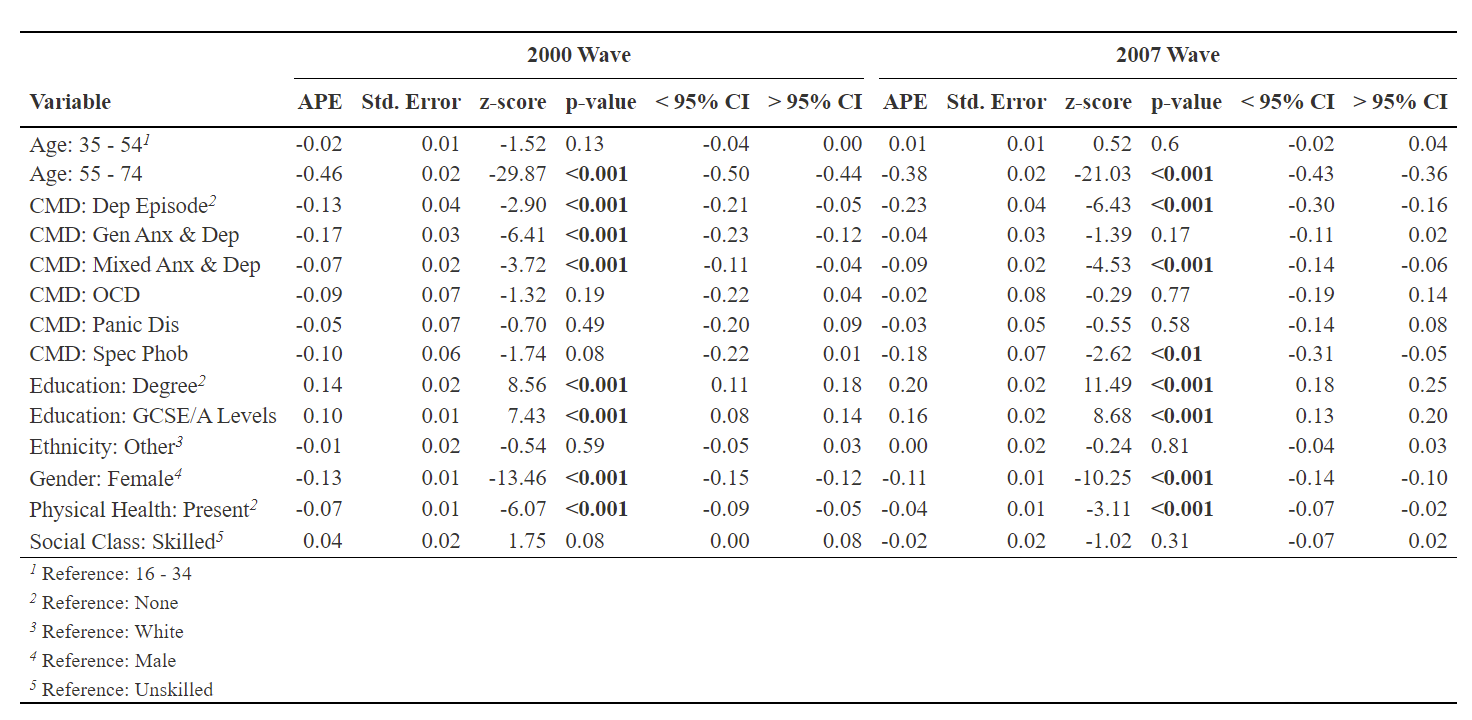
\includegraphics[width=460px,height=200px]{figure/apecmdt} \caption[Average Partial Effects for CMD Type]{Average Partial Effects for CMD Type in 2000 and 2007}\label{fig:apecmdt}
\end{figure}
With common mental health disorders type added to the model, and similar to previous sections, the largest positive effects for being economically active was having a degree or GSCE's or A Level's or their equivalent and statistically significant.

The largest negative probability associated with economic activity (apart from being aged 55 to 74) was generalised anxiety and depression in the 2000 survey (-17\%) and depression in the 2007 survey (-23\%) and were both statistically significant. This could be due to living with the conditions themselves. GAD can cause difficulty with concentration, memory, and decision-making, which can make it difficult for individuals with the disorder to perform well in a work setting. GAD can also cause physical symptoms such as fatigue, muscle tension, and sleep disturbances, which can make it difficult for people with the disorder to attend work consistently. Stigma surrounding mental illness can also be a factor as it can make it difficult for people with GAD to disclose their disorder to their employer or to seek accommodations at work, and limit access to treatment due to lack of awareness, lack of resources, or fear of stigma. Without treatment, it can be more difficult for individuals with GAD to manage their symptoms and function while being economically active.

Depression also causes difficulty in daily functioning, including trouble with concentration, motivation, and decision-making, which can make it difficult for people with the disorder to perform well in a work setting, or in other activities associated with economic activity. Depression can also cause physical symptoms such as fatigue, changes in appetite and sleep patterns, and loss of energy, which can make it difficult for people with the disorder to attend work consistently, and along with similar stigma and lack of access to treatment for some, could explain these differences.

Mixed anxiety and depression (7\% in 2000 and 9\% in 2007), OCD (9\% in 2000 and 2\% in 2007) and specific phobias (10\% in 2000 and 18\% in 2007) and panic disorder (5\% and 3\%) were all associated with decreased probability of economic activity in both survey waves. Mixed anxiety and depression were statistically significant across both survey waves, and specific phobias were significant in the 2007 wave only. OCD was not statistically significant. This could be due to changes in the rate or way that phobias are diagnosed or treated, changes in the prevalence of phobias within the population, or changes in the availability or accessibility of mental health services, and important to note that changes in the rate of diagnosis do not necessarily reflect changes in the actual prevalence of the condition, but rather may reflect changes in the way that the condition is identified and diagnosed.




\begin{figure}
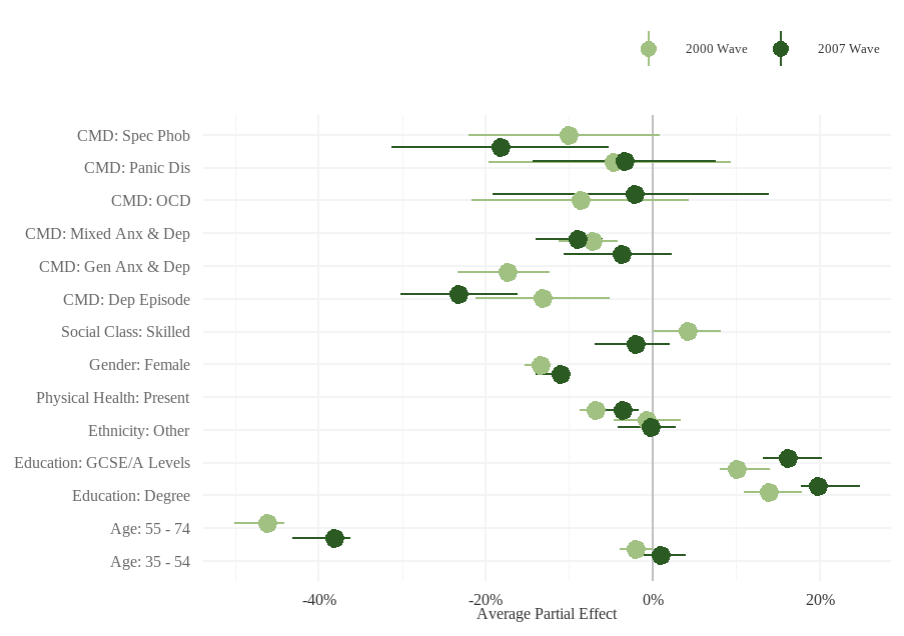
\includegraphics[width=450px,height=300px]{figure/apecmdtp} \caption[Average Partial Effects Plot of CMD Type]{Average Partial Effects Plot of CMD Type in 2000 and 2007}\label{fig:apecmdtp}
\end{figure}
\hypertarget{goodness-of-fit-for-type-of-common-mental-health-disorder}{%
\subsection{Goodness of Fit for Type of Common Mental Health Disorder}\label{goodness-of-fit-for-type-of-common-mental-health-disorder}}

Table \ref{fig:gofcmdt} presents the results of the diagnostic goodness of fit tests run on the two models examining the relationship between economic activity and common mental health disorder type in 2000 and 2007. Although the McFadden's pseudo R2 statistic ranges from 0.28 for the 2000 survey model to 0.25 for the 2007 survey model, indicating a good fit, it is worth noting that there is a slight decline in the fit of the 2007 model as compared to the 2000 model.




\begin{figure}
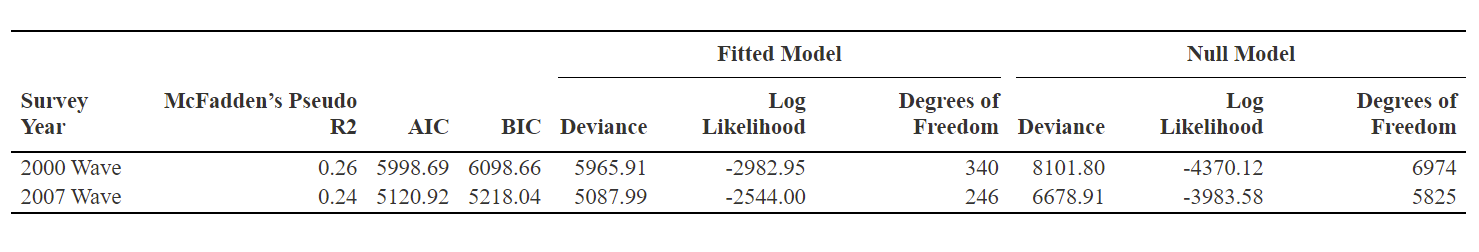
\includegraphics[width=460px,height=100px]{figure/gofcmdt} \caption[Goodness of Fit for CMD Type Models]{Goodness of Fit for CMD Type Models in 2000 and 2007}\label{fig:gofcmdt}
\end{figure}
\hypertarget{severe-mental-illness-and-economic-activity}{%
\section{Severe Mental Illness and Economic Activity}\label{severe-mental-illness-and-economic-activity}}

In this section similar to section 6.4, we explore whether the use of health services or treatments for severe mental illness might influence employment outcomes. As these are concerned with the impact of severe mental illness on economic activity, variables relating to having a severe mental illness were also added as predictors, these were having used any mental health services in the last year of the surveys being taken, and undertaking a form of mental health treatment, these being counselling, medication, or both. Mental health service or treatment use here indicates a more severe level of severe mental illness, with the parameter being having not used services or treatment. As previous research suggests that treatment use may indicate more severe levels of severe mental illness, it is important to consider whether this may have a negative impact on economic activity. As in previous sections in this chapter, logistic regression models were applied to each survey of data, two models in total for each of the survey waves.

\hypertarget{model-results-for-severe-mental-illness}{%
\subsection{Model Results for Severe Mental Illness}\label{model-results-for-severe-mental-illness}}

Table \ref{tab:results2-smimod} describes the adjusted odds ratios and significance levels for each of the models, and average partial effects are discussed in full to better understand the model results. As in previous models, the positive, statistically significant variables associated with being economically active are having a degree or GSCE or A Levels. In the 2000 survey being within the skilled social class group is also positively associated with activity but is statistically insignificant. In the 2007 survey the only other positively associated variable is being aged between 35 and 54 years old, but this is also statistically insignificant.

The adjusted odds ratios for the predictor looking at the presence of severe mental illness is negatively associated with being economically active in both of the survey waves and is also highly statistically significant. As with common mental health disorders, the effect is reduced in comparison with the model where there are no controls for MH service use or treatments, but it shows that, even for the less unwell, the probability of being economically active is greatly reduced.

\providecommand{\huxb}[2]{\arrayrulecolor[RGB]{#1}\global\arrayrulewidth=#2pt}
  \providecommand{\huxvb}[2]{\color[RGB]{#1}\vrule width #2pt}
  \providecommand{\huxtpad}[1]{\rule{0pt}{#1}}
  \providecommand{\huxbpad}[1]{\rule[-#1]{0pt}{#1}}
\begin{table}[h!]
\begin{centerbox}
\begin{threeparttable}
 \setlength{\tabcolsep}{0pt}
\begin{adjustbox}{width=1\textwidth}
\normalsize
\begin{tabular}{l l l l l l l l l}


\hhline{>{\arrayrulecolor[RGB]{0, 0, 0}\global\arrayrulewidth=0.4pt}->{\arrayrulecolor[RGB]{0, 0, 0}\global\arrayrulewidth=0.4pt}->{\arrayrulecolor[RGB]{0, 0, 0}\global\arrayrulewidth=0.4pt}->{\arrayrulecolor[RGB]{0, 0, 0}\global\arrayrulewidth=0.4pt}->{\arrayrulecolor[RGB]{0, 0, 0}\global\arrayrulewidth=0.4pt}->{\arrayrulecolor[RGB]{0, 0, 0}\global\arrayrulewidth=0.4pt}->{\arrayrulecolor[RGB]{0, 0, 0}\global\arrayrulewidth=0.4pt}->{\arrayrulecolor[RGB]{0, 0, 0}\global\arrayrulewidth=0.4pt}->{\arrayrulecolor[RGB]{0, 0, 0}\global\arrayrulewidth=0.4pt}-}
\arrayrulecolor{black}

\multicolumn{1}{!{\color[RGB]{0, 0, 0}\vrule width 0pt}l!{\color[RGB]{0, 0, 0}\vrule width 0pt}}{\rule{0pt}{1pt + 1em}\raggedright \hspace{0pt} \textbf{{\fontsize{14pt}{16.8pt}\selectfont 
}} \hspace{1pt}\rule[-1pt]{0pt}{1pt}} &
\multicolumn{4}{c!{\color[RGB]{0, 0, 0}\vrule width 0pt}}{\rule{0pt}{1pt + 1em}\centering \hspace{1pt} \textbf{{\fontsize{14pt}{16.8pt}\selectfont \textbf{2000 Wave}
}} \hspace{1pt}\rule[-1pt]{0pt}{1pt}} &
\multicolumn{4}{c!{\color[RGB]{0, 0, 0}\vrule width 0pt}}{\rule{0pt}{1pt + 1em}\centering \hspace{1pt} \textbf{{\fontsize{14pt}{16.8pt}\selectfont \textbf{2007 Wave}
}} \hspace{1pt}\rule[-1pt]{0pt}{1pt}} \tabularnewline[-0.5pt]


\hhline{}
\arrayrulecolor{black}

\multicolumn{1}{!{\color[RGB]{0, 0, 0}\vrule width 0pt}l!{\color[RGB]{0, 0, 0}\vrule width 0pt}}{\rule{0pt}{1pt + 1em}\raggedright \hspace{0pt} \textbf{{\fontsize{14pt}{16.8pt}\selectfont \textbf{Characteristic}
}} \hspace{1pt}\rule[-1pt]{0pt}{1pt}} &
\multicolumn{1}{c!{\color[RGB]{0, 0, 0}\vrule width 0pt}}{\rule{0pt}{1pt + 1em}\centering \hspace{1pt} \textbf{{\fontsize{14pt}{16.8pt}\selectfont \textbf{N}
}} \hspace{1pt}\rule[-1pt]{0pt}{1pt}} &
\multicolumn{1}{c!{\color[RGB]{0, 0, 0}\vrule width 0pt}}{\rule{0pt}{1pt + 1em}\centering \hspace{1pt} \textbf{{\fontsize{14pt}{16.8pt}\selectfont \textbf{OR}
}} \hspace{1pt}\rule[-1pt]{0pt}{1pt}} &
\multicolumn{1}{c!{\color[RGB]{0, 0, 0}\vrule width 0pt}}{\rule{0pt}{1pt + 1em}\centering \hspace{1pt} \textbf{{\fontsize{14pt}{16.8pt}\selectfont \textbf{95\% CI}
}} \hspace{1pt}\rule[-1pt]{0pt}{1pt}} &
\multicolumn{1}{c!{\color[RGB]{0, 0, 0}\vrule width 0pt}}{\rule{0pt}{1pt + 1em}\centering \hspace{1pt} \textbf{{\fontsize{14pt}{16.8pt}\selectfont \textbf{p-value}
}} \hspace{1pt}\rule[-1pt]{0pt}{1pt}} &
\multicolumn{1}{c!{\color[RGB]{0, 0, 0}\vrule width 0pt}}{\rule{0pt}{1pt + 1em}\centering \hspace{1pt} \textbf{{\fontsize{14pt}{16.8pt}\selectfont \textbf{N}
}} \hspace{1pt}\rule[-1pt]{0pt}{1pt}} &
\multicolumn{1}{c!{\color[RGB]{0, 0, 0}\vrule width 0pt}}{\rule{0pt}{1pt + 1em}\centering \hspace{1pt} \textbf{{\fontsize{14pt}{16.8pt}\selectfont \textbf{OR}
}} \hspace{1pt}\rule[-1pt]{0pt}{1pt}} &
\multicolumn{1}{c!{\color[RGB]{0, 0, 0}\vrule width 0pt}}{\rule{0pt}{1pt + 1em}\centering \hspace{1pt} \textbf{{\fontsize{14pt}{16.8pt}\selectfont \textbf{95\% CI}
}} \hspace{1pt}\rule[-1pt]{0pt}{1pt}} &
\multicolumn{1}{c!{\color[RGB]{0, 0, 0}\vrule width 0pt}}{\rule{0pt}{1pt + 1em}\centering \hspace{1pt} \textbf{{\fontsize{14pt}{16.8pt}\selectfont \textbf{p-value}
}} \hspace{0pt}\rule[-1pt]{0pt}{1pt}} \tabularnewline[-0.5pt]


\hhline{>{\arrayrulecolor[RGB]{0, 0, 0}\global\arrayrulewidth=0.4pt}->{\arrayrulecolor[RGB]{0, 0, 0}\global\arrayrulewidth=0.4pt}->{\arrayrulecolor[RGB]{0, 0, 0}\global\arrayrulewidth=0.4pt}->{\arrayrulecolor[RGB]{0, 0, 0}\global\arrayrulewidth=0.4pt}->{\arrayrulecolor[RGB]{0, 0, 0}\global\arrayrulewidth=0.4pt}->{\arrayrulecolor[RGB]{0, 0, 0}\global\arrayrulewidth=0.4pt}->{\arrayrulecolor[RGB]{0, 0, 0}\global\arrayrulewidth=0.4pt}->{\arrayrulecolor[RGB]{0, 0, 0}\global\arrayrulewidth=0.4pt}->{\arrayrulecolor[RGB]{0, 0, 0}\global\arrayrulewidth=0.4pt}-}
\arrayrulecolor{black}

\multicolumn{1}{!{\color[RGB]{0, 0, 0}\vrule width 0pt}l!{\color[RGB]{0, 0, 0}\vrule width 0pt}}{\rule{0pt}{1pt + 1em}\raggedright \hspace{0pt} \textbf{{\fontsize{14pt}{16.8pt}\selectfont Severe Mental Illness}} \hspace{1pt}\rule[-1pt]{0pt}{1pt}} &
\multicolumn{1}{c!{\color[RGB]{0, 0, 0}\vrule width 0pt}}{\rule{0pt}{1pt + 1em}\centering \hspace{1pt} {\fontsize{14pt}{16.8pt}\selectfont 6,920} \hspace{1pt}\rule[-1pt]{0pt}{1pt}} &
\multicolumn{1}{c!{\color[RGB]{0, 0, 0}\vrule width 0pt}}{\rule{0pt}{1pt + 1em}\centering \hspace{1pt} {\fontsize{14pt}{16.8pt}\selectfont } \hspace{1pt}\rule[-1pt]{0pt}{1pt}} &
\multicolumn{1}{c!{\color[RGB]{0, 0, 0}\vrule width 0pt}}{\rule{0pt}{1pt + 1em}\centering \hspace{1pt} {\fontsize{14pt}{16.8pt}\selectfont } \hspace{1pt}\rule[-1pt]{0pt}{1pt}} &
\multicolumn{1}{c!{\color[RGB]{0, 0, 0}\vrule width 0pt}}{\rule{0pt}{1pt + 1em}\centering \hspace{1pt} {\fontsize{14pt}{16.8pt}\selectfont } \hspace{1pt}\rule[-1pt]{0pt}{1pt}} &
\multicolumn{1}{c!{\color[RGB]{0, 0, 0}\vrule width 0pt}}{\rule{0pt}{1pt + 1em}\centering \hspace{1pt} {\fontsize{14pt}{16.8pt}\selectfont 5,736} \hspace{1pt}\rule[-1pt]{0pt}{1pt}} &
\multicolumn{1}{c!{\color[RGB]{0, 0, 0}\vrule width 0pt}}{\rule{0pt}{1pt + 1em}\centering \hspace{1pt} {\fontsize{14pt}{16.8pt}\selectfont } \hspace{1pt}\rule[-1pt]{0pt}{1pt}} &
\multicolumn{1}{c!{\color[RGB]{0, 0, 0}\vrule width 0pt}}{\rule{0pt}{1pt + 1em}\centering \hspace{1pt} {\fontsize{14pt}{16.8pt}\selectfont } \hspace{1pt}\rule[-1pt]{0pt}{1pt}} &
\multicolumn{1}{c!{\color[RGB]{0, 0, 0}\vrule width 0pt}}{\rule{0pt}{1pt + 1em}\centering \hspace{1pt} {\fontsize{14pt}{16.8pt}\selectfont } \hspace{0pt}\rule[-1pt]{0pt}{1pt}} \tabularnewline[-0.5pt]


\hhline{}
\arrayrulecolor{black}

\multicolumn{1}{!{\color[RGB]{0, 0, 0}\vrule width 0pt}l!{\color[RGB]{0, 0, 0}\vrule width 0pt}}{\rule{0pt}{1pt + 1em}\raggedright \hspace{0pt} {\fontsize{14pt}{16.8pt}\selectfont None} \hspace{1pt}\rule[-1pt]{0pt}{1pt}} &
\multicolumn{1}{c!{\color[RGB]{0, 0, 0}\vrule width 0pt}}{\rule{0pt}{1pt + 1em}\centering \hspace{1pt} {\fontsize{14pt}{16.8pt}\selectfont } \hspace{1pt}\rule[-1pt]{0pt}{1pt}} &
\multicolumn{1}{c!{\color[RGB]{0, 0, 0}\vrule width 0pt}}{\rule{0pt}{1pt + 1em}\centering \hspace{1pt} {\fontsize{14pt}{16.8pt}\selectfont —} \hspace{1pt}\rule[-1pt]{0pt}{1pt}} &
\multicolumn{1}{c!{\color[RGB]{0, 0, 0}\vrule width 0pt}}{\rule{0pt}{1pt + 1em}\centering \hspace{1pt} {\fontsize{14pt}{16.8pt}\selectfont —} \hspace{1pt}\rule[-1pt]{0pt}{1pt}} &
\multicolumn{1}{c!{\color[RGB]{0, 0, 0}\vrule width 0pt}}{\rule{0pt}{1pt + 1em}\centering \hspace{1pt} {\fontsize{14pt}{16.8pt}\selectfont } \hspace{1pt}\rule[-1pt]{0pt}{1pt}} &
\multicolumn{1}{c!{\color[RGB]{0, 0, 0}\vrule width 0pt}}{\rule{0pt}{1pt + 1em}\centering \hspace{1pt} {\fontsize{14pt}{16.8pt}\selectfont } \hspace{1pt}\rule[-1pt]{0pt}{1pt}} &
\multicolumn{1}{c!{\color[RGB]{0, 0, 0}\vrule width 0pt}}{\rule{0pt}{1pt + 1em}\centering \hspace{1pt} {\fontsize{14pt}{16.8pt}\selectfont —} \hspace{1pt}\rule[-1pt]{0pt}{1pt}} &
\multicolumn{1}{c!{\color[RGB]{0, 0, 0}\vrule width 0pt}}{\rule{0pt}{1pt + 1em}\centering \hspace{1pt} {\fontsize{14pt}{16.8pt}\selectfont —} \hspace{1pt}\rule[-1pt]{0pt}{1pt}} &
\multicolumn{1}{c!{\color[RGB]{0, 0, 0}\vrule width 0pt}}{\rule{0pt}{1pt + 1em}\centering \hspace{1pt} {\fontsize{14pt}{16.8pt}\selectfont } \hspace{0pt}\rule[-1pt]{0pt}{1pt}} \tabularnewline[-0.5pt]


\hhline{}
\arrayrulecolor{black}

\multicolumn{1}{!{\color[RGB]{0, 0, 0}\vrule width 0pt}l!{\color[RGB]{0, 0, 0}\vrule width 0pt}}{\rule{0pt}{1pt + 1em}\raggedright \hspace{0pt} {\fontsize{14pt}{16.8pt}\selectfont Present} \hspace{1pt}\rule[-1pt]{0pt}{1pt}} &
\multicolumn{1}{c!{\color[RGB]{0, 0, 0}\vrule width 0pt}}{\rule{0pt}{1pt + 1em}\centering \hspace{1pt} {\fontsize{14pt}{16.8pt}\selectfont } \hspace{1pt}\rule[-1pt]{0pt}{1pt}} &
\multicolumn{1}{c!{\color[RGB]{0, 0, 0}\vrule width 0pt}}{\rule{0pt}{1pt + 1em}\centering \hspace{1pt} {\fontsize{14pt}{16.8pt}\selectfont 0.48} \hspace{1pt}\rule[-1pt]{0pt}{1pt}} &
\multicolumn{1}{c!{\color[RGB]{0, 0, 0}\vrule width 0pt}}{\rule{0pt}{1pt + 1em}\centering \hspace{1pt} {\fontsize{14pt}{16.8pt}\selectfont 0.25, 0.91} \hspace{1pt}\rule[-1pt]{0pt}{1pt}} &
\multicolumn{1}{c!{\color[RGB]{0, 0, 0}\vrule width 0pt}}{\rule{0pt}{1pt + 1em}\centering \hspace{1pt} \textbf{{\fontsize{14pt}{16.8pt}\selectfont 0.024}} \hspace{1pt}\rule[-1pt]{0pt}{1pt}} &
\multicolumn{1}{c!{\color[RGB]{0, 0, 0}\vrule width 0pt}}{\rule{0pt}{1pt + 1em}\centering \hspace{1pt} {\fontsize{14pt}{16.8pt}\selectfont } \hspace{1pt}\rule[-1pt]{0pt}{1pt}} &
\multicolumn{1}{c!{\color[RGB]{0, 0, 0}\vrule width 0pt}}{\rule{0pt}{1pt + 1em}\centering \hspace{1pt} {\fontsize{14pt}{16.8pt}\selectfont 0.32} \hspace{1pt}\rule[-1pt]{0pt}{1pt}} &
\multicolumn{1}{c!{\color[RGB]{0, 0, 0}\vrule width 0pt}}{\rule{0pt}{1pt + 1em}\centering \hspace{1pt} {\fontsize{14pt}{16.8pt}\selectfont 0.16, 0.62} \hspace{1pt}\rule[-1pt]{0pt}{1pt}} &
\multicolumn{1}{c!{\color[RGB]{0, 0, 0}\vrule width 0pt}}{\rule{0pt}{1pt + 1em}\centering \hspace{1pt} \textbf{{\fontsize{14pt}{16.8pt}\selectfont $<$0.001}} \hspace{0pt}\rule[-1pt]{0pt}{1pt}} \tabularnewline[-0.5pt]


\hhline{}
\arrayrulecolor{black}

\multicolumn{1}{!{\color[RGB]{0, 0, 0}\vrule width 0pt}l!{\color[RGB]{0, 0, 0}\vrule width 0pt}}{\rule{0pt}{1pt + 1em}\raggedright \hspace{0pt} \textbf{{\fontsize{14pt}{16.8pt}\selectfont Gender}} \hspace{1pt}\rule[-1pt]{0pt}{1pt}} &
\multicolumn{1}{c!{\color[RGB]{0, 0, 0}\vrule width 0pt}}{\rule{0pt}{1pt + 1em}\centering \hspace{1pt} {\fontsize{14pt}{16.8pt}\selectfont 6,920} \hspace{1pt}\rule[-1pt]{0pt}{1pt}} &
\multicolumn{1}{c!{\color[RGB]{0, 0, 0}\vrule width 0pt}}{\rule{0pt}{1pt + 1em}\centering \hspace{1pt} {\fontsize{14pt}{16.8pt}\selectfont } \hspace{1pt}\rule[-1pt]{0pt}{1pt}} &
\multicolumn{1}{c!{\color[RGB]{0, 0, 0}\vrule width 0pt}}{\rule{0pt}{1pt + 1em}\centering \hspace{1pt} {\fontsize{14pt}{16.8pt}\selectfont } \hspace{1pt}\rule[-1pt]{0pt}{1pt}} &
\multicolumn{1}{c!{\color[RGB]{0, 0, 0}\vrule width 0pt}}{\rule{0pt}{1pt + 1em}\centering \hspace{1pt} {\fontsize{14pt}{16.8pt}\selectfont } \hspace{1pt}\rule[-1pt]{0pt}{1pt}} &
\multicolumn{1}{c!{\color[RGB]{0, 0, 0}\vrule width 0pt}}{\rule{0pt}{1pt + 1em}\centering \hspace{1pt} {\fontsize{14pt}{16.8pt}\selectfont 5,736} \hspace{1pt}\rule[-1pt]{0pt}{1pt}} &
\multicolumn{1}{c!{\color[RGB]{0, 0, 0}\vrule width 0pt}}{\rule{0pt}{1pt + 1em}\centering \hspace{1pt} {\fontsize{14pt}{16.8pt}\selectfont } \hspace{1pt}\rule[-1pt]{0pt}{1pt}} &
\multicolumn{1}{c!{\color[RGB]{0, 0, 0}\vrule width 0pt}}{\rule{0pt}{1pt + 1em}\centering \hspace{1pt} {\fontsize{14pt}{16.8pt}\selectfont } \hspace{1pt}\rule[-1pt]{0pt}{1pt}} &
\multicolumn{1}{c!{\color[RGB]{0, 0, 0}\vrule width 0pt}}{\rule{0pt}{1pt + 1em}\centering \hspace{1pt} {\fontsize{14pt}{16.8pt}\selectfont } \hspace{0pt}\rule[-1pt]{0pt}{1pt}} \tabularnewline[-0.5pt]


\hhline{}
\arrayrulecolor{black}

\multicolumn{1}{!{\color[RGB]{0, 0, 0}\vrule width 0pt}l!{\color[RGB]{0, 0, 0}\vrule width 0pt}}{\rule{0pt}{1pt + 1em}\raggedright \hspace{0pt} {\fontsize{14pt}{16.8pt}\selectfont Male} \hspace{1pt}\rule[-1pt]{0pt}{1pt}} &
\multicolumn{1}{c!{\color[RGB]{0, 0, 0}\vrule width 0pt}}{\rule{0pt}{1pt + 1em}\centering \hspace{1pt} {\fontsize{14pt}{16.8pt}\selectfont } \hspace{1pt}\rule[-1pt]{0pt}{1pt}} &
\multicolumn{1}{c!{\color[RGB]{0, 0, 0}\vrule width 0pt}}{\rule{0pt}{1pt + 1em}\centering \hspace{1pt} {\fontsize{14pt}{16.8pt}\selectfont —} \hspace{1pt}\rule[-1pt]{0pt}{1pt}} &
\multicolumn{1}{c!{\color[RGB]{0, 0, 0}\vrule width 0pt}}{\rule{0pt}{1pt + 1em}\centering \hspace{1pt} {\fontsize{14pt}{16.8pt}\selectfont —} \hspace{1pt}\rule[-1pt]{0pt}{1pt}} &
\multicolumn{1}{c!{\color[RGB]{0, 0, 0}\vrule width 0pt}}{\rule{0pt}{1pt + 1em}\centering \hspace{1pt} {\fontsize{14pt}{16.8pt}\selectfont } \hspace{1pt}\rule[-1pt]{0pt}{1pt}} &
\multicolumn{1}{c!{\color[RGB]{0, 0, 0}\vrule width 0pt}}{\rule{0pt}{1pt + 1em}\centering \hspace{1pt} {\fontsize{14pt}{16.8pt}\selectfont } \hspace{1pt}\rule[-1pt]{0pt}{1pt}} &
\multicolumn{1}{c!{\color[RGB]{0, 0, 0}\vrule width 0pt}}{\rule{0pt}{1pt + 1em}\centering \hspace{1pt} {\fontsize{14pt}{16.8pt}\selectfont —} \hspace{1pt}\rule[-1pt]{0pt}{1pt}} &
\multicolumn{1}{c!{\color[RGB]{0, 0, 0}\vrule width 0pt}}{\rule{0pt}{1pt + 1em}\centering \hspace{1pt} {\fontsize{14pt}{16.8pt}\selectfont —} \hspace{1pt}\rule[-1pt]{0pt}{1pt}} &
\multicolumn{1}{c!{\color[RGB]{0, 0, 0}\vrule width 0pt}}{\rule{0pt}{1pt + 1em}\centering \hspace{1pt} {\fontsize{14pt}{16.8pt}\selectfont } \hspace{0pt}\rule[-1pt]{0pt}{1pt}} \tabularnewline[-0.5pt]


\hhline{}
\arrayrulecolor{black}

\multicolumn{1}{!{\color[RGB]{0, 0, 0}\vrule width 0pt}l!{\color[RGB]{0, 0, 0}\vrule width 0pt}}{\rule{0pt}{1pt + 1em}\raggedright \hspace{0pt} {\fontsize{14pt}{16.8pt}\selectfont Female} \hspace{1pt}\rule[-1pt]{0pt}{1pt}} &
\multicolumn{1}{c!{\color[RGB]{0, 0, 0}\vrule width 0pt}}{\rule{0pt}{1pt + 1em}\centering \hspace{1pt} {\fontsize{14pt}{16.8pt}\selectfont } \hspace{1pt}\rule[-1pt]{0pt}{1pt}} &
\multicolumn{1}{c!{\color[RGB]{0, 0, 0}\vrule width 0pt}}{\rule{0pt}{1pt + 1em}\centering \hspace{1pt} {\fontsize{14pt}{16.8pt}\selectfont 0.40} \hspace{1pt}\rule[-1pt]{0pt}{1pt}} &
\multicolumn{1}{c!{\color[RGB]{0, 0, 0}\vrule width 0pt}}{\rule{0pt}{1pt + 1em}\centering \hspace{1pt} {\fontsize{14pt}{16.8pt}\selectfont 0.35, 0.46} \hspace{1pt}\rule[-1pt]{0pt}{1pt}} &
\multicolumn{1}{c!{\color[RGB]{0, 0, 0}\vrule width 0pt}}{\rule{0pt}{1pt + 1em}\centering \hspace{1pt} \textbf{{\fontsize{14pt}{16.8pt}\selectfont $<$0.001}} \hspace{1pt}\rule[-1pt]{0pt}{1pt}} &
\multicolumn{1}{c!{\color[RGB]{0, 0, 0}\vrule width 0pt}}{\rule{0pt}{1pt + 1em}\centering \hspace{1pt} {\fontsize{14pt}{16.8pt}\selectfont } \hspace{1pt}\rule[-1pt]{0pt}{1pt}} &
\multicolumn{1}{c!{\color[RGB]{0, 0, 0}\vrule width 0pt}}{\rule{0pt}{1pt + 1em}\centering \hspace{1pt} {\fontsize{14pt}{16.8pt}\selectfont 0.46} \hspace{1pt}\rule[-1pt]{0pt}{1pt}} &
\multicolumn{1}{c!{\color[RGB]{0, 0, 0}\vrule width 0pt}}{\rule{0pt}{1pt + 1em}\centering \hspace{1pt} {\fontsize{14pt}{16.8pt}\selectfont 0.40, 0.53} \hspace{1pt}\rule[-1pt]{0pt}{1pt}} &
\multicolumn{1}{c!{\color[RGB]{0, 0, 0}\vrule width 0pt}}{\rule{0pt}{1pt + 1em}\centering \hspace{1pt} \textbf{{\fontsize{14pt}{16.8pt}\selectfont $<$0.001}} \hspace{0pt}\rule[-1pt]{0pt}{1pt}} \tabularnewline[-0.5pt]


\hhline{}
\arrayrulecolor{black}

\multicolumn{1}{!{\color[RGB]{0, 0, 0}\vrule width 0pt}l!{\color[RGB]{0, 0, 0}\vrule width 0pt}}{\rule{0pt}{1pt + 1em}\raggedright \hspace{0pt} \textbf{{\fontsize{14pt}{16.8pt}\selectfont Age Band}} \hspace{1pt}\rule[-1pt]{0pt}{1pt}} &
\multicolumn{1}{c!{\color[RGB]{0, 0, 0}\vrule width 0pt}}{\rule{0pt}{1pt + 1em}\centering \hspace{1pt} {\fontsize{14pt}{16.8pt}\selectfont 6,920} \hspace{1pt}\rule[-1pt]{0pt}{1pt}} &
\multicolumn{1}{c!{\color[RGB]{0, 0, 0}\vrule width 0pt}}{\rule{0pt}{1pt + 1em}\centering \hspace{1pt} {\fontsize{14pt}{16.8pt}\selectfont } \hspace{1pt}\rule[-1pt]{0pt}{1pt}} &
\multicolumn{1}{c!{\color[RGB]{0, 0, 0}\vrule width 0pt}}{\rule{0pt}{1pt + 1em}\centering \hspace{1pt} {\fontsize{14pt}{16.8pt}\selectfont } \hspace{1pt}\rule[-1pt]{0pt}{1pt}} &
\multicolumn{1}{c!{\color[RGB]{0, 0, 0}\vrule width 0pt}}{\rule{0pt}{1pt + 1em}\centering \hspace{1pt} {\fontsize{14pt}{16.8pt}\selectfont } \hspace{1pt}\rule[-1pt]{0pt}{1pt}} &
\multicolumn{1}{c!{\color[RGB]{0, 0, 0}\vrule width 0pt}}{\rule{0pt}{1pt + 1em}\centering \hspace{1pt} {\fontsize{14pt}{16.8pt}\selectfont 5,736} \hspace{1pt}\rule[-1pt]{0pt}{1pt}} &
\multicolumn{1}{c!{\color[RGB]{0, 0, 0}\vrule width 0pt}}{\rule{0pt}{1pt + 1em}\centering \hspace{1pt} {\fontsize{14pt}{16.8pt}\selectfont } \hspace{1pt}\rule[-1pt]{0pt}{1pt}} &
\multicolumn{1}{c!{\color[RGB]{0, 0, 0}\vrule width 0pt}}{\rule{0pt}{1pt + 1em}\centering \hspace{1pt} {\fontsize{14pt}{16.8pt}\selectfont } \hspace{1pt}\rule[-1pt]{0pt}{1pt}} &
\multicolumn{1}{c!{\color[RGB]{0, 0, 0}\vrule width 0pt}}{\rule{0pt}{1pt + 1em}\centering \hspace{1pt} {\fontsize{14pt}{16.8pt}\selectfont } \hspace{0pt}\rule[-1pt]{0pt}{1pt}} \tabularnewline[-0.5pt]


\hhline{}
\arrayrulecolor{black}

\multicolumn{1}{!{\color[RGB]{0, 0, 0}\vrule width 0pt}l!{\color[RGB]{0, 0, 0}\vrule width 0pt}}{\rule{0pt}{1pt + 1em}\raggedright \hspace{0pt} {\fontsize{14pt}{16.8pt}\selectfont 16 - 34} \hspace{1pt}\rule[-1pt]{0pt}{1pt}} &
\multicolumn{1}{c!{\color[RGB]{0, 0, 0}\vrule width 0pt}}{\rule{0pt}{1pt + 1em}\centering \hspace{1pt} {\fontsize{14pt}{16.8pt}\selectfont } \hspace{1pt}\rule[-1pt]{0pt}{1pt}} &
\multicolumn{1}{c!{\color[RGB]{0, 0, 0}\vrule width 0pt}}{\rule{0pt}{1pt + 1em}\centering \hspace{1pt} {\fontsize{14pt}{16.8pt}\selectfont —} \hspace{1pt}\rule[-1pt]{0pt}{1pt}} &
\multicolumn{1}{c!{\color[RGB]{0, 0, 0}\vrule width 0pt}}{\rule{0pt}{1pt + 1em}\centering \hspace{1pt} {\fontsize{14pt}{16.8pt}\selectfont —} \hspace{1pt}\rule[-1pt]{0pt}{1pt}} &
\multicolumn{1}{c!{\color[RGB]{0, 0, 0}\vrule width 0pt}}{\rule{0pt}{1pt + 1em}\centering \hspace{1pt} {\fontsize{14pt}{16.8pt}\selectfont } \hspace{1pt}\rule[-1pt]{0pt}{1pt}} &
\multicolumn{1}{c!{\color[RGB]{0, 0, 0}\vrule width 0pt}}{\rule{0pt}{1pt + 1em}\centering \hspace{1pt} {\fontsize{14pt}{16.8pt}\selectfont } \hspace{1pt}\rule[-1pt]{0pt}{1pt}} &
\multicolumn{1}{c!{\color[RGB]{0, 0, 0}\vrule width 0pt}}{\rule{0pt}{1pt + 1em}\centering \hspace{1pt} {\fontsize{14pt}{16.8pt}\selectfont —} \hspace{1pt}\rule[-1pt]{0pt}{1pt}} &
\multicolumn{1}{c!{\color[RGB]{0, 0, 0}\vrule width 0pt}}{\rule{0pt}{1pt + 1em}\centering \hspace{1pt} {\fontsize{14pt}{16.8pt}\selectfont —} \hspace{1pt}\rule[-1pt]{0pt}{1pt}} &
\multicolumn{1}{c!{\color[RGB]{0, 0, 0}\vrule width 0pt}}{\rule{0pt}{1pt + 1em}\centering \hspace{1pt} {\fontsize{14pt}{16.8pt}\selectfont } \hspace{0pt}\rule[-1pt]{0pt}{1pt}} \tabularnewline[-0.5pt]


\hhline{}
\arrayrulecolor{black}

\multicolumn{1}{!{\color[RGB]{0, 0, 0}\vrule width 0pt}l!{\color[RGB]{0, 0, 0}\vrule width 0pt}}{\rule{0pt}{1pt + 1em}\raggedright \hspace{0pt} {\fontsize{14pt}{16.8pt}\selectfont 35 - 54} \hspace{1pt}\rule[-1pt]{0pt}{1pt}} &
\multicolumn{1}{c!{\color[RGB]{0, 0, 0}\vrule width 0pt}}{\rule{0pt}{1pt + 1em}\centering \hspace{1pt} {\fontsize{14pt}{16.8pt}\selectfont } \hspace{1pt}\rule[-1pt]{0pt}{1pt}} &
\multicolumn{1}{c!{\color[RGB]{0, 0, 0}\vrule width 0pt}}{\rule{0pt}{1pt + 1em}\centering \hspace{1pt} {\fontsize{14pt}{16.8pt}\selectfont 0.92} \hspace{1pt}\rule[-1pt]{0pt}{1pt}} &
\multicolumn{1}{c!{\color[RGB]{0, 0, 0}\vrule width 0pt}}{\rule{0pt}{1pt + 1em}\centering \hspace{1pt} {\fontsize{14pt}{16.8pt}\selectfont 0.78, 1.10} \hspace{1pt}\rule[-1pt]{0pt}{1pt}} &
\multicolumn{1}{c!{\color[RGB]{0, 0, 0}\vrule width 0pt}}{\rule{0pt}{1pt + 1em}\centering \hspace{1pt} {\fontsize{14pt}{16.8pt}\selectfont 0.37} \hspace{1pt}\rule[-1pt]{0pt}{1pt}} &
\multicolumn{1}{c!{\color[RGB]{0, 0, 0}\vrule width 0pt}}{\rule{0pt}{1pt + 1em}\centering \hspace{1pt} {\fontsize{14pt}{16.8pt}\selectfont } \hspace{1pt}\rule[-1pt]{0pt}{1pt}} &
\multicolumn{1}{c!{\color[RGB]{0, 0, 0}\vrule width 0pt}}{\rule{0pt}{1pt + 1em}\centering \hspace{1pt} {\fontsize{14pt}{16.8pt}\selectfont 1.10} \hspace{1pt}\rule[-1pt]{0pt}{1pt}} &
\multicolumn{1}{c!{\color[RGB]{0, 0, 0}\vrule width 0pt}}{\rule{0pt}{1pt + 1em}\centering \hspace{1pt} {\fontsize{14pt}{16.8pt}\selectfont 0.88, 1.39} \hspace{1pt}\rule[-1pt]{0pt}{1pt}} &
\multicolumn{1}{c!{\color[RGB]{0, 0, 0}\vrule width 0pt}}{\rule{0pt}{1pt + 1em}\centering \hspace{1pt} {\fontsize{14pt}{16.8pt}\selectfont 0.40} \hspace{0pt}\rule[-1pt]{0pt}{1pt}} \tabularnewline[-0.5pt]


\hhline{}
\arrayrulecolor{black}

\multicolumn{1}{!{\color[RGB]{0, 0, 0}\vrule width 0pt}l!{\color[RGB]{0, 0, 0}\vrule width 0pt}}{\rule{0pt}{1pt + 1em}\raggedright \hspace{0pt} {\fontsize{14pt}{16.8pt}\selectfont 55 - 74} \hspace{1pt}\rule[-1pt]{0pt}{1pt}} &
\multicolumn{1}{c!{\color[RGB]{0, 0, 0}\vrule width 0pt}}{\rule{0pt}{1pt + 1em}\centering \hspace{1pt} {\fontsize{14pt}{16.8pt}\selectfont } \hspace{1pt}\rule[-1pt]{0pt}{1pt}} &
\multicolumn{1}{c!{\color[RGB]{0, 0, 0}\vrule width 0pt}}{\rule{0pt}{1pt + 1em}\centering \hspace{1pt} {\fontsize{14pt}{16.8pt}\selectfont 0.09} \hspace{1pt}\rule[-1pt]{0pt}{1pt}} &
\multicolumn{1}{c!{\color[RGB]{0, 0, 0}\vrule width 0pt}}{\rule{0pt}{1pt + 1em}\centering \hspace{1pt} {\fontsize{14pt}{16.8pt}\selectfont 0.07, 0.10} \hspace{1pt}\rule[-1pt]{0pt}{1pt}} &
\multicolumn{1}{c!{\color[RGB]{0, 0, 0}\vrule width 0pt}}{\rule{0pt}{1pt + 1em}\centering \hspace{1pt} \textbf{{\fontsize{14pt}{16.8pt}\selectfont $<$0.001}} \hspace{1pt}\rule[-1pt]{0pt}{1pt}} &
\multicolumn{1}{c!{\color[RGB]{0, 0, 0}\vrule width 0pt}}{\rule{0pt}{1pt + 1em}\centering \hspace{1pt} {\fontsize{14pt}{16.8pt}\selectfont } \hspace{1pt}\rule[-1pt]{0pt}{1pt}} &
\multicolumn{1}{c!{\color[RGB]{0, 0, 0}\vrule width 0pt}}{\rule{0pt}{1pt + 1em}\centering \hspace{1pt} {\fontsize{14pt}{16.8pt}\selectfont 0.13} \hspace{1pt}\rule[-1pt]{0pt}{1pt}} &
\multicolumn{1}{c!{\color[RGB]{0, 0, 0}\vrule width 0pt}}{\rule{0pt}{1pt + 1em}\centering \hspace{1pt} {\fontsize{14pt}{16.8pt}\selectfont 0.11, 0.17} \hspace{1pt}\rule[-1pt]{0pt}{1pt}} &
\multicolumn{1}{c!{\color[RGB]{0, 0, 0}\vrule width 0pt}}{\rule{0pt}{1pt + 1em}\centering \hspace{1pt} \textbf{{\fontsize{14pt}{16.8pt}\selectfont $<$0.001}} \hspace{0pt}\rule[-1pt]{0pt}{1pt}} \tabularnewline[-0.5pt]


\hhline{}
\arrayrulecolor{black}

\multicolumn{1}{!{\color[RGB]{0, 0, 0}\vrule width 0pt}l!{\color[RGB]{0, 0, 0}\vrule width 0pt}}{\rule{0pt}{1pt + 1em}\raggedright \hspace{0pt} \textbf{{\fontsize{14pt}{16.8pt}\selectfont Ethnicity}} \hspace{1pt}\rule[-1pt]{0pt}{1pt}} &
\multicolumn{1}{c!{\color[RGB]{0, 0, 0}\vrule width 0pt}}{\rule{0pt}{1pt + 1em}\centering \hspace{1pt} {\fontsize{14pt}{16.8pt}\selectfont 6,920} \hspace{1pt}\rule[-1pt]{0pt}{1pt}} &
\multicolumn{1}{c!{\color[RGB]{0, 0, 0}\vrule width 0pt}}{\rule{0pt}{1pt + 1em}\centering \hspace{1pt} {\fontsize{14pt}{16.8pt}\selectfont } \hspace{1pt}\rule[-1pt]{0pt}{1pt}} &
\multicolumn{1}{c!{\color[RGB]{0, 0, 0}\vrule width 0pt}}{\rule{0pt}{1pt + 1em}\centering \hspace{1pt} {\fontsize{14pt}{16.8pt}\selectfont } \hspace{1pt}\rule[-1pt]{0pt}{1pt}} &
\multicolumn{1}{c!{\color[RGB]{0, 0, 0}\vrule width 0pt}}{\rule{0pt}{1pt + 1em}\centering \hspace{1pt} {\fontsize{14pt}{16.8pt}\selectfont } \hspace{1pt}\rule[-1pt]{0pt}{1pt}} &
\multicolumn{1}{c!{\color[RGB]{0, 0, 0}\vrule width 0pt}}{\rule{0pt}{1pt + 1em}\centering \hspace{1pt} {\fontsize{14pt}{16.8pt}\selectfont 5,736} \hspace{1pt}\rule[-1pt]{0pt}{1pt}} &
\multicolumn{1}{c!{\color[RGB]{0, 0, 0}\vrule width 0pt}}{\rule{0pt}{1pt + 1em}\centering \hspace{1pt} {\fontsize{14pt}{16.8pt}\selectfont } \hspace{1pt}\rule[-1pt]{0pt}{1pt}} &
\multicolumn{1}{c!{\color[RGB]{0, 0, 0}\vrule width 0pt}}{\rule{0pt}{1pt + 1em}\centering \hspace{1pt} {\fontsize{14pt}{16.8pt}\selectfont } \hspace{1pt}\rule[-1pt]{0pt}{1pt}} &
\multicolumn{1}{c!{\color[RGB]{0, 0, 0}\vrule width 0pt}}{\rule{0pt}{1pt + 1em}\centering \hspace{1pt} {\fontsize{14pt}{16.8pt}\selectfont } \hspace{0pt}\rule[-1pt]{0pt}{1pt}} \tabularnewline[-0.5pt]


\hhline{}
\arrayrulecolor{black}

\multicolumn{1}{!{\color[RGB]{0, 0, 0}\vrule width 0pt}l!{\color[RGB]{0, 0, 0}\vrule width 0pt}}{\rule{0pt}{1pt + 1em}\raggedright \hspace{0pt} {\fontsize{14pt}{16.8pt}\selectfont White} \hspace{1pt}\rule[-1pt]{0pt}{1pt}} &
\multicolumn{1}{c!{\color[RGB]{0, 0, 0}\vrule width 0pt}}{\rule{0pt}{1pt + 1em}\centering \hspace{1pt} {\fontsize{14pt}{16.8pt}\selectfont } \hspace{1pt}\rule[-1pt]{0pt}{1pt}} &
\multicolumn{1}{c!{\color[RGB]{0, 0, 0}\vrule width 0pt}}{\rule{0pt}{1pt + 1em}\centering \hspace{1pt} {\fontsize{14pt}{16.8pt}\selectfont —} \hspace{1pt}\rule[-1pt]{0pt}{1pt}} &
\multicolumn{1}{c!{\color[RGB]{0, 0, 0}\vrule width 0pt}}{\rule{0pt}{1pt + 1em}\centering \hspace{1pt} {\fontsize{14pt}{16.8pt}\selectfont —} \hspace{1pt}\rule[-1pt]{0pt}{1pt}} &
\multicolumn{1}{c!{\color[RGB]{0, 0, 0}\vrule width 0pt}}{\rule{0pt}{1pt + 1em}\centering \hspace{1pt} {\fontsize{14pt}{16.8pt}\selectfont } \hspace{1pt}\rule[-1pt]{0pt}{1pt}} &
\multicolumn{1}{c!{\color[RGB]{0, 0, 0}\vrule width 0pt}}{\rule{0pt}{1pt + 1em}\centering \hspace{1pt} {\fontsize{14pt}{16.8pt}\selectfont } \hspace{1pt}\rule[-1pt]{0pt}{1pt}} &
\multicolumn{1}{c!{\color[RGB]{0, 0, 0}\vrule width 0pt}}{\rule{0pt}{1pt + 1em}\centering \hspace{1pt} {\fontsize{14pt}{16.8pt}\selectfont —} \hspace{1pt}\rule[-1pt]{0pt}{1pt}} &
\multicolumn{1}{c!{\color[RGB]{0, 0, 0}\vrule width 0pt}}{\rule{0pt}{1pt + 1em}\centering \hspace{1pt} {\fontsize{14pt}{16.8pt}\selectfont —} \hspace{1pt}\rule[-1pt]{0pt}{1pt}} &
\multicolumn{1}{c!{\color[RGB]{0, 0, 0}\vrule width 0pt}}{\rule{0pt}{1pt + 1em}\centering \hspace{1pt} {\fontsize{14pt}{16.8pt}\selectfont } \hspace{0pt}\rule[-1pt]{0pt}{1pt}} \tabularnewline[-0.5pt]


\hhline{}
\arrayrulecolor{black}

\multicolumn{1}{!{\color[RGB]{0, 0, 0}\vrule width 0pt}l!{\color[RGB]{0, 0, 0}\vrule width 0pt}}{\rule{0pt}{1pt + 1em}\raggedright \hspace{0pt} {\fontsize{14pt}{16.8pt}\selectfont Other} \hspace{1pt}\rule[-1pt]{0pt}{1pt}} &
\multicolumn{1}{c!{\color[RGB]{0, 0, 0}\vrule width 0pt}}{\rule{0pt}{1pt + 1em}\centering \hspace{1pt} {\fontsize{14pt}{16.8pt}\selectfont } \hspace{1pt}\rule[-1pt]{0pt}{1pt}} &
\multicolumn{1}{c!{\color[RGB]{0, 0, 0}\vrule width 0pt}}{\rule{0pt}{1pt + 1em}\centering \hspace{1pt} {\fontsize{14pt}{16.8pt}\selectfont 0.85} \hspace{1pt}\rule[-1pt]{0pt}{1pt}} &
\multicolumn{1}{c!{\color[RGB]{0, 0, 0}\vrule width 0pt}}{\rule{0pt}{1pt + 1em}\centering \hspace{1pt} {\fontsize{14pt}{16.8pt}\selectfont 0.63, 1.15} \hspace{1pt}\rule[-1pt]{0pt}{1pt}} &
\multicolumn{1}{c!{\color[RGB]{0, 0, 0}\vrule width 0pt}}{\rule{0pt}{1pt + 1em}\centering \hspace{1pt} {\fontsize{14pt}{16.8pt}\selectfont 0.30} \hspace{1pt}\rule[-1pt]{0pt}{1pt}} &
\multicolumn{1}{c!{\color[RGB]{0, 0, 0}\vrule width 0pt}}{\rule{0pt}{1pt + 1em}\centering \hspace{1pt} {\fontsize{14pt}{16.8pt}\selectfont } \hspace{1pt}\rule[-1pt]{0pt}{1pt}} &
\multicolumn{1}{c!{\color[RGB]{0, 0, 0}\vrule width 0pt}}{\rule{0pt}{1pt + 1em}\centering \hspace{1pt} {\fontsize{14pt}{16.8pt}\selectfont 0.91} \hspace{1pt}\rule[-1pt]{0pt}{1pt}} &
\multicolumn{1}{c!{\color[RGB]{0, 0, 0}\vrule width 0pt}}{\rule{0pt}{1pt + 1em}\centering \hspace{1pt} {\fontsize{14pt}{16.8pt}\selectfont 0.70, 1.18} \hspace{1pt}\rule[-1pt]{0pt}{1pt}} &
\multicolumn{1}{c!{\color[RGB]{0, 0, 0}\vrule width 0pt}}{\rule{0pt}{1pt + 1em}\centering \hspace{1pt} {\fontsize{14pt}{16.8pt}\selectfont 0.47} \hspace{0pt}\rule[-1pt]{0pt}{1pt}} \tabularnewline[-0.5pt]


\hhline{}
\arrayrulecolor{black}

\multicolumn{1}{!{\color[RGB]{0, 0, 0}\vrule width 0pt}l!{\color[RGB]{0, 0, 0}\vrule width 0pt}}{\rule{0pt}{1pt + 1em}\raggedright \hspace{0pt} \textbf{{\fontsize{14pt}{16.8pt}\selectfont Social Class}} \hspace{1pt}\rule[-1pt]{0pt}{1pt}} &
\multicolumn{1}{c!{\color[RGB]{0, 0, 0}\vrule width 0pt}}{\rule{0pt}{1pt + 1em}\centering \hspace{1pt} {\fontsize{14pt}{16.8pt}\selectfont 6,920} \hspace{1pt}\rule[-1pt]{0pt}{1pt}} &
\multicolumn{1}{c!{\color[RGB]{0, 0, 0}\vrule width 0pt}}{\rule{0pt}{1pt + 1em}\centering \hspace{1pt} {\fontsize{14pt}{16.8pt}\selectfont } \hspace{1pt}\rule[-1pt]{0pt}{1pt}} &
\multicolumn{1}{c!{\color[RGB]{0, 0, 0}\vrule width 0pt}}{\rule{0pt}{1pt + 1em}\centering \hspace{1pt} {\fontsize{14pt}{16.8pt}\selectfont } \hspace{1pt}\rule[-1pt]{0pt}{1pt}} &
\multicolumn{1}{c!{\color[RGB]{0, 0, 0}\vrule width 0pt}}{\rule{0pt}{1pt + 1em}\centering \hspace{1pt} {\fontsize{14pt}{16.8pt}\selectfont } \hspace{1pt}\rule[-1pt]{0pt}{1pt}} &
\multicolumn{1}{c!{\color[RGB]{0, 0, 0}\vrule width 0pt}}{\rule{0pt}{1pt + 1em}\centering \hspace{1pt} {\fontsize{14pt}{16.8pt}\selectfont 5,736} \hspace{1pt}\rule[-1pt]{0pt}{1pt}} &
\multicolumn{1}{c!{\color[RGB]{0, 0, 0}\vrule width 0pt}}{\rule{0pt}{1pt + 1em}\centering \hspace{1pt} {\fontsize{14pt}{16.8pt}\selectfont } \hspace{1pt}\rule[-1pt]{0pt}{1pt}} &
\multicolumn{1}{c!{\color[RGB]{0, 0, 0}\vrule width 0pt}}{\rule{0pt}{1pt + 1em}\centering \hspace{1pt} {\fontsize{14pt}{16.8pt}\selectfont } \hspace{1pt}\rule[-1pt]{0pt}{1pt}} &
\multicolumn{1}{c!{\color[RGB]{0, 0, 0}\vrule width 0pt}}{\rule{0pt}{1pt + 1em}\centering \hspace{1pt} {\fontsize{14pt}{16.8pt}\selectfont } \hspace{0pt}\rule[-1pt]{0pt}{1pt}} \tabularnewline[-0.5pt]


\hhline{}
\arrayrulecolor{black}

\multicolumn{1}{!{\color[RGB]{0, 0, 0}\vrule width 0pt}l!{\color[RGB]{0, 0, 0}\vrule width 0pt}}{\rule{0pt}{1pt + 1em}\raggedright \hspace{0pt} {\fontsize{14pt}{16.8pt}\selectfont Unskilled} \hspace{1pt}\rule[-1pt]{0pt}{1pt}} &
\multicolumn{1}{c!{\color[RGB]{0, 0, 0}\vrule width 0pt}}{\rule{0pt}{1pt + 1em}\centering \hspace{1pt} {\fontsize{14pt}{16.8pt}\selectfont } \hspace{1pt}\rule[-1pt]{0pt}{1pt}} &
\multicolumn{1}{c!{\color[RGB]{0, 0, 0}\vrule width 0pt}}{\rule{0pt}{1pt + 1em}\centering \hspace{1pt} {\fontsize{14pt}{16.8pt}\selectfont —} \hspace{1pt}\rule[-1pt]{0pt}{1pt}} &
\multicolumn{1}{c!{\color[RGB]{0, 0, 0}\vrule width 0pt}}{\rule{0pt}{1pt + 1em}\centering \hspace{1pt} {\fontsize{14pt}{16.8pt}\selectfont —} \hspace{1pt}\rule[-1pt]{0pt}{1pt}} &
\multicolumn{1}{c!{\color[RGB]{0, 0, 0}\vrule width 0pt}}{\rule{0pt}{1pt + 1em}\centering \hspace{1pt} {\fontsize{14pt}{16.8pt}\selectfont } \hspace{1pt}\rule[-1pt]{0pt}{1pt}} &
\multicolumn{1}{c!{\color[RGB]{0, 0, 0}\vrule width 0pt}}{\rule{0pt}{1pt + 1em}\centering \hspace{1pt} {\fontsize{14pt}{16.8pt}\selectfont } \hspace{1pt}\rule[-1pt]{0pt}{1pt}} &
\multicolumn{1}{c!{\color[RGB]{0, 0, 0}\vrule width 0pt}}{\rule{0pt}{1pt + 1em}\centering \hspace{1pt} {\fontsize{14pt}{16.8pt}\selectfont —} \hspace{1pt}\rule[-1pt]{0pt}{1pt}} &
\multicolumn{1}{c!{\color[RGB]{0, 0, 0}\vrule width 0pt}}{\rule{0pt}{1pt + 1em}\centering \hspace{1pt} {\fontsize{14pt}{16.8pt}\selectfont —} \hspace{1pt}\rule[-1pt]{0pt}{1pt}} &
\multicolumn{1}{c!{\color[RGB]{0, 0, 0}\vrule width 0pt}}{\rule{0pt}{1pt + 1em}\centering \hspace{1pt} {\fontsize{14pt}{16.8pt}\selectfont } \hspace{0pt}\rule[-1pt]{0pt}{1pt}} \tabularnewline[-0.5pt]


\hhline{}
\arrayrulecolor{black}

\multicolumn{1}{!{\color[RGB]{0, 0, 0}\vrule width 0pt}l!{\color[RGB]{0, 0, 0}\vrule width 0pt}}{\rule{0pt}{1pt + 1em}\raggedright \hspace{0pt} {\fontsize{14pt}{16.8pt}\selectfont Skilled} \hspace{1pt}\rule[-1pt]{0pt}{1pt}} &
\multicolumn{1}{c!{\color[RGB]{0, 0, 0}\vrule width 0pt}}{\rule{0pt}{1pt + 1em}\centering \hspace{1pt} {\fontsize{14pt}{16.8pt}\selectfont } \hspace{1pt}\rule[-1pt]{0pt}{1pt}} &
\multicolumn{1}{c!{\color[RGB]{0, 0, 0}\vrule width 0pt}}{\rule{0pt}{1pt + 1em}\centering \hspace{1pt} {\fontsize{14pt}{16.8pt}\selectfont 1.30} \hspace{1pt}\rule[-1pt]{0pt}{1pt}} &
\multicolumn{1}{c!{\color[RGB]{0, 0, 0}\vrule width 0pt}}{\rule{0pt}{1pt + 1em}\centering \hspace{1pt} {\fontsize{14pt}{16.8pt}\selectfont 0.96, 1.76} \hspace{1pt}\rule[-1pt]{0pt}{1pt}} &
\multicolumn{1}{c!{\color[RGB]{0, 0, 0}\vrule width 0pt}}{\rule{0pt}{1pt + 1em}\centering \hspace{1pt} {\fontsize{14pt}{16.8pt}\selectfont 0.093} \hspace{1pt}\rule[-1pt]{0pt}{1pt}} &
\multicolumn{1}{c!{\color[RGB]{0, 0, 0}\vrule width 0pt}}{\rule{0pt}{1pt + 1em}\centering \hspace{1pt} {\fontsize{14pt}{16.8pt}\selectfont } \hspace{1pt}\rule[-1pt]{0pt}{1pt}} &
\multicolumn{1}{c!{\color[RGB]{0, 0, 0}\vrule width 0pt}}{\rule{0pt}{1pt + 1em}\centering \hspace{1pt} {\fontsize{14pt}{16.8pt}\selectfont 0.86} \hspace{1pt}\rule[-1pt]{0pt}{1pt}} &
\multicolumn{1}{c!{\color[RGB]{0, 0, 0}\vrule width 0pt}}{\rule{0pt}{1pt + 1em}\centering \hspace{1pt} {\fontsize{14pt}{16.8pt}\selectfont 0.62, 1.21} \hspace{1pt}\rule[-1pt]{0pt}{1pt}} &
\multicolumn{1}{c!{\color[RGB]{0, 0, 0}\vrule width 0pt}}{\rule{0pt}{1pt + 1em}\centering \hspace{1pt} {\fontsize{14pt}{16.8pt}\selectfont 0.39} \hspace{0pt}\rule[-1pt]{0pt}{1pt}} \tabularnewline[-0.5pt]


\hhline{}
\arrayrulecolor{black}

\multicolumn{1}{!{\color[RGB]{0, 0, 0}\vrule width 0pt}l!{\color[RGB]{0, 0, 0}\vrule width 0pt}}{\rule{0pt}{1pt + 1em}\raggedright \hspace{0pt} \textbf{{\fontsize{14pt}{16.8pt}\selectfont Education}} \hspace{1pt}\rule[-1pt]{0pt}{1pt}} &
\multicolumn{1}{c!{\color[RGB]{0, 0, 0}\vrule width 0pt}}{\rule{0pt}{1pt + 1em}\centering \hspace{1pt} {\fontsize{14pt}{16.8pt}\selectfont 6,920} \hspace{1pt}\rule[-1pt]{0pt}{1pt}} &
\multicolumn{1}{c!{\color[RGB]{0, 0, 0}\vrule width 0pt}}{\rule{0pt}{1pt + 1em}\centering \hspace{1pt} {\fontsize{14pt}{16.8pt}\selectfont } \hspace{1pt}\rule[-1pt]{0pt}{1pt}} &
\multicolumn{1}{c!{\color[RGB]{0, 0, 0}\vrule width 0pt}}{\rule{0pt}{1pt + 1em}\centering \hspace{1pt} {\fontsize{14pt}{16.8pt}\selectfont } \hspace{1pt}\rule[-1pt]{0pt}{1pt}} &
\multicolumn{1}{c!{\color[RGB]{0, 0, 0}\vrule width 0pt}}{\rule{0pt}{1pt + 1em}\centering \hspace{1pt} {\fontsize{14pt}{16.8pt}\selectfont } \hspace{1pt}\rule[-1pt]{0pt}{1pt}} &
\multicolumn{1}{c!{\color[RGB]{0, 0, 0}\vrule width 0pt}}{\rule{0pt}{1pt + 1em}\centering \hspace{1pt} {\fontsize{14pt}{16.8pt}\selectfont 5,736} \hspace{1pt}\rule[-1pt]{0pt}{1pt}} &
\multicolumn{1}{c!{\color[RGB]{0, 0, 0}\vrule width 0pt}}{\rule{0pt}{1pt + 1em}\centering \hspace{1pt} {\fontsize{14pt}{16.8pt}\selectfont } \hspace{1pt}\rule[-1pt]{0pt}{1pt}} &
\multicolumn{1}{c!{\color[RGB]{0, 0, 0}\vrule width 0pt}}{\rule{0pt}{1pt + 1em}\centering \hspace{1pt} {\fontsize{14pt}{16.8pt}\selectfont } \hspace{1pt}\rule[-1pt]{0pt}{1pt}} &
\multicolumn{1}{c!{\color[RGB]{0, 0, 0}\vrule width 0pt}}{\rule{0pt}{1pt + 1em}\centering \hspace{1pt} {\fontsize{14pt}{16.8pt}\selectfont } \hspace{0pt}\rule[-1pt]{0pt}{1pt}} \tabularnewline[-0.5pt]


\hhline{}
\arrayrulecolor{black}

\multicolumn{1}{!{\color[RGB]{0, 0, 0}\vrule width 0pt}l!{\color[RGB]{0, 0, 0}\vrule width 0pt}}{\rule{0pt}{1pt + 1em}\raggedright \hspace{0pt} {\fontsize{14pt}{16.8pt}\selectfont None} \hspace{1pt}\rule[-1pt]{0pt}{1pt}} &
\multicolumn{1}{c!{\color[RGB]{0, 0, 0}\vrule width 0pt}}{\rule{0pt}{1pt + 1em}\centering \hspace{1pt} {\fontsize{14pt}{16.8pt}\selectfont } \hspace{1pt}\rule[-1pt]{0pt}{1pt}} &
\multicolumn{1}{c!{\color[RGB]{0, 0, 0}\vrule width 0pt}}{\rule{0pt}{1pt + 1em}\centering \hspace{1pt} {\fontsize{14pt}{16.8pt}\selectfont —} \hspace{1pt}\rule[-1pt]{0pt}{1pt}} &
\multicolumn{1}{c!{\color[RGB]{0, 0, 0}\vrule width 0pt}}{\rule{0pt}{1pt + 1em}\centering \hspace{1pt} {\fontsize{14pt}{16.8pt}\selectfont —} \hspace{1pt}\rule[-1pt]{0pt}{1pt}} &
\multicolumn{1}{c!{\color[RGB]{0, 0, 0}\vrule width 0pt}}{\rule{0pt}{1pt + 1em}\centering \hspace{1pt} {\fontsize{14pt}{16.8pt}\selectfont } \hspace{1pt}\rule[-1pt]{0pt}{1pt}} &
\multicolumn{1}{c!{\color[RGB]{0, 0, 0}\vrule width 0pt}}{\rule{0pt}{1pt + 1em}\centering \hspace{1pt} {\fontsize{14pt}{16.8pt}\selectfont } \hspace{1pt}\rule[-1pt]{0pt}{1pt}} &
\multicolumn{1}{c!{\color[RGB]{0, 0, 0}\vrule width 0pt}}{\rule{0pt}{1pt + 1em}\centering \hspace{1pt} {\fontsize{14pt}{16.8pt}\selectfont —} \hspace{1pt}\rule[-1pt]{0pt}{1pt}} &
\multicolumn{1}{c!{\color[RGB]{0, 0, 0}\vrule width 0pt}}{\rule{0pt}{1pt + 1em}\centering \hspace{1pt} {\fontsize{14pt}{16.8pt}\selectfont —} \hspace{1pt}\rule[-1pt]{0pt}{1pt}} &
\multicolumn{1}{c!{\color[RGB]{0, 0, 0}\vrule width 0pt}}{\rule{0pt}{1pt + 1em}\centering \hspace{1pt} {\fontsize{14pt}{16.8pt}\selectfont } \hspace{0pt}\rule[-1pt]{0pt}{1pt}} \tabularnewline[-0.5pt]


\hhline{}
\arrayrulecolor{black}

\multicolumn{1}{!{\color[RGB]{0, 0, 0}\vrule width 0pt}l!{\color[RGB]{0, 0, 0}\vrule width 0pt}}{\rule{0pt}{1pt + 1em}\raggedright \hspace{0pt} {\fontsize{14pt}{16.8pt}\selectfont GCSE/A Levels} \hspace{1pt}\rule[-1pt]{0pt}{1pt}} &
\multicolumn{1}{c!{\color[RGB]{0, 0, 0}\vrule width 0pt}}{\rule{0pt}{1pt + 1em}\centering \hspace{1pt} {\fontsize{14pt}{16.8pt}\selectfont } \hspace{1pt}\rule[-1pt]{0pt}{1pt}} &
\multicolumn{1}{c!{\color[RGB]{0, 0, 0}\vrule width 0pt}}{\rule{0pt}{1pt + 1em}\centering \hspace{1pt} {\fontsize{14pt}{16.8pt}\selectfont 1.97} \hspace{1pt}\rule[-1pt]{0pt}{1pt}} &
\multicolumn{1}{c!{\color[RGB]{0, 0, 0}\vrule width 0pt}}{\rule{0pt}{1pt + 1em}\centering \hspace{1pt} {\fontsize{14pt}{16.8pt}\selectfont 1.66, 2.33} \hspace{1pt}\rule[-1pt]{0pt}{1pt}} &
\multicolumn{1}{c!{\color[RGB]{0, 0, 0}\vrule width 0pt}}{\rule{0pt}{1pt + 1em}\centering \hspace{1pt} \textbf{{\fontsize{14pt}{16.8pt}\selectfont $<$0.001}} \hspace{1pt}\rule[-1pt]{0pt}{1pt}} &
\multicolumn{1}{c!{\color[RGB]{0, 0, 0}\vrule width 0pt}}{\rule{0pt}{1pt + 1em}\centering \hspace{1pt} {\fontsize{14pt}{16.8pt}\selectfont } \hspace{1pt}\rule[-1pt]{0pt}{1pt}} &
\multicolumn{1}{c!{\color[RGB]{0, 0, 0}\vrule width 0pt}}{\rule{0pt}{1pt + 1em}\centering \hspace{1pt} {\fontsize{14pt}{16.8pt}\selectfont 2.62} \hspace{1pt}\rule[-1pt]{0pt}{1pt}} &
\multicolumn{1}{c!{\color[RGB]{0, 0, 0}\vrule width 0pt}}{\rule{0pt}{1pt + 1em}\centering \hspace{1pt} {\fontsize{14pt}{16.8pt}\selectfont 2.14, 3.21} \hspace{1pt}\rule[-1pt]{0pt}{1pt}} &
\multicolumn{1}{c!{\color[RGB]{0, 0, 0}\vrule width 0pt}}{\rule{0pt}{1pt + 1em}\centering \hspace{1pt} \textbf{{\fontsize{14pt}{16.8pt}\selectfont $<$0.001}} \hspace{0pt}\rule[-1pt]{0pt}{1pt}} \tabularnewline[-0.5pt]


\hhline{}
\arrayrulecolor{black}

\multicolumn{1}{!{\color[RGB]{0, 0, 0}\vrule width 0pt}l!{\color[RGB]{0, 0, 0}\vrule width 0pt}}{\rule{0pt}{1pt + 1em}\raggedright \hspace{0pt} {\fontsize{14pt}{16.8pt}\selectfont Degree} \hspace{1pt}\rule[-1pt]{0pt}{1pt}} &
\multicolumn{1}{c!{\color[RGB]{0, 0, 0}\vrule width 0pt}}{\rule{0pt}{1pt + 1em}\centering \hspace{1pt} {\fontsize{14pt}{16.8pt}\selectfont } \hspace{1pt}\rule[-1pt]{0pt}{1pt}} &
\multicolumn{1}{c!{\color[RGB]{0, 0, 0}\vrule width 0pt}}{\rule{0pt}{1pt + 1em}\centering \hspace{1pt} {\fontsize{14pt}{16.8pt}\selectfont 2.56} \hspace{1pt}\rule[-1pt]{0pt}{1pt}} &
\multicolumn{1}{c!{\color[RGB]{0, 0, 0}\vrule width 0pt}}{\rule{0pt}{1pt + 1em}\centering \hspace{1pt} {\fontsize{14pt}{16.8pt}\selectfont 2.07, 3.18} \hspace{1pt}\rule[-1pt]{0pt}{1pt}} &
\multicolumn{1}{c!{\color[RGB]{0, 0, 0}\vrule width 0pt}}{\rule{0pt}{1pt + 1em}\centering \hspace{1pt} \textbf{{\fontsize{14pt}{16.8pt}\selectfont $<$0.001}} \hspace{1pt}\rule[-1pt]{0pt}{1pt}} &
\multicolumn{1}{c!{\color[RGB]{0, 0, 0}\vrule width 0pt}}{\rule{0pt}{1pt + 1em}\centering \hspace{1pt} {\fontsize{14pt}{16.8pt}\selectfont } \hspace{1pt}\rule[-1pt]{0pt}{1pt}} &
\multicolumn{1}{c!{\color[RGB]{0, 0, 0}\vrule width 0pt}}{\rule{0pt}{1pt + 1em}\centering \hspace{1pt} {\fontsize{14pt}{16.8pt}\selectfont 3.62} \hspace{1pt}\rule[-1pt]{0pt}{1pt}} &
\multicolumn{1}{c!{\color[RGB]{0, 0, 0}\vrule width 0pt}}{\rule{0pt}{1pt + 1em}\centering \hspace{1pt} {\fontsize{14pt}{16.8pt}\selectfont 2.94, 4.45} \hspace{1pt}\rule[-1pt]{0pt}{1pt}} &
\multicolumn{1}{c!{\color[RGB]{0, 0, 0}\vrule width 0pt}}{\rule{0pt}{1pt + 1em}\centering \hspace{1pt} \textbf{{\fontsize{14pt}{16.8pt}\selectfont $<$0.001}} \hspace{0pt}\rule[-1pt]{0pt}{1pt}} \tabularnewline[-0.5pt]


\hhline{}
\arrayrulecolor{black}

\multicolumn{1}{!{\color[RGB]{0, 0, 0}\vrule width 0pt}l!{\color[RGB]{0, 0, 0}\vrule width 0pt}}{\rule{0pt}{1pt + 1em}\raggedright \hspace{0pt} \textbf{{\fontsize{14pt}{16.8pt}\selectfont Physical Health Condition}} \hspace{1pt}\rule[-1pt]{0pt}{1pt}} &
\multicolumn{1}{c!{\color[RGB]{0, 0, 0}\vrule width 0pt}}{\rule{0pt}{1pt + 1em}\centering \hspace{1pt} {\fontsize{14pt}{16.8pt}\selectfont 6,920} \hspace{1pt}\rule[-1pt]{0pt}{1pt}} &
\multicolumn{1}{c!{\color[RGB]{0, 0, 0}\vrule width 0pt}}{\rule{0pt}{1pt + 1em}\centering \hspace{1pt} {\fontsize{14pt}{16.8pt}\selectfont } \hspace{1pt}\rule[-1pt]{0pt}{1pt}} &
\multicolumn{1}{c!{\color[RGB]{0, 0, 0}\vrule width 0pt}}{\rule{0pt}{1pt + 1em}\centering \hspace{1pt} {\fontsize{14pt}{16.8pt}\selectfont } \hspace{1pt}\rule[-1pt]{0pt}{1pt}} &
\multicolumn{1}{c!{\color[RGB]{0, 0, 0}\vrule width 0pt}}{\rule{0pt}{1pt + 1em}\centering \hspace{1pt} {\fontsize{14pt}{16.8pt}\selectfont } \hspace{1pt}\rule[-1pt]{0pt}{1pt}} &
\multicolumn{1}{c!{\color[RGB]{0, 0, 0}\vrule width 0pt}}{\rule{0pt}{1pt + 1em}\centering \hspace{1pt} {\fontsize{14pt}{16.8pt}\selectfont 5,736} \hspace{1pt}\rule[-1pt]{0pt}{1pt}} &
\multicolumn{1}{c!{\color[RGB]{0, 0, 0}\vrule width 0pt}}{\rule{0pt}{1pt + 1em}\centering \hspace{1pt} {\fontsize{14pt}{16.8pt}\selectfont } \hspace{1pt}\rule[-1pt]{0pt}{1pt}} &
\multicolumn{1}{c!{\color[RGB]{0, 0, 0}\vrule width 0pt}}{\rule{0pt}{1pt + 1em}\centering \hspace{1pt} {\fontsize{14pt}{16.8pt}\selectfont } \hspace{1pt}\rule[-1pt]{0pt}{1pt}} &
\multicolumn{1}{c!{\color[RGB]{0, 0, 0}\vrule width 0pt}}{\rule{0pt}{1pt + 1em}\centering \hspace{1pt} {\fontsize{14pt}{16.8pt}\selectfont } \hspace{0pt}\rule[-1pt]{0pt}{1pt}} \tabularnewline[-0.5pt]


\hhline{}
\arrayrulecolor{black}

\multicolumn{1}{!{\color[RGB]{0, 0, 0}\vrule width 0pt}l!{\color[RGB]{0, 0, 0}\vrule width 0pt}}{\rule{0pt}{1pt + 1em}\raggedright \hspace{0pt} {\fontsize{14pt}{16.8pt}\selectfont None} \hspace{1pt}\rule[-1pt]{0pt}{1pt}} &
\multicolumn{1}{c!{\color[RGB]{0, 0, 0}\vrule width 0pt}}{\rule{0pt}{1pt + 1em}\centering \hspace{1pt} {\fontsize{14pt}{16.8pt}\selectfont } \hspace{1pt}\rule[-1pt]{0pt}{1pt}} &
\multicolumn{1}{c!{\color[RGB]{0, 0, 0}\vrule width 0pt}}{\rule{0pt}{1pt + 1em}\centering \hspace{1pt} {\fontsize{14pt}{16.8pt}\selectfont —} \hspace{1pt}\rule[-1pt]{0pt}{1pt}} &
\multicolumn{1}{c!{\color[RGB]{0, 0, 0}\vrule width 0pt}}{\rule{0pt}{1pt + 1em}\centering \hspace{1pt} {\fontsize{14pt}{16.8pt}\selectfont —} \hspace{1pt}\rule[-1pt]{0pt}{1pt}} &
\multicolumn{1}{c!{\color[RGB]{0, 0, 0}\vrule width 0pt}}{\rule{0pt}{1pt + 1em}\centering \hspace{1pt} {\fontsize{14pt}{16.8pt}\selectfont } \hspace{1pt}\rule[-1pt]{0pt}{1pt}} &
\multicolumn{1}{c!{\color[RGB]{0, 0, 0}\vrule width 0pt}}{\rule{0pt}{1pt + 1em}\centering \hspace{1pt} {\fontsize{14pt}{16.8pt}\selectfont } \hspace{1pt}\rule[-1pt]{0pt}{1pt}} &
\multicolumn{1}{c!{\color[RGB]{0, 0, 0}\vrule width 0pt}}{\rule{0pt}{1pt + 1em}\centering \hspace{1pt} {\fontsize{14pt}{16.8pt}\selectfont —} \hspace{1pt}\rule[-1pt]{0pt}{1pt}} &
\multicolumn{1}{c!{\color[RGB]{0, 0, 0}\vrule width 0pt}}{\rule{0pt}{1pt + 1em}\centering \hspace{1pt} {\fontsize{14pt}{16.8pt}\selectfont —} \hspace{1pt}\rule[-1pt]{0pt}{1pt}} &
\multicolumn{1}{c!{\color[RGB]{0, 0, 0}\vrule width 0pt}}{\rule{0pt}{1pt + 1em}\centering \hspace{1pt} {\fontsize{14pt}{16.8pt}\selectfont } \hspace{0pt}\rule[-1pt]{0pt}{1pt}} \tabularnewline[-0.5pt]


\hhline{}
\arrayrulecolor{black}

\multicolumn{1}{!{\color[RGB]{0, 0, 0}\vrule width 0pt}l!{\color[RGB]{0, 0, 0}\vrule width 0pt}}{\rule{0pt}{1pt + 1em}\raggedright \hspace{0pt} {\fontsize{14pt}{16.8pt}\selectfont Present} \hspace{1pt}\rule[-1pt]{0pt}{1pt}} &
\multicolumn{1}{c!{\color[RGB]{0, 0, 0}\vrule width 0pt}}{\rule{0pt}{1pt + 1em}\centering \hspace{1pt} {\fontsize{14pt}{16.8pt}\selectfont } \hspace{1pt}\rule[-1pt]{0pt}{1pt}} &
\multicolumn{1}{c!{\color[RGB]{0, 0, 0}\vrule width 0pt}}{\rule{0pt}{1pt + 1em}\centering \hspace{1pt} {\fontsize{14pt}{16.8pt}\selectfont 0.61} \hspace{1pt}\rule[-1pt]{0pt}{1pt}} &
\multicolumn{1}{c!{\color[RGB]{0, 0, 0}\vrule width 0pt}}{\rule{0pt}{1pt + 1em}\centering \hspace{1pt} {\fontsize{14pt}{16.8pt}\selectfont 0.53, 0.71} \hspace{1pt}\rule[-1pt]{0pt}{1pt}} &
\multicolumn{1}{c!{\color[RGB]{0, 0, 0}\vrule width 0pt}}{\rule{0pt}{1pt + 1em}\centering \hspace{1pt} \textbf{{\fontsize{14pt}{16.8pt}\selectfont $<$0.001}} \hspace{1pt}\rule[-1pt]{0pt}{1pt}} &
\multicolumn{1}{c!{\color[RGB]{0, 0, 0}\vrule width 0pt}}{\rule{0pt}{1pt + 1em}\centering \hspace{1pt} {\fontsize{14pt}{16.8pt}\selectfont } \hspace{1pt}\rule[-1pt]{0pt}{1pt}} &
\multicolumn{1}{c!{\color[RGB]{0, 0, 0}\vrule width 0pt}}{\rule{0pt}{1pt + 1em}\centering \hspace{1pt} {\fontsize{14pt}{16.8pt}\selectfont 0.74} \hspace{1pt}\rule[-1pt]{0pt}{1pt}} &
\multicolumn{1}{c!{\color[RGB]{0, 0, 0}\vrule width 0pt}}{\rule{0pt}{1pt + 1em}\centering \hspace{1pt} {\fontsize{14pt}{16.8pt}\selectfont 0.62, 0.89} \hspace{1pt}\rule[-1pt]{0pt}{1pt}} &
\multicolumn{1}{c!{\color[RGB]{0, 0, 0}\vrule width 0pt}}{\rule{0pt}{1pt + 1em}\centering \hspace{1pt} \textbf{{\fontsize{14pt}{16.8pt}\selectfont 0.001}} \hspace{0pt}\rule[-1pt]{0pt}{1pt}} \tabularnewline[-0.5pt]


\hhline{}
\arrayrulecolor{black}

\multicolumn{1}{!{\color[RGB]{0, 0, 0}\vrule width 0pt}l!{\color[RGB]{0, 0, 0}\vrule width 0pt}}{\rule{0pt}{1pt + 1em}\raggedright \hspace{0pt} \textbf{{\fontsize{14pt}{16.8pt}\selectfont Treatment}} \hspace{1pt}\rule[-1pt]{0pt}{1pt}} &
\multicolumn{1}{c!{\color[RGB]{0, 0, 0}\vrule width 0pt}}{\rule{0pt}{1pt + 1em}\centering \hspace{1pt} {\fontsize{14pt}{16.8pt}\selectfont 6,920} \hspace{1pt}\rule[-1pt]{0pt}{1pt}} &
\multicolumn{1}{c!{\color[RGB]{0, 0, 0}\vrule width 0pt}}{\rule{0pt}{1pt + 1em}\centering \hspace{1pt} {\fontsize{14pt}{16.8pt}\selectfont } \hspace{1pt}\rule[-1pt]{0pt}{1pt}} &
\multicolumn{1}{c!{\color[RGB]{0, 0, 0}\vrule width 0pt}}{\rule{0pt}{1pt + 1em}\centering \hspace{1pt} {\fontsize{14pt}{16.8pt}\selectfont } \hspace{1pt}\rule[-1pt]{0pt}{1pt}} &
\multicolumn{1}{c!{\color[RGB]{0, 0, 0}\vrule width 0pt}}{\rule{0pt}{1pt + 1em}\centering \hspace{1pt} {\fontsize{14pt}{16.8pt}\selectfont } \hspace{1pt}\rule[-1pt]{0pt}{1pt}} &
\multicolumn{1}{c!{\color[RGB]{0, 0, 0}\vrule width 0pt}}{\rule{0pt}{1pt + 1em}\centering \hspace{1pt} {\fontsize{14pt}{16.8pt}\selectfont 5,736} \hspace{1pt}\rule[-1pt]{0pt}{1pt}} &
\multicolumn{1}{c!{\color[RGB]{0, 0, 0}\vrule width 0pt}}{\rule{0pt}{1pt + 1em}\centering \hspace{1pt} {\fontsize{14pt}{16.8pt}\selectfont } \hspace{1pt}\rule[-1pt]{0pt}{1pt}} &
\multicolumn{1}{c!{\color[RGB]{0, 0, 0}\vrule width 0pt}}{\rule{0pt}{1pt + 1em}\centering \hspace{1pt} {\fontsize{14pt}{16.8pt}\selectfont } \hspace{1pt}\rule[-1pt]{0pt}{1pt}} &
\multicolumn{1}{c!{\color[RGB]{0, 0, 0}\vrule width 0pt}}{\rule{0pt}{1pt + 1em}\centering \hspace{1pt} {\fontsize{14pt}{16.8pt}\selectfont } \hspace{0pt}\rule[-1pt]{0pt}{1pt}} \tabularnewline[-0.5pt]


\hhline{}
\arrayrulecolor{black}

\multicolumn{1}{!{\color[RGB]{0, 0, 0}\vrule width 0pt}l!{\color[RGB]{0, 0, 0}\vrule width 0pt}}{\rule{0pt}{1pt + 1em}\raggedright \hspace{0pt} {\fontsize{14pt}{16.8pt}\selectfont None} \hspace{1pt}\rule[-1pt]{0pt}{1pt}} &
\multicolumn{1}{c!{\color[RGB]{0, 0, 0}\vrule width 0pt}}{\rule{0pt}{1pt + 1em}\centering \hspace{1pt} {\fontsize{14pt}{16.8pt}\selectfont } \hspace{1pt}\rule[-1pt]{0pt}{1pt}} &
\multicolumn{1}{c!{\color[RGB]{0, 0, 0}\vrule width 0pt}}{\rule{0pt}{1pt + 1em}\centering \hspace{1pt} {\fontsize{14pt}{16.8pt}\selectfont —} \hspace{1pt}\rule[-1pt]{0pt}{1pt}} &
\multicolumn{1}{c!{\color[RGB]{0, 0, 0}\vrule width 0pt}}{\rule{0pt}{1pt + 1em}\centering \hspace{1pt} {\fontsize{14pt}{16.8pt}\selectfont —} \hspace{1pt}\rule[-1pt]{0pt}{1pt}} &
\multicolumn{1}{c!{\color[RGB]{0, 0, 0}\vrule width 0pt}}{\rule{0pt}{1pt + 1em}\centering \hspace{1pt} {\fontsize{14pt}{16.8pt}\selectfont } \hspace{1pt}\rule[-1pt]{0pt}{1pt}} &
\multicolumn{1}{c!{\color[RGB]{0, 0, 0}\vrule width 0pt}}{\rule{0pt}{1pt + 1em}\centering \hspace{1pt} {\fontsize{14pt}{16.8pt}\selectfont } \hspace{1pt}\rule[-1pt]{0pt}{1pt}} &
\multicolumn{1}{c!{\color[RGB]{0, 0, 0}\vrule width 0pt}}{\rule{0pt}{1pt + 1em}\centering \hspace{1pt} {\fontsize{14pt}{16.8pt}\selectfont —} \hspace{1pt}\rule[-1pt]{0pt}{1pt}} &
\multicolumn{1}{c!{\color[RGB]{0, 0, 0}\vrule width 0pt}}{\rule{0pt}{1pt + 1em}\centering \hspace{1pt} {\fontsize{14pt}{16.8pt}\selectfont —} \hspace{1pt}\rule[-1pt]{0pt}{1pt}} &
\multicolumn{1}{c!{\color[RGB]{0, 0, 0}\vrule width 0pt}}{\rule{0pt}{1pt + 1em}\centering \hspace{1pt} {\fontsize{14pt}{16.8pt}\selectfont } \hspace{0pt}\rule[-1pt]{0pt}{1pt}} \tabularnewline[-0.5pt]


\hhline{}
\arrayrulecolor{black}

\multicolumn{1}{!{\color[RGB]{0, 0, 0}\vrule width 0pt}l!{\color[RGB]{0, 0, 0}\vrule width 0pt}}{\rule{0pt}{1pt + 1em}\raggedright \hspace{0pt} {\fontsize{14pt}{16.8pt}\selectfont Medication Only} \hspace{1pt}\rule[-1pt]{0pt}{1pt}} &
\multicolumn{1}{c!{\color[RGB]{0, 0, 0}\vrule width 0pt}}{\rule{0pt}{1pt + 1em}\centering \hspace{1pt} {\fontsize{14pt}{16.8pt}\selectfont } \hspace{1pt}\rule[-1pt]{0pt}{1pt}} &
\multicolumn{1}{c!{\color[RGB]{0, 0, 0}\vrule width 0pt}}{\rule{0pt}{1pt + 1em}\centering \hspace{1pt} {\fontsize{14pt}{16.8pt}\selectfont 0.28} \hspace{1pt}\rule[-1pt]{0pt}{1pt}} &
\multicolumn{1}{c!{\color[RGB]{0, 0, 0}\vrule width 0pt}}{\rule{0pt}{1pt + 1em}\centering \hspace{1pt} {\fontsize{14pt}{16.8pt}\selectfont 0.21, 0.39} \hspace{1pt}\rule[-1pt]{0pt}{1pt}} &
\multicolumn{1}{c!{\color[RGB]{0, 0, 0}\vrule width 0pt}}{\rule{0pt}{1pt + 1em}\centering \hspace{1pt} \textbf{{\fontsize{14pt}{16.8pt}\selectfont $<$0.001}} \hspace{1pt}\rule[-1pt]{0pt}{1pt}} &
\multicolumn{1}{c!{\color[RGB]{0, 0, 0}\vrule width 0pt}}{\rule{0pt}{1pt + 1em}\centering \hspace{1pt} {\fontsize{14pt}{16.8pt}\selectfont } \hspace{1pt}\rule[-1pt]{0pt}{1pt}} &
\multicolumn{1}{c!{\color[RGB]{0, 0, 0}\vrule width 0pt}}{\rule{0pt}{1pt + 1em}\centering \hspace{1pt} {\fontsize{14pt}{16.8pt}\selectfont 0.49} \hspace{1pt}\rule[-1pt]{0pt}{1pt}} &
\multicolumn{1}{c!{\color[RGB]{0, 0, 0}\vrule width 0pt}}{\rule{0pt}{1pt + 1em}\centering \hspace{1pt} {\fontsize{14pt}{16.8pt}\selectfont 0.35, 0.69} \hspace{1pt}\rule[-1pt]{0pt}{1pt}} &
\multicolumn{1}{c!{\color[RGB]{0, 0, 0}\vrule width 0pt}}{\rule{0pt}{1pt + 1em}\centering \hspace{1pt} \textbf{{\fontsize{14pt}{16.8pt}\selectfont $<$0.001}} \hspace{0pt}\rule[-1pt]{0pt}{1pt}} \tabularnewline[-0.5pt]


\hhline{}
\arrayrulecolor{black}

\multicolumn{1}{!{\color[RGB]{0, 0, 0}\vrule width 0pt}l!{\color[RGB]{0, 0, 0}\vrule width 0pt}}{\rule{0pt}{1pt + 1em}\raggedright \hspace{0pt} {\fontsize{14pt}{16.8pt}\selectfont Counselling Only} \hspace{1pt}\rule[-1pt]{0pt}{1pt}} &
\multicolumn{1}{c!{\color[RGB]{0, 0, 0}\vrule width 0pt}}{\rule{0pt}{1pt + 1em}\centering \hspace{1pt} {\fontsize{14pt}{16.8pt}\selectfont } \hspace{1pt}\rule[-1pt]{0pt}{1pt}} &
\multicolumn{1}{c!{\color[RGB]{0, 0, 0}\vrule width 0pt}}{\rule{0pt}{1pt + 1em}\centering \hspace{1pt} {\fontsize{14pt}{16.8pt}\selectfont 0.35} \hspace{1pt}\rule[-1pt]{0pt}{1pt}} &
\multicolumn{1}{c!{\color[RGB]{0, 0, 0}\vrule width 0pt}}{\rule{0pt}{1pt + 1em}\centering \hspace{1pt} {\fontsize{14pt}{16.8pt}\selectfont 0.19, 0.66} \hspace{1pt}\rule[-1pt]{0pt}{1pt}} &
\multicolumn{1}{c!{\color[RGB]{0, 0, 0}\vrule width 0pt}}{\rule{0pt}{1pt + 1em}\centering \hspace{1pt} \textbf{{\fontsize{14pt}{16.8pt}\selectfont 0.001}} \hspace{1pt}\rule[-1pt]{0pt}{1pt}} &
\multicolumn{1}{c!{\color[RGB]{0, 0, 0}\vrule width 0pt}}{\rule{0pt}{1pt + 1em}\centering \hspace{1pt} {\fontsize{14pt}{16.8pt}\selectfont } \hspace{1pt}\rule[-1pt]{0pt}{1pt}} &
\multicolumn{1}{c!{\color[RGB]{0, 0, 0}\vrule width 0pt}}{\rule{0pt}{1pt + 1em}\centering \hspace{1pt} {\fontsize{14pt}{16.8pt}\selectfont 0.58} \hspace{1pt}\rule[-1pt]{0pt}{1pt}} &
\multicolumn{1}{c!{\color[RGB]{0, 0, 0}\vrule width 0pt}}{\rule{0pt}{1pt + 1em}\centering \hspace{1pt} {\fontsize{14pt}{16.8pt}\selectfont 0.36, 0.95} \hspace{1pt}\rule[-1pt]{0pt}{1pt}} &
\multicolumn{1}{c!{\color[RGB]{0, 0, 0}\vrule width 0pt}}{\rule{0pt}{1pt + 1em}\centering \hspace{1pt} \textbf{{\fontsize{14pt}{16.8pt}\selectfont 0.030}} \hspace{0pt}\rule[-1pt]{0pt}{1pt}} \tabularnewline[-0.5pt]


\hhline{}
\arrayrulecolor{black}

\multicolumn{1}{!{\color[RGB]{0, 0, 0}\vrule width 0pt}l!{\color[RGB]{0, 0, 0}\vrule width 0pt}}{\rule{0pt}{1pt + 1em}\raggedright \hspace{0pt} {\fontsize{14pt}{16.8pt}\selectfont Both} \hspace{1pt}\rule[-1pt]{0pt}{1pt}} &
\multicolumn{1}{c!{\color[RGB]{0, 0, 0}\vrule width 0pt}}{\rule{0pt}{1pt + 1em}\centering \hspace{1pt} {\fontsize{14pt}{16.8pt}\selectfont } \hspace{1pt}\rule[-1pt]{0pt}{1pt}} &
\multicolumn{1}{c!{\color[RGB]{0, 0, 0}\vrule width 0pt}}{\rule{0pt}{1pt + 1em}\centering \hspace{1pt} {\fontsize{14pt}{16.8pt}\selectfont 0.21} \hspace{1pt}\rule[-1pt]{0pt}{1pt}} &
\multicolumn{1}{c!{\color[RGB]{0, 0, 0}\vrule width 0pt}}{\rule{0pt}{1pt + 1em}\centering \hspace{1pt} {\fontsize{14pt}{16.8pt}\selectfont 0.12, 0.40} \hspace{1pt}\rule[-1pt]{0pt}{1pt}} &
\multicolumn{1}{c!{\color[RGB]{0, 0, 0}\vrule width 0pt}}{\rule{0pt}{1pt + 1em}\centering \hspace{1pt} \textbf{{\fontsize{14pt}{16.8pt}\selectfont $<$0.001}} \hspace{1pt}\rule[-1pt]{0pt}{1pt}} &
\multicolumn{1}{c!{\color[RGB]{0, 0, 0}\vrule width 0pt}}{\rule{0pt}{1pt + 1em}\centering \hspace{1pt} {\fontsize{14pt}{16.8pt}\selectfont } \hspace{1pt}\rule[-1pt]{0pt}{1pt}} &
\multicolumn{1}{c!{\color[RGB]{0, 0, 0}\vrule width 0pt}}{\rule{0pt}{1pt + 1em}\centering \hspace{1pt} {\fontsize{14pt}{16.8pt}\selectfont 0.17} \hspace{1pt}\rule[-1pt]{0pt}{1pt}} &
\multicolumn{1}{c!{\color[RGB]{0, 0, 0}\vrule width 0pt}}{\rule{0pt}{1pt + 1em}\centering \hspace{1pt} {\fontsize{14pt}{16.8pt}\selectfont 0.09, 0.34} \hspace{1pt}\rule[-1pt]{0pt}{1pt}} &
\multicolumn{1}{c!{\color[RGB]{0, 0, 0}\vrule width 0pt}}{\rule{0pt}{1pt + 1em}\centering \hspace{1pt} \textbf{{\fontsize{14pt}{16.8pt}\selectfont $<$0.001}} \hspace{0pt}\rule[-1pt]{0pt}{1pt}} \tabularnewline[-0.5pt]


\hhline{}
\arrayrulecolor{black}

\multicolumn{1}{!{\color[RGB]{0, 0, 0}\vrule width 0pt}l!{\color[RGB]{0, 0, 0}\vrule width 0pt}}{\rule{0pt}{1pt + 1em}\raggedright \hspace{0pt} \textbf{{\fontsize{14pt}{16.8pt}\selectfont Mental Health Service}} \hspace{1pt}\rule[-1pt]{0pt}{1pt}} &
\multicolumn{1}{c!{\color[RGB]{0, 0, 0}\vrule width 0pt}}{\rule{0pt}{1pt + 1em}\centering \hspace{1pt} {\fontsize{14pt}{16.8pt}\selectfont 6,920} \hspace{1pt}\rule[-1pt]{0pt}{1pt}} &
\multicolumn{1}{c!{\color[RGB]{0, 0, 0}\vrule width 0pt}}{\rule{0pt}{1pt + 1em}\centering \hspace{1pt} {\fontsize{14pt}{16.8pt}\selectfont } \hspace{1pt}\rule[-1pt]{0pt}{1pt}} &
\multicolumn{1}{c!{\color[RGB]{0, 0, 0}\vrule width 0pt}}{\rule{0pt}{1pt + 1em}\centering \hspace{1pt} {\fontsize{14pt}{16.8pt}\selectfont } \hspace{1pt}\rule[-1pt]{0pt}{1pt}} &
\multicolumn{1}{c!{\color[RGB]{0, 0, 0}\vrule width 0pt}}{\rule{0pt}{1pt + 1em}\centering \hspace{1pt} {\fontsize{14pt}{16.8pt}\selectfont } \hspace{1pt}\rule[-1pt]{0pt}{1pt}} &
\multicolumn{1}{c!{\color[RGB]{0, 0, 0}\vrule width 0pt}}{\rule{0pt}{1pt + 1em}\centering \hspace{1pt} {\fontsize{14pt}{16.8pt}\selectfont 5,736} \hspace{1pt}\rule[-1pt]{0pt}{1pt}} &
\multicolumn{1}{c!{\color[RGB]{0, 0, 0}\vrule width 0pt}}{\rule{0pt}{1pt + 1em}\centering \hspace{1pt} {\fontsize{14pt}{16.8pt}\selectfont } \hspace{1pt}\rule[-1pt]{0pt}{1pt}} &
\multicolumn{1}{c!{\color[RGB]{0, 0, 0}\vrule width 0pt}}{\rule{0pt}{1pt + 1em}\centering \hspace{1pt} {\fontsize{14pt}{16.8pt}\selectfont } \hspace{1pt}\rule[-1pt]{0pt}{1pt}} &
\multicolumn{1}{c!{\color[RGB]{0, 0, 0}\vrule width 0pt}}{\rule{0pt}{1pt + 1em}\centering \hspace{1pt} {\fontsize{14pt}{16.8pt}\selectfont } \hspace{0pt}\rule[-1pt]{0pt}{1pt}} \tabularnewline[-0.5pt]


\hhline{}
\arrayrulecolor{black}

\multicolumn{1}{!{\color[RGB]{0, 0, 0}\vrule width 0pt}l!{\color[RGB]{0, 0, 0}\vrule width 0pt}}{\rule{0pt}{1pt + 1em}\raggedright \hspace{0pt} {\fontsize{14pt}{16.8pt}\selectfont Not Used} \hspace{1pt}\rule[-1pt]{0pt}{1pt}} &
\multicolumn{1}{c!{\color[RGB]{0, 0, 0}\vrule width 0pt}}{\rule{0pt}{1pt + 1em}\centering \hspace{1pt} {\fontsize{14pt}{16.8pt}\selectfont } \hspace{1pt}\rule[-1pt]{0pt}{1pt}} &
\multicolumn{1}{c!{\color[RGB]{0, 0, 0}\vrule width 0pt}}{\rule{0pt}{1pt + 1em}\centering \hspace{1pt} {\fontsize{14pt}{16.8pt}\selectfont —} \hspace{1pt}\rule[-1pt]{0pt}{1pt}} &
\multicolumn{1}{c!{\color[RGB]{0, 0, 0}\vrule width 0pt}}{\rule{0pt}{1pt + 1em}\centering \hspace{1pt} {\fontsize{14pt}{16.8pt}\selectfont —} \hspace{1pt}\rule[-1pt]{0pt}{1pt}} &
\multicolumn{1}{c!{\color[RGB]{0, 0, 0}\vrule width 0pt}}{\rule{0pt}{1pt + 1em}\centering \hspace{1pt} {\fontsize{14pt}{16.8pt}\selectfont } \hspace{1pt}\rule[-1pt]{0pt}{1pt}} &
\multicolumn{1}{c!{\color[RGB]{0, 0, 0}\vrule width 0pt}}{\rule{0pt}{1pt + 1em}\centering \hspace{1pt} {\fontsize{14pt}{16.8pt}\selectfont } \hspace{1pt}\rule[-1pt]{0pt}{1pt}} &
\multicolumn{1}{c!{\color[RGB]{0, 0, 0}\vrule width 0pt}}{\rule{0pt}{1pt + 1em}\centering \hspace{1pt} {\fontsize{14pt}{16.8pt}\selectfont —} \hspace{1pt}\rule[-1pt]{0pt}{1pt}} &
\multicolumn{1}{c!{\color[RGB]{0, 0, 0}\vrule width 0pt}}{\rule{0pt}{1pt + 1em}\centering \hspace{1pt} {\fontsize{14pt}{16.8pt}\selectfont —} \hspace{1pt}\rule[-1pt]{0pt}{1pt}} &
\multicolumn{1}{c!{\color[RGB]{0, 0, 0}\vrule width 0pt}}{\rule{0pt}{1pt + 1em}\centering \hspace{1pt} {\fontsize{14pt}{16.8pt}\selectfont } \hspace{0pt}\rule[-1pt]{0pt}{1pt}} \tabularnewline[-0.5pt]


\hhline{}
\arrayrulecolor{black}

\multicolumn{1}{!{\color[RGB]{0, 0, 0}\vrule width 0pt}l!{\color[RGB]{0, 0, 0}\vrule width 0pt}}{\rule{0pt}{1pt + 1em}\raggedright \hspace{0pt} {\fontsize{14pt}{16.8pt}\selectfont Used} \hspace{1pt}\rule[-1pt]{0pt}{1pt}} &
\multicolumn{1}{c!{\color[RGB]{0, 0, 0}\vrule width 0pt}}{\rule{0pt}{1pt + 1em}\centering \hspace{1pt} {\fontsize{14pt}{16.8pt}\selectfont } \hspace{1pt}\rule[-1pt]{0pt}{1pt}} &
\multicolumn{1}{c!{\color[RGB]{0, 0, 0}\vrule width 0pt}}{\rule{0pt}{1pt + 1em}\centering \hspace{1pt} {\fontsize{14pt}{16.8pt}\selectfont 0.67} \hspace{1pt}\rule[-1pt]{0pt}{1pt}} &
\multicolumn{1}{c!{\color[RGB]{0, 0, 0}\vrule width 0pt}}{\rule{0pt}{1pt + 1em}\centering \hspace{1pt} {\fontsize{14pt}{16.8pt}\selectfont 0.53, 0.84} \hspace{1pt}\rule[-1pt]{0pt}{1pt}} &
\multicolumn{1}{c!{\color[RGB]{0, 0, 0}\vrule width 0pt}}{\rule{0pt}{1pt + 1em}\centering \hspace{1pt} \textbf{{\fontsize{14pt}{16.8pt}\selectfont $<$0.001}} \hspace{1pt}\rule[-1pt]{0pt}{1pt}} &
\multicolumn{1}{c!{\color[RGB]{0, 0, 0}\vrule width 0pt}}{\rule{0pt}{1pt + 1em}\centering \hspace{1pt} {\fontsize{14pt}{16.8pt}\selectfont } \hspace{1pt}\rule[-1pt]{0pt}{1pt}} &
\multicolumn{1}{c!{\color[RGB]{0, 0, 0}\vrule width 0pt}}{\rule{0pt}{1pt + 1em}\centering \hspace{1pt} {\fontsize{14pt}{16.8pt}\selectfont 0.68} \hspace{1pt}\rule[-1pt]{0pt}{1pt}} &
\multicolumn{1}{c!{\color[RGB]{0, 0, 0}\vrule width 0pt}}{\rule{0pt}{1pt + 1em}\centering \hspace{1pt} {\fontsize{14pt}{16.8pt}\selectfont 0.54, 0.86} \hspace{1pt}\rule[-1pt]{0pt}{1pt}} &
\multicolumn{1}{c!{\color[RGB]{0, 0, 0}\vrule width 0pt}}{\rule{0pt}{1pt + 1em}\centering \hspace{1pt} \textbf{{\fontsize{14pt}{16.8pt}\selectfont 0.001}} \hspace{0pt}\rule[-1pt]{0pt}{1pt}} \tabularnewline[-0.5pt]


\hhline{}
\arrayrulecolor{black}

\multicolumn{9}{!{\color[RGB]{0, 0, 0}\vrule width 0pt}l!{\color[RGB]{0, 0, 0}\vrule width 0pt}}{\rule{0pt}{1pt + 1em}\raggedright \hspace{0pt} {\fontsize{14pt}{16.8pt}\selectfont OR = Odds Ratio, CI = Confidence Interval} \hspace{1pt}\rule[-1pt]{0pt}{1pt}} \tabularnewline[-0.5pt]


\hhline{>{\arrayrulecolor[RGB]{0, 0, 0}\global\arrayrulewidth=0.4pt}->{\arrayrulecolor[RGB]{0, 0, 0}\global\arrayrulewidth=0.4pt}->{\arrayrulecolor[RGB]{0, 0, 0}\global\arrayrulewidth=0.4pt}->{\arrayrulecolor[RGB]{0, 0, 0}\global\arrayrulewidth=0.4pt}->{\arrayrulecolor[RGB]{0, 0, 0}\global\arrayrulewidth=0.4pt}->{\arrayrulecolor[RGB]{0, 0, 0}\global\arrayrulewidth=0.4pt}->{\arrayrulecolor[RGB]{0, 0, 0}\global\arrayrulewidth=0.4pt}->{\arrayrulecolor[RGB]{0, 0, 0}\global\arrayrulewidth=0.4pt}->{\arrayrulecolor[RGB]{0, 0, 0}\global\arrayrulewidth=0.4pt}-}
\arrayrulecolor{black}
\end{tabular}
\end{adjustbox}
\end{threeparttable}\par\end{centerbox}
\caption{Model Results for SMI}
\label{tab:results2-smimod}
\end{table}
\hypertarget{average-partial-effects-for-severe-mental-illness}{%
\subsection{Average Partial Effects for Severe Mental Illness}\label{average-partial-effects-for-severe-mental-illness}}

The average partial effects for presence of severe mental illness are detailed in Figure \ref{fig:apesmi} and plotted in Figure \ref{fig:apesmip}. Of the demographic predictors, being aged 55 to 74 had the largest negative probability with economic activity, at 45\% in the 2000 survey and 38\% in the 2007 survey and both are highly statistically significant. Of the predictor variables linked to the presence of severe mental illness, being in treatment and having both medication and counselling was the next largest negative effect, at 25\% in 2000 and 30\% in 2007. Medication only was at 20\% and 11\% and counselling only was at 16\% and 8\% and also statistically significant. Being female was also negatively associated with being active, at 12\% and 11\% in the 2000 and 2007 surveys respectively, and also significant. Having used any form of mental health service, whether as an inpatient or outpatient, also had a negative effect at 6\% across both survey years.

This could indicate stigma associated with being an inpatient for mental health in any time period, including in 2000 and 2007 in the UK. Stigma refers to negative attitudes, beliefs, and behaviors that are directed towards individuals or groups who are perceived as being different or deviant. In the context of severe mental illness, stigma can take many forms, such as discrimination, prejudice, or negative stereotypes. Individuals who have been inpatient for mental health issues may experience stigma from others who do not understand or accept mental illness, which can have negative consequences on their quality of life, relationships, and ability to access necessary resources and support for economic activity.

For the predictor of severe mental illness itself, the presence of one was associated with a significant negative probability of economic activity, at 11\% in the 2000 survey and 19\% in the 2007 survey. This decrease in probability of activity due to having a severe mental illness could be due to a variety of reasons, such as changes in the prevalence of severe mental illness within the population, changes in the way that these conditions are diagnosed and treated, or changes in the availability and accessibility of mental health services. Due to the small sizes for severe mental illness, it is difficult to speculate about the specific reasons for any changes in the number of people with severe mental illness. It is important to note that changes in the number of people diagnosed with a particular condition do not necessarily reflect changes in the actual prevalence of the condition, but rather may reflect changes in the way that the condition is identified and diagnosed.




\begin{figure}
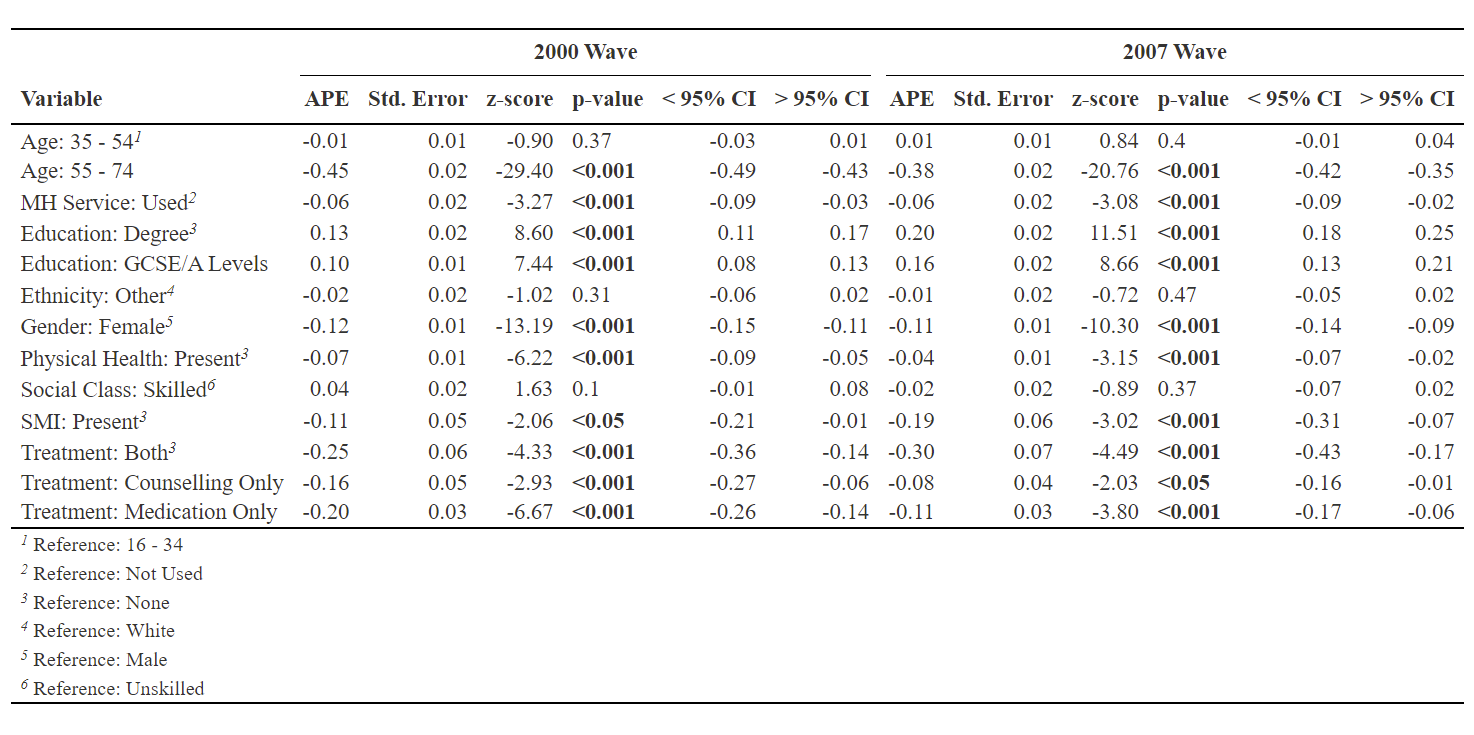
\includegraphics[width=450px,height=300px]{figure/apesmi} \caption[Average Partial Effects for SMI]{Average Partial Effects for SMI in 2000 and 2007}\label{fig:apesmi}
\end{figure}



\begin{figure}
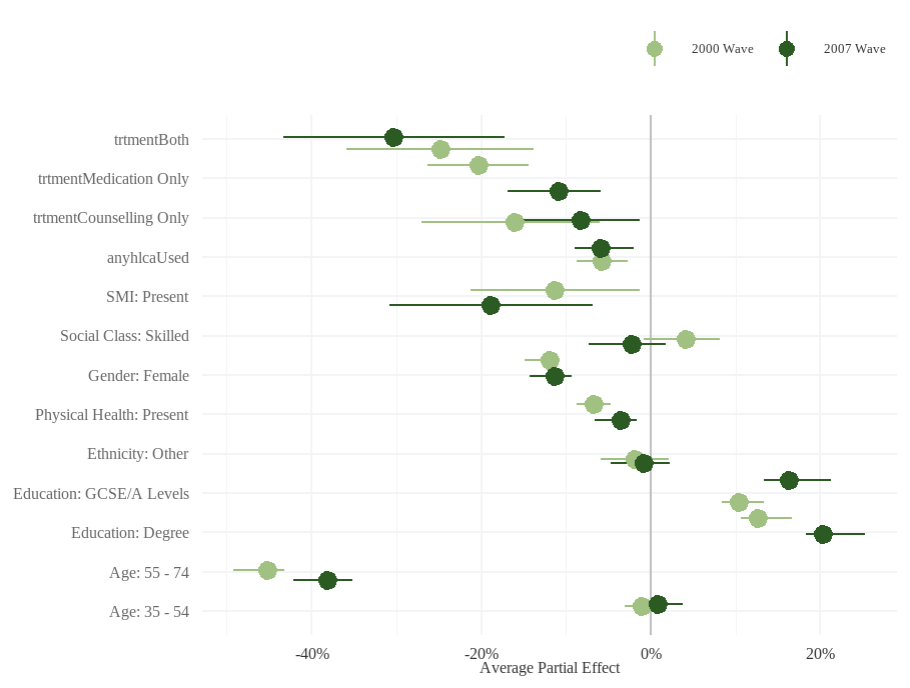
\includegraphics[width=450px,height=300px]{figure/apesmip} \caption[Average Partial Effects Plot for SMI]{Average Partial Effects Plot for SMI in 2000 and 2007}\label{fig:apesmip}
\end{figure}
\hypertarget{goodness-of-fit-for-severe-mental-illness}{%
\subsection{Goodness of Fit for Severe Mental Illness}\label{goodness-of-fit-for-severe-mental-illness}}

Figure \ref{fig:gofsmi} presents the results of the goodness of fit tests on the models for severe mental illness in both survey years. McFadden's R2 values were similar between the two years, with 0.28 for the 2000 survey and 0.24 for the 2007 survey. Despite the similar R2 values, the 2007 survey model did not perform as well as the 2000 survey model. This suggests that the 2007 survey model may not fit the data as well as the 2000 survey model.




\begin{figure}
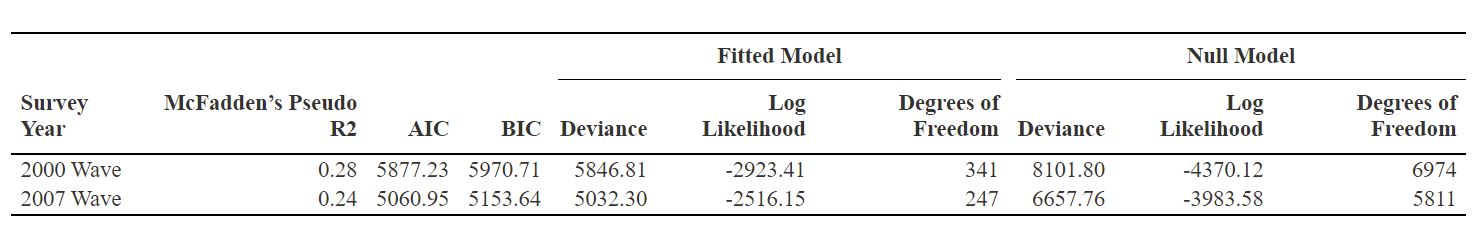
\includegraphics[width=460px,height=100px]{figure/gofsmi} \caption[Goodness of Fit for SMI Models]{Goodness of Fit for SMI Models in 2000 and 2007}\label{fig:gofsmi}
\end{figure}
\hypertarget{severe-mental-illness-type}{%
\section{Severe Mental Illness Type}\label{severe-mental-illness-type}}

In this section the dependent variable was economic activity (being active or not), similar to the previous models. As these are concerned with the impact of severe mental illness on economic activity by type, variables relating to severe mental illness type were added as predictors. These included the conditions of personality disorders, (which included several historical and modern personality disorders, the most prevalent being borderline personality disorder), and psychosis conditions, which can span a wide range of conditions such as schizophrenia, as it is both a symptom of other conditions and a condition in as of itself. As in previous sections in this chapter, logistic regression models were applied to each survey of data, two models in total.

\hypertarget{model-results-for-type-of-severe-mental-illness}{%
\subsection{Model Results for Type of Severe Mental Illness}\label{model-results-for-type-of-severe-mental-illness}}

Adjusted odds ratios and significance levels were similar to the previous models discussed (Table \ref{tab:results2-smitmod}. As in other models, having a degree or GCSE or A Level's was positively associated with being active across both survey waves, and was also statistically significant. Being skilled in the 2000 wave had a small, non-significant association with being active and being aged 35 to 54 years also in the 2007 survey also had a small positive association with being active, but not significant. Being female, aged 55 to 74 years old, being another ethnicity, or having a physical health condition were also negatively associated with being economic active, with gender, age and physical health conditions being statistically significant across both survey waves.

Of the severe mental illness type, both having a psychosis condition or personality disorder were both highly statistically significant and negatively associated with economic activity, with psychosis being more statistically significant than personality disorders in both the 2000 and 2007 survey waves.

\providecommand{\huxb}[2]{\arrayrulecolor[RGB]{#1}\global\arrayrulewidth=#2pt}
  \providecommand{\huxvb}[2]{\color[RGB]{#1}\vrule width #2pt}
  \providecommand{\huxtpad}[1]{\rule{0pt}{#1}}
  \providecommand{\huxbpad}[1]{\rule[-#1]{0pt}{#1}}
\begin{table}[ht]
\begin{centerbox}
\begin{threeparttable}
 \setlength{\tabcolsep}{0pt}
\begin{adjustbox}{width=1\textwidth}
\normalsize
\begin{tabular}{l l l l l l l l l}


\hhline{>{\arrayrulecolor[RGB]{0, 0, 0}\global\arrayrulewidth=0.4pt}->{\arrayrulecolor[RGB]{0, 0, 0}\global\arrayrulewidth=0.4pt}->{\arrayrulecolor[RGB]{0, 0, 0}\global\arrayrulewidth=0.4pt}->{\arrayrulecolor[RGB]{0, 0, 0}\global\arrayrulewidth=0.4pt}->{\arrayrulecolor[RGB]{0, 0, 0}\global\arrayrulewidth=0.4pt}->{\arrayrulecolor[RGB]{0, 0, 0}\global\arrayrulewidth=0.4pt}->{\arrayrulecolor[RGB]{0, 0, 0}\global\arrayrulewidth=0.4pt}->{\arrayrulecolor[RGB]{0, 0, 0}\global\arrayrulewidth=0.4pt}->{\arrayrulecolor[RGB]{0, 0, 0}\global\arrayrulewidth=0.4pt}-}
\arrayrulecolor{black}

\multicolumn{1}{!{\color[RGB]{0, 0, 0}\vrule width 0pt}l!{\color[RGB]{0, 0, 0}\vrule width 0pt}}{\rule{0pt}{1pt + 1em}\raggedright \hspace{0pt} \textbf{{\fontsize{14pt}{16.8pt}\selectfont 
}} \hspace{1pt}\rule[-1pt]{0pt}{1pt}} &
\multicolumn{4}{c!{\color[RGB]{0, 0, 0}\vrule width 0pt}}{\rule{0pt}{1pt + 1em}\centering \hspace{1pt} \textbf{{\fontsize{14pt}{16.8pt}\selectfont \textbf{2000 Wave}
}} \hspace{1pt}\rule[-1pt]{0pt}{1pt}} &
\multicolumn{4}{c!{\color[RGB]{0, 0, 0}\vrule width 0pt}}{\rule{0pt}{1pt + 1em}\centering \hspace{1pt} \textbf{{\fontsize{14pt}{16.8pt}\selectfont \textbf{2007 Wave}
}} \hspace{1pt}\rule[-1pt]{0pt}{1pt}} \tabularnewline[-0.5pt]


\hhline{}
\arrayrulecolor{black}

\multicolumn{1}{!{\color[RGB]{0, 0, 0}\vrule width 0pt}l!{\color[RGB]{0, 0, 0}\vrule width 0pt}}{\rule{0pt}{1pt + 1em}\raggedright \hspace{0pt} \textbf{{\fontsize{14pt}{16.8pt}\selectfont \textbf{Variable}
}} \hspace{1pt}\rule[-1pt]{0pt}{1pt}} &
\multicolumn{1}{c!{\color[RGB]{0, 0, 0}\vrule width 0pt}}{\rule{0pt}{1pt + 1em}\centering \hspace{1pt} \textbf{{\fontsize{14pt}{16.8pt}\selectfont \textbf{N}
}} \hspace{1pt}\rule[-1pt]{0pt}{1pt}} &
\multicolumn{1}{c!{\color[RGB]{0, 0, 0}\vrule width 0pt}}{\rule{0pt}{1pt + 1em}\centering \hspace{1pt} \textbf{{\fontsize{14pt}{16.8pt}\selectfont \textbf{OR}
}} \hspace{1pt}\rule[-1pt]{0pt}{1pt}} &
\multicolumn{1}{c!{\color[RGB]{0, 0, 0}\vrule width 0pt}}{\rule{0pt}{1pt + 1em}\centering \hspace{1pt} \textbf{{\fontsize{14pt}{16.8pt}\selectfont \textbf{95\% CI}
}} \hspace{1pt}\rule[-1pt]{0pt}{1pt}} &
\multicolumn{1}{c!{\color[RGB]{0, 0, 0}\vrule width 0pt}}{\rule{0pt}{1pt + 1em}\centering \hspace{1pt} \textbf{{\fontsize{14pt}{16.8pt}\selectfont \textbf{p-value}
}} \hspace{1pt}\rule[-1pt]{0pt}{1pt}} &
\multicolumn{1}{c!{\color[RGB]{0, 0, 0}\vrule width 0pt}}{\rule{0pt}{1pt + 1em}\centering \hspace{1pt} \textbf{{\fontsize{14pt}{16.8pt}\selectfont \textbf{N}
}} \hspace{1pt}\rule[-1pt]{0pt}{1pt}} &
\multicolumn{1}{c!{\color[RGB]{0, 0, 0}\vrule width 0pt}}{\rule{0pt}{1pt + 1em}\centering \hspace{1pt} \textbf{{\fontsize{14pt}{16.8pt}\selectfont \textbf{OR}
}} \hspace{1pt}\rule[-1pt]{0pt}{1pt}} &
\multicolumn{1}{c!{\color[RGB]{0, 0, 0}\vrule width 0pt}}{\rule{0pt}{1pt + 1em}\centering \hspace{1pt} \textbf{{\fontsize{14pt}{16.8pt}\selectfont \textbf{95\% CI}
}} \hspace{1pt}\rule[-1pt]{0pt}{1pt}} &
\multicolumn{1}{c!{\color[RGB]{0, 0, 0}\vrule width 0pt}}{\rule{0pt}{1pt + 1em}\centering \hspace{1pt} \textbf{{\fontsize{14pt}{16.8pt}\selectfont \textbf{p-value}
}} \hspace{0pt}\rule[-1pt]{0pt}{1pt}} \tabularnewline[-0.5pt]


\hhline{>{\arrayrulecolor[RGB]{0, 0, 0}\global\arrayrulewidth=0.4pt}->{\arrayrulecolor[RGB]{0, 0, 0}\global\arrayrulewidth=0.4pt}->{\arrayrulecolor[RGB]{0, 0, 0}\global\arrayrulewidth=0.4pt}->{\arrayrulecolor[RGB]{0, 0, 0}\global\arrayrulewidth=0.4pt}->{\arrayrulecolor[RGB]{0, 0, 0}\global\arrayrulewidth=0.4pt}->{\arrayrulecolor[RGB]{0, 0, 0}\global\arrayrulewidth=0.4pt}->{\arrayrulecolor[RGB]{0, 0, 0}\global\arrayrulewidth=0.4pt}->{\arrayrulecolor[RGB]{0, 0, 0}\global\arrayrulewidth=0.4pt}->{\arrayrulecolor[RGB]{0, 0, 0}\global\arrayrulewidth=0.4pt}-}
\arrayrulecolor{black}

\multicolumn{1}{!{\color[RGB]{0, 0, 0}\vrule width 0pt}l!{\color[RGB]{0, 0, 0}\vrule width 0pt}}{\rule{0pt}{1pt + 1em}\raggedright \hspace{0pt} \textbf{{\fontsize{14pt}{16.8pt}\selectfont SMI Type}} \hspace{1pt}\rule[-1pt]{0pt}{1pt}} &
\multicolumn{1}{c!{\color[RGB]{0, 0, 0}\vrule width 0pt}}{\rule{0pt}{1pt + 1em}\centering \hspace{1pt} {\fontsize{14pt}{16.8pt}\selectfont 6,920} \hspace{1pt}\rule[-1pt]{0pt}{1pt}} &
\multicolumn{1}{c!{\color[RGB]{0, 0, 0}\vrule width 0pt}}{\rule{0pt}{1pt + 1em}\centering \hspace{1pt} {\fontsize{14pt}{16.8pt}\selectfont } \hspace{1pt}\rule[-1pt]{0pt}{1pt}} &
\multicolumn{1}{c!{\color[RGB]{0, 0, 0}\vrule width 0pt}}{\rule{0pt}{1pt + 1em}\centering \hspace{1pt} {\fontsize{14pt}{16.8pt}\selectfont } \hspace{1pt}\rule[-1pt]{0pt}{1pt}} &
\multicolumn{1}{c!{\color[RGB]{0, 0, 0}\vrule width 0pt}}{\rule{0pt}{1pt + 1em}\centering \hspace{1pt} {\fontsize{14pt}{16.8pt}\selectfont } \hspace{1pt}\rule[-1pt]{0pt}{1pt}} &
\multicolumn{1}{c!{\color[RGB]{0, 0, 0}\vrule width 0pt}}{\rule{0pt}{1pt + 1em}\centering \hspace{1pt} {\fontsize{14pt}{16.8pt}\selectfont 5,750} \hspace{1pt}\rule[-1pt]{0pt}{1pt}} &
\multicolumn{1}{c!{\color[RGB]{0, 0, 0}\vrule width 0pt}}{\rule{0pt}{1pt + 1em}\centering \hspace{1pt} {\fontsize{14pt}{16.8pt}\selectfont } \hspace{1pt}\rule[-1pt]{0pt}{1pt}} &
\multicolumn{1}{c!{\color[RGB]{0, 0, 0}\vrule width 0pt}}{\rule{0pt}{1pt + 1em}\centering \hspace{1pt} {\fontsize{14pt}{16.8pt}\selectfont } \hspace{1pt}\rule[-1pt]{0pt}{1pt}} &
\multicolumn{1}{c!{\color[RGB]{0, 0, 0}\vrule width 0pt}}{\rule{0pt}{1pt + 1em}\centering \hspace{1pt} {\fontsize{14pt}{16.8pt}\selectfont } \hspace{0pt}\rule[-1pt]{0pt}{1pt}} \tabularnewline[-0.5pt]


\hhline{}
\arrayrulecolor{black}

\multicolumn{1}{!{\color[RGB]{0, 0, 0}\vrule width 0pt}l!{\color[RGB]{0, 0, 0}\vrule width 0pt}}{\rule{0pt}{1pt + 1em}\raggedright \hspace{0pt} {\fontsize{14pt}{16.8pt}\selectfont None} \hspace{1pt}\rule[-1pt]{0pt}{1pt}} &
\multicolumn{1}{c!{\color[RGB]{0, 0, 0}\vrule width 0pt}}{\rule{0pt}{1pt + 1em}\centering \hspace{1pt} {\fontsize{14pt}{16.8pt}\selectfont } \hspace{1pt}\rule[-1pt]{0pt}{1pt}} &
\multicolumn{1}{c!{\color[RGB]{0, 0, 0}\vrule width 0pt}}{\rule{0pt}{1pt + 1em}\centering \hspace{1pt} {\fontsize{14pt}{16.8pt}\selectfont —} \hspace{1pt}\rule[-1pt]{0pt}{1pt}} &
\multicolumn{1}{c!{\color[RGB]{0, 0, 0}\vrule width 0pt}}{\rule{0pt}{1pt + 1em}\centering \hspace{1pt} {\fontsize{14pt}{16.8pt}\selectfont —} \hspace{1pt}\rule[-1pt]{0pt}{1pt}} &
\multicolumn{1}{c!{\color[RGB]{0, 0, 0}\vrule width 0pt}}{\rule{0pt}{1pt + 1em}\centering \hspace{1pt} {\fontsize{14pt}{16.8pt}\selectfont } \hspace{1pt}\rule[-1pt]{0pt}{1pt}} &
\multicolumn{1}{c!{\color[RGB]{0, 0, 0}\vrule width 0pt}}{\rule{0pt}{1pt + 1em}\centering \hspace{1pt} {\fontsize{14pt}{16.8pt}\selectfont } \hspace{1pt}\rule[-1pt]{0pt}{1pt}} &
\multicolumn{1}{c!{\color[RGB]{0, 0, 0}\vrule width 0pt}}{\rule{0pt}{1pt + 1em}\centering \hspace{1pt} {\fontsize{14pt}{16.8pt}\selectfont —} \hspace{1pt}\rule[-1pt]{0pt}{1pt}} &
\multicolumn{1}{c!{\color[RGB]{0, 0, 0}\vrule width 0pt}}{\rule{0pt}{1pt + 1em}\centering \hspace{1pt} {\fontsize{14pt}{16.8pt}\selectfont —} \hspace{1pt}\rule[-1pt]{0pt}{1pt}} &
\multicolumn{1}{c!{\color[RGB]{0, 0, 0}\vrule width 0pt}}{\rule{0pt}{1pt + 1em}\centering \hspace{1pt} {\fontsize{14pt}{16.8pt}\selectfont } \hspace{0pt}\rule[-1pt]{0pt}{1pt}} \tabularnewline[-0.5pt]


\hhline{}
\arrayrulecolor{black}

\multicolumn{1}{!{\color[RGB]{0, 0, 0}\vrule width 0pt}l!{\color[RGB]{0, 0, 0}\vrule width 0pt}}{\rule{0pt}{1pt + 1em}\raggedright \hspace{0pt} {\fontsize{14pt}{16.8pt}\selectfont Personality Disorder} \hspace{1pt}\rule[-1pt]{0pt}{1pt}} &
\multicolumn{1}{c!{\color[RGB]{0, 0, 0}\vrule width 0pt}}{\rule{0pt}{1pt + 1em}\centering \hspace{1pt} {\fontsize{14pt}{16.8pt}\selectfont } \hspace{1pt}\rule[-1pt]{0pt}{1pt}} &
\multicolumn{1}{c!{\color[RGB]{0, 0, 0}\vrule width 0pt}}{\rule{0pt}{1pt + 1em}\centering \hspace{1pt} {\fontsize{14pt}{16.8pt}\selectfont 0.31} \hspace{1pt}\rule[-1pt]{0pt}{1pt}} &
\multicolumn{1}{c!{\color[RGB]{0, 0, 0}\vrule width 0pt}}{\rule{0pt}{1pt + 1em}\centering \hspace{1pt} {\fontsize{14pt}{16.8pt}\selectfont 0.14, 0.66} \hspace{1pt}\rule[-1pt]{0pt}{1pt}} &
\multicolumn{1}{c!{\color[RGB]{0, 0, 0}\vrule width 0pt}}{\rule{0pt}{1pt + 1em}\centering \hspace{1pt} \textbf{{\fontsize{14pt}{16.8pt}\selectfont 0.002}} \hspace{1pt}\rule[-1pt]{0pt}{1pt}} &
\multicolumn{1}{c!{\color[RGB]{0, 0, 0}\vrule width 0pt}}{\rule{0pt}{1pt + 1em}\centering \hspace{1pt} {\fontsize{14pt}{16.8pt}\selectfont } \hspace{1pt}\rule[-1pt]{0pt}{1pt}} &
\multicolumn{1}{c!{\color[RGB]{0, 0, 0}\vrule width 0pt}}{\rule{0pt}{1pt + 1em}\centering \hspace{1pt} {\fontsize{14pt}{16.8pt}\selectfont 0.23} \hspace{1pt}\rule[-1pt]{0pt}{1pt}} &
\multicolumn{1}{c!{\color[RGB]{0, 0, 0}\vrule width 0pt}}{\rule{0pt}{1pt + 1em}\centering \hspace{1pt} {\fontsize{14pt}{16.8pt}\selectfont 0.09, 0.63} \hspace{1pt}\rule[-1pt]{0pt}{1pt}} &
\multicolumn{1}{c!{\color[RGB]{0, 0, 0}\vrule width 0pt}}{\rule{0pt}{1pt + 1em}\centering \hspace{1pt} \textbf{{\fontsize{14pt}{16.8pt}\selectfont 0.004}} \hspace{0pt}\rule[-1pt]{0pt}{1pt}} \tabularnewline[-0.5pt]


\hhline{}
\arrayrulecolor{black}

\multicolumn{1}{!{\color[RGB]{0, 0, 0}\vrule width 0pt}l!{\color[RGB]{0, 0, 0}\vrule width 0pt}}{\rule{0pt}{1pt + 1em}\raggedright \hspace{0pt} {\fontsize{14pt}{16.8pt}\selectfont Psychosis Condition} \hspace{1pt}\rule[-1pt]{0pt}{1pt}} &
\multicolumn{1}{c!{\color[RGB]{0, 0, 0}\vrule width 0pt}}{\rule{0pt}{1pt + 1em}\centering \hspace{1pt} {\fontsize{14pt}{16.8pt}\selectfont } \hspace{1pt}\rule[-1pt]{0pt}{1pt}} &
\multicolumn{1}{c!{\color[RGB]{0, 0, 0}\vrule width 0pt}}{\rule{0pt}{1pt + 1em}\centering \hspace{1pt} {\fontsize{14pt}{16.8pt}\selectfont 0.10} \hspace{1pt}\rule[-1pt]{0pt}{1pt}} &
\multicolumn{1}{c!{\color[RGB]{0, 0, 0}\vrule width 0pt}}{\rule{0pt}{1pt + 1em}\centering \hspace{1pt} {\fontsize{14pt}{16.8pt}\selectfont 0.04, 0.21} \hspace{1pt}\rule[-1pt]{0pt}{1pt}} &
\multicolumn{1}{c!{\color[RGB]{0, 0, 0}\vrule width 0pt}}{\rule{0pt}{1pt + 1em}\centering \hspace{1pt} \textbf{{\fontsize{14pt}{16.8pt}\selectfont $<$0.001}} \hspace{1pt}\rule[-1pt]{0pt}{1pt}} &
\multicolumn{1}{c!{\color[RGB]{0, 0, 0}\vrule width 0pt}}{\rule{0pt}{1pt + 1em}\centering \hspace{1pt} {\fontsize{14pt}{16.8pt}\selectfont } \hspace{1pt}\rule[-1pt]{0pt}{1pt}} &
\multicolumn{1}{c!{\color[RGB]{0, 0, 0}\vrule width 0pt}}{\rule{0pt}{1pt + 1em}\centering \hspace{1pt} {\fontsize{14pt}{16.8pt}\selectfont 0.12} \hspace{1pt}\rule[-1pt]{0pt}{1pt}} &
\multicolumn{1}{c!{\color[RGB]{0, 0, 0}\vrule width 0pt}}{\rule{0pt}{1pt + 1em}\centering \hspace{1pt} {\fontsize{14pt}{16.8pt}\selectfont 0.04, 0.31} \hspace{1pt}\rule[-1pt]{0pt}{1pt}} &
\multicolumn{1}{c!{\color[RGB]{0, 0, 0}\vrule width 0pt}}{\rule{0pt}{1pt + 1em}\centering \hspace{1pt} \textbf{{\fontsize{14pt}{16.8pt}\selectfont $<$0.001}} \hspace{0pt}\rule[-1pt]{0pt}{1pt}} \tabularnewline[-0.5pt]


\hhline{}
\arrayrulecolor{black}

\multicolumn{1}{!{\color[RGB]{0, 0, 0}\vrule width 0pt}l!{\color[RGB]{0, 0, 0}\vrule width 0pt}}{\rule{0pt}{1pt + 1em}\raggedright \hspace{0pt} \textbf{{\fontsize{14pt}{16.8pt}\selectfont Gender}} \hspace{1pt}\rule[-1pt]{0pt}{1pt}} &
\multicolumn{1}{c!{\color[RGB]{0, 0, 0}\vrule width 0pt}}{\rule{0pt}{1pt + 1em}\centering \hspace{1pt} {\fontsize{14pt}{16.8pt}\selectfont 6,920} \hspace{1pt}\rule[-1pt]{0pt}{1pt}} &
\multicolumn{1}{c!{\color[RGB]{0, 0, 0}\vrule width 0pt}}{\rule{0pt}{1pt + 1em}\centering \hspace{1pt} {\fontsize{14pt}{16.8pt}\selectfont } \hspace{1pt}\rule[-1pt]{0pt}{1pt}} &
\multicolumn{1}{c!{\color[RGB]{0, 0, 0}\vrule width 0pt}}{\rule{0pt}{1pt + 1em}\centering \hspace{1pt} {\fontsize{14pt}{16.8pt}\selectfont } \hspace{1pt}\rule[-1pt]{0pt}{1pt}} &
\multicolumn{1}{c!{\color[RGB]{0, 0, 0}\vrule width 0pt}}{\rule{0pt}{1pt + 1em}\centering \hspace{1pt} {\fontsize{14pt}{16.8pt}\selectfont } \hspace{1pt}\rule[-1pt]{0pt}{1pt}} &
\multicolumn{1}{c!{\color[RGB]{0, 0, 0}\vrule width 0pt}}{\rule{0pt}{1pt + 1em}\centering \hspace{1pt} {\fontsize{14pt}{16.8pt}\selectfont 5,750} \hspace{1pt}\rule[-1pt]{0pt}{1pt}} &
\multicolumn{1}{c!{\color[RGB]{0, 0, 0}\vrule width 0pt}}{\rule{0pt}{1pt + 1em}\centering \hspace{1pt} {\fontsize{14pt}{16.8pt}\selectfont } \hspace{1pt}\rule[-1pt]{0pt}{1pt}} &
\multicolumn{1}{c!{\color[RGB]{0, 0, 0}\vrule width 0pt}}{\rule{0pt}{1pt + 1em}\centering \hspace{1pt} {\fontsize{14pt}{16.8pt}\selectfont } \hspace{1pt}\rule[-1pt]{0pt}{1pt}} &
\multicolumn{1}{c!{\color[RGB]{0, 0, 0}\vrule width 0pt}}{\rule{0pt}{1pt + 1em}\centering \hspace{1pt} {\fontsize{14pt}{16.8pt}\selectfont } \hspace{0pt}\rule[-1pt]{0pt}{1pt}} \tabularnewline[-0.5pt]


\hhline{}
\arrayrulecolor{black}

\multicolumn{1}{!{\color[RGB]{0, 0, 0}\vrule width 0pt}l!{\color[RGB]{0, 0, 0}\vrule width 0pt}}{\rule{0pt}{1pt + 1em}\raggedright \hspace{0pt} {\fontsize{14pt}{16.8pt}\selectfont Male} \hspace{1pt}\rule[-1pt]{0pt}{1pt}} &
\multicolumn{1}{c!{\color[RGB]{0, 0, 0}\vrule width 0pt}}{\rule{0pt}{1pt + 1em}\centering \hspace{1pt} {\fontsize{14pt}{16.8pt}\selectfont } \hspace{1pt}\rule[-1pt]{0pt}{1pt}} &
\multicolumn{1}{c!{\color[RGB]{0, 0, 0}\vrule width 0pt}}{\rule{0pt}{1pt + 1em}\centering \hspace{1pt} {\fontsize{14pt}{16.8pt}\selectfont —} \hspace{1pt}\rule[-1pt]{0pt}{1pt}} &
\multicolumn{1}{c!{\color[RGB]{0, 0, 0}\vrule width 0pt}}{\rule{0pt}{1pt + 1em}\centering \hspace{1pt} {\fontsize{14pt}{16.8pt}\selectfont —} \hspace{1pt}\rule[-1pt]{0pt}{1pt}} &
\multicolumn{1}{c!{\color[RGB]{0, 0, 0}\vrule width 0pt}}{\rule{0pt}{1pt + 1em}\centering \hspace{1pt} {\fontsize{14pt}{16.8pt}\selectfont } \hspace{1pt}\rule[-1pt]{0pt}{1pt}} &
\multicolumn{1}{c!{\color[RGB]{0, 0, 0}\vrule width 0pt}}{\rule{0pt}{1pt + 1em}\centering \hspace{1pt} {\fontsize{14pt}{16.8pt}\selectfont } \hspace{1pt}\rule[-1pt]{0pt}{1pt}} &
\multicolumn{1}{c!{\color[RGB]{0, 0, 0}\vrule width 0pt}}{\rule{0pt}{1pt + 1em}\centering \hspace{1pt} {\fontsize{14pt}{16.8pt}\selectfont —} \hspace{1pt}\rule[-1pt]{0pt}{1pt}} &
\multicolumn{1}{c!{\color[RGB]{0, 0, 0}\vrule width 0pt}}{\rule{0pt}{1pt + 1em}\centering \hspace{1pt} {\fontsize{14pt}{16.8pt}\selectfont —} \hspace{1pt}\rule[-1pt]{0pt}{1pt}} &
\multicolumn{1}{c!{\color[RGB]{0, 0, 0}\vrule width 0pt}}{\rule{0pt}{1pt + 1em}\centering \hspace{1pt} {\fontsize{14pt}{16.8pt}\selectfont } \hspace{0pt}\rule[-1pt]{0pt}{1pt}} \tabularnewline[-0.5pt]


\hhline{}
\arrayrulecolor{black}

\multicolumn{1}{!{\color[RGB]{0, 0, 0}\vrule width 0pt}l!{\color[RGB]{0, 0, 0}\vrule width 0pt}}{\rule{0pt}{1pt + 1em}\raggedright \hspace{0pt} {\fontsize{14pt}{16.8pt}\selectfont Female} \hspace{1pt}\rule[-1pt]{0pt}{1pt}} &
\multicolumn{1}{c!{\color[RGB]{0, 0, 0}\vrule width 0pt}}{\rule{0pt}{1pt + 1em}\centering \hspace{1pt} {\fontsize{14pt}{16.8pt}\selectfont } \hspace{1pt}\rule[-1pt]{0pt}{1pt}} &
\multicolumn{1}{c!{\color[RGB]{0, 0, 0}\vrule width 0pt}}{\rule{0pt}{1pt + 1em}\centering \hspace{1pt} {\fontsize{14pt}{16.8pt}\selectfont 0.38} \hspace{1pt}\rule[-1pt]{0pt}{1pt}} &
\multicolumn{1}{c!{\color[RGB]{0, 0, 0}\vrule width 0pt}}{\rule{0pt}{1pt + 1em}\centering \hspace{1pt} {\fontsize{14pt}{16.8pt}\selectfont 0.33, 0.43} \hspace{1pt}\rule[-1pt]{0pt}{1pt}} &
\multicolumn{1}{c!{\color[RGB]{0, 0, 0}\vrule width 0pt}}{\rule{0pt}{1pt + 1em}\centering \hspace{1pt} \textbf{{\fontsize{14pt}{16.8pt}\selectfont $<$0.001}} \hspace{1pt}\rule[-1pt]{0pt}{1pt}} &
\multicolumn{1}{c!{\color[RGB]{0, 0, 0}\vrule width 0pt}}{\rule{0pt}{1pt + 1em}\centering \hspace{1pt} {\fontsize{14pt}{16.8pt}\selectfont } \hspace{1pt}\rule[-1pt]{0pt}{1pt}} &
\multicolumn{1}{c!{\color[RGB]{0, 0, 0}\vrule width 0pt}}{\rule{0pt}{1pt + 1em}\centering \hspace{1pt} {\fontsize{14pt}{16.8pt}\selectfont 0.44} \hspace{1pt}\rule[-1pt]{0pt}{1pt}} &
\multicolumn{1}{c!{\color[RGB]{0, 0, 0}\vrule width 0pt}}{\rule{0pt}{1pt + 1em}\centering \hspace{1pt} {\fontsize{14pt}{16.8pt}\selectfont 0.38, 0.51} \hspace{1pt}\rule[-1pt]{0pt}{1pt}} &
\multicolumn{1}{c!{\color[RGB]{0, 0, 0}\vrule width 0pt}}{\rule{0pt}{1pt + 1em}\centering \hspace{1pt} \textbf{{\fontsize{14pt}{16.8pt}\selectfont $<$0.001}} \hspace{0pt}\rule[-1pt]{0pt}{1pt}} \tabularnewline[-0.5pt]


\hhline{}
\arrayrulecolor{black}

\multicolumn{1}{!{\color[RGB]{0, 0, 0}\vrule width 0pt}l!{\color[RGB]{0, 0, 0}\vrule width 0pt}}{\rule{0pt}{1pt + 1em}\raggedright \hspace{0pt} \textbf{{\fontsize{14pt}{16.8pt}\selectfont Age Band}} \hspace{1pt}\rule[-1pt]{0pt}{1pt}} &
\multicolumn{1}{c!{\color[RGB]{0, 0, 0}\vrule width 0pt}}{\rule{0pt}{1pt + 1em}\centering \hspace{1pt} {\fontsize{14pt}{16.8pt}\selectfont 6,920} \hspace{1pt}\rule[-1pt]{0pt}{1pt}} &
\multicolumn{1}{c!{\color[RGB]{0, 0, 0}\vrule width 0pt}}{\rule{0pt}{1pt + 1em}\centering \hspace{1pt} {\fontsize{14pt}{16.8pt}\selectfont } \hspace{1pt}\rule[-1pt]{0pt}{1pt}} &
\multicolumn{1}{c!{\color[RGB]{0, 0, 0}\vrule width 0pt}}{\rule{0pt}{1pt + 1em}\centering \hspace{1pt} {\fontsize{14pt}{16.8pt}\selectfont } \hspace{1pt}\rule[-1pt]{0pt}{1pt}} &
\multicolumn{1}{c!{\color[RGB]{0, 0, 0}\vrule width 0pt}}{\rule{0pt}{1pt + 1em}\centering \hspace{1pt} {\fontsize{14pt}{16.8pt}\selectfont } \hspace{1pt}\rule[-1pt]{0pt}{1pt}} &
\multicolumn{1}{c!{\color[RGB]{0, 0, 0}\vrule width 0pt}}{\rule{0pt}{1pt + 1em}\centering \hspace{1pt} {\fontsize{14pt}{16.8pt}\selectfont 5,750} \hspace{1pt}\rule[-1pt]{0pt}{1pt}} &
\multicolumn{1}{c!{\color[RGB]{0, 0, 0}\vrule width 0pt}}{\rule{0pt}{1pt + 1em}\centering \hspace{1pt} {\fontsize{14pt}{16.8pt}\selectfont } \hspace{1pt}\rule[-1pt]{0pt}{1pt}} &
\multicolumn{1}{c!{\color[RGB]{0, 0, 0}\vrule width 0pt}}{\rule{0pt}{1pt + 1em}\centering \hspace{1pt} {\fontsize{14pt}{16.8pt}\selectfont } \hspace{1pt}\rule[-1pt]{0pt}{1pt}} &
\multicolumn{1}{c!{\color[RGB]{0, 0, 0}\vrule width 0pt}}{\rule{0pt}{1pt + 1em}\centering \hspace{1pt} {\fontsize{14pt}{16.8pt}\selectfont } \hspace{0pt}\rule[-1pt]{0pt}{1pt}} \tabularnewline[-0.5pt]


\hhline{}
\arrayrulecolor{black}

\multicolumn{1}{!{\color[RGB]{0, 0, 0}\vrule width 0pt}l!{\color[RGB]{0, 0, 0}\vrule width 0pt}}{\rule{0pt}{1pt + 1em}\raggedright \hspace{0pt} {\fontsize{14pt}{16.8pt}\selectfont 16 - 34} \hspace{1pt}\rule[-1pt]{0pt}{1pt}} &
\multicolumn{1}{c!{\color[RGB]{0, 0, 0}\vrule width 0pt}}{\rule{0pt}{1pt + 1em}\centering \hspace{1pt} {\fontsize{14pt}{16.8pt}\selectfont } \hspace{1pt}\rule[-1pt]{0pt}{1pt}} &
\multicolumn{1}{c!{\color[RGB]{0, 0, 0}\vrule width 0pt}}{\rule{0pt}{1pt + 1em}\centering \hspace{1pt} {\fontsize{14pt}{16.8pt}\selectfont —} \hspace{1pt}\rule[-1pt]{0pt}{1pt}} &
\multicolumn{1}{c!{\color[RGB]{0, 0, 0}\vrule width 0pt}}{\rule{0pt}{1pt + 1em}\centering \hspace{1pt} {\fontsize{14pt}{16.8pt}\selectfont —} \hspace{1pt}\rule[-1pt]{0pt}{1pt}} &
\multicolumn{1}{c!{\color[RGB]{0, 0, 0}\vrule width 0pt}}{\rule{0pt}{1pt + 1em}\centering \hspace{1pt} {\fontsize{14pt}{16.8pt}\selectfont } \hspace{1pt}\rule[-1pt]{0pt}{1pt}} &
\multicolumn{1}{c!{\color[RGB]{0, 0, 0}\vrule width 0pt}}{\rule{0pt}{1pt + 1em}\centering \hspace{1pt} {\fontsize{14pt}{16.8pt}\selectfont } \hspace{1pt}\rule[-1pt]{0pt}{1pt}} &
\multicolumn{1}{c!{\color[RGB]{0, 0, 0}\vrule width 0pt}}{\rule{0pt}{1pt + 1em}\centering \hspace{1pt} {\fontsize{14pt}{16.8pt}\selectfont —} \hspace{1pt}\rule[-1pt]{0pt}{1pt}} &
\multicolumn{1}{c!{\color[RGB]{0, 0, 0}\vrule width 0pt}}{\rule{0pt}{1pt + 1em}\centering \hspace{1pt} {\fontsize{14pt}{16.8pt}\selectfont —} \hspace{1pt}\rule[-1pt]{0pt}{1pt}} &
\multicolumn{1}{c!{\color[RGB]{0, 0, 0}\vrule width 0pt}}{\rule{0pt}{1pt + 1em}\centering \hspace{1pt} {\fontsize{14pt}{16.8pt}\selectfont } \hspace{0pt}\rule[-1pt]{0pt}{1pt}} \tabularnewline[-0.5pt]


\hhline{}
\arrayrulecolor{black}

\multicolumn{1}{!{\color[RGB]{0, 0, 0}\vrule width 0pt}l!{\color[RGB]{0, 0, 0}\vrule width 0pt}}{\rule{0pt}{1pt + 1em}\raggedright \hspace{0pt} {\fontsize{14pt}{16.8pt}\selectfont 35 - 54} \hspace{1pt}\rule[-1pt]{0pt}{1pt}} &
\multicolumn{1}{c!{\color[RGB]{0, 0, 0}\vrule width 0pt}}{\rule{0pt}{1pt + 1em}\centering \hspace{1pt} {\fontsize{14pt}{16.8pt}\selectfont } \hspace{1pt}\rule[-1pt]{0pt}{1pt}} &
\multicolumn{1}{c!{\color[RGB]{0, 0, 0}\vrule width 0pt}}{\rule{0pt}{1pt + 1em}\centering \hspace{1pt} {\fontsize{14pt}{16.8pt}\selectfont 0.87} \hspace{1pt}\rule[-1pt]{0pt}{1pt}} &
\multicolumn{1}{c!{\color[RGB]{0, 0, 0}\vrule width 0pt}}{\rule{0pt}{1pt + 1em}\centering \hspace{1pt} {\fontsize{14pt}{16.8pt}\selectfont 0.74, 1.03} \hspace{1pt}\rule[-1pt]{0pt}{1pt}} &
\multicolumn{1}{c!{\color[RGB]{0, 0, 0}\vrule width 0pt}}{\rule{0pt}{1pt + 1em}\centering \hspace{1pt} {\fontsize{14pt}{16.8pt}\selectfont 0.10} \hspace{1pt}\rule[-1pt]{0pt}{1pt}} &
\multicolumn{1}{c!{\color[RGB]{0, 0, 0}\vrule width 0pt}}{\rule{0pt}{1pt + 1em}\centering \hspace{1pt} {\fontsize{14pt}{16.8pt}\selectfont } \hspace{1pt}\rule[-1pt]{0pt}{1pt}} &
\multicolumn{1}{c!{\color[RGB]{0, 0, 0}\vrule width 0pt}}{\rule{0pt}{1pt + 1em}\centering \hspace{1pt} {\fontsize{14pt}{16.8pt}\selectfont 1.05} \hspace{1pt}\rule[-1pt]{0pt}{1pt}} &
\multicolumn{1}{c!{\color[RGB]{0, 0, 0}\vrule width 0pt}}{\rule{0pt}{1pt + 1em}\centering \hspace{1pt} {\fontsize{14pt}{16.8pt}\selectfont 0.84, 1.32} \hspace{1pt}\rule[-1pt]{0pt}{1pt}} &
\multicolumn{1}{c!{\color[RGB]{0, 0, 0}\vrule width 0pt}}{\rule{0pt}{1pt + 1em}\centering \hspace{1pt} {\fontsize{14pt}{16.8pt}\selectfont 0.66} \hspace{0pt}\rule[-1pt]{0pt}{1pt}} \tabularnewline[-0.5pt]


\hhline{}
\arrayrulecolor{black}

\multicolumn{1}{!{\color[RGB]{0, 0, 0}\vrule width 0pt}l!{\color[RGB]{0, 0, 0}\vrule width 0pt}}{\rule{0pt}{1pt + 1em}\raggedright \hspace{0pt} {\fontsize{14pt}{16.8pt}\selectfont 55 - 74} \hspace{1pt}\rule[-1pt]{0pt}{1pt}} &
\multicolumn{1}{c!{\color[RGB]{0, 0, 0}\vrule width 0pt}}{\rule{0pt}{1pt + 1em}\centering \hspace{1pt} {\fontsize{14pt}{16.8pt}\selectfont } \hspace{1pt}\rule[-1pt]{0pt}{1pt}} &
\multicolumn{1}{c!{\color[RGB]{0, 0, 0}\vrule width 0pt}}{\rule{0pt}{1pt + 1em}\centering \hspace{1pt} {\fontsize{14pt}{16.8pt}\selectfont 0.09} \hspace{1pt}\rule[-1pt]{0pt}{1pt}} &
\multicolumn{1}{c!{\color[RGB]{0, 0, 0}\vrule width 0pt}}{\rule{0pt}{1pt + 1em}\centering \hspace{1pt} {\fontsize{14pt}{16.8pt}\selectfont 0.08, 0.11} \hspace{1pt}\rule[-1pt]{0pt}{1pt}} &
\multicolumn{1}{c!{\color[RGB]{0, 0, 0}\vrule width 0pt}}{\rule{0pt}{1pt + 1em}\centering \hspace{1pt} \textbf{{\fontsize{14pt}{16.8pt}\selectfont $<$0.001}} \hspace{1pt}\rule[-1pt]{0pt}{1pt}} &
\multicolumn{1}{c!{\color[RGB]{0, 0, 0}\vrule width 0pt}}{\rule{0pt}{1pt + 1em}\centering \hspace{1pt} {\fontsize{14pt}{16.8pt}\selectfont } \hspace{1pt}\rule[-1pt]{0pt}{1pt}} &
\multicolumn{1}{c!{\color[RGB]{0, 0, 0}\vrule width 0pt}}{\rule{0pt}{1pt + 1em}\centering \hspace{1pt} {\fontsize{14pt}{16.8pt}\selectfont 0.14} \hspace{1pt}\rule[-1pt]{0pt}{1pt}} &
\multicolumn{1}{c!{\color[RGB]{0, 0, 0}\vrule width 0pt}}{\rule{0pt}{1pt + 1em}\centering \hspace{1pt} {\fontsize{14pt}{16.8pt}\selectfont 0.11, 0.17} \hspace{1pt}\rule[-1pt]{0pt}{1pt}} &
\multicolumn{1}{c!{\color[RGB]{0, 0, 0}\vrule width 0pt}}{\rule{0pt}{1pt + 1em}\centering \hspace{1pt} \textbf{{\fontsize{14pt}{16.8pt}\selectfont $<$0.001}} \hspace{0pt}\rule[-1pt]{0pt}{1pt}} \tabularnewline[-0.5pt]


\hhline{}
\arrayrulecolor{black}

\multicolumn{1}{!{\color[RGB]{0, 0, 0}\vrule width 0pt}l!{\color[RGB]{0, 0, 0}\vrule width 0pt}}{\rule{0pt}{1pt + 1em}\raggedright \hspace{0pt} \textbf{{\fontsize{14pt}{16.8pt}\selectfont Ethnicity}} \hspace{1pt}\rule[-1pt]{0pt}{1pt}} &
\multicolumn{1}{c!{\color[RGB]{0, 0, 0}\vrule width 0pt}}{\rule{0pt}{1pt + 1em}\centering \hspace{1pt} {\fontsize{14pt}{16.8pt}\selectfont 6,920} \hspace{1pt}\rule[-1pt]{0pt}{1pt}} &
\multicolumn{1}{c!{\color[RGB]{0, 0, 0}\vrule width 0pt}}{\rule{0pt}{1pt + 1em}\centering \hspace{1pt} {\fontsize{14pt}{16.8pt}\selectfont } \hspace{1pt}\rule[-1pt]{0pt}{1pt}} &
\multicolumn{1}{c!{\color[RGB]{0, 0, 0}\vrule width 0pt}}{\rule{0pt}{1pt + 1em}\centering \hspace{1pt} {\fontsize{14pt}{16.8pt}\selectfont } \hspace{1pt}\rule[-1pt]{0pt}{1pt}} &
\multicolumn{1}{c!{\color[RGB]{0, 0, 0}\vrule width 0pt}}{\rule{0pt}{1pt + 1em}\centering \hspace{1pt} {\fontsize{14pt}{16.8pt}\selectfont } \hspace{1pt}\rule[-1pt]{0pt}{1pt}} &
\multicolumn{1}{c!{\color[RGB]{0, 0, 0}\vrule width 0pt}}{\rule{0pt}{1pt + 1em}\centering \hspace{1pt} {\fontsize{14pt}{16.8pt}\selectfont 5,750} \hspace{1pt}\rule[-1pt]{0pt}{1pt}} &
\multicolumn{1}{c!{\color[RGB]{0, 0, 0}\vrule width 0pt}}{\rule{0pt}{1pt + 1em}\centering \hspace{1pt} {\fontsize{14pt}{16.8pt}\selectfont } \hspace{1pt}\rule[-1pt]{0pt}{1pt}} &
\multicolumn{1}{c!{\color[RGB]{0, 0, 0}\vrule width 0pt}}{\rule{0pt}{1pt + 1em}\centering \hspace{1pt} {\fontsize{14pt}{16.8pt}\selectfont } \hspace{1pt}\rule[-1pt]{0pt}{1pt}} &
\multicolumn{1}{c!{\color[RGB]{0, 0, 0}\vrule width 0pt}}{\rule{0pt}{1pt + 1em}\centering \hspace{1pt} {\fontsize{14pt}{16.8pt}\selectfont } \hspace{0pt}\rule[-1pt]{0pt}{1pt}} \tabularnewline[-0.5pt]


\hhline{}
\arrayrulecolor{black}

\multicolumn{1}{!{\color[RGB]{0, 0, 0}\vrule width 0pt}l!{\color[RGB]{0, 0, 0}\vrule width 0pt}}{\rule{0pt}{1pt + 1em}\raggedright \hspace{0pt} {\fontsize{14pt}{16.8pt}\selectfont White} \hspace{1pt}\rule[-1pt]{0pt}{1pt}} &
\multicolumn{1}{c!{\color[RGB]{0, 0, 0}\vrule width 0pt}}{\rule{0pt}{1pt + 1em}\centering \hspace{1pt} {\fontsize{14pt}{16.8pt}\selectfont } \hspace{1pt}\rule[-1pt]{0pt}{1pt}} &
\multicolumn{1}{c!{\color[RGB]{0, 0, 0}\vrule width 0pt}}{\rule{0pt}{1pt + 1em}\centering \hspace{1pt} {\fontsize{14pt}{16.8pt}\selectfont —} \hspace{1pt}\rule[-1pt]{0pt}{1pt}} &
\multicolumn{1}{c!{\color[RGB]{0, 0, 0}\vrule width 0pt}}{\rule{0pt}{1pt + 1em}\centering \hspace{1pt} {\fontsize{14pt}{16.8pt}\selectfont —} \hspace{1pt}\rule[-1pt]{0pt}{1pt}} &
\multicolumn{1}{c!{\color[RGB]{0, 0, 0}\vrule width 0pt}}{\rule{0pt}{1pt + 1em}\centering \hspace{1pt} {\fontsize{14pt}{16.8pt}\selectfont } \hspace{1pt}\rule[-1pt]{0pt}{1pt}} &
\multicolumn{1}{c!{\color[RGB]{0, 0, 0}\vrule width 0pt}}{\rule{0pt}{1pt + 1em}\centering \hspace{1pt} {\fontsize{14pt}{16.8pt}\selectfont } \hspace{1pt}\rule[-1pt]{0pt}{1pt}} &
\multicolumn{1}{c!{\color[RGB]{0, 0, 0}\vrule width 0pt}}{\rule{0pt}{1pt + 1em}\centering \hspace{1pt} {\fontsize{14pt}{16.8pt}\selectfont —} \hspace{1pt}\rule[-1pt]{0pt}{1pt}} &
\multicolumn{1}{c!{\color[RGB]{0, 0, 0}\vrule width 0pt}}{\rule{0pt}{1pt + 1em}\centering \hspace{1pt} {\fontsize{14pt}{16.8pt}\selectfont —} \hspace{1pt}\rule[-1pt]{0pt}{1pt}} &
\multicolumn{1}{c!{\color[RGB]{0, 0, 0}\vrule width 0pt}}{\rule{0pt}{1pt + 1em}\centering \hspace{1pt} {\fontsize{14pt}{16.8pt}\selectfont } \hspace{0pt}\rule[-1pt]{0pt}{1pt}} \tabularnewline[-0.5pt]


\hhline{}
\arrayrulecolor{black}

\multicolumn{1}{!{\color[RGB]{0, 0, 0}\vrule width 0pt}l!{\color[RGB]{0, 0, 0}\vrule width 0pt}}{\rule{0pt}{1pt + 1em}\raggedright \hspace{0pt} {\fontsize{14pt}{16.8pt}\selectfont Other} \hspace{1pt}\rule[-1pt]{0pt}{1pt}} &
\multicolumn{1}{c!{\color[RGB]{0, 0, 0}\vrule width 0pt}}{\rule{0pt}{1pt + 1em}\centering \hspace{1pt} {\fontsize{14pt}{16.8pt}\selectfont } \hspace{1pt}\rule[-1pt]{0pt}{1pt}} &
\multicolumn{1}{c!{\color[RGB]{0, 0, 0}\vrule width 0pt}}{\rule{0pt}{1pt + 1em}\centering \hspace{1pt} {\fontsize{14pt}{16.8pt}\selectfont 0.91} \hspace{1pt}\rule[-1pt]{0pt}{1pt}} &
\multicolumn{1}{c!{\color[RGB]{0, 0, 0}\vrule width 0pt}}{\rule{0pt}{1pt + 1em}\centering \hspace{1pt} {\fontsize{14pt}{16.8pt}\selectfont 0.67, 1.23} \hspace{1pt}\rule[-1pt]{0pt}{1pt}} &
\multicolumn{1}{c!{\color[RGB]{0, 0, 0}\vrule width 0pt}}{\rule{0pt}{1pt + 1em}\centering \hspace{1pt} {\fontsize{14pt}{16.8pt}\selectfont 0.54} \hspace{1pt}\rule[-1pt]{0pt}{1pt}} &
\multicolumn{1}{c!{\color[RGB]{0, 0, 0}\vrule width 0pt}}{\rule{0pt}{1pt + 1em}\centering \hspace{1pt} {\fontsize{14pt}{16.8pt}\selectfont } \hspace{1pt}\rule[-1pt]{0pt}{1pt}} &
\multicolumn{1}{c!{\color[RGB]{0, 0, 0}\vrule width 0pt}}{\rule{0pt}{1pt + 1em}\centering \hspace{1pt} {\fontsize{14pt}{16.8pt}\selectfont 0.96} \hspace{1pt}\rule[-1pt]{0pt}{1pt}} &
\multicolumn{1}{c!{\color[RGB]{0, 0, 0}\vrule width 0pt}}{\rule{0pt}{1pt + 1em}\centering \hspace{1pt} {\fontsize{14pt}{16.8pt}\selectfont 0.74, 1.24} \hspace{1pt}\rule[-1pt]{0pt}{1pt}} &
\multicolumn{1}{c!{\color[RGB]{0, 0, 0}\vrule width 0pt}}{\rule{0pt}{1pt + 1em}\centering \hspace{1pt} {\fontsize{14pt}{16.8pt}\selectfont 0.74} \hspace{0pt}\rule[-1pt]{0pt}{1pt}} \tabularnewline[-0.5pt]


\hhline{}
\arrayrulecolor{black}

\multicolumn{1}{!{\color[RGB]{0, 0, 0}\vrule width 0pt}l!{\color[RGB]{0, 0, 0}\vrule width 0pt}}{\rule{0pt}{1pt + 1em}\raggedright \hspace{0pt} \textbf{{\fontsize{14pt}{16.8pt}\selectfont Social Class}} \hspace{1pt}\rule[-1pt]{0pt}{1pt}} &
\multicolumn{1}{c!{\color[RGB]{0, 0, 0}\vrule width 0pt}}{\rule{0pt}{1pt + 1em}\centering \hspace{1pt} {\fontsize{14pt}{16.8pt}\selectfont 6,920} \hspace{1pt}\rule[-1pt]{0pt}{1pt}} &
\multicolumn{1}{c!{\color[RGB]{0, 0, 0}\vrule width 0pt}}{\rule{0pt}{1pt + 1em}\centering \hspace{1pt} {\fontsize{14pt}{16.8pt}\selectfont } \hspace{1pt}\rule[-1pt]{0pt}{1pt}} &
\multicolumn{1}{c!{\color[RGB]{0, 0, 0}\vrule width 0pt}}{\rule{0pt}{1pt + 1em}\centering \hspace{1pt} {\fontsize{14pt}{16.8pt}\selectfont } \hspace{1pt}\rule[-1pt]{0pt}{1pt}} &
\multicolumn{1}{c!{\color[RGB]{0, 0, 0}\vrule width 0pt}}{\rule{0pt}{1pt + 1em}\centering \hspace{1pt} {\fontsize{14pt}{16.8pt}\selectfont } \hspace{1pt}\rule[-1pt]{0pt}{1pt}} &
\multicolumn{1}{c!{\color[RGB]{0, 0, 0}\vrule width 0pt}}{\rule{0pt}{1pt + 1em}\centering \hspace{1pt} {\fontsize{14pt}{16.8pt}\selectfont 5,750} \hspace{1pt}\rule[-1pt]{0pt}{1pt}} &
\multicolumn{1}{c!{\color[RGB]{0, 0, 0}\vrule width 0pt}}{\rule{0pt}{1pt + 1em}\centering \hspace{1pt} {\fontsize{14pt}{16.8pt}\selectfont } \hspace{1pt}\rule[-1pt]{0pt}{1pt}} &
\multicolumn{1}{c!{\color[RGB]{0, 0, 0}\vrule width 0pt}}{\rule{0pt}{1pt + 1em}\centering \hspace{1pt} {\fontsize{14pt}{16.8pt}\selectfont } \hspace{1pt}\rule[-1pt]{0pt}{1pt}} &
\multicolumn{1}{c!{\color[RGB]{0, 0, 0}\vrule width 0pt}}{\rule{0pt}{1pt + 1em}\centering \hspace{1pt} {\fontsize{14pt}{16.8pt}\selectfont } \hspace{0pt}\rule[-1pt]{0pt}{1pt}} \tabularnewline[-0.5pt]


\hhline{}
\arrayrulecolor{black}

\multicolumn{1}{!{\color[RGB]{0, 0, 0}\vrule width 0pt}l!{\color[RGB]{0, 0, 0}\vrule width 0pt}}{\rule{0pt}{1pt + 1em}\raggedright \hspace{0pt} {\fontsize{14pt}{16.8pt}\selectfont Unskilled} \hspace{1pt}\rule[-1pt]{0pt}{1pt}} &
\multicolumn{1}{c!{\color[RGB]{0, 0, 0}\vrule width 0pt}}{\rule{0pt}{1pt + 1em}\centering \hspace{1pt} {\fontsize{14pt}{16.8pt}\selectfont } \hspace{1pt}\rule[-1pt]{0pt}{1pt}} &
\multicolumn{1}{c!{\color[RGB]{0, 0, 0}\vrule width 0pt}}{\rule{0pt}{1pt + 1em}\centering \hspace{1pt} {\fontsize{14pt}{16.8pt}\selectfont —} \hspace{1pt}\rule[-1pt]{0pt}{1pt}} &
\multicolumn{1}{c!{\color[RGB]{0, 0, 0}\vrule width 0pt}}{\rule{0pt}{1pt + 1em}\centering \hspace{1pt} {\fontsize{14pt}{16.8pt}\selectfont —} \hspace{1pt}\rule[-1pt]{0pt}{1pt}} &
\multicolumn{1}{c!{\color[RGB]{0, 0, 0}\vrule width 0pt}}{\rule{0pt}{1pt + 1em}\centering \hspace{1pt} {\fontsize{14pt}{16.8pt}\selectfont } \hspace{1pt}\rule[-1pt]{0pt}{1pt}} &
\multicolumn{1}{c!{\color[RGB]{0, 0, 0}\vrule width 0pt}}{\rule{0pt}{1pt + 1em}\centering \hspace{1pt} {\fontsize{14pt}{16.8pt}\selectfont } \hspace{1pt}\rule[-1pt]{0pt}{1pt}} &
\multicolumn{1}{c!{\color[RGB]{0, 0, 0}\vrule width 0pt}}{\rule{0pt}{1pt + 1em}\centering \hspace{1pt} {\fontsize{14pt}{16.8pt}\selectfont —} \hspace{1pt}\rule[-1pt]{0pt}{1pt}} &
\multicolumn{1}{c!{\color[RGB]{0, 0, 0}\vrule width 0pt}}{\rule{0pt}{1pt + 1em}\centering \hspace{1pt} {\fontsize{14pt}{16.8pt}\selectfont —} \hspace{1pt}\rule[-1pt]{0pt}{1pt}} &
\multicolumn{1}{c!{\color[RGB]{0, 0, 0}\vrule width 0pt}}{\rule{0pt}{1pt + 1em}\centering \hspace{1pt} {\fontsize{14pt}{16.8pt}\selectfont } \hspace{0pt}\rule[-1pt]{0pt}{1pt}} \tabularnewline[-0.5pt]


\hhline{}
\arrayrulecolor{black}

\multicolumn{1}{!{\color[RGB]{0, 0, 0}\vrule width 0pt}l!{\color[RGB]{0, 0, 0}\vrule width 0pt}}{\rule{0pt}{1pt + 1em}\raggedright \hspace{0pt} {\fontsize{14pt}{16.8pt}\selectfont Skilled} \hspace{1pt}\rule[-1pt]{0pt}{1pt}} &
\multicolumn{1}{c!{\color[RGB]{0, 0, 0}\vrule width 0pt}}{\rule{0pt}{1pt + 1em}\centering \hspace{1pt} {\fontsize{14pt}{16.8pt}\selectfont } \hspace{1pt}\rule[-1pt]{0pt}{1pt}} &
\multicolumn{1}{c!{\color[RGB]{0, 0, 0}\vrule width 0pt}}{\rule{0pt}{1pt + 1em}\centering \hspace{1pt} {\fontsize{14pt}{16.8pt}\selectfont 1.28} \hspace{1pt}\rule[-1pt]{0pt}{1pt}} &
\multicolumn{1}{c!{\color[RGB]{0, 0, 0}\vrule width 0pt}}{\rule{0pt}{1pt + 1em}\centering \hspace{1pt} {\fontsize{14pt}{16.8pt}\selectfont 0.95, 1.72} \hspace{1pt}\rule[-1pt]{0pt}{1pt}} &
\multicolumn{1}{c!{\color[RGB]{0, 0, 0}\vrule width 0pt}}{\rule{0pt}{1pt + 1em}\centering \hspace{1pt} {\fontsize{14pt}{16.8pt}\selectfont 0.11} \hspace{1pt}\rule[-1pt]{0pt}{1pt}} &
\multicolumn{1}{c!{\color[RGB]{0, 0, 0}\vrule width 0pt}}{\rule{0pt}{1pt + 1em}\centering \hspace{1pt} {\fontsize{14pt}{16.8pt}\selectfont } \hspace{1pt}\rule[-1pt]{0pt}{1pt}} &
\multicolumn{1}{c!{\color[RGB]{0, 0, 0}\vrule width 0pt}}{\rule{0pt}{1pt + 1em}\centering \hspace{1pt} {\fontsize{14pt}{16.8pt}\selectfont 0.84} \hspace{1pt}\rule[-1pt]{0pt}{1pt}} &
\multicolumn{1}{c!{\color[RGB]{0, 0, 0}\vrule width 0pt}}{\rule{0pt}{1pt + 1em}\centering \hspace{1pt} {\fontsize{14pt}{16.8pt}\selectfont 0.61, 1.17} \hspace{1pt}\rule[-1pt]{0pt}{1pt}} &
\multicolumn{1}{c!{\color[RGB]{0, 0, 0}\vrule width 0pt}}{\rule{0pt}{1pt + 1em}\centering \hspace{1pt} {\fontsize{14pt}{16.8pt}\selectfont 0.30} \hspace{0pt}\rule[-1pt]{0pt}{1pt}} \tabularnewline[-0.5pt]


\hhline{}
\arrayrulecolor{black}

\multicolumn{1}{!{\color[RGB]{0, 0, 0}\vrule width 0pt}l!{\color[RGB]{0, 0, 0}\vrule width 0pt}}{\rule{0pt}{1pt + 1em}\raggedright \hspace{0pt} \textbf{{\fontsize{14pt}{16.8pt}\selectfont Education}} \hspace{1pt}\rule[-1pt]{0pt}{1pt}} &
\multicolumn{1}{c!{\color[RGB]{0, 0, 0}\vrule width 0pt}}{\rule{0pt}{1pt + 1em}\centering \hspace{1pt} {\fontsize{14pt}{16.8pt}\selectfont 6,920} \hspace{1pt}\rule[-1pt]{0pt}{1pt}} &
\multicolumn{1}{c!{\color[RGB]{0, 0, 0}\vrule width 0pt}}{\rule{0pt}{1pt + 1em}\centering \hspace{1pt} {\fontsize{14pt}{16.8pt}\selectfont } \hspace{1pt}\rule[-1pt]{0pt}{1pt}} &
\multicolumn{1}{c!{\color[RGB]{0, 0, 0}\vrule width 0pt}}{\rule{0pt}{1pt + 1em}\centering \hspace{1pt} {\fontsize{14pt}{16.8pt}\selectfont } \hspace{1pt}\rule[-1pt]{0pt}{1pt}} &
\multicolumn{1}{c!{\color[RGB]{0, 0, 0}\vrule width 0pt}}{\rule{0pt}{1pt + 1em}\centering \hspace{1pt} {\fontsize{14pt}{16.8pt}\selectfont } \hspace{1pt}\rule[-1pt]{0pt}{1pt}} &
\multicolumn{1}{c!{\color[RGB]{0, 0, 0}\vrule width 0pt}}{\rule{0pt}{1pt + 1em}\centering \hspace{1pt} {\fontsize{14pt}{16.8pt}\selectfont 5,750} \hspace{1pt}\rule[-1pt]{0pt}{1pt}} &
\multicolumn{1}{c!{\color[RGB]{0, 0, 0}\vrule width 0pt}}{\rule{0pt}{1pt + 1em}\centering \hspace{1pt} {\fontsize{14pt}{16.8pt}\selectfont } \hspace{1pt}\rule[-1pt]{0pt}{1pt}} &
\multicolumn{1}{c!{\color[RGB]{0, 0, 0}\vrule width 0pt}}{\rule{0pt}{1pt + 1em}\centering \hspace{1pt} {\fontsize{14pt}{16.8pt}\selectfont } \hspace{1pt}\rule[-1pt]{0pt}{1pt}} &
\multicolumn{1}{c!{\color[RGB]{0, 0, 0}\vrule width 0pt}}{\rule{0pt}{1pt + 1em}\centering \hspace{1pt} {\fontsize{14pt}{16.8pt}\selectfont } \hspace{0pt}\rule[-1pt]{0pt}{1pt}} \tabularnewline[-0.5pt]


\hhline{}
\arrayrulecolor{black}

\multicolumn{1}{!{\color[RGB]{0, 0, 0}\vrule width 0pt}l!{\color[RGB]{0, 0, 0}\vrule width 0pt}}{\rule{0pt}{1pt + 1em}\raggedright \hspace{0pt} {\fontsize{14pt}{16.8pt}\selectfont None} \hspace{1pt}\rule[-1pt]{0pt}{1pt}} &
\multicolumn{1}{c!{\color[RGB]{0, 0, 0}\vrule width 0pt}}{\rule{0pt}{1pt + 1em}\centering \hspace{1pt} {\fontsize{14pt}{16.8pt}\selectfont } \hspace{1pt}\rule[-1pt]{0pt}{1pt}} &
\multicolumn{1}{c!{\color[RGB]{0, 0, 0}\vrule width 0pt}}{\rule{0pt}{1pt + 1em}\centering \hspace{1pt} {\fontsize{14pt}{16.8pt}\selectfont —} \hspace{1pt}\rule[-1pt]{0pt}{1pt}} &
\multicolumn{1}{c!{\color[RGB]{0, 0, 0}\vrule width 0pt}}{\rule{0pt}{1pt + 1em}\centering \hspace{1pt} {\fontsize{14pt}{16.8pt}\selectfont —} \hspace{1pt}\rule[-1pt]{0pt}{1pt}} &
\multicolumn{1}{c!{\color[RGB]{0, 0, 0}\vrule width 0pt}}{\rule{0pt}{1pt + 1em}\centering \hspace{1pt} {\fontsize{14pt}{16.8pt}\selectfont } \hspace{1pt}\rule[-1pt]{0pt}{1pt}} &
\multicolumn{1}{c!{\color[RGB]{0, 0, 0}\vrule width 0pt}}{\rule{0pt}{1pt + 1em}\centering \hspace{1pt} {\fontsize{14pt}{16.8pt}\selectfont } \hspace{1pt}\rule[-1pt]{0pt}{1pt}} &
\multicolumn{1}{c!{\color[RGB]{0, 0, 0}\vrule width 0pt}}{\rule{0pt}{1pt + 1em}\centering \hspace{1pt} {\fontsize{14pt}{16.8pt}\selectfont —} \hspace{1pt}\rule[-1pt]{0pt}{1pt}} &
\multicolumn{1}{c!{\color[RGB]{0, 0, 0}\vrule width 0pt}}{\rule{0pt}{1pt + 1em}\centering \hspace{1pt} {\fontsize{14pt}{16.8pt}\selectfont —} \hspace{1pt}\rule[-1pt]{0pt}{1pt}} &
\multicolumn{1}{c!{\color[RGB]{0, 0, 0}\vrule width 0pt}}{\rule{0pt}{1pt + 1em}\centering \hspace{1pt} {\fontsize{14pt}{16.8pt}\selectfont } \hspace{0pt}\rule[-1pt]{0pt}{1pt}} \tabularnewline[-0.5pt]


\hhline{}
\arrayrulecolor{black}

\multicolumn{1}{!{\color[RGB]{0, 0, 0}\vrule width 0pt}l!{\color[RGB]{0, 0, 0}\vrule width 0pt}}{\rule{0pt}{1pt + 1em}\raggedright \hspace{0pt} {\fontsize{14pt}{16.8pt}\selectfont GCSE/A Levels} \hspace{1pt}\rule[-1pt]{0pt}{1pt}} &
\multicolumn{1}{c!{\color[RGB]{0, 0, 0}\vrule width 0pt}}{\rule{0pt}{1pt + 1em}\centering \hspace{1pt} {\fontsize{14pt}{16.8pt}\selectfont } \hspace{1pt}\rule[-1pt]{0pt}{1pt}} &
\multicolumn{1}{c!{\color[RGB]{0, 0, 0}\vrule width 0pt}}{\rule{0pt}{1pt + 1em}\centering \hspace{1pt} {\fontsize{14pt}{16.8pt}\selectfont 2.03} \hspace{1pt}\rule[-1pt]{0pt}{1pt}} &
\multicolumn{1}{c!{\color[RGB]{0, 0, 0}\vrule width 0pt}}{\rule{0pt}{1pt + 1em}\centering \hspace{1pt} {\fontsize{14pt}{16.8pt}\selectfont 1.72, 2.40} \hspace{1pt}\rule[-1pt]{0pt}{1pt}} &
\multicolumn{1}{c!{\color[RGB]{0, 0, 0}\vrule width 0pt}}{\rule{0pt}{1pt + 1em}\centering \hspace{1pt} \textbf{{\fontsize{14pt}{16.8pt}\selectfont $<$0.001}} \hspace{1pt}\rule[-1pt]{0pt}{1pt}} &
\multicolumn{1}{c!{\color[RGB]{0, 0, 0}\vrule width 0pt}}{\rule{0pt}{1pt + 1em}\centering \hspace{1pt} {\fontsize{14pt}{16.8pt}\selectfont } \hspace{1pt}\rule[-1pt]{0pt}{1pt}} &
\multicolumn{1}{c!{\color[RGB]{0, 0, 0}\vrule width 0pt}}{\rule{0pt}{1pt + 1em}\centering \hspace{1pt} {\fontsize{14pt}{16.8pt}\selectfont 2.62} \hspace{1pt}\rule[-1pt]{0pt}{1pt}} &
\multicolumn{1}{c!{\color[RGB]{0, 0, 0}\vrule width 0pt}}{\rule{0pt}{1pt + 1em}\centering \hspace{1pt} {\fontsize{14pt}{16.8pt}\selectfont 2.14, 3.21} \hspace{1pt}\rule[-1pt]{0pt}{1pt}} &
\multicolumn{1}{c!{\color[RGB]{0, 0, 0}\vrule width 0pt}}{\rule{0pt}{1pt + 1em}\centering \hspace{1pt} \textbf{{\fontsize{14pt}{16.8pt}\selectfont $<$0.001}} \hspace{0pt}\rule[-1pt]{0pt}{1pt}} \tabularnewline[-0.5pt]


\hhline{}
\arrayrulecolor{black}

\multicolumn{1}{!{\color[RGB]{0, 0, 0}\vrule width 0pt}l!{\color[RGB]{0, 0, 0}\vrule width 0pt}}{\rule{0pt}{1pt + 1em}\raggedright \hspace{0pt} {\fontsize{14pt}{16.8pt}\selectfont Degree} \hspace{1pt}\rule[-1pt]{0pt}{1pt}} &
\multicolumn{1}{c!{\color[RGB]{0, 0, 0}\vrule width 0pt}}{\rule{0pt}{1pt + 1em}\centering \hspace{1pt} {\fontsize{14pt}{16.8pt}\selectfont } \hspace{1pt}\rule[-1pt]{0pt}{1pt}} &
\multicolumn{1}{c!{\color[RGB]{0, 0, 0}\vrule width 0pt}}{\rule{0pt}{1pt + 1em}\centering \hspace{1pt} {\fontsize{14pt}{16.8pt}\selectfont 2.65} \hspace{1pt}\rule[-1pt]{0pt}{1pt}} &
\multicolumn{1}{c!{\color[RGB]{0, 0, 0}\vrule width 0pt}}{\rule{0pt}{1pt + 1em}\centering \hspace{1pt} {\fontsize{14pt}{16.8pt}\selectfont 2.13, 3.29} \hspace{1pt}\rule[-1pt]{0pt}{1pt}} &
\multicolumn{1}{c!{\color[RGB]{0, 0, 0}\vrule width 0pt}}{\rule{0pt}{1pt + 1em}\centering \hspace{1pt} \textbf{{\fontsize{14pt}{16.8pt}\selectfont $<$0.001}} \hspace{1pt}\rule[-1pt]{0pt}{1pt}} &
\multicolumn{1}{c!{\color[RGB]{0, 0, 0}\vrule width 0pt}}{\rule{0pt}{1pt + 1em}\centering \hspace{1pt} {\fontsize{14pt}{16.8pt}\selectfont } \hspace{1pt}\rule[-1pt]{0pt}{1pt}} &
\multicolumn{1}{c!{\color[RGB]{0, 0, 0}\vrule width 0pt}}{\rule{0pt}{1pt + 1em}\centering \hspace{1pt} {\fontsize{14pt}{16.8pt}\selectfont 3.73} \hspace{1pt}\rule[-1pt]{0pt}{1pt}} &
\multicolumn{1}{c!{\color[RGB]{0, 0, 0}\vrule width 0pt}}{\rule{0pt}{1pt + 1em}\centering \hspace{1pt} {\fontsize{14pt}{16.8pt}\selectfont 3.04, 4.59} \hspace{1pt}\rule[-1pt]{0pt}{1pt}} &
\multicolumn{1}{c!{\color[RGB]{0, 0, 0}\vrule width 0pt}}{\rule{0pt}{1pt + 1em}\centering \hspace{1pt} \textbf{{\fontsize{14pt}{16.8pt}\selectfont $<$0.001}} \hspace{0pt}\rule[-1pt]{0pt}{1pt}} \tabularnewline[-0.5pt]


\hhline{}
\arrayrulecolor{black}

\multicolumn{1}{!{\color[RGB]{0, 0, 0}\vrule width 0pt}l!{\color[RGB]{0, 0, 0}\vrule width 0pt}}{\rule{0pt}{1pt + 1em}\raggedright \hspace{0pt} \textbf{{\fontsize{14pt}{16.8pt}\selectfont Physical Health Condition}} \hspace{1pt}\rule[-1pt]{0pt}{1pt}} &
\multicolumn{1}{c!{\color[RGB]{0, 0, 0}\vrule width 0pt}}{\rule{0pt}{1pt + 1em}\centering \hspace{1pt} {\fontsize{14pt}{16.8pt}\selectfont 6,920} \hspace{1pt}\rule[-1pt]{0pt}{1pt}} &
\multicolumn{1}{c!{\color[RGB]{0, 0, 0}\vrule width 0pt}}{\rule{0pt}{1pt + 1em}\centering \hspace{1pt} {\fontsize{14pt}{16.8pt}\selectfont } \hspace{1pt}\rule[-1pt]{0pt}{1pt}} &
\multicolumn{1}{c!{\color[RGB]{0, 0, 0}\vrule width 0pt}}{\rule{0pt}{1pt + 1em}\centering \hspace{1pt} {\fontsize{14pt}{16.8pt}\selectfont } \hspace{1pt}\rule[-1pt]{0pt}{1pt}} &
\multicolumn{1}{c!{\color[RGB]{0, 0, 0}\vrule width 0pt}}{\rule{0pt}{1pt + 1em}\centering \hspace{1pt} {\fontsize{14pt}{16.8pt}\selectfont } \hspace{1pt}\rule[-1pt]{0pt}{1pt}} &
\multicolumn{1}{c!{\color[RGB]{0, 0, 0}\vrule width 0pt}}{\rule{0pt}{1pt + 1em}\centering \hspace{1pt} {\fontsize{14pt}{16.8pt}\selectfont 5,750} \hspace{1pt}\rule[-1pt]{0pt}{1pt}} &
\multicolumn{1}{c!{\color[RGB]{0, 0, 0}\vrule width 0pt}}{\rule{0pt}{1pt + 1em}\centering \hspace{1pt} {\fontsize{14pt}{16.8pt}\selectfont } \hspace{1pt}\rule[-1pt]{0pt}{1pt}} &
\multicolumn{1}{c!{\color[RGB]{0, 0, 0}\vrule width 0pt}}{\rule{0pt}{1pt + 1em}\centering \hspace{1pt} {\fontsize{14pt}{16.8pt}\selectfont } \hspace{1pt}\rule[-1pt]{0pt}{1pt}} &
\multicolumn{1}{c!{\color[RGB]{0, 0, 0}\vrule width 0pt}}{\rule{0pt}{1pt + 1em}\centering \hspace{1pt} {\fontsize{14pt}{16.8pt}\selectfont } \hspace{0pt}\rule[-1pt]{0pt}{1pt}} \tabularnewline[-0.5pt]


\hhline{}
\arrayrulecolor{black}

\multicolumn{1}{!{\color[RGB]{0, 0, 0}\vrule width 0pt}l!{\color[RGB]{0, 0, 0}\vrule width 0pt}}{\rule{0pt}{1pt + 1em}\raggedright \hspace{0pt} {\fontsize{14pt}{16.8pt}\selectfont None} \hspace{1pt}\rule[-1pt]{0pt}{1pt}} &
\multicolumn{1}{c!{\color[RGB]{0, 0, 0}\vrule width 0pt}}{\rule{0pt}{1pt + 1em}\centering \hspace{1pt} {\fontsize{14pt}{16.8pt}\selectfont } \hspace{1pt}\rule[-1pt]{0pt}{1pt}} &
\multicolumn{1}{c!{\color[RGB]{0, 0, 0}\vrule width 0pt}}{\rule{0pt}{1pt + 1em}\centering \hspace{1pt} {\fontsize{14pt}{16.8pt}\selectfont —} \hspace{1pt}\rule[-1pt]{0pt}{1pt}} &
\multicolumn{1}{c!{\color[RGB]{0, 0, 0}\vrule width 0pt}}{\rule{0pt}{1pt + 1em}\centering \hspace{1pt} {\fontsize{14pt}{16.8pt}\selectfont —} \hspace{1pt}\rule[-1pt]{0pt}{1pt}} &
\multicolumn{1}{c!{\color[RGB]{0, 0, 0}\vrule width 0pt}}{\rule{0pt}{1pt + 1em}\centering \hspace{1pt} {\fontsize{14pt}{16.8pt}\selectfont } \hspace{1pt}\rule[-1pt]{0pt}{1pt}} &
\multicolumn{1}{c!{\color[RGB]{0, 0, 0}\vrule width 0pt}}{\rule{0pt}{1pt + 1em}\centering \hspace{1pt} {\fontsize{14pt}{16.8pt}\selectfont } \hspace{1pt}\rule[-1pt]{0pt}{1pt}} &
\multicolumn{1}{c!{\color[RGB]{0, 0, 0}\vrule width 0pt}}{\rule{0pt}{1pt + 1em}\centering \hspace{1pt} {\fontsize{14pt}{16.8pt}\selectfont —} \hspace{1pt}\rule[-1pt]{0pt}{1pt}} &
\multicolumn{1}{c!{\color[RGB]{0, 0, 0}\vrule width 0pt}}{\rule{0pt}{1pt + 1em}\centering \hspace{1pt} {\fontsize{14pt}{16.8pt}\selectfont —} \hspace{1pt}\rule[-1pt]{0pt}{1pt}} &
\multicolumn{1}{c!{\color[RGB]{0, 0, 0}\vrule width 0pt}}{\rule{0pt}{1pt + 1em}\centering \hspace{1pt} {\fontsize{14pt}{16.8pt}\selectfont } \hspace{0pt}\rule[-1pt]{0pt}{1pt}} \tabularnewline[-0.5pt]


\hhline{}
\arrayrulecolor{black}

\multicolumn{1}{!{\color[RGB]{0, 0, 0}\vrule width 0pt}l!{\color[RGB]{0, 0, 0}\vrule width 0pt}}{\rule{0pt}{1pt + 1em}\raggedright \hspace{0pt} {\fontsize{14pt}{16.8pt}\selectfont Present} \hspace{1pt}\rule[-1pt]{0pt}{1pt}} &
\multicolumn{1}{c!{\color[RGB]{0, 0, 0}\vrule width 0pt}}{\rule{0pt}{1pt + 1em}\centering \hspace{1pt} {\fontsize{14pt}{16.8pt}\selectfont } \hspace{1pt}\rule[-1pt]{0pt}{1pt}} &
\multicolumn{1}{c!{\color[RGB]{0, 0, 0}\vrule width 0pt}}{\rule{0pt}{1pt + 1em}\centering \hspace{1pt} {\fontsize{14pt}{16.8pt}\selectfont 0.57} \hspace{1pt}\rule[-1pt]{0pt}{1pt}} &
\multicolumn{1}{c!{\color[RGB]{0, 0, 0}\vrule width 0pt}}{\rule{0pt}{1pt + 1em}\centering \hspace{1pt} {\fontsize{14pt}{16.8pt}\selectfont 0.49, 0.67} \hspace{1pt}\rule[-1pt]{0pt}{1pt}} &
\multicolumn{1}{c!{\color[RGB]{0, 0, 0}\vrule width 0pt}}{\rule{0pt}{1pt + 1em}\centering \hspace{1pt} \textbf{{\fontsize{14pt}{16.8pt}\selectfont $<$0.001}} \hspace{1pt}\rule[-1pt]{0pt}{1pt}} &
\multicolumn{1}{c!{\color[RGB]{0, 0, 0}\vrule width 0pt}}{\rule{0pt}{1pt + 1em}\centering \hspace{1pt} {\fontsize{14pt}{16.8pt}\selectfont } \hspace{1pt}\rule[-1pt]{0pt}{1pt}} &
\multicolumn{1}{c!{\color[RGB]{0, 0, 0}\vrule width 0pt}}{\rule{0pt}{1pt + 1em}\centering \hspace{1pt} {\fontsize{14pt}{16.8pt}\selectfont 0.69} \hspace{1pt}\rule[-1pt]{0pt}{1pt}} &
\multicolumn{1}{c!{\color[RGB]{0, 0, 0}\vrule width 0pt}}{\rule{0pt}{1pt + 1em}\centering \hspace{1pt} {\fontsize{14pt}{16.8pt}\selectfont 0.58, 0.83} \hspace{1pt}\rule[-1pt]{0pt}{1pt}} &
\multicolumn{1}{c!{\color[RGB]{0, 0, 0}\vrule width 0pt}}{\rule{0pt}{1pt + 1em}\centering \hspace{1pt} \textbf{{\fontsize{14pt}{16.8pt}\selectfont $<$0.001}} \hspace{0pt}\rule[-1pt]{0pt}{1pt}} \tabularnewline[-0.5pt]


\hhline{}
\arrayrulecolor{black}

\multicolumn{9}{!{\color[RGB]{0, 0, 0}\vrule width 0pt}l!{\color[RGB]{0, 0, 0}\vrule width 0pt}}{\rule{0pt}{1pt + 1em}\raggedright \hspace{0pt} {\fontsize{14pt}{16.8pt}\selectfont OR = Odds Ratio, CI = Confidence Interval} \hspace{1pt}\rule[-1pt]{0pt}{1pt}} \tabularnewline[-0.5pt]


\hhline{>{\arrayrulecolor[RGB]{0, 0, 0}\global\arrayrulewidth=0.4pt}->{\arrayrulecolor[RGB]{0, 0, 0}\global\arrayrulewidth=0.4pt}->{\arrayrulecolor[RGB]{0, 0, 0}\global\arrayrulewidth=0.4pt}->{\arrayrulecolor[RGB]{0, 0, 0}\global\arrayrulewidth=0.4pt}->{\arrayrulecolor[RGB]{0, 0, 0}\global\arrayrulewidth=0.4pt}->{\arrayrulecolor[RGB]{0, 0, 0}\global\arrayrulewidth=0.4pt}->{\arrayrulecolor[RGB]{0, 0, 0}\global\arrayrulewidth=0.4pt}->{\arrayrulecolor[RGB]{0, 0, 0}\global\arrayrulewidth=0.4pt}->{\arrayrulecolor[RGB]{0, 0, 0}\global\arrayrulewidth=0.4pt}-}
\arrayrulecolor{black}
\end{tabular}
\end{adjustbox}
\end{threeparttable}\par\end{centerbox}
\caption{Model Results for SMI Type}
\label{tab:results2-smitmod}
\end{table}
\hypertarget{average-partial-effects-for-type-of-severe-mental-illness}{%
\subsection{Average Partial Effects for Type of Severe Mental Illness}\label{average-partial-effects-for-type-of-severe-mental-illness}}

Similar patterns for average partial effects (Figure \ref{fig:apesmit}) were found for the demographic predictors, as seen in previous models. Being aged between 55 and 74 years old had a negative probability of 45\% of being economically active in 2000 and 37\% in the 2007 survey. The type of severe mental illness had very significant impact on the probability of being economically active. There was a negative probability of 40\% for psychosis conditions compared with 19\% for personality disorders in 2000, (and 38\% and 25\% in the 2007 survey wave).

This difference could be due to the conditions themselves. Personality disorders are conditions that can affect an individual's thoughts, emotions, and behaviors, but associations cannot be made between this and an individual's ability to work or their economic activity. Individuals with personality disorders may face challenges in finding and maintaining employment. These challenges may be related to other factors, such as the stigma surrounding mental health conditions and the difficulties that some individuals with personality disorders may have in managing their emotions and behaviors in a workplace setting. With appropriate treatment and support, many individuals with personality disorders are able to hold down jobs and participate in the workforce.

Individuals with psychosis may be less likely to be economically active for a variety of reasons. Psychosis is a mental health condition characterized by disturbances in an individual's thoughts, perceptions, and behaviors. It can be caused by a number of factors, including mental illnesses such as schizophrenia and bipolar disorder, substance abuse, and certain medical conditions, as it is both a symptom and condition in itself. One reason that individuals with psychosis may be more likely to be unemployed is due to the symptoms of their condition and the unpredictable presentation of these symptoms. Psychosis can cause a range of symptoms, including hallucinations (seeing or hearing things that are not really there), delusions (fixed false beliefs), and disorganized thinking. These symptoms can make it difficult for an individual living with psychosis to function in a workplace setting and may interfere with their ability to perform their duties.

People with psychosis and personality disorders may be more likely to be unemployed due to the stigma surrounding mental illness. Many individuals with these conditions may face discrimination and misunderstandings because of their condition, which can make it difficult for them to find and maintain employment or be economically active. Additionally, the availability and accessibility of treatment and support services for people with these conditions can also be a factor in their economic activity. With appropriate treatment and support, many people with psychosis are able to participate in the workforce. These are plotted in Figure \ref{fig:apesmitp}.




\begin{figure}
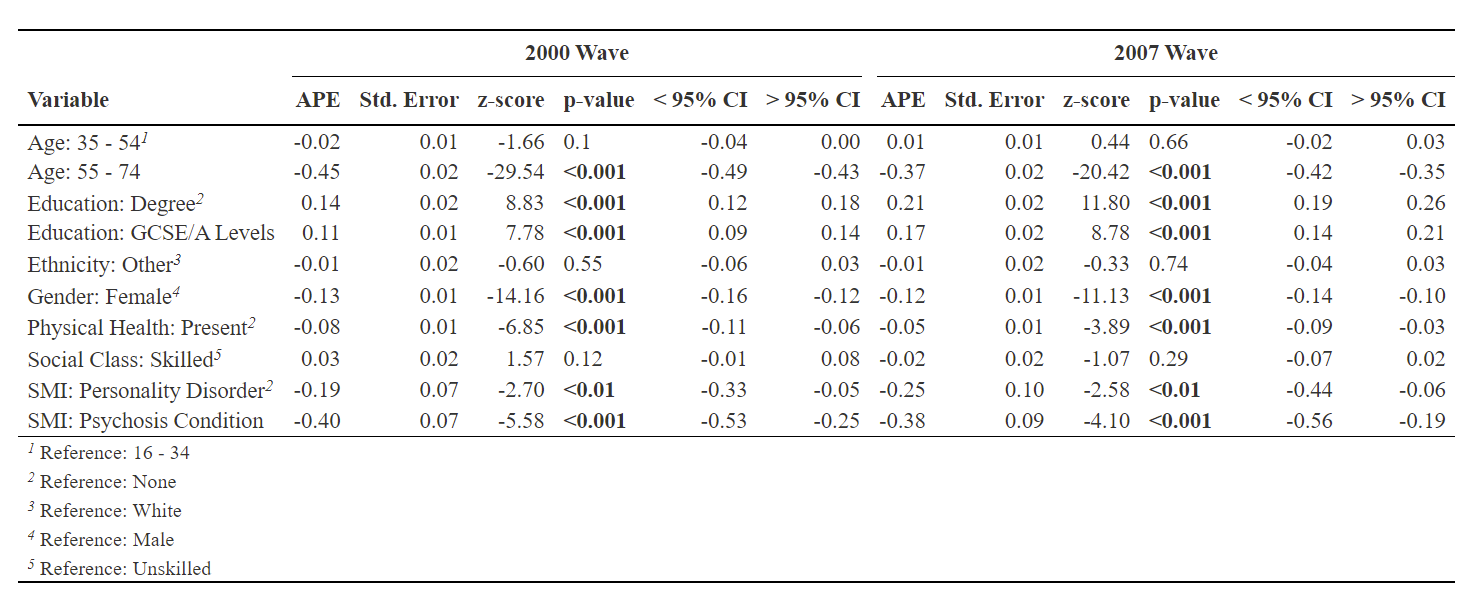
\includegraphics[width=450px,height=300px]{figure/apesmit} \caption[Average Partial Effects for SMI Type]{Average Partial Effects for SMI Type in 2000 and 2007}\label{fig:apesmit}
\end{figure}



\begin{figure}
\includegraphics[width=450px,height=300px]{figure/apesmitp} \caption[Average Partial Effects Plot for SMI Type]{Average Partial Effects Plot for SMI Type in 2000 and 2007}\label{fig:apesmitp}
\end{figure}
\hypertarget{goodness-of-fit-for-type-of-severe-mental-illness}{%
\subsection{Goodness of Fit for Type of Severe Mental Illness}\label{goodness-of-fit-for-type-of-severe-mental-illness}}

The results of the diagnostic tests for the models ran on severe mental illness type and economic activity are detailed in FIgure \ref{fig:gofsmit}. McFadden's pseudo R2 statistic ranged from 0.28 for the model applied to the 2000 survey wave to 0.24 for the model applied to 2007 survey wave. These showed the models to be of excellent fit, with a small decrease in fit for the 2007 survey wave model.




\begin{figure}
\includegraphics[width=460px,height=100px]{figure/gofsmit} \caption[Goodness of Fit for SMI Type Models]{Goodness of Fit for SMI Type Models in 2000 and 2007}\label{fig:gofsmit}
\end{figure}
\hypertarget{summary-3}{%
\section{Summary}\label{summary-3}}

The relationships between both common mental disorders and severe mental illnesses and economic activity were examined using data from two survey waves in 2000 and 2007. Logistic regression models were applied to each year to determine the odds of being economically active or employed while controlling for demographic, health, and educational factors.

In Section 6.3, the focus was on the influence of common mental health disorders and severe mental illness on economic activity. Results showed that having a common mental health disorders or severe mental illness was negatively associated with employment and that this association was statistically significant in both survey waves. The negative effect of severe mental illness was greater than for common mental health disorders, as expected. The negative effect of common mental health disorders on economic activity was found to be stronger in the 2007 survey wave than in 2000.

In Section 6.4, the focus shifted to the impact of treatment use for common mental health disorders on employment outcomes. Results showed that treatment use, including the use of mental health services and medication, was negatively associated with employment. However, the effect of using counselling services alone on employment was not statistically significant in the 2007 survey wave.

In Section 6.5, the focus shifted to the impact of specific types of common mental health disorders on economic activity. Results showed that all types of common mental health disorders were associated with a decreased likelihood of being economically active, with depression, generalised anxiety and depression, and mixed anxiety and depression being statistically significant in the 2000 survey.

In Section 6.6, the focus shifted to the impact of treatment use for severe mental illness on employment outcomes. Results showed that being in treatment and having both medication and counselling was the next largest negative effect on economic activity, at 25\% in 2000 and 30\% in 2007. Being female and having used any form of mental health service also had a negative effect on economic activity.

In Section 6.7, the focus shifted to the impact of specific types of severe mental illness on economic activity. Results showed that both having a psychosis condition or personality disorder were both highly statistically significant and negatively associated with economic activity, with psychosis being more statistically significant than personality disorders in both the 2000 and 2007 survey waves.

The large negative APE values for the age group 55 to 74 seen in several models should be interpreted in the light that individuals of this age made up 25\% and 28\% of the whole sample in the 2000 and 2007 survey waves. Education had a significant positive effect on economic activity, with those who have gained a degree being more likely to be economically active, and those with GCSE's or A Levels following. Education was consistently one of the largest positive APE across models but represented 22\% and 30\% of the overall samples in the 2000 and 2007 survey waves. Gaining GCSEs and A Levels also had a positive effect and represented 51\% and 47\% of the sample in the 2000 and 2007 wave. Social class and age can also play a role in economic activity, although the impact of these factors may vary depending on the economic conditions and the state of the labour market at a given time. Factors that have a negative effect on economic activity include being aged between 55 and 74 years old and being female.

Results have shown that people with mental illnesses are less likely to be employed, which could lead to increased poverty, stigma and difficulty functioning within society. Therefore, it is crucial for society to invest in holistic policies and programs that support individuals with mental illnesses in finding and keeping employment. It is important to note that these findings may be influenced by changes in the prevalence of these conditions within the population and changes in the way that they are diagnosed and treated. Also that the sample size for severe mental illness was small, and also possible that the sample may not be representative of the larger population, which could lead to bias in the results, and means that the findings of the study should be taken with caution due to the possibility of a lack of representativeness and statistical power.

Furthermore, the study's findings also reveal the need for a more comprehensive approach to mental health support, as opposed to solely focusing on medication and counselling. The negative effects of treatment use on employment outcomes suggest that while these may be necessary due to condition severity, they are not sufficient in addressing the barriers to employment faced by individuals with common mental health disorders or severe mental illness. This includes addressing the access to education and training opportunities, address discrimination and bias, and provide affordable housing and social support can help to break the cycle of poverty and unemployment for individuals with mental illnesses. Additionally, policies that aim to reduce the stigma around mental illness and promote awareness can help to increase the likelihood of individuals with mental illnesses seeking treatment and support.

In conclusion, this study found that common mental disorders and severe mental illnesses have a negative impact on economic activity. The use of health services or treatments for mental illness, as well as the specific types of mental illness, were found to have a significant negative effect on the likelihood of being active. Demographic factors such as age, gender, and physical health conditions were also found to have a negative effect on employment outcomes. Education was found to be positively associated with economic activity. These results highlight the need for effective treatment and support for individuals with mental illness, as well as addressing societal stigmas surrounding mental health, to promote better economic outcomes for individuals with mental illness.

\hypertarget{chapter7}{%
\chapter{Discussion}\label{chapter7}}

\hypertarget{chapter-overview-6}{%
\section{Chapter Overview}\label{chapter-overview-6}}

This chapter discusses key findings from this thesis and places their implications in context. A section comparing findings to previous research is then presented before a section outlining the general strengths and limitations of the thesis. The final section outlines recommendations for future research. Concluding statements can be found in Chapter \ref{chapter8}.

\hypertarget{findings-in-context}{%
\section{Findings in Context}\label{findings-in-context}}

This section summarises the key findings, relates them to existing literature and draws out implications for policy. There are four subsections covering: 1. The role of demographic factors in economic activity, 2. the impact of common mental health disorders and severe mental illness on economic activity, 3. the effect of treatment use on economic activity, and 4. the influence of common mental health disorders and severe mental illness type on economic activity.

This work highlights the significant impact that demographic factors, particularly age, gender, and education, have on economic activity in England, particularly in the context of poor mental health. The findings suggest that older individuals and women are more likely to face barriers to employment, and that education has a positive impact on economic activity. To address these issues, it is crucial for society to invest in holistic policies and programs that support individuals with mental illnesses in finding and keeping employment if able, addressing the barriers faced by older individuals and women, and providing support and resources that are tailored to their specific needs. Additionally, it is important to invest in education and training programs that support individuals in gaining the skills and qualifications needed to access employment opportunities, and to address the broader social context, including the prevalence of mental health conditions, the type and source of support and resources, and the level of stigma and discrimination faced by individuals living with mental illnesses.

\hypertarget{demographic-factors-and-economic-activity}{%
\subsection{Demographic Factors and Economic Activity}\label{demographic-factors-and-economic-activity}}

The impact of demographic factors on economic activity is a topic that has been widely researched in recent years, particularly in relation to poor mental health and employment. In the UK, the relationship between demographic factors and economic activity is shaped by various social, economic, and political factors, including changes in the labour market, the prevalence of certain mental health conditions, and the availability of support and resources for individuals with common mental health disorders or severe mental illness in particular (\protect\hyperlink{ref-RN2247}{Dobbins and Plows, 2022}).

The data from the 2000 and 2007 waves of the Adult Psychiatric Morbidity Survey (APMS) suggests that demographic factors such as age, gender, and education have a significant impact on economic activity in England. Individuals aged 55 to 74 were less likely to be economically active, with a negative probability of activity in the 2000 and 2007 survey wave. Similarly, being female was also negatively associated with economic activity in both survey waves. The work by Ralston and Formby (\protect\hyperlink{ref-RN4822}{Ralston and Formby, 2020}) also highlights the significant changes in the occupational position of young people in the UK following the Great Recession. These changes in occupational position, particularly the disproportionate loss of less advantaged occupations for young men and more advantaged occupations for young women, have important implications for mental health outcomes. As research has shown, socioeconomic disadvantage, including unemployment and low income, is associated with poorer mental health outcomes, these shifts in occupational position may be contributing to increased mental health disparities and inequality in the UK, highlighting the need for policies and programs to support young people in finding and maintaining employment.

These findings align with previous research which has demonstrated that older individuals and women are more likely to face different choices and barriers to employment, particularly when they are living with poor mental health. For example, a study by the Royal College of Psychiatrists (\protect\hyperlink{ref-RN371}{Modini \emph{et al.}, 2016}) found that older individuals with mental health conditions are more likely to experience discrimination in the workplace and face barriers to returning to work after a period of absence. Similarly, research by the TUC has shown that women with mental health conditions are more likely to experience discrimination in the workplace and face barriers to progression and career development.

On the other hand, the current work found that education was positively associated with economic activity, with those who have gained a degree the most likely to be economically active. Similarly, those with GCSEs or A Levels also had a positive effect on economic activity, a second to having gained a degree. This is in line with research by the Centre for Mental Health (\protect\hyperlink{ref-RN2349}{McGrath, Griffin and Mundy, 2016}) which found that individuals with higher levels of education are more likely to be economically active and to have better employment outcomes. Furthermore, research by the Mental Health Foundation (\protect\hyperlink{ref-RN2375}{Sabella, 2021}) found that individuals with higher levels of education are more likely to have better mental health outcomes and less likely to experience discrimination in the workplace.

It is important to note that the relationship between demographic factors and economic activity is complex and shaped by a number of social, cultural, economic, and political factors (\protect\hyperlink{ref-RN2246}{Taylor \emph{et al.}, 2017}). For instance, changes in the labour market and the availability of support and resources for individuals with mental illnesses can impact the relationship between different demographic factors and economic activity. Furthermore, the relationship between demographic factors and economic activity is also shaped by the broader social context, including the prevalence of mental health conditions, the type and source of support and resources, and the level of stigma and discrimination faced by individuals living with mental illnesses.

Overall, the data analysed in this work highlights the significant impact that demographic factors have on economic activity in England, particularly in the context of poor mental health. The findings suggest that older individuals and women are more likely to face barriers to employment and that education has a positive impact on economic activity. These findings show that it is crucial for society to invest in holistic policies and programs that support individuals with mental illnesses in finding and keeping employment if able to. This includes addressing the barriers faced by older individuals and women and providing support and resources that are tailored to their specific needs (\protect\hyperlink{ref-RN208}{Rinaldi \emph{et al.}, 2010}). Additionally, it is important to invest in education and training programs that support individuals in gaining the skills and qualifications needed to access employment opportunities (\protect\hyperlink{ref-RN4734}{Pilling, 2022}). Furthermore, addressing the social determinants of mental health such as poverty, housing, and discrimination will play a crucial role in improving the economic activity of individuals living with common mental health disorders and severe mental illness long term (\protect\hyperlink{ref-RN2236}{Recovery in the Bin, 2022}).

To give one example, the Westminster government implemented the New Deal for Disabled People in 2001, which aimed to support individuals with disabilities in finding and maintaining employment. Additionally, the introduction of the Disability Discrimination Act, implemented in 1995, aimed to prevent discrimination against individuals with disabilities in the workplace. These policies were in place during the time period in which the data from the APMS was collected and would have likely had an impact on the relationship between the demographic factors and economic activity. Furthermore, it is also important to consider the broader social and economic context of the time, such as changes in the labour market and the availability of support and resources for individuals with mental illnesses.

One specific example of a policy response that was implemented between 2000 and 2007 that aimed to address the barriers faced by older women in the workforce was the ``Women and Work Commission'' established in 2006. The Commission aimed to address the issues faced by women in the workplace, including discrimination, lack of flexible working options, and the gender pay gap. The Commission also focused on addressing the specific challenges faced by older women, such as age discrimination and lack of opportunities for career development. One of the key recommendations from the Commission was to increase the availability of flexible working options for older women, in order to enable them to continue working while balancing care giving responsibilities. Additionally, the Commission recommended initiatives to tackle age discrimination in the workplace and increase opportunities for older women to access training and development programs. This policy aimed to improve the economic activity of older women in the UK, by addressing the barriers they faced in the workforce.

\hypertarget{the-impact-of-common-mental-health-disorders-and-severe-mental-illness-on-economic-activity}{%
\subsection{The Impact of Common Mental Health Disorders and Severe Mental Illness on Economic Activity}\label{the-impact-of-common-mental-health-disorders-and-severe-mental-illness-on-economic-activity}}

We explored the relationship between common mental health disorders and severe mental illness, and economic activity using data from the two survey waves. The social context of the UK between 2000 and 2007 was marked by a shift towards a more flexible labour market, where individuals with common mental health disorders and severe mental illness may have been at a disadvantage in terms of finding and maintaining employment.

As expected, the results indicate that having a common mental health disorders or severe mental illness was negatively associated with employment and that this association was statistically significant in both survey waves. The negative effect of common mental health disorders on economic activity was found to be stronger in the 2007 survey wave. This negative association between common mental health disorders and severe mental illness and economic activity is consistent with previous research, which has shown that individuals with mental health conditions are more likely to experience economic inactivity, unemployment, and reduced income (\protect\hyperlink{ref-RN4812}{Kromydas \emph{et al.}, 2021}). This is particularly concerning given that poverty and social exclusion are known risk factors for mental health problems since it creates the risk of a downward spiral where mental health problems lead to a reduction in income which in turn increases the risk of such problems.

It is important to note that the negative association between common mental health disorders and severe mental illness and economic activity may be influenced by a number of factors, including the availability of treatment and support, the attitudes of employers and colleagues, and the nature of the work itself. For example, research has shown that individuals with common mental health disorders and severe mental illness are more likely to experience discrimination and stigma in the workplace (\protect\hyperlink{ref-RN441}{Hansen, Bourgois and Drucker, 2014}). This can make it difficult for them to find and maintain employment, even when they have the necessary qualifications and skills (\protect\hyperlink{ref-RN2252}{Bouwmans \emph{et al.}, 2015}).

These findings show the need for support for individuals with common mental health disorders and severe mental illness in finding and maintaining employment (\protect\hyperlink{ref-RN2236}{Recovery in the Bin, 2022}). This includes not just providing access to treatment and support, but also addressing the structural and societal factors that contribute to the marginalization and disadvantage of individuals with mental health conditions. One key area is in reducing poverty and social exclusion, as these factors have been shown to have a significant impact on mental health outcomes and can exacerbate the challenges faced by individuals with common mental health disorders and severe mental illness in the workforce. Additionally, promoting positive attitudes towards mental health in the workplace and creating more inclusive and flexible working environments can help to address the discrimination and stigmatization that individuals with mental health conditions often face (\protect\hyperlink{ref-RN4734}{Pilling, 2022}).

It is also important to note that these findings may be influenced by changes in the prevalence of these conditions within the population and changes in the way that they are diagnosed and treated. However, it is clear that there is a need for further research to better understand the specific challenges faced by individuals with common mental health disorders and severe mental illness in the workplace, as well as the most effective strategies for supporting them, given the significant impact that common mental health disorders and severe mental illness can have on an individual's ability to participate in the workforce. Furthermore, it is important to recognize that mental health is a social determinant of health and should be addressed holistically by addressing the societal and structural factors that contribute to mental health disparities.

\hypertarget{effects-of-treatment-and-service-use-on-economic-activity}{%
\subsection{Effects of Treatment and Service Use on Economic Activity}\label{effects-of-treatment-and-service-use-on-economic-activity}}

The effects of treatment or service use on economic activity are a key consideration when examining the relationship between mental health and employment. We may hope that effective treatment or services might increase the changes of those with common mental health disorders or severe mental illness finding or remaining in employment. In practice, the results indicate that treatment and service use are negatively associated with economic activity and indicate illness severity. These findings are consistent with previous research, which suggests that individuals with mental health conditions who receive treatment are more likely to be unemployed or inactive (\protect\hyperlink{ref-RN175}{Waddell and Burton, 2006}). These results should not be interpreted as indicating that treatments or services are not effective. Rather they indicate that those receiving treatments or using services are likely to experience more severe mental health challenges. To judge the impacts or benefits of treatments and services, we would need a different research design.

When we control treatment and service use, we still see significant negative relationships between common mental health disorders and severe mental illness, and economic activity. This suggests that even the `less unwell' with these conditions still suffer significant disadvantage in the labour market. This is a crucial insight, as it highlights the need for wider access to treatment and support services for individuals with common mental health disorders and severe mental illness, even those who are considered to be \emph{``less unwell''}. It suggests that even those who do not currently receive these kinds of services still face significant disadvantages in the labour market. This highlights the importance of addressing the root causes of these conditions, rather than simply treating the symptoms. Additionally, it emphasizes the need for more comprehensive support services that can help individuals with common mental health disorders and severe mental illness to manage their symptoms and maintain employment. This may include mental health services, job training and placement programs, and other social support services that can help to reduce the negative impact of these conditions on economic activity (\protect\hyperlink{ref-RN2235}{Johnson, 2021}).

However, the results also showed that the using counselling services alone on employment was not statistically associated with lower economic activity in the 2007 survey wave. The lack of a significant relationship between counselling and economic activity suggests that counselling is the treatment that individuals who are least unwell tend to use. This highlights the need for more tailored treatment and support services that can effectively address the specific needs of individuals with common mental health disorders and severe mental illness, regardless of their level of illness. It also suggests that more research is needed to better understand the underlying causes of these conditions and how they impact economic activity.

Individuals with personality disorders, such as borderline personality disorder, may struggle with managing their emotions and behaviours in a workplace setting. Counselling services may be able to address these issues but may not be able to provide the additional support and accommodation that these individuals may need in order to be successful in a work environment. Research has shown that individuals with severe mental illnesses often have multiple, complex needs that require a coordinated, multidisciplinary approach to treatment and support. This may include not just counselling services, but also employment support, housing support, and other services (\protect\hyperlink{ref-RN175}{Waddell and Burton, 2006}). Limited access to counselling services in the community and lack of continuity of care may also be a barrier for individuals with severe mental illnesses in finding and maintaining employment. A lack of employment support services specifically tailored to individuals with severe mental illnesses may also play a role in the limited effectiveness of counselling services alone in supporting employment (\protect\hyperlink{ref-RN2254}{Juurlink \emph{et al.}, 2022}).

This highlights the intersectionality of gender and mental health in determining employment outcomes and the need for gender-sensitive policies and programs to support individuals with mental health conditions in finding and maintaining employment (\protect\hyperlink{ref-RN2369}{Sansone and Sansone, 2011}). This includes developing and implementing gender-sensitive mental health services, such as specialized counselling and support groups, targeted job training and placement services for women with mental health conditions to increase their employability and job retention. Offering flexible work arrangements, such as part-time or telecommuting options to accommodate their needs and support their recovery. Offering accommodation in the workplace, such as mental health days and mental health leave are initiatives that could also impact positively keeping people with common mental health disorders and severe mental illness in employment. Providing education and awareness campaigns for employers should also positively impact, increasing understanding of mental health conditions and reducing the discrimination and stigma experienced by those living with mental health conditions in the workplace. Offering inclusive parenting support services for caregivers with mental health conditions, such as counselling, support groups, and respite care, to help them manage their condition and continue to provide for their children (\protect\hyperlink{ref-RN2321}{Jenkins, 2018}).

Moreover, the results of this study indicate that the negative effect of common mental health disorders and severe mental illness on economic activity is statistically significant in both survey waves. This is further evidence that individuals with mental health conditions face significant barriers in finding and maintaining employment. These findings have important implications and highlight the need for policies and programs that address the social determinants of mental health, such as poverty and unemployment, and support individuals with mental health conditions in finding and maintaining employment. This includes providing access to comprehensive, evidence-based treatment, including counselling and medication, as well as employment support services, such as job coaching and vocational rehabilitation (\protect\hyperlink{ref-RN4746}{Rizza and Fioritti, 2020}).

Additionally, the results also highlight the need for policies and programs that address the intersectionality of mental health, gender and socioeconomic status, and support individuals with mental health conditions in navigating the changes in the labour market and finding and maintaining employment. This includes addressing the structural barriers that individuals with mental health conditions face in finding and maintaining employment, such as discrimination and stigma, and providing targeted support for marginalized groups, such as women and ethnic minorities (\protect\hyperlink{ref-RN3434}{Eads \emph{et al.}, 2021}).

\hypertarget{the-influence-of-common-mental-health-disorders-and-severe-mental-illness-type-on-economic-activity}{%
\subsection{The Influence of Common Mental Health Disorders and Severe Mental Illness Type on Economic Activity}\label{the-influence-of-common-mental-health-disorders-and-severe-mental-illness-type-on-economic-activity}}

In this section, we explored the influence of specific types of common mental disorders and severe mental illnesses on economic activity between 2000 and 2007. Using logistic regression models, we analysed the odds of being economically active while controlling for demographic, health, and educational factors.
One of the key findings in this section was the negative association between specific types of common mental health disorders and economic activity. Results showed that all types of common mental health disorders were associated with a decreased likelihood of being economically active, with depression, generalised anxiety and depression, and mixed anxiety and depression being statistically significant in the 2000 survey. These findings align with previous research that has found individuals with depression to be at an increased risk of inactivity and unemployment (\protect\hyperlink{ref-RN4813}{Hakulinen \emph{et al.}, 2016}).

Studies have found that individuals with depression have an increased risk of inactivity and unemployment (\protect\hyperlink{ref-RN4813}{Hakulinen \emph{et al.}, 2016}). They may have difficulty with motivation, concentration, and energy levels, which can make it hard to carry out daily tasks. They may also experience social withdrawal and isolation, which can further affect their ability to work. Anxiety disorders, such as generalised anxiety disorder (GAD) and social anxiety disorder (SAD), are associated with increased risk of unemployment and reduced productivity at work (\protect\hyperlink{ref-RN4814}{Kaltenthaler, Pandor and Wong, 2014}). Individuals with GAD may have difficulty with excessive worrying, which can affect their ability to focus and make decisions, while individuals with SAD may have difficulty interacting with others and may avoid social situations, which can make it hard to hold down a job. Individuals with OCD may have difficulty with work performance and career progression due to the time-consuming nature of their compulsions, which can make it hard to meet job demands (\protect\hyperlink{ref-RN4815}{Mohammad \emph{et al.}, 2022}). They may also experience social isolation and difficulty forming relationships, which can further affect their ability to work. Studies have found that individuals with panic disorder may have difficulty functioning in the workplace due to the sudden onset of panic attacks and the associated symptoms such as shortness of breath, heart palpitations, and feelings of impending doom (\protect\hyperlink{ref-RN4816}{Curtiss \emph{et al.}, 2021}). They may also experience social isolation and difficulty forming relationships, which can further affect their ability to work.

Another key finding was the negative association between specific types of severe mental illness and economic activity. Results showed that both having a psychosis condition or personality disorder were both highly statistically significant and negatively associated with economic activity, with psychosis being more statistically significant than personality disorders in both the 2000 and 2007 survey waves. These findings are consistent with previous studies that have found individuals with psychosis to be at a higher risk of economic inactivity (\protect\hyperlink{ref-RN3505}{Shemtob and Mujong, 2021}).

These findings on the influence of specific common mental health disorders and severe mental illness types on economic activity are particularly concerning for those individuals living with psychosis and personality disorder. Results show that both having a psychosis condition, or a personality disorder were both highly statistically significant and negatively associated with economic activity, with psychosis being more statistically significant than borderline personality disorder in both the 2000 and 2007 survey waves. This highlights the need for specific and targeted support for individuals living with these conditions in order to promote equality in the workforce and beyond (\protect\hyperlink{ref-RN2236}{Recovery in the Bin, 2022}).

Individuals living with psychosis may be less likely to be economically active for a variety of reasons, such as symptoms of their condition such as hallucinations, delusions, and disorganized thinking, which can make it difficult for an individual living with the condition to function in a workplace setting. This can lead to increased poverty, stigma, and difficulty functioning within society, which highlights the importance of investing in policies and programs that support individuals with psychosis in finding and keeping employment (\protect\hyperlink{ref-RN4716}{Watts, 2019}).

Similarly, individuals living with personality disorder may face challenges in finding and maintaining employment due to their condition. They may face difficulties in managing their emotions and behaviors in a workplace setting, which can lead to discrimination, prejudice, and negative stereotypes. This highlights the need for mental health awareness, education, and inclusion in workplaces, along with providing appropriate treatment and support for individuals living with personality disorders (\protect\hyperlink{ref-RN4736}{Schäfer and Fisher, 2022}).

This has highlighted the significant difficulties faced by individuals living with common mental health disorders and severe mental illness in the UK in terms of their economic activity. The findings show that specific types of common mental health disorders and severe mental illness, such as depression and psychosis, are associated with a decreased likelihood of being economically active. This is particularly concerning for individuals living with psychosis and personality disorder, who are at a higher risk of economic inactivity and face unique challenges in the workforce. These findings underscore the need for targeted and specific support for individuals living with common mental health disorders and severe mental illness, including addressing societal and structural factors that contribute to mental health disparities and promoting mental health awareness and inclusion in the workplace. It is crucial that society invests in policies and programs that support individuals with common mental health disorders and severe mental illness in finding and keeping employment, in order to promote equality and inclusion for all (\protect\hyperlink{ref-RN2334}{Bentall, 2003}).

\hypertarget{comparisons-to-previous-research-and-contribution}{%
\section{Comparisons to Previous Research and Contribution}\label{comparisons-to-previous-research-and-contribution}}

This study is unique in its focus on the specific relationship between common mental disorders and severe mental illnesses and their impact on economic activity. Previous research has primarily examined the effect of mental illness on employment outcomes but has not delved into the specific types of common mental health disorders and severe mental illness that may have a greater impact. It draws on two national cross-sectional surveys of the general population.

This study found that all types of common mental health disorders were associated with a decreased likelihood of being economically active: with depression; generalised anxiety and depression; and mixed anxiety and depression being statistically significant in the 2000 survey. Additionally, both psychosis conditions and personality disorders were found to be highly statistically significant and negatively associated with economic activity, with psychosis having a greater impact. These findings add to the growing body of literature that highlights the detrimental effect of mental illness on economic activity and the importance of targeted interventions and support for individuals with specific types of common mental health disorders and severe mental illness.

Previous research on the relationship between common mental health disorders and severe mental illness and economic activity has primarily focused on the overall impact of these conditions. This study, however, aimed to specifically examine the influence of specific types of common mental health disorders and severe mental illness on economic activity. The findings of this study support previous research that has shown a negative relationship between common mental health disorders and severe mental illness and economic activity but adds new insight by highlighting the particularly strong negative impact of psychosis and borderline personality disorder on economic activity. These findings contribute to a growing body of research that suggests a need for policies and programs that support individuals with common mental health disorders and severe mental illness in finding and maintaining employment, with a focus on addressing the specific challenges faced by individuals with psychosis and borderline personality disorder. The study used logistic regression models to examine the odds of being employed while controlling for demographic, health, and educational factors.

One key finding of the study is that individuals with common mental health disorders and severe mental illness were less likely to be employed, highlighting the need for better support and policies to help individuals with these conditions find and keep employment. The study also found that treatment use, including the use of mental health services and medication, was negatively associated with employment. Additionally, the study found that specific types of common mental health disorders, such as depression, generalised anxiety and depression, and mixed anxiety and depression, were statistically significant in negatively impacting economic activity.

In comparison to previous research, this study adds to the understanding of the specific challenges faced by individuals with common mental health disorders and severe mental illness in the workplace and the most effective strategies for supporting them. The study also highlights the need for further research to better understand the relationship between specific conditions and economic activity. Additionally, the study's use of data from multiple survey waves and a nationally representative sample allows for a more comprehensive understanding of the relationship between common mental health disorders, severe mental illness and economic activity over time. The study's findings are important for informing policy and practice in the UK and beyond to promote social justice and equality for individuals with common mental health disorders and severe mental illness.

Furthermore, it also examined the impact of specific types of common mental health disorders and severe mental illness on economic activity. The study found that all types of common mental health disorders were associated with a decreased likelihood of being economically active, with depression, generalised anxiety and depression, and mixed anxiety and depression being statistically significant in the 2000 survey. Additionally, the study found that both having a psychosis condition or personality disorder were both highly statistically significant and negatively associated with economic activity, with psychosis being more statistically significant than personality disorders in both the 2000 and 2007 survey waves. These findings are important as they contribute to the understanding of the specific challenges faced by individuals with common mental health disorders and severe mental illness in the workplace and the most effective strategies for supporting them.

This study, which focuses on the relationship between common mental disorders and severe mental illnesses and their impact on economic activity, adds to the body of research by using data from two survey waves in 2000 and 2007, applying logistic regression models to determine the odds of being employed while controlling for demographic, health, and educational factors. This allows for a more comprehensive understanding of the relationship between common mental health disorders and severe mental illness and economic activity. Additionally, this study also examines the impact of treatment use on employment outcomes, providing insight into the effectiveness of different forms of treatment in supporting individuals with common mental health disorders and severe mental illness in the workforce. The findings of this study are important as they reveal the significant negative impact that common mental health disorders and severe mental illness can have on an individual's ability to participate in the workforce, highlighting the need for more attention and support for individuals with these conditions in order to promote social justice and equality. This study is also important as it provides a more detailed view of the specific challenges faced by individuals with different types of common mental health disorders and severe mental illness in the workforce, and the most effective strategies for supporting them.

The work adds to the existing body of research on the relationship between common mental disorders and severe mental illnesses and their impact on economic activity. These findings are important in comparison to previous research, as they provide a comprehensive understanding of the negative impact that common mental health disorders and severe mental illness can have on an individual's ability to participate in the workforce and highlight the need for more attention to be paid to this issue in order to promote social justice and equality in the UK.

The use of logistic regression models in this study to examine the relationship between common mental disorders and severe mental illnesses and economic activity, as well as the influence of treatment use on employment outcomes, adds to the growing body of research on the topic. The results of this study, which used data from two survey waves in 2000 and 2007, showed that having a common mental health disorders or severe mental illness was negatively associated with employment and that this association was statistically significant in both survey waves. The negative effect of common mental health disorders on economic activity was found to be stronger in the 2007 survey wave. Additionally, treatment use, including the use of mental health services and medication, was negatively associated with employment. These findings provide important insights into the challenges faced by individuals with common mental health disorders and severe mental illness in the workforce and the potential strategies for supporting them.

It is worth noting that previous research on the impact of common mental disorders and severe mental illnesses on economic activity has used a variety of methodologies. For example, some studies have used data from the Adult Psychiatric Morbidity Survey (APMS) to examine the relationship between mental health and employment, while others have used data from other sources. Despite these differences, the findings of this study are consistent with those of previous research in showing that individuals with common mental health disorders and severe mental illness are less likely to be economically active than those without these conditions. Additionally, the use of logistic regression models in this study allows for a more detailed examination of the relationship between mental health and employment, controlling for demographic, health, and educational factors. These findings are important as they highlight the need for better support and policies for individuals with common mental health disorders and severe mental illness in the workforce.

Overall, this study contributes to a growing body of literature that highlights the detrimental effect of mental illness on economic activity and the importance of targeted interventions and support for individuals with specific types of common mental health disorders and severe mental illness. It builds on previous research by specifically examining the influence of different types of common mental health disorders and severe mental illness on economic activity, rather than simply focusing on the overall impact of these conditions. The study's use of data from multiple survey waves and a nationally representative sample allows for a more comprehensive understanding of the relationship between common mental health disorders, severe mental illness and economic activity over time.

One key finding of the study is that individuals with common mental health disorders and severe mental illness were less likely to be employed, highlighting the need for better support and policies to help individuals with these conditions find and keep employment. The study also found that treatment use, including the use of mental health services and medication, was negatively associated with employment. Additionally, the study found that specific types of common mental health disorders, such as depression, generalised anxiety and depression, and mixed anxiety and depression, were statistically significant in negatively impacting economic activity.

The study's findings are important for informing policy and practice in the UK and beyond to promote social justice and equality for individuals, particularly those experiencing multiple and place-based disadvantages associated with decades of de-industrialisation and the degradation of working-class employment opportunities. The belief in the concepts of generations and cultures of worklessness as improperly held and it is time they are done away with (\protect\hyperlink{ref-RN4820}{Ralston and Gayle, 2017}). This will help to dispel the myths and stereotypes that have been used to demonise individuals, particularly those with severe mental illness, and instead focus on addressing the root causes of poverty and inequality. This works results suggest that there is a need for policies and programs that support individuals with common mental health disorders and severe mental illness in finding and maintaining employment, with a focus on addressing the specific challenges faced by individuals with psychosis and borderline personality disorder.

Ralston's and collegues 2022 findings on the long-term impact of NEET status and the gendering of its outcomes highlights the importance of addressing the root causes of poverty and inequality for young people and emphasizes the gendered nature of work and labour from an early age that can follow into later life. It is clear that policies and programs need to be developed that support individuals, particularly those with severe mental illness, in finding and maintaining employment, to ensure that they have the opportunity to reach their full potential and participate fully in society (\protect\hyperlink{ref-RN4821}{Ralston \emph{et al.}, 2022}).

Furthermore, the study emphasizes the need for further research to better understand the relationship specific conditions and economic activity, in order to develop effective interventions and support programs for individuals with common mental health disorders and severe mental illness.

\hypertarget{strengths-and-limitations-of-this-work}{%
\section{Strengths and Limitations of This Work}\label{strengths-and-limitations-of-this-work}}

\hypertarget{strengths}{%
\subsection{Strengths}\label{strengths}}

The study utilizing the APMS data from 2000 and 2007 has several strengths that set it apart from other research that has used this same data. One strength of the study is its use of logistic regression models to determine the odds of being employed while controlling for demographic, health, and educational factors. This allows for a more accurate understanding of the specific relationship between common mental health disorders and severe mental illness and economic activity. Another strength is the use of data from two survey waves, in 2000 and 2007, which allows for an examination of the changes in the relationship between common mental health disorders and severe mental illness and economic activity over time. This allows for a more comprehensive understanding of how these factors have changed and how they may continue to change in the future.

Additionally, the study has a focus on treatment use and its effect on employment outcomes, which is an important aspect that has not been fully explored in previous research. We take treatment used to indicate more severe levels of mental ill health, enabling us to see how the `least unwell' do in the labour market. This highlights the need for further research and support in this area to help all individuals with common mental health disorders and severe mental illness find and maintain employment.

Furthermore, the study's use of a large and nationally representative sample allows for greater generalizability of its findings. In contrast, other studies that have used data from the APMS, such as those conducted by others may have had smaller sample sizes and did not consider, to the same extent, social context in their analysis. Overall, this study builds on previous research by providing a more detailed and nuanced understanding of the relationship between common mental health disorders and severe mental illness and economic activity in the UK.

Finally, the study also considers the social context of the UK between 2000 and 2007, which is an important consideration in understanding the specific challenges faced by individuals with common mental health disorders and severe mental illness in the workforce and how to promote social justice and equality in this area. Overall, the study provides valuable insights and adds to the body of research on common mental health disorders, severe mental illness, and economic activity, and its strengths, such as its critical social justice perspective and consideration of the social context of the UK, set it apart from other studies that have used data from the APMS. The detailed analysis and examination of specific conditions and demographic factors also adds a level of nuance and complexity to the understanding of the relationship between common mental health disorders, severe mental illness, and economic activity. Overall, this study makes an important contribution to the field and its findings should be taken into consideration in future research and policy decisions related to common mental health disorders, severe mental illness, and economic activity.

\hypertarget{limitations}{%
\subsection{Limitations}\label{limitations}}

The study used data from the Adult Psychiatric Morbidity Survey (APMS) to explore the relationship between common mental disorders and severe mental illness and economic activity in England between 2000 and 2007, has several limitations that should be considered when interpreting the results.

First, the study is limited by the cross-sectional design of the APMS, which does not allow for causality to be established. The study is only able to establish associations between common mental health disorders, severe mental illness and economic activity, and not the direction or mechanisms of these associations. Furthermore, the study is based on self-reported data, which may be subject to recall bias and social desirability bias.

Second, the study is limited by the measures used to assess common mental health disorders and severe mental illness and economic activity. The study used the Clinical Interview Schedule-Revised (CIS-R) to assess common mental health disorders and the Schedules for Clinical Assessment in Neuropsychiatry (SCAN) to assess severe mental illness. These measures have been validated for research purposes but may not capture the full range of symptoms and functional impairment associated with common mental health disorders and severe mental illness. Similarly, the study's measure of economic activity, which relied on self-reported employment status, may not properly capture other aspects of economic well-being, such as income and wealth.

Third, the study is limited by the sample used in the analysis. The study excluded individuals who were institutionalized, which could have led to an underestimation of the true prevalence of common mental health disorders and severe mental illness among these groups and the impact of these conditions on economic activity, especially when greater treatment use seems to indicate worse economic outcomes. The study also excluded individuals who were unable to speak English, which could have led to a bias in the sample. The survey also only recorded gender in a traditional binary, (named \texttt{sex} in the data, only recorded male and female) and fails to record non-binary or trans-identifying individuals. However, there is growing consensus that this has not stopped trans and non-binary individuals from appearing in survey data, only that previous methods have not captured this group adequately (\protect\hyperlink{ref-RN4817}{Doan, 2016}; \protect\hyperlink{ref-RN4818}{Sullivan, 2020}; \protect\hyperlink{ref-RN4819}{Guyan, 2022}).

Fourth, the study is limited by the lack of information on the specific types of common mental health disorders and severe mental illness, which may have different associations with economic activity. The study's focus on common mental health disorders and severe mental illness as broad categories may not capture the heterogeneity within these groups, which could have influenced the results.

One of the main limitations of this study is the small sample size of individuals reporting severe mental illness in both the 2000 and 2007 waves of the APMS. With only 46 and 56 individuals respectively, it is difficult to draw conclusions about the overall population of individuals with severe mental illness in relation to economic activity. The small sample size may lead to issues of sampling bias and limited statistical power, making it difficult to detect true relationships between severe mental illness and economic activity. Additionally, the small sample size may limit the generalizability of the study findings, as it may not accurately represent the experiences of individuals with severe mental illness in the broader population.

Furthermore, small sample size can also make it difficult to control confounding variables and ensure the robustness of the statistical analyses. Therefore, it is important to interpret the findings of this study with caution and to consider the limitations of the sample size when interpreting the results. It would be beneficial for future research to include a larger sample of individuals reporting severe mental illness to increase the generalizability of the findings. It is worth noting that the small sample size of this study may limit the generalizability of the findings to the wider population. This is a limitation that is consistent with other studies that have used data from the APMS, such as those conducted by previous research that used the data. These studies also had small sample sizes, which limited their ability to make generalizable conclusions about the population as a whole. Additionally, the small sample size in this study increases the likelihood of sampling error, which can lead to inaccurate or unreliable results. It is worth reflecting that the original plan of using administrative data may have overcome this limitation, and the barriers to using administrative data were beyond my control.
Moreover, the small sample size of this study can be a limitation when it comes to the ability to detect meaningful differences in the data. With a small sample size, any differences found in the data may not be statistically significant and may not be generalizable to the population as a whole. Furthermore, the small sample size of the severe mental illness group (46 and 56 in 2000 and 2007 respectively) specifically, may limit the ability to make conclusions about the specific population of individuals with severe mental illness. This is an important consideration given that the study aims to investigate the effect of common mental health disorders and severe mental illness on economic activity.

It is important to note that while the small sample size is a limitation of this study, it is a limitation that is common among studies that use data from the APMS. This is due to the nature of the survey, which is conducted on a representative sample of the population, rather than a comprehensive sample of the population. This means that while the sample size is small, it is still representative of the population as a whole. However, the small sample size should be considered when interpreting the results of this study and generalizing about the population.

Finally, the study is limited by the social context in which it was conducted. The study's data was collected between 2000 and 2007, which was a period of significant economic and political change in the UK, which could have influenced the results. The data itself cannot consider these changes and their potential impact on the relationship between common mental health disorders and severe mental illness and economic activity. It would also have improved the study to have had access to the APMS data for 2014. As well as providing a third wave of data, this would have extended the study period considerably, bringing in a time when the labour market suffered a significant deterioration after the Global Financial Crisis. However, the 2014 dataset of the APMS is still under a Special License Access agreement and could not be accessed in time to include it in this thesis.

In conclusion, the work provides important insights into the relationship between common mental health disorders and severe mental illness and economic activity in England between 2000 and 2007. However, the limitations of this works' methodology and sample must be considered when interpreting the results. These limitations highlight the need for further research to better understand the specific challenges faced by individuals living with common mental health disorders and severe mental illness in the workforce, and to explore the most effective strategies for supporting them. Given the significant impact that common mental health disorders and severe mental illness can have on an individual's ability to participate in the workforce, it is crucial that more attention is paid to this issue in order to promote social justice and equality in the UK and beyond.

\hypertarget{recommendations-for-future-research}{%
\section{Recommendations for Future Research}\label{recommendations-for-future-research}}

Based on the findings of this work, which used data from the Adult Psychiatric Morbidity Survey (APMS) to examine the relationship between common mental disorders, serious mental illness, and economic activity in England between 2000 and 2007, there are several key recommendations for future research in this area.

Firstly, it is recommended that future studies continue to use a critical social justice perspective when examining the relationship between common mental health disorders, severe mental illness, and economic activity. This study's focus on the social context of the UK between 2000 and 2007 is an important aspect that sets it apart from other studies and highlights the need to consider the broader social and structural factors that impact individuals with common mental health disorders and severe mental illness in the workforce.

Secondly, it is recommended that future studies find ways to access longitudinal data to examine changes in the relationship between common mental health disorders, severe mental illness, and economic activity over time. This study's use of data from two survey waves in 2000 and 2007 allows for some understanding of how these factors have changed and how they may continue to change in the future, but it is limited to not being able to track the same individuals over time. There may be scope to use linked administrative data to achieve this. This could also provide access to substantially greater sample sizes which could increase the level of detail which could be explored in the model. Future studies certainly need to consider using more robust data sources to increase sample size and generalizability of findings. The small sample size of 46 and 56 people reporting severe mental illness in 2000 and 2007, is a limitation of this study, and future studies should consider using more robust data sources to increase sample size and generalizability of findings.

Thirdly, it is recommended that future studies focus on specific types of common mental health disorders and severe mental illness to provide a more nuanced understanding of the relationship between mental health and economic activity. This study's focus on specific types of common mental health disorders and severe mental illness allows for a more accurate understanding of the specific challenges faced by individuals with different mental health conditions in the workforce.

Fourthly, it is recommended that future studies consider the use of mental health services and medication as a predictor of employment outcomes. This study's focus on the treatment use and its effect on employment outcomes is an important aspect that has not been fully explored in previous research and highlights the need for further research and support in this area to help individuals with common mental health disorders and severe mental illness find and maintain employment.

In addition to the recommendations for future research that have been previously discussed, there are several other areas that should be explored in order to further our understanding of the relationship between common mental health disorders, severe mental illness, and economic activity. One key area for future research is to examine the specific barriers and facilitators to employment for individuals with common mental health disorders and severe mental illness. This could include looking at the role of stigma and discrimination, as well as the impact of individual, organizational, and societal level factors on employment outcomes. Furthermore, research should also focus on understanding the role of different types of treatment and support in promoting employment for individuals with common mental health disorders and severe mental illness.

Another major area for future research is to examine the relationship between common mental health disorders, severe mental illness, and economic activity in other countries and cultural contexts. This would allow for a more comprehensive understanding of the global impact of common mental health disorders and severe mental illness on economic activity and would also provide valuable information for the development of cross-cultural policies and interventions. Additionally, future research should also examine the relationship between common mental health disorders, severe mental illness, and economic activity in different age groups and across the lifespan.

Finally, it is also important to consider the intersectionality of different demographic factors and how they may impact the relationship between common mental health disorders, severe mental illness, and economic activity. For example, research should examine the impact of race, ethnicity, and socioeconomic status on the relationship between common mental health disorders, severe mental illness, and economic activity, as well as the role of gender and gender identity, with more attention being paid to how we can accurately capture trans and non-binary individuals for example (\protect\hyperlink{ref-RN4819}{Guyan, 2022}) whether or not they already participate in survey data. By considering these intersectional factors, we can gain a more comprehensive understanding of the unique challenges faced by different groups of individuals with common mental health disorders and severe mental illness and how to promote social justice and equality in this area.

Overall, the study has provided valuable insights into the relationship between common mental health disorders, severe mental illness, and economic activity in England between 2000 and 2007. However, the limitations of the study, such as the small sample size and limited generalizability, must be taken into consideration when interpreting the findings. To build on the research conducted in this study, future research should focus on increasing sample size, incorporating a more diverse population, and utilizing more robust measures of common mental health disorders, severe mental illness, and economic activity. Additionally, future research should consider the role of social and economic policies in impacting the relationship between common mental health disorders, severe mental illness and economic activity, as well as the role of mental health support and treatment on employment outcomes. Furthermore, the research should also be done in other countries to see how the relationship between common mental health disorders, severe mental illness and economic activity varies across different cultures and contexts. By addressing these limitations and building on the strengths of this study, future research can provide a more comprehensive understanding of the relationship between common mental health disorders, severe mental illness, and economic activity, and inform policies and practices that promote social justice and equality for individuals with common mental health disorders and severe mental illness in the workforce.

\hypertarget{end}{%
\chapter*{End}\label{end}}
\addcontentsline{toc}{chapter}{End}

Every Wednesday since the start of 2018 I go to counselling. At first, I was resistant. I didn't know what I would talk about. I realised some things had maybe been bad growing up and leading to the start of my psychosis, but not that bad. At first, I thought it would fix me or at least make the voices go away like the medication promised to do. It did provide me with the first unfiltered space where I didn't have to mask emotions or the voices or how I felt.

It included everything and anything from childhood to doing this PhD. Sessions were often, and still are tearful. We've worked on imposter syndrome a lot over the years. I've laughed many times and said she must be dying for me to hand this thing in. In contrast with the many psychiatrists I've seen in ten minute slots over the years, she has not shied away from me, my life, and especially my lows. She was the first to not discharge me for non-compliance after disclosing self-harm and suicidal thoughts. Many times we've spoken about the people in the data used here. I've become emotional over the fact I have the chance to access counselling outside of the NHS and so many with SMI in the data don't. I thought I was weird for thinking this, she didn't. We've spoken about employment and SMI when I've voiced I don't feel like an anomaly, when the statistics say that I am. This was also refreshing as the only time a psychiatrist asked about my employment situation and I said I was doing a PhD, he was in such disbelief he goggled my supervisor to see if they were real. His words. He then turned round in his chair and said,
\begin{quote}
\emph{``You know people like you die 20 years
younger''.}
\end{quote}
We would talk a lot about family. This often left that horrible sinking feeling in my stomach. It felt like betraying them to talk about them in that way. The subject of counselling, much like doing the PhD, has only been discussed a few times. It Is something ``people like us don't do''. Despite hearing from others, especially neighbours on my mums street, that I must be doing so well, they're so proud of you, my family has, at times, expressed what I think is resentment at this PhD. I was the first to go to Uni in a family that places high value on \emph{``real''} employment -- this has never actually been defined, but does not include the PhD, being a lecturer or a researcher -- and children. On one hand they ask for advice and on the other they say I know nothing. And maybe I don't. Have they asked when I'll be finishing this work? Yes. Someone even asked for the title, but on being told, exclaimed,
\begin{quote}
\emph{``Oh no, no, no, Shell. That's too
depressing, you need to think positive
thoughts''.}
\end{quote}
\emph{(December 2022 -- taken from a longer reflexive piece)}

\hypertarget{chapter8}{%
\chapter{Conclusion}\label{chapter8}}

This work aimed to investigate the relationship between common mental disorders, severe mental illness, and economic activity in England. It provides a detailed understanding of the patterns of economic activity among individuals with common mental health disorders severe mental illness and how these vary by both individual and local labour market characteristics.

The APMS is a nationally representative survey of households in England that collects information on the prevalence and characteristics of mental health disorders in adults. The survey is conducted by the National Centre for Social Research (NatCen) and is commissioned by NHS Digital. The survey uses a face-to-face interview and a self-completion questionnaire to gather data on a range of mental health disorders, including common mental disorders such as depression and anxiety, and severe mental illness such as schizophrenia and bipolar disorder. The APMS also collects data on a range of socio-demographic characteristics, including age, gender, education, and employment status. The survey is conducted every seven years, with the most recent wave of data being collected in 2014. The APMS data is a valuable resource for researchers and policymakers as it provides a detailed understanding of the prevalence and characteristics of mental health disorders in the general population. It was a good choice for this work because it provides a comprehensive picture of the prevalence of mental health conditions in the general population and the factors associated with them, as well as its ease of access in light of working within the context of COVID-19. After data cleaning and restricting the samples to England only and capping the age at 74 to bring the 2000 and 2007 waves into line with each other, there were 7,247 individuals in the 2000 APMS survey wave, and 6,453 individuals in the 2007 survey wave.

Despite the increasing prevalence of poor mental health worldwide, work concentrating on severe mental illness in particular is less prevalent than work looking into common mental health disorders. Potential reason could be the complexity and diversity of severe mental illness, which can make it more difficult to study and understand in relation to employment. Additionally, there may be a lack of data on severe mental illness and employment due to the stigma and discrimination that individuals with severe mental illness often face, which can make it difficult for them to access and maintain employment. Furthermore, many individuals with severe mental illness may not be in the workforce, which can make it harder to collect data on their employment status. Finally, there may be fewer resources and funding streams dedicated to studying the relationship between severe mental illness and employment compared to common mental health disorders and employment, which can limit the amount of research conducted in this area. This all leads to a lack of good quality data available for analysis. The APMS study fills the gap in the current literature by providing detailed insights into the relationship between common mental disorders and severe mental illness and employment status in England. It provides a comprehensive understanding of how patterns of employment vary by individual and local labour market characteristics, and how this relationship has changed since 2000 in England.

The work also aimed to address the following research questions:
\begin{enumerate}
\def\labelenumi{\arabic{enumi}.}
\tightlist
\item
  How has the impact of common mental health disorders and severe mental illness on employment status changed since 2000 in England?
\item
  How do employment status patterns for individuals with common mental health disorders and severe mental illness compared to the rest of the population in England in 2007?
\item
  Is the relationship of severe mental illness to employment status different from the relationship of common mental health disorders to employment status in England?
\item
  How does living with common mental health disorders and severe mental illness affect the entrance of young adults (16-35 years old) to the labour force, in comparison to young adults without common mental health disorders and severe mental illness?
\item
  Are the effects of common mental health disorders and severe mental illness on employment status mitigated or exacerbated by other barriers or enablers, such as socioeconomic status, ethnicity, education, physical health, involvement in services?
\end{enumerate}
Results found that the impact of common mental health disorders and severe mental illness on employment status in England has changed since 2000 (RQ1). Specifically, the study found that there has been an increase in the number of individuals with common mental health disorders and severe mental illness who are unemployed or inactive in the labour market. Furthermore, the study found that the relationship between common mental health disorders and severe mental illness and employment status is complex and influenced by a number of demographic, social, and economic factors, including age, gender, education, and socioeconomic status. The study also found that the impact of common mental health disorders and severe mental illness on employment status is affected by changes in the labour market and the availability of support and resources for individuals with mental illnesses.

Findings showed that individuals with common mental disorders and severe mental illnesses were less likely to be employed compared to the rest of the population in England in 2007 (RQ2). Results from logistic regression models showed that having a common mental health disorders or severe mental illness was negatively associated with employment and that this association was statistically significant. Additionally, treatment used for common mental health disorders, including the use of mental health services and medication, was also found to negatively impact employment outcomes. Specific types of common mental health disorders and severe mental illness were also found to have a negative effect on economic activity, with psychosis conditions having a greater negative impact than personality disorders. Overall, the study highlights the need for society to invest in policies and programs that support individuals with mental illnesses in finding and keeping employment.

We also found that having a common mental disorder or severe mental illness was negatively associated with employment in both the 2000 and 2007 survey waves (RQ3). The study found that the negative effect of common mental health disorders on economic activity was stronger in the 2007 survey wave. The study also found that treatment use, including the use of mental health services and medication, was negatively associated with employment for individuals with common mental health disorders. However, the effect of using counseling services alone on employment was not statistically significant in the 2007 survey wave. Additionally, specific types of common mental health disorders and severe mental illness were found to have a negative impact on economic activity, with psychosis being more statistically significant than personality disorders in both survey waves. Overall, it appears that the relationship of severe mental illness on employment status is similar to the relationship of common mental health disorders on employment status in England (RQ1).

Results show that young adults living with common mental health disorders and severe mental illness were less likely to be employed and participate in the labour force, compared to their peers without mental health conditions (RQ4). The study used logistic regression models to examine the relationship between common mental health disorders and severe mental illness and economic activity while controlling for demographic, health, and educational factors. The results showed that having a common mental health disorders or severe mental illness was negatively associated with employment and that this association was statistically significant in both survey waves. Additionally, the study found that treatment use for common mental health disorders and severe mental illness also had a negative effect on employment outcomes. Overall, the study found that living with common mental health disorders and severe mental illness can have a significant impact on the entrance of young adults to the labour force.

We found that the effects of common mental disorders and severe mental illnesses on employment status are influenced by other factors such as socioeconomic status, ethnicity, education, physical health, and involvement in services (RQ5). Results from logistic regression models applied to the 2000 and 2007 survey waves showed that factors such as being female, having a physical health condition, being of older age, and having lower levels of education were negatively associated with employment. On the other hand, being skilled or having higher levels of education were positively associated with employment. Additionally, the study found that treatment used for common mental health disorders, including use of mental health services and medication, was negatively associated with employment. The study also found that certain types of common mental health disorders and severe mental illness were associated with a decreased likelihood of being economically active. Moreover, the study found that individual's socioeconomic status, ethnicity, education, physical health, and involvement in services can act as barriers or enablers that can mitigate or exacerbate the effects of common mental health disorders and severe mental illness on employment status.

In conclusion, the APMS study provides valuable insights into the relationship between common mental health disorders and severe mental illness and employment status in England. The study aimed to examine how the impact of common mental health disorders and severe mental illness on employment status has changed since 2000, to compare the employment status patterns of individuals with common mental health disorders and severe mental illness to the rest of the population in England in 2007, to determine if the relationship of severe mental illness on employment status is different from the relationship of common mental health disorders on employment status, and to explore how living with common mental health disorders and severe mental illness affects the entrance of young adults to the labour force. The study also highlights the importance of considering other barriers and enablers in addition to common mental health disorders and severe mental illness, such as socioeconomic status, ethnicity, education, physical health, and involvement in services.

The results of the study indicate that individuals with common mental health disorders and severe mental illness are less likely to be employed compared to the general population. The study also found that treatment use for common mental health disorders and severe mental illness is negatively associated with employment, which may suggest that the severity of the condition is an important factor in determining employment outcomes. Furthermore, the study found that specific types of common mental health disorders, such as depression, generalised anxiety and depression, and mixed anxiety and depression, were associated with a decreased likelihood of being economically active.

Additionally, the study found that other factors, such as gender, age, education, and physical health, also play a role in determining employment outcomes for individuals with common mental health disorders and severe mental illness. Specifically, the study found that being female and aged 55-74 years old were negatively associated with economic activity. Additionally, higher levels of education were positively associated with employment. These findings highlight the importance of considering the intersectionality of various factors in determining employment outcomes for individuals with common mental health disorders and severe mental illness.

However, it is important to note that this study has some limitations. The data used in the study is cross-sectional, which means that it does not allow for the examination of causality or temporal relationships between common mental health disorders and severe mental illness and employment status. Additionally, the study relies on self-reported data, which may be subject to bias. Further research using more robust and longitudinal data would be beneficial in understanding the relationship between common mental health disorders, severe mental illness, and employment status.

Overall, the work contributes to a better understanding of the complexity of the relationship between common mental health disorders, severe mental illness and employment status, and the importance of considering other factors that may interact with these conditions in determining employment outcomes. The findings of this study have important implications for policymakers, healthcare providers, and individuals living with common mental health disorders and severe mental illness as it also provides a platform for further research and development of policies and interventions that aim to support and empower individuals living with common mental health disorders and severe mental illness to improve their employment outcomes. The findings of this study are a crucial step towards addressing the employment disparities faced by individuals living with common mental health disorders and severe mental illness and promoting greater inclusivity and equity in the workforce.

\appendix

\hypertarget{icd-11-condition-codes}{%
\chapter{ICD-11 Condition Codes}\label{icd-11-condition-codes}}

\hypertarget{severe-mental-illness-codes}{%
\section{Severe Mental Illness Codes}\label{severe-mental-illness-codes}}

Severe mental illness ICD-11 codes are below.
\begin{longtable}{ll}
\toprule
Code & Condition\\
\midrule
\endfirsthead
\multicolumn{2}{@{}l}{\textit{(continued)}}\\
\toprule
Code & Condition\\
\midrule
\endhead

\endfoot
\bottomrule
\endlastfoot
6A23 & Acute and transient psychotic disorder\\
6B80 & Anorexia Nervosa\\
6B82 & Binge Eating Disorder\\
6B81 & Bulimia Nervosa\\
6B41 & Complex post traumatic stress disorder\\
\addlinespace
6A24 & Delusional disorder\\
6A2Y & Other specified primary psychotic disorder\\
6D10 & Personality disorder\\
6B40 & Post traumatic stress disorder\\
6D11 & Prominent personality traits or patterns\\
\addlinespace
6A21 & Schizoaffective disorder\\
6A20 & Schizophrenia\\
6A2Z & Schizophrenia or other primary psychotic disorders, unspecified\\
6A22 & Schizotypal disorder\\
6E68 & Secondary personality change\\
\addlinespace
6E61 & Secondary psychotic syndrome\\
6A25 & Symptomatic manifestations of primary psychotic disorders\\*
\end{longtable}
\hypertarget{commom-mental-health-disorder-codes}{%
\section{Commom Mental Health Disorder Codes}\label{commom-mental-health-disorder-codes}}

Common mental heath disoders by ICD-11 code are below.
\begin{longtable}{ll}
\toprule
Code & Condition\\
\midrule
\endfirsthead
\multicolumn{2}{@{}l}{\textit{(continued)}}\\
\toprule
Code & Condition\\
\midrule
\endhead

\endfoot
\bottomrule
\endlastfoot
6B25 & Body-Focused Repetitive Behaviour Disorders\\
6B21 & Body Dysmorphic Disorder\\
6A72 & Dysthymic Disorder\\
6B25.1 & Excoriation (Skin Picking) Disorder\\
6B00 & Generalized Anxiety Disorder\\
\addlinespace
6B24 & Hoarding Disorder\\
6B23 & Hypochondriasis (Health Anxiety Disorder)\\
6B20 & Obsessive-Compulsive Disorder\\
6B0Y & Other Specified Anxiety or Fear-Related Disorders\\
6A7Y & Other Specified Depressive Disorders\\
\addlinespace
6B2Y & Other Specified Obsessive-Compulsive or Related Disorders\\
6B01 & Panic Disorder\\
6A71 & Recurrent Depressive Disorder\\
6B05 & Separation Anxiety Disorder\\
6A70 & Single Episode Depressive Disorder\\
\addlinespace
6B04 & Social Anxiety Disorder\\
6B03 & Specific Phobia\\
6B25.0 & Trichotillomania (Hair Pulling Disorder)\\*
\end{longtable}
\hypertarget{code-and-analysis}{%
\chapter{Code and Analysis}\label{code-and-analysis}}

\hypertarget{accessing-the-analysis-code}{%
\section{Accessing the Analysis Code}\label{accessing-the-analysis-code}}

All analysis code can be accessed via the dedicated GitHub repository:
\begin{quote}
\href{https://github.com/themichjam/apms_analysis_phd}{github.com/themichjam/apms\_analysis\_phd}
\end{quote}
\hypertarget{packages-used}{%
\section{Packages Used}\label{packages-used}}

Packages used can be seen here.
\begin{Shaded}
\begin{Highlighting}[]
\CommentTok{\# if needed}
\ControlFlowTok{if}\NormalTok{ (}\SpecialCharTok{!}\FunctionTok{require}\NormalTok{(pacman)) \{}
  \FunctionTok{install.packages}\NormalTok{(}\StringTok{"pacman"}\NormalTok{)}
  \FunctionTok{library}\NormalTok{(pacman)}
\NormalTok{\}}
\FunctionTok{p\_load}\NormalTok{(}
\NormalTok{  apyramid, }\CommentTok{\# population pyramids aggregated by age}
\NormalTok{  collapse, }\CommentTok{\# C/C++ based package for advanced data transformation and}
  \CommentTok{\# statistical computing}
\NormalTok{  DataExplorer, }\CommentTok{\# automated data exploration process for analytic}
  \CommentTok{\# tasks and predictive modeling}
\NormalTok{  dataReporter, }\CommentTok{\# generates a custom data report with a}
  \CommentTok{\# thorough summary of the checks}
\NormalTok{  ggpubr, }\CommentTok{\# creating publication ready plots}
\NormalTok{  ggstats, }\CommentTok{\# suite of functions to plot regression model coefficients}
\NormalTok{  gt, }\CommentTok{\# presentation ready tables}
\NormalTok{  gtExtras, }\CommentTok{\# extend gt}
\NormalTok{  gtsummary, }\CommentTok{\# publication{-}ready analytical and summary tables}
\NormalTok{  haven, }\CommentTok{\# read and write various data formats used by}
  \CommentTok{\# other statistical packages}
\NormalTok{  here, }\CommentTok{\# constructs paths to project\textquotesingle{}s files}
\NormalTok{  janitor, }\CommentTok{\# examines and cleans dirty data}
\NormalTok{  jtools, }\CommentTok{\# a collection of tools for more efficiently}
  \CommentTok{\# understanding and sharing the results of}
  \CommentTok{\# (primarily) regression analyses.}
\NormalTok{  knitr, }\CommentTok{\# facilitate complex data transformation}
\NormalTok{  marginaleffects, }\CommentTok{\# Compute and plot adjusted predictions,}
  \CommentTok{\# contrasts, marginal effects, and marginal means}
\NormalTok{  margins, }\CommentTok{\# R port of Stata\textquotesingle{}s \textquotesingle{}margins\textquotesingle{} command}
\NormalTok{  MetBrewer, }\CommentTok{\# colour palettes of the met gallery}
\NormalTok{  modelsummary, }\CommentTok{\# publication ready model summaries}
\NormalTok{  naniar, }\CommentTok{\# allows missing data dependencies to be explored with}
  \CommentTok{\# minimal deviation}
\NormalTok{  pacman, }\CommentTok{\# conveniently wraps library and package related functions}
\NormalTok{  patchwork, }\CommentTok{\# plot composer}
\NormalTok{  performance, }\CommentTok{\# Utilities for computing measures to assess}
  \CommentTok{\# model quality}
\NormalTok{  psych, }\CommentTok{\# general purpose toolbox for personality, psychometric theory}
\NormalTok{  questionr, }\CommentTok{\# make the processing and analysis of surveys easier}
\NormalTok{  readxl, }\CommentTok{\# read in excel files}
\NormalTok{  report, }\CommentTok{\# produces reports of models and data frames according to}
  \CommentTok{\# best practices}
\NormalTok{  reprex, }\CommentTok{\# sharing of small, reproducible, and runnable examples}
\NormalTok{  skimr, }\CommentTok{\# simple to use summary function that can be used with pipes}
\NormalTok{  srvyr, }\CommentTok{\# \textquotesingle{}dplyr\textquotesingle{} tidy{-}like syntax for summary statistics}
  \CommentTok{\# of survey data}
  \CommentTok{\# formatting intent}
\NormalTok{  summarytools, }\CommentTok{\# data frame summaries etc.}
\NormalTok{  survey, }\CommentTok{\# analysing data from complex surveys}
\NormalTok{  surveyCV, }\CommentTok{\# K{-}fold cross validation on complex surveys}
\NormalTok{  tidymodels, }\CommentTok{\# tidy modelling "verse" of packages for}
  \CommentTok{\# modelling and statistical analysis}
\NormalTok{  tidyverse, }\CommentTok{\# opinionated collection of R packages designed}
  \CommentTok{\# for data science}
\NormalTok{  vip, }\CommentTok{\# variable importance plots from models}
\NormalTok{)}
\end{Highlighting}
\end{Shaded}
\hypertarget{regression-code}{%
\section{Regression Code}\label{regression-code}}

Code for the regression model sets can be seen here.
\begin{Shaded}
\begin{Highlighting}[]
\CommentTok{\# Model for economic activity in the 2000 survey wave}
\NormalTok{mod\_econ\_act\_00 }\OtherTok{\textless{}{-}} \FunctionTok{svyglm}\NormalTok{(}
\NormalTok{  econ\_act }\SpecialCharTok{\textasciitilde{}} \CommentTok{\# DV measuring economic activity}
\NormalTok{    gender }\SpecialCharTok{+} \CommentTok{\# IV gender}
\NormalTok{    age\_col }\SpecialCharTok{+} \CommentTok{\# IV collapsed age group}
\NormalTok{    ethnic\_col }\SpecialCharTok{+} \CommentTok{\# IV collapsed ethnicity}
\NormalTok{    sc\_col }\SpecialCharTok{+} \CommentTok{\# IV collapsed social class}
\NormalTok{    edqual\_col }\SpecialCharTok{+} \CommentTok{\# IV collapsed education}
\NormalTok{    phys\_health }\SpecialCharTok{+} \CommentTok{\# IV derived presence of physical condition}
\NormalTok{    cmd\_pres }\SpecialCharTok{+} \CommentTok{\# IV derived presence of CMD}
\NormalTok{    smi\_comp, }\CommentTok{\# IV derived presence of SMI comparable}
  \CommentTok{\# to 2007 survey wave}
  \AttributeTok{design =}\NormalTok{ weighted\_00, }\CommentTok{\# takes into account weighted}
  \CommentTok{\# complex survey object}
  \AttributeTok{family =}\NormalTok{ binomial }\CommentTok{\# logistic regression}
\NormalTok{)}
\CommentTok{\# Model for economic activity in the 2007 survey wave}
\NormalTok{mod\_econ\_act\_07 }\OtherTok{\textless{}{-}} \FunctionTok{svyglm}\NormalTok{(}
\NormalTok{  econ\_act }\SpecialCharTok{\textasciitilde{}}
\NormalTok{    gender }\SpecialCharTok{+}
\NormalTok{    age\_col }\SpecialCharTok{+}
\NormalTok{    ethnic\_col }\SpecialCharTok{+}
\NormalTok{    sc\_col }\SpecialCharTok{+}
\NormalTok{    edqual\_col }\SpecialCharTok{+}
\NormalTok{    phys\_health }\SpecialCharTok{+}
\NormalTok{    cmd\_pres }\SpecialCharTok{+}
\NormalTok{    smi\_comp,}
  \AttributeTok{design =}\NormalTok{ weighted\_07,}
  \AttributeTok{family =}\NormalTok{ binomial}
\NormalTok{)}

\CommentTok{\# Model for employment status of those indicated as economically}
\CommentTok{\# active only in the 2000 survey wave}
\NormalTok{mod\_emp\_stat\_00 }\OtherTok{\textless{}{-}} \FunctionTok{svyglm}\NormalTok{(}
\NormalTok{  emp\_act\_status }\SpecialCharTok{\textasciitilde{}} \CommentTok{\# DV measuring employment status}
\NormalTok{    gender }\SpecialCharTok{+} \CommentTok{\# IV gender}
\NormalTok{    age\_col }\SpecialCharTok{+} \CommentTok{\# IV collapsed age groups}
\NormalTok{    ethnic\_col }\SpecialCharTok{+} \CommentTok{\# IV collapsed ethnicity}
\NormalTok{    sc\_col }\SpecialCharTok{+} \CommentTok{\# IV collapsed social class}
\NormalTok{    edqual\_col }\SpecialCharTok{+} \CommentTok{\# IV collapsed education}
\NormalTok{    phys\_health }\SpecialCharTok{+} \CommentTok{\# IV derived presence of a physical condition}
\NormalTok{    cmd\_pres }\SpecialCharTok{+} \CommentTok{\# IV derived presence of CMD}
\NormalTok{    smi\_comp, }\CommentTok{\# IV derived presence of SMI comparable}
  \CommentTok{\# to 2007 survey wave}
  \AttributeTok{design =}\NormalTok{ weighted\_00, }\CommentTok{\# takes into account weighted}
  \CommentTok{\# complex survey object}
  \AttributeTok{family =}\NormalTok{ binomial }\CommentTok{\# logistic regression}
\NormalTok{)}
\CommentTok{\# Model for employment status of those indicated as economically}
\CommentTok{\# active only in the 2007 survey wave}
\NormalTok{mod\_emp\_stat\_07 }\OtherTok{\textless{}{-}} \FunctionTok{svyglm}\NormalTok{(}
\NormalTok{  emp\_act\_status }\SpecialCharTok{\textasciitilde{}}
\NormalTok{    gender }\SpecialCharTok{+}
\NormalTok{    age\_col }\SpecialCharTok{+}
\NormalTok{    ethnic\_col }\SpecialCharTok{+}
\NormalTok{    sc\_col }\SpecialCharTok{+}
\NormalTok{    edqual\_col }\SpecialCharTok{+}
\NormalTok{    phys\_health }\SpecialCharTok{+}
\NormalTok{    cmd\_pres }\SpecialCharTok{+}
\NormalTok{    smi\_comp,}
  \AttributeTok{design =}\NormalTok{ weighted\_07,}
  \AttributeTok{family =}\NormalTok{ binomial}
\NormalTok{)}

\CommentTok{\# Model for economic activity in the 2000 survey wave focusing on}
\CommentTok{\# the presence of CMD}
\NormalTok{mod\_cmd\_00 }\OtherTok{\textless{}{-}} \FunctionTok{svyglm}\NormalTok{(}
\NormalTok{  econ\_act }\SpecialCharTok{\textasciitilde{}} \CommentTok{\# DV measuring economic activity}
\NormalTok{    cmd\_pres }\SpecialCharTok{+} \CommentTok{\# IV derived presence of CMD}
\NormalTok{    gender }\SpecialCharTok{+} \CommentTok{\# IV gender}
\NormalTok{    age\_col }\SpecialCharTok{+} \CommentTok{\# IV collapsed age group}
\NormalTok{    ethnic\_col }\SpecialCharTok{+} \CommentTok{\# IV collapsed ethnicity}
\NormalTok{    sc\_col }\SpecialCharTok{+} \CommentTok{\# IV collapsed social class}
\NormalTok{    edqual\_col }\SpecialCharTok{+} \CommentTok{\# IV collapsed education}
\NormalTok{    phys\_health }\SpecialCharTok{+} \CommentTok{\# IV derived presence of physical condition}
\NormalTok{    trtment }\SpecialCharTok{+} \CommentTok{\# IV derived indication of having treatment}
\NormalTok{    anyhlca, }\CommentTok{\# IV derived indication of using mental health services}
  \AttributeTok{design =}\NormalTok{ weighted\_00, }\CommentTok{\# takes into account weighted}
  \CommentTok{\# complex survey object}
  \AttributeTok{family =}\NormalTok{ binomial }\CommentTok{\# logistic regression}
\NormalTok{)}
\CommentTok{\# Model for economic activity in the 2007 survey wave focusing on the}
\CommentTok{\# presence of CMD}
\NormalTok{mod\_cmd\_07 }\OtherTok{\textless{}{-}} \FunctionTok{svyglm}\NormalTok{(}
\NormalTok{  econ\_act }\SpecialCharTok{\textasciitilde{}}
\NormalTok{    cmd\_pres }\SpecialCharTok{+}
\NormalTok{    gender }\SpecialCharTok{+}
\NormalTok{    age\_col }\SpecialCharTok{+}
\NormalTok{    ethnic\_col }\SpecialCharTok{+}
\NormalTok{    sc\_col }\SpecialCharTok{+}
\NormalTok{    edqual\_col }\SpecialCharTok{+}
\NormalTok{    phys\_health }\SpecialCharTok{+}
\NormalTok{    trtment }\SpecialCharTok{+}
\NormalTok{    anyhlca,}
  \AttributeTok{design =}\NormalTok{ weighted\_07,}
  \AttributeTok{family =}\NormalTok{ binomial}
\NormalTok{)}

\CommentTok{\# Model for economic activity in the 2000 survey wave}
\CommentTok{\# focusing on type of CMD}
\NormalTok{mod\_cmdt\_00 }\OtherTok{\textless{}{-}} \FunctionTok{svyglm}\NormalTok{(}
\NormalTok{  econ\_act }\SpecialCharTok{\textasciitilde{}} \CommentTok{\# DV measuring economic activity}
\NormalTok{    cmd\_type }\SpecialCharTok{+} \CommentTok{\# IV derived indication of type of CMD}
\NormalTok{    gender }\SpecialCharTok{+} \CommentTok{\# IV gender}
\NormalTok{    age\_col }\SpecialCharTok{+} \CommentTok{\# IV collapsed age group}
\NormalTok{    ethnic\_col }\SpecialCharTok{+} \CommentTok{\# IV collapsed ethnicity}
\NormalTok{    sc\_col }\SpecialCharTok{+} \CommentTok{\# IV collapsed social class}
\NormalTok{    edqual\_col }\SpecialCharTok{+} \CommentTok{\# IV collapsed education}
\NormalTok{    phys\_health, }\CommentTok{\# IV derived presence of physical condition}
  \AttributeTok{design =}\NormalTok{ weighted\_00, }\CommentTok{\# takes into account weighted}
  \CommentTok{\# complex survey object}
  \AttributeTok{family =}\NormalTok{ binomial }\CommentTok{\# logistic regression}
\NormalTok{)}
\CommentTok{\# Model for economic activity in the 2007 survey wave}
\CommentTok{\# focusing on type of CMD}
\NormalTok{mod\_cmdt\_07 }\OtherTok{\textless{}{-}} \FunctionTok{svyglm}\NormalTok{(}
\NormalTok{  econ\_act }\SpecialCharTok{\textasciitilde{}}
\NormalTok{    cmd\_type }\SpecialCharTok{+}
\NormalTok{    gender }\SpecialCharTok{+}
\NormalTok{    age\_col }\SpecialCharTok{+}
\NormalTok{    ethnic\_col }\SpecialCharTok{+}
\NormalTok{    sc\_col }\SpecialCharTok{+}
\NormalTok{    edqual\_col }\SpecialCharTok{+}
\NormalTok{    phys\_health,}
  \AttributeTok{design =}\NormalTok{ weighted\_07,}
  \AttributeTok{family =}\NormalTok{ binomial}
\NormalTok{)}

\CommentTok{\# Model for economic activity in the 2000 survey wave}
\CommentTok{\# focusing on the presence of SMI}
\NormalTok{mod\_smi\_00 }\OtherTok{\textless{}{-}} \FunctionTok{svyglm}\NormalTok{(}
\NormalTok{  econ\_act }\SpecialCharTok{\textasciitilde{}} \CommentTok{\# DV measuring economic activity}
\NormalTok{    smi\_comp }\SpecialCharTok{+} \CommentTok{\# IV derived presence of SMI comparable}
    \CommentTok{\# to 2007 survey wave}
\NormalTok{    gender }\SpecialCharTok{+} \CommentTok{\# IV gender}
\NormalTok{    age\_col }\SpecialCharTok{+} \CommentTok{\# IV collapsed age group}
\NormalTok{    ethnic\_col }\SpecialCharTok{+} \CommentTok{\# IV collapsed ethnicity}
\NormalTok{    sc\_col }\SpecialCharTok{+} \CommentTok{\# IV collapsed social class}
\NormalTok{    edqual\_col }\SpecialCharTok{+} \CommentTok{\# IV collapsed education}
\NormalTok{    phys\_health }\SpecialCharTok{+} \CommentTok{\# IV derived presence of physical condition}
\NormalTok{    trtment }\SpecialCharTok{+} \CommentTok{\# IV derived indication of having treatment}
\NormalTok{    anyhlca, }\CommentTok{\# IV derived indication of using mental health services}
  \AttributeTok{design =}\NormalTok{ weighted\_00, }\CommentTok{\# takes into account weighted}
  \CommentTok{\# complex survey object}
  \AttributeTok{family =}\NormalTok{ binomial }\CommentTok{\# logistic regression}
\NormalTok{)}
\CommentTok{\# Model for economic activity in the 2007 survey wave}
\CommentTok{\# focusing on the presence of SMI}
\NormalTok{mod\_smi\_07 }\OtherTok{\textless{}{-}} \FunctionTok{svyglm}\NormalTok{(}
\NormalTok{  econ\_act }\SpecialCharTok{\textasciitilde{}}
\NormalTok{    smi\_comp }\SpecialCharTok{+}
\NormalTok{    gender }\SpecialCharTok{+}
\NormalTok{    age\_col }\SpecialCharTok{+}
\NormalTok{    ethnic\_col }\SpecialCharTok{+}
\NormalTok{    sc\_col }\SpecialCharTok{+}
\NormalTok{    edqual\_col }\SpecialCharTok{+}
\NormalTok{    phys\_health }\SpecialCharTok{+}
\NormalTok{    trtment }\SpecialCharTok{+}
\NormalTok{    anyhlca,}
  \AttributeTok{design =}\NormalTok{ weighted\_07,}
  \AttributeTok{family =}\NormalTok{ binomial}
\NormalTok{)}

\CommentTok{\# Model for economic activity in the 2000 survey wave}
\CommentTok{\# focusing on type of SMI}
\NormalTok{mod\_smit\_00 }\OtherTok{\textless{}{-}} \FunctionTok{svyglm}\NormalTok{(}
\NormalTok{  econ\_act }\SpecialCharTok{\textasciitilde{}} \CommentTok{\# DV measuring economic activity}
\NormalTok{    smi\_type }\SpecialCharTok{+} \CommentTok{\# IV derived indication of type of SMI}
\NormalTok{    gender }\SpecialCharTok{+} \CommentTok{\# IV gender}
\NormalTok{    age\_col }\SpecialCharTok{+} \CommentTok{\# IV collapsed age group}
\NormalTok{    ethnic\_col }\SpecialCharTok{+} \CommentTok{\# IV collapsed ethnicity}
\NormalTok{    sc\_col }\SpecialCharTok{+} \CommentTok{\# IV collapsed social class}
\NormalTok{    edqual\_col }\SpecialCharTok{+} \CommentTok{\# IV collapsed education}
\NormalTok{    phys\_health, }\CommentTok{\# IV derived presence of physical condition}
  \AttributeTok{design =}\NormalTok{ weighted\_00, }\CommentTok{\# takes into account weighted}
  \CommentTok{\# complex survey object}
  \AttributeTok{family =}\NormalTok{ binomial }\CommentTok{\# logistic regression}
\NormalTok{)}
\CommentTok{\# Model for economic activity in the 2007 survey wave}
\CommentTok{\# focusing on type of SMI}
\NormalTok{mod\_smit\_07 }\OtherTok{\textless{}{-}} \FunctionTok{svyglm}\NormalTok{(}
\NormalTok{  econ\_act }\SpecialCharTok{\textasciitilde{}}
\NormalTok{    smi\_type }\SpecialCharTok{+}
\NormalTok{    gender }\SpecialCharTok{+}
\NormalTok{    age\_col }\SpecialCharTok{+}
\NormalTok{    ethnic\_col }\SpecialCharTok{+}
\NormalTok{    sc\_col }\SpecialCharTok{+}
\NormalTok{    edqual\_col }\SpecialCharTok{+}
\NormalTok{    phys\_health,}
  \AttributeTok{design =}\NormalTok{ weighted\_07,}
  \AttributeTok{family =}\NormalTok{ binomial}
\NormalTok{)}
\end{Highlighting}
\end{Shaded}
\hypertarget{reflexivity-promps}{%
\chapter{Reflexivity Promps}\label{reflexivity-promps}}

More information, including workshop and creative reflexive writing materials can be found on the maintained OSF repository:
\begin{quote}
\url{https://osf.io/h2f4t/}
\end{quote}
Prompt questions for embedding reflexivity in all stages of the research process are provided here. Note that these prompts may be engaged with on an individual level (i.e., by individual researchers) but can also be beneficial to work through as a research team and sharing as much or as little as any member of the team would feel comfortable with, given the diversity of experiences that members of a collaboration will bring. Making space for honest, structured conversations around positionality within a research team may lead to useful insights. Some of the questions here will have relatively clear-cut answers, whereas others will be more complex and nuanced. For example, the question of identifying as occupying an insider/outsider position is not a clear binary and researchers may align themselves along a spectrum of \emph{``insider/outsider-ness''}.

\hypertarget{beginner-prompts}{%
\section{Beginner Prompts}\label{beginner-prompts}}

These can be split into several research stages.

\hypertarget{research-question-and-design-stage}{%
\subsection{Research Question and Design Stage}\label{research-question-and-design-stage}}

Questions:
\begin{enumerate}
\def\labelenumi{\arabic{enumi}.}
\tightlist
\item
  Why do I want to research this group?
\item
  To what extent am I ``within'' the participant group that I am researching? Am I an \emph{``insider'' or ``outsider''} researcher (or do I occupy both positions?)
\item
  What can I give to this group? Who is represented within the research team?
\item
  Should I be the one to research this group, or am I taking space away from someone else?
\end{enumerate}
\hypertarget{data-collection-stage}{%
\subsection{Data Collection Stage}\label{data-collection-stage}}

Questions:
\begin{enumerate}
\def\labelenumi{\arabic{enumi}.}
\setcounter{enumi}{4}
\tightlist
\item
  Am I intruding on this group? How can I make this as non-coercive as possible?
\item
  How can I make this research accessible to the population?
\item
  Do participants understand what their data will be used for?
\item
  Have I thought beyond traditional ethics? Am I acting ethically?
\item
  Could my collection methods be problematic?
\end{enumerate}
\hypertarget{data-analysis-and-interpretation-stage}{%
\subsection{Data Analysis and Interpretation Stage}\label{data-analysis-and-interpretation-stage}}

Questions:
\begin{enumerate}
\def\labelenumi{\arabic{enumi}.}
\setcounter{enumi}{9}
\tightlist
\item
  Am I aware that people have given me this data and that they may not know me (e.g., survey, health, or admin data)?
\item
  Who are these people behind the data?
\item
  If I am using existing datasets, are there any silent assumptions in this dataset?
\item
  Could my analysis of the dataset reproduce existing inequalities?
\end{enumerate}
\hypertarget{conclusions-and-framing-stage}{%
\subsection{Conclusions and Framing Stage}\label{conclusions-and-framing-stage}}

Questions:
\begin{enumerate}
\def\labelenumi{\arabic{enumi}.}
\setcounter{enumi}{13}
\tightlist
\item
  How does my use of evidence reflect my biases (or the biases of the research team) as researchers and as individuals with their own life, wants, emotions, needs?
\item
  What do I gain from this research? What does the population I have studied gain?
\item
  Is there a disconnect between the two questions above? If so, consider the first few questions in this table again.
\end{enumerate}
An indepth discussion can be read at (\protect\hyperlink{ref-RN2410}{Jamieson, Pownall and Govaart, 2022}).

\hypertarget{supplementary-materials}{%
\chapter{Supplementary Materials}\label{supplementary-materials}}

Supplementary plots and tables can be accessed via the dedicated GitHub repository:
\begin{quote}
\href{https://github.com/themichjam/apms_analysis_phd}{github.com/themichjam/apms\_analysis\_phd}
\end{quote}
\backmatter

\hypertarget{references}{%
\chapter*{References}\label{references}}
\addcontentsline{toc}{chapter}{References}

\markboth{References}{References}

\noindent

\hypertarget{refs}{}
\begin{CSLReferences}{0}{0}
\leavevmode\vadjust pre{\hypertarget{ref-RN3444}{}}%
Ajnakina, O. \emph{et al.} (2021) {`Employment and relationship outcomes in first-episode psychosis: A systematic review and meta-analysis of longitudinal studies'}, \emph{Schizophrenia Research}, 231, pp. 122--133. Available at: \url{https://doi.org/10.1016/j.schres.2021.03.013}.

\leavevmode\vadjust pre{\hypertarget{ref-RN4743}{}}%
Allan, S. \emph{et al.} (no date) {`What researching the benefits system has taught us about being trauma informed when people encounter traumatising systems'}, in \emph{Clinical psychology forum}. British Psychological Society.

\leavevmode\vadjust pre{\hypertarget{ref-RN678}{}}%
Allsopp, K. \emph{et al.} (2019) {`Heterogeneity in psychiatric diagnostic classification'}, \emph{Psychiatry Research}, 279, pp. 15--22. Available at: \url{https://doi.org/10.1016/j.psychres.2019.07.005}.

\leavevmode\vadjust pre{\hypertarget{ref-RN4727}{}}%
Anderson, M. (2003) {`{``One flew over the psychiatric unit''}: Mental illness and the media'}, \emph{Journal of psychiatric and mental health nursing}, 10(3), pp. 297--306.

\leavevmode\vadjust pre{\hypertarget{ref-RN2348}{}}%
Ang, B., Horowitz, M. and Moncrieff, J. (2022) {`Is the chemical imbalance an {``urban legend''}? An exploration of the status of the serotonin theory of depression in the academic literature'}, \emph{SSM-Mental Health}, p. 100098.

\leavevmode\vadjust pre{\hypertarget{ref-antic2022decolonizing}{}}%
Antić, A. (2022) {`Decolonizing madness? Transcultural psychiatry, international order and birth of a `global psyche'in the aftermath of the second world war'}, \emph{Journal of Global History}, 17(1), pp. 20--41.

\leavevmode\vadjust pre{\hypertarget{ref-appignanesi2011mad}{}}%
Appignanesi, L. (2011) \emph{Mad, bad and sad: A history of women and the mind doctors from 1800 to the present}. Hachette UK.

\leavevmode\vadjust pre{\hypertarget{ref-RN2237}{}}%
Association, A.P. (2013) \emph{Diagnostic and statistical manual of mental disorders: DSM-5}. American psychiatric association Washington, DC.

\leavevmode\vadjust pre{\hypertarget{ref-RN188}{}}%
Bailey, N. (2015) {`Exclusionary employment in britain's broken labour market:'}, \emph{http://dx.doi.org/10.1177/0261018315601800} {[}Preprint{]}. Available at: \url{https://doi.org/10.1177_0261018315601800}.

\leavevmode\vadjust pre{\hypertarget{ref-RN147}{}}%
Bak, M. \emph{et al.} (2014) {`Almost all antipsychotics result in weight gain: A meta-analysis'}, \emph{PloS one}, 9(4), p. e94112.

\leavevmode\vadjust pre{\hypertarget{ref-RN4741}{}}%
Balaji, M. \emph{et al.} (2012) {`Outcomes that matter: A qualitative study with persons with schizophrenia and their primary caregivers in india'}, \emph{Asian journal of psychiatry}, 5(3), pp. 258--265.

\leavevmode\vadjust pre{\hypertarget{ref-RN2326}{}}%
Barch, D.M., Karcher, N. and Moran, E. (2022) {`Reinventing schizophrenia--embracing complexity and complication'}, \emph{Schizophrenia research}, 242, pp. 7--11.

\leavevmode\vadjust pre{\hypertarget{ref-RN2334}{}}%
Bentall, R.P. (2003) \emph{Madness explained: Psychosis and human nature}. Penguin UK.

\leavevmode\vadjust pre{\hypertarget{ref-RN2337}{}}%
Beresford, P. (2002) {`Thinking about 'mental health': Towards a social model'}, \emph{Journal of Mental Health}, 11(6), pp. 581--584. Available at: \url{https://doi.org/10.1080/09638230020023921}.

\leavevmode\vadjust pre{\hypertarget{ref-RN3498}{}}%
Beresford, P. (2019) {`Including our self in struggle'}, \emph{Canadian Journal of Disability Studies}, 8(4), pp. 31--59. Available at: \url{https://doi.org/10.15353/cjds.v8i4.523}.

\leavevmode\vadjust pre{\hypertarget{ref-RN4752}{}}%
Berry, L.L. \emph{et al.} (no date) {`Care coordination for patients with complex health profiles in inpatient and outpatient settings'}, in \emph{Mayo clinic proceedings}. Elsevier, pp. 184--194.

\leavevmode\vadjust pre{\hypertarget{ref-RN4795}{}}%
Bertolero, M.A. \emph{et al.} (2020) {`Racial and ethnic imbalance in neuroscience reference lists and intersections with gender'}, \emph{BioRxiv}, pp. 2020.10. 12.336230.

\leavevmode\vadjust pre{\hypertarget{ref-RN4805}{}}%
Bezruchka, S. (2022) \emph{Inequality kills us all: COVID-19's health lessons for the world}. Taylor \& Francis.

\leavevmode\vadjust pre{\hypertarget{ref-RN3500}{}}%
Bhatia, S. and Priya, K.R. (2021) {`Coloniality and psychology: From silencing to re-centering marginalized voices in postcolonial times'}, \emph{Review of General Psychology}, 25(4), pp. 422--436. Available at: \url{https://doi.org/10.1177/10892680211046507}.

\leavevmode\vadjust pre{\hypertarget{ref-RN4787}{}}%
Birhane, A. (2021) {`Algorithmic injustice: A relational ethics approach'}, \emph{Patterns}, 2(2), p. 100205.

\leavevmode\vadjust pre{\hypertarget{ref-RN2252}{}}%
Bouwmans, C. \emph{et al.} (2015) {`Employment and the associated impact on quality of life in people diagnosed with schizophrenia'}, \emph{Neuropsychiatric disease and treatment}, 11, p. 2125.

\leavevmode\vadjust pre{\hypertarget{ref-RN3503}{}}%
Boyle, M. (2011) {`Making the world go away, and how psychology and psychiatry benefit'}, in \emph{De-medicalizing misery}. Palgrave Macmillan UK, pp. 27--43. Available at: \url{https://doi.org/10.1057/9780230342507_3}.

\leavevmode\vadjust pre{\hypertarget{ref-RN4760}{}}%
Brick, J.M. and Williams, D. (2013) {`Explaining rising nonresponse rates in cross-sectional surveys'}, \emph{The ANNALS of the American academy of political and social science}, 645(1), pp. 36--59.

\leavevmode\vadjust pre{\hypertarget{ref-RN2312}{}}%
Brouwers, E.P.M. (2020) {`Social stigma is an underestimated contributing factor to unemployment in people with mental illness or mental health issues: Position paper and future directions'}, \emph{BMC Psychology}, 8(1). Available at: \url{https://doi.org/10.1186/s40359-020-00399-0}.

\leavevmode\vadjust pre{\hypertarget{ref-RN4756}{}}%
Brown, G.W., Harris, T.O. and Hepworth, C. (1995) {`Loss, humiliation and entrapment among women developing depression: A patient and non-patient comparison'}, \emph{Psychological medicine}, 25(1), pp. 7--21.

\leavevmode\vadjust pre{\hypertarget{ref-RN150}{}}%
Burghardt, K.J. \emph{et al.} (2018) {`Atypical antipsychotics, insulin resistance and weight; a meta-analysis of healthy volunteer studies'}, \emph{Progress in Neuro-Psychopharmacology and Biological Psychiatry} {[}Preprint{]}.

\leavevmode\vadjust pre{\hypertarget{ref-RN4750}{}}%
Burns, T. \emph{et al.} (2009) {`The impact of supported employment and working on clinical and social functioning: Results of an international study of individual placement and support'}, \emph{Schizophrenia bulletin}, 35(5), pp. 949--958.

\leavevmode\vadjust pre{\hypertarget{ref-RN4745}{}}%
Calabria, V., Bailey, D. and Bowpitt, G. (2021) {`{``More than bricks and mortar''}: Meaningful care practices in the old state mental hospitals'}, in \emph{Voices in the history of madness: Personal and professional perspectives on mental health and illness}. Springer, pp. 191--215.

\leavevmode\vadjust pre{\hypertarget{ref-RN3525}{}}%
Callow, T.J., Moffitt, R.L. and Neumann, D.L. (2021) {`External shame and its association with depression and anxiety: The moderating role of self-compassion'}, \emph{Australian Psychologist}, 56(1), pp. 70--80. Available at: \url{https://doi.org/10.1080/00050067.2021.1890984}.

\leavevmode\vadjust pre{\hypertarget{ref-RN2372}{}}%
Chan, R.C.H. \emph{et al.} (2018) {`Flourishing with psychosis: A prospective examination on the interactions between clinical, functional, and personal recovery processes on well-being among individuals with schizophrenia spectrum disorders'}, \emph{Schizophrenia Bulletin}, 44(4), pp. 778--786. Available at: \url{https://doi.org/10.1093/schbul/sbx120}.

\leavevmode\vadjust pre{\hypertarget{ref-RN343}{}}%
Chandola, T. \emph{et al.} (2017) {`Re-employment, job quality, health and allostatic load biomarkers: Prospective evidence from the UK household longitudinal study'}, \emph{International Journal of Epidemiology} {[}Preprint{]}. Available at: \url{https://doi.org/10.1093/ije/dyx150}.

\leavevmode\vadjust pre{\hypertarget{ref-RN4728}{}}%
Chew-Graham, C.A. \emph{et al.} (2021) {`Still {``being bothered about billy''}: Managing the physical health of people with severe mental illness'}, \emph{British Journal of General Practice}, 71(709), pp. 373--376.

\leavevmode\vadjust pre{\hypertarget{ref-RN4779}{}}%
Chivers, T. (2019) {`Does psychology have a conflict-of-interest problem'}, \emph{Nature}, 571(7763), pp. 20--24.

\leavevmode\vadjust pre{\hypertarget{ref-RN3536}{}}%
Choi, D.J. \emph{et al.} (2020) {`{``Entry to the society from the schizophrenic cave''}- a qualitative meta-synthesis of job experiences for people with schizophrenia'}, \emph{Issues in Mental Health Nursing}, 41(10), pp. 873--886. Available at: \url{https://doi.org/10.1080/01612840.2020.1731892}.

\leavevmode\vadjust pre{\hypertarget{ref-RN4742}{}}%
Cohen, B.M. (2016) \emph{Psychiatric hegemony: A marxist theory of mental illness}. Springer.

\leavevmode\vadjust pre{\hypertarget{ref-RN2296}{}}%
Cohen, S. and Samzelius, T. (2020) {`Through the lens of single parenthood: A comparative snapshot of the impact of neoliberal welfare, housing and employment policies on single mothers in the UK and sweden'}, \emph{Feminismo/s} {[}Preprint{]}, (35). Available at: \url{https://doi.org/10.14198/fem.2020.35.05}.

\leavevmode\vadjust pre{\hypertarget{ref-RN4749}{}}%
Craig, T. \emph{et al.} (2014) {`Vocational rehabilitation in early psychosis: Cluster randomised trial'}, \emph{The British Journal of Psychiatry}, 205(2), pp. 145--150.

\leavevmode\vadjust pre{\hypertarget{ref-RN4816}{}}%
Curtiss, J.E. \emph{et al.} (2021) {`Cognitive-behavioral strategies to manage panic disorder'}, \emph{Psychiatric Annals}, 51(5), pp. 216--220.

\leavevmode\vadjust pre{\hypertarget{ref-RN151}{}}%
Delacrétaz, A. \emph{et al.} (2017) {`Influence of polygenic risk scores on lipid levels and dyslipidemia in a psychiatric population receiving weight gain-inducing psychotropic drugs'}, \emph{Pharmacogenetics and genomics}, 27(12), pp. 464--472.

\leavevmode\vadjust pre{\hypertarget{ref-RN4782}{}}%
Dickson-Swift, V. \emph{et al.} (2009) {`Researching sensitive topics: Qualitative research as emotion work'}, \emph{Qualitative research}, 9(1), pp. 61--79.

\leavevmode\vadjust pre{\hypertarget{ref-RN4817}{}}%
Doan, P.L. (2016) {`To count or not to count: Queering measurement and the transgender community'}, \emph{Women's Studies Quarterly}, pp. 89--110.

\leavevmode\vadjust pre{\hypertarget{ref-RN2247}{}}%
Dobbins, T. and Plows, A. (2022) {`Contesting the politics of neoliberal resilience: Regional labour market resilience from a workers' perspective'}, \emph{Regional Studies}, pp. 1--15.

\leavevmode\vadjust pre{\hypertarget{ref-RN3434}{}}%
Eads, R. \emph{et al.} (2021) {`The power of perception: Lived experiences with diagnostic labeling in mental health recovery without ongoing medication use'}, \emph{Psychiatric Quarterly}, 92(3), pp. 889--904. Available at: \url{https://doi.org/10.1007/s11126-020-09866-8}.

\leavevmode\vadjust pre{\hypertarget{ref-RN4784}{}}%
Eliot, L. (2019) {`Neurosexism: The myth that men and women have different brains'}, \emph{Nature}, 566(7745), pp. 453--455.

\leavevmode\vadjust pre{\hypertarget{ref-RN122}{}}%
Elliott, J.H. \emph{et al.} (2014) {`Living systematic reviews: An emerging opportunity to narrow the evidence-practice gap'}, \emph{PLoS Med}, 11. Available at: \url{https://doi.org/10.1371/journal.pmed.1001603}.

\leavevmode\vadjust pre{\hypertarget{ref-RN2381}{}}%
Elraz, H. (2013) {`The'sellable semblance': Employability in the context of mental-illness'}, \emph{Ephemera}, 13(4), p. 809.

\leavevmode\vadjust pre{\hypertarget{ref-RN4768}{}}%
Ettorre, E. (2016) \emph{Autoethnography as feminist method: Sensitising the feminist'i'}. Routledge.

\leavevmode\vadjust pre{\hypertarget{ref-RN4783}{}}%
Farran, D. (2013) {`{``Seeking susan''}: Producing statistical information on young people's leisure'}, in \emph{Feminist praxis}. Routledge, pp. 91--102.

\leavevmode\vadjust pre{\hypertarget{ref-RN2341}{}}%
Fernando, S. (2010) \emph{Mental health, race and culture}. Macmillan International Higher Education.

\leavevmode\vadjust pre{\hypertarget{ref-RN2356}{}}%
Fett, A.-K.J., Lemmers-Jansen, I.L. and Krabbendam, L. (2019) {`Psychosis and urbanicity: A review of the recent literature from epidemiology to neurourbanism'}, \emph{Current opinion in psychiatry}, 32(3), p. 232.

\leavevmode\vadjust pre{\hypertarget{ref-firke2021}{}}%
Firke, S. (2021) \emph{Janitor: Simple tools for examining and cleaning dirty data}. Available at: \url{https://CRAN.R-project.org/package=janitor}.

\leavevmode\vadjust pre{\hypertarget{ref-RN3512}{}}%
Folkes, L. (2022) {`Moving beyond {``shopping list''} positionality: Using kitchen table reflexivity and in/visible tools to develop reflexive qualitative research'}, \emph{Qualitative Research}, p. 146879412210989. Available at: \url{https://doi.org/10.1177/14687941221098922}.

\leavevmode\vadjust pre{\hypertarget{ref-RN3499}{}}%
Fox, J.R. (2021) {`Lived experiences of psychosis: Understanding the gap between perception and reality'}, \emph{Schizophrenia Bulletin}, 47(6), pp. 1515--1517. Available at: \url{https://doi.org/10.1093/schbul/sbab065}.

\leavevmode\vadjust pre{\hypertarget{ref-RN2298}{}}%
Frayne, D. (2019) \emph{The work cure: Critical essays on work and wellness}. PCCS Books Limited.

\leavevmode\vadjust pre{\hypertarget{ref-freedman2022}{}}%
Freedman Ellis, G. and Schneider, B. (2022) \emph{Srvyr: 'Dplyr'-like syntax for summary statistics of survey data}. Available at: \url{https://CRAN.R-project.org/package=srvyr}.

\leavevmode\vadjust pre{\hypertarget{ref-freud1955notes}{}}%
Freud, S. (1955) {`Notes upon a case of obsessional neurosis'}, in \emph{The standard edition of the complete psychological works of sigmund freud, volume x (1909): Two case histories ({`little hans'} and the {`rat man'})}, pp. 151--318.

\leavevmode\vadjust pre{\hypertarget{ref-RN20}{}}%
Friedli, L. and Stearn, R. (2015) {`Positive affect as coercive strategy: Conditionality, activation and the role of psychology in UK government workfare programmes'}, \emph{Medical humanities}, 41(1), pp. 40--47.

\leavevmode\vadjust pre{\hypertarget{ref-RN3527}{}}%
Frieh, E.C. (2020) {`Stigma, trauma and sexuality: The experiences of women hospitalised with serious mental illness'}, \emph{Sociology of Health \& Illness}, 42(3), pp. 526--543. Available at: \url{https://doi.org/10.1111/1467-9566.13034}.

\leavevmode\vadjust pre{\hypertarget{ref-RN4794}{}}%
Fulvio, J.M., Akinnola, I. and Postle, B.R. (2021) {`Gender (im) balance in citation practices in cognitive neuroscience'}, \emph{Journal of Cognitive Neuroscience}, 33(1), pp. 3--7.

\leavevmode\vadjust pre{\hypertarget{ref-RN3458}{}}%
Gaebel, W., Stricker, J. and Kerst, A. (2020) {`Changes from ICD-10 to ICD-11 and future directions in psychiatric classification'}, \emph{Dialogues in Clinical Neuroscience}, 22(1), pp. 7--15. Available at: \url{https://doi.org/10.31887/dcns.2020.22.1/wgaebel}.

\leavevmode\vadjust pre{\hypertarget{ref-RN2301}{}}%
Gheyoh Ndzi, E. (2021) {`An investigation on the widespread use of zero hours contracts in the UK and the impact on workers'}, \emph{International Journal of Law and Society}, 4(2), pp. 140--149.

\leavevmode\vadjust pre{\hypertarget{ref-RN4758}{}}%
Gordon, E. (2020) {`Administrative data research UK'}, \emph{Patterns}, 1(1), p. 100010.

\leavevmode\vadjust pre{\hypertarget{ref-RN3523}{}}%
Grandison, G. \emph{et al.} (2022) {`Suicidal histories in adults experiencing psychological trauma: Exploring vulnerability and protective factors'}, \emph{Archives of Suicide Research}, 26(1), pp. 155--168. Available at: \url{https://doi.org/10.1080/13811118.2020.1758262}.

\leavevmode\vadjust pre{\hypertarget{ref-guidry2019ethical}{}}%
Guidry-Grimes, L. (2019) {`Ethical complexities in assessing patients' insight'}, \emph{Journal of Medical Ethics}, 45(3), pp. 178--182.

\leavevmode\vadjust pre{\hypertarget{ref-RN4775}{}}%
Guillemin, M. and Gillam, L. (2004) {`Ethics, reflexivity, and {``ethically important moments''} in research'}, \emph{Qualitative inquiry}, 10(2), pp. 261--280.

\leavevmode\vadjust pre{\hypertarget{ref-RN3494}{}}%
Guloksuz, S. and Van Os, J. (2018) {`The slow death of the concept of schizophrenia and the painful birth of the psychosis spectrum'}, \emph{Psychological Medicine}, 48(2), pp. 229--244. Available at: \url{https://doi.org/10.1017/s0033291717001775}.

\leavevmode\vadjust pre{\hypertarget{ref-RN4819}{}}%
Guyan, K. (2022) \emph{Queer data: Using gender, sex and sexuality data for action}. Bloomsbury Publishing.

\leavevmode\vadjust pre{\hypertarget{ref-RN4813}{}}%
Hakulinen, C. \emph{et al.} (2016) {`Structural and functional aspects of social support as predictors of mental and physical health trajectories: Whitehall II cohort study'}, \emph{J Epidemiol Community Health}, 70(7), pp. 710--715.

\leavevmode\vadjust pre{\hypertarget{ref-RN3487}{}}%
Hampson, M.E., Watt, B.D. and Hicks, R.E. (2020) {`Impacts of stigma and discrimination in the workplace on people living with psychosis'}, \emph{BMC Psychiatry}, 20(1). Available at: \url{https://doi.org/10.1186/s12888-020-02614-z}.

\leavevmode\vadjust pre{\hypertarget{ref-RN441}{}}%
Hansen, H., Bourgois, P. and Drucker, E. (2014) {`Pathologizing poverty: New forms of diagnosis, disability, and structural stigma under welfare reform'}, \emph{Social Science \& Medicine (1982)}, 103, pp. 76--83. Available at: \url{https://doi.org/10.1016/j.socscimed.2013.06.033}.

\leavevmode\vadjust pre{\hypertarget{ref-RN4732}{}}%
Harangozo, J. \emph{et al.} (2014) {`Stigma and discrimination against people with schizophrenia related to medical services'}, \emph{International Journal of Social Psychiatry}, 60(4), pp. 359--366.

\leavevmode\vadjust pre{\hypertarget{ref-RN4800}{}}%
Harper, C.A. (2020) {`Ideological measurement in social and political psychology'}.

\leavevmode\vadjust pre{\hypertarget{ref-RN4751}{}}%
Hastings, S.L. and Cohn, T.J. (2013) {`Challenges and opportunities associated with rural mental health practice'}, \emph{Journal of Rural Mental Health}, 37(1), p. 37.

\leavevmode\vadjust pre{\hypertarget{ref-henderson2006meanings}{}}%
Henderson-King, D. and Smith, M.N. (2006) {`Meanings of education for university students: Academic motivation and personal values as predictors'}, \emph{Social psychology of education}, 9, pp. 195--221.

\leavevmode\vadjust pre{\hypertarget{ref-RN2273}{}}%
Heron, P. \emph{et al.} (2022) {`Loneliness among people with severe mental illness during the COVID-19 pandemic: Results from a linked UK population cohort study'}, \emph{PloS one}, 17(1), p. e0262363.

\leavevmode\vadjust pre{\hypertarget{ref-RN4755}{}}%
Higson, H., Weatherhead, S. and Hodge, S. (2022) {`Mediating the effects of austerity with creativity, compassion and community-based approaches'}, in \emph{The palgrave handbook of innovative community and clinical psychologies}. Springer, pp. 559--576.

\leavevmode\vadjust pre{\hypertarget{ref-RN2370}{}}%
Holm, M. \emph{et al.} (2021) {`Employment among people with schizophrenia or bipolar disorder: A population‐based study using nationwide registers'}, \emph{Acta Psychiatrica Scandinavica}, 143(1), pp. 61--71. Available at: \url{https://doi.org/10.1111/acps.13254}.

\leavevmode\vadjust pre{\hypertarget{ref-RN4754}{}}%
Holt-Lunstad, J., Smith, T.B. and Layton, J.B. (2010) {`Social relationships and mortality risk: A meta-analytic review'}, \emph{PLoS medicine}, 7(7), p. e1000316.

\leavevmode\vadjust pre{\hypertarget{ref-RN4801}{}}%
Honeycutt, N. and Jussim, L. (2020) {`A model of political bias in social science research'}, \emph{Psychological Inquiry}, 31(1), pp. 73--85.

\leavevmode\vadjust pre{\hypertarget{ref-RN2399}{}}%
Houston, R.A. (2020) {`Asylums: The historical perspective before, during, and after'}, \emph{The Lancet Psychiatry}, 7(4), pp. 354--362. Available at: \url{https://doi.org/10.1016/s2215-0366(19)30395-5}.

\leavevmode\vadjust pre{\hypertarget{ref-RN4744}{}}%
Jamieson, M.K. (2020) \emph{Austerity cure: The impact of benefit sanctions on mental health}. Luna Press Publishing.

\leavevmode\vadjust pre{\hypertarget{ref-RN2410}{}}%
Jamieson, M.K., Pownall, M. and Govaart, G.H. (2022) {`Reflexivity in quantitative research: A rationale and beginner's guide'}.

\leavevmode\vadjust pre{\hypertarget{ref-RN2321}{}}%
Jenkins, J.H. (2018) {`Subjective experience of persistent schizophrenia and depression among US latinos and euro-americans'}, \emph{British Journal of Psychiatry}, 171(01), pp. 20--25.

\leavevmode\vadjust pre{\hypertarget{ref-RN2235}{}}%
Johnson, M.L. (2021) {`Neuroqueer feminism: Turning with tenderness toward borderline personality disorder'}, \emph{Signs: Journal of Women in Culture and Society}, 46(3), pp. 635--662. Available at: \url{https://doi.org/10.1086/712081}.

\leavevmode\vadjust pre{\hypertarget{ref-RN4748}{}}%
Jones, O. (2020) \emph{Chavs: The demonization of the working class}. Verso books.

\leavevmode\vadjust pre{\hypertarget{ref-RN2254}{}}%
Juurlink, T. \emph{et al.} (2022) {`Individual placement and support and employment in personality disorders: A registry based cohort study'}, \emph{BMC psychiatry}, 22(1), pp. 1--9.

\leavevmode\vadjust pre{\hypertarget{ref-RN4814}{}}%
Kaltenthaler, E., Pandor, A. and Wong, R. (2014) {`The effectiveness of sexual health interventions for people with severe mental illness: A systematic review'}, \emph{Health technology assessment}, 18(1).

\leavevmode\vadjust pre{\hypertarget{ref-RN4763}{}}%
Kankam, P.K. (2019) {`The use of paradigms in information research'}, \emph{Library \& Information Science Research}, 41(2), pp. 85--92.

\leavevmode\vadjust pre{\hypertarget{ref-RN2394}{}}%
Keely, T. (2021) {`Zeroed down: The effects of zero hours contracts on mental health and the mechanisms behind them'}.

\leavevmode\vadjust pre{\hypertarget{ref-RN3497}{}}%
Kendler, K.S. (2020) {`The development of kraepelin's concept of dementia praecox'}, \emph{JAMA Psychiatry}, 77(11), p. 1181. Available at: \url{https://doi.org/10.1001/jamapsychiatry.2020.1266}.

\leavevmode\vadjust pre{\hypertarget{ref-RN4788}{}}%
Kerr, N.L. (1998) {`HARKing: Hypothesizing after the results are known'}, \emph{Personality and social psychology review}, 2(3), pp. 196--217.

\leavevmode\vadjust pre{\hypertarget{ref-RN4724}{}}%
Kim, E.J., Skinner, T. and Parish, S.L. (2020) {`A study on intersectional discrimination in employment against disabled women in the UK'}, \emph{Disability \& Society}, 35(5), pp. 715--737.

\leavevmode\vadjust pre{\hypertarget{ref-RN4804}{}}%
Kim, Y. and Cho, S. (2020) {`Socioeconomic status, work‐life conflict, and mental health'}, \emph{American Journal of Industrial Medicine}, 63(8), pp. 703--712.

\leavevmode\vadjust pre{\hypertarget{ref-RN3502}{}}%
Kinderman, P. (2019) {`Labels are for products, not people'}, in \emph{A manifesto for mental health}. Springer International Publishing, pp. 103--131. Available at: \url{https://doi.org/10.1007/978-3-030-24386-9_5}.

\leavevmode\vadjust pre{\hypertarget{ref-RN4738}{}}%
King, M. (2019) {`Stigma in psychiatry seen through the lens of sexuality and gender'}, \emph{BJPsych international}, 16(4), pp. 77--80.

\leavevmode\vadjust pre{\hypertarget{ref-RN4778}{}}%
Kingdon, C. (2005) {`Reflexivity: Not just a qualitative methodological research tool'}, \emph{British Journal of Midwifery}, 13(10), pp. 622--627.

\leavevmode\vadjust pre{\hypertarget{ref-RN3540}{}}%
Kinn, L.G. \emph{et al.} (2014) {`{``Balancing on skates on the icy surface of work''}: A metasynthesis of work participation for persons with psychiatric disabilities'}, \emph{Journal of Occupational Rehabilitation}, 24(1), pp. 125--138. Available at: \url{https://doi.org/10.1007/s10926-013-9445-x}.

\leavevmode\vadjust pre{\hypertarget{ref-RN4723}{}}%
Kjær, J.N. rgaard \emph{et al.} (2020) {`All-cause mortality of hospital-treated borderline personality disorder: A nationwide cohort study'}, \emph{Journal of personality disorders}, 34(6), pp. 723--735.

\leavevmode\vadjust pre{\hypertarget{ref-RN4812}{}}%
Kromydas, T. \emph{et al.} (2021) {`Which is most important for mental health: Money, poverty, or paid work? A fixed-effects analysis of the UK household longitudinal study'}, \emph{SSM-population Health}, 15, p. 100909.

\leavevmode\vadjust pre{\hypertarget{ref-RN2357}{}}%
Ku, B.S. \emph{et al.} (2021) {`Social fragmentation and schizophrenia: A systematic review'}, \emph{The Journal of clinical psychiatry}, 83(1), p. 38587.

\leavevmode\vadjust pre{\hypertarget{ref-kuhn2020}{}}%
Kuhn, M. and Wickham, H. (2020) \emph{Tidymodels: A collection of packages for modeling and machine learning using tidyverse principles.} Available at: \url{https://www.tidymodels.org}.

\leavevmode\vadjust pre{\hypertarget{ref-RN4774}{}}%
Lafrance, M.N. and Wigginton, B. (2019) {`Doing critical feminist research: A feminism \& psychology reader'}, \emph{Feminism \& Psychology}, 29(4), pp. 534--552.

\leavevmode\vadjust pre{\hypertarget{ref-RN4718}{}}%
Lazard, L. and McAvoy, J. (2020) {`Doing reflexivity in psychological research: What's the point? What's the practice?'}, \emph{Qualitative research in psychology}, 17(2), pp. 159--177.

\leavevmode\vadjust pre{\hypertarget{ref-RN4797}{}}%
Ledgerwood, A. \emph{et al.} (2022) {`The pandemic as a portal: Reimagining psychological science as truly open and inclusive'}, \emph{Perspectives on Psychological Science}, 17(4), pp. 937--959.

\leavevmode\vadjust pre{\hypertarget{ref-RN4753}{}}%
Leff, J. and Warner, R. (2006) \emph{Social inclusion of people with mental illness}. Cambridge University Press.

\leavevmode\vadjust pre{\hypertarget{ref-RN4798}{}}%
Lehner, P.E. \emph{et al.} (2008) {`Confirmation bias in complex analyses'}, \emph{IEEE Transactions on Systems, Man, and Cybernetics-Part A: Systems and Humans}, 38(3), pp. 584--592.

\leavevmode\vadjust pre{\hypertarget{ref-RN2419}{}}%
Lerum, K. (2001) {`Subjects of desire: Academic armor, intimate ethnography, and the production of critical knowledge'}, \emph{Qualitative Inquiry}, 7(4), pp. 466--483.

\leavevmode\vadjust pre{\hypertarget{ref-lumley2020}{}}%
Lumley, T. (2020) {`Survey: Analysis of complex survey samples'}.

\leavevmode\vadjust pre{\hypertarget{ref-RN4790}{}}%
Magnusson, E. and Marecek, J. (2012) \emph{Gender and culture in psychology: Theories and practices}. Cambridge University Press.

\leavevmode\vadjust pre{\hypertarget{ref-RN144}{}}%
Mangurian, C. \emph{et al.} (2016) {`Diabetes and cardiovascular care among people with severe mental illness: A literature review'}, \emph{Journal of general internal medicine}, 31(9), pp. 1083--1091.

\leavevmode\vadjust pre{\hypertarget{ref-RN149}{}}%
Manu, P. \emph{et al.} (2015) {`Weight gain and obesity in schizophrenia: Epidemiology, pathobiology, and management'}, \emph{Acta Psychiatrica Scandinavica}, 132(2), pp. 97--108.

\leavevmode\vadjust pre{\hypertarget{ref-RN3587}{}}%
Maree, D.J.F. (2020) {`The methodological division: Quantitative and qualitative methods'}, in \emph{Realism and psychological science}. Springer International Publishing, pp. 13--42. Available at: \url{https://doi.org/10.1007/978-3-030-45143-1_2}.

\leavevmode\vadjust pre{\hypertarget{ref-RN3576}{}}%
Martini, A. \emph{et al.} (2021) {`When non-compliance carries the day: Evaluating the effectiveness of an employment program for the severely mentally ill'}, \emph{Evaluation Review}, p. 0193841X2110496. Available at: \url{https://doi.org/10.1177/0193841x211049685}.

\leavevmode\vadjust pre{\hypertarget{ref-RN154}{}}%
Marwaha, S. and Johnson, S. (2004) {`Schizophrenia and employment'}, \emph{Social psychiatry and psychiatric epidemiology}, 39(5), pp. 337--349.

\leavevmode\vadjust pre{\hypertarget{ref-RN2358}{}}%
Marzetti, H., McDaid, L. and O'Connor, R. (2022) {`{``Am i really alive?''}: Understanding the role of homophobia, biphobia and transphobia in young LGBT+ people's suicidal distress'}, \emph{Social Science \& Medicine}, 298, p. 114860.

\leavevmode\vadjust pre{\hypertarget{ref-RN2363}{}}%
Mcelroy, E. \emph{et al.} (2019) {`Mental health, deprivation, and the neighborhood social environment: A network analysis'}, \emph{Clinical Psychological Science}, 7(4), pp. 719--734. Available at: \url{https://doi.org/10.1177/2167702619830640}.

\leavevmode\vadjust pre{\hypertarget{ref-mcfadden1974measurement}{}}%
McFadden, D. (1974) {`The measurement of urban travel demand'}, \emph{Journal of public economics}, 3(4), pp. 303--328.

\leavevmode\vadjust pre{\hypertarget{ref-RN4776}{}}%
McGowan, W. (2020) {`{``If you didn't laugh, you'd cry''}: Emotional labour, reflexivity and ethics-as-practice in a qualitative fieldwork context'}, \emph{Methodological Innovations}, 13(2), p. 2059799120926086.

\leavevmode\vadjust pre{\hypertarget{ref-RN2349}{}}%
McGrath, L., Griffin, V. and Mundy, E. (2016) {`The psychological impact of austerity: A briefing paper'}, \emph{Educational Psychology Research and Practice}, 2(2), pp. 46--57.

\leavevmode\vadjust pre{\hypertarget{ref-RN3582}{}}%
McManus, S. \emph{et al.} (2020) {`Data resource profile: Adult psychiatric morbidity survey (APMS)'}, \emph{International Journal of Epidemiology}, 49(2), pp. 361--362e. Available at: \url{https://doi.org/10.1093/ije/dyz224}.

\leavevmode\vadjust pre{\hypertarget{ref-RN4806}{}}%
McRobbie, A. (2020) \emph{Feminism and the politics of resilience: Essays on gender, media and the end of welfare}. John Wiley \& Sons.

\leavevmode\vadjust pre{\hypertarget{ref-RN4767}{}}%
Metz, D. and Jungbauer, J. (2021) {`{``My scars remain forever''}: A qualitative study on biographical developments in adult children of parents with mental illness'}, \emph{Clinical Social Work Journal}, 49, pp. 64--76.

\leavevmode\vadjust pre{\hypertarget{ref-RN4737}{}}%
Mills, C. (2014) \emph{Decolonizing global mental health the psychiatrization of the majority world}.

\leavevmode\vadjust pre{\hypertarget{ref-RN4740}{}}%
Mills, C. (2015) {`The psychiatrization of poverty: Rethinking the mental health--poverty nexus'}, \emph{Social and Personality Psychology Compass}, 9(5), pp. 213--222.

\leavevmode\vadjust pre{\hypertarget{ref-RN3511}{}}%
Mills, C. (2018) {`{``Dead people don't claim''}: A psychopolitical autopsy of UK austerity suicides'}, \emph{Critical Social Policy}, 38(2), pp. 302--322. Available at: \url{https://doi.org/10.1177/0261018317726263}.

\leavevmode\vadjust pre{\hypertarget{ref-RN4765}{}}%
Mills, C.W. (2000) \emph{The sociological imagination}. London: Open University Press.

\leavevmode\vadjust pre{\hypertarget{ref-RN373}{}}%
Milner, A., Page, A. and LaMontagne, A.D. (2014) {`Cause and effect in studies on unemployment, mental health and suicide: A meta-analytic and conceptual review'}, \emph{Psychological Medicine}, 44(5), pp. 909--917. Available at: \url{https://doi.org/10.1017/S0033291713001621}.

\leavevmode\vadjust pre{\hypertarget{ref-RN371}{}}%
Modini, M. \emph{et al.} (2016) {`The mental health benefits of employment: Results of a systematic meta-review'}, \emph{Australasian Psychiatry: Bulletin of Royal Australian and New Zealand College of Psychiatrists}, 24(4), pp. 331--336. Available at: \url{https://doi.org/10.1177/1039856215618523}.

\leavevmode\vadjust pre{\hypertarget{ref-RN4815}{}}%
Mohammad, S. \emph{et al.} (2022) {`Job satisfaction and job tenure of people with mental health disorders: A UK biobank cohort study'}, \emph{Scandinavian Journal of Public Health}, p. 14034948221119639.

\leavevmode\vadjust pre{\hypertarget{ref-RN2328}{}}%
Moncrieff, J. (2008) {`The myth of the chemical cure'}, in \emph{The myth of the chemical cure}. Springer, pp. 217--224.

\leavevmode\vadjust pre{\hypertarget{ref-RN143}{}}%
Monnelly, E.P. \emph{et al.} (2015) {`Weight gain on antipsychotic medication is associated with sustained use among veterans with schizophrenia'}, \emph{Journal of clinical psychopharmacology}, 35(1), pp. 57--62.

\leavevmode\vadjust pre{\hypertarget{ref-RN3593}{}}%
Mood, C. (2010) {`Logistic regression: Why we cannot do what we think we can do, and what we can do about it'}, \emph{European Sociological Review}, 26(1), pp. 67--82. Available at: \url{https://doi.org/10.1093/esr/jcp006}.

\leavevmode\vadjust pre{\hypertarget{ref-RN370}{}}%
Moore, T.H.M. \emph{et al.} (2017) {`Interventions to reduce the impact of unemployment and economic hardship on mental health in the general population: A systematic review'}, \emph{Psychological Medicine}, 47(6), pp. 1062--1084. Available at: \url{https://doi.org/10.1017/S0033291716002944}.

\leavevmode\vadjust pre{\hypertarget{ref-RN2397}{}}%
Morant, N. \emph{et al.} (2018) {`The least worst option: User experiences of antipsychotic medication and lack of involvement in medication decisions in a UK community sample'}, \emph{Journal of Mental Health}, 27(4), pp. 322--328. Available at: \url{https://doi.org/10.1080/09638237.2017.1370637}.

\leavevmode\vadjust pre{\hypertarget{ref-RN3531}{}}%
Morris, A. (2017) {`Linking diabetes and schizophrenia'}, \emph{Nature Reviews Endocrinology}, 13(3), pp. 126--126. Available at: \url{https://doi.org/10.1038/nrendo.2017.13}.

\leavevmode\vadjust pre{\hypertarget{ref-RN4796}{}}%
Moshontz, H. \emph{et al.} (2018) {`The psychological science accelerator: Advancing psychology through a distributed collaborative network'}, \emph{Advances in Methods and Practices in Psychological Science}, 1(4), pp. 501--515.

\leavevmode\vadjust pre{\hypertarget{ref-RN4785}{}}%
Moss, S.M., Uluğ, Ö.M. and Acar, Y.G. (2019) {`Doing research in conflict contexts: Practical and ethical challenges for researchers when conducting fieldwork'}, \emph{Peace and Conflict: Journal of Peace Psychology}, 25(1), p. 86.

\leavevmode\vadjust pre{\hypertarget{ref-RN4766}{}}%
Murphy, G. \emph{et al.} (2017) {`Adult children of parents with mental illness: Navigating stigma'}, \emph{Child \& Family Social Work}, 22(1), pp. 330--338.

\leavevmode\vadjust pre{\hypertarget{ref-RN4762}{}}%
Neubauer, B.E., Witkop, C.T. and Varpio, L. (2019) {`How phenomenology can help us learn from the experiences of others'}, \emph{Perspectives on medical education}, 8, pp. 90--97.

\leavevmode\vadjust pre{\hypertarget{ref-RN2634}{}}%
Ng, M. \emph{et al.} (2014) {`Global, regional, and national prevalence of overweight and obesity in children and adults during 1980-2013: A systematic analysis for the global burden of disease study 2013'}, \emph{Lancet (London, England)}, 384(9945), pp. 766--781. Available at: \url{https://doi.org/10.1016/S0140-6736(14)60460-8}.

\leavevmode\vadjust pre{\hypertarget{ref-RN4719}{}}%
Ngunjiri, F.W., Hernandez, K.-A.C. and Chang, H. (2010) {`Living autoethnography: Connecting life and research'}, \emph{Journal of research practice}, 6(1), pp. E1--E1.

\leavevmode\vadjust pre{\hypertarget{ref-RN4726}{}}%
Nicaise, A.M. \emph{et al.} (2020) {`Stem cells of the aging brain'}, \emph{Frontiers in Aging Neuroscience}, 12, p. 247.

\leavevmode\vadjust pre{\hypertarget{ref-RN2383}{}}%
Novais, F., Araujo, A.M. and Godinho, P. (2015) {`Historical roots of histrionic personality disorder'}, \emph{Frontiers in psychology}, p. 1463.

\leavevmode\vadjust pre{\hypertarget{ref-RN1111}{}}%
Office for National Statistics, O. (2017). Available at: \url{https://www.gov.uk/government/publications/2010-to-2015-government-policy-welfare-reform/2010-to-2015-government-policy-welfare-reform}.

\leavevmode\vadjust pre{\hypertarget{ref-RN4773}{}}%
Olukotun, O. \emph{et al.} (2021) {`An analysis of reflections on researcher positionality'}, \emph{Qualitative Report}, 26(5).

\leavevmode\vadjust pre{\hypertarget{ref-RN4720}{}}%
Oswald, A.G. \emph{et al.} (2022) {`Disrupting hegemony in social work doctoral education and research: Using autoethnography to uncover possibilities for radical transformation'}, \emph{Qualitative Social Work}, 21(1), pp. 112--128.

\leavevmode\vadjust pre{\hypertarget{ref-RN2319}{}}%
Papathanasiou, C. and Stylianidis, S. (2022) {`Mental health professionals' attitudes towards patients with borderline personality disorder: The role of disgust'}, \emph{Int J Psychiatr Res}, 5(1), pp. 1--13.

\leavevmode\vadjust pre{\hypertarget{ref-RN4764}{}}%
Park, Y.S., Konge, L. and Artino, A.R. (2020) {`The positivism paradigm of research'}, \emph{Academic Medicine}, 95(5), pp. 690--694.

\leavevmode\vadjust pre{\hypertarget{ref-RN4721}{}}%
Pearson, E. \emph{et al.} (2022) {`Frailty and severe mental illness: A systematic review and narrative synthesis'}, \emph{Journal of Psychiatric Research} {[}Preprint{]}.

\leavevmode\vadjust pre{\hypertarget{ref-RN3578}{}}%
Penner and Dodge (2019) {`Using administrative data for social science and policy'}, \emph{RSF: The Russell Sage Foundation Journal of the Social Sciences}, 5(3), p. 1. Available at: \url{https://doi.org/10.7758/rsf.2019.5.3.01}.

\leavevmode\vadjust pre{\hypertarget{ref-RN4799}{}}%
Phillippi, J. and Lauderdale, J. (2018) {`A guide to field notes for qualitative research: Context and conversation'}, \emph{Qualitative health research}, 28(3), pp. 381--388.

\leavevmode\vadjust pre{\hypertarget{ref-RN4734}{}}%
Pilling, M.D. (2022) \emph{Queer and trans madness: Struggles for social justice}. Springer.

\leavevmode\vadjust pre{\hypertarget{ref-RN4717}{}}%
Pillow, W. (2003) {`Confession, catharsis, or cure? Rethinking the uses of reflexivity as methodological power in qualitative research'}, \emph{International journal of qualitative studies in education}, 16(2), pp. 175--196.

\leavevmode\vadjust pre{\hypertarget{ref-RN4791}{}}%
Piro, J. and Anderson, G. (2015) {`Discussions in a socrates café: Implications for critical thinking in teacher education'}, \emph{Action in Teacher Education}, 37(3), pp. 265--283.

\leavevmode\vadjust pre{\hypertarget{ref-RN3517}{}}%
Ploetner, C. \emph{et al.} (2020) {`Understanding and improving the experience of claiming social security for mental health problems in the west of scotland: A participatory social welfare study'}, \emph{Journal of Community Psychology}, 48(3), pp. 675--692. Available at: \url{https://doi.org/10.1002/jcop.22278}.

\leavevmode\vadjust pre{\hypertarget{ref-RN2396}{}}%
Poulter, H. \emph{et al.} (2022) {`{``Bottom of the pile''}: Health behaviors within the context of in-work poverty in north east england'}, \emph{Journal of Poverty}, pp. 1--20. Available at: \url{https://doi.org/10.1080/10875549.2021.2023721}.

\leavevmode\vadjust pre{\hypertarget{ref-RN3510}{}}%
Pybus, K. \emph{et al.} (2021) {`Functional assessments in the UK social security system: The experiences of claimants with mental health conditions'}, \emph{Journal of Social Policy}, 50(2), pp. 305--322. Available at: \url{https://doi.org/10.1017/s0047279420000094}.

\leavevmode\vadjust pre{\hypertarget{ref-RN146}{}}%
Raben, A.T. \emph{et al.} (2017) {`The complex relationship between antipsychotic-induced weight gain and therapeutic benefits: A systematic review and implications for treatment'}, \emph{Frontiers in Neuroscience}, 11, p. 741.

\leavevmode\vadjust pre{\hypertarget{ref-RN4821}{}}%
Ralston, K. \emph{et al.} (2022) {`Economic inactivity, not in employment, education or training (NEET) and scarring: The importance of NEET as a marker of long-term disadvantage'}, \emph{Work, Employment and Society}, 36(1), pp. 59--79.

\leavevmode\vadjust pre{\hypertarget{ref-RN4822}{}}%
Ralston, K. and Formby, A. (2020) {`Inequality restructured: A regional comparison of the occupational position of young people before and after the great recession of 2008'}, \emph{People Place and Policy}, 14(2), pp. 90--112.

\leavevmode\vadjust pre{\hypertarget{ref-RN4820}{}}%
Ralston, K. and Gayle, V. (2017) {`Exploring {``generations''} and {``cultures''} of worklessness in contemporary britain'}, \emph{Youth \& Policy}, p. 1.

\leavevmode\vadjust pre{\hypertarget{ref-RN2340}{}}%
Ratnayake, S. (2021) {`{``I will never love anyone like that again''}: Cognitive behavioural therapy and the pathologisation and medicalisation of ordinary experiences'}, \emph{Medical Humanities} {[}Preprint{]}.

\leavevmode\vadjust pre{\hypertarget{ref-RN2236}{}}%
Recovery in the Bin, R. (2022). Available at: \url{https://recoveryinthebin.org/ritbkeyprinciples/}.

\leavevmode\vadjust pre{\hypertarget{ref-redikopp2021out}{}}%
Redikopp, S. (2021) {`Out of place, out of mind: Min (d) ing race in mad studies through a metaphor of spatiality'}, \emph{Canadian Journal of Disability Studies}, 10(3), pp. 96--118.

\leavevmode\vadjust pre{\hypertarget{ref-RN2276}{}}%
Rehm, J. and Shield, K.D. (2019) {`Global burden of disease and the impact of mental and addictive disorders'}, \emph{Current psychiatry reports}, 21(2), pp. 1--7.

\leavevmode\vadjust pre{\hypertarget{ref-RN4747}{}}%
Repper, J. and Perkins, R. (2009) {`Recovery and social inclusion'}, \emph{Mental health nursing skills}, pp. 85--95.

\leavevmode\vadjust pre{\hypertarget{ref-RN3412}{}}%
Rimke, H. (2018) {`Sickening institutions: A feminist sociological analysis and critique of religion, medicine, and psychiatry'}, in \emph{Containing madness}. Springer International Publishing, pp. 15--39. Available at: \url{https://doi.org/10.1007/978-3-319-89749-3_2}.

\leavevmode\vadjust pre{\hypertarget{ref-RN208}{}}%
Rinaldi, M. \emph{et al.} (2010) {`First episode psychosis and employment: A review'}, \emph{International Review of Psychiatry}, 22(2), pp. 148--162.

\leavevmode\vadjust pre{\hypertarget{ref-RN2379}{}}%
Rissanen, A. (2018) {`Treatment and rehabilitation: Patients at work in finnish mental institutions'}, in \emph{Encountering crises of the mind}. Brill, pp. 196--221.

\leavevmode\vadjust pre{\hypertarget{ref-RN4746}{}}%
Rizza, R. and Fioritti, A. (2020) {`Is individual placement and support an {``active''} labor market policy?'}, \emph{Psychiatric Rehabilitation Journal}, 43(1), p. 60.

\leavevmode\vadjust pre{\hypertarget{ref-RN4781}{}}%
Rogers, W.S. (2019) \emph{Perspectives on social psychology: A psychology of human being}. Routledge.

\leavevmode\vadjust pre{\hypertarget{ref-RN2382}{}}%
Rosenthal, S. and Campbell, P. (2016) {`Marxism and psychology'}, \emph{Toronto: ReMarx} {[}Preprint{]}.

\leavevmode\vadjust pre{\hypertarget{ref-RN4777}{}}%
Ryan, L. and Golden, A. (2006) {`{``Tick the box please''}: A reflexive approach to doing quantitative social research'}, \emph{Sociology}, 40(6), pp. 1191--1200.

\leavevmode\vadjust pre{\hypertarget{ref-RN2375}{}}%
Sabella, K. (2021) {`Factors that hinder or facilitate the continuous pursuit of education, training, and employment among young adults with serious mental health conditions'}, \emph{Psychiatric Rehabilitation Journal} {[}Preprint{]}.

\leavevmode\vadjust pre{\hypertarget{ref-RN3425}{}}%
Sale, J.E.M., Lohfeld, L.H. and Brazil, K. (2002) \emph{Quality and Quantity}, 36(1), pp. 43--53. Available at: \url{https://doi.org/10.1023/a:1014301607592}.

\leavevmode\vadjust pre{\hypertarget{ref-RN3526}{}}%
Salter, M. and Hall, H. (2020) {`Reducing shame, promoting dignity: A model for the primary prevention of complex post-traumatic stress disorder'}, \emph{Trauma, Violence, \& Abuse}, p. 152483802097966. Available at: \url{https://doi.org/10.1177/1524838020979667}.

\leavevmode\vadjust pre{\hypertarget{ref-RN2369}{}}%
Sansone, R.A. and Sansone, L.A. (2011) {`Gender patterns in borderline personality disorder'}, \emph{Innovations in clinical neuroscience}, 8(5), p. 16.

\leavevmode\vadjust pre{\hypertarget{ref-RN4736}{}}%
Schäfer, I. and Fisher, H.L. (2022) {`Childhood trauma and psychosis-what is the evidence?'}, \emph{Dialogues in clinical neuroscience} {[}Preprint{]}.

\leavevmode\vadjust pre{\hypertarget{ref-RN2264}{}}%
Scholz, F. and Ingold, J. (2021) {`Activating the {``ideal jobseeker''}: Experiences of individuals with mental health conditions on the UK work programme'}, \emph{Human Relations}, 74(10), pp. 1604--1627. Available at: \url{https://doi.org/10.1177/0018726720934848}.

\leavevmode\vadjust pre{\hypertarget{ref-RN3529}{}}%
Seeman, M.V. (2019) {`Schizophrenia mortality: Barriers to progress'}, \emph{Psychiatric Quarterly}, 90(3), pp. 553--563. Available at: \url{https://doi.org/10.1007/s11126-019-09645-0}.

\leavevmode\vadjust pre{\hypertarget{ref-RN3435}{}}%
Seery, C., Bramham, J. and O'Connor, C. (2021) {`Effects of a psychiatric diagnosis vs a clinical formulation on lay attitudes to people with psychosis'}, \emph{Psychosis}, 13(4), pp. 361--372. Available at: \url{https://doi.org/10.1080/17522439.2021.1901302}.

\leavevmode\vadjust pre{\hypertarget{ref-RN4772}{}}%
Shaw, R. (2010) {`Embedding reflexivity within experiential qualitative psychology'}, \emph{Qualitative research in psychology}, 7(3), pp. 233--243.

\leavevmode\vadjust pre{\hypertarget{ref-RN3505}{}}%
Shemtob, L. and Mujong, D. (2021) {`Language and labels in psychiatry -- psychiatry in language'}, \emph{The British Journal of Psychiatry}, 218(2), pp. 97--97. Available at: \url{https://doi.org/10.1192/bjp.2020.222}.

\leavevmode\vadjust pre{\hypertarget{ref-RN3547}{}}%
Shildrick, T. (2018) {`Lessons from grenfell: Poverty propaganda, stigma and class power'}, \emph{The Sociological Review}, 66(4), pp. 783--798. Available at: \url{https://doi.org/10.1177/0038026118777424}.

\leavevmode\vadjust pre{\hypertarget{ref-RN4770}{}}%
Sikes, P. and Hall, M. (2020) {`Too close for comfort?: Ethical considerations around safeguarding the emotional and mental wellbeing of researchers using auto/biographical approaches to investigate `sensitive'topics'}, \emph{International Journal of Research \& Method in Education}, 43(2), pp. 163--172.

\leavevmode\vadjust pre{\hypertarget{ref-RN3577}{}}%
Slade, M. \emph{et al.} (2014) {`Uses and abuses of recovery: Implementing recovery-oriented practices in mental health systems'}, \emph{World Psychiatry}, 13(1), pp. 12--20. Available at: \url{https://doi.org/10.1002/wps.20084}.

\leavevmode\vadjust pre{\hypertarget{ref-RN102}{}}%
Smith, D.J. \emph{et al.} (2013) {`Schizophrenia is associated with excess multiple physical-health comorbidities but low levels of recorded cardiovascular disease in primary care: Cross-sectional study'}, \emph{BMJ open}, 3(4), p. e002808.

\leavevmode\vadjust pre{\hypertarget{ref-RN4780}{}}%
Steltenpohl, C. (2020) {`Is science objective'}, \emph{Blog retrieved from: https://cnsyoung. com/isscience-objective} {[}Preprint{]}.

\leavevmode\vadjust pre{\hypertarget{ref-RN2388}{}}%
Stewart, A.B. \emph{et al.} (2020) {`Lived experiences of mental health problems and welfare conditionality'}.

\leavevmode\vadjust pre{\hypertarget{ref-RN2300}{}}%
Stewart, M. (2021) {`The adoption of preventable harm, masquerading as social policy reforms'}, \emph{Journal of (In) Justice International} {[}Preprint{]}.

\leavevmode\vadjust pre{\hypertarget{ref-RN4818}{}}%
Sullivan, A. (2020) {`Sex and the census: Why surveys should not conflate sex and gender identity'}, \emph{International Journal of Social Research Methodology}, 23(5), pp. 517--524.

\leavevmode\vadjust pre{\hypertarget{ref-RN2246}{}}%
Taylor, M. \emph{et al.} (2017) \emph{Good work: The taylor review of modern working practices}. Department for Business, Energy \& Industrial Strategy London.

\leavevmode\vadjust pre{\hypertarget{ref-RN4715}{}}%
Taylor, M. and Perera, U. (2015) {`NICE CG178 psychosis and schizophrenia in adults: Treatment and management--an evidence-based guideline?'}, \emph{The British Journal of Psychiatry}, 206(5), pp. 357--359.

\leavevmode\vadjust pre{\hypertarget{ref-RN2272}{}}%
Teh, W.L. \emph{et al.} (2021) {`Comorbid physical illnesses in adult outpatients with psychotic disorders: Risk factors, psychological functioning, and quality of life outcomes'}, \emph{Social psychiatry and psychiatric epidemiology}, 56(9), pp. 1633--1643.

\leavevmode\vadjust pre{\hypertarget{ref-RN2385}{}}%
Thill, S., Houssemand, C. and Pignault, A. (2019) {`Unemployment normalization: Its effect on mental health during various stages of unemployment'}, \emph{Psychological reports}, 122(5), pp. 1600--1617.

\leavevmode\vadjust pre{\hypertarget{ref-RN3530}{}}%
Thornicroft, G. (2020) {`People with severe mental illness as the perpetrators and victims of violence: Time for a new public health approach'}, \emph{The Lancet Public Health}, 5(2), pp. e72--e73. Available at: \url{https://doi.org/10.1016/s2468-2667(20)30002-5}.

\leavevmode\vadjust pre{\hypertarget{ref-RN4730}{}}%
Valery, K.-M. and Prouteau, A. (2020) {`Schizophrenia stigma in mental health professionals and associated factors: A systematic review'}, \emph{Psychiatry research}, 290, p. 113068.

\leavevmode\vadjust pre{\hypertarget{ref-RN99}{}}%
Ventriglio, A. \emph{et al.} (2015) {`Metabolic issues in patients affected by schizophrenia: Clinical characteristics and medical management'}, \emph{Frontiers in neuroscience}, 9, p. 297.

\leavevmode\vadjust pre{\hypertarget{ref-RN175}{}}%
Waddell, G. and Burton, A.K. (2006) \emph{Is work good for your health and well-being?} The Stationery Office.

\leavevmode\vadjust pre{\hypertarget{ref-RN3518}{}}%
Wadman, R. \emph{et al.} (2018) {`An interpretative phenomenological analysis of young people's self-harm in the context of interpersonal stressors and supports: Parents, peers, and clinical services'}, \emph{Social Science \& Medicine}, 212, pp. 120--128. Available at: \url{https://doi.org/10.1016/j.socscimed.2018.07.021}.

\leavevmode\vadjust pre{\hypertarget{ref-waraich2018life}{}}%
Waraich, M. and Shah, S. (2018) {`The life and work of jean-martin charcot (1825--1893):{``the napoleon of neuroses''}'}, \emph{Journal of the Intensive Care Society}, 19(1), pp. 48--49.

\leavevmode\vadjust pre{\hypertarget{ref-RN4716}{}}%
Watts, J. (2019) {`Problems with the ICD-11 classification of personality disorder'}, \emph{The Lancet Psychiatry}, 6(6), pp. 461--463.

\leavevmode\vadjust pre{\hypertarget{ref-RN4759}{}}%
Whitaker, R. and Cosgrove, L. (2015) \emph{Psychiatry under the influence: Institutional corruption, social injury, and prescriptions for reform}. Springer.

\leavevmode\vadjust pre{\hypertarget{ref-hadley2019}{}}%
Wickham, H. \emph{et al.} (2019) {`Welcome to the {tidyverse}'}, \emph{Journal of Open Source Software}, 4(43), p. 1686. Available at: \url{https://doi.org/10.21105/joss.01686}.

\leavevmode\vadjust pre{\hypertarget{ref-hadley2022}{}}%
Wickham, H., Miller, E. and Smith, D. (2022) \emph{Haven: Import and export 'SPSS', 'stata' and 'SAS' files}. Available at: \url{https://CRAN.R-project.org/package=haven}.

\leavevmode\vadjust pre{\hypertarget{ref-RN4739}{}}%
Wilkinson, K.P. and G., R. (2010) \emph{The spirit level}.

\leavevmode\vadjust pre{\hypertarget{ref-RN3516}{}}%
Williams, E. (2021) {`Punitive welfare reform and claimant mental health: The impact of benefit sanctions on anxiety and depression'}, \emph{Social Policy \& Administration}, 55(1), pp. 157--172. Available at: \url{https://doi.org/10.1111/spol.12628}.

\leavevmode\vadjust pre{\hypertarget{ref-RN4761}{}}%
Williams, R. (2012) {`Using the margins command to estimate and interpret adjusted predictions and marginal effects'}, \emph{The Stata Journal}, 12(2), pp. 308--331.

\leavevmode\vadjust pre{\hypertarget{ref-RN4771}{}}%
Willig, C. (2013) \emph{EBOOK: Introducing qualitative research in psychology}. McGraw-hill education (UK).

\leavevmode\vadjust pre{\hypertarget{ref-RN2274}{}}%
World Health Organisation, W. (2017) \emph{Depression and other common mental disorders: Global health estimates}. Report. World Health Organization.

\leavevmode\vadjust pre{\hypertarget{ref-RN2238}{}}%
World Health Organisation, W. (2019) \emph{ICD-11: International classification of diseases}. 11th edn. Available at: \url{https://icd.who.int/}.

\leavevmode\vadjust pre{\hypertarget{ref-RN3549}{}}%
Wright, S., Fletcher, D.R. and Stewart, A.B.R. (2020) {`Punitive benefit sanctions, welfare conditionality, and the social abuse of unemployed people in britain: Transforming claimants into offenders?'}, \emph{Social Policy \& Administration}, 54(2), pp. 278--294. Available at: \url{https://doi.org/10.1111/spol.12577}.

\leavevmode\vadjust pre{\hypertarget{ref-RN4735}{}}%
Zhang, T. \emph{et al.} (2022) {`Antipsychotic prescription, assumption and conversion to psychosis: Resolving missing clinical links to optimize prevention through precision'}, \emph{Schizophrenia}, 8(1), p. 48.

\leavevmode\vadjust pre{\hypertarget{ref-RN3448}{}}%
Zheng, K. \emph{et al.} (2022) {`Trial-based economic evaluations of supported employment for adults with severe mental illness: A systematic review'}, \emph{Administration and Policy in Mental Health and Mental Health Services Research}, 49(3), pp. 440--452. Available at: \url{https://doi.org/10.1007/s10488-021-01174-y}.

\leavevmode\vadjust pre{\hypertarget{ref-RN4722}{}}%
Zumstein, N. and Riese, F. (2020) {`Defining severe and persistent mental illness---a pragmatic utility concept analysis'}, \emph{Frontiers in psychiatry}, 11, p. 648.

\end{CSLReferences}
\end{document}

